\documentclass[PhD]{uclathes}

% Packages
\usepackage[T1]{fontenc} % Allows for 8-bit font encoding
\usepackage{setspace} % Sets space between lines
\usepackage{animate,pdfpages} % Allow for animated figures, importing PDF figures, and converting EPS to PDF
\usepackage[space]{grffile} % Extended file name support for graphics
\usepackage{float} % Improved interface for floating objects
\usepackage{subcaption} % Allows for subfigures within figures
\usepackage{caption} % Captions in floating environments
\usepackage{array} % Extending the array and tabular environments
\usepackage{multirow} % Create tabular cells spanning multiple rows
\usepackage{gensymb} % Generic symbols for both text and math mode
\usepackage{amsmath,amssymb,amsfonts,amsthm,mathrsfs,mathtools,accents} % Various packages for math typesetting
\usepackage{adjustbox,relsize} % Set font size relative to the current font size
\usepackage[notrig]{physics} % Physics symbols and units
\usepackage{siunitx} % Physics units
\usepackage{cancel,slashed} % Place lines through math and slashes through characters
\usepackage{xparse} % Generic document command parser
\usepackage{tikz,tikz-3dplot,circuitikz,pgfplots,tikz-cd,tikz-feynman} % Drawing environments
\usepackage{centernot} % Centered \not command
\usepackage{xcolor} % Color extensions for LaTeX and pdfLaTeX
\usepackage{listings} % Typeset text in WYSIWYG style and source code listings
\usepackage{fancyvrb} % Sophisticated verbatim text
%\usepackage{inconsolata} % Changes monospace font to inconsolata
\usepackage{lastpage} % Reference last page for Page N of M type footers
\usepackage[percent]{overpic} % Combine LaTeX commands over included graphics
\usepackage{empheq} % Emphasizing equations
\usepackage{comment} % Allows for commenting out large blocks of code
\usepackage[title]{appendix} % Customization of appendices
\usepackage{simpler-wick} % Allows for Wick contractions
\usepackage[htt]{hyphenat} % Enables hyphenation in \texttt environments
\usepackage{url} % Allows for \path command for long file paths
\usepackage[hidelinks,colorlinks=false]{hyperref} % Allow for hyperlinks
\usepackage{bookmark} % Automatically create bookmarks
\usepackage{xspace} % Allows for \xspace command to check if a space is needed
\usepackage{cite} % Makes citations with multiple references look better

% Configure TikZ
% Load TikZ libraries
\usetikzlibrary{patterns,plotmarks,arrows,decorations.pathmorphing,decorations.markings,shapes.geometric,calc,shapes.misc,3d}

% Draw styles
\tikzset{>=latex}
\tikzset{->-/.style={decoration={markings,mark=at position .5 with {\arrow{>}}},postaction={decorate}}}
\tikzset{-<-/.style={decoration={markings,mark=at position .5 with {\arrow{<}}},postaction={decorate}}}
\tikzset{postaction={decorate}}
\tikzset{partial ellipse/.style args={#1:#2:#3}{insert path={+(#1:#3) arc (#1:#2:#3)}},cross/.style={cross out,draw=black,minimum size=2*(#1-\pgflinewidth),inner sep=0pt,outer sep=0pt},cross/.default={1pt}}
\tikzset{intovec/.pic={
  \draw (0,0) circle (0.15);
  \draw (0,0)+(225:0.15) -- ++(45:0.15);
  \draw (0,0)+(135:0.15) -- ++(315:0.15);
}}
\tikzset{outofvec/.pic={
  \draw (0,0) circle (0.15);
  \draw[fill] (0,0) circle (1.5pt);
}}
\tikzset{counter/.pic={
  \fill[white] (0,0) circle (0.15);
  \draw (0,0) circle (0.15);
  \draw (0,0)+(225:0.15) -- ++(45:0.15);
  \draw (0,0)+(135:0.15) -- ++(315:0.15);
}}

% CircuiTikZ settings
\ctikzset{bipoles/length=0.75cm,bipoles/resistor/width=1.15}

% Commands
\def\eqheight{-\the\dimexpr\fontdimen22\textfont2\relax}

% Configure listings
% Command for setting number of lines for code
\newlength{\numwidth}
\makeatletter
\newcommand{\setlinenum}[1]
{
  \setlength{\numwidth}{\widthof{\footnotesize{\lst@numberstyle{#1}}}}
  \def\lst@PlaceNumber{%
    \makebox[\numwidth+1em][l]{%
      \makebox[\numwidth][r]{\footnotesize\lst@numberstyle{\thelstnumber}}
    }
  }
}
\makeatother
\setlinenum{9} % Set to 9 lines of code by default

% Default style
\lstdefinestyle{default}
{
  showstringspaces=false,
  breaklines=true,
  frame=lines,
  basicstyle=\footnotesize\ttfamily,
  numbers=none,
}

% Plain style
\lstdefinestyle{plain}
{
  showstringspaces=false,
  breaklines=true,
  basicstyle=\footnotesize\ttfamily,
  numbers=none,
}

% LaTeX style
\lstdefinestyle{latex}
{
  language=LaTeX,
  showstringspaces=false,
  breaklines=true,
  frame=lines,
  basicstyle=\footnotesize\ttfamily,
  numberstyle=\footnotesize\ttfamily,
}

% Python style
\lstdefinestyle{python}
{
  language=Python,
  showstringspaces=false,
  breaklines=true,
  frame=lines,
  basicstyle=\footnotesize\ttfamily,
  numberstyle=\footnotesize\ttfamily,
}

% C++ style
\lstdefinestyle{cpp}
{
  language=C++,
  showstringspaces=false,
  breaklines=true,
  frame=lines,
  basicstyle=\footnotesize\ttfamily,
  numberstyle=\footnotesize\ttfamily,
}


% Configure captions
\captionsetup[table]{font={stretch=1.5}}
\captionsetup[figure]{font={stretch=1.5}}

% Enable bold math in section titles
\makeatletter
\g@addto@macro\bfseries{\boldmath}
\makeatother

% Commands
\renewcommand\qedsymbol{$\blacksquare$} % Change QED symbol to solid black box
\newcommand\numberthis{\addtocounter{equation}{1}\tag{\theequation}} % Number equations in align* environments

\sisetup{inter-unit-product=\ensuremath{{}\cdot{}}} % Change symbol for products of physical units
\newcommand{\unit}{~\si} % Define physical unit command with proper spacing
\DeclareSIUnit\clight{\text{\ensuremath{c}}} % Redefine speed of light so that it has no subscript

% Redefine command for unit vectors to add space
\let\oldvu\vu
\makeatletter
\renewcommand{\vu}{\@ifstar{\mathop{}\!\oldvu*}\mathop{}\!\oldvu}
\makeatother

% Create spacing for equals sign in align environments
\newcommand{\equad}{\mathrel{\phantom{=}}}

% Alphabet for blackboard bold numbers
\newcommand{\bbfamily}{\fontencoding{U}\fontfamily{bbold}\selectfont}
\DeclareMathAlphabet{\mathbbold}{U}{bbold}{m}{n}

\newcommand{\C}{\mathbb{C}} % Complex numbers
\newcommand{\R}{\mathbb{R}} % Real numbers
\newcommand{\Q}{\mathbb{Q}} % Rational numbers
\newcommand{\Z}{\mathbb{Z}} % Integers
\newcommand{\N}{\mathbb{N}} % Natural numbers
\newcommand{\1}{\mathbbold{1}} % Identity matrix
\newcommand{\diag}{\operatorname{diag}} % Diagonal matrix
\renewcommand{\curl}{\grad\times} % Curl operator
\renewcommand{\div}{\grad\cdot} % Divergence operator
\newcommand{\cov}{\operatorname{cov}} % Covariance operator
\newcommand{\ggF}{\ensuremath{\mathrm{ggF}}\xspace} % Gluon-gluon fusion
\newcommand{\DY}{\ensuremath{\mathrm{DY}}\xspace} % Drell-Yan
\newcommand{\VBF}{\ensuremath{\mathrm{VBF}}\xspace} % Vector boson fusion
\newcommand{\qqbar}{\ensuremath{q\bar{q}}\xspace} % qqbar
\newcommand{\qqbarpr}{\ensuremath{q\bar{q}'}\xspace} % qqbar'
\newcommand{\qqbarprp}{\ensuremath{q\bar{q}^{(\prime)}}\xspace} % qqbar(')
\newcommand{\bbbar}{\ensuremath{b\bar{b}}\xspace} % bbbar
\newcommand{\lnuqqbar}{\ensuremath{\ell\nu\qqbar}\xspace} % lnuqqbar
\newcommand{\lnuqqbarpr}{\ensuremath{\ell\nu\qqbarpr}\xspace} % lnuqqbar'
\newcommand{\lnuqqbarprp}{\ensuremath{\ell\nu\qqbarprp}\xspace} % lnuqqbar'
\newcommand{\lnubbbar}{\ensuremath{\ell\nu\bbbar}\xspace} % lnubbbar
\newcommand{\Wtolnu}{\ensuremath{W\to\ell\nu}\xspace} % W->lnu
\newcommand{\Vtoqqbarpr}{\ensuremath{V\to\qqbarprp}\xspace} % V->qqbar(')
\newcommand{\Wtoqqbarpr}{\ensuremath{W\to\qqbarpr}\xspace} % W->qqbarpr
\newcommand{\Ztoqqbar}{\ensuremath{Z\to\qqbar}\xspace} % Z->qqbar
\newcommand{\Htobbbar}{\ensuremath{H\to b\bar{b}}\xspace} % H->bbbar
\newcommand{\WVtolnuqqbarpr}{\ensuremath{WV\to\lnuqqbarprp}\xspace} % WW->lnuqqbar'
\newcommand{\WWtolnuqqbarpr}{\ensuremath{WW\to\lnuqqbarpr}\xspace} % WW->lnuqqbar'
\newcommand{\WZtolnuqqbar}{\ensuremath{WZ\to\lnuqqbar}\xspace} % WZ->lnuqqbar
\newcommand{\WHtolnubbbar}{\ensuremath{WH\to\lnubbbar}\xspace} % WH->lnubbbar
\newcommand{\GBulk}{\ensuremath{G_\mathrm{bulk}}\xspace} % Bulk graviton
\newcommand{\GBulktoWW}{\ensuremath{\GBulk\to WW}\xspace} % Gbulk->WW
\newcommand{\GBulktoZZ}{\ensuremath{\GBulk\to ZZ}\xspace} % Gbulk->ZZ
\newcommand{\GBulktoWWtolnuqqbarpr}{\ensuremath{\GBulk\to\WWtolnuqqbarpr}\xspace} % Gbulk->WW->lnuqqbar'
\newcommand{\Rad}{\ensuremath{\phi}\xspace} % Radion
\newcommand{\RadtoWW}{\ensuremath{\Rad\to WW}\xspace} % Rad->WW
\newcommand{\RadtoZZ}{\ensuremath{\Rad\to ZZ}\xspace} % Rad->ZZ
\newcommand{\RadtoWWtolnuqqbarpr}{\ensuremath{\Rad\to\WWtolnuqqbarpr}\xspace} % Rad->WW->lnuqqbar'
\newcommand{\Wpr}{\ensuremath{W'}\xspace} % W prime
\newcommand{\WprtoWZ}{\ensuremath{W'\to WZ}\xspace} % W'->WZ
\newcommand{\WprtoWH}{\ensuremath{W'\to WH}\xspace} % W'->WH
\newcommand{\WprtoWZtolnuqqbar}{\ensuremath{W'\to\WZtolnuqqbar}\xspace} % W'->WZ->lnuqqbar
\newcommand{\WprtoWHtolnubbbar}{\ensuremath{W'\to\WHtolnubbbar}\xspace} % W'->WH->Lnubbbar
\newcommand{\Zpr}{\ensuremath{Z'}\xspace} % Z prime
\newcommand{\ZprtoWW}{\ensuremath{Z'\to WW}\xspace} % Z'->WW
\newcommand{\ZprtoZZ}{\ensuremath{Z'\to ZZ}\xspace} % Z'->ZZ
\newcommand{\ZprtoWWtolnuqqbarpr}{\ensuremath{Z'\to\WWtolnuqqbarpr}\xspace} % Z'->WW->lnuqqbar'
\newcommand{\XtoWV}{\ensuremath{X\to WV}\xspace} % X->WV
\newcommand{\XtoWW}{\ensuremath{X\to WW}\xspace} % X->WW
\newcommand{\XtoWZ}{\ensuremath{X\to WZ}\xspace} % X->WZ
\newcommand{\XtoWH}{\ensuremath{X\to WH}\xspace} % X->WH
\newcommand{\XtoWVtolnuqqbarpr}{\ensuremath{X\to\WVtolnuqqbarpr}\xspace} % X->WV->lnuqqbar'
\newcommand{\XtoWWtolnuqqbarpr}{\ensuremath{X\to\WWtolnuqqbarpr}\xspace} % X->WW->lnuqqbar'
\newcommand{\XtoWZtolnuqqbar}{\ensuremath{X\to\WZtolnuqqbar}\xspace} % X->WZ->lnuqqbar
\newcommand{\XtoWHtolnubbbar}{\ensuremath{X\to\WHtolnubbbar}\xspace} % X->WH->lnubbbar
\newcommand{\WW}{\ensuremath{WW}\xspace} % WW
\newcommand{\WZ}{\ensuremath{WZ}\xspace} % WZ
\newcommand{\WH}{\ensuremath{WH}\xspace} % WH
\newcommand{\WV}{\ensuremath{WV}\xspace} % WV
\newcommand{\ZZ}{\ensuremath{ZZ}\xspace} % ZZ
\newcommand{\ZH}{\ensuremath{ZH}\xspace} % ZH
\newcommand{\VorH}{\ensuremath{V/H}\xspace} %
\newcommand{\Wjets}{\ensuremath{W+\text{jets}}\xspace} % W+jets background
\newcommand{\WVt}{\ensuremath{W+V/t}\xspace} % W+V/t background
\newcommand{\Vhad}{\ensuremath{V_\mathrm{had}}\xspace} % Hadronically-decaying V
\newcommand{\Wlep}{\ensuremath{W_\mathrm{lep}}\xspace} % Leptonically-decaying W
\newcommand{\pt}{\ensuremath{p_\mathrm{T}}\xspace} % Transverse momentum
\newcommand{\ptjet}{\ensuremath{p_\mathrm{T,jet}}\xspace} % Jet transverse momentum
\newcommand{\kt}{\ensuremath{k_\mathrm{T}}\xspace} % Transverse momentum (k)
\newcommand{\ECM}{\ensuremath{E_\mathrm{CM}}\xspace} % Center-of-mass energy
\newcommand{\Et}{\ensuremath{E_\mathrm{T}}\xspace} % Transverse energy
\newcommand{\Etmiss}{\ensuremath{\Et^\mathrm{miss}}\xspace} % Missing transverse energy
\newcommand{\EtmissTI}{\ensuremath{\pqty{\Etmiss}^\mathrm{Type-I}}\xspace} % Type-I corrected missing transverse energy
\newcommand{\MVV}{\ensuremath{m_{WV/H}}\xspace} % Diboson mass
\newcommand{\MVVpart}{\ensuremath{m_\mathrm{diboson,part}}\xspace} % Partially simulated diboson mass
\newcommand{\MJ}{\ensuremath{m_\mathrm{jet}}\xspace} % Jet mass
\newcommand{\MX}{\ensuremath{m_\mathrm{X}}\xspace} % X mass
\newcommand{\nsubj}{\ensuremath{\tau_{21}}\xspace} % N-subjettiness
\newcommand{\nsubjDDT}{\ensuremath{\nsubj^\mathrm{DDT}}\xspace} % N-subjettiness DDT
\newcommand{\DetaVBF}{\ensuremath{\Delta\eta_\mathrm{dijet}}\xspace} % DeltaEta dijet
\newcommand{\mjjVBF}{\ensuremath{m_\mathrm{dijet}}\xspace} % VBF dijet mass
\newcommand{\nJets}{\ensuremath{N_\mathrm{jets}}\xspace} % Number of jets
\newcommand{\Dy}{\ensuremath{\Delta y_{WV/H}}\xspace} % DeltaY
\newcommand{\DoubleB}{\ensuremath{\mathrm{DoubleB}}\xspace} % DoubleB tagger
\newcommand{\PVV}{\ensuremath{P_{WV/H}}\xspace} % 2D conditional template
\newcommand{\PJ}{\ensuremath{P_j}\xspace} % 1D jet mass template


\title{
  Search for New Heavy Resonances Decaying to $W$, $Z$, or Higgs Bosons and Upgrade of the Compact Muon Solenoid Level-1 Muon Trigger for the High Luminosity Large Hadron Collider
}

\author{David Warren Hamilton}
\department{Physics}
\degreeyear{2021}

\chair{Michail Bachtis}
\member{David Saltzberg}
\member{Jay Hauser}
%\member{Nathan Whitehorn}
\member{Thomas Dumitrescu}

\dedication{
  \textsl{
    (Dedication omitted for brevity.)
  }
}

\acknowledgments{
  (Acknowledgments omitted for brevity.)
}

\vitaitem{2013-2015}
{
  Undergraduate Tutor,
  University of Texas,
  Austin, Texas
}

\vitaitem{2013-2015}
{
  Undergraduate Research Assistant,
  University of Texas
}

\vitaitem{2014}
{
  Undergraduate Research Intern,
  Brookhaven National Laboratory
}

\vitaitem{2015}
{
  B.S\ (Physics) and B.S\ (Mathematics),
  University of Texas
}

\vitaitem{2015-2017, 2020}
{
  Teaching Assistant,
  Department of Physics and Astronomy,
  UCLA,
  Los Angeles, California
}

\vitaitem{2017}
{
  M.S\ (Physics),
  UCLA
}

\vitaitem{2017-2021}
{
  Graduate Research Assistant,
  Department of Physics and Astronomy,
  UCLA
}

%\publication{
%  \textsl{Paper}
%}

\abstract{
  This thesis describes the search for a new heavy boson decaying to a pair of heavy electroweak bosons (\WW, \WZ, or \WH) in the semileptonic final state (electron or muon, missing transverse energy, and jet), using the data obtained from proton collisions in the Compact Muon Solenoid detector at the Large Hadron Collider.
  The data used, collected during the second run of the Large Hadron Collider, has integrated luminosities of 35.9$\unit{fb^{-1}}$, 41.5$\unit{fb^{-1}}$, and $59.7\unit{fb^{-1}}$ recorded for the years of 2016, 2017, and 2018, respectively.
  The analysis performed makes use of a novel two-dimensional signal extraction technique performed in the plane of the diboson invariant mass and jet mass, with the search performed in the resonance mass range from 1.0 to $4.5\unit{TeV}$.
  Results are obtained in terms of asymptotic exclusion limits, with no significant deviation from Standard Model predictions observed.
  We also present studies towards a novel muon tracking algorithm for the Level-1 Trigger of the Compact Muon Solenoid detector at the future High Luminosity Large Hadron Collider.
}

\begin{document}

\makeintropages

% !TEX root = ../thesis.tex

\chapter{Introduction}
While the study of matter and its interactions has goes as far back as 600 BC in ancient Greece and India, the modern study of particle physics and its experimental techniques did not arise until the turn of the 20th century.
Some argue that the study of particle physics began in 1897 when J.\ J.\ Thomson discovered the electron through his experiments on cathode rays, in which it was discovered that the rays emitted by a heated filament were actually comprised of small charged particles~\cite{GriffithsParticle}.
Later, the Rutherford scattering experiment demonstrated that the bulk of the mass and charge of an atom is concentrated in a small core we now know as the nucleus~\cite{BargerCollider}.

Since then---with theory and experiment working hand-in-hand---major advances have been made in our understanding of the fundamental building blocks of the universe.
These advances are due in large part to the developments in experimental techniques and detector technology.
Today, modern particle physics experiments are conducted in particle accelerators---massive structures in which sub-atomic particles are collided together at energies high enough to produce exotic daughter particles in collision events.
The largest of these is the Large Hadron Collider (LHC) in Geneva, Switzerland, which is 27 km in diameter and is where the Higgs boson was discovered in 2012.
Compared to early the laboratories in which particle physics was born, the LHC is a colossal machine, both in terms of expense required to build and maintain it, and the level of collaboration required to perform particle and nuclear physics experiments at the facility in the 21st century.

To that end, the LHC comes with high demands for cutting-edge hardware and software to push the frontiers of experimental particle physics, and the detectors in the facility will receive numerous upgrades over their lifetimes.
As of this writing, the LHC is currently in its second out of five `Long Shutdown' (LS) phases---prolonged periods of inactivity of the accelerator facility so that new hardware can be installed---with LS2 scheduled to conclude in March of 2021.

What follows in the first part of this work is the description, simulation, and results of a novel algorithm for reconstructing the tracks made by muons that are created in collision events in the Compact Muon Solenoid (CMS) detector at the LHC.

The Standard Model is the prevailing theory in particle physics that classifies all known elementary particles, and describes how the interact with each other via the electromagnetic, weak, and strong forces.
The theory came about during the latter half of the 20th century in order to explain observations made during early collision experiments.

% !TEX root = ../thesis.tex

\chapter{Theory and Motivation for Searching for a Dibosonic Resonance}
\label{chap:theory}

\section{Introduction}

% History of QFT
Prior to the development of the Standard Model, attempts to reconcile quantum mechanics with special relativity resulted in the foundations for quantum field theory.
The first example of a successful quantum field theory is quantum electrodynamics (QED), which was principally developed by Richard Feynman and Julian Schwinger.
For their work in QED, they shared the 1965 Nobel Prize along with Sin-Itiro Tomonaga~\cite{NobelPrize:1965-Physics}.
To this day, it stands as one of the most precisely tested theories of physics, with quantities such as the anomalous magnetic dipole moment of the electron $a_e$ as predicted by QED agreeing with experiment by more than 10 significant digits~\cite{Aoyama_2015}.

% Development of the SM
However, while QED on its own is successful within its own domain of modeling electromagnetic interactions, it does not concern itself with the other two interactions of the Standard Model: the strong and weak nuclear forces.
The description of these two forces proved to be more mathematically complicated than QED, and the development of the quantum field theories that describe them did not come about until the 1960's and 1970's with the electroweak (EW) theory of Weinberg, Glashow, and Salam, and the theory of quantum chromodynamics (QCD) of Gell-Mann and Zweig.
EW theory and QCD also have their roots in Yang-Mills theory developed by Chen Ning Yang and Robert Mills in the 1950's~\cite{1954PhRv...96..191Y}, as they are both examples of non-abelian gauge theories.
The Standard Model is the resulting theory that came about by combining EW theory with QCD\footnotemark.

\footnotetext{While the theory itself began development in the 1960's, the term ``Standard Model'' was coined by Pais and Treiman in 1975~\cite{CaoFieldTheory}.}

% Problems with the SM
Today, the Standard Model remains as the dominant theory describing three of the four known forces, with gravity excluded due to its inability to be renormalized when approached as a quantum field theory.
The theory itself stands as one of the most well-tested models of physics in history, and all elementary particles predicted by the theory have been found, with the Higgs completing the family after being discovered in the summer of 2012. % Perhaps reword
However, despite the success of this theory, many fundamental questions of physics still remain unanswered.
As previously mentioned in chapter~\ref{chap:intro}, the theory does not include gravity, as it only accounts for the electromagnetic, strong, and weak nuclear forces.
It also does not account for the existence of Dark Matter or Dark Energy, and there are long-standing issues that the theory currently is incapable of addressing, such as the hierarchy problem~\cite{krippendorf2010cambridge}.
The theory is therefore regarded as incomplete, and efforts to find physics beyond the Standard Model are ongoing.

% Chapter overview
In this chapter, we briefly explore the main aspects of the Standard Model in section~\ref{sec:SM}, looking at the fundamental particles that it describes and some of its mathematical foundations.
Later, in section~\ref{sec:VBF}, we describe the theoretical background relevant to the search for a new fundamental particle beyond the Standard Model that this work presents.

\section{The Standard Model of Particle Physics}
\label{sec:SM}

The Standard Model is the prevailing theory in particle physics that classifies all known elementary particles, and describes how they interact with each other via the electromagnetic, weak, and strong forces.
Mathematically, the Standard Model is a gauge quantum field theory resulting from the combination of both EW theory and QCD.
Attempts at simply quantizing relativistic particles in the same way that nonrelativistic particles were quantized gives rise to problems such as negative-energy states and violations of causality~\cite{Peskin:257493}.
The need for the field description therefore arises from requiring that our theory obeys causality in the context of relativity, and that our theory allows for the creation and annihilation of particles.
Each elementary particle and antiparticle is associated with a field, individual particles are treated as excitations of the field, and the interactions between each of the different fields allow for the creation and annihilation of particles.

\subsection{The Elementary Particles}
\label{subsec:particles}

The Standard Model describes the interactions between 17 elementary particles, which are classified by quarks, leptons, gauge bosons, and scalar bosons.
A table of all particles described by the theory can be seen in Fig.~\ref{fig:standardModel}, labeled with their masses, charges, and spins~\cite{PhysRevD.98.030001}, with the fermions grouped by generation.
Quarks and leptons are classified as fermions since they have half-integer values for their spin, while the scalar and gauge bosons are eponymously named for the fact that they are bosons and therefore have integer values for their spin. % Check wording

\begin{figure}[htbp]
  \centering
  % !TEX root = ../../thesis.tex

\begin{tikzpicture}
  % Quarks
  \draw pic at (0,0) {particle={green!20}{$u$}{up}{$2.2$ MeV/$c^2$}{$2/3$}{$1/2$}};
  \draw pic at (0,-2.2) {particle={green!20}{$d$}{down}{$4.7$ MeV/$c^2$}{$-1/3$}{$1/2$}};
  \draw pic at (2.2,0) {particle={green!20}{$c$}{charm}{$1.28$ GeV/$c^2$}{$2/3$}{$1/2$}};
  \draw pic at (2.2,-2.2) {particle={green!20}{$s$}{strange}{$96$ MeV/$c^2$}{$-1/3$}{$1/2$}};
  \draw pic at (4.4,0) {particle={green!20}{$t$}{top}{$173.1$ GeV/$c^2$}{$2/3$}{$1/2$}};
  \draw pic at (4.4,-2.2) {particle={green!20}{$b$}{bottom}{$4.18$ MeV/$c^2$}{$-1/3$}{$1/2$}};

  % Leptons
  \draw pic at (0,-4.4) {particle={red!20}{$e$}{electron}{$511$ keV/$c^2$}{$-1$}{$1/2$}};
  \draw pic at (0,-6.6) {particle={red!20}{$\nu_e$}{$e$ neutrino}{$<1.0$ eV/$c^2$}{$0$}{$1/2$}};
  \draw pic at (2.2,-4.4) {particle={red!20}{$\mu$}{muon}{$105.66$ MeV/$c^2$}{$-1$}{$1/2$}};
  \draw pic at (2.2,-6.6) {particle={red!20}{$\nu_\mu$}{$\mu$ neutrino}{$<0.17$ eV/$c^2$}{$0$}{$1/2$}};
  \draw pic at (4.4,-4.4) {particle={red!20}{$\tau$}{tau}{$1.7768$ GeV/$c^2$}{$-1$}{$1/2$}};
  \draw pic at (4.4,-6.6) {particle={red!20}{$\nu_\tau$}{$\tau$ neutrino}{$<18.2$ MeV/$c^2$}{$0$}{$1/2$}};

  % Gauge Bosons
  \draw pic at (6.6,0) {particle={blue!20}{$g$}{gluon}{$0$}{$0$}{$1$}};
  \draw pic at (6.6,-2.2) {particle={blue!20}{$\gamma$}{photon}{$0$}{$0$}{$1$}};
  \draw pic at (6.6,-4.4) {particle={blue!20}{$Z$}{$Z$ boson}{$91.19$ GeV/$c^2$}{$0$}{$1$}};
  \draw pic at (6.6,-6.6) {particle={blue!20}{$W$}{$W$ boson}{$80.39$ GeV/$c^2$}{$\pm1$}{$1$}};

  % Higgs Boson
  \draw pic at (8.8,0) {particle={yellow!20}{$H$}{higgs}{$124.97$ GeV/$c^2$}{0}{0}};

  % Labels
  %\draw[fill=black] (0,0) circle (0.5pt);
  \node at (-1,0.8) [anchor=mid east,scale=0.5] {mass};
  \node at (-1,0.5) [anchor=mid east,scale=0.5] {charge};
  \node at (-1,0.2) [anchor=mid east,scale=0.5] {spin};
  \coordinate (d) at (0,-2.2);
  \coordinate (nu) at (0,-6.6);
  \coordinate (w) at (6.6,-6.6);
  \coordinate (h) at (8.8,0);
  \coordinate (u) at (0,0);
  \coordinate (c) at (2.2,0);
  \coordinate (t) at (4.4,0);
  \node at ($(d)+(-1.35,-1)$) [rotate=90,anchor=mid west,text=green!100] {quarks};
  \node at ($(nu)+(-1.35,-1)$) [rotate=90,anchor=mid west,text=red!100] {leptons};
  \node at ($(w)+(1.35,-1)$) [rotate=90,anchor=mid west,text=blue!100] {gauge bosons};
  %\node at ($(h)+(1.35,-1)$) [rotate=90,anchor=mid west,text=yellow!100] {scalar bosons};
  \node at ($(u)+(0,1.35)$) {I};
  \node at ($(c)+(0,1.35)$) {II};
  \node at ($(t)+(0,1.35)$) {III};
\end{tikzpicture}

  \caption{Table of all Standard Model particles grouped by generation and type, labeled with mass, charge, and spin. Particle types are colored green for quarks, red for leptons, blue for gauge bosons, and orange for scalar bosons.}
  \label{fig:standardModel}
\end{figure}

\subsubsection{Quarks}
Quarks are spin-1/2 particles that interact via the strong and weak nuclear forces, as well as the electromagnetic force.
The up and down quarks make up the protons and neutrons of everyday matter that we see and interact with.
For example, a proton is made up of two $u$'s and one $d$ ($uud$), while a neutron is made of two $d$'s and one $u$ ($ddu$).
These are just two of the many different combinations of composite particles that can be formed by quarks.
There are two main combinations of quarks to consider: mesons and baryons.
Mesons are composed of one quark and an antiquark, and baryons are composed of three quarks or three antiquarks. % Mention recently observed pentaquark?
For example, pions ($\pi^0$/$\pi^\pm$) were the first mesons to be observed, and can be electrically charged when comprised only of up or down quark-antiquark pairs (i.e., a $\pi^+$ is made from the combination $u\bar{d}$, and a $\pi^-$ is made from $d\bar{u}$), or it can be electrically neutral (i.e., a $\pi^0$ is made from $u\bar{u}$ or $d\bar{d}$).
On the other hand, protons and neutrons are examples of baryons, as they are each made of three quarks.
Both baryons and mesons are examples of hadrons: bound states of quarks.

One unique aspect of quarks is that they carry color charge, and all hadrons are considered `colorless' states.
The three quarks in a baryon have red, green, and blue (or antired, antigreen, and antiblue) charge to form a colorless combination, and mesons can come in pairs of red and antired, green and antigreen, and blue and antiblue.
This phenomenon is known as color confinement, and while there is currently no analytic proof of color confinement in QCD, no colorless configuration of quarks has been observed. % Citation

\subsubsection{Leptons}
Leptons, like quarks, are also spin-1/2 particles that can be electrically charged. Unlike quarks, they only interact via the electromagnetic and weak nuclear forces.
The electron is the most familiar lepton, as it is a component of the atoms that are found in everyday interactions.
However, it also has two heavier cousins: the muon and the tau.
Both of these particles have the same charge as the electron, but their masses are much larger.
Finally, leptons also include neutrinos, which are extremely light particles that have no electric charge, and therefore only interact via the weak force.
% Possibly elaborate

\subsubsection{Gauge Bosons}
The gauge bosons include the gluon, the photon, and the $W$ and $Z$ bosons.
Each gauge boson is a spin-1 particle that mediates the three fundamental interactions that the Standard Model describes.
Gluons are massless particles that mediate the strong nuclear force, and they only interact with quarks since they are the only particles to carry color charge.
Photons are the most familiar example of the gauge bosons, as we can quite literally see them since light is made of photons.
They are masses particles that mediate the electromagnetic force, and they interact with any particle that is electrically charged.
Finally, the $Z$ and $W$ bosons are massive particles that mediate the weak nuclear force, which is responsible for radioactive decay.
% Possibly elaborate

\subsubsection{Scalar Bosons}
The last category of bosons to consider is the scalar bosons, which are spin-0 particles.
This family contains only one member: the Higgs boson.
The Higgs boson is responsible for giving all massive Standard Model particles their masses, with the exception of the neutrinos.
This occurs through the Higgs mechanism, in which spontaneous symmetry breaking and gauge invariance cause the Higgs field to interact with the other fields in the Standard model, thereby imparting the observed masses onto the particles. % Check wording

\subsection{Mathematical Structure of the Standard Model}
As the Standard Model is a quantum field theory, it has a Lagrangian density $\mathcal{L}_\mathrm{SM}$ that contains all the information about the fields corresponding to each field and how they interact with each other.
Each term in this Lagrangian must be Lorentz invariant in order for the Lagrangian to remain the same under gauge transformations or boosts and rotations.
The terms present in $\mathcal{L}_\mathrm{SM}$ allow us to compute probability amplitudes for particle production and decay processes through the method of Feynman diagrams.
The Standard Model is also a non-abelian gauge theory, in which the internal symmetry group is $SU(3)_C\times SU(2)_L\times U(1)_Y$. % Citation
The $SU(3)_C$ symmetry group corresponds to the QCD interactions of the quarks and gluons, while the $SU(2)_L\times U(1)_Y$ group corresponds to the electroweak interactions.
The symmetries of these groups lead to conservation of color charge $C$, isospin $L$, and weak hypercharge $Y$. % Check wording

\subsubsection{Lagrangian Formalism}
A simple yet illustrative example of a Lagrangian for a quantum field theory is that of QED for a spin-1/2 field:
\begin{equation}\label{eq:QED}
  \mathcal{L}_\mathrm{QED}=-\frac{1}{4}F_{\mu\nu}F^{\mu\nu}+\bar{\psi}(i\gamma^\mu D_\mu-m)\psi.
\end{equation}
Here, $\psi$ is a spin-1/2 field, $\bar{\psi}\equiv\psi^\dagger\gamma^0$ is the Dirac adjoint for $\psi$, $F_{\mu\nu}=\partial^\mu A^\nu-\partial^\nu A^\mu$ is the electromagnetic field strength tensor, $D_\mu=\partial_\mu+ieA_\mu$ is the gauge covariant derivative, $\gamma^\mu$ is the set of Dirac matrices, and $m$ is the mass of the particle corresponding to the field $\psi$.

The classical equations of motion for the fields can be obtained through the Euler-Lagrange equation for a field $\phi$, which is given by
\begin{equation}\label{eq:EL}
  \pdv{\mathcal{L}}{\phi}-\partial_\mu\pqty{\pdv{\mathcal{L}}{(\partial_\mu\phi)}}=0.
\end{equation}
Applying equation~\ref{eq:EL} to the spin-1/2 field $\psi$ yields
\begin{equation}
  i\gamma^\mu D_\mu\psi-m\psi=0
\end{equation}
which is the Dirac equation with the gauge covariant derivative in place of the usual partial derivative.
On the other hand, for $A^\mu$, we get
\begin{equation}
  \partial_\mu F^{\mu\nu}=e\bar{\psi}\gamma^\mu\psi,
\end{equation}
which are the inhomogeneous Maxwell equations for the electromagnetic field.

\subsubsection{Feynman Diagrams}
Feynman diagrams are pictorial representations of the terms in present in the Dyson series, which is a perturbative expansion of the time evolution operator in the interaction picture.
Through the process of canonical quantization, one may obtain a quantum field theory starting from a Lagrangian $\mathcal{L}$~\cite{Lancaster:1629337}.
The Lagrangian contains all the information about how the fields interact with one another, and from this we may obtain the Feynman rules to compute scattering amplitudes and cross-sections.

For example, given the QED Lagrangian $\mathcal{L}_\mathrm{QED}$ in equation~\ref{eq:QED}, we obtain the following Feynman rules~\cite{Schwartz:2013pla}:
\begin{align}
  \input{fig/theory/QEDprop1.tex} &= \frac{-ig_{\mu\nu}}{p^2+i\epsilon},\\
  \input{fig/theory/QEDprop2.tex} &= \frac{i(\slashed{p}+m)}{p^2-m^2+i\epsilon},\\
  % !TEX root = ../../thesis.tex
\begin{tikzpicture}[baseline=\eqheight]
  \begin{feynman}
    % Lines
    \draw[boson] (0,0) -- (90:0.866);
    \draw[fermion] (0,0) -- (210:0.866);
    \draw[anti fermion] (0,0) -- (330:0.866);
  \end{feynman}
\end{tikzpicture}
 &= -ie\gamma^\mu.
\end{align}
These rules may then immediately be applied to a process such as $e^-e^+\to\mu^-\mu^+$ to obtain the first-order scattering amplitude,
\begin{equation}
  i\mathcal{M}=% !TEX root = ../../thesis.tex
\begin{tikzpicture}[baseline=\eqheight]
  \begin{feynman}
    % Vertices
    \coordinate (f1) at (135:1.5);
    \coordinate (f2) at (225:1.5);
    \coordinate (b1) at (0,0);
    \coordinate (b2) at (1.5,0);
    \coordinate (f3) at ($(b2)+(45:1.5)$);
    \coordinate (f4) at ($(b2)+(-45:1.5)$);

    % Lines
    \draw[fermion] (f1) -- (b1);
    \draw[anti fermion] (f2) -- (b1);
    \draw[boson] (b1) -- (b2) node[pos=0.5,above] {$\gamma$};
    \draw[anti fermion] (f3) -- (b2);
    \draw[fermion] (f4) -- (b2);
    \draw[->] ($(135:1.25)+(45:0.25)$) -- ($(135:0.25)+(45:0.25)$) node[pos=0.5,above right] {$p_1$};
    \draw[->] ($(225:1.25)+(-45:0.25)$) -- ($(225:0.25)+(-45:0.25)$) node[pos=0.5,below right] {$p_2$};
    \draw[->] ($(b2)+(45:0.25)+(135:0.25)$) -- ($(b2)+(45:1.25)+(135:0.25)$) node[pos=0.5,above left] {$p_3$};
    \draw[->] ($(b2)+(-45:0.25)+(225:0.25)$) -- ($(b2)+(-45:1.25)+(225:0.25)$) node[pos=0.5,below left] {$p_4$};

    % Labels
    \node[anchor=mid,left] at (f1) {$e^-$};
    \node[anchor=mid,left] at (f2) {$e^+$};
    \node[anchor=mid,right] at (f3) {$\mu^-$};
    \node[anchor=mid,right] at (f4) {$\mu^+$};
  \end{feynman}
\end{tikzpicture}
=\frac{ie^2}{(p_1+p_2)^2}\bqty{\bar{v}(p_2)\gamma^\mu u(p_1)}\bqty{\bar{u}(p_3)\gamma_\mu v(p_4)}.
\end{equation}
This can then be used to compute the scattering cross-section. For a process in the center-of-mass frame with two particles in the initial state with momenta $\mathbf{p}_1=-\mathbf{p_2}$, and two particles in the final state with momenta $\mathbf{p}_3=-\mathbf{p}_4$.
The cross-section assuming unpolarized scattering is
\begin{align*}
  \dv{\sigma(e^-e^+\to\mu^-\mu^+)}{\Omega} &= \frac{1}{64\pi^2E^2_\mathrm{CM}}\frac{|\mathbf{p}_f|}{|\mathbf{p}_i|}\sum_\mathrm{spins}|\mathcal{M}|^2\\
  &= \frac{\alpha^2}{4E_\mathrm{CM}^2}\sqrt{1-\frac{m_\mu^2}{E^2}}\bqty{1+\frac{m_\mu^2}{E^2}+\pqty{1-\frac{m_\mu^2}{E^2}}\cos^2\theta},
  \numberthis
\end{align*}
where $|\mathbf{p}_i|\equiv|\mathbf{p}_1|=|\mathbf{p}_2|$ and $|\mathbf{p}_f|\equiv|\mathbf{p}_3|=|\mathbf{p}_4|$, $E_\mathrm{CM}$ is the total energy in the center-of-mass frame, $E=E_\mathrm{CM}/2$ is the energy of one of the incoming or outgoing particles, $\theta$ is measured with respect to the axis of the initial momenta, and $m_\mu$ is the mass of the muon.

The process for obtaining scattering cross-sections for other field theories with a specified Lagrangian $\mathcal{L}$ is similar.
Thus, applying this machinery to the SM Lagrangian allows us to use to construct the diagrams necessary to compute scattering amplitudes and cross-sections for any particular process of interest. Some examples of SM vertices may be seen in Fig.~\ref{fig:SMVert}~\cite{Romao_2012}.

\begin{figure}[htbp]
  \centering
  % !TEX root = ../../thesis.tex
\begin{tikzpicture}
  \begin{feynman}
    % gluon-quark vertex
    \coordinate (d1) at (-3.5,3.5);
    \draw[gluon] (d1) -- ($(d1)+(90:1.601)$) node[pos=0.9,right] {$g$};
    \draw[fermion] (d1) -- ($(d1)+(210:1.299)$) node[pos=0.9,below left] {$q$};
    \draw[anti fermion] (d1) -- ($(d1)+(330:1.299)$) node[pos=0.9,below right] {$q$};

    % 3-gluon vertex
    \coordinate (d2) at (0,3.5);
    \draw[gluon] (d2) -- ($(d2)+(90:1.601)$) node[pos=0.9,right] {$g$};
    \draw[gluon] (d2) -- ($(d2)+(210:1.299)$) node[pos=0.9,below left] {$g$};
    \draw[gluon] (d2) -- ($(d2)+(330:1.299)$) node[pos=0.9,below right] {$g$};

    % 4-gluon vertex
    \coordinate (d3) at (3.5,3.5+0.475);
    \draw[gluon] (d3) -- ($(d3)+(-1.125,1.125)$) node[pos=0.9,below left] {$g$};
    \draw[gluon] (d3) -- ($(d3)+(1.125,1.125)$) node[pos=0.9,above left] {$g$};
    \draw[gluon] (d3) -- ($(d3)+(-1.125,-1.125)$) node[pos=0.9,below right] {$g$};
    \draw[gluon] (d3) -- ($(d3)+(1.125,-1.125)$) node[pos=0.9,above right] {$g$};

    % photon-charge vertex
    \coordinate (d4) at (-3.5,0);
    \draw[boson] (d4) -- ($(d4)+(90:1.601)$) node[pos=0.9,right] {$\gamma$};
    \draw[fermion] (d4) -- ($(d4)+(210:1.299)$) node[pos=0.9,below left] {$f_Q$};
    \draw[anti fermion] (d4) -- ($(d4)+(330:1.299)$) node[pos=0.9,below right] {$f_Q$};

    % W-lepton vertex
    \coordinate (d5) at (0,0);
    \draw[boson] (d5) -- ($(d5)+(90:1.601)$) node[pos=0.9,right] {$W$};
    \draw[fermion] (d5) -- ($(d5)+(210:1.299)$) node[pos=0.9,below left] {$\ell$};
    \draw[anti fermion] (d5) -- ($(d5)+(330:1.299)$) node[pos=0.9,below right] {$\nu_\ell$};

    % 4-W/Z vertex
    \coordinate (d6) at (3.5,0.475);
    \draw[boson] (d6) -- ($(d6)+(-1.125,1.125)$) node[pos=0.9,below left] {$W$};
    \draw[boson] (d6) -- ($(d6)+(1.125,1.125)$) node[pos=0.9,above left] {$W$};
    \draw[boson] (d6) -- ($(d6)+(-1.125,-1.125)$) node[pos=0.9,below right] {$W/Z/\gamma$};
    \draw[boson] (d6) -- ($(d6)+(1.125,-1.125)$) node[pos=0.9,above right] {$W/Z/\gamma$};

    % Z-fermion vertex
    \coordinate (d7) at (-3.5,-3.5);
    \draw[boson] (d7) -- ($(d7)+(90:1.601)$) node[pos=0.9,right] {$Z$};
    \draw[fermion] (d7) -- ($(d7)+(210:1.299)$) node[pos=0.9,below left] {$f$};
    \draw[anti fermion] (d7) -- ($(d7)+(330:1.299)$) node[pos=0.9,below right] {$f$};

    % W-quark vertex
    \coordinate (d8) at (0,-3.5);
    \draw[boson] (d8) -- ($(d8)+(90:1.601)$) node[pos=0.9,right] {$W$};
    \draw[fermion] (d8) -- ($(d8)+(210:1.299)$) node[pos=0.9,below left] {$q_u$};
    \draw[anti fermion] (d8) -- ($(d8)+(330:1.299)$) node[pos=0.9,below right] {$q_d$};

    % W-Z/photon vertex
    \coordinate (d9) at (3.5,-3.5);
    \draw[boson] (d9) -- ($(d9)+(90:1.601)$) node[pos=0.9,right] {$Z/\gamma$};
    \draw[boson] (d9) -- ($(d9)+(210:1.299)$) node[pos=0.9,below left] {$W$};
    \draw[boson] (d9) -- ($(d9)+(330:1.299)$) node[pos=0.9,below right] {$W$};
  \end{feynman}
\end{tikzpicture}
 % Consider fixing vertical alignment for neutrino
  \caption{Examples of vertices for constructing Feynman diagrams in the Standard Model, where $f$ is any fermion, $f_Q$ is any electrically charged fermion, $\ell$ is any lepton that is not a neutrino, $q_u$ is an up-type quark ($u$, $c$, $t$), and $q_d$ is a down-type quark ($d$, $s$, $b$). For the quartic electroweak vertex, the two particles interacting with the $W$'s must be chosen such that charge conservation holds.}
  \label{fig:SMVert}
\end{figure}

\subsubsection{Gauge Theory}
% Gauge bosons as generators of the symmetry group

\subsubsection{The Higgs Mechanism}

\subsection{Beyond the Standard Model}

Despite the success of the Standard Model in making predictions about three of the four known fundamental forces of nature, there are many observations that it cannot currently explain. % Consider rewording
One major outstanding issue is the inability of the Standard Model to deal with the hierarchy problem.
Using three fundamental constants, one may define the Planck mass as
\begin{equation}
  m_P=\sqrt{\frac{\hbar c}{G}}\approx1.22\times10^{19}\unit{MeV/\clight^2},
\end{equation}
where $\hbar$ is the reduced Planck constant, $c$ is the speed of light, and $G$ is Newton's gravitational constant.
This defines an energy scale at which effects due to gravity would become apparent in particle physics experiments~\cite{QFTNutshell}.
However, this energy scale is vastly larger than what can be obtained in contemporary accelerators.
Fig.~\ref{fig:hierarchy} shows the comparison between the Planck scale, the electroweak symmetry breaking scale, and the current center of mass energy $\sqrt{s}$ at the Large Hadron Collider.

Multiple BSM mechanisms have been proposed to deal with the hierarchy problem.

\begin{figure}[htbp]
  \centering
  % !TEX root = ../../thesis.tex

\begin{tikzpicture}
  % Axis
  \draw (0,0) -- (14,0) node[right] {(eV)};
  \draw (0,-0.25) -- (0,0.25);
  \node[below] at (0,-0.25) {$10^0$};
  \foreach \i in {1,...,14}
  {
    % Ticks
    \pgfmathsetmacro{\y}{\i-0.5}
    \draw (\i,-0.25) -- (\i,0.25);
    \draw (\y,-0.1) -- (\y,0.1);

    % Numerical labels
    \pgfmathtruncatemacro{\x}{\i*2}
    \node[below] at (\i,-0.25) {$10^{\x}$};
  }

  % Labels
  \draw[->] (5.695,1.75) node[fill=white,inner sep=2pt,align=center] {electroweak\\scale} -- (5.695,0);
  \draw[->] (6.573,1) node[fill=white,inner sep=2pt] {LHC $\sqrt{s}$} -- (6.573,0);
  \draw[->] (13.5,1.75) node[fill=white,inner sep=2pt,align=center] {Planck\\scale} -- (13.5,0);
  \draw[<->] (7,1.75) -- (12.75,1.75) node[pos=0.5,above] {16 orders of magnitude};
\end{tikzpicture}

  \caption{Comparison between the electroweak scale, LHC center of mass energy $\sqrt{s}$, and Planck scale in eV. The hierarchy problem arises due to the unexplained difference between the Planck scale at which gravitational effects become apparent and the energy scale at which electroweak symmetry breaking occurs, which is 17 orders of magnitude.}
  \label{fig:hierarchy}
\end{figure}

\section{Search for a Heavy Diboson Resonance and Vector Boson Fusion Production Method}
\label{sec:VBF}

In this work, we present results on the search for a new heavy $X$ boson.
% Elaborate more

\subsection{Candidate Bosons}

The search is model independent, and covers the following three possibilities:

\subsubsection{Spin-0 Kaluza-Klein Radion}
A neutral scalar boson that appears in Randall-Sundrum (RS) models that can decay to the vector bosons $W$ and $Z$ via $\mathrm{Rad}\to WW$ and $\mathrm{Rad}\to ZZ$~\cite{Goldberger_1999,Goldberger_2000}.

\subsubsection{Spin-1 $W'$/$Z'$ Boson}
A heavier version of the spin-1 $W$ and $Z$ bosons that can decay via $W'\to WZ$ and $Z'\to WW$~\cite{Pappadopulo_2014}.

\subsubsection{Spin-2 Bulk Graviton}
A spin-2 resonance from a bulk RS model that decays via $G_\mathrm{bulk}\to WW$ or $G_\mathrm{bulk}\to ZZ$~\cite{Fitzpatrick_2007,PhysRevD.76.036006}.

\subsection{Production Method}
Each possibility for the $X$ boson couples to the massive $V=W,Z$ vector bosons, and each are expected to have masses above 1 TeV.
The decay process is $X\to WV$ with a semi-leptonic final state in which one of the vector bosons is a $W$ that decays leptonically via $W\to\ell\nu$, while the other $V$ boson is either a $W$ or a $Z$ that undergoes $V\to q\bar{q}^{(\prime)}$.
This process was selected due to the fact that one-lepton events are ideal for such an analysis, as the events that are generated provide a clean signal that suppresses background events.
The complete Feynman diagram for the process can be seen in Fig.~\ref{fig:vbfFeynman}.

\begin{figure}[htbp]
  \centering
  % !TEX root = ../../thesis.tex

\begin{tikzpicture}
  \begin{feynman}
    % Vertices
    \coordinate (q1) at (-2.25,1);
    \coordinate (q2) at (0,1);
    \coordinate (q3) at ($(q2)+(25:2.25)$);
    \coordinate (q4) at (-2.25,-1);
    \coordinate (q5) at (0,-1);
    \coordinate (q6) at ($(q5)+(-25:2.25)$);
    \coordinate (v1) at (1.5,0);
    \coordinate (x) at (3.75,0);
    \coordinate (v2) at (5.25,1);
    \coordinate (v3) at (5.25,-1);
    \coordinate (q7) at ($(v2)+(25:1.5)$);
    \coordinate (q8) at ($(v2)+(-25:1.5)$);
    \coordinate (l1) at ($(v3)+(25:1.5)$);
    \coordinate (l2) at ($(v3)+(-25:1.5)$);

    % Lines
    \draw[fermion] (q1) -- (q2);
    \draw[fermion] (q2) -- (q3);
    \draw[fermion] (q4) -- (q5);
    \draw[fermion] (q5) -- (q6);
    \draw[boson] (q2) -- (v1) node[pos=0.65,xshift=-0.5cm] {$V$};
    \draw[boson] (q5) -- (v1) node[pos=0.65,xshift=-0.5cm] {$V$};
    \draw[boson] (v1) -- (x) node[pos=0.5,above] {$X$};
    \draw[boson] (x) -- (v2) node[pos=0.5,xshift=-0.5cm] {$V$};
    \draw[boson] (x) -- (v3) node[pos=0.5,xshift=-0.5cm] {$W$};
    \draw[fermion] (v2) -- (q7);
    \draw[fermion] (q8) -- (v2);
    \draw[fermion] (v3) -- (l1);
    \draw[fermion] (l2) -- (v3);

    % Labels
    \node[anchor=mid,left] (q1n) at (q1) {$q$};
    \node[anchor=mid,left] (q4n) at (q4) {$q$};
    \node[anchor=mid,right] (q3n) at (q3) {$q^{(\prime)}$};
    \node[anchor=mid,right] (q6n) at (q6) {$q^{(\prime)}$};
    \node[anchor=mid,right] (q7n) at (q7) {$q$};
    \node[anchor=mid,right] (q8n) at (q8) {$\bar{q}^{(\prime)}$};
    \node[anchor=mid,right] (l1n) at (l1) {$\ell$};
    \node[anchor=mid,right] (l2n) at (l2) {$\bar{\nu}$};
  \end{feynman}
\end{tikzpicture}

  \caption{Feynman diagram for the production of a generic resonance $X$ via vector boson fusion and decaying to the final state $\ell\nu q\bar{q}'$, with additional forward-facing jets due to the VBF production process. The search for the $X$ boson will involve looking for a final state in which there are jets from the VBF production process present, along with a single merged jet from the $V$ boson, and a lepton $\ell$ with its corresponding neutrino $\nu$ produced from the $W$ decay.}
  \label{fig:vbfFeynman}
\end{figure}

\subsection{Expected Event Structure}

\begin{figure}[htbp]
  \centering
  % !TEX root = ../../thesis.tex
\begin{tikzpicture}
  % Axis
  \draw[->] (-6,0) -- (6,0) node[right] {$z$};

  % Leptons
  \draw[->,thick] (0,0) -- (105:3) node[left] {$\ell$};
  \draw[->,thick] (0,0) -- (75:3) node[right] {$\nu$};

  % Main jet
  \draw[rotate around={180:(0,0)},dotted,thick] (0,2) ellipse (1.3 and 0.4);
  \draw[rotate around={180:(0,0)},dotted,thick] (0,0) -- (56.427:2.3);
  \draw[rotate around={180:(0,0)},dotted,thick] (0,0) -- (123.573:2.3);

  % Sub jets
  \draw[rotate around={180:(0,0)},dotted,thick] (0.5,2) ellipse (0.4 and 0.1);
  \draw[rotate around={180:(0,0)},dotted,thick] (0,0) -- (65.715:2.18);
  \draw[rotate around={180:(0,0)},dotted,thick] (0,0) -- (87.135:2);
  \draw[rotate around={180:(0,0)},dotted,thick] (-0.5,2) ellipse (0.4 and 0.1);
  \draw[rotate around={180:(0,0)},dotted,thick] (0,0) -- (92.865:2);
  \draw[rotate around={180:(0,0)},dotted,thick] (0,0) -- (114.285:2.18);

  % VBF Jets
  \draw[rotate around={80:(0,0)},dotted,thick,red] (0,4) ellipse (0.5 and 0.1);
  \draw[rotate around={80:(0,0)},dotted,thick,red] (0,0) -- (82.875:4.03);
  \draw[rotate around={80:(0,0)},dotted,thick,red] (0,0) -- (97.125:4.03);
  \draw[rotate around={260:(0,0)},dotted,thick,red] (0,4) ellipse (0.5 and 0.1);
  \draw[rotate around={260:(0,0)},dotted,thick,red] (0,0) -- (82.875:4.03);
  \draw[rotate around={260:(0,0)},dotted,thick,red] (0,0) -- (97.125:4.03);

  % Labels
  \node[anchor=mid] at (257.5:2.75) {$q$};
  \node[anchor=mid] at (282.5:2.75) {$\bar{q}^{(\prime)}$};
  \node[anchor=east,red] at (170:4.25) {$q^{(\prime)\prime}$};
  \node[anchor=west,red] at (350:4.25) {$q^{((\prime)\prime)\prime}$};

\end{tikzpicture}

  \caption{Illustration of event topology for VBF collision events of interest in the CMS detector. The semi-leptonic final state produces a $W$ boson that decays via $W\to\ell\nu$ and produces the lepton-neutrino pair. Opposite to that is a single massive jet with two-pronged substructure that is produced via $V\to q\bar{q}^{(\prime)}$. Finally, the VBF production process results in two forward facing jets, each labeled by $q^{(\prime)}$. Selection cuts for the analysis are made in order to search for events with such topology.}
  \label{fig:eventTop}
\end{figure}

% !TEX root = ../thesis.tex

\chapter{Experimental Setup}
\label{chap:exp}

\section{Introduction}

% Accelerators vs. cosmic rays
Accelerators have been at the heart of particle and nuclear physics since they first came online in the mid-20th century.
Initial experiments that established the existence of familiar particles such as muons and pions utilized cosmic rays, and cosmic rays are still used today for various projects such as the IceCube Neutrino Observatory~\cite{Abbasi_2009}.
However, accelerator facilities offer numerous advantages over using cosmic rays.
One is that the energies of the beams may be controlled by experimenters, which allows for studying the energy dependence of interactions.
Another is that the projectile type in the beam may be chosen in order to select for certain interactions.
Finally, the interactions take place at a specified location where detectors may be located.

% Fixed-target accelerators
The center-of-mass energy $E_\mathrm{CM}$ is a defining feature of an accelerator, as it is a measure of the energy available to produce particles in collision events~\cite{martin2008particle}.
There are two types of accelerators to consider: fixed-target and colliders. % Check terms
A key distinction between them is how they differ their center-of-mass energies based on the parameters of the accelerator.
Fixed-target accelerators involve a single beam that is directed to a stationary target in the lab frame, with a center-of-mass energy given by
\begin{equation}
  E_\mathrm{CM}=\sqrt{m_b^2c^4+m_t^2c^4+2m_tc^2E_L},
\end{equation}
where $m_b$ is the mass of the particles in the beam, $m_t$ is the mass of the particles in the stationary target, and $E_L$ is the energy of the beam as measured in the lab frame.
While the beam energy can be calibrated, this form of $E_\mathrm{CM}$ goes as $\sqrt{E_L}$ for high beam energies.

% Colliders
On the other hand, colliders involve two beams of particles that are directed to cross into each other and collide at a fixed position where the detectors are located.
In this case, given two beams with energies $E_{L,1}$ and $E_{L,2}$ as measured in the lab frame, the center-of-mass energy is simply
\begin{equation}
  E_\mathrm{CM}=E_{L,1}+E_{L,2},
\end{equation}
and if $E_{L,1}=E_{L,2}=E_L$, this reduces to $E_\mathrm{CM}=2E_L$.
Thus, colliders have the advantage that they depend linearly on beam energy and therefore have higher gains in energy compared to fixed-target accelerators.

% Luminosity
Another key parameter of an accelerator is the luminosity $\mathcal{L}$.
Given a cross-section $\sigma$ for a process, and a rate at which events occur $R$, the luminosity is the constant of proportionality such that
\begin{equation}\label{eq:evtRate}
  R=\mathcal{L}\sigma,
\end{equation}
where $\mathcal{L}$ has units of cm$^{-2}$s$^{-1}$. % Check how to stylize units
In some cases it is useful to instead consider the time integral of the luminosity $\mathcal{L}_\mathrm{int}$, which is given by
\begin{equation}
  \mathcal{L}_\mathrm{int}=\int\mathcal{L}\dd{t}.
\end{equation}
This can then be used with equation~\ref{eq:evtRate} to obtain the number of collision events for a process $N_\mathrm{evt}$:
\begin{equation}
  N_\mathrm{evt}=\mathcal{L}_\mathrm{int}\sigma.
\end{equation}
Thus, by increasing the luminosity (and hence the integrated luminosity), we may increase the number of collision events of interest for a given process.
The luminosity may also be expressed in terms of parameters relevant to the beam, as it is essentially an instantaneous measure of particle flux. % Check wording


% Discoveries at colliders

% Chapter overview
This chapter explores the main features of the Large Hadron Collider facility at CERN in section~\ref{sec:LHC}, where collision events used in the search were obtained.
We then turn our attention to the Compact Muon Solenoid detector in section~\ref{sec:CMS} and briefly go over some of the main components of the device, which was used to record the collision events at the LHC.

\section{The Large Hadron Collider} % \cite{Evans:1129806}
\label{sec:LHC}

\section{The Compact Muon Solenoid} % \cite{Chatrchyan:1129810}
\label{sec:CMS}

\begin{figure}[htbp] % https://cds.cern.ch/record/2665537/
  \centering
  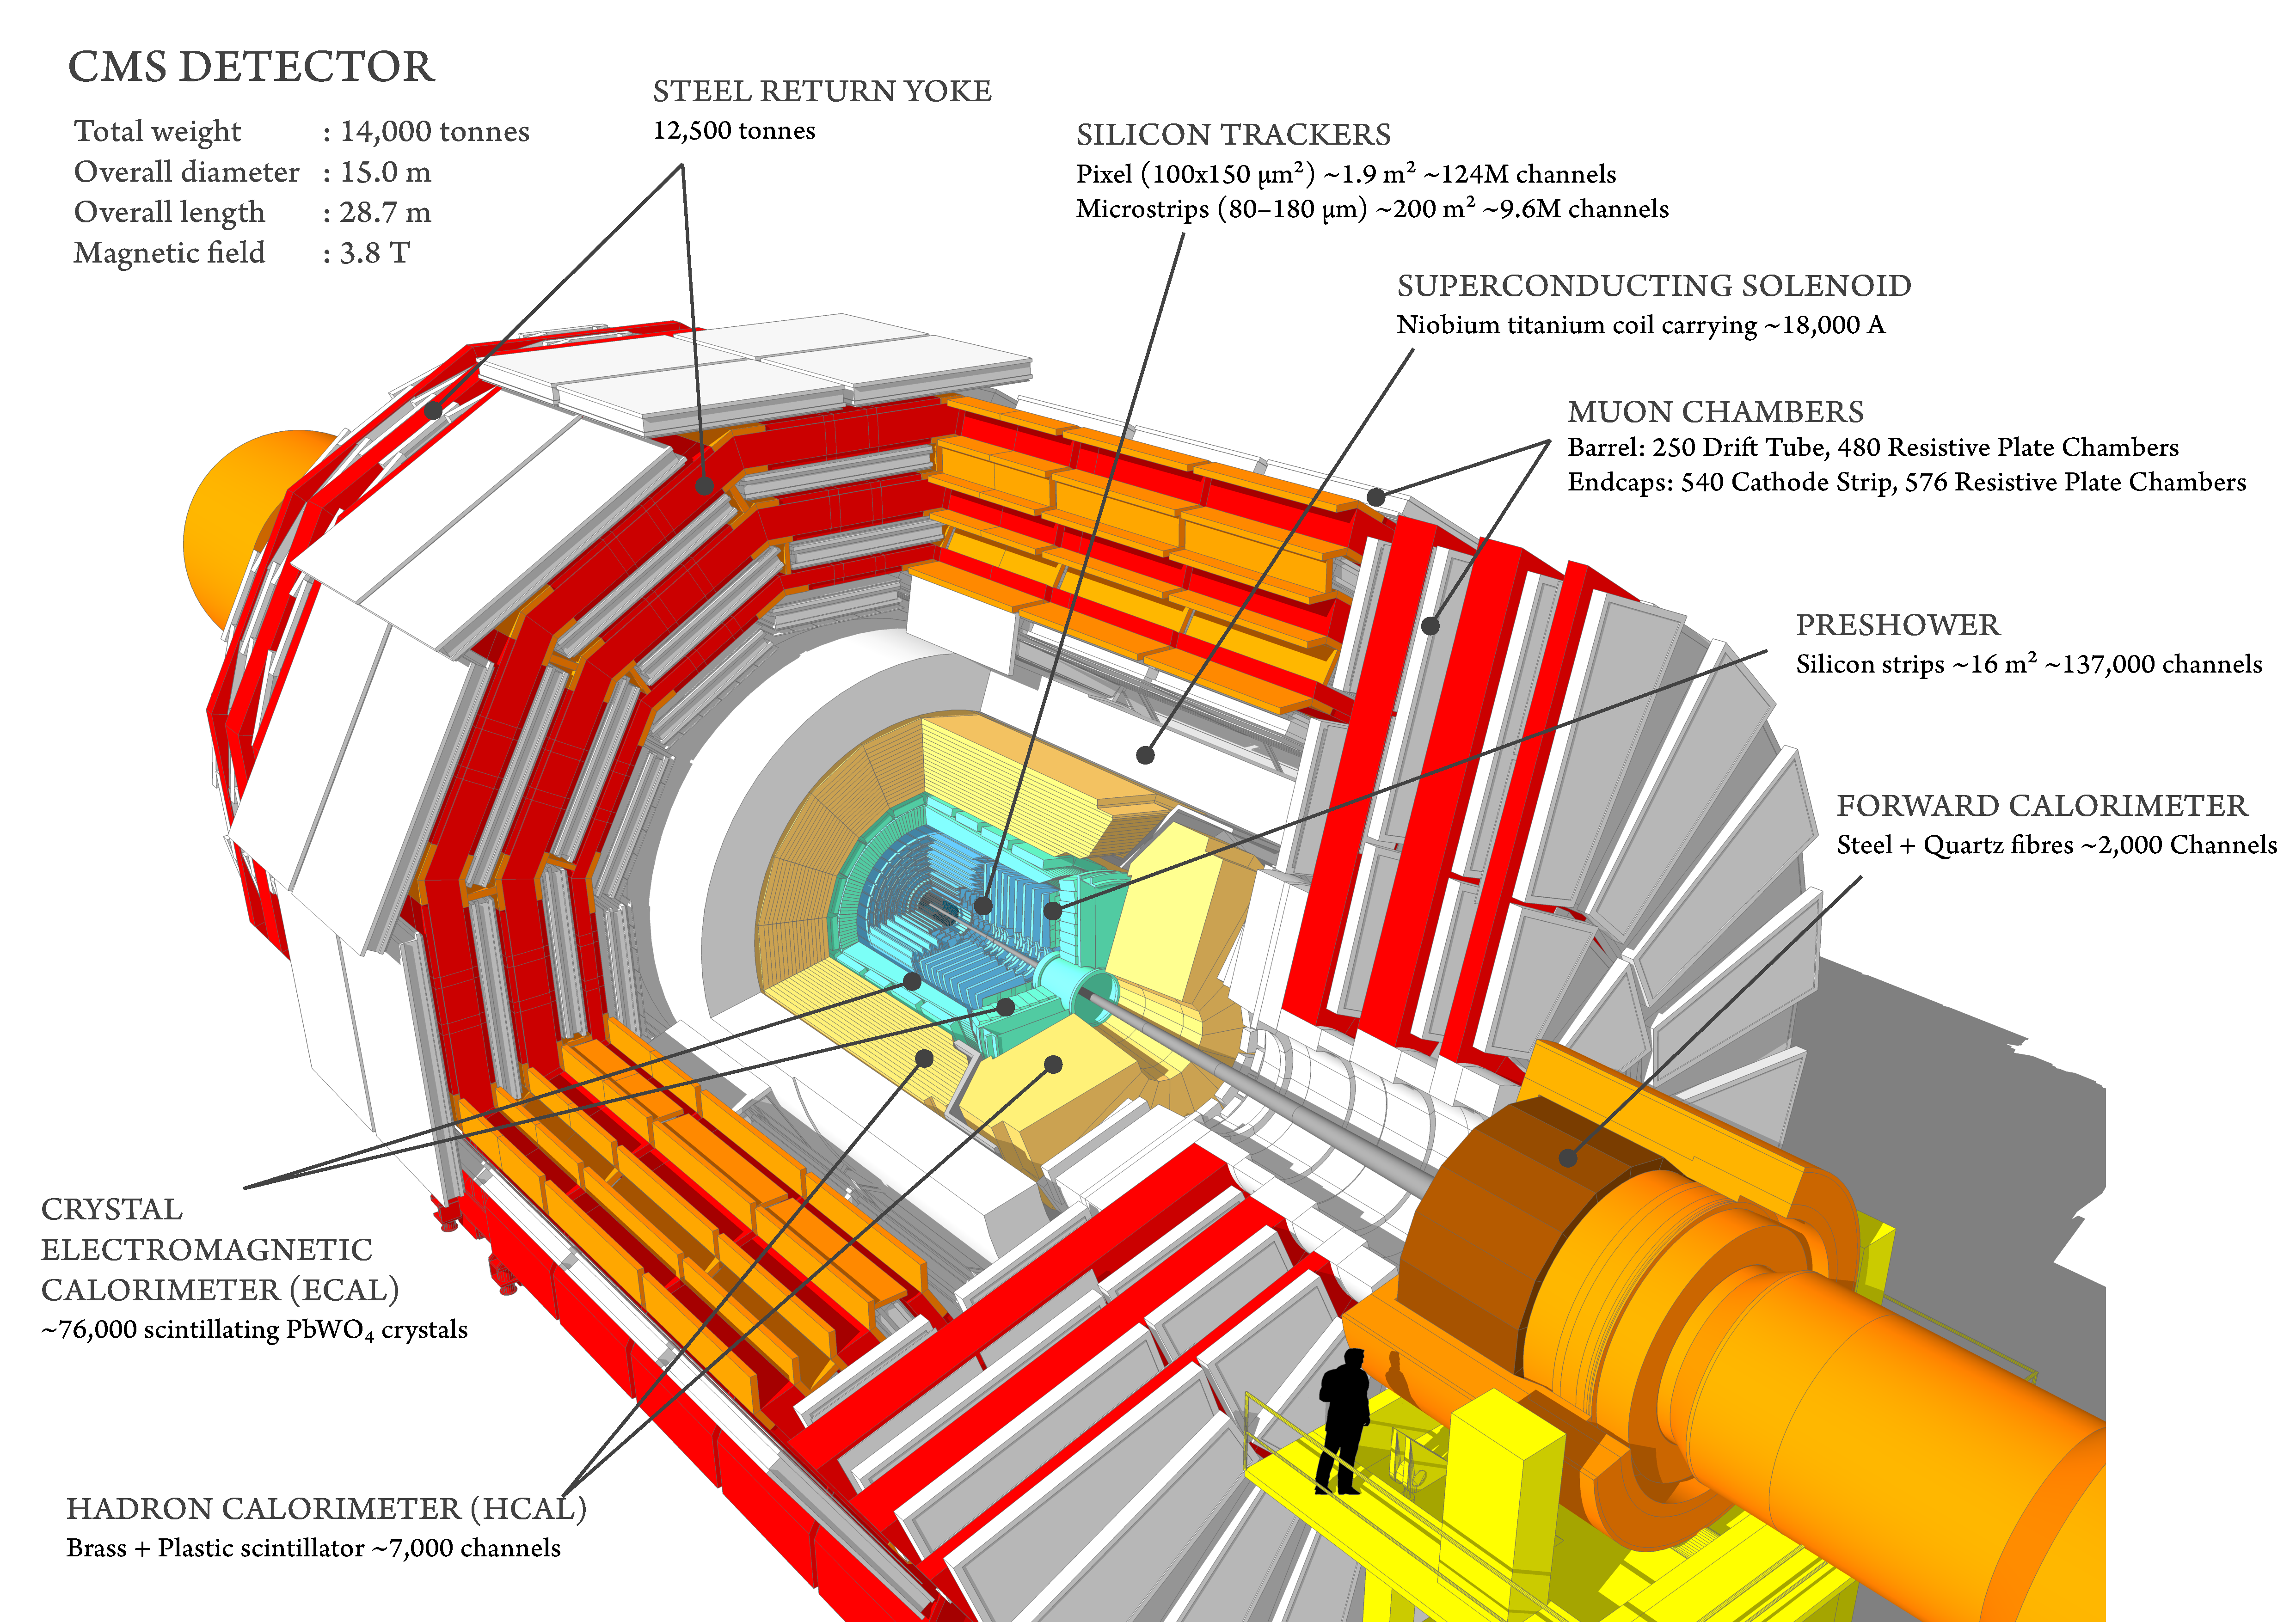
\includegraphics[width=0.85\textwidth]{fig/experiment/cms_cutaway.pdf}
  \caption{}
  \label{fig:CMSCut}
\end{figure}

\begin{figure}[htbp]
  \centering
  \includegraphics[width=0.85\textwidth]{fig/experiment/cms_crosssec.pdf}
  \caption{}
  \label{fig:CMSCrosssec}
\end{figure}

\subsection{Inner Tracking System}
\label{subsec:tracking}

\subsection{Calorimeters}
\label{subsec:calorimeter}

\subsection{Muon Tracking System}
\label{subsec:muonTrack}

\subsection{Trigger System and Data Acquisition}
\label{subsec:trigger}

% !TEX root = ../thesis.tex

\chapter{Search for a Heavy Diboson Resonance Produced via Vector Boson Fusion}
\label{chap:analysis}

\section{Introduction}

% Motivation of analysis from theory chapter
In chapter~\ref{chap:theory}, we explored some of the motivation behind BSM searches and examples of BSM theories that predict exotic new particles that may be found in collision events at accelerator facilities.
We also enumerated some of the benchmark models from BSM theories, which were the spin-0 Kaluza-Klein Radion, spin-1 $W'$/$Z'$ boson, and spin-2 Bulk Graviton.
Additionally, we discussed the VBF production mode that this work focuses on, and the final state that is produced.

% Previous searches
Previous searches have been conducted for dibosonic resonances at both CMS and ATLAS, although none have found evidence of such a resonance being observed at the LHC~\cite{Sirunyan_18,Aaboud_18,Aaboud_18_2,Aad_15,Khachatryan_14,Sirunyan_17,Sirunyan_17_2,atlas20}.
Some of these searches also considered different production modes, as well as other intermediate and final states, such as a $ZZ$/$ZH$ resonance with fully leptonic or hadronic final states.
As mentioned in section~\ref{sec:VBF}, this analysis is itself a continuation of a previous search by the CMS collaboration for a dibosonic resonance using data from 2016.

% VBF analysis as part of the main analysis
While this work focuses on the VBF production mode, it is one of three modes considered for the full diboson analysis using the Run 2 data.
The other two modes considered involve gluon-gluon fusion (\ggF) and Drell-Yan (\DY) processes.
These additional modes produce identical \lnuqqbarprp and \lnubbbar semileptonic final states, but without the VBF jets in the forward regions of the detector.
For completeness, we include the full diboson analysis with the non-VBF production categories in this chapter.
Figure~\ref{fig:nonVbf} shows some example Feynman diagrams of other processes that were considered for the full analysis.

\begin{figure}[htbp]
  \centering
  % !TEX root = ../../thesis.tex
\begin{tikzpicture}
  \begin{feynman}
    % Vertices
    \coordinate (g1) at (135:2.25);
    \coordinate (g2) at (225:2.25);
    \coordinate (x1) at (0,0);
    \coordinate (x2) at (1.5,0);
    \coordinate (v1) at ($(x2)+(45:1.5)$);
    \coordinate (v2) at ($(x2)+(-45:1.5)$);
    \coordinate (q1) at ($(v1)+(25:1.5)$);
    \coordinate (q2) at ($(v1)+(-25:1.5)$);
    \coordinate (l1) at ($(v2)+(25:1.5)$);
    \coordinate (l2) at ($(v2)+(-25:1.5)$);

    \coordinate (q3) at ($(g1)+(8,0)$);
    \coordinate (q4) at ($(g2)+(8,0)$);
    \coordinate (x3) at ($(x1)+(8,0)$);
    \coordinate (x4) at ($(x2)+(8,0)$);
    \coordinate (v3) at ($(v1)+(8,0)$);
    \coordinate (v4) at ($(v2)+(8,0)$);
    \coordinate (q5) at ($(q1)+(8,0)$);
    \coordinate (q6) at ($(q2)+(8,0)$);
    \coordinate (l3) at ($(l1)+(8,0)$);
    \coordinate (l4) at ($(l2)+(8,0)$);

    % Lines
    \draw[gluon] (x1) -- (g1);
    \draw[gluon] (x1) -- (g2);
    \draw[boson] ($(x1)+(0,-0.025)$) -- ($(x2)+(0,-0.025)$);
    \draw[boson] ($(x1)+(0,0.025)$) -- ($(x2)+(0,0.025)$) node[pos=0.5,above] {$X$};
    \draw[boson] (x2) -- (v1) node[pos=0.75,xshift=-0.5cm] {$W$};
    \draw[boson] (x2) -- (v2) node[pos=0.75,xshift=-0.5cm] {$W$};
    \draw[fermion] (v1) -- (q1);
    \draw[fermion] (q2) -- (v1);
    \draw[fermion] (v2) -- (l1);
    \draw[fermion] (l2) -- (v2);

    \draw[fermion] (q3) -- (x3);
    \draw[fermion] (x3) -- (q4);
    \draw[boson] (x3) -- (x4) node[pos=0.5,above] {$X$};
    \draw[scalar] (x4) -- (v3) node[pos=0.75,xshift=-0.5cm] {$H$};
    \draw[boson] (x4) -- (v4) node[pos=0.75,xshift=-0.5cm] {$W$};
    \draw[fermion] (v3) -- (q5);
    \draw[fermion] (q6) -- (v3);
    \draw[fermion] (v4) -- (l3);
    \draw[fermion] (l4) -- (v4);

    % Blobs
    \fill[white] (x1) circle (0.2);
    \fill[white] (x2) circle (0.2);
    \draw[pattern=north west lines] (x1) circle (0.2);
    \draw[pattern=north west lines] (x2) circle (0.2);

    \fill[white] (x3) circle (0.2);
    \fill[white] (x4) circle (0.2);
    \draw[pattern=north west lines] (x3) circle (0.2);
    \draw[pattern=north west lines] (x4) circle (0.2);

    % Label
    \node[anchor=mid,left] at (g1) {$g$};
    \node[anchor=mid,left] at (g2) {$g$};
    \node[anchor=mid,right] at (q1) {$q$};
    \node[anchor=mid,right] at (q2) {$\bar{q}'$};
    \node[anchor=mid,right] at (l1) {$\ell$};
    \node[anchor=mid,right] at (l2) {$\bar{\nu}$};

    \node[anchor=mid,left] at (q3) {$q$};
    \node[anchor=mid,left] at (q4) {$\bar{q}'$};
    \node[anchor=mid,right] at (q5) {$b$};
    \node[anchor=mid,right] at (q6) {$\bar{b}$};
    \node[anchor=mid,right] at (l3) {$\ell$};
    \node[anchor=mid,right] at (l4) {$\bar{\nu}$};
  \end{feynman}
\end{tikzpicture}

  \caption{
    Examples of additional production processes considered in the full analysis that includes non-VBF production modes.
    We also consider a gluon-gluon fusion process such as a neutral spin-2 resonance decaying to $WW$ (left), and a Drell-yan process such as a charged spin-1 resonance decaying to $WH$ (right).
  }
  \label{fig:nonVbf}
\end{figure}

% Details of reconstructing events
In subsection~\ref{subsec:expEvent} we discussed the expected event structure for the decay events of interest, in which the leptonic decay of the $W$ boson results in an $e\nu$ or $\mu\nu$ pair with large missing transverse energy from the neutrino, the hadronic decay of the $V$/$H$ boson results in a large single jet with substructure, and VBF processes produce forward-facing jets.
The boosted topology is a result of the fact that the resonances considered have masses in the TeV range, which causes the $W$ and $V$/$H$ bosons to have transverse momenta on the order of several hundred GeV.
This requires the use of specialized techniques to identify and reconstruct the individual $W$ and $V$/$H$ bosons based on information from the reconstructed lepton, missing transverse energy of the neutrino, and two-pronged substructure of the jet.
Additionally, the signal models used for the analysis assume that the resonance width is narrow, meaning that the decay width of the resonance in the $WV$/$WH$ diboson mass spectrum is smaller than the experimental resolution.

% Details on modeling background
A unique aspect of the previous analysis that this work inherits is a novel signal extraction method, in which the SM background contribution is estimated from the data using a two-dimensional (2D) maximum likelihood fit.
This process is performed in the plane formed by the mass of the jet from the $V$/$H$ decay \MJ, and the invariant mass of the $WV$/$WH$ diboson system \MVV.
Two classes of SM background events are considered for this analysis.
The first is a \WVt background that is resonant in the \MJ spectrum, and the second is a \Wjets contribution that is non-resonant in \MJ.
One advantage of using a 2D fit is the ability to retain more events for modeling background in the sideband regions within the 2D \MJ-\MVV plane, as opposed to looking at the sidebands in the \MJ and \MVV spectra separately.
This also allows for conducting a simultaneous search of $WW$, $WZ$, and $WH$ resonances as opposed to performing separate analyses in pre-defined \MJ windows.

% Chapter overview
For this chapter, we examine the complete analysis process of the search for a dibosonic resonance produced in proton-proton collisions at the LHC with center-of-mass energies of $\sqrt{s}=13\unit{TeV}$.
The data used in this analysis were collected over 2016, 2017, and 2018 with integrated luminosities of $35.9\unit{fb^{-1}}$, $41.5\unit{fb^{-1}}$, and $59.7\unit{fb^{-1}}$, respectively.
Section~\ref{sec:samples} provides an overview of the data and simulation samples that were used for the analysis.
In section~\ref{sec:events}, we discuss the selection cuts used to determine which events are used from the data and simulation samples.
We then go over the SM sources of background and how they are taken into account for the analysis in section~\ref{sec:bkg}, followed by the signal modeling process in section~\ref{sec:sig}.
The fit validation and bias testing procedures are described in section~\ref{sec:bias}, after which we discuss the results of the search in section~\ref{sec:results}.

\section{Data and Simulation Samples}
\label{sec:samples}

% The need for simulation samples of signal and background
This search uses the proton-proton collision data collected by the CMS detector during Run 2.
The data are collected and stored for analysis after events generate trigger primitives in the detector subsystems and get passed through the HLT as described in chapter~\ref{chap:exp}.
We also list the signal samples used in the analysis that are based on the BSM models of subsection~\ref{subsec:benchmark}.
Additionally, we list the samples that model SM background contributions to the search.
Complete lists of each sample used are found in appendix~\ref{chap:appendixSamples}.

% Data samples
The data are listed in tables~\ref{tab:dataSamples2016}-\ref{tab:dataSamples2018}, along with their integrated luminosities.
For each year of Run 2, documentation is available for the luminosity measurements~\cite{CMS-PAS-LUM-17-001,CMS-PAS-LUM-17-004,CMS-PAS-LUM-18-002}.
The data are divided into three sets per year, with contributions from the \texttt{SingleMuon}, \texttt{SingleElectron}, and \texttt{MET} sets.

% Signal samples
This analysis makes use of ten benchmark signal models, which are listed in tables~\ref{tab:ggFGBulkToWWSamples}-\ref{tab:VBFZprToWWSamples} with their cross sections and branching ratios.
The signal models used are \ggF/\VBF\GBulktoWWtolnuqqbarpr, \ggF/\VBF\RadtoWWtolnuqqbarpr, \DY/\VBF\WprtoWZtolnuqqbar, \DY/\VBF\WprtoWHtolnubbbar, and \DY/\VBF\ZprtoWWtolnuqqbarpr.
Each signal has different samples for each year of Run 2, for a total of three sets of samples per signal.
Furthermore, each signal has separate samples with 50,000 events for the following resonance masses: 0.8, 1, 1.2, 1.4, 1.6, 1.8, 2.0, 2.5, 3.0, 3.5, 4.0, and $4.5\unit{TeV}$\footnote{The 2016 \VBF\ZprtoWW and 2016 \VBF\WprtoWZ sets are the exception to this, lacking mass values below $1.2\unit{TeV}$.}.
Additional details on the parameters for each model are discussed in section~\ref{sec:sigSamples} of appendix~\ref{chap:appendixSamples}.

% Background samples
Finally, samples are also used to simulate SM background contributions, as listed in tables~\ref{tab:bkg2016Samples} and \ref{tab:bkg2017Samples} along with their cross sections.
These background samples include various processes that are broadly categorized as \Wjets and \WVt, some of which include DY+jets, QCD, and $t\bar{t}$ production samples.
% More on background samples

\section{Event Selection}
\label{sec:events}

% Goal of event selection
In subsection~\ref{subsec:expEvent}, we described the expected event topology for the $WV$/$WH$ dibosonic resonance that this work searches for.
In particular, the semileptonic decay produces a highly energetic lepton ($e$ or $\mu$) and large \Etmiss from the neutrino from the \Wtolnu decay, a large-radius jet from the hadronic \Vtoqqbarpr or \Htobbbar decay, and forward-facing VBF jets for VBF-produced resonances.
To select for possible events that exhibit the expected final state structure, selection cuts must be made that capture the expected behavior and reduce background.
This section provides an overview of the cuts that were made in the analysis to optimize the search for the $WV$/$WH$ dibosonic resonance.

\subsection{Trigger}

% Trigger paths
There are multiple HLT trigger paths that used for recording the data that this analysis uses.
Most of the data are collected from the single electron and single muon triggers, with the remainder coming from the single photon, EGamma, and MET triggers.
For each year we use different paths, which are listed in tables~\ref{tab:triggers2016}, \ref{tab:triggers2017}, and \ref{tab:triggers2018} for the years 2016, 2017, and 2018, respectively.

\begin{table}[htbp]
  \centering
  % !TEX root = ../../thesis.tex
\scriptsize
\begin{tabular}{l|l|c}
  \hline
  Dataset        & HLT paths                                    & Description\\
  \hline \hline
  \ttfamily SingleElectron/& \ttfamily HLT\_Ele27\_WPTight\_Gsf\_v*                 & $\pt>27\unit{GeV}$, Tight WP for ele ID  \\
  \ttfamily SinglePhoton   & \ttfamily OR HLT\_Ele45\_WPLoose\_Gsf\_v*              & $\pt>45\unit{GeV}$, Loose WP for ele ID  \\
                 & \ttfamily OR HLT\_Ele115\_CaloIdVT\_GsfTrkIdT\_v*      & $\pt>115\unit{GeV}$  \\
                 & \ttfamily OR HLT\_Photon175\_v*                        & $\Et>175\unit{GeV}$  \\
  \hline
  \ttfamily SingleMuon     & \ttfamily HLT\_Mu50\_v*                                & $\pt>50\unit{GeV}$ \\
                 & \ttfamily OR HLT\_TkMu50\_v*                           & tracker muon, $\pt>50\unit{GeV}$ \\
  \hline
  \ttfamily MET            & \ttfamily HLT\_PFMETNoMu120\_PFMHTNoMu120\_IDTight\_v* & $\Etmiss>120\unit{GeV}$ \\
  \hline
\end{tabular}

  \caption{
    HLT paths used in 2016 data and MC.
  }
  \label{tab:triggers2016}
\end{table}

\begin{table}[htbp]
  \centering
  % !TEX root = ../../thesis.tex
\scriptsize
\begin{tabular}{l|l|c}
  \hline
  Dataset        & HLT paths                                    & Description\\
  \hline \hline
  \ttfamily SingleElectron/& \ttfamily HLT\_Ele32\_WPTight\_Gsf\_v*                 & $\pt>32\unit{GeV}$, Tight WP for ele ID  \\
  \ttfamily SinglePhoton   & \ttfamily OR HLT\_Ele35\_WPTight\_Gsf\_v*              & $\pt>35\unit{GeV}$, Tight WP for ele ID  \\
                 & \ttfamily OR HLT\_Ele115\_CaloIdVT\_GsfTrkIdT\_v*      & $\pt>115\unit{GeV}$  \\
                 & \ttfamily OR HLT\_Photon200\_v*                        & $\Et>200\unit{GeV}$  \\
  \hline
  \ttfamily SingleMuon     & \ttfamily HLT\_Mu50\_v*                                & $\pt>50\unit{GeV}$ \\
                 & \ttfamily OR HLT\_OldMu100\_v*                         & $\pt>100\unit{GeV}$ \\
                 & \ttfamily OR HLT\_TkMu100\_v*                          & tracker muon, $\pt>100\unit{GeV}$ \\
  \hline
  \ttfamily MET            & \ttfamily HLT\_PFMETNoMu120\_PFMHTNoMu120\_IDTight\_v* & $\Etmiss>120\unit{GeV}$ \\
  \hline
\end{tabular}

  \caption{
    HLT paths used in 2017 data and MC.
  }
  \label{tab:triggers2017}
\end{table}

\begin{table}[htbp]
  \centering
  \input{tab/analysis/triggers2018.tex}
  \caption{
    HLT paths used in 2018 data and MC.
  }
  \label{tab:triggers2018}
\end{table}

% Single electron thresholds
The single electron \pt thresholds used are 27, 45, and $115\unit{GeV}$ for 2016, 32, 25, and $115\unit{GeV}$ for 2017, and 25 and $115\unit{GeV}$ for 2018. % Check why the threshold is 25 and not 32 for 2018
Additionally, we apply an OR with \texttt{HLT\_Photon175} in 2016 with an \Et threshold of $175\unit{GeV}$, as well as with \texttt{HLT\_Photon200} in 2017 with $200\unit{GeV}$. % Need to find out what an OR is
These thresholds were applied as recommended by the CMS E/Gamma Physics Object Group (POG)~\cite{MuonPOG}.

% Single muon thresholds
For the muon thresholds, the main threshold is $50\unit{GeV}$ across all three years, with an OR for \texttt{HLT\_TkMu50} at $50\unit{GeV}$ in 2016, and an OR for \texttt{HLT\_OldMu100} in 2017 and \texttt{HLT\_TkMU100} in 2018 at $100\unit{GeV}$, as recommended by the Muon POG~\cite{MuonHLT2016,MuonHLT2017,MuonHLT2018}.

% Additional explanation of efficiencies?
% Possibly add subsection on prefiring weights

\subsection{Pileup Reweighting}

The data samples from all three Run 2 years have different pileup (PU) profiles than that of the simulation samples that were used for this analysis.
In order to account for this, we compute and apply PU weights to our samples and compare distributions for the number of primary vertices both with and without weights to the data.
Figure~\ref{fig:PUreweight} shows these distributions for 2016, 2017, and 2018.
The weights are computed using the recommended minimum bias cross section of $69.2\unit{mb}$. % Citation needed

\begin{figure}[htbp]
  \centering
  \includegraphics[width=0.45\textwidth]{fig/analysis/PUrewN_0_2016_nVert.pdf}
  \includegraphics[width=0.45\textwidth]{fig/analysis/PUrewN_0_2017_nVert.pdf}\\
  \includegraphics[width=0.45\textwidth]{fig/analysis/PUrewN_0_2018_nVert.pdf}
  \caption{
    Distribution of the number of primary vertices reconstructed in simulation before and after pileup reweighting, with data present, for 2016 (top left), 2017 (top right), and 2018 (bottom).
  }
  \label{fig:PUreweight}
\end{figure}

\subsection{Muon Selection}

% High-pT muon selection criteria
When selecting muons for the analysis, they must pass the following high-\pt muon identification criteria as provided by the CMS Muon POG~\cite{MuonSelection}:
\begin{itemize}
  \item The muon is reconstructed as a ``global'' muon.
  \item At least one muon-chamber hit included in the global-muon track fit or in the TuneP fit.
  \item Muon segments in at least two muon stations.
  \item The \pt relative error ($\sigma(\pt)/\pt$) of the muon best track is less than 30\%.
  \item Its tracker track has transverse impact parameter $d_{xy}<2\unit{mm}$ with respect to the primary vertex.
  \item The longitudinal distance of the tracker with respect to the primary vertex is $d_z<5\unit{mm}$.
  \item The muon track has at least one pixel hit.
  \item The muon track has at least six tracker layer hits.
\end{itemize}

% Further muon selection
In addition to the high-\pt muon identification criteria, for this analysis we also require each muon to have $\pt>55\unit{GeV}$ and to be confined to the region $|\eta|<2.4$.
We also apply an isolation requirement on the muons in order to further suppress background.
This is done using the full relative particle flow isolation using $\Delta\beta$ corrections, with the requirement that $I_\mathrm{rel}<0.05$.

Scale factors for muon ID as provided by the Muon POG are also applied~\cite{MuonPAGs}.
To appropriately apply these scale factors as they vary by year to the full Run 2 data set, we weight them by the fraction of integrated luminosity for each year.
We also apply a scale factor for the isolation requirement, which is shown in figure~\ref{fig:muonIsoSF}.
This scale factor was derived on top of muon high-\pt ID, in boosted $Z$ and DY events over the full Run 2 period, which is found to be within 1\% from unity and smaller than the systematic uncertainty for the muon trigger/reco/ID of 5\% used in signal extraction.

\begin{figure}[htbp]
  \centering
  \includegraphics[width=0.65\textwidth]{fig/analysis/muonFullIsoSF.pdf}
  \caption{
    Efficiency in data and simulation and data/MC scale factor for muon isolation requirement.
  }
  \label{fig:muonIsoSF}
\end{figure}

\subsection{Electron Selection}

% Electron reconstruction
The electrons that are reconstructed from trigger primitives in the ECAL are required to pass the ``HEEP v7.0'' ID requirements as prescribed by the E/Gamma POG~\cite{HEEPV70}.
The ID requirements ensure that the reconstructed electrons from the ECAL energy deposits are paired with a high quality track from the inner tracker and have a shape consistent with an electromagnetic shower in the calorimeter.
These requirements are listed in table~\ref{tab:HEEPV70}.
For our analysis, we also require them to have $\pt>55\unit{GeV}$ and be within the pseudorapidity range $|\eta|<2.5$, except for the region $[1.4442,1.566]$. % Unsure why this range is excluded
We also apply scale factors for the HEEP ID requirements along with RECO scale factors as recommended by the E/Gamma POG~\cite{EgammaScale}.

\begin{table}[htbp]
  \centering
  % !TEX root = ../../thesis.tex
\footnotesize
\begin{tabular}{l|l|l}
  \hline
  Variable & Barrel & Endcap \\
  \hline
  \hline
  \multicolumn{3}{c}{Acceptance selections} \\
  \hline
  \Et & $\Et>35\unit{GeV}$ & $\Et>35\unit{GeV}$ \\
  $\eta$ & $|\eta_\mathrm{SC}|<1.4442$ & $1.566<|\eta_\mathrm{SC}|<2.5$ \\
  \hline
  \multicolumn{3}{c}{Identification selections}  \\
  \hline
  \texttt{isEcalDriven} & \texttt{true} & \texttt{true} \\
  $\Delta\eta_\mathrm{in}^\mathrm{seed}$ & $|\Delta\eta_\mathrm{in}^\mathrm{seed}|<0.004$ & $|\Delta\eta_\mathrm{in}^\mathrm{seed}|<0.006$ \\
  $\Delta\phi_\mathrm{in}$ & $|\Delta\phi_\mathrm{in}|<0.06$ & $|\Delta\phi_\mathrm{in}|<0.06$ \\
  $H/E$ & $H/E<1/E+0.05$ & $H/E<5/E+0.05$ \\
  $\sigma_{i\eta i\eta}$ & - & $\sigma_{i\eta i\eta}<0.03$ \\
  $\frac{E_{1\times5}}{E_{5\times5}}$, $\frac{E_{2\times5}}{E_{5\times5}}$ & $\frac{E_{1\times5}}{E_{5\times5}}>0.83$ or $\frac{E_{2\times5}}{E_{5\times5}}>0.94$ & - \\
  Inner lost layer hits & lost hits $\leq1$ & lost hits $\leq1$ \\
  Impact parameter, $d_{xy}$ & $|d_{xy}|<0.02$ & $|d_{xy}|<0.05$ \\
  \hline
  \multicolumn{3}{c}{Isolation selections}\\
  \hline
  EM + had depth 1 & $I<2+0.03\Et+0.28\rho$ & $I<2.5+0.28\rho$ ($\Et<50\unit{GeV}$) \\
  isolation, $I$ & & else $I<2.5+0.03(\Et-50\unit{GeV})+0.28\rho$ \\
  $\pt$ isolation, $I_{\pt}$ & $I_{\pt}<5\unit{GeV}$ & $I_{\pt}<5\unit{GeV}$ \\
  \hline
\end{tabular}

  \caption{
    Definitions of HEEP ID V7.0 selections.
  }
  \label{tab:HEEPV70}
\end{table}

\subsection{Jet Selection}

%\begin{figure}[htbp]
%  \centering
%  % !TEX root = ../../thesis.tex

\begin{tikzpicture}
  % Main jet
  \draw[rotate around={270:(0,0)},dotted,thick] (0,7) ellipse (2.6 and 1.3);
  \draw[rotate around={270:(0,0)},dotted,thick] (0,0) -- (69.29:7.21);
  \draw[rotate around={270:(0,0)},dotted,thick] (0,0) -- (110.71:7.21);

  % Subjets
  \draw[rotate around={270:(0,0)},dotted,thick] (1.25,7) ellipse (0.975 and 0.4875);
  \draw[rotate around={270:(0,0)},dotted,thick] (0,0) -- (72.275:7.26);
  \draw[rotate around={270:(0,0)},dotted,thick] (0,0) -- (87.75:7.01);
  \draw[rotate around={270:(0,0)},dotted,thick] (-1.25,7) ellipse (0.975 and 0.4875);
  \draw[rotate around={270:(0,0)},dotted,thick] (0,0) -- (92.25:7.01);
  \draw[rotate around={270:(0,0)},dotted,thick] (0,0) -- (107.725:7.26);

  % Axes
  \draw[->,thick] (0,0) -- (10.12:8.5) node[right] {$\hat{n}_1$};
  \draw[->,thick] (0,0) -- (-10.12:8.5) node[right] {$\hat{n}_2$};
\end{tikzpicture}

%  \caption{
%    Illustration of jet substructure for a two-pronged jet with axes $\mathbf{\hat{n}}_1$ and $\mathbf{\hat{n}}_2$.
%  }
%  \label{fig:jet}
%\end{figure}

\subsection{Missing Transverse Energy}

\subsection{VBF Forward Jets}

\subsection{Spin Polarization and Boson Rapidities}

\subsection{Event Categorization}

\section{Background Modeling}
\label{sec:bkg}

%\begin{figure}[htbp]
%  \centering
%  % !TEX root = ../../thesis.tex

\begin{tikzpicture}
  \begin{feynman}
    % Vertices
    \coordinate (q1) at (135:2.25);
    \coordinate (q2) at (0,0);
    \coordinate (q3) at (225:2.25);
    \coordinate (l1) at ($(q3)+(5,0)$);
    \coordinate (l2) at ($(l1)+(-25:-1.5)$);
    \coordinate (l3) at ($(l2)+(25:1.5)$);
    \coordinate (g1) at (135:0.5625);
    \coordinate (q4) at ($(q1)+(5,0)$);
    \coordinate (q5) at ($(q4)+(25:-1.5)$);
    \coordinate (q6) at ($(q5)+(-25:1.5)$);

    \coordinate (g2) at ($(7,0)+(135:1.5)$);
    \coordinate (g3) at (7,0);
    \coordinate (g4) at ($(7,0)+(225:1.5)$);
    \coordinate (q7) at (8.5,0);
    \coordinate (q8) at ($(q7)+(55:1.5)$);
    \coordinate (q9) at ($(q7)+(-55:1.5)$);
    \coordinate (q10) at ($(q8)+(-15:1.5)$);
    \coordinate (l4) at ($(q9)+(15:1.5)$);
    \coordinate (q11) at ($(q8)+(15:1.5)$);
    \coordinate (q12) at ($(q9)+(-15:1.5)$);
    \coordinate (q13) at ($(q10)+(15:1.5)$);
    \coordinate (q14) at ($(q10)+(-15:1.5)$);
    \coordinate (l5) at ($(l4)+(15:1.5)$);
    \coordinate (l6) at ($(l4)+(-15:1.5)$);

    % Lines
    \draw[fermion] (q1) -- (q2);
    \draw[fermion] (q2) -- (q3);
    \draw[gluon] (g1) -- (q5) node[pos=0.5,above] {$g$};
    \draw[boson] (q2) -- (l2) node[pos=0.5,below] {$W$};
    \draw[fermion] (q5) -- (q4);
    \draw[fermion] (q6) -- (q5);
    \draw[fermion] (l2) -- (l1);
    \draw[fermion] (l3) -- (l2);

    \draw[gluon] (g2) -- (g3);
    \draw[gluon] (g3) -- (g4);
    \draw[gluon] (g3) -- (q7) node[pos=0.5,below] {$g$};
    \draw[fermion] (q7) -- (q8) node[pos=0.5,left] {$q$};
    \draw[fermion] (q9) -- (q7) node[pos=0.5,left] {$\bar{q}$};
    \draw[boson] (q8) -- (q10) node[pos=0.5,below] {$W$};
    \draw[boson] (q9) -- (l4) node[pos=0.5,above] {$W$};
    \draw[fermion] (q8) -- (q11);
    \draw[fermion] (q12) -- (q9);
    \draw[fermion] (q10) -- (q13);
    \draw[fermion] (q14) -- (q10);
    \draw[fermion] (l4) -- (l5);
    \draw[fermion] (l6) -- (l4);

    % Labels
    \node[anchor=mid,left] at (q1) {$q$};
    \node[anchor=mid,left] at (q3) {$\bar{q}'$};
    \node[anchor=mid,right] at (q4) {$q$};
    \node[anchor=mid,right] at (q6) {$\bar{q}$};
    \node[anchor=mid,right] at (l1) {$\ell$};
    \node[anchor=mid,right] at (l3) {$\bar{\nu}$};
    \node at (0.909,2.75) {$W$+jets};

    \node[anchor=mid,left] at (g2) {$g$};
    \node[anchor=mid,left] at (g4) {$g$};
    \node[anchor=mid,right] at (q11) {$b$};
    \node[anchor=mid,right] at (q12) {$\bar{b}$};
    \node[anchor=mid,right] at (q13) {$q''$};
    \node[anchor=mid,right] at (q14) {$\bar{q}'$};
    \node[anchor=mid,right] at (l5) {$\ell$};
    \node[anchor=mid,right] at (l6) {$\bar{\nu}$};
    \node at (9.099,2.75) {$W$+$V$/$t$};
  \end{feynman}
\end{tikzpicture}

%  \caption{
%    Feynman diagrams of the two main SM sources of background to consider for the search.
%    Both cases produce a final state that is similar to the expected final state produced by the VBF signal process.
%    The most common background is the \Wjets process (left), followed by the \WVt process (right).
%  }
%  \label{fig:bkgFeynman}
%\end{figure}

\section{Signal Modeling}
\label{sec:sig}

\section{Fit Validation and Bias Testing}
\label{sec:bias}

\section{Results}
\label{sec:results}

% !TEX root = ../thesis.tex

\section{Data and Simulation Samples}
\label{sec:samples}

% The need for simulation samples of signal and background
This search uses the proton-proton collision data collected by the CMS detector during Run 2.
The data are collected and stored for analysis after events generate trigger primitives in the detector subsystems and get passed through the HLT as described in chapter~\ref{chap:exp}.
We also list the MC signal samples used in the analysis that are based on the BSM models of subsection~\ref{subsec:benchmark}.
Additionally, we list the MC samples that model SM background contributions to the search.

\subsection{Data Samples}

% Data samples
The data used for this work are based on three different sets over the three Run 2 years of 2016, 2017, and 2018.
For each year of Run 2, documentation is available for the luminosity measurements~\cite{CMS-PAS-LUM-17-001,CMS-PAS-LUM-17-004,CMS-PAS-LUM-18-002}.
The full dataset is divided into three sets per year, with contributions from the \texttt{SingleMuon}, \texttt{SingleElectron}, and \texttt{MET} sets.
The 2016 Rereco (Re-MiniAOD 03Feb2017) set for Run2016B-H with an integrated luminosity of $35.9\unit{fb^{-1}}$ is listed in table~\ref{tab:dataSamples2016}.
For 2017, the Rereco (31Mar2018) set for Run2017B-F with $41.5\unit{fb^{-1}}$ is listed in table~\ref{tab:dataSamples2017}.
Finally, the 2018 Rereco (17Sep2018 for Run2018A-C, 22Jan2019 for Run2018D) with $59.7\unit{fb^{-1}}$ is listed in table~\ref{tab:dataSamples2018}\footnote{This set excludes the PromptReco for MET 2018D.}.
The golden data JSON certificates used are the following:
\begin{itemize}
  \item[2016:]
  \begingroup
  \fontsize{9pt}{12pt}
  \begin{verbatim}
  /afs/cern.ch/cms/CAF/CMSCOMM/COMM_DQM/certification/Collisions16/13TeV/ReReco/Final
   /Cert_271036-284044_13TeV_23Sep2016ReReco_Collisions16_JSON.txt
  \end{verbatim}
  \endgroup
  \item[2017:]
  \begingroup
  \fontsize{9pt}{12pt}
  \begin{verbatim}
  /afs/cern.ch/cms/CAF/CMSCOMM/COMM_DQM/certification/Collisions17/13TeV/ReReco
   /Cert_294927-306462_13TeV_EOY2017ReReco_Collisions17_JSON_v1.txt
  \end{verbatim}
  \endgroup
  \item[2018:]
  \begingroup
  \fontsize{9pt}{12pt}
  \begin{verbatim}
  /afs/cern.ch/cms/CAF/CMSCOMM/COMM_DQM/certification/Collisions18/13TeV/ReReco
   /Cert_314472-325175_13TeV_17SeptEarlyReReco2018ABC_PromptEraD_Collisions18_JSON.txt
  \end{verbatim}
  \endgroup
\end{itemize}

\begin{table}[htbp]
  \centering
  % !TEX root = ../../thesis.tex
\footnotesize
\begin{tabular}{lrr}
  \hline
  \textbf{Sample name} \\
  \hline
  \ttfamily/SingleMuon-{}-SingleElectron-{}-MET/Run2016B-03Feb2017-v3/MINIAOD \\
  \ttfamily/SingleMuon-{}-SingleElectron-{}-MET/Run2016C-03Feb2017-v1/MINIAOD \\
  \ttfamily/SingleMuon-{}-SingleElectron-{}-MET/Run2016D-03Feb2017-v1/MINIAOD \\
  \ttfamily/SingleMuon-{}-SingleElectron-{}-MET/Run2016E-03Feb2017-v1/MINIAOD \\
  \ttfamily/SingleMuon-{}-SingleElectron-{}-MET/Run2016F-03Feb2017-v1/MINIAOD \\
  \ttfamily/SingleMuon-{}-SingleElectron-{}-MET/Run2016G-03Feb2017-v1/MINIAOD \\
  \ttfamily/SingleMuon-{}-SingleElectron-{}-MET/Run2016H-03Feb2017-v2/MINIAOD \\
  \ttfamily/SingleMuon-{}-SingleElectron-{}-MET/Run2016H-03Feb2017-v3/MINIAOD \\
  \hline
\end{tabular}

  \caption{
    2016 data samples for Run2016B-H with $35.9\unit{fb^{-1}}$.
  }
  \label{tab:dataSamples2016}
\end{table}
\begin{table}[htbp]
  \centering
  % !TEX root = ../../thesis.tex
\footnotesize
\begin{tabular}{lrr}
  \hline
  \textbf{Sample name} \\
  \hline
  \ttfamily/SingleMuon-{}-SingleElectron-{}-MET/Run2017B-31Mar2018-v1/MINIAOD \\
  \ttfamily/SingleMuon-{}-SingleElectron-{}-MET/Run2017C-31Mar2018-v1/MINIAOD \\
  \ttfamily/SingleMuon-{}-SingleElectron-{}-MET/Run2017D-31Mar2018-v1/MINIAOD \\
  \ttfamily/SingleMuon-{}-SingleElectron-{}-MET/Run2017E-31Mar2018-v1/MINIAOD \\
  \ttfamily/SingleMuon-{}-SingleElectron-{}-MET/Run2017F-31Mar2018-v1/MINIAOD \\
  \hline
\end{tabular}

  \caption{
    2017 data samples for Run2017B-F with $41.5\unit{fb^{-1}}$.
  }
  \label{tab:dataSamples2017}
\end{table}

\begin{table}[htbp]
  \centering
  % !TEX root = ../../thesis.tex
\scriptsize
\begin{tabular}{lrr}
  \hline
  \textbf{Sample name} \\
  \hline
  \ttfamily /SingleMuon-{}-EGamma-{}-MET/Run2018A-17Sep2018-v2/MINIAOD \\
  \ttfamily /SingleMuon-{}-EGamma-{}-MET/Run2018B-17Sep2018-v1/MINIAOD \\
  \ttfamily /SingleMuon-{}-EGamma-{}-MET/Run2018C-17Sep2018-v1/MINIAOD \\
  \ttfamily /SingleMuon-{}-EGamma/Run2018D-22Jan2019-v2/MINIAOD \\
  \ttfamily /MET/Run2018D-PromptReco-v*/MINIAOD \\
  \hline
\end{tabular}

  \caption{
    2018 data samples for Run2018A-C and Run2018D with $59.7\unit{fb^{-1}}$.
  }
  \label{tab:dataSamples2018}
\end{table}

\subsection{Signal Samples}
\label{sec:sigSamples}

% Signal samples
This analysis makes use of ten benchmark signal models, which are listed in tables~\ref{tab:ggFGBulkToWWSamples}-\ref{tab:VBFZprToWWSamples} with their cross sections and branching ratios where appropriate.
The signal models used are \ggF/\VBF\GBulktoWWtolnuqqbarpr, \ggF/\VBF\RadtoWWtolnuqqbarpr, \DY/\VBF\WprtoWZtolnuqqbar, \DY/\VBF\WprtoWHtolnubbbar, and \DY/\VBF\ZprtoWWtolnuqqbarpr.
Each signal has different samples with 50,000 events for each year of Run 2, for a total of three sets of samples per signal.
Furthermore, each signal has separate samples with 50,000 events for the following resonance masses: 0.8, 1, 1.2, 1.4, 1.6, 1.8, 2.0, 2.5, 3.0, 3.5, 4.0, and $4.5\unit{TeV}$\footnote{The 2016 \VBF\ZprtoWW and 2016 \VBF\WprtoWZ sets are the exception to this, lacking mass values below $1.2\unit{TeV}$.}.
The 2016 \VBF\ZprtoWW and 2016 \VBF\WprtoWZ samples do not have mass values below $1.2\unit{TeV}$, and some samples have masses that extend from $4.5\unit{TeV}$ to $8\unit{TeV}$ in increments of $0.5\unit{TeV}$.
These samples were generated as part of the \texttt{RunIISummer16MiniAODv2}, \texttt{RunIIFall17MiniAODv2}, and \texttt{RunIIAutumn18MiniAOD} campaigns.
The parameters for each signal model can be found at the following references~\cite{git:BulkGrav_WW,git:Wpr_WZ,git:Wpr_WH,git:VBFRad_WW}.

% GbulktoWW details
The \ggF\GBulktoWW model assumes a curvature of $\tilde{k}=0.5$, and the NLO QCD predicted cross section is taken to be 25 times larger than the number at the following link\footnote{\url{https://github.com/CrossSectionsLHC/WED/blob/master/KKGraviton\_Bulk/GF\_NLO\_13TeV\_ktilda_0p1.txt}}, where $\tilde{k}=0.1$, then multiplied by the branching fraction of \GBulktoWW in the ``$WW$'' column of this link\footnote{\url{https://github.com/CrossSectionsLHC/WED/blob/master/KKGraviton\_Bulk/Decay\_long.txt}}. % Links don't work

% DY ZprtoWW, DY WprtoWZ, and DY WprtoWH details
The leading order cross sections in the Heavy Vector Triplet (HVT) model B\footnote{As discussed in reference~\cite{Pappadopulo_2014}.} for \DY\ZprtoWW, \DY\WprtoWZ, and \DY\WprtoWH from this link\footnote{\url{https://github.com/jngadiub/Cross\_Sections\_HVT/blob/master/13TeV.txt}} are used. % Link doesn't work
For the \Zpr cross section, we use the values from the ``CX0(pb)'' column and multiply them with the branching fraction to $WW$ in the ``BRWW'' column.
The \Wpr cross section values are obtained by taking the sum of the numbers from the ``CX+(pb)'' and ``CX-(pb)'' columns and multiplying the result by the branching fraction to either $WZ$ or $WH$, which are found in the ``BRZW'' and ``BRWh'' columns.

% VBF ZprtoWW and DY WprtoWZ details
The \VBF\ZprtoWW and \DY\WprtoWZ samples use cross sections from the HVT model C with $c_\mathrm{H}=3$, which are taken from this reference\footnote{\url{https://github.com/zucchett/HVT/blob/master/dataframe.csv}}.
The \Zpr cross section is obtained from the ``Zprim\_cH3'' column and multiplied with the branching fraction to $WW$ in the ``BrZprimeToWW'' column.
Similarly for the \Wpr cross section, we take the values from the ``Wprime\_cH3'' column and multiply them with the branching fraction to $WW$ in the ``BrWprimeToWZ'' column.

\begin{table}[htbp]
  \centering
  % !TEX root = ../../thesis.tex
\footnotesize
\begin{tabular}{lrr}
  \hline
  \textbf{Sample name} & $\sigma_{\ggF}(\GBulktoWW)$ [fb] & $B(\WWtolnuqqbarpr)$ \\
  \hline
  \ttfamily/BulkGravToWWToWlepWhad\_narrow\_M-1000\_[SUFFIX] & 35.1 & 0.442  \\
  \ttfamily/BulkGravToWWToWlepWhad\_narrow\_M-1200\_[SUFFIX] & 14.3 & 0.442  \\
  \ttfamily/BulkGravToWWToWlepWhad\_narrow\_M-1400\_[SUFFIX] & 5.86 & 0.442  \\
  \ttfamily/BulkGravToWWToWlepWhad\_narrow\_M-1600\_[SUFFIX] & 2.41 & 0.442  \\
  \ttfamily/BulkGravToWWToWlepWhad\_narrow\_M-1800\_[SUFFIX] & 0.979 & 0.442  \\
  \ttfamily/BulkGravToWWToWlepWhad\_narrow\_M-2000\_[SUFFIX] & 0.478 & 0.442  \\
  \ttfamily/BulkGravToWWToWlepWhad\_narrow\_M-2500\_[SUFFIX] & 0.0967 & 0.442  \\
  \ttfamily/BulkGravToWWToWlepWhad\_narrow\_M-3000\_[SUFFIX] & 0.0226 & 0.442  \\
  \ttfamily/BulkGravToWWToWlepWhad\_narrow\_M-3500\_[SUFFIX] & 0.00586 & 0.442  \\
  \ttfamily/BulkGravToWWToWlepWhad\_narrow\_M-4000\_[SUFFIX] & 0.00162 & 0.442  \\
  \ttfamily/BulkGravToWWToWlepWhad\_narrow\_M-4500\_[SUFFIX] & 0.000451 & 0.442  \\
  \hline
\end{tabular}

  \caption{
    Samples for the \ggF\GBulktoWW signal with cross sections and branching ratios.
    ``\texttt{[SUFFIX]}'' is \texttt{13TeV-madgraph} for the Summer16 campaign, and \texttt{TuneCP5\_13TeV-madgraph-pythia8} for Fall17 and Autumn18.
  }
  \label{tab:ggFGBulkToWWSamples}
\end{table}

\begin{table}[htbp]
  \centering
  % !TEX root = ../../thesis.tex
\footnotesize
\begin{tabular}{lrr}
  \hline
  \textbf{Sample name} & $\sigma_{\VBF}(\GBulktoWW)$ [fb] & $B(\WWtolnuqqbarpr)$ \\
  \hline
  \ttfamily/VBF\_BulkGravToWW\_narrow\_M-1000\_[SUFFIX] &   \\
  \ttfamily/VBF\_BulkGravToWW\_narrow\_M-1200\_[SUFFIX] &   \\
  \ttfamily/VBF\_BulkGravToWW\_narrow\_M-1400\_[SUFFIX] &   \\
  \ttfamily/VBF\_BulkGravToWW\_narrow\_M-1600\_[SUFFIX] &   \\
  \ttfamily/VBF\_BulkGravToWW\_narrow\_M-1800\_[SUFFIX] &   \\
  \ttfamily/VBF\_BulkGravToWW\_narrow\_M-2000\_[SUFFIX] &   \\
  \ttfamily/VBF\_BulkGravToWW\_narrow\_M-2500\_[SUFFIX] &   \\
  \ttfamily/VBF\_BulkGravToWW\_narrow\_M-3000\_[SUFFIX] &   \\
  \ttfamily/VBF\_BulkGravToWW\_narrow\_M-3500\_[SUFFIX] &   \\
  \ttfamily/VBF\_BulkGravToWW\_narrow\_M-4000\_[SUFFIX] &   \\
  \ttfamily/VBF\_BulkGravToWW\_narrow\_M-4500\_[SUFFIX] &   \\
  \hline
\end{tabular}

  \caption{
    Samples for the \VBF\GBulktoWW signal with cross sections and branching ratios.
    ``\texttt{[SUFFIX]}'' is \texttt{13TeV-madgraph-pythia8} for the Summer16 campaign, \texttt{TuneCP5\_13TeV-madgraph} for Fall17, and \texttt{TuneCP5\_PSweights\_13TeV-madgraph} for Autumn18.
    For Summer16, the prefix is \texttt{VBF\_BulkGravToWWinclusive}.
  }
  \label{tab:VBFGBulkToWWSamples}
\end{table}

\begin{table}[htbp]
  \centering
  \input{tab/samples/ggFRadToWWSamples.tex}
  \caption{
    Samples for the \ggF\RadtoWW signal with cross sections and branching ratios.
    ``\texttt{[SUFFIX]}'' is \texttt{13TeV-madgraph} for the Summer16 campaign, and \texttt{TuneCP5\_13TeV-madgraph} for Fall17 and Autumn18.
  }
  \label{tab:ggFRadToWWSamples}
\end{table}

\begin{table}[htbp]
  \centering
  \input{tab/samples/VBFRadToWWSamples.tex}
  \caption{
    Samples for the \VBF\RadtoWW signal with cross sections and branching ratios.
    ``\texttt{[SUFFIX]}'' is \texttt{13TeV-madgraph} for the Summer16 campaign, \texttt{TuneCP5\_13TeV-madgraph} for Fall17, and \texttt{TuneCP5\_PSweights\_13TeV-madgraph} for Autumn18.
  }
  \label{tab:VBFRadToWWSamples}
\end{table}

\begin{table}[htbp]
  \centering
  % !TEX root = ../../thesis.tex
\scriptsize
\begin{tabular}{lrr}
  \hline
  \textbf{Sample name} & $\sigma_{\DY}(\WprtoWZ)$ [fb] & $B(\WZtolnuqqbar)$ \\
  \hline
  \ttfamily /WprimeToWZToWlepZhad\_narrow\_M-1000\_[SUFFIX] & 454 & 0.229  \\
  \ttfamily /WprimeToWZToWlepZhad\_narrow\_M-1200\_[SUFFIX] & 250 & 0.229  \\
  \ttfamily /WprimeToWZToWlepZhad\_narrow\_M-1400\_[SUFFIX] & 139 & 0.229  \\
  \ttfamily /WprimeToWZToWlepZhad\_narrow\_M-1600\_[SUFFIX] & 79.2 & 0.229  \\
  \ttfamily /WprimeToWZToWlepZhad\_narrow\_M-1800\_[SUFFIX] & 46.5 & 0.229  \\
  \ttfamily /WprimeToWZToWlepZhad\_narrow\_M-2000\_[SUFFIX] & 27.9 & 0.229  \\
  \ttfamily /WprimeToWZToWlepZhad\_narrow\_M-2500\_[SUFFIX] & 8.37 & 0.229  \\
  \ttfamily /WprimeToWZToWlepZhad\_narrow\_M-3000\_[SUFFIX] & 2.68 & 0.229  \\
  \ttfamily /WprimeToWZToWlepZhad\_narrow\_M-3500\_[SUFFIX] & 0.888 & 0.229  \\
  \ttfamily /WprimeToWZToWlepZhad\_narrow\_M-4000\_[SUFFIX] & 0.296 & 0.229  \\
  \ttfamily /WprimeToWZToWlepZhad\_narrow\_M-4500\_[SUFFIX] & 0.105 & 0.229  \\
  \hline
\end{tabular}

  \caption{
    Samples for the \DY\WprtoWZ signal with cross sections and branching ratios.
    ``\texttt{[SUFFIX]}'' is \texttt{13TeV-madgraph} for the Summer16 campaign, and \texttt{TuneCP5\_13TeV-madgraph-pythia8} for Fall17 and Autumn18.
  }
  \label{tab:DYWprToWZSamples}
\end{table}

\begin{table}[htbp]
  \centering
  % !TEX root = ../../thesis.tex
\scriptsize
\begin{tabular}{lrr}
  \hline
  \textbf{Sample name} & $\sigma_{\VBF}(\WprtoWZ)$ [fb] & $B(\WZtolnuqqbar)$ \\
  \hline
  \ttfamily /VBF\_WprimeToWZ\_narrow\_M-1000\_[SUFFIX] & 11.9  \\
  \ttfamily /VBF\_WprimeToWZ\_narrow\_M-1200\_[SUFFIX] & 4.15  \\
  \ttfamily /VBF\_WprimeToWZ\_narrow\_M-1400\_[SUFFIX] & 1.72  \\
  \ttfamily /VBF\_WprimeToWZ\_narrow\_M-1600\_[SUFFIX] & 0.780  \\
  \ttfamily /VBF\_WprimeToWZ\_narrow\_M-1800\_[SUFFIX] & 0.383  \\
  \ttfamily /VBF\_WprimeToWZ\_narrow\_M-2000\_[SUFFIX] & 0.197  \\
  \ttfamily /VBF\_WprimeToWZ\_narrow\_M-2500\_[SUFFIX] & 0.0429  \\
  \ttfamily /VBF\_WprimeToWZ\_narrow\_M-3000\_[SUFFIX] & 0.0108  \\
  \ttfamily /VBF\_WprimeToWZ\_narrow\_M-3500\_[SUFFIX] & 0.00297  \\
  \ttfamily /VBF\_WprimeToWZ\_narrow\_M-4000\_[SUFFIX] & 0.000857  \\
  \ttfamily /VBF\_WprimeToWZ\_narrow\_M-4500\_[SUFFIX] & 0.000251  \\
  \hline
\end{tabular}

  \caption{
    Samples for the \VBF\WprtoWZ signal with cross sections and branching ratios.
    ``\texttt{[SUFFIX]}'' is \texttt{13TeV-madgraph-pythia8} for the Summer16 campaign, \texttt{TuneCP5\_13TeV-madgraph} for Fall17, and \texttt{TuneCP5\_PSweights\_13TeV-madgraph} for Autumn18.
    For Summer16, the prefix is \texttt{VBF\_WprimeToWZinclusive}.
  }
  \label{tab:VBFWprToWZSamples}
\end{table}

\begin{table}[htbp]
  \centering
  % !TEX root = ../../thesis.tex
\scriptsize
\begin{tabular}{lrr}
  \hline
  \textbf{Sample name} & $\sigma_{\DY}(\WprtoWH)$ [fb] & $B(\WHtolnubbbar)$ \\
  \hline
  \ttfamily /WprimeToWHToWlepHinc\_narrow\_M-1000\_[SUFFIX] & 201 & 0.327  \\
  \ttfamily /WprimeToWHToWlepHinc\_narrow\_M-1200\_[SUFFIX] & 264 & 0.327  \\
  \ttfamily /WprimeToWHToWlepHinc\_narrow\_M-1400\_[SUFFIX] & 144 & 0.327  \\
  \ttfamily /WprimeToWHToWlepHinc\_narrow\_M-1600\_[SUFFIX] & 81.3 & 0.327  \\
  \ttfamily /WprimeToWHToWlepHinc\_narrow\_M-1800\_[SUFFIX] & 47.3 & 0.327  \\
  \ttfamily /WprimeToWHToWlepHinc\_narrow\_M-2000\_[SUFFIX] & 28.3 & 0.327  \\
  \ttfamily /WprimeToWHToWlepHinc\_narrow\_M-2500\_[SUFFIX] & 8.44 & 0.327  \\
  \ttfamily /WprimeToWHToWlepHinc\_narrow\_M-3000\_[SUFFIX] & 2.70 & 0.327  \\
  \ttfamily /WprimeToWHToWlepHinc\_narrow\_M-3500\_[SUFFIX] & 0.892 & 0.327  \\
  \ttfamily /WprimeToWHToWlepHinc\_narrow\_M-4000\_[SUFFIX] & 0.297 & 0.327  \\
  \ttfamily /WprimeToWHToWlepHinc\_narrow\_M-4500\_[SUFFIX] & 0.105 & 0.327  \\
  \hline
\end{tabular}

  \caption{
    Samples for the \DY\WprtoWH signal with cross sections and branching ratios.
    ``\texttt{[SUFFIX]}'' is \texttt{TuneCUETP8M2T4\_13TeV-madgraph-pythia8} for the Summer16 campaign, and \texttt{TuneCP5\_13TeV-madgraph-pythia8} for Fall17 and Autumn18.
  }
  \label{tab:DYWprToWHSamples}
\end{table}

\begin{table}[htbp]
  \centering
  % !TEX root = ../../thesis.tex
\footnotesize
\begin{tabular}{lrr}
  \hline
  \textbf{Sample name} & $\sigma_{\VBF}(\WprtoWH)$ [fb] & $B(\WHtolnubbbar)$ \\
  \hline
\end{tabular}

  \caption{
    Samples for the \VBF\WprtoWH signal with cross sections and branching ratios.
  }
  \label{tab:VBFWprToWHSamples}
\end{table}

\begin{table}[htbp]
  \centering
  % !TEX root = ../../thesis.tex
\footnotesize
\begin{tabular}{lrr}
  \hline
  \textbf{Sample name} & $\sigma_{\DY}(\ZprtoWW)$ [fb] & $B(\WWtolnuqqbarpr)$ \\
  \hline
  \ttfamily/ZprimeToWW\_narrow\_M-1000\_[SUFFIX] & 230  \\
  \ttfamily/ZprimeToWW\_narrow\_M-1200\_[SUFFIX] & 125  \\
  \ttfamily/ZprimeToWW\_narrow\_M-1400\_[SUFFIX] & 68.4  \\
  \ttfamily/ZprimeToWW\_narrow\_M-1600\_[SUFFIX] & 38.4  \\
  \ttfamily/ZprimeToWW\_narrow\_M-1800\_[SUFFIX] & 22.2  \\
  \ttfamily/ZprimeToWW\_narrow\_M-2000\_[SUFFIX] & 13.1  \\
  \ttfamily/ZprimeToWW\_narrow\_M-2500\_[SUFFIX] & 3.84  \\
  \ttfamily/ZprimeToWW\_narrow\_M-3000\_[SUFFIX] & 1.21  \\
  \ttfamily/ZprimeToWW\_narrow\_M-3500\_[SUFFIX] & 0.402  \\
  \ttfamily/ZprimeToWW\_narrow\_M-4000\_[SUFFIX] & 0.136  \\
  \ttfamily/ZprimeToWW\_narrow\_M-4500\_[SUFFIX] & 0.048  \\
  \hline
\end{tabular}

  \caption{
    Samples for the \DY\ZprtoWW signal with cross sections and branching ratios.
    ``\texttt{[SUFFIX]}'' is \texttt{13TeV-madgraph} for the Summer16 campaign, and \texttt{TuneCP5\_13TeV-madgraph} for Fall17 and Autumn18.
  }
  \label{tab:DYZprToWWSamples}
\end{table}

\begin{table}[htbp]
  \centering
  % !TEX root = ../../thesis.tex
\footnotesize
\begin{tabular}{lrr}
  \hline
  \textbf{Sample name} & $\sigma_{\VBF}(\ZprtoWW)$ [fb] & $B(\WWtolnuqqbarpr)$ \\
  \hline
  \ttfamily/VBF\_ZprimeToWW\_narrow\_M-1000\_[SUFFIX] & 6.53  \\
  \ttfamily/VBF\_ZprimeToWW\_narrow\_M-1200\_[SUFFIX] & 2.26  \\
  \ttfamily/VBF\_ZprimeToWW\_narrow\_M-1400\_[SUFFIX] & 0.915  \\
  \ttfamily/VBF\_ZprimeToWW\_narrow\_M-1600\_[SUFFIX] & 0.411  \\
  \ttfamily/VBF\_ZprimeToWW\_narrow\_M-1800\_[SUFFIX] & 0.198  \\
  \ttfamily/VBF\_ZprimeToWW\_narrow\_M-2000\_[SUFFIX] & 0.101  \\
  \ttfamily/VBF\_ZprimeToWW\_narrow\_M-2500\_[SUFFIX] & 0.0213  \\
  \ttfamily/VBF\_ZprimeToWW\_narrow\_M-3000\_[SUFFIX] & 0.00522  \\
  \ttfamily/VBF\_ZprimeToWW\_narrow\_M-3500\_[SUFFIX] & 0.00138  \\
  \ttfamily/VBF\_ZprimeToWW\_narrow\_M-4000\_[SUFFIX] & 0.000383  \\
  \ttfamily/VBF\_ZprimeToWW\_narrow\_M-4500\_[SUFFIX] & 0.000108  \\
  \hline
\end{tabular}

  \caption{
    Samples for the \VBF\ZprtoWW signal with cross sections and branching ratios.
    ``\texttt{[SUFFIX]}'' is \texttt{13TeV-madgraph-pythia8} for the Summer16 campaign, \texttt{TuneCP5\_13TeV-madgraph} for Fall17, and \texttt{TuneCP5\_PSweights\_13TeV-madgraph} for Autumn18.
    For Summer16, the prefix is \texttt{VBF\_ZprimeToWWinclusive}.
  }
  \label{tab:VBFZprToWWSamples}
\end{table}

\subsection{Background Samples}

% Background samples
Finally, MC samples are also used to simulate SM background contributions, as listed in tables~\ref{tab:bkg2016Samples} and \ref{tab:bkg2017Samples} along with their cross sections.
These background samples include various processes that are broadly categorized as \Wjets and \WVt, some of which include DY+jets, QCD, and $t\bar{t}$ production samples.
The background samples were generated in the same \texttt{RunIISummer16MiniAODv2}, \texttt{RunIIFall17MiniAODv2}, and \texttt{RunIIAutumn18MiniAOD} campaigns as for the signal samples.

\begin{table}[htbp]
  \centering
  % !TEX root = ../../thesis.tex
\scriptsize
\begin{tabular}{lrr}
  \hline
  \textbf{Sample name} & \textbf{Cross section[pb]} \\
  \hline
  \ttfamily WJetsToLNu\_HT-100To200\_TuneCUETP8M1\_13TeV-madgraphMLM-pythia8  & 1345*1.21 \\
  \ttfamily WJetsToLNu\_HT-200To400\_TuneCUETP8M1\_13TeV-madgraphMLM-pythia8 & 359.7*1.21 \\
  \ttfamily WJetsToLNu\_HT-400To600\_TuneCUETP8M1\_13TeV-madgraphMLM-pythia8 & 48.91*1.21 \\
  \ttfamily WJetsToLNu\_HT-600To800\_TuneCUETP8M1\_13TeV-madgraphMLM-pythia8 & 12.05*1.21 \\
  \ttfamily WJetsToLNu\_HT-800To1200\_TuneCUETP8M1\_13TeV-madgraphMLM-pythia8 & 5.501*1.21 \\
  \ttfamily WJetsToLNu\_HT-1200To2500\_TuneCUETP8M1\_13TeV-madgraphMLM-pythia8 & 1.329*1.21 \\
  \ttfamily WJetsToLNu\_HT-2500ToInf\_TuneCUETP8M1\_13TeV-madgraphMLM-pythia8 & 0.03216*1.21 \\
  \hline
  \ttfamily DYJetsToLL\_M-50\_HT-100to200\_TuneCUETP8M1\_13TeV-madgraphMLM-pythia8 & 147.4*1.23 \\
  \ttfamily DYJetsToLL\_M-50\_HT-200to400\_TuneCUETP8M1\_13TeV-madgraphMLM-pythia8 & 40.99*1.23 \\
  \ttfamily DYJetsToLL\_M-50\_HT-400to600\_TuneCUETP8M1\_13TeV-madgraphMLM-pythia8 & 5.678*1.23 \\
  \ttfamily DYJetsToLL\_M-50\_HT-600to800\_TuneCUETP8M1\_13TeV-madgraphMLM-pythia8 & 1.367*1.23 \\
  \ttfamily DYJetsToLL\_M-50\_HT-800to1200\_TuneCUETP8M1\_13TeV-madgraphMLM-pythia8 & 0.6304*1.23 \\
  \ttfamily DYJetsToLL\_M-50\_HT-1200to2500\_TuneCUETP8M1\_13TeV-madgraphMLM-pythia8 & 0.1514*1.23 \\
  \ttfamily DYJetsToLL\_M-50\_HT-2500toInf\_TuneCUETP8M1\_13TeV-madgraphMLM-pythia8 & 003565*1.23 \\
  \hline
  \ttfamily WWToLNuQQ\_13TeV-powheg & 49.997 \\
  \ttfamily WZTo1L1Nu2Q\_13TeV\_amcatnloFXFX\_madspin\_pythia8 & 10.71 \\
  \ttfamily ZZTo2L2Q\_13TeV\_amcatnloFXFX\_madspin\_pythia8 & 3.28 \\
  \hline
  \ttfamily WplusH\_HToBB\_WToLNu\_M125\_13TeV\_powheg\_pythia8 & 0.1585 \\
  \ttfamily WminusH\_HToBB\_WToLNu\_M125\_13TeV\_powheg\_pythia8 & 0.1005 \\
  \ttfamily ZH\_HToBB\_ZToLL\_M125\_13TeV\_powheg\_pythia8 & 0.0520 \\
  \hline
  \ttfamily TT\_TuneCUETP8M2T4\_13TeV-powheg-pythia8 & 831.76 \\
  \hline
  %\ttfamily ST\_s-channel\_4f\_leptonDecays\_13TeV-amcatnlo-pythia8\_TuneCUETP8M1 & 3.68 \\
  \ttfamily ST\_t-channel\_top\_4f\_inclusiveDecays\_13TeV-powhegV2-madspin-pythia8\_TuneCUETP8M1 & 136.02 \\
  \ttfamily ST\_t-channel\_antitop\_4f\_inclusiveDecays\_13TeV-powhegV2-madspin-pythia8\_TuneCUETP8M1 & 80.95 \\
  \ttfamily ST\_tW\_antitop\_5f\_inclusiveDecays\_13TeV-powheg-pythia8\_TuneCUETP8M1 & 35.6 \\
  \ttfamily ST\_tW\_top\_5f\_inclusiveDecays\_13TeV-powheg-pythia8\_TuneCUETP8M1 & 35.6 \\
  \hline
  %\ttfamily QCD\_HT100to200\_TuneCUETP8M1\_13TeV-madgraphMLM-pythia8 & 2.785*1e7 \\
  %\ttfamily QCD\_HT200to300\_TuneCUETP8M1\_13TeV-madgraphMLM-pythia8 & 1717000 \\
  %\ttfamily QCD\_HT300to500\_TuneCUETP8M1\_13TeV-madgraphMLM-pythia8 & 351300 \\
  \ttfamily QCD\_HT500to700\_TuneCUETP8M1\_13TeV-madgraphMLM-pythia8 & 31630 \\
  \ttfamily QCD\_HT700to1000\_TuneCUETP8M1\_13TeV-madgraphMLM-pythia8 & 6802 \\
  \ttfamily QCD\_HT1000to1500\_TuneCUETP8M1\_13TeV-madgraphMLM-pythia8 & 1206 \\
  \ttfamily QCD\_HT1500to2000\_TuneCUETP8M1\_13TeV-madgraphMLM-pythia8 & 120.4 \\
  \ttfamily QCD\_HT2000toInf\_TuneCUETP8M1\_13TeV-madgraphMLM-pythia8 & 25.25 \\
  \hline
\end{tabular}

  \caption{
    Background samples used for 2016 with cross sections.
  }
  \label{tab:bkg2016Samples}
\end{table}

\begin{table}[htbp]
  \centering
  % !TEX root = ../../thesis.tex
\scriptsize
\begin{tabular}{lrr}
  \hline
  \textbf{Sample name} & \textbf{Cross section[pb]} \\
  \hline
  \ttfamily WJetsToLNu\_HT-100To200\_TuneCP5\_13TeV-madgraphMLM-pythia8 & 1627.45 \\
  \ttfamily WJetsToLNu\_HT-200To400\_TuneCP5\_13TeV-madgraphMLM-pythia8 & 435.237 \\
  \ttfamily WJetsToLNu\_HT-400To600\_TuneCP5\_13TeV-madgraphMLM-pythia8 & 59.1811 \\
  \ttfamily WJetsToLNu\_HT-600To800\_TuneCP5\_13TeV-madgraphMLM-pythia8 & 14.5805 \\
  \ttfamily WJetsToLNu\_HT-800To1200\_TuneCP5\_13TeV-madgraphMLM-pythia8 & 6.65621 \\
  \ttfamily WJetsToLNu\_HT-1200To2500\_TuneCP5\_13TeV-madgraphMLM-pythia8 & 1.60809 \\
  \ttfamily WJetsToLNu\_HT-2500ToInf\_TuneCP5\_13TeV-madgraphMLM-pythia8 & 0.0389136 \\
  \hline
  \ttfamily DYJetsToLL\_M-50\_HT-100to200\_TuneCP5\_13TeV-madgraphMLM-pythia8 & 174.0 \\
  \ttfamily DYJetsToLL\_M-50\_HT-200to400\_TuneCP5\_13TeV-madgraphMLM-pythia8 & 53.27 \\
  \ttfamily DYJetsToLL\_M-50\_HT-400to600\_TuneCP5\_13TeV-madgraphMLM-pythia8 & 7.79 \\
  \ttfamily DYJetsToLL\_M-50\_HT-600to800\_TuneCP5\_13TeV-madgraphMLM-pythia8 & 1.882 \\
  \ttfamily DYJetsToLL\_M-50\_HT-800to1200\_TuneCP5\_13TeV-madgraphMLM-pythia8 & 0.8729 \\
  \ttfamily DYJetsToLL\_M-50\_HT-1200to2500\_TuneCP5\_13TeV-madgraphMLM-pythia8 & 0.2079 \\
  \ttfamily DYJetsToLL\_M-50\_HT-2500toInf\_TuneCP5\_13TeV-madgraphMLM-pythia8 & 0.003765 \\
  \hline
  \ttfamily WWToLNuQQ\_NNPDF31\_TuneCP5\_13TeV-powheg-pythia8 & 43.53 \\
  \ttfamily WZTo1L1Nu2Q\_13TeV\_amcatnloFXFX\_madspin\_pythia8 & 10.71 \\
  \ttfamily ZZTo2L2Q\_13TeV\_amcatnloFXFX\_madspin\_pythia8 & 3.28 \\
  \hline
  \ttfamily WplusH\_HToBB\_WToLNu\_M125\_13TeV\_powheg\_pythia8 & 0.1585 \\
  \ttfamily WminusH\_HToBB\_WToLNu\_M125\_13TeV\_powheg\_pythia8 & 0.1005 \\
  \ttfamily ZH\_HToBB\_ZToLL\_M125\_13TeV\_powheg\_pythia8 & 0.0520 \\
  \hline
  \ttfamily TTTo2L2Nu\_TuneCP5\_PSweights\_13TeV-powheg-pythia8 & 87.31448 \\
  \ttfamily TTToHadronic\_TuneCP5\_PSweights\_13TeV-powheg-pythia8 & 380.094 \\
  \ttfamily TTToSemiLeptonic\_TuneCP5\_PSweights\_13TeV-powheg-pythia8 & 364.3508 \\
  \hline
  \ttfamily ST\_t-channel\_top\_4f\_inclusiveDecays\_TuneCP5\_13TeV-powhegV2-madspin-pythia8 & 136.02 \\
  \ttfamily ST\_t-channel\_antitop\_4f\_inclusiveDecays\_TuneCP5\_13TeV-powhegV2-madspin-pythia8 & 80.95 \\
  \ttfamily ST\_tW\_antitop\_5f\_inclusiveDecays\_TuneCP5\_13TeV-powheg-pythia8 & 35.6 \\
  \ttfamily ST\_tW\_top\_5f\_inclusiveDecays\_TuneCP5\_13TeV-powheg-pythia8 & 35.6 \\
  \hline
  %\ttfamily QCD\_HT100to200\_TuneCP5\_13TeV-madgraph-pythia8 & 2.785*1e7 \\
  %\ttfamily QCD\_HT200to300\_TuneCP5\_13TeV-madgraph-pythia8 & 1717000 \\
  %\ttfamily QCD\_HT300to500\_TuneCP5\_13TeV-madgraph-pythia8 & 351300 \\
  \ttfamily QCD\_HT500to700\_TuneCP5\_13TeV-madgraph-pythia8 & 31630 \\
  \ttfamily QCD\_HT700to1000\_TuneCP5\_13TeV-madgraph-pythia8 & 6802 \\
  \ttfamily QCD\_HT1000to1500\_TuneCP5\_13TeV-madgraph-pythia8 & 1206 \\
  \ttfamily QCD\_HT1500to2000\_TuneCP5\_13TeV-madgraph-pythia8 & 120.4 \\
  \ttfamily QCD\_HT2000toInf\_TuneCP5\_13TeV-madgraph-pythia8 & 25.25 \\
  \hline
\end{tabular}

  \caption{
    Background samples used for 2017 and 2018 with cross sections.
  }
  \label{tab:bkg2017Samples}
\end{table}

% !TEX root = ../thesis.tex

\section{Event Selection and Categorization}
\label{sec:events}

% Goal of event selection
In subsection~\ref{subsec:expEvent}, we described the expected event topology for the \WV/\WH dibosonic resonance that this work searches for.
In particular, the semileptonic decay produces a highly energetic lepton ($e$ or $\mu$) and large \ptmiss from the neutrino from the \Wtolnu decay, a large-radius jet from the hadronic \Vtoqqbarpr or \Htobbbar decay, and forward-facing \VBF jets for \VBF-produced resonances.
To select for possible events that exhibit the expected final state structure, selection cuts must be made that capture the expected behavior and reduce background.
This section provides an overview of the cuts that were made in the analysis to optimize the search for the \WV/\WH dibosonic resonance.

\subsection{Trigger}

% Trigger paths
Multiple HLT trigger paths are used for recording the data that this analysis utilizes.
Most of the data are collected from the Single Electron and Single Muon HLT paths, with the remainder coming from the MET, Single Photon, and E/Gamma\footnote{This is specific to 2018 and denotes a combined Single Electron and Single Photon HLT path.} paths.
The use of the Single Photon paths in conjunction with the Single Electron paths in 2017 and 2018 is to recover efficiency losses on the Single Electron path for high \pt electrons, which is necessary for electrons with $\pt>300\unit{GeV}$.
For each year we use different HLT paths, which are listed in table~\ref{tab:triggers}.

\begin{table}[htbp]
  \centering
  % !TEX root = ../../thesis.tex
\scriptsize
\begin{tabular}{l|l|l|c}
  \hline
  Year & Dataset & HLT paths & Description\\
  \hline
  \hline
  2016 & \ttfamily SingleElectron/ & \ttfamily HLT\_Ele27\_WPTight\_Gsf\_v* & $\pt>27\unit{GeV}$, Tight WP for ele ID \\
  & \ttfamily SinglePhoton & \ttfamily OR HLT\_Ele45\_WPLoose\_Gsf\_v* & $\pt>45\unit{GeV}$, Loose WP for ele ID \\
  && \ttfamily OR HLT\_Ele115\_CaloIdVT\_GsfTrkIdT\_v* & $\pt>115\unit{GeV}$ \\
  && \ttfamily OR HLT\_Photon175\_v* & $\Et>175\unit{GeV}$ \\
  \cline{2-4}
  & \ttfamily SingleMuon & \ttfamily HLT\_Mu50\_v* & $\pt>50\unit{GeV}$ \\
  && \ttfamily OR HLT\_TkMu50\_v* & tracker muon, $\pt>50\unit{GeV}$ \\
  \cline{2-4}
  & \ttfamily MET & \ttfamily HLT\_PFMETNoMu120\_PFMHTNoMu120\_IDTight\_v* & $\ptmiss>120\unit{GeV}$ \\
  \hline
  2017 & \ttfamily SingleElectron/& \ttfamily HLT\_Ele32\_WPTight\_Gsf\_v* & $\pt>32\unit{GeV}$, Tight WP for ele ID \\
  & \ttfamily SinglePhoton & \ttfamily OR HLT\_Ele35\_WPTight\_Gsf\_v* & $\pt>35\unit{GeV}$, Tight WP for ele ID \\
  && \ttfamily OR HLT\_Ele115\_CaloIdVT\_GsfTrkIdT\_v* & $\pt>115\unit{GeV}$ \\
  && \ttfamily OR HLT\_Photon200\_v* & $\Et>200\unit{GeV}$ \\
  \cline{2-4}
  & \ttfamily SingleMuon & \ttfamily HLT\_Mu50\_v* & $\pt>50\unit{GeV}$ \\
  && \ttfamily OR HLT\_OldMu100\_v* & $\pt>100\unit{GeV}$ \\
  && \ttfamily OR HLT\_TkMu100\_v* & tracker muon, $\pt>100\unit{GeV}$ \\
  \cline{2-4}
  & \ttfamily MET & \ttfamily HLT\_PFMETNoMu120\_PFMHTNoMu120\_IDTight\_v* & $\ptmiss>120\unit{GeV}$ \\
  \hline
  2018 & \ttfamily EGamma & \ttfamily HLT\_Ele32\_WPTight\_Gsf\_v* & $\pt>32\unit{GeV}$, Tight WP for ele ID \\
  && \ttfamily OR HLT\_Ele115\_CaloIdVT\_GsfTrkIdT\_v* & $\pt>115\unit{GeV}$ \\
  \cline{2-4}
  & \ttfamily SingleMuon & \ttfamily HLT\_Mu50\_v* & $\pt>50\unit{GeV}$ \\
  && \ttfamily OR HLT\_OldMu100\_v* & $\pt>100\unit{GeV}$ \\
  && \ttfamily OR HLT\_TkMu100\_v* & tracker muon, $\pt>100\unit{GeV}$ \\
  \cline{2-4}
  & \ttfamily MET & \ttfamily HLT\_PFMETNoMu120\_PFMHTNoMu120\_IDTight\_v* & $\ptmiss>120\unit{GeV}$ \\
  \hline
\end{tabular}

  \caption{
    HLT paths used in Run 2 data and MC.
    Here, ``WP'' and `ID'' refer to working point and identification, respectively.
  }
  \label{tab:triggers}
\end{table}

% Thresholds
The Single Electron \pt thresholds used are 27, 45, and $115\unit{GeV}$ for 2016, 32, 25, and $115\unit{GeV}$ for 2017, and 25 and $115\unit{GeV}$ for 2018.
For Single Muon paths, the main threshold is $50\unit{GeV}$ across all three years.
These thresholds are chosen as part of compromises between energy thresholds and isolation tightness, as lower \pt thresholds result in a higher event rate and hence require tighter identification cuts, while higher \pt thresholds allow for looser working points.
Lastly, the additional MET trigger path recovers some inefficiency in triggering on high \pt muons in the endcaps.

% Trigger efficiencies
For both lepton triggers, the efficiencies for all Run 2 years are measured with respect to offline electron High Energy Electron Pairs (HEEP) requirements, and to muon high-\pt ID and isolation requirements, using a dataset enriched in boosted \Wjets events.
To correct for differences between modeling in simulation and data, we apply scale factors to account for various effects, which are obtained by taking the ratio of data to MC and applying these ratios to events as weights.
The efficiencies and resulting data/MC scale factors for 2016 are shown in figures~\ref{fig:eletrigeff2016}-\ref{fig:mettrigeff2016}.
We also separately measure the efficiencies of the lepton legs and of the MET legs by either triggering on MET and looking at Single Electron or Single Muon paths, or by triggering on one of the lepton paths and looking at the MET path.
Large uncertainties in the data/MC scale factors for the lepton legs are observed at large \pt and $\eta$ due to the low statistics in those regions.
The muon channel for the MET efficiencies in figure~\ref{fig:mettrigeff2016} also does not have a turn-on curve since the chosen MET HLT path sees the whole $W^\pm$ as \ptmiss in boosted $W\to\mu\nu$ events.
The resulting event-level scale factor used in this analysis is defined as
\begin{equation}
  S_\mathrm{lep}=\frac{\epsilon_\mathrm{total}(\mathrm{data})}{\epsilon_\mathrm{total}(\mathrm{MC})},
\end{equation}
where each efficiency $\epsilon$ is estimated as $\epsilon(\mathrm{lepton})+\epsilon(\mathrm{MET})-\epsilon(\mathrm{lepton})\epsilon(\mathrm{MET})$.

\begin{figure}[htbp]
  \centering
  \includegraphics[width=0.4\textwidth]{fig/eventSelection/TriggerEff_ELE_DATA_abseta_2016.pdf}
  \includegraphics[width=0.4\textwidth]{fig/eventSelection/TriggerEff_ELE_MC_abseta_2016.pdf}\\
  \includegraphics[width=0.4\textwidth]{fig/eventSelection/TriggerSF_ELE_2016.pdf}\\
  \includegraphics[width=0.4\textwidth]{fig/eventSelection/TriggerEff1DPt_ELE2016.pdf}
  \includegraphics[width=0.4\textwidth]{fig/eventSelection/TriggerEff1DAbsEta_ELE2016.pdf}\\
  \caption{
    2016 Single Electron trigger efficiencies versus offline electron \pt and $\eta$ in data (top left) and MC (top right) and data/MC scale factors (middle), and efficiencies and scale factors versus \pt in bins of $\eta$ (bottom left) and versus $\eta$ in bins of \pt (bottom right).
  }
  \label{fig:eletrigeff2016}
\end{figure}

\begin{figure}[htbp]
  \centering
  \includegraphics[width=0.4\textwidth]{fig/eventSelection/TriggerEff_MU_DATA_abseta_2016.pdf}
  \includegraphics[width=0.4\textwidth]{fig/eventSelection/TriggerEff_MU_MC_abseta_2016.pdf}\\
  \includegraphics[width=0.4\textwidth]{fig/eventSelection/TriggerSF_MU_2016.pdf}\\
  \includegraphics[width=0.4\textwidth]{fig/eventSelection/TriggerEff1DPt_MU2016.pdf}
  \includegraphics[width=0.4\textwidth]{fig/eventSelection/TriggerEff1DAbsEta_MU2016.pdf}\\
  \caption{
    2016 Single Muon trigger efficiencies versus offline muon \pt and $\eta$ in data (top left) and MC (top right) and data/MC scale factors (middle), and efficiencies and scale factors versus \pt in bins of $\eta$ (bottom left) and versus $\eta$ in bins of \pt (bottom right).
  }
  \label{fig:mutrigeff2016}
\end{figure}

\begin{figure}[htbp]
  \centering
  \includegraphics[width=0.4\textwidth]{fig/eventSelection/TriggerEff_MET_eleChannel_2016.pdf}
  \includegraphics[width=0.4\textwidth]{fig/eventSelection/TriggerEff_MET_muChannel_2016.pdf}
  \caption{
    2016 MET trigger efficiencies (top) for data (black) and simulation (red), in the electron (left) and muon (right) channels, with data/MC scale factors (bottom).
  }
  \label{fig:mettrigeff2016}
\end{figure}

\subsection{Pileup Reweighting}

% Pileup explanation
For a given collision event in the analysis, we are concerned with the hard-scatter event that takes place at the primary vertex (PV).
However, additional proton interactions may take place in locations other than the PV along the beamline during a single bunch crossing.
These interactions are referred to as pileup (PU)~\cite{Perloff_2012}, and the presence of the additional PU energy requires corrective measures to be taken in order to accurately reconstruct jets in an event.

% Pileup reweighting
The data samples from all three Run 2 years have different pileup profiles than that of the simulation samples that were used for this analysis.
In order to account for this, we compute and apply PU weights to our samples and compare distributions for the number of primary vertices, both with and without weights to the data.
Figure~\ref{fig:PUreweight} shows these distributions for Run 2.
The weights are computed using the recommended minimum bias cross section of $69.2\unit{mb}$.

\begin{figure}[htbp]
  \centering
  \includegraphics[width=0.3\textwidth]{fig/eventSelection/PUrewN_0_2016_nVert.pdf}
  \includegraphics[width=0.3\textwidth]{fig/eventSelection/PUrewN_0_2017_nVert.pdf}
  \includegraphics[width=0.3\textwidth]{fig/eventSelection/PUrewN_0_2018_nVert.pdf}
  \caption{
    Distribution of the number of primary vertices reconstructed in simulation before and after pileup reweighting, with data present, for 2016 (left), 2017 (middle), and 2018 (right).
  }
  \label{fig:PUreweight}
\end{figure}

\subsection{Muon Selection}
\label{subsec:muonSelect}

% Muon reconstruction
Muon reconstruction in CMS is a multi-stage process that involves creating muon objects from various trigger sources~\cite{Sirunyan_2018_CMS,Sirunyan_2020}.
This process starts with local reconstruction, in which detection hits in the muon chambers are reconstructed through the trigger system.
The hits within the chambers are then matched to create track segments, known as track stubs.
During offline reconstruction, the track stubs are used to create standalone muons, which are muon objects constructed by using the track stubs to estimate the muon transverse momentum using the Kalman filter technique.
These objects are then used to create global muons, which are objects that combine standalone muon tracks with tracks from the inner tracking system, again using a Kalman filter.

% High-pT muon selection criteria
When selecting muons for the analysis, they must pass the following high-\pt muon identification criteria~\cite{Sirunyan_2020}.
\begin{itemize}
  \item The muon is reconstructed as a global muon.
  \item At least one muon hit retained in the global track fit, including the hits of both tracker and standalone muons.
  \item Muon segments in at least two muon stations.
  \item The \pt relative error ($\sigma(\pt)/\pt$) of the muon best track is less than 30\%.
  \item Its tracker track has transverse impact parameter $|d_{xy}|<2\unit{mm}$ with respect to the primary vertex.
  \item The longitudinal distance of the tracker with respect to the primary vertex is $|d_z|<5\unit{mm}$.
  \item The muon track has at least one pixel hit.
  \item The muon track has at least six tracker layer hits.
\end{itemize}

% Further muon selection
In addition to the high-\pt muon identification criteria, for this analysis we also require each muon to have $\pt>55\unit{GeV}$ and to be confined to the region $|\eta|<2.4$.
Any additional muons in the event with $\pt>20\unit{GeV}$ result in a veto for the event.
We also apply an isolation requirement on the muons in order to further suppress background.
This is done using the full relative Particle-Flow isolation using $\Delta\beta$ corrections, with the requirement that $I_\mathrm{rel}<0.05$, with $I_\mathrm{rel}$ defined by~\cite{Sirunyan_pf}
\begin{equation}
  I_\mathrm{rel}=\frac{\sum_{i\in\mathrm{PV}}p_{\mathrm{T},i}+\max\pqty{0,\sum_{j\in\mathrm{NH}}E_{\mathrm{T},j}+\sum_{k\in\mathrm{phot}}E_{\mathrm{T},k}-\Delta\beta\sum_{n\in\mathrm{PU}}p_{\mathrm{T},n}}}{p_{\mathrm{T},\mu}},
\end{equation}
where $\mathrm{PV}$ denotes the set of charged hadrons from the primary vertex, $\mathrm{NH}$ is the set of neutral hadrons, $\mathrm{phot}$ is the set of photons, $\mathrm{PU}$ denotes the set of charged hadrons from pileup, and $p_\mathrm{T,\mu}$ is the transverse momentum of the muon for which the isolation is being performed.
The factor $\Delta\beta=0.5$ corresponds approximately to the ratio of neutral particle to charged hadron production in inelastic proton collisions, which is estimated from simulation.
Isolation is performed within a cone of size $\Delta R=0.3$ centered around the $p_{\mathrm{T},\mu}$ axis, where $\Delta R\equiv\sqrt{\Delta\eta^2+\Delta\phi^2}$.

% Muon scale factors
Scale factors for muon identification are also applied to correct for the differences between muon identification in data and simulation~\cite{Sirunyan_2020}.
These scale factors are defined as the ratio of data-to-simulation efficiency, given by
\begin{equation}
  S_\mu=\frac{\epsilon_\mu(\mathrm{data})}{\epsilon_\mu(\mathrm{MC})},
\end{equation}
where $\epsilon_\mu=\epsilon_\mathrm{track}\epsilon_\mathrm{ID}\epsilon_\mathrm{reco}\epsilon_\mathrm{trig}$ is the total muon efficiency, and $\epsilon_\mathrm{track}$, $\epsilon_\mathrm{ID}$, $\epsilon_\mathrm{reco}$, and $\epsilon_\mathrm{trig}$ are the individual efficiencies for the track reconstruction, muon identification, muon reconstruction, and muon trigger, respectively.
These scale factors are derived separately based on muon \pt, $\eta$ region, and identification requirements, and are applied to the number of events as a weighting factor.
To appropriately apply these scale factors as they vary by year to the full Run 2 dataset, we also weigh them by the fraction of integrated luminosity for each year.
Furthermore, we also apply a scale factor for the isolation requirement, which is shown in figure~\ref{fig:muonIsoSF}.
This scale factor was derived on top of muon high-\pt identification, in boosted $Z$ and DY events over the full Run 2 period, which is found to be within 1\% from unity and smaller than the systematic uncertainty for the muon trigger/reconstruction/identification of 5\% used in signal extraction.

\begin{figure}[htbp]
  \centering
  \includegraphics[width=0.65\textwidth]{fig/eventSelection/muonFullIsoSF.pdf}
  \caption{
    Efficiency in data and simulation (top) and data/MC scale factor (bottom) for muon isolation requirement.
  }
  \label{fig:muonIsoSF}
\end{figure}

\subsection{Electron Selection}
\label{subsec:elecSelect}

% Electron reconstruction
The electrons that are reconstructed from trigger primitives in the ECAL are required to pass identification requirements designed for energetic electrons.
These requirements are chosen specifically to optimize the identification of high-energy electrons.
The identification requirements ensure that the reconstructed electrons from the ECAL energy deposits are paired with a high quality track from the inner tracker and have a shape consistent with an electromagnetic shower in the calorimeter.
These requirements are listed in table~\ref{tab:HEEPV70} in terms of identification variables.
For our analysis, we also require the electrons to have $\pt>55\unit{GeV}$ and be within the pseudorapidity range $|\eta|<2.5$, except for the region $[1.4442,1.566]$.
We also exclude events for which there are additional electrons with $\pt>35\unit{GeV}$.

\begin{table}[htbp]
  \centering
  % !TEX root = ../../thesis.tex
\footnotesize
\begin{tabular}{l|l|l}
  \hline
  Variable & Barrel & Endcap \\
  \hline
  \hline
  \multicolumn{3}{c}{Acceptance selections} \\
  \hline
  \Et & $\Et>35\unit{GeV}$ & $\Et>35\unit{GeV}$ \\
  $\eta$ & $|\eta_\mathrm{SC}|<1.4442$ & $1.566<|\eta_\mathrm{SC}|<2.5$ \\
  \hline
  \multicolumn{3}{c}{Identification selections}  \\
  \hline
  \texttt{isEcalDriven} & \texttt{true} & \texttt{true} \\
  $\Delta\eta_\mathrm{in}^\mathrm{seed}$ & $|\Delta\eta_\mathrm{in}^\mathrm{seed}|<0.004$ & $|\Delta\eta_\mathrm{in}^\mathrm{seed}|<0.006$ \\
  $\Delta\phi_\mathrm{in}$ & $|\Delta\phi_\mathrm{in}|<0.06$ & $|\Delta\phi_\mathrm{in}|<0.06$ \\
  $H/E$ & $H/E<1/E+0.05$ & $H/E<5/E+0.05$ \\
  $\sigma_{i\eta i\eta}$ & - & $\sigma_{i\eta i\eta}<0.03$ \\
  $\frac{E_{1\times5}}{E_{5\times5}}$, $\frac{E_{2\times5}}{E_{5\times5}}$ & $\frac{E_{1\times5}}{E_{5\times5}}>0.83$ or $\frac{E_{2\times5}}{E_{5\times5}}>0.94$ & - \\
  Inner lost layer hits & lost hits $\leq1$ & lost hits $\leq1$ \\
  Impact parameter, $d_{xy}$ & $|d_{xy}|<0.02$ & $|d_{xy}|<0.05$ \\
  \hline
  \multicolumn{3}{c}{Isolation selections}\\
  \hline
  EM + had depth 1 & $I<2+0.03\Et+0.28\rho$ & $I<2.5+0.28\rho$ ($\Et<50\unit{GeV}$) \\
  isolation, $I$ & & else $I<2.5+0.03(\Et-50\unit{GeV})+0.28\rho$ \\
  $\pt$ isolation, $I_{\pt}$ & $I_{\pt}<5\unit{GeV}$ & $I_{\pt}<5\unit{GeV}$ \\
  \hline
\end{tabular}

  \caption[
    Definitions of HEEP identification V7.0 selections.
    Here, the ``SC'' subscript denotes a supercluster, which corresponds to a collection of arrays of ECAL crystals.
    Quantities with an ``in'' subscript correspond to the point of closest approach to the beam spot, while the ``seed'' superscript denotes a quantity related to a seed crystal, which is the crystal containing the largest amount of energy from a deposit.
    $H/E$ denotes the ratio of the sum of the HCAL tower energies to the supercluster energies within a cone of $\Delta R=0.15$ around the electron.
    The shower-shape variable is denoted by $\sigma_{i\eta i\eta}$.
    Finally, the cluster energies $E_{n\times m}$ correspond to the energy deposited within an $n\times m$ grid of ECAL crystals.
  ]{
    Definitions of HEEP identification V7.0 selections~\cite{CMSe}.
    Here, the ``SC'' subscript denotes a supercluster, which corresponds to a collection of arrays of ECAL crystals.
    Quantities with an ``in'' subscript correspond to the point of closest approach to the beam spot, while the ``seed'' superscript denotes a quantity related to a seed crystal, which is the crystal containing the largest amount of energy from a deposit.
    $H/E$ denotes the ratio of the sum of the HCAL tower energies to the supercluster energies within a cone of $\Delta R=0.15$ around the electron.
    The shower-shape variable is denoted by $\sigma_{i\eta i\eta}$.
    Finally, the cluster energies $E_{n\times m}$ correspond to the energy deposited within an $n\times m$ grid of ECAL crystals.
  }
  \label{tab:HEEPV70}
\end{table}

\subsection{Jet Selection}
\label{subsec:jetSelect}

% Types of jets
As mentioned previously, there are two types of jets that are expected to be produced in the signal events of interest.
The first is a large-radius jet that is produced via the \VorH decay that exhibits two-pronged substructure, while the second type are regular-radius forward-facing jets only present in \VBF production modes.
This analysis therefore categorizes candidate jets into the two following types:
\begin{itemize}
  \item ``Large-radius'' AK8 jets: \VorH boson candidates that decay into $q\bar{q}^{(\prime)}$ or $b\bar{b}$, using the anti-\kt algorithm with distance parameter $R=0.8$.
  \item ``Standard'' AK4 jets: \VBF forward jet candidates and jets used to require or veto the presence of $b$-tagged jets in the event, using the anti-\kt algorithm with distance parameter $R=0.4$.
\end{itemize}

% Jet selection
For both types of jets, we use tight identification jets.
These jets are required to pass identification requirements based on quantities such as the neutral hadron fraction, neutral EM fraction, number of constituents, and number of neutral particles~\cite{CMS-PAS-JME-16-003}.
We also apply jet energy corrections for data and MC prescribed by the Jet Energy Resolution and Corrections (JERC) subgroup~\cite{Khachatryan:2016kdb}.

% Hadronic jet selection
The hadronic jet resulting from the \VorH decay is selected by taking the jet with the highest \pt from the large-radius jets, with a minimum threshold of $\pt>200\unit{GeV}$ and a pseudorapidity range of $|\eta|<2.5$.
Any large-radius jets that have an electron or tight muon within $\Delta R<1.0$ are discarded to suppress background events.
For the standard jets, we require that $\pt>30\unit{GeV}$, and we discard any jets within $\Delta R<0.4$ of any selected electron or muon, or within $\Delta R<0.8$ of any large-radius jet.

\subsubsection{$V$-jet Tagging}

% V-jet identification
A central component of the analysis is the ability to accurately identify and reconstruct the hadronically decaying \VorH boson, which we shall refer to as \Vhad.
Once the jets in the final state are identified, algorithms must be applied to determine the substructure of the jets.
This analysis makes use of the Pileup Per Particle Identification (PUPPI) algorithm, which takes Particle-Flow object candidates and assigns weights to each particle based energy shape profiles~\cite{Bertolini_2014}.
The resulting reweighted candidates are put into substructure algorithms for further analysis.

% Jet grooming
The jets obtained from the PUPPI algorithm are groomed by using the ``soft drop'' algorithm~\cite{Larkoski_2014}, which removes soft wide-angle radiation from jets.
The soft drop algorithm starts by using the Cambridge-Aachen algorithm~\cite{Dokshitzer_1997,Wobisch:393035} to recluster the constituents of a given jet.
For a jet with radius $R$ with two constituents, the soft drop algorithm removes the softer constituent if it does not satisfy the condition
\begin{equation}
  \frac{\min\pqty{p_{\mathrm{T},1},p_{\mathrm{T},2}}}{p_{\mathrm{T},1}+p_{\mathrm{T},2}}>z\pqty{\frac{\Delta R_{12}}{R}}^\beta,
\end{equation}
where the $p_{\mathrm{T},i}$ are the transverse momenta of the jet constituents, $\Delta R_{12}$ is the separation between the constituents in the $y$-$\phi$ plane, $R$ is the characteristic radius, $z$ is the soft drop threshold, and $\beta$ is the angular exponent.
For this analysis, we use $z=0.1$ based on theoretical considerations of the jet mass from QCD~\cite{Dasgupta_2013,Dasgupta_2013_2}.
We also use an angular exponent of $\beta=0$ and a characteristic radius of $R=0.8$.
The soft drop mass is denoted by \MJ, and we apply recommended corrections~\cite{Butterworth:2008iy}.

% N-subjettiness
To determine the degree to which the jet has substructure, we use the ``$N$-subjettiness'' as a measure of how many subjets are present in the jet~\cite{Thaler_2011,Thaler_2012}.
It is designed to identify boosted hadronic objects based on the angular distances of jet constituents relative to their nearest subjet axis.
Figure~\ref{fig:jetSubstruct} shows an example of a jet with two subjects defined by axes $\vu{n}_1$ and $\vu{n}_2$, which exhibits the two-pronged structure expected to be observed by the \Vhad boson decay.
We proceed by reclustering the jets with the \kt algorithm until $N$ jets remain, then compute the $N$-subjettiness defined by
\begin{equation}
  \tau_N=\frac{1}{d_0}\sum_kp_{\mathrm{T},k}\min\pqty{\Delta R_{1,k},\Delta R_{2,k},\ldots,\Delta R_{N,k}},
\end{equation}
where $d_0$ is a normalization factor given by
\begin{equation}
  d_0=\sum_kp_{\mathrm{T},k}R_0,
\end{equation}
with $R_0$ as the clustering parameter of the original jet, $p_{\mathrm{T},k}$ is the transverse momentum of the $k$-th jet constituent, and $\Delta R_{n,k}$ is the distance to the $n$-th subject in the $\eta$-$\phi$ plane.

\begin{figure}[htbp]
  \centering
  \input{fig/eventSelection/jetSubstruct.tex}
  \caption{
    Illustration of jet substructure for a two-pronged jet with axes $\vb{\hat{n}}_1$ and $\vb{\hat{n}}_2$.
    The $N$-subjettiness $\tau_N$ is used as a measure of how many subjets are present within a jet.
  }
  \label{fig:jetSubstruct}
\end{figure}

% N-subjettiness ratios
In some cases it is advantageous to consider ratios of $N$-subjettiness.
For example, in this analysis we consider the ratio $\tau_{21}$, defined by
\begin{equation}
  \tau_{21}\equiv\frac{\tau_2}{\tau_1}=\frac{\sum_kp_{\mathrm{T},k}\min\pqty{\Delta R_{1,k},\Delta R_{2,k}}}{\sum_kp_{\mathrm{T},k}\Delta R_{1,k}}.
\end{equation}
which is a measure of whether or not the jet exhibits the properties we would expect from a jet with two subjets versus a single jet with no substructure.
The smaller $\tau_{21}$ is, the more likely the jet is two-pronged.
This allows for separating jets originating from boosted vector bosons versus jets that are produced from quarks and gluons, thereby allowing further background suppression.
This analysis uses a modified version of the $N$-subjettiness ratio that reduces the dependency of \nsubj on the jet mass, which is denoted by the designed decorrelated tagger (DDT) $N$-subjettiness \nsubjDDT~\cite{Dolen_2016}.
It is defined by
\begin{equation}
  \nsubjDDT=\nsubj-M\ln\pqty{\frac{\MJ^2}{\ptjet\mu}},
\end{equation}
where $M=-0.08$ is a coefficient obtained by taking the slope of a fit for the \nsubj profile versus $\ln\pqty{\MJ^2/\ptjet\mu}$ in non-resonant \Wjets background events after applying the full analysis selection cuts, and $\mu$ is a constant chosen such that $\mu=1\unit{GeV}$.
Figure~\ref{fig:tau21DDTComp} shows a comparison of \nsubj versus \nsubjDDT for signal and background MC events, with their distributions normalized to unity.
The distributions for \nsubjDDT have peaks for signal and background that are more separated than the distributions for \nsubj, resulting in better discrimination against background.
\begin{figure}[htbp]
  \centering
  \includegraphics[width=0.4\textwidth]{fig/eventSelection/hists_SR_mjet30to210_2017_tau21.pdf}
  \includegraphics[width=0.4\textwidth]{fig/eventSelection/hists_SR_mjet30to210_2017_tau21DDT.pdf}
  \caption{
    Comparison of the distributions for signal versus background for \nsubj (left) and \nsubjDDT (right), with distributions normalized to unity.
    The signal distributions for \nsubjDDT exhibit larger separation from the background distributions compared to \nsubj.
  }
  \label{fig:tau21DDTComp}
\end{figure}

% N-subjettiness selection
For this analysis, we only consider large-radius jets that satisfy $\nsubjDDT\leq0.80$.
We also later use \nsubjDDT for event categorization to split the analysis into high and low purity jet categories, as discussed in subsection~\ref{subsec:eventCat}.

\subsubsection{$b$-tagging}

% b-tagging overview
Jets produced from $b$ quarks have unique characteristics that distinguish them from other hadronic decays.
Because of the relatively long lifetime of hadrons that contain $b$ quarks, the secondary vertices (SVs) corresponding to the location of the decay tend to have displacements on the order of a few millimeters away from the primary vertex.
Another distinguishing property is that decays from $b$ hadrons result in a boosted jet topology, as the products that $b$ quarks decay into are much lighter.
Finally, the heavy hadrons containing $b$ quarks tend to favor semileptonic decays, resulting in soft leptons present in the jet.
The techniques used to identify such jets are referred to as $b$-tagging.

% b-tagging details
For this analysis, we use $b$-tagging to suppress background contributions by removing events with at least one $b$-tagged standard jet, as these events are dominated by processes containing top quark decays, such as $t\bar{t}$ events.
We also use $b$-tagged jets for defining the top-enriched control region, which is discussed in section~\ref{sec:comp}.
Jets in the region $|\eta|<2.5$ are $b$-tagged if they pass the \texttt{medium} working point of the Combined Secondary Vertex (CSV) or DeepCSV algorithms~\cite{Sirunyan_jet}.
The \texttt{medium} working point for CSV is 0.8484 in 2016, and for DeepCSV the working points are 0.4941 and 0.4184 for 2017 and 2018, respectively.
We also apply $b$-tagging scale factors and weights that depend on the jet \pt, $\eta$, and value of the $b$-tagging discriminant.

\subsubsection{\bbbar-tagging}

% bb-tagging overview
The $V$-tagging methods previously described account for identifying and grooming jets resulting from the $\Vhad$ decay, but additional techniques are applied in this analysis to account for a large-radius \bbbar jet.
Such a jet signifies the decay \Htobbbar in the final state and hence a \WH resonance, which allows for discriminating against background with light jet flavors.
Furthermore, a unique feature of the topology of \bbbar jets is the fact that the constituent $b$ quarks have secondary vertices that are displaced from the PV of the jet.
To identify such \bbbar jets, we therefore use a $b$-tagging discriminator to identify Higgs boson jet candidates that uses information from displaced tracks and secondary vertices~\cite{CMS-PAS-BTV-15-002}.
We also apply a cut on the M2 operating point of the ``\DoubleB tagger''~\cite{Sirunyan_jet} to categorize events in subsection~\ref{subsec:eventCat}, for which the threshold is 0.8 for Run 2.

% Scale factors
Additionally, we apply data/MC efficiency scale factors to our signal sample normalizations, while the scale factors for the background are estimated from the data in the control regions.
We use two sets of scale factors that depend on \ptjet.
One is for \Htobbbar jets resulting from the \WprtoWHtolnubbbar signal model, and the other is for mistagging $W^\pm$ bosons resulting from $t\bar{t}$ events, which are applied to the \GBulktoWWtolnuqqbarpr and \WprtoWZtolnuqqbar signal models.
The weights are calculated by considering the probability of a given configuration of jets in MC and data as
\begin{align}
  & P(\mathrm{MC})=\prod_{i=\text{tagged}}\epsilon_{\bbbar,i}\prod_{j=\text{not tagged}}(1-\epsilon_{\bbbar,j}),\\
  & P(\mathrm{data})=\prod_{i=\text{tagged}}S_i\epsilon_{\bbbar,i}\prod_{j=\text{not tagged}}(1-S_j\epsilon_{\bbbar,j}),
\end{align}
where $\epsilon_{\bbbar,i}$ is the $b$-tagging efficiency in MC, and the scale factors $S_i$ and $\epsilon_{\bbbar,i}$ are functions of the jet flavor, \pt, and $\eta$.
The weight is then calculated as
\begin{equation}
  w=\frac{P(\mathrm{data})}{P(\mathrm{MC})}.
\end{equation}
For this analysis, first we measure the MC \bbbar-tagging efficiencies $\epsilon_{\bbbar}$, then apply the event weights for the \bbbar-tagged category as
\begin{equation}
  w^{\bbbar}(\pt)=\frac{S(\pt)\epsilon_{\bbbar}(\pt)}{\epsilon_{\bbbar}(\pt)}=S(\pt),
\end{equation}
while for the \bbbar-untagged category, we instead use
\begin{equation}
  w^{\text{non-}\bbbar}(\pt)=\frac{1-S(\pt)\epsilon_{\bbbar}(\pt)}{1-\epsilon_{\bbbar}(\pt)}.
\end{equation}

\subsection{Missing Transverse Momentum}

% Missing pt
For this analysis, we use type-I corrected Particle-Flow missing transverse energy (PFMET) to account for the energy of the neutrino from the \Wlep decay, where PFMET is defined as the magnitude of the negative vector sum of all transverse momenta from Particle-Flow objects~\cite{Sirunyan:2019kia}.
The correction is a propagation of the jet energy corrections (JEC) to \ptmiss, which is given by
\begin{equation}
  \ptmissTI=\vqty{-\sum_\mathrm{jet}\vb{p}_\mathrm{T,jet}^\mathrm{JEC}-\sum_{i\in\mathrm{uncl.}}\vb{p}_{\mathrm{T},i}},
\end{equation}
where the first sum is over clustered jets and the second sum is over unclustered particles.
We require $\ptmissTI>40\unit{GeV}$ if the selected lepton in the event is a muon, and $\ptmissTI>80\unit{GeV}$ if it is an electron.

\subsection{Leptonic $W^\pm$ and \WV reconstruction}

% Leptonic reconstruction
To reconstruct the leptonically decaying $W^\pm$ candidate \Wlep, we select the highest \pt lepton in the event and combine it with the \ptmissTI resulting from the neutrino.
We also apply a $W^\pm$ mass constraint to estimate the $z$-component of the missing momentum $p_{\nu,z}$.
This is done by solving a second order equation for $p_{\nu,z}$ given by
\begin{equation}
  4(E_\ell^2-p_{\ell,z}^2)p_{\nu,z}^2-4(m_W^2+2\vb{p}_{\ell,\mathrm{T}}\cdot\vb{p}_{\nu,\mathrm{T}})p_{\ell,z}p_{\nu,z}+4E_\ell^2(\ptmiss)^2-(m_W^2+2\vb{p}_{\ell,\mathrm{T}}\cdot\vb{p}_{\nu,\mathrm{T}})^2=0,
\end{equation}
where $E_\ell$ is the energy of the lepton, $\vb{p}_\ell$ is the momentum of the lepton, $\vb{p}_\nu$ is the momentum of the neutrino, and $m_W$ is the mass of the $W^\pm$ boson.
When solving for $p_{\nu,z}$ we choose the root with the smaller magnitude, and if the discriminant is imaginary then we select only the real part of $p_{\nu,z}$.
The resulting \Wlep is then combined with the large-radius \Vhad jet to form a diboson candidate, with mass denoted by \MVV.

% Angular separation
To select a diboson-like topology we apply angular selection criteria between the lepton, \Vhad, \Wlep, and \ptmissTI candidates.
The first is that the angular distance in $\eta$-$\phi$ between the \Vhad and lepton candidates is required to be $\Delta R>\pi/2$.
For the second requirement, the difference in the azimuthal angle between the \Vhad and \ptmissTI must be $|\Delta\phi|>2$.
Finally, the third requirement is that the difference in the azimuthal angle between the \Vhad and \Wlep satisfies $|\Delta\phi|>2$ as well.

\subsection{VBF Forward Jets}
\label{subsec:VBFjets}

% VBF signature
The defining signature of the \VBF production process is the presence of two boosted jets in the forward regions of the detector, along with the decay products in the central region resulting from the \Wlep and \Vhad resonances.
The analysis therefore exploits the specific event topology of \VBF events to define a \VBF-tagged category that is sensitive to \VBF-produced resonances, as defined in subsection~\ref{subsec:eventCat}.

% VBF jet selection
We select candidate \VBF jets from the two highest \pt standard AK4 jets as defined in subsection~\ref{subsec:jetSelect}.
This requires that the \VBF jets satisfy $\pt>30\unit{GeV}$, and that they do not overlap with the selected lepton and large-radius jet.
We then apply selection cuts to the two candidate \VBF jets based on their separation in pseudorapidity \DetaVBF and \VBF invariant mass \mjjVBF.

% VBF Deta selection cut
For the cut on \DetaVBF, we exploit the fact that the \VBF jets are expected to be found in the high $|\eta|$ regions of the detector near the endcaps and be roughly anti-parallel to each other.
Figure~\ref{fig:detaSB_VBF} (left) shows the relative shape differences in \DetaVBF between the \VBF\RadtoWW signal MC sample and the background MC samples used in this analysis.
To retain a signal efficiency of 40-50\%, we choose a cut of $\DetaVBF>4$.

\begin{figure}[htbp]
  \centering
  \includegraphics[width=0.45\textwidth]{fig/eventSelection/detaSB.pdf}
  \includegraphics[width=0.45\textwidth]{fig/eventSelection/mjjSB.pdf}
  \caption{
    Shape comparison of a \VBF\RadtoWW signal sample and background MC samples, normalized to unity, for \DetaVBF (left) and \mjjVBF (right).
    The shape discrepancy between the \VBF signal and background distributions in \DetaVBF and \mjjVBF allows for distinguishing signal from background.
  }
  \label{fig:detaSB_VBF}
\end{figure}

% VBF mass selection cut
The other kinematic cut applied to the \VBF candidate jets is on the invariant mass of the sum of the \VBF jet four-vectors, \mjjVBF.
For this cut, we consider the Punzi significance obtained for a \VBF signal sample as a function of the thresholds of the cuts for \DetaVBF and \mjjVBF.
The Punzi significance is defined by $\epsilon/(1.5+\sqrt{B})$~\cite{Punzi:2003bu}, where $\epsilon$ is the number of signal events obtained by the cuts assuming an integrated luminosity of $\mathcal{L}_\mathrm{int}=1\unit{pb^{-1}}$ and a cross section of $\sigma=1\unit{pb}$, while the number of background events $B$ is weighted with the total luminosity.
We again require that the selection cut on \mjjVBF retains 40-50\% signal efficiency, as we did for \DetaVBF.
This leads to a cut of $\mjjVBF>500\unit{GeV}$.

\subsection{Spin Polarization and Boson Rapidities}
\label{subsec:spinPol}

% Spin polarization from VBF production
The \VBF production process has another distinctive feature in which some kinematic variables are sensitive to the spin of the $X$ resonance, thereby providing the ability to distinguish between signal models.
This effect can be seen in the distributions for the separation in rapidity between the \Vhad and \Wlep diboson system, which we denote by \Dy.
Figure~\ref{fig:DyComp} shows the shape discrepancies between the MC signals and backgrounds in \Dy, separated by non-\VBF and \VBF-produced signals.

\begin{figure}[htbp]
  \centering
  \includegraphics[width=0.45\textwidth]{fig/eventSelection/SR_b1_allL_allP_allC_inc_lo_Run2_Dy.pdf}
  \includegraphics[width=0.45\textwidth]{fig/eventSelection/SR_b1_allL_allP_allC_vbf_lo_Run2_Dy.pdf}
  \caption{
    Shape comparison of the angular separation \Dy between the two reconstructed bosons for simulated background and signals, in the signal region.
    Background distributions are stacked and normalized to the expected luminosity for the full Run 2 set, while signal distributions are overlaid, all arbitrarily normalized to the same integral as the sum of backgrounds.
    Non-\VBF (left) and \VBF (right) signals are shown separately.
    The shape differences between signals are most apparent in the case of \VBF production, allowing for distinguishing between spin-0, spin-1, and spin-2 signals.
    This defines a new layer of categorization for the analysis.
  }
  \label{fig:DyComp}
\end{figure}

% Non-VBF signals
The signals produced via \ggF or \DY have minor shape differences between each other, and their distributions are consistently narrower and more concentrated in the low \Dy region compared to the background MC samples.
This on its own suggests that categorizing the search based on \Dy would increase the search sensitivity.

% VBF signals
For the \VBF-produced signals, the shape differences between signals are much more apparent.
The spin-1 \VBF\WprtoWZ and \ZprtoWW signals both peak around $\Dy=1.4$ rather than plateauing like the background from $\Dy=0$ to 0.8.
Meanwhile, the spin-2 \VBF\GBulktoWW signal has two peaks, with a large and narrow peak occurring at $\Dy=0$, followed by a smaller peak around $\Dy=2.0$.
Finally, the \VBF\RadtoWW signal exhibits no difference in its \Dy distribution compared to the \ggF\RadtoWW signal since it is a spin-0 resonance, but it still differs from the other \VBF signals since it only has a peak at $\Dy=0$.

% Statistical power of Dy categories
The shape differences between the \VBF signals allow for not only enhancing the search sensitivity by using categories based on \Dy, but by also allowing for distinguishing between spin-0 (\RadtoWW), spin-1 (\ZprtoWW, \WprtoWZ, \WprtoWH), or spin-2 (\GBulktoWW) \VBF signal models.
For this reason, we use two categories defined in subsection~\ref{subsec:eventCat} based on rapidity: a low-\Dy category defined by the condition $\Dy<1.0$, and a high-\Dy category defined by $\Dy\geq1.0$.
Originally a 3-category scheme was considered for the analysis, but it was found that this did not leave sufficient background MC statistics in all three categories in order to build robust 2D background templates.

\subsection{Final Event Selection and Categorization}
\label{subsec:eventSelect}

% Event selection and categorization
For this analysis, we make a final event selection in order to select events that exhibit the expected behavior of the final state described in subsection~\ref{subsec:expEvent} and optimize the search potential for a semileptonically decaying heavy $X$ resonance produced via \ggF, \DY, or \VBF.
We then divide the analysis into disjoint categories in order to enhance the search sensitivity.

\subsubsection{Final Event Selection}

% Final event selection
The final event selection used in the analysis is defined by the following:
\begin{enumerate}
  \item Exactly one charged lepton as defined in subsections~\ref{subsec:muonSelect} and \ref{subsec:elecSelect}.
  \item Lepton veto: no additional loose electron ($\pt>35\unit{GeV}$) or muon ($\pt>20\unit{GeV}$) in the event.
  \item Type-I corrected missing transverse momentum \ptmissTI: events are required to have $\ptmissTI>80\unit{GeV}$ for the electron channel and $\ptmissTI>40\unit{GeV}$ for the muon channel to suppress contributions from QCD multijet backgrounds.
  \item Leptonic $W^\pm$ \pt: the \pt of the reconstructed \Wlep must satisfy $\pt>200\unit{GeV}$ in order to select a boosted $W^\pm$ topology.
  \item Hadronic \VorH \pt: the \pt of the reconstructed \Vhad must satisfy $\pt>200\unit{GeV}$ in order to select a boosted \VorH topology.
  \item Diboson angular separation: the angular distance between the selected lepton and \Vhad is required to be $\Delta R>\pi/2$, the difference in the azimuthal angle between \Vhad and \ptmissTI is required to be $|\Delta\phi|>2$, and the difference in the azimuthal angle between \Vhad and \Wlep is required to be $|\Delta\phi|>2$.
  \item $b$-tag veto: the event is required to have no $b$-tagged standard jets.
  \item \ZH veto: to ensure that the selection is disjoint from the $X\to\ZH\to\ell\ell\bbbar$ search~\cite{CMS-PAS-B2G-19-006}, which uses different electron and muon identification selections, we explicitly veto events where a \ZH candidate is selected with their criteria.
  \item Search region: the search region is defined as $0.7<\MVV<6.0\unit{TeV}$ and $20<\MJ<210\unit{GeV}$.
\end{enumerate}

\subsubsection{Final Event Categories}
\label{subsec:eventCat}

% Final event categories
After considering the final event selection, we split the search region into 24 disjoint event categories.
By doing so, the sensitivity of the search is enhanced since this allows for discriminating between different signal models based on their final state (\WW, \WZ, or \WH), their production mechanism (\ggF, \DY, or \VBF), or the spin of the resonance (0, 1, or 2).
The categories are based on four successive criteria based on the lepton channel, $V$ jet tagging, \VBF/\bbbar/non-\bbbar categories, and \Dy categories.

% Lepton channel
First, we split the event sample based on the lepton flavor of the reconstructed \Wlep candidate, defining two channels:
\begin{itemize}
  \item {\bfseries Electron channel (e):} The selected lepton is an electron.
  \item {\bfseries Muon channel (mu):} The selected lepton is a muon.
\end{itemize}

% Jet purity
Second, we exploit the fact that the jets originating from \VorH decays exhibit a two-pronged structure.
The analysis is split based on $V$ jet tagging via cuts on the value of the mass-decorrelated $N$-subjettiness ratio \nsubjDDT as described in subsection~\ref{subsec:jetSelect}.
This defines the following two categories:
\begin{itemize}
  \item {\bfseries High Purity (HP):} $\nsubjDDT\leq0.50$.
  \item {\bfseries Low Purity (LP):} $0.50<\nsubjDDT\leq0.80$.
\end{itemize}

% VBF/non-VBF categories
Third, to enhance the sensitivity of resonances decaying to \WHtolnubbbar, and to separate events consistent with \VBF production, we split the sample three-way based on the value of the \DoubleB tagger (as described in subsection~\ref{subsec:jetSelect}) and the presence of \VBF-compatible jet candidates described in subsection~\ref{subsec:VBFjets}:
\begin{itemize}
  \item {\bfseries \VBF-tagged (vbf):} Two candidate \VBF jets, $\DetaVBF>4$, $\mjjVBF>500\unit{GeV}$.
  \item {\bfseries \bbbar-tagged (bb):} $\DoubleB>0.8$, no \VBF tag.
  \item {\bfseries \bbbar-untagged (nobb):} $\DoubleB\leq0.8$, no \VBF tag.
\end{itemize}

% Dy categories
Fourth, to further discriminate all signals against background and distinguish between \VBF-produced signals of different spins, we split the sample using the diboson rapidity separation \Dy between the \Wlep and \Vhad as discussed in subsection~\ref{subsec:spinPol}:
\begin{itemize}
  \item {\bfseries Low \Dy (LDy):} $\Dy<1.0$.
  \item {\bfseries High \Dy (HDy):} $\Dy\geq1.0$.
\end{itemize}

% Category format
This selection defines $2\times2\times3\times2=24$ search categories that are referred to with labels such as e-HP-bb-LDy, mu-LP-vbf-HDy, etc.

% !TEX root = ../thesis.tex

\section{Comparison of Simulation to Data}
\label{sec:comp}

% Comparison between MC and data
A crucial check on the validity of our selection cuts and categorizations is to compare the MC samples to the data in the regions where no signal is expected to be observed.
In this section, we review the data to MC comparisons for relevant kinematic distributions by looking at control plots in non-signal regions.
We define two control regions of the analysis as follows: a jet mass sideband and a top-enriched control region.

% Jet mass sideband
The jet mass sideband applies the final event selection cuts of subsection~\ref{subsec:eventSelect}, but with the \MJ selection cuts $20<\MJ<70\unit{GeV}$ or $150<\MJ<210\unit{GeV}$, so that the \Vhad large-radius jets present do not originate from a corresponding \VorH decay in signal events.
To correct modeling of fake $V$ jets at low \pt, we also define a separate \Wjets dominated sideband of $30<\MJ<50\unit{GeV}$ that is used to derive rescaling factors for the \Wjets background yields.
These rescaling factors are applied to \Wjets background yields for the analysis.

% Top-enriched control region
The top-enriched control region is used to calibrate the performance of the soft drop algorithm and jet substructure variables on merged bosons.
We define this region to be enriched in $t\bar{t}$ and single top events, where the selected large-radius jet results from an actual hadronically decaying $W^\pm$ boson.
This is done by applying the selection cuts of subsection~\ref{subsec:eventSelect}, but with an inverted $b$-tag veto to ensure the presence of at least one standard AK4 $b$-tagged jet in the event.
The resulting event sample is therefore largely dominated by $t\bar{t}$ and single top events.
%From this we obtain $b$-tagging scale factors and top \pt reweighting values that are applied in the rest of the analysis.

\subsection{Control Plots}

% Run 2 control plots
The control plots presented here run over the full dataset from 2017, 2017, and 2018.
These plots were produced using separate MC samples for each year that are combined and weighted by their individual luminosities.

\subsubsection{Control Plots in the Jet Mass Sideband Region}

% Jet mass sideband control plots
Figure~\ref{fig:SB_controlPlotsRun2_1} shows kinematic variables related to the lepton candidate, such as the \pt, $\eta$, \ptmiss, \pt and transverse mass of the \Wlep candidate, and diboson invariant mass \MVV, for the $\mu$ channel.
For figure~\ref{fig:SB_controlPlotsRun2_2}, the distributions show \Vhad and \VBF forward jet variables, with the \pt, $\eta$, \MJ, \nsubjDDT, \DoubleB of the large-radius jet from the \Vhad candidate, \DetaVBF, \mjjVBF, \nJets, and \Dy.
The rescaling factors applied to the \Wjets background yields are 0.96, 0.86, and 0.79 for 2016, 2017, and 2018, respectively.

\begin{figure}[htbp]
  \centering
  \includegraphics[width=0.3\textwidth]{fig/controlPlots/SB_b1_mu_allP_allC_allD_Run2_lnujj_l1_l_pt.pdf}
  \includegraphics[width=0.3\textwidth]{fig/controlPlots/SB_b1_mu_allP_allC_allD_Run2_lnujj_l1_l_eta.pdf}
  \includegraphics[width=0.3\textwidth]{fig/controlPlots/SB_b1_mu_allP_allC_allD_Run2_met_pt.pdf}\\
  \includegraphics[width=0.3\textwidth]{fig/controlPlots/SB_b1_mu_allP_allC_allD_Run2_lnujj_l1_pt.pdf}
  \includegraphics[width=0.3\textwidth]{fig/controlPlots/SB_b1_mu_allP_allC_allD_Run2_lnujj_l1_mt.pdf}
  \includegraphics[width=0.3\textwidth]{fig/controlPlots/SB_b1_mu_allP_allC_allD_Run2_mWV.pdf}
  \caption{
    Comparison plots between data and MC from Run 2 for different \Wlep-related observables, in the muon channel of the jet mass sideband.
    Top row: lepton \pt, lepton $\eta$, \ptmiss.
    Bottom row: \pt of the leptonic $W^\pm$, transverse mass of the leptonic $W^\pm$, diboson invariant mass.
  }
  \label{fig:SB_controlPlotsRun2_1}
\end{figure}

\begin{figure}[htbp]
  \centering
  \includegraphics[width=0.3\textwidth]{fig/controlPlots/SB_b1_allL_allP_allC_allD_Run2_lnujj_l2_pt.pdf}
  \includegraphics[width=0.3\textwidth]{fig/controlPlots/SB_b1_allL_allP_allC_allD_Run2_lnujj_l2_eta.pdf}
  \includegraphics[width=0.3\textwidth]{fig/controlPlots/SB_b1_allL_allP_allC_allD_Run2_mjet.pdf}\\
  \includegraphics[width=0.3\textwidth]{fig/controlPlots/SB_b1_allL_allP_allC_allD_Run2_tau21DDT.pdf}
  \includegraphics[width=0.3\textwidth]{fig/controlPlots/SB_b1_allL_allP_allC_allD_Run2_DoubleB.pdf}
  \includegraphics[width=0.3\textwidth]{fig/controlPlots/SB_b1_allL_allP_allC_allD_Run2_lnujj_vbfDEta.pdf}\\
  \includegraphics[width=0.3\textwidth]{fig/controlPlots/SB_b1_allL_allP_allC_allD_Run2_lnujj_vbfMass.pdf}
  \includegraphics[width=0.3\textwidth]{fig/controlPlots/SB_b1_allL_allP_allC_allD_Run2_lnujj_nJets.pdf}
  \includegraphics[width=0.3\textwidth]{fig/controlPlots/SB_b1_allL_allP_allC_allD_Run2_dy.pdf}\\
  \caption{
    Comparison plots between data and MC from Run 2 for different \Vhad and \VBF forward jet variables, in the jet mass sideband.
    Top row: \pt, $\eta$, \MJ (soft drop mass).
    Middle row: \nsubjDDT, \DoubleB tagger of the selected \Vhad candidate, separation in $\eta$ of the \VBF forward jets.
    Bottom row: invariant mass of the \VBF jets, number of selected standard jets, rapidity separation between the reconstructed bosons.
  }
  \label{fig:SB_controlPlotsRun2_2}
\end{figure}

\subsubsection{Control Plots in the Top-Enriched Control Region}

% Top-enriched control plots
Figure~\ref{fig:CR_controlPlotsRun2_1} shows control plots of lepton-related observables in the top-enriched control region, with the \pt, $\eta$, \ptmiss, \pt and transverse mass of the \Wlep candidate, and diboson invariant mass \MVV, for the $\mu$ channel.
In figure~\ref{fig:CR_controlPlotsRun2_2}, distributions of variables related to the \Vhad and \VBF forward jets are shown, such as the \pt, $\eta$, \MJ, \nsubjDDT, \DoubleB of the large-radius jet from the \Vhad candidate, \DetaVBF, \mjjVBF, \nJets, and \Dy.

\begin{figure}[htbp]
  \centering
  \includegraphics[width=0.3\textwidth]{fig/controlPlots/CR_b1_mu_allP_allC_allD_Run2_lnujj_l1_l_pt.pdf}
  \includegraphics[width=0.3\textwidth]{fig/controlPlots/CR_b1_mu_allP_allC_allD_Run2_lnujj_l1_l_eta.pdf}
  \includegraphics[width=0.3\textwidth]{fig/controlPlots/CR_b1_mu_allP_allC_allD_Run2_met_pt.pdf}\\
  \includegraphics[width=0.3\textwidth]{fig/controlPlots/CR_b1_mu_allP_allC_allD_Run2_lnujj_l1_pt.pdf}
  \includegraphics[width=0.3\textwidth]{fig/controlPlots/CR_b1_mu_allP_allC_allD_Run2_lnujj_l1_mt.pdf}
  \includegraphics[width=0.3\textwidth]{fig/controlPlots/CR_b1_mu_allP_allC_allD_Run2_mWV.pdf}\\
  \caption{
    Comparison plots between data and MC from Run 2 for different \Wlep-related observables, in the muon channel of the top-enriched control region.
    Top row: lepton \pt, lepton $\eta$, \ptmiss.
    Bottom row: \pt of the leptonic $W^\pm$, transverse mass of the leptonic $W^\pm$, diboson invariant mass.
  }
  \label{fig:CR_controlPlotsRun2_1}
\end{figure}

\begin{figure}[htbp]
  \centering
  \includegraphics[width=0.3\textwidth]{fig/controlPlots/CR_b1_allL_allP_allC_allD_Run2_lnujj_l2_pt.pdf}
  \includegraphics[width=0.3\textwidth]{fig/controlPlots/CR_b1_allL_allP_allC_allD_Run2_lnujj_l2_eta.pdf}
  \includegraphics[width=0.3\textwidth]{fig/controlPlots/CR_b1_allL_allP_allC_allD_Run2_mjet.pdf}\\
  \includegraphics[width=0.3\textwidth]{fig/controlPlots/CR_b1_allL_allP_allC_allD_Run2_tau21DDT.pdf}
  \includegraphics[width=0.3\textwidth]{fig/controlPlots/CR_b1_allL_allP_allC_allD_Run2_DoubleB.pdf}
  \includegraphics[width=0.3\textwidth]{fig/controlPlots/CR_b1_allL_allP_allC_allD_Run2_lnujj_vbfDEta.pdf}\\
  \includegraphics[width=0.3\textwidth]{fig/controlPlots/CR_b1_allL_allP_allC_allD_Run2_lnujj_vbfMass.pdf}
  \includegraphics[width=0.3\textwidth]{fig/controlPlots/CR_b1_allL_allP_allC_allD_Run2_lnujj_nJets.pdf}
  \includegraphics[width=0.3\textwidth]{fig/controlPlots/CR_b1_allL_allP_allC_allD_Run2_dy.pdf}\\
  \caption{
    Comparison plots between data and MC from Run 2 for different \Vhad and \VBF forward jet variables, in the top-enriched control region.
    Top row: \pt, $\eta$, \MJ (soft drop mass).
    Middle row: \nsubjDDT, \DoubleB tagger of the selected \Vhad candidate, separation in $\eta$ of the \VBF forward jets.
    Bottom row: invariant mass of the \VBF jets, number of selected standard jets, rapidity separation between the reconstructed bosons.
  }
  \label{fig:CR_controlPlotsRun2_2}
\end{figure}

\clearpage
\subsection{Mitigation of Non-operational HCAL Modules in Run 2}

% Endcap issue
During Run 319077, the two HCAL towers HEM15 and HEM16 were non-operational, and the data obtained from the electron channel for the \Wtolnu candidate in those regions results in an excess of events that can be seen in figure~\ref{fig:SB_controlPlots2018_electronexcess}. % Citation
To remedy this, we exclude events recorded after Run 319077 if the lepton candidate is an electron and falls within the region $-1.55<\phi<-0.9$ and $-2.5<\eta<-1.479$.
Removing these events results in the correct behavior of the relevant kinematic variables for the electron candidate, and only discards 0.8\% of events in the signal region.

\begin{figure}[htbp]
  \centering
  \includegraphics[width=0.30\textwidth]{fig/controlPlots/SB_e_2018_lnujj_l1_l_eta.pdf}
  \includegraphics[width=0.30\textwidth]{fig/controlPlots/SB_e_2018_lnujj_l1_l_phi.pdf}
  \includegraphics[width=0.30\textwidth]{fig/controlPlots/SB_e_2018_met_phi.pdf}
  \caption{
    Comparison plots between 2018 data (including the HEM15 and HEM16 after Run 319077) and 2017 MC for the electron $\eta$, electron $\phi$, and $\phi$ of the missing transverse energy, in the jet mass sideband.
  }
  \label{fig:SB_controlPlots2018_electronexcess}
\end{figure}

% Consider adding subsection for control plots in event categories

% !TEX root = ../thesis.tex

\section{$V$-tagging Scale Factors}
\label{sec:vTag}

% Deriving scale factors
As mentioned previously, the top-enriched control region is obtained by inverting the $b$-tag veto, thereby requiring the presence of at least one $b$-tagged jet in the event.
The region is used to calibrate the performance of the soft drop algorithm and jet substructure variables on merged bosons.
In particular, the scale factors for the $V$-tagging selection in the HP and LP categories are derived in this region using a dedicated fit of the soft drop jet mass spectrum.
We also include events with $\nsubjDDT>0.80$ as a separate category denoted by NP to avoid bias resulting from only selecting HP and LP events.
This allows us to accurately model the $W$ peak for all categories used in the analysis.

\subsection{Fit Model}

% Fit model
Our fit model relies on two classes of events in the top-enriched region.
The first corresponds to resonant $W$ events that are the result of a top decay, with the $b$ jet outside of the AK8 jet.
The second class consists of non-resonant events resulting from random combinations of a merged AK8 jet.
To account for both of these types of events, we employ a fit model that uses a double crystal ball (DCB) for the $W$, another DCB for the partially reconstructed top quark, an exponential, and a uniform distribution.
Once the fit is performed, we then merge the second DCB, exponential, and uniform distributions to form a single non-resonant shape.

% Crystal ball function
The crystal ball function is a composite function consisting of a power-law stitched to a Gaussian core~\cite{Cheng_2016}, defined by
\begin{equation}
  f_\mathrm{CB}(x;\mu,\sigma,\alpha,n)=N
  \begin{cases}
    e^{-\frac{1}{2}\pqty{\frac{x-\mu}{\sigma}}^2}, & \frac{x-\mu}{\sigma}>-\alpha,\\
    \pqty{\frac{n}{|\alpha|}}^ne^{-\frac{|\alpha|^2}{2}}\pqty{\frac{n}{|\alpha|}-|\alpha|-\frac{x-\mu}{\sigma}}^{-n} & \frac{x-\mu}{\sigma}\leq-\alpha,
  \end{cases}
\end{equation}
where $\alpha$ is a parameter that determines the cutoff between the Gaussian core and the powertail, $n$ is the exponent of the powertail, and $N$ is a normalization factor.
The double crystal ball instead has powertails on both sides of the Gaussian core, and is given by
\begin{equation}
  f_\mathrm{DCB}(x;\mu,\sigma,\alpha_1,\alpha_2,n_1,n_2)=N
  \begin{cases}
    \pqty{\frac{n_1}{|\alpha_1|}}^{n_1}e^{-\frac{|\alpha_1|^2}{2}}\pqty{\frac{n_1}{|\alpha_1|}-|\alpha_1|-\frac{x-\mu}{\sigma}}^{-n_1} & \frac{x-\mu}{\sigma}\leq-\alpha_1,\\
    e^{-\frac{1}{2}\pqty{\frac{x-\mu}{\sigma}}^2}, & -\alpha_1<\frac{x-\mu}{\sigma}<\alpha_2,\\
    \pqty{\frac{n_2}{|\alpha_2|}}^{n_2}e^{-\frac{|\alpha_2|^2}{2}}\pqty{\frac{n_2}{|\alpha_2|}-|\alpha_2|-\frac{x-\mu}{\sigma}}^{-n_2} & \frac{x-\mu}{\sigma}\geq\alpha_2,
  \end{cases}
\end{equation}
where $\alpha_1$ and $n_1$ are the powertail parameters for the left side of the tail, and $\alpha_2$ and $n_2$ are the powertail parameters for the right side of the tail.

% Normalization
The explicit form of the fit model $f$ in each category (HP, LP, NP) is given by
\begin{align}
  & f(\mathrm{HP})=rSF^\mathrm{HP}N_W^\mathrm{HP}f_W^\mathrm{HP}+N_{NR}^\mathrm{HP}f_{NR}^\mathrm{HP},\label{eq:VtagFit1}\\
  & f(\mathrm{LP})=rSF^\mathrm{LP}N_W^\mathrm{LP}f_W^\mathrm{LP}+N_{NR}^\mathrm{LP}f_{NR}^\mathrm{LP},\label{eq:VtagFit2}\\
  & f(\mathrm{NP})=r\bqty{N_\mathrm{Total}-SF^\mathrm{HP}N_W^\mathrm{HP}-SF^\mathrm{LP}N_W^\mathrm{LP}}f_W^\mathrm{NP}+N_{NR}^\mathrm{NP}+f_{NR}^\mathrm{NP},\label{eq:VtagFit3}
\end{align}
where $f_W$ is the resonant distribution for the $W$ jet, $f_{NR}$ is the non-resonant shape, $r$ is a global scale factor accounting for lepton efficiency and luminosity, $N_{W}^\mathrm{HP}$, $N_{W}^\mathrm{LP}$, $N_{W}^\mathrm{NP}$, and $N_\mathrm{Total}$ are the number of expected events in simulation for all three categories and the total number of events, and the $SF$ are scale factors for the HP and LP categories.
This normalization is chosen to account for migration between categories.

\subsection{Fit Results}

% Fit results
We perform the fit of equations~\ref{eq:VtagFit1}-\ref{eq:VtagFit3} in a jet mass window of 20-$145\unit{GeV}$.
The resulting post-fit distributions for all three years and the full Run 2 dataset and MC samples can be seen in figure~\ref{fig:VTag_postfit_Run2}.
Table~\ref{tab:VTagFactors} shows the $V$-tagging scale factors in the HP and LP categories obtained by the fit for all years and the full Run 2 dataset, and table~\ref{tab:VScaleRes} shows the scale factors for the jet mass scale and resolution again for all years and for the full Run 2 dataset.
For the analysis we use the Run 2 scale factors in the computation of the expected signal normalizations, and the Run 2 uncertainties are used as a flat systematic uncertainty for the signal normalizations.
The scale factors for the jet mass scale and resolution are used as corrections to the signal shapes and $W$ peak for the resonant background templates.

\begin{figure}[htbp]
  \centering
  \includegraphics[width=0.3\textwidth]{fig/Vtag/PostFit__MJJ__allC_allL_HP_2016.pdf}
  \includegraphics[width=0.3\textwidth]{fig/Vtag/PostFit__MJJ__allC_allL_LP_2016.pdf}
  \includegraphics[width=0.3\textwidth]{fig/Vtag/PostFit__MJJ__allC_allL_NP_2016.pdf}\\
  \includegraphics[width=0.3\textwidth]{fig/Vtag/PostFit__MJJ__allC_allL_HP_2017.pdf}
  \includegraphics[width=0.3\textwidth]{fig/Vtag/PostFit__MJJ__allC_allL_LP_2017.pdf}
  \includegraphics[width=0.3\textwidth]{fig/Vtag/PostFit__MJJ__allC_allL_NP_2017.pdf}\\
  \includegraphics[width=0.3\textwidth]{fig/Vtag/PostFit__MJJ__allC_allL_HP_2018.pdf}
  \includegraphics[width=0.3\textwidth]{fig/Vtag/PostFit__MJJ__allC_allL_LP_2018.pdf}
  \includegraphics[width=0.3\textwidth]{fig/Vtag/PostFit__MJJ__allC_allL_NP_2018.pdf}\\
  \includegraphics[width=0.3\textwidth]{fig/Vtag/PostFit__MJJ__allC_allL_HP_Run2.pdf}
  \includegraphics[width=0.3\textwidth]{fig/Vtag/PostFit__MJJ__allC_allL_LP_Run2.pdf}
  \includegraphics[width=0.3\textwidth]{fig/Vtag/PostFit__MJJ__allC_allL_NP_Run2.pdf}\\
  \caption{
    Post-fit distributions for the background MC and dataset for all three years and Run 2 (from top to bottom: 2016, 2017, 2018, Run 2), and for the three purity categories (from left to right: HP, LP, NP).
  }
  \label{fig:VTag_postfit_Run2}
\end{figure}

\begin{table}[htbp]
  \centering
  % !TEX root = ../../thesis.tex
\footnotesize
\begin{tabular}{|ccc|}
  \hline
  Year & HP & LP \\
  \hline
  2016  & $1.02 \pm 0.04$ (stat) $\pm 0.03$ (syst) & $0.98 \pm 0.02$ (stat) $\pm 0.03$ (syst)  \\
  2017  & $0.83 \pm 0.04$ (stat) $\pm 0.03$ (syst) & $1.10 \pm 0.02$ (stat) $\pm 0.03$ (syst)  \\
  2018  & $0.87 \pm 0.03$ (stat) $\pm 0.03$ (syst) & $1.08 \pm 0.02$ (stat) $\pm 0.03$ (syst)  \\
  Run 2 & $0.88 \pm 0.02$ (stat) $\pm 0.03$ (syst) & $1.06 \pm 0.02$ (stat) $\pm 0.03$ (syst)  \\
  \hline
\end{tabular}

  \caption{
    $V$-tagging scale factors for the HP and LP categories obtained from the fit process.
  }
  \label{tab:VTagFactors}
\end{table}

\begin{table}[htbp]
  \centering
  % !TEX root = ../../thesis.tex
\footnotesize
\begin{tabular}{c|c|c}
  \hline
  Year & Scale & Resolution \\
  \hline
  \hline
  2016  & $0.991 \pm 0.003$ (stat) $\pm 0.002$ (syst) & $1.00 \pm 0.03$ (stat) $\pm 0.02$ (syst) \\
  2017  & $0.989 \pm 0.003$ (stat) $\pm 0.002$ (syst) & $1.07 \pm 0.04$ (stat) $\pm 0.02$ (syst) \\
  2018  & $0.987 \pm 0.002$ (stat) $\pm 0.002$ (syst) & $1.08 \pm 0.03$ (stat) $\pm 0.02$ (syst) \\
  Run 2 & $0.990 \pm 0.002$ (stat) $\pm 0.002$ (syst) & $1.08 \pm 0.02$ (stat) $\pm 0.02$ (syst) \\
  \hline
\end{tabular}

  \caption{
    Scale factors for the jet mass scale and resolution obtained from the fit process.
  }
  \label{tab:VScaleRes}
\end{table}

\subsection{Momentum Dependence}

% Momentum dependence
We also conduct a study on the dependence of the $V$-tagging scale factors as a function of the diboson invariant mass \MVV to apply a systematic uncertainty on the $V$-tagging process.
To do so, we measure the $V$-tagging scale factors for the full Run 2 dataset, but in three different binnings of \MVV.
We apply a low-mass binning of $[0.6,0.8\unit{TeV}]$, a mid-mass binning of $[0.8,1.0\unit{TeV}]$, and a high-mass binning of $[1.0,1.5\unit{TeV}]$.
The resulting post-fit distributions for all three binnings and for all purity categories may be see in figure~\ref{fig:VTag_postfit_massdep}.

\begin{figure}[htbp]
  \centering
  \includegraphics[width=0.3\textwidth]{fig/Vtag/PostFit__MJJ__allC_allL_HP_Low.pdf}
  \includegraphics[width=0.3\textwidth]{fig/Vtag/PostFit__MJJ__allC_allL_LP_Low.pdf}
  \includegraphics[width=0.3\textwidth]{fig/Vtag/PostFit__MJJ__allC_allL_NP_Low.pdf}\\
  \includegraphics[width=0.3\textwidth]{fig/Vtag/PostFit__MJJ__allC_allL_HP_Mid.pdf}
  \includegraphics[width=0.3\textwidth]{fig/Vtag/PostFit__MJJ__allC_allL_LP_Mid.pdf}
  \includegraphics[width=0.3\textwidth]{fig/Vtag/PostFit__MJJ__allC_allL_NP_Mid.pdf}\\
  \includegraphics[width=0.3\textwidth]{fig/Vtag/PostFit__MJJ__allC_allL_HP_High.pdf}
  \includegraphics[width=0.3\textwidth]{fig/Vtag/PostFit__MJJ__allC_allL_LP_High.pdf}
  \includegraphics[width=0.3\textwidth]{fig/Vtag/PostFit__MJJ__allC_allL_NP_High.pdf}\\
  \caption{
    Post-fit distributions for three bins of the diboson invariant mass \MVV (from top to bottom: $[0.6,0.8\unit{TeV}]$, $[0.8,1.0\unit{TeV}]$, and $[1.0,1.5\unit{TeV}]$), in the three purity categories (from left to right: HP, LP, NP), for the full Run 2 dataset.
  }
  \label{fig:VTag_postfit_massdep}
\end{figure}

% Scale factors and efficiency
The resulting scale factors, scale, and resolution as a function of \MVV are plotted in figure~\ref{fig:VTag_massdep_summary} (left).
We observe no significant dependence for $V$-tagging as a function of \MVV for the three binnings used in this study.
The $V$-tagging efficiency as a function of \MVV is also studied, which can be seen in figure~\ref{fig:VTag_massdep_summary} (right).
This allows us to place an upper limit on the uncertainty of the \pt dependence.
The fact that the scale factor is small and the simulation agrees with the data means that the scale factor will never be larger than the variations of the efficiency versus \MVV. % May need to reword
At high mass, we may therefore set an uncertainty equal to the difference of the signal efficiency at high mass versus low mass.

\begin{figure}[htbp]
  \centering
  \includegraphics[width=0.45\textwidth]{fig/Vtag/MVVDepSummary.pdf}
  \includegraphics[width=0.45\textwidth]{fig/Vtag/ptDep.pdf}
  \caption{
    Left: Plot of all scale factors as a function of the diboson invariant mass \MVV.
    Right: Plot of the $V$-tagging efficiency as a function of \MVV.
  }
  \label{fig:VTag_massdep_summary}
\end{figure}

% !TEX root = ../thesis.tex

\section{Two-dimensional Fit Process}
\label{sec:2Dfit}

% Overview of previous method
In a previous version of this analysis, the background estimation process relied upon the sideband of the groomed jet mass \MJ to estimate the background in the signal region.
This method is known as the $\alpha$ ratio method, as described by references~\cite{Khachatryan_14,Sirunyan_17}.
It involves fitting the background contributions separately on the jet mass sidebands where no signal events are expected, then using a transfer function derived in simulation to extrapolate the background in the signal region.
The transfer function $\alpha_\mathrm{MC}$ is defined by
\begin{equation}
  \alpha_\mathrm{MC}(\MVV)=\frac{F_\mathrm{MC,SR}^{\Wjets}(\MVV)}{F_\mathrm{MC,SB}^{\Wjets}(\MVV)},
\end{equation}
where $F(\MVV)$ is the probability density function used to model the \MVV spectrum in the signal and sideband regions.
For both regions, the parameterization of the background takes the form $F(x)\propto e^{c_0x+c_1/x}$.
The \Wjets background distribution in the signal region is then obtained by rescaling $F_\mathrm{Data,SB}^{\Wjets}(\MVV)$ by $\alpha_\mathrm{MC}(\MVV)$.
The resonant background contributions from \WVt are then added on top of the obtained \Wjets background in the signal region.
We then associate an uncertainty to the background prediction and select it to be large so that it covers the known differences between data and simulation, while also leaving it floating in the fitting process.
Such differences are related to modeling effects that affect the known dependence of jet mass and jet \pt, as the ungroomed jet mass $m_j$ follows the relation $\ev{m_j^2}\propto\pt^2R^2$, with jet radius $R$~\cite{shelton2013tasi}.

% Motivation for 2D method
For this analysis, we instead use a novel 2D modeling method that uses a combined fit for the resonance mass \MVV and the jet groomed mass \MJ, which captures the correlations in the fit during the likelihood minimization process.
Figure~\ref{fig:2Dfit} shows an illustration of the sideband region accessible to the 2D fit process versus the traditional jet mass sidebands used by the $\alpha$ method.
The 2D fit method allows for a simultaneous fit of the jet mass and diboson resonance sidebands due to its access to the full 2D sidebands in the \MVV-\MJ plane, whereas the $\alpha$ method is restricted to modeling background in the \MVV and \MJ spectra in separate steps.
Since the search region as defined in section~\ref{subsec:eventSelect} is the same for all signal models and accounts for the different resonances they may produce, the 2D fit also allows for treating the signal models on equal footing.

\begin{figure}[htbp]
  \centering
  % !TEX root = ../thesis.tex

\section{Two-dimensional Fit Process}
\label{sec:2Dfit}

% Overview of previous method
In a previous version of this analysis, the background estimation process relied upon the sideband of the groomed jet mass \MJ to estimate the background in the signal region.
This method is known as the $\alpha$ ratio method, as described by references~\cite{Khachatryan_14,Sirunyan_17}.
It involves fitting the background contributions separately on the jet mass sidebands where no signal events are expected, then using a transfer function derived in simulation to extrapolate the background in the signal region.
The transfer function $\alpha_\mathrm{MC}$ is defined by
\begin{equation}
  \alpha_\mathrm{MC}(\MVV)=\frac{F_\mathrm{MC,SR}^{\Wjets}(\MVV)}{F_\mathrm{MC,SB}^{\Wjets}(\MVV)},
\end{equation}
where $F(\MVV)$ is the probability density function used to model the \MVV spectrum in the signal and sideband regions.
For both regions, the parameterization of the background takes the form $F(x)\propto e^{c_0x+c_1/x}$.
The \Wjets background distribution in the signal region is then obtained by rescaling $F_\mathrm{Data,SB}^{\Wjets}(\MVV)$ by $\alpha_\mathrm{MC}(\MVV)$.
The resonant background contributions from \WVt are then added on top of the obtained \Wjets background in the signal region.
We then associate an uncertainty to the background prediction and select it to be large so that it covers the known differences between data and simulation, while also leaving it floating in the fitting process.
Such differences are related to modeling effects that affect the known dependence of jet mass and jet \pt, as the ungroomed jet mass $m_j$ follows the relation $\ev{m_j^2}\propto\pt^2R^2$, with jet radius $R$~\cite{shelton2013tasi}.

% Motivation for 2D method
For this analysis, we instead use a novel 2D modeling method that uses a combined fit for the resonance mass \MVV and the jet groomed mass \MJ, which captures the correlations in the fit during the likelihood minimization process.
Figure~\ref{fig:2Dfit} shows an illustration of the sideband region accessible to the 2D fit process versus the traditional jet mass sidebands used by the $\alpha$ method.
The 2D fit method allows for a simultaneous fit of the jet mass and diboson resonance sidebands due to its access to the full 2D sidebands in the \MVV-\MJ plane, whereas the $\alpha$ method is restricted to modeling background in the \MVV and \MJ spectra in separate steps.
Since the search region as defined in section~\ref{subsec:eventSelect} is the same for all signal models and accounts for the different resonances they may produce, the 2D fit also allows for treating the signal models on equal footing.

\begin{figure}[htbp]
  \centering
  % !TEX root = ../thesis.tex

\section{Two-dimensional Fit Process}
\label{sec:2Dfit}

% Overview of previous method
In a previous version of this analysis, the background estimation process relied upon the sideband of the groomed jet mass \MJ to estimate the background in the signal region.
This method is known as the $\alpha$ ratio method, as described by references~\cite{Khachatryan_14,Sirunyan_17}.
It involves fitting the background contributions separately on the jet mass sidebands where no signal events are expected, then using a transfer function derived in simulation to extrapolate the background in the signal region.
The transfer function $\alpha_\mathrm{MC}$ is defined by
\begin{equation}
  \alpha_\mathrm{MC}(\MVV)=\frac{F_\mathrm{MC,SR}^{\Wjets}(\MVV)}{F_\mathrm{MC,SB}^{\Wjets}(\MVV)},
\end{equation}
where $F(\MVV)$ is the probability density function used to model the \MVV spectrum in the signal and sideband regions.
For both regions, the parameterization of the background takes the form $F(x)\propto e^{c_0x+c_1/x}$.
The \Wjets background distribution in the signal region is then obtained by rescaling $F_\mathrm{Data,SB}^{\Wjets}(\MVV)$ by $\alpha_\mathrm{MC}(\MVV)$.
The resonant background contributions from \WVt are then added on top of the obtained \Wjets background in the signal region.
We then associate an uncertainty to the background prediction and select it to be large so that it covers the known differences between data and simulation, while also leaving it floating in the fitting process.
Such differences are related to modeling effects that affect the known dependence of jet mass and jet \pt, as the ungroomed jet mass $m_j$ follows the relation $\ev{m_j^2}\propto\pt^2R^2$, with jet radius $R$~\cite{shelton2013tasi}.

% Motivation for 2D method
For this analysis, we instead use a novel 2D modeling method that uses a combined fit for the resonance mass \MVV and the jet groomed mass \MJ, which captures the correlations in the fit during the likelihood minimization process.
Figure~\ref{fig:2Dfit} shows an illustration of the sideband region accessible to the 2D fit process versus the traditional jet mass sidebands used by the $\alpha$ method.
The 2D fit method allows for a simultaneous fit of the jet mass and diboson resonance sidebands due to its access to the full 2D sidebands in the \MVV-\MJ plane, whereas the $\alpha$ method is restricted to modeling background in the \MVV and \MJ spectra in separate steps.
Since the search region as defined in section~\ref{subsec:eventSelect} is the same for all signal models and accounts for the different resonances they may produce, the 2D fit also allows for treating the signal models on equal footing.

\begin{figure}[htbp]
  \centering
  \input{fig/2Dfit/2Dfit.tex}
  \caption{
    Sideband regions of the fit for traditional sideband background estimation methods (left) versus the sideband regions in the 2D fit approach (right).
    The 2D fit method performs a simultaneous fit in the 2D sideband region in the \MVV-\MJ plane as opposed to modeling background in the \MVV and \MJ spectra in separate steps.
  }
  \label{fig:2Dfit}
\end{figure}

% Advantages of 2D fit
Thus, the 2D fit has the following advantages compared to the traditional $\alpha$ method previously used:
\begin{enumerate}
  \item The sideband as seen in figure~\ref{fig:2Dfit} is two-dimensional, thereby allowing for a simultaneous fit of the jet mass and resonance sidebands.
  This better constrains the background, which allows for better sensitivity of the search.
  \item The ability to add nuisance parameters that affect jet mass and resonance mass simultaneously, which allows us to account for the mismodeling of the correlation between the variables.
  \item Being able to use the full jet mass line-shape to extract the signal instead of using jet mass windows, providing better discrimination between $W$ and $Z$ peaks.
  \item Simultaneous fit of all \WV/\WH signals in the jet mass sideband, therefore allowing for easy implementation of exotic models such as heavy vector triplets.
\end{enumerate}

% Types of shapes in 2D fit
There are three types of shapes to consider for the 2D fit in the \MVV-\MJ plane.
The first is that of a signal process, for which we expect to see a resonance in both \MVV and \MJ.
In this case, the correlations are related to the scale and resolution of the jet.
For a background process in which there is a hadronically decaying boson (i.e., a $W$, $Z$, or $H$ from a \WVt process), we expect to observe a resonance in the \MJ dimension corresponding to the decay from the boson, but a falling spectrum in the \MVV dimension.
Lastly, if we instead have a QCD background process such as \Wjets, there will be a falling background distribution in both \MVV and \MJ, for which the shapes are correlated.

% Background types
As mentioned previously, two main classes of background are considered for this analysis, as classified based on resonant or non-resonant behavior in the \MJ spectrum:
\begin{itemize}
  \item \textbf{Resonant:} Background events in which the jet mass shape is peaking as a $W$, $Z$, $H$, or $t$ resonance in \MJ with a falling spectrum in \MVV.
  The resonant peak in \MJ is due to partially or fully merged top jets and diboson events in which one boosted boson is reconstructed into a jet.
  The main contribution is \WVt events.
  \item \textbf{Non-resonant:} Background events in which the jet is produced by the hadronization of one or more partons not originating from a vector boson.
  The dominant SM contribution is from \Wjets events, but additional contributions come from $t\bar{t}$ events as well.
\end{itemize}

% Merging samples for Run 2
The templates are derived from MC samples for both signal and background as enumerated in section~\ref{sec:samples}.
These samples were created in successive campaigns over 2016, 2017, and 2018, and are separated by their production year.
Previous versions of this analysis kept the templates separated by year, but for this iteration of the analysis we merge the samples for all three years and weight them by their respective luminosities to obtain combined Run 2 samples.
This has the benefit of providing better modeling of templates in categories with low statistics.

\subsection{Signal Modeling}
\label{sec:sig}

% Signal overview
Because the MC samples for the various signals used in the analysis only sample several points for the resonance mass \MX, we employ interpolation methods to model the signal for any arbitrary resonance mass \MX within the range 0.8-$4.5\unit{TeV}$.
To do so, we derive the each of the parameters for the signal shapes as functions of \MX, as well as the signal yield per pb of cross section as a function of \MX.

\subsubsection{Signal Shapes}

% Signal shapes
Each signal model takes the same functional form in the two-dimensional \MJ-\MVV space.
The signals are parameterized in 2D as the product of the two 1D \MJ and \MVV shapes for the jet mass and the resonance mass given by
\begin{equation}
  P_\mathrm{sig}(\MVV,\MJ|\MX)=\PVV(\MVV|\MX,\theta_1)\PJ(\MJ|\MX,\theta_2),
\end{equation}
where $\theta_1$ and $\theta_2$ are shape parameters that in principle depend on \MX.
Both shapes are modeled separately based on the jet purity (HP/LP), rapidity (HDy/LDy), and bb/nobb/vbf categories.
However, the $e$ and $\mu$ categories are merged for the signal modeling process.
To parameterize the shapes, we perform separate fits for the 1D shapes in the \MVV and \MJ spectra, then interpolate the parameters for each shape as a function of \MX to obtain $P_\mathrm{sig}(\MVV,\MJ|\MX)$ for arbitrary \MX between 1 and $4.5\unit{TeV}$.
A DCB shape is used for $\PVV(\MVV|\MX,\theta_1)$ for all categories, while the jet resonance shape $\PJ(\MJ|\MX,\theta_2)$ uses a DCB for the HP categories, and the sum of a DCB and an exponential for the LP categories.

% Signal shape parameter figures
Figures~\ref{fig:MVVShapeParam_LDy_Run2} and \ref{fig:MVVShapeParam_HDy_Run2} show the DCB parameters ($\mu$, $\sigma$, $\alpha_1$, $\alpha_2$) for the \MVV shapes in the 12 categories used to model the 2D signal shapes.
The DCB parameters for the \MJ shapes are shown in figures~\ref{fig:MJJShapeParam_LDy_Run2} and \ref{fig:MJJShapeParam_HDy_Run2}

% Signal shape substitutions
In some categories there are not enough events present that result in a smooth fit for the parameters of $\PVV(\MVV|\MX,\theta_1)$ or $\PJ(\MJ|\MX,\theta_2)$.
For example, signals that are \VBF-produced will not have a sufficient number of events present for the bb/nobb categories.
Because the signal parameters do not vary significantly between production modes, we allow for substituting non-\VBF signal shapes with \VBF shapes, and \VBF signal shapes with non-\VBF shapes:
\begin{itemize}
  \item \VBF\ZprtoWW shapes are used for \DY\ZprtoWW in the vbf categories.
  %\item \VBF\WprtoWH shapes are used for \DY\WprtoWH in the vbf categories.
  \item \VBF\WprtoWZ shapes are used for \DY\WprtoWZ in the vbf categories.
  \item \ggF\GBulktoWW shapes are used for \VBF\GBulktoWW in the bb categories.
  \item \DY\WprtoWZ shapes are used for \VBF\WprtoWZ in the bb and nobb categories.
  \item \ggF\RadtoWW shapes are used for \VBF\RadtoWW in the LP-bb categories.
  \item \ggF\GBulktoWW \MJ shapes are used for \DY\ZprtoWW \MJ in the LP-bb categories.
  \item \DY\ZprtoWW shapes are used for \VBF\ZprtoWW in the bb-LDy categories.
\end{itemize}

% Analytic signal shape figures
Figures \ref{fig:MVVShapes_NonVBF_LDy_Run2} and \ref{fig:MVVShapes_NonVBF_HDy_Run2} show the \MVV signal shapes for non-\VBF signals.
For figures \ref{fig:MVVShapes_VBF_LDy_Run2} and \ref{fig:MVVShapes_VBF_HDy_Run2}, we show the \MVV signal shapes for the \VBF signals.
In figures \ref{fig:MJJShapes_NonVBF_LDy_Run2} and \ref{fig:MJJShapes_NonVBF_HDy_Run2}, the \MJ signal shapes are shown for the non-\VBF signals.
Finally, figures \ref{fig:MJJShapes_VBF_LDy_Run2} and \ref{fig:MJJShapes_VBF_HDy_Run2} show the \MJ signal shapes for the \VBF signals.

\begin{figure}[htbp]
  \centering
  \includegraphics[width=0.2\textwidth]{fig/2Dfit/paramSignalShape_allSig_MVV_HP_bb_LDy_MEAN.pdf}
  \includegraphics[width=0.2\textwidth]{fig/2Dfit/paramSignalShape_allSig_MVV_HP_bb_LDy_SIGMA.pdf}
  \includegraphics[width=0.2\textwidth]{fig/2Dfit/paramSignalShape_allSig_MVV_HP_bb_LDy_ALPHA1.pdf}
  \includegraphics[width=0.2\textwidth]{fig/2Dfit/paramSignalShape_allSig_MVV_HP_bb_LDy_ALPHA2.pdf}\\
  \includegraphics[width=0.2\textwidth]{fig/2Dfit/paramSignalShape_allSig_MVV_LP_bb_LDy_MEAN.pdf}
  \includegraphics[width=0.2\textwidth]{fig/2Dfit/paramSignalShape_allSig_MVV_LP_bb_LDy_SIGMA.pdf}
  \includegraphics[width=0.2\textwidth]{fig/2Dfit/paramSignalShape_allSig_MVV_LP_bb_LDy_ALPHA1.pdf}
  \includegraphics[width=0.2\textwidth]{fig/2Dfit/paramSignalShape_allSig_MVV_LP_bb_LDy_ALPHA2.pdf}\\
  \includegraphics[width=0.2\textwidth]{fig/2Dfit/paramSignalShape_allSig_MVV_HP_nobb_LDy_MEAN.pdf}
  \includegraphics[width=0.2\textwidth]{fig/2Dfit/paramSignalShape_allSig_MVV_HP_nobb_LDy_SIGMA.pdf}
  \includegraphics[width=0.2\textwidth]{fig/2Dfit/paramSignalShape_allSig_MVV_HP_nobb_LDy_ALPHA1.pdf}
  \includegraphics[width=0.2\textwidth]{fig/2Dfit/paramSignalShape_allSig_MVV_HP_nobb_LDy_ALPHA2.pdf}\\
  \includegraphics[width=0.2\textwidth]{fig/2Dfit/paramSignalShape_allSig_MVV_LP_nobb_LDy_MEAN.pdf}
  \includegraphics[width=0.2\textwidth]{fig/2Dfit/paramSignalShape_allSig_MVV_LP_nobb_LDy_SIGMA.pdf}
  \includegraphics[width=0.2\textwidth]{fig/2Dfit/paramSignalShape_allSig_MVV_LP_nobb_LDy_ALPHA1.pdf}
  \includegraphics[width=0.2\textwidth]{fig/2Dfit/paramSignalShape_allSig_MVV_LP_nobb_LDy_ALPHA2.pdf}\\
  \includegraphics[width=0.2\textwidth]{fig/2Dfit/paramSignalShape_allSig_MVV_HP_vbf_LDy_MEAN.pdf}
  \includegraphics[width=0.2\textwidth]{fig/2Dfit/paramSignalShape_allSig_MVV_HP_vbf_LDy_SIGMA.pdf}
  \includegraphics[width=0.2\textwidth]{fig/2Dfit/paramSignalShape_allSig_MVV_HP_vbf_LDy_ALPHA1.pdf}
  \includegraphics[width=0.2\textwidth]{fig/2Dfit/paramSignalShape_allSig_MVV_HP_vbf_LDy_ALPHA2.pdf}\\
  \includegraphics[width=0.2\textwidth]{fig/2Dfit/paramSignalShape_allSig_MVV_LP_vbf_LDy_MEAN.pdf}
  \includegraphics[width=0.2\textwidth]{fig/2Dfit/paramSignalShape_allSig_MVV_LP_vbf_LDy_SIGMA.pdf}
  \includegraphics[width=0.2\textwidth]{fig/2Dfit/paramSignalShape_allSig_MVV_LP_vbf_LDy_ALPHA1.pdf}
  \includegraphics[width=0.2\textwidth]{fig/2Dfit/paramSignalShape_allSig_MVV_LP_vbf_LDy_ALPHA2.pdf}\\
  \caption{
    DCB parameters (from left to right: $\mu$, $\sigma$, $\alpha_1$, $\alpha_2$) for the diboson reconstructed mass \MVV as a function of \MX.
    Rows 1 to 6: HP-bb-LDy, LP-bb-LDy, HP-nobb-LDy, LP-nobb-LDy, HP-vbf-LDy, LP-vbf-LDy.
  }
  \label{fig:MVVShapeParam_LDy_Run2}
\end{figure}

\begin{figure}[htbp]
  \centering
  \includegraphics[width=0.2\textwidth]{fig/2Dfit/paramSignalShape_allSig_MVV_HP_bb_HDy_MEAN.pdf}
  \includegraphics[width=0.2\textwidth]{fig/2Dfit/paramSignalShape_allSig_MVV_HP_bb_HDy_SIGMA.pdf}
  \includegraphics[width=0.2\textwidth]{fig/2Dfit/paramSignalShape_allSig_MVV_HP_bb_HDy_ALPHA1.pdf}
  \includegraphics[width=0.2\textwidth]{fig/2Dfit/paramSignalShape_allSig_MVV_HP_bb_HDy_ALPHA2.pdf}\\
  \includegraphics[width=0.2\textwidth]{fig/2Dfit/paramSignalShape_allSig_MVV_LP_bb_HDy_MEAN.pdf}
  \includegraphics[width=0.2\textwidth]{fig/2Dfit/paramSignalShape_allSig_MVV_LP_bb_HDy_SIGMA.pdf}
  \includegraphics[width=0.2\textwidth]{fig/2Dfit/paramSignalShape_allSig_MVV_LP_bb_HDy_ALPHA1.pdf}
  \includegraphics[width=0.2\textwidth]{fig/2Dfit/paramSignalShape_allSig_MVV_LP_bb_HDy_ALPHA2.pdf}\\
  \includegraphics[width=0.2\textwidth]{fig/2Dfit/paramSignalShape_allSig_MVV_HP_nobb_HDy_MEAN.pdf}
  \includegraphics[width=0.2\textwidth]{fig/2Dfit/paramSignalShape_allSig_MVV_HP_nobb_HDy_SIGMA.pdf}
  \includegraphics[width=0.2\textwidth]{fig/2Dfit/paramSignalShape_allSig_MVV_HP_nobb_HDy_ALPHA1.pdf}
  \includegraphics[width=0.2\textwidth]{fig/2Dfit/paramSignalShape_allSig_MVV_HP_nobb_HDy_ALPHA2.pdf}\\
  \includegraphics[width=0.2\textwidth]{fig/2Dfit/paramSignalShape_allSig_MVV_LP_nobb_HDy_MEAN.pdf}
  \includegraphics[width=0.2\textwidth]{fig/2Dfit/paramSignalShape_allSig_MVV_LP_nobb_HDy_SIGMA.pdf}
  \includegraphics[width=0.2\textwidth]{fig/2Dfit/paramSignalShape_allSig_MVV_LP_nobb_HDy_ALPHA1.pdf}
  \includegraphics[width=0.2\textwidth]{fig/2Dfit/paramSignalShape_allSig_MVV_LP_nobb_HDy_ALPHA2.pdf}\\
  \includegraphics[width=0.2\textwidth]{fig/2Dfit/paramSignalShape_allSig_MVV_HP_vbf_HDy_MEAN.pdf}
  \includegraphics[width=0.2\textwidth]{fig/2Dfit/paramSignalShape_allSig_MVV_HP_vbf_HDy_SIGMA.pdf}
  \includegraphics[width=0.2\textwidth]{fig/2Dfit/paramSignalShape_allSig_MVV_HP_vbf_HDy_ALPHA1.pdf}
  \includegraphics[width=0.2\textwidth]{fig/2Dfit/paramSignalShape_allSig_MVV_HP_vbf_HDy_ALPHA2.pdf}\\
  \includegraphics[width=0.2\textwidth]{fig/2Dfit/paramSignalShape_allSig_MVV_LP_vbf_HDy_MEAN.pdf}
  \includegraphics[width=0.2\textwidth]{fig/2Dfit/paramSignalShape_allSig_MVV_LP_vbf_HDy_SIGMA.pdf}
  \includegraphics[width=0.2\textwidth]{fig/2Dfit/paramSignalShape_allSig_MVV_LP_vbf_HDy_ALPHA1.pdf}
  \includegraphics[width=0.2\textwidth]{fig/2Dfit/paramSignalShape_allSig_MVV_LP_vbf_HDy_ALPHA2.pdf}\\
  \caption{
    DCB parameters (from left to right: $\mu$, $\sigma$, $\alpha_1$, $\alpha_2$) for the diboson reconstructed mass \MVV as a function of \MX.
    Rows 1 to 6: HP-bb-HDy, LP-bb-HDy, HP-nobb-HDy, LP-nobb-HDy, HP-vbf-HDy, LP-vbf-HDy.
  }
  \label{fig:MVVShapeParam_HDy_Run2}
\end{figure}

\begin{figure}[htbp]
  \centering
  \includegraphics[width=0.2\textwidth]{fig/2Dfit/paramSignalShape_allSig_MJJ_HP_bb_LDy_mean.pdf}
  \includegraphics[width=0.2\textwidth]{fig/2Dfit/paramSignalShape_allSig_MJJ_HP_bb_LDy_sigma.pdf}
  \includegraphics[width=0.2\textwidth]{fig/2Dfit/paramSignalShape_allSig_MJJ_HP_bb_LDy_alpha.pdf}
  \includegraphics[width=0.2\textwidth]{fig/2Dfit/paramSignalShape_allSig_MJJ_HP_bb_LDy_alpha2.pdf}\\
  \includegraphics[width=0.2\textwidth]{fig/2Dfit/paramSignalShape_allSig_MJJ_LP_bb_LDy_mean.pdf}
  \includegraphics[width=0.2\textwidth]{fig/2Dfit/paramSignalShape_allSig_MJJ_LP_bb_LDy_sigma.pdf}
  \includegraphics[width=0.2\textwidth]{fig/2Dfit/paramSignalShape_allSig_MJJ_LP_bb_LDy_alpha.pdf}
  \includegraphics[width=0.2\textwidth]{fig/2Dfit/paramSignalShape_allSig_MJJ_LP_bb_LDy_alpha2.pdf}\\
  \includegraphics[width=0.2\textwidth]{fig/2Dfit/paramSignalShape_allSig_MJJ_HP_nobb_LDy_mean.pdf}
  \includegraphics[width=0.2\textwidth]{fig/2Dfit/paramSignalShape_allSig_MJJ_HP_nobb_LDy_sigma.pdf}
  \includegraphics[width=0.2\textwidth]{fig/2Dfit/paramSignalShape_allSig_MJJ_HP_nobb_LDy_alpha.pdf}
  \includegraphics[width=0.2\textwidth]{fig/2Dfit/paramSignalShape_allSig_MJJ_HP_nobb_LDy_alpha2.pdf}\\
  \includegraphics[width=0.2\textwidth]{fig/2Dfit/paramSignalShape_allSig_MJJ_LP_nobb_LDy_mean.pdf}
  \includegraphics[width=0.2\textwidth]{fig/2Dfit/paramSignalShape_allSig_MJJ_LP_nobb_LDy_sigma.pdf}
  \includegraphics[width=0.2\textwidth]{fig/2Dfit/paramSignalShape_allSig_MJJ_LP_nobb_LDy_alpha.pdf}
  \includegraphics[width=0.2\textwidth]{fig/2Dfit/paramSignalShape_allSig_MJJ_LP_nobb_LDy_alpha2.pdf}\\
  \includegraphics[width=0.2\textwidth]{fig/2Dfit/paramSignalShape_allSig_MJJ_HP_vbf_LDy_mean.pdf}
  \includegraphics[width=0.2\textwidth]{fig/2Dfit/paramSignalShape_allSig_MJJ_HP_vbf_LDy_sigma.pdf}
  \includegraphics[width=0.2\textwidth]{fig/2Dfit/paramSignalShape_allSig_MJJ_HP_vbf_LDy_alpha.pdf}
  \includegraphics[width=0.2\textwidth]{fig/2Dfit/paramSignalShape_allSig_MJJ_HP_vbf_LDy_alpha2.pdf}\\
  \includegraphics[width=0.2\textwidth]{fig/2Dfit/paramSignalShape_allSig_MJJ_LP_vbf_LDy_mean.pdf}
  \includegraphics[width=0.2\textwidth]{fig/2Dfit/paramSignalShape_allSig_MJJ_LP_vbf_LDy_sigma.pdf}
  \includegraphics[width=0.2\textwidth]{fig/2Dfit/paramSignalShape_allSig_MJJ_LP_vbf_LDy_alpha.pdf}
  \includegraphics[width=0.2\textwidth]{fig/2Dfit/paramSignalShape_allSig_MJJ_LP_vbf_LDy_alpha2.pdf}\\
  \caption{
    DCB parameters (from left to right: $\mu$, $\sigma$, $\alpha_1$, $\alpha_2$) for the jet mass \MJ as a function of \MX.
    Rows 1 to 6: HP-bb-LDy, LP-bb-LDy, HP-nobb-LDy, LP-nobb-LDy, HP-vbf-LDy, LP-vbf-LDy.
  }
  \label{fig:MJJShapeParam_LDy_Run2}
\end{figure}

\begin{figure}[htbp]
  \centering
  \includegraphics[width=0.2\textwidth]{fig/2Dfit/paramSignalShape_allSig_MJJ_HP_bb_HDy_mean.pdf}
  \includegraphics[width=0.2\textwidth]{fig/2Dfit/paramSignalShape_allSig_MJJ_HP_bb_HDy_sigma.pdf}
  \includegraphics[width=0.2\textwidth]{fig/2Dfit/paramSignalShape_allSig_MJJ_HP_bb_HDy_alpha.pdf}
  \includegraphics[width=0.2\textwidth]{fig/2Dfit/paramSignalShape_allSig_MJJ_HP_bb_HDy_alpha2.pdf}\\
  \includegraphics[width=0.2\textwidth]{fig/2Dfit/paramSignalShape_allSig_MJJ_LP_bb_HDy_mean.pdf}
  \includegraphics[width=0.2\textwidth]{fig/2Dfit/paramSignalShape_allSig_MJJ_LP_bb_HDy_sigma.pdf}
  \includegraphics[width=0.2\textwidth]{fig/2Dfit/paramSignalShape_allSig_MJJ_LP_bb_HDy_alpha.pdf}
  \includegraphics[width=0.2\textwidth]{fig/2Dfit/paramSignalShape_allSig_MJJ_LP_bb_HDy_alpha2.pdf}\\
  \includegraphics[width=0.2\textwidth]{fig/2Dfit/paramSignalShape_allSig_MJJ_HP_nobb_HDy_mean.pdf}
  \includegraphics[width=0.2\textwidth]{fig/2Dfit/paramSignalShape_allSig_MJJ_HP_nobb_HDy_sigma.pdf}
  \includegraphics[width=0.2\textwidth]{fig/2Dfit/paramSignalShape_allSig_MJJ_HP_nobb_HDy_alpha.pdf}
  \includegraphics[width=0.2\textwidth]{fig/2Dfit/paramSignalShape_allSig_MJJ_HP_nobb_HDy_alpha2.pdf}\\
  \includegraphics[width=0.2\textwidth]{fig/2Dfit/paramSignalShape_allSig_MJJ_LP_nobb_HDy_mean.pdf}
  \includegraphics[width=0.2\textwidth]{fig/2Dfit/paramSignalShape_allSig_MJJ_LP_nobb_HDy_sigma.pdf}
  \includegraphics[width=0.2\textwidth]{fig/2Dfit/paramSignalShape_allSig_MJJ_LP_nobb_HDy_alpha.pdf}
  \includegraphics[width=0.2\textwidth]{fig/2Dfit/paramSignalShape_allSig_MJJ_LP_nobb_HDy_alpha2.pdf}\\
  \includegraphics[width=0.2\textwidth]{fig/2Dfit/paramSignalShape_allSig_MJJ_HP_vbf_HDy_mean.pdf}
  \includegraphics[width=0.2\textwidth]{fig/2Dfit/paramSignalShape_allSig_MJJ_HP_vbf_HDy_sigma.pdf}
  \includegraphics[width=0.2\textwidth]{fig/2Dfit/paramSignalShape_allSig_MJJ_HP_vbf_HDy_alpha.pdf}
  \includegraphics[width=0.2\textwidth]{fig/2Dfit/paramSignalShape_allSig_MJJ_HP_vbf_HDy_alpha2.pdf}\\
  \includegraphics[width=0.2\textwidth]{fig/2Dfit/paramSignalShape_allSig_MJJ_LP_vbf_HDy_mean.pdf}
  \includegraphics[width=0.2\textwidth]{fig/2Dfit/paramSignalShape_allSig_MJJ_LP_vbf_HDy_sigma.pdf}
  \includegraphics[width=0.2\textwidth]{fig/2Dfit/paramSignalShape_allSig_MJJ_LP_vbf_HDy_alpha.pdf}
  \includegraphics[width=0.2\textwidth]{fig/2Dfit/paramSignalShape_allSig_MJJ_LP_vbf_HDy_alpha2.pdf}\\
  \caption{
    DCB parameters (from left to right: $\mu$, $\sigma$, $\alpha_1$, $\alpha_2$) for the jet mass \MJ as a function of \MX.
    Rows 1 to 6: HP-bb-HDy, LP-bb-HDy, HP-nobb-HDy, LP-nobb-HDy, HP-vbf-HDy, LP-vbf-HDy.
  }
  \label{fig:MJJShapeParam_HDy_Run2}
\end{figure}

\begin{figure}[htbp]
  \centering
  \includegraphics[width=0.18\textwidth]{fig/2Dfit/templateSignalVsMX_fromDC_GbuToWW_MVV_mu_HP_bb_LDy.pdf}
  \includegraphics[width=0.18\textwidth]{fig/2Dfit/templateSignalVsMX_fromDC_RadToWW_MVV_mu_HP_bb_LDy.pdf}
  \includegraphics[width=0.18\textwidth]{fig/2Dfit/templateSignalVsMX_fromDC_ZprToWW_MVV_mu_HP_bb_LDy.pdf}
  \includegraphics[width=0.18\textwidth]{fig/2Dfit/templateSignalVsMX_fromDC_WprToWZ_MVV_mu_HP_bb_LDy.pdf}
  \includegraphics[width=0.18\textwidth]{fig/2Dfit/templateSignalVsMX_fromDC_WprToWH_MVV_mu_HP_bb_LDy.pdf}\\
  \includegraphics[width=0.18\textwidth]{fig/2Dfit/templateSignalVsMX_fromDC_GbuToWW_MVV_mu_LP_bb_LDy.pdf}
  \includegraphics[width=0.18\textwidth]{fig/2Dfit/templateSignalVsMX_fromDC_RadToWW_MVV_mu_LP_bb_LDy.pdf}
  \includegraphics[width=0.18\textwidth]{fig/2Dfit/templateSignalVsMX_fromDC_ZprToWW_MVV_mu_LP_bb_LDy.pdf}
  \includegraphics[width=0.18\textwidth]{fig/2Dfit/templateSignalVsMX_fromDC_WprToWZ_MVV_mu_LP_bb_LDy.pdf}
  \includegraphics[width=0.18\textwidth]{fig/2Dfit/templateSignalVsMX_fromDC_WprToWH_MVV_mu_LP_bb_LDy.pdf}\\
  \includegraphics[width=0.18\textwidth]{fig/2Dfit/templateSignalVsMX_fromDC_GbuToWW_MVV_mu_HP_nobb_LDy.pdf}
  \includegraphics[width=0.18\textwidth]{fig/2Dfit/templateSignalVsMX_fromDC_RadToWW_MVV_mu_HP_nobb_LDy.pdf}
  \includegraphics[width=0.18\textwidth]{fig/2Dfit/templateSignalVsMX_fromDC_ZprToWW_MVV_mu_HP_nobb_LDy.pdf}
  \includegraphics[width=0.18\textwidth]{fig/2Dfit/templateSignalVsMX_fromDC_WprToWZ_MVV_mu_HP_nobb_LDy.pdf}
  \includegraphics[width=0.18\textwidth]{fig/2Dfit/templateSignalVsMX_fromDC_WprToWH_MVV_mu_HP_nobb_LDy.pdf}\\
  \includegraphics[width=0.18\textwidth]{fig/2Dfit/templateSignalVsMX_fromDC_GbuToWW_MVV_mu_LP_nobb_LDy.pdf}
  \includegraphics[width=0.18\textwidth]{fig/2Dfit/templateSignalVsMX_fromDC_RadToWW_MVV_mu_LP_nobb_LDy.pdf}
  \includegraphics[width=0.18\textwidth]{fig/2Dfit/templateSignalVsMX_fromDC_ZprToWW_MVV_mu_LP_nobb_LDy.pdf}
  \includegraphics[width=0.18\textwidth]{fig/2Dfit/templateSignalVsMX_fromDC_WprToWZ_MVV_mu_LP_nobb_LDy.pdf}
  \includegraphics[width=0.18\textwidth]{fig/2Dfit/templateSignalVsMX_fromDC_WprToWH_MVV_mu_LP_nobb_LDy.pdf}\\
  \includegraphics[width=0.18\textwidth]{fig/2Dfit/templateSignalVsMX_fromDC_GbuToWW_MVV_mu_HP_vbf_LDy.pdf}
  \includegraphics[width=0.18\textwidth]{fig/2Dfit/templateSignalVsMX_fromDC_RadToWW_MVV_mu_HP_vbf_LDy.pdf}
  \includegraphics[width=0.18\textwidth]{fig/2Dfit/templateSignalVsMX_fromDC_ZprToWW_MVV_mu_HP_vbf_LDy.pdf}
  \includegraphics[width=0.18\textwidth]{fig/2Dfit/templateSignalVsMX_fromDC_WprToWZ_MVV_mu_HP_vbf_LDy.pdf}
  \includegraphics[width=0.18\textwidth]{fig/2Dfit/templateSignalVsMX_fromDC_WprToWH_MVV_mu_HP_vbf_LDy.pdf}\\
  \includegraphics[width=0.18\textwidth]{fig/2Dfit/templateSignalVsMX_fromDC_GbuToWW_MVV_mu_LP_vbf_LDy.pdf}
  \includegraphics[width=0.18\textwidth]{fig/2Dfit/templateSignalVsMX_fromDC_RadToWW_MVV_mu_LP_vbf_LDy.pdf}
  \includegraphics[width=0.18\textwidth]{fig/2Dfit/templateSignalVsMX_fromDC_ZprToWW_MVV_mu_LP_vbf_LDy.pdf}
  \includegraphics[width=0.18\textwidth]{fig/2Dfit/templateSignalVsMX_fromDC_WprToWZ_MVV_mu_LP_vbf_LDy.pdf}
  \includegraphics[width=0.18\textwidth]{fig/2Dfit/templateSignalVsMX_fromDC_WprToWH_MVV_mu_LP_vbf_LDy.pdf}\\
  \caption{
    Signal shapes for the diboson reconstructed mass \MVV for \ggF- and \DY-produced signals, for 8 values of \MX.
    From left to right: \GBulktoWW, \RadtoWW, \ZprtoWW, \WprtoWZ, \WprtoWH.
    Rows 1 to 6: HP-bb-LDy, LP-bb-LDy, HP-nobb-LDy, LP-nobb-LDy, HP-vbf-LDy, LP-vbf-LDy.
  }
  \label{fig:MVVShapes_NonVBF_LDy_Run2}
\end{figure}

\begin{figure}[htbp]
  \centering
  \includegraphics[width=0.18\textwidth]{fig/2Dfit/templateSignalVsMX_fromDC_GbuToWW_MVV_mu_HP_bb_HDy.pdf}
  \includegraphics[width=0.18\textwidth]{fig/2Dfit/templateSignalVsMX_fromDC_RadToWW_MVV_mu_HP_bb_HDy.pdf}
  \includegraphics[width=0.18\textwidth]{fig/2Dfit/templateSignalVsMX_fromDC_ZprToWW_MVV_mu_HP_bb_HDy.pdf}
  \includegraphics[width=0.18\textwidth]{fig/2Dfit/templateSignalVsMX_fromDC_WprToWZ_MVV_mu_HP_bb_HDy.pdf}
  \includegraphics[width=0.18\textwidth]{fig/2Dfit/templateSignalVsMX_fromDC_WprToWH_MVV_mu_HP_bb_HDy.pdf}\\
  \includegraphics[width=0.18\textwidth]{fig/2Dfit/templateSignalVsMX_fromDC_GbuToWW_MVV_mu_LP_bb_HDy.pdf}
  \includegraphics[width=0.18\textwidth]{fig/2Dfit/templateSignalVsMX_fromDC_RadToWW_MVV_mu_LP_bb_HDy.pdf}
  \includegraphics[width=0.18\textwidth]{fig/2Dfit/templateSignalVsMX_fromDC_ZprToWW_MVV_mu_LP_bb_HDy.pdf}
  \includegraphics[width=0.18\textwidth]{fig/2Dfit/templateSignalVsMX_fromDC_WprToWZ_MVV_mu_LP_bb_HDy.pdf}
  \includegraphics[width=0.18\textwidth]{fig/2Dfit/templateSignalVsMX_fromDC_WprToWH_MVV_mu_LP_bb_HDy.pdf}\\
  \includegraphics[width=0.18\textwidth]{fig/2Dfit/templateSignalVsMX_fromDC_GbuToWW_MVV_mu_HP_nobb_HDy.pdf}
  \includegraphics[width=0.18\textwidth]{fig/2Dfit/templateSignalVsMX_fromDC_RadToWW_MVV_mu_HP_nobb_HDy.pdf}
  \includegraphics[width=0.18\textwidth]{fig/2Dfit/templateSignalVsMX_fromDC_ZprToWW_MVV_mu_HP_nobb_HDy.pdf}
  \includegraphics[width=0.18\textwidth]{fig/2Dfit/templateSignalVsMX_fromDC_WprToWZ_MVV_mu_HP_nobb_HDy.pdf}
  \includegraphics[width=0.18\textwidth]{fig/2Dfit/templateSignalVsMX_fromDC_WprToWH_MVV_mu_HP_nobb_HDy.pdf}\\
  \includegraphics[width=0.18\textwidth]{fig/2Dfit/templateSignalVsMX_fromDC_GbuToWW_MVV_mu_LP_nobb_HDy.pdf}
  \includegraphics[width=0.18\textwidth]{fig/2Dfit/templateSignalVsMX_fromDC_RadToWW_MVV_mu_LP_nobb_HDy.pdf}
  \includegraphics[width=0.18\textwidth]{fig/2Dfit/templateSignalVsMX_fromDC_ZprToWW_MVV_mu_LP_nobb_HDy.pdf}
  \includegraphics[width=0.18\textwidth]{fig/2Dfit/templateSignalVsMX_fromDC_WprToWZ_MVV_mu_LP_nobb_HDy.pdf}
  \includegraphics[width=0.18\textwidth]{fig/2Dfit/templateSignalVsMX_fromDC_WprToWH_MVV_mu_LP_nobb_HDy.pdf}\\
  \includegraphics[width=0.18\textwidth]{fig/2Dfit/templateSignalVsMX_fromDC_GbuToWW_MVV_mu_HP_vbf_HDy.pdf}
  \includegraphics[width=0.18\textwidth]{fig/2Dfit/templateSignalVsMX_fromDC_RadToWW_MVV_mu_HP_vbf_HDy.pdf}
  \includegraphics[width=0.18\textwidth]{fig/2Dfit/templateSignalVsMX_fromDC_ZprToWW_MVV_mu_HP_vbf_HDy.pdf}
  \includegraphics[width=0.18\textwidth]{fig/2Dfit/templateSignalVsMX_fromDC_WprToWZ_MVV_mu_HP_vbf_HDy.pdf}
  \includegraphics[width=0.18\textwidth]{fig/2Dfit/templateSignalVsMX_fromDC_WprToWH_MVV_mu_HP_vbf_HDy.pdf}\\
  \includegraphics[width=0.18\textwidth]{fig/2Dfit/templateSignalVsMX_fromDC_GbuToWW_MVV_mu_LP_vbf_HDy.pdf}
  \includegraphics[width=0.18\textwidth]{fig/2Dfit/templateSignalVsMX_fromDC_RadToWW_MVV_mu_LP_vbf_HDy.pdf}
  \includegraphics[width=0.18\textwidth]{fig/2Dfit/templateSignalVsMX_fromDC_ZprToWW_MVV_mu_LP_vbf_HDy.pdf}
  \includegraphics[width=0.18\textwidth]{fig/2Dfit/templateSignalVsMX_fromDC_WprToWZ_MVV_mu_LP_vbf_HDy.pdf}
  \includegraphics[width=0.18\textwidth]{fig/2Dfit/templateSignalVsMX_fromDC_WprToWH_MVV_mu_LP_vbf_HDy.pdf}\\
  \caption{
    Signal shapes for the diboson reconstructed mass \MVV for \ggF- and \DY-produced signals, for 8 values of \MX.
    From left to right: \GBulktoWW, \RadtoWW, \ZprtoWW, \WprtoWZ, \WprtoWH.
    Rows 1 to 6: HP-bb-HDy, LP-bb-HDy, HP-nobb-HDy, LP-nobb-HDy, HP-vbf-HDy, LP-vbf-HDy.
  }
  \label{fig:MVVShapes_NonVBF_HDy_Run2}
\end{figure}

\begin{figure}[htbp]
  \centering
  \includegraphics[width=0.18\textwidth]{fig/2Dfit/templateSignalVsMX_fromDC_VBFGbuToWW_MVV_mu_HP_bb_LDy.pdf}
  \includegraphics[width=0.18\textwidth]{fig/2Dfit/templateSignalVsMX_fromDC_VBFRadToWW_MVV_mu_HP_bb_LDy.pdf}
  \includegraphics[width=0.18\textwidth]{fig/2Dfit/templateSignalVsMX_fromDC_VBFZprToWW_MVV_mu_HP_bb_LDy.pdf}
  \includegraphics[width=0.18\textwidth]{fig/2Dfit/templateSignalVsMX_fromDC_VBFWprToWZ_MVV_mu_HP_bb_LDy.pdf}\\
  \includegraphics[width=0.18\textwidth]{fig/2Dfit/templateSignalVsMX_fromDC_VBFGbuToWW_MVV_mu_LP_bb_LDy.pdf}
  \includegraphics[width=0.18\textwidth]{fig/2Dfit/templateSignalVsMX_fromDC_VBFRadToWW_MVV_mu_LP_bb_LDy.pdf}
  \includegraphics[width=0.18\textwidth]{fig/2Dfit/templateSignalVsMX_fromDC_VBFZprToWW_MVV_mu_LP_bb_LDy.pdf}
  \includegraphics[width=0.18\textwidth]{fig/2Dfit/templateSignalVsMX_fromDC_VBFWprToWZ_MVV_mu_LP_bb_LDy.pdf}\\
  \includegraphics[width=0.18\textwidth]{fig/2Dfit/templateSignalVsMX_fromDC_VBFGbuToWW_MVV_mu_HP_nobb_LDy.pdf}
  \includegraphics[width=0.18\textwidth]{fig/2Dfit/templateSignalVsMX_fromDC_VBFRadToWW_MVV_mu_HP_nobb_LDy.pdf}
  \includegraphics[width=0.18\textwidth]{fig/2Dfit/templateSignalVsMX_fromDC_VBFZprToWW_MVV_mu_HP_nobb_LDy.pdf}
  \includegraphics[width=0.18\textwidth]{fig/2Dfit/templateSignalVsMX_fromDC_VBFWprToWZ_MVV_mu_HP_nobb_LDy.pdf}\\
  \includegraphics[width=0.18\textwidth]{fig/2Dfit/templateSignalVsMX_fromDC_VBFGbuToWW_MVV_mu_LP_nobb_LDy.pdf}
  \includegraphics[width=0.18\textwidth]{fig/2Dfit/templateSignalVsMX_fromDC_VBFRadToWW_MVV_mu_LP_nobb_LDy.pdf}
  \includegraphics[width=0.18\textwidth]{fig/2Dfit/templateSignalVsMX_fromDC_VBFZprToWW_MVV_mu_LP_nobb_LDy.pdf}
  \includegraphics[width=0.18\textwidth]{fig/2Dfit/templateSignalVsMX_fromDC_VBFWprToWZ_MVV_mu_LP_nobb_LDy.pdf}\\
  \includegraphics[width=0.18\textwidth]{fig/2Dfit/templateSignalVsMX_fromDC_VBFGbuToWW_MVV_mu_HP_vbf_LDy.pdf}
  \includegraphics[width=0.18\textwidth]{fig/2Dfit/templateSignalVsMX_fromDC_VBFRadToWW_MVV_mu_HP_vbf_LDy.pdf}
  \includegraphics[width=0.18\textwidth]{fig/2Dfit/templateSignalVsMX_fromDC_VBFZprToWW_MVV_mu_HP_vbf_LDy.pdf}
  \includegraphics[width=0.18\textwidth]{fig/2Dfit/templateSignalVsMX_fromDC_VBFWprToWZ_MVV_mu_HP_vbf_LDy.pdf}\\
  \includegraphics[width=0.18\textwidth]{fig/2Dfit/templateSignalVsMX_fromDC_VBFGbuToWW_MVV_mu_LP_vbf_LDy.pdf}
  \includegraphics[width=0.18\textwidth]{fig/2Dfit/templateSignalVsMX_fromDC_VBFRadToWW_MVV_mu_LP_vbf_LDy.pdf}
  \includegraphics[width=0.18\textwidth]{fig/2Dfit/templateSignalVsMX_fromDC_VBFZprToWW_MVV_mu_LP_vbf_LDy.pdf}
  \includegraphics[width=0.18\textwidth]{fig/2Dfit/templateSignalVsMX_fromDC_VBFWprToWZ_MVV_mu_LP_vbf_LDy.pdf}\\
  \caption{
    Signal shapes for the diboson reconstructed mass \MVV for \VBF-produced signals, for 8 values of \MX.
    From left to right: \GBulktoWW, \RadtoWW, \ZprtoWW, \WprtoWZ.
    Rows 1 to 6: HP-bb-LDy, LP-bb-LDy, HP-nobb-LDy, LP-nobb-LDy, HP-vbf-LDy, LP-vbf-LDy.
  }
  \label{fig:MVVShapes_VBF_LDy_Run2}
\end{figure}

\begin{figure}[htbp]
  \centering
  \includegraphics[width=0.18\textwidth]{fig/2Dfit/templateSignalVsMX_fromDC_VBFGbuToWW_MVV_mu_HP_bb_HDy.pdf}
  \includegraphics[width=0.18\textwidth]{fig/2Dfit/templateSignalVsMX_fromDC_VBFRadToWW_MVV_mu_HP_bb_HDy.pdf}
  \includegraphics[width=0.18\textwidth]{fig/2Dfit/templateSignalVsMX_fromDC_VBFZprToWW_MVV_mu_HP_bb_HDy.pdf}
  \includegraphics[width=0.18\textwidth]{fig/2Dfit/templateSignalVsMX_fromDC_VBFWprToWZ_MVV_mu_HP_bb_HDy.pdf}\\
  \includegraphics[width=0.18\textwidth]{fig/2Dfit/templateSignalVsMX_fromDC_VBFGbuToWW_MVV_mu_LP_bb_HDy.pdf}
  \includegraphics[width=0.18\textwidth]{fig/2Dfit/templateSignalVsMX_fromDC_VBFRadToWW_MVV_mu_LP_bb_HDy.pdf}
  \includegraphics[width=0.18\textwidth]{fig/2Dfit/templateSignalVsMX_fromDC_VBFZprToWW_MVV_mu_LP_bb_HDy.pdf}
  \includegraphics[width=0.18\textwidth]{fig/2Dfit/templateSignalVsMX_fromDC_VBFWprToWZ_MVV_mu_LP_bb_HDy.pdf}\\
  \includegraphics[width=0.18\textwidth]{fig/2Dfit/templateSignalVsMX_fromDC_VBFGbuToWW_MVV_mu_HP_nobb_HDy.pdf}
  \includegraphics[width=0.18\textwidth]{fig/2Dfit/templateSignalVsMX_fromDC_VBFRadToWW_MVV_mu_HP_nobb_HDy.pdf}
  \includegraphics[width=0.18\textwidth]{fig/2Dfit/templateSignalVsMX_fromDC_VBFZprToWW_MVV_mu_HP_nobb_HDy.pdf}
  \includegraphics[width=0.18\textwidth]{fig/2Dfit/templateSignalVsMX_fromDC_VBFWprToWZ_MVV_mu_HP_nobb_HDy.pdf}\\
  \includegraphics[width=0.18\textwidth]{fig/2Dfit/templateSignalVsMX_fromDC_VBFGbuToWW_MVV_mu_LP_nobb_HDy.pdf}
  \includegraphics[width=0.18\textwidth]{fig/2Dfit/templateSignalVsMX_fromDC_VBFRadToWW_MVV_mu_LP_nobb_HDy.pdf}
  \includegraphics[width=0.18\textwidth]{fig/2Dfit/templateSignalVsMX_fromDC_VBFZprToWW_MVV_mu_LP_nobb_HDy.pdf}
  \includegraphics[width=0.18\textwidth]{fig/2Dfit/templateSignalVsMX_fromDC_VBFWprToWZ_MVV_mu_LP_nobb_HDy.pdf}\\
  \includegraphics[width=0.18\textwidth]{fig/2Dfit/templateSignalVsMX_fromDC_VBFGbuToWW_MVV_mu_HP_vbf_HDy.pdf}
  \includegraphics[width=0.18\textwidth]{fig/2Dfit/templateSignalVsMX_fromDC_VBFRadToWW_MVV_mu_HP_vbf_HDy.pdf}
  \includegraphics[width=0.18\textwidth]{fig/2Dfit/templateSignalVsMX_fromDC_VBFZprToWW_MVV_mu_HP_vbf_HDy.pdf}
  \includegraphics[width=0.18\textwidth]{fig/2Dfit/templateSignalVsMX_fromDC_VBFWprToWZ_MVV_mu_HP_vbf_HDy.pdf}\\
  \includegraphics[width=0.18\textwidth]{fig/2Dfit/templateSignalVsMX_fromDC_VBFGbuToWW_MVV_mu_LP_vbf_HDy.pdf}
  \includegraphics[width=0.18\textwidth]{fig/2Dfit/templateSignalVsMX_fromDC_VBFRadToWW_MVV_mu_LP_vbf_HDy.pdf}
  \includegraphics[width=0.18\textwidth]{fig/2Dfit/templateSignalVsMX_fromDC_VBFZprToWW_MVV_mu_LP_vbf_HDy.pdf}
  \includegraphics[width=0.18\textwidth]{fig/2Dfit/templateSignalVsMX_fromDC_VBFWprToWZ_MVV_mu_LP_vbf_HDy.pdf}\\
  \caption{
    Signal shapes for the diboson reconstructed mass \MVV for \VBF-produced signals, for 8 values of \MX.
    From left to right: \GBulktoWW, \RadtoWW, \ZprtoWW, \WprtoWZ.
    Rows 1 to 6: HP-bb-HDy, LP-bb-HDy, HP-nobb-HDy, LP-nobb-HDy, HP-vbf-HDy, LP-vbf-HDy.
  }
  \label{fig:MVVShapes_VBF_HDy_Run2}
\end{figure}

\begin{figure}[htbp]
  \centering
  \includegraphics[width=0.18\textwidth]{fig/2Dfit/templateSignalVsMX_fromDC_GbuToWW_MJJ_mu_HP_bb_LDy.pdf}
  \includegraphics[width=0.18\textwidth]{fig/2Dfit/templateSignalVsMX_fromDC_RadToWW_MJJ_mu_HP_bb_LDy.pdf}
  \includegraphics[width=0.18\textwidth]{fig/2Dfit/templateSignalVsMX_fromDC_ZprToWW_MJJ_mu_HP_bb_LDy.pdf}
  \includegraphics[width=0.18\textwidth]{fig/2Dfit/templateSignalVsMX_fromDC_WprToWZ_MJJ_mu_HP_bb_LDy.pdf}
  \includegraphics[width=0.18\textwidth]{fig/2Dfit/templateSignalVsMX_fromDC_WprToWH_MJJ_mu_HP_bb_LDy.pdf}\\
  \includegraphics[width=0.18\textwidth]{fig/2Dfit/templateSignalVsMX_fromDC_GbuToWW_MJJ_mu_LP_bb_LDy.pdf}
  \includegraphics[width=0.18\textwidth]{fig/2Dfit/templateSignalVsMX_fromDC_RadToWW_MJJ_mu_LP_bb_LDy.pdf}
  \includegraphics[width=0.18\textwidth]{fig/2Dfit/templateSignalVsMX_fromDC_ZprToWW_MJJ_mu_LP_bb_LDy.pdf}
  \includegraphics[width=0.18\textwidth]{fig/2Dfit/templateSignalVsMX_fromDC_WprToWZ_MJJ_mu_LP_bb_LDy.pdf}
  \includegraphics[width=0.18\textwidth]{fig/2Dfit/templateSignalVsMX_fromDC_WprToWH_MJJ_mu_LP_bb_LDy.pdf}\\
  \includegraphics[width=0.18\textwidth]{fig/2Dfit/templateSignalVsMX_fromDC_GbuToWW_MJJ_mu_HP_nobb_LDy.pdf}
  \includegraphics[width=0.18\textwidth]{fig/2Dfit/templateSignalVsMX_fromDC_RadToWW_MJJ_mu_HP_nobb_LDy.pdf}
  \includegraphics[width=0.18\textwidth]{fig/2Dfit/templateSignalVsMX_fromDC_ZprToWW_MJJ_mu_HP_nobb_LDy.pdf}
  \includegraphics[width=0.18\textwidth]{fig/2Dfit/templateSignalVsMX_fromDC_WprToWZ_MJJ_mu_HP_nobb_LDy.pdf}
  \includegraphics[width=0.18\textwidth]{fig/2Dfit/templateSignalVsMX_fromDC_WprToWH_MJJ_mu_HP_nobb_LDy.pdf}\\
  \includegraphics[width=0.18\textwidth]{fig/2Dfit/templateSignalVsMX_fromDC_GbuToWW_MJJ_mu_LP_nobb_LDy.pdf}
  \includegraphics[width=0.18\textwidth]{fig/2Dfit/templateSignalVsMX_fromDC_RadToWW_MJJ_mu_LP_nobb_LDy.pdf}
  \includegraphics[width=0.18\textwidth]{fig/2Dfit/templateSignalVsMX_fromDC_ZprToWW_MJJ_mu_LP_nobb_LDy.pdf}
  \includegraphics[width=0.18\textwidth]{fig/2Dfit/templateSignalVsMX_fromDC_WprToWZ_MJJ_mu_LP_nobb_LDy.pdf}
  \includegraphics[width=0.18\textwidth]{fig/2Dfit/templateSignalVsMX_fromDC_WprToWH_MJJ_mu_LP_nobb_LDy.pdf}\\
  \includegraphics[width=0.18\textwidth]{fig/2Dfit/templateSignalVsMX_fromDC_GbuToWW_MJJ_mu_HP_vbf_LDy.pdf}
  \includegraphics[width=0.18\textwidth]{fig/2Dfit/templateSignalVsMX_fromDC_RadToWW_MJJ_mu_HP_vbf_LDy.pdf}
  \includegraphics[width=0.18\textwidth]{fig/2Dfit/templateSignalVsMX_fromDC_ZprToWW_MJJ_mu_HP_vbf_LDy.pdf}
  \includegraphics[width=0.18\textwidth]{fig/2Dfit/templateSignalVsMX_fromDC_WprToWZ_MJJ_mu_HP_vbf_LDy.pdf}
  \includegraphics[width=0.18\textwidth]{fig/2Dfit/templateSignalVsMX_fromDC_WprToWH_MJJ_mu_HP_vbf_LDy.pdf}\\
  \includegraphics[width=0.18\textwidth]{fig/2Dfit/templateSignalVsMX_fromDC_GbuToWW_MJJ_mu_LP_vbf_LDy.pdf}
  \includegraphics[width=0.18\textwidth]{fig/2Dfit/templateSignalVsMX_fromDC_RadToWW_MJJ_mu_LP_vbf_LDy.pdf}
  \includegraphics[width=0.18\textwidth]{fig/2Dfit/templateSignalVsMX_fromDC_ZprToWW_MJJ_mu_LP_vbf_LDy.pdf}
  \includegraphics[width=0.18\textwidth]{fig/2Dfit/templateSignalVsMX_fromDC_WprToWZ_MJJ_mu_LP_vbf_LDy.pdf}
  \includegraphics[width=0.18\textwidth]{fig/2Dfit/templateSignalVsMX_fromDC_WprToWH_MJJ_mu_LP_vbf_LDy.pdf}\\
  \caption{
    Signal shapes for the soft drop jet mass \MJ for \ggF- and \DY-produced signals, for 8 values of \MX.
    From left to right: \GBulktoWW, \RadtoWW, \ZprtoWW, \WprtoWZ, \WprtoWH.
    Rows 1 to 6: HP-bb-LDy, LP-bb-LDy, HP-nobb-LDy, LP-nobb-LDy, HP-vbf-LDy, LP-vbf-LDy.
  }
  \label{fig:MJJShapes_NonVBF_LDy_Run2}
\end{figure}

\begin{figure}[htbp]
  \centering
  \includegraphics[width=0.18\textwidth]{fig/2Dfit/templateSignalVsMX_fromDC_GbuToWW_MJJ_mu_HP_bb_HDy.pdf}
  \includegraphics[width=0.18\textwidth]{fig/2Dfit/templateSignalVsMX_fromDC_RadToWW_MJJ_mu_HP_bb_HDy.pdf}
  \includegraphics[width=0.18\textwidth]{fig/2Dfit/templateSignalVsMX_fromDC_ZprToWW_MJJ_mu_HP_bb_HDy.pdf}
  \includegraphics[width=0.18\textwidth]{fig/2Dfit/templateSignalVsMX_fromDC_WprToWZ_MJJ_mu_HP_bb_HDy.pdf}
  \includegraphics[width=0.18\textwidth]{fig/2Dfit/templateSignalVsMX_fromDC_WprToWH_MJJ_mu_HP_bb_HDy.pdf}\\
  \includegraphics[width=0.18\textwidth]{fig/2Dfit/templateSignalVsMX_fromDC_GbuToWW_MJJ_mu_LP_bb_HDy.pdf}
  \includegraphics[width=0.18\textwidth]{fig/2Dfit/templateSignalVsMX_fromDC_RadToWW_MJJ_mu_LP_bb_HDy.pdf}
  \includegraphics[width=0.18\textwidth]{fig/2Dfit/templateSignalVsMX_fromDC_ZprToWW_MJJ_mu_LP_bb_HDy.pdf}
  \includegraphics[width=0.18\textwidth]{fig/2Dfit/templateSignalVsMX_fromDC_WprToWZ_MJJ_mu_LP_bb_HDy.pdf}
  \includegraphics[width=0.18\textwidth]{fig/2Dfit/templateSignalVsMX_fromDC_WprToWH_MJJ_mu_LP_bb_HDy.pdf}\\
  \includegraphics[width=0.18\textwidth]{fig/2Dfit/templateSignalVsMX_fromDC_GbuToWW_MJJ_mu_HP_nobb_HDy.pdf}
  \includegraphics[width=0.18\textwidth]{fig/2Dfit/templateSignalVsMX_fromDC_RadToWW_MJJ_mu_HP_nobb_HDy.pdf}
  \includegraphics[width=0.18\textwidth]{fig/2Dfit/templateSignalVsMX_fromDC_ZprToWW_MJJ_mu_HP_nobb_HDy.pdf}
  \includegraphics[width=0.18\textwidth]{fig/2Dfit/templateSignalVsMX_fromDC_WprToWZ_MJJ_mu_HP_nobb_HDy.pdf}
  \includegraphics[width=0.18\textwidth]{fig/2Dfit/templateSignalVsMX_fromDC_WprToWH_MJJ_mu_HP_nobb_HDy.pdf}\\
  \includegraphics[width=0.18\textwidth]{fig/2Dfit/templateSignalVsMX_fromDC_GbuToWW_MJJ_mu_LP_nobb_HDy.pdf}
  \includegraphics[width=0.18\textwidth]{fig/2Dfit/templateSignalVsMX_fromDC_RadToWW_MJJ_mu_LP_nobb_HDy.pdf}
  \includegraphics[width=0.18\textwidth]{fig/2Dfit/templateSignalVsMX_fromDC_ZprToWW_MJJ_mu_LP_nobb_HDy.pdf}
  \includegraphics[width=0.18\textwidth]{fig/2Dfit/templateSignalVsMX_fromDC_WprToWZ_MJJ_mu_LP_nobb_HDy.pdf}
  \includegraphics[width=0.18\textwidth]{fig/2Dfit/templateSignalVsMX_fromDC_WprToWH_MJJ_mu_LP_nobb_HDy.pdf}\\
  \includegraphics[width=0.18\textwidth]{fig/2Dfit/templateSignalVsMX_fromDC_GbuToWW_MJJ_mu_HP_vbf_HDy.pdf}
  \includegraphics[width=0.18\textwidth]{fig/2Dfit/templateSignalVsMX_fromDC_RadToWW_MJJ_mu_HP_vbf_HDy.pdf}
  \includegraphics[width=0.18\textwidth]{fig/2Dfit/templateSignalVsMX_fromDC_ZprToWW_MJJ_mu_HP_vbf_HDy.pdf}
  \includegraphics[width=0.18\textwidth]{fig/2Dfit/templateSignalVsMX_fromDC_WprToWZ_MJJ_mu_HP_vbf_HDy.pdf}
  \includegraphics[width=0.18\textwidth]{fig/2Dfit/templateSignalVsMX_fromDC_WprToWH_MJJ_mu_HP_vbf_HDy.pdf}\\
  \includegraphics[width=0.18\textwidth]{fig/2Dfit/templateSignalVsMX_fromDC_GbuToWW_MJJ_mu_LP_vbf_HDy.pdf}
  \includegraphics[width=0.18\textwidth]{fig/2Dfit/templateSignalVsMX_fromDC_RadToWW_MJJ_mu_LP_vbf_HDy.pdf}
  \includegraphics[width=0.18\textwidth]{fig/2Dfit/templateSignalVsMX_fromDC_ZprToWW_MJJ_mu_LP_vbf_HDy.pdf}
  \includegraphics[width=0.18\textwidth]{fig/2Dfit/templateSignalVsMX_fromDC_WprToWZ_MJJ_mu_LP_vbf_HDy.pdf}
  \includegraphics[width=0.18\textwidth]{fig/2Dfit/templateSignalVsMX_fromDC_WprToWH_MJJ_mu_LP_vbf_HDy.pdf}\\
  \caption{
    Signal shapes for the soft drop jet mass \MJ for \ggF- and \DY-produced signals, for 8 values of \MX.
    From left to right: \GBulktoWW, \RadtoWW, \ZprtoWW, \WprtoWZ, \WprtoWH.
    Rows 1 to 6: HP-bb-HDy, LP-bb-HDy, HP-nobb-HDy, LP-nobb-HDy, HP-vbf-HDy, LP-vbf-HDy.
  }
  \label{fig:MJJShapes_NonVBF_HDy_Run2}
\end{figure}

\begin{figure}[htbp]
  \centering
  \includegraphics[width=0.18\textwidth]{fig/2Dfit/templateSignalVsMX_fromDC_VBFGbuToWW_MJJ_mu_HP_bb_LDy.pdf}
  \includegraphics[width=0.18\textwidth]{fig/2Dfit/templateSignalVsMX_fromDC_VBFRadToWW_MJJ_mu_HP_bb_LDy.pdf}
  \includegraphics[width=0.18\textwidth]{fig/2Dfit/templateSignalVsMX_fromDC_VBFZprToWW_MJJ_mu_HP_bb_LDy.pdf}
  \includegraphics[width=0.18\textwidth]{fig/2Dfit/templateSignalVsMX_fromDC_VBFWprToWZ_MJJ_mu_HP_bb_LDy.pdf}\\
  \includegraphics[width=0.18\textwidth]{fig/2Dfit/templateSignalVsMX_fromDC_VBFGbuToWW_MJJ_mu_LP_bb_LDy.pdf}
  \includegraphics[width=0.18\textwidth]{fig/2Dfit/templateSignalVsMX_fromDC_VBFRadToWW_MJJ_mu_LP_bb_LDy.pdf}
  \includegraphics[width=0.18\textwidth]{fig/2Dfit/templateSignalVsMX_fromDC_VBFZprToWW_MJJ_mu_LP_bb_LDy.pdf}
  \includegraphics[width=0.18\textwidth]{fig/2Dfit/templateSignalVsMX_fromDC_VBFWprToWZ_MJJ_mu_LP_bb_LDy.pdf}\\
  \includegraphics[width=0.18\textwidth]{fig/2Dfit/templateSignalVsMX_fromDC_VBFGbuToWW_MJJ_mu_HP_nobb_LDy.pdf}
  \includegraphics[width=0.18\textwidth]{fig/2Dfit/templateSignalVsMX_fromDC_VBFRadToWW_MJJ_mu_HP_nobb_LDy.pdf}
  \includegraphics[width=0.18\textwidth]{fig/2Dfit/templateSignalVsMX_fromDC_VBFZprToWW_MJJ_mu_HP_nobb_LDy.pdf}
  \includegraphics[width=0.18\textwidth]{fig/2Dfit/templateSignalVsMX_fromDC_VBFWprToWZ_MJJ_mu_HP_nobb_LDy.pdf}\\
  \includegraphics[width=0.18\textwidth]{fig/2Dfit/templateSignalVsMX_fromDC_VBFGbuToWW_MJJ_mu_LP_nobb_LDy.pdf}
  \includegraphics[width=0.18\textwidth]{fig/2Dfit/templateSignalVsMX_fromDC_VBFRadToWW_MJJ_mu_LP_nobb_LDy.pdf}
  \includegraphics[width=0.18\textwidth]{fig/2Dfit/templateSignalVsMX_fromDC_VBFZprToWW_MJJ_mu_LP_nobb_LDy.pdf}
  \includegraphics[width=0.18\textwidth]{fig/2Dfit/templateSignalVsMX_fromDC_VBFWprToWZ_MJJ_mu_LP_nobb_LDy.pdf}\\
  \includegraphics[width=0.18\textwidth]{fig/2Dfit/templateSignalVsMX_fromDC_VBFGbuToWW_MJJ_mu_HP_vbf_LDy.pdf}
  \includegraphics[width=0.18\textwidth]{fig/2Dfit/templateSignalVsMX_fromDC_VBFRadToWW_MJJ_mu_HP_vbf_LDy.pdf}
  \includegraphics[width=0.18\textwidth]{fig/2Dfit/templateSignalVsMX_fromDC_VBFZprToWW_MJJ_mu_HP_vbf_LDy.pdf}
  \includegraphics[width=0.18\textwidth]{fig/2Dfit/templateSignalVsMX_fromDC_VBFWprToWZ_MJJ_mu_HP_vbf_LDy.pdf}\\
  \includegraphics[width=0.18\textwidth]{fig/2Dfit/templateSignalVsMX_fromDC_VBFGbuToWW_MJJ_mu_LP_vbf_LDy.pdf}
  \includegraphics[width=0.18\textwidth]{fig/2Dfit/templateSignalVsMX_fromDC_VBFRadToWW_MJJ_mu_LP_vbf_LDy.pdf}
  \includegraphics[width=0.18\textwidth]{fig/2Dfit/templateSignalVsMX_fromDC_VBFZprToWW_MJJ_mu_LP_vbf_LDy.pdf}
  \includegraphics[width=0.18\textwidth]{fig/2Dfit/templateSignalVsMX_fromDC_VBFWprToWZ_MJJ_mu_LP_vbf_LDy.pdf}\\
  \caption{
    Signal shapes for the soft drop jet mass \MJ for \VBF-produced signals, for 8 values of \MX.
    From left to right: \GBulktoWW, \RadtoWW, \ZprtoWW, \WprtoWZ.
    Rows 1 to 6: HP-bb-LDy, LP-bb-LDy, HP-nobb-LDy, LP-nobb-LDy, HP-vbf-LDy, LP-vbf-LDy.
  }
  \label{fig:MJJShapes_VBF_LDy_Run2}
\end{figure}

\begin{figure}[htbp]
  \centering
  \includegraphics[width=0.18\textwidth]{fig/2Dfit/templateSignalVsMX_fromDC_VBFGbuToWW_MJJ_mu_HP_bb_HDy.pdf}
  \includegraphics[width=0.18\textwidth]{fig/2Dfit/templateSignalVsMX_fromDC_VBFRadToWW_MJJ_mu_HP_bb_HDy.pdf}
  \includegraphics[width=0.18\textwidth]{fig/2Dfit/templateSignalVsMX_fromDC_VBFZprToWW_MJJ_mu_HP_bb_HDy.pdf}
  \includegraphics[width=0.18\textwidth]{fig/2Dfit/templateSignalVsMX_fromDC_VBFWprToWZ_MJJ_mu_HP_bb_HDy.pdf}\\
  \includegraphics[width=0.18\textwidth]{fig/2Dfit/templateSignalVsMX_fromDC_VBFGbuToWW_MJJ_mu_LP_bb_HDy.pdf}
  \includegraphics[width=0.18\textwidth]{fig/2Dfit/templateSignalVsMX_fromDC_VBFRadToWW_MJJ_mu_LP_bb_HDy.pdf}
  \includegraphics[width=0.18\textwidth]{fig/2Dfit/templateSignalVsMX_fromDC_VBFZprToWW_MJJ_mu_LP_bb_HDy.pdf}
  \includegraphics[width=0.18\textwidth]{fig/2Dfit/templateSignalVsMX_fromDC_VBFWprToWZ_MJJ_mu_LP_bb_HDy.pdf}\\
  \includegraphics[width=0.18\textwidth]{fig/2Dfit/templateSignalVsMX_fromDC_VBFGbuToWW_MJJ_mu_HP_nobb_HDy.pdf}
  \includegraphics[width=0.18\textwidth]{fig/2Dfit/templateSignalVsMX_fromDC_VBFRadToWW_MJJ_mu_HP_nobb_HDy.pdf}
  \includegraphics[width=0.18\textwidth]{fig/2Dfit/templateSignalVsMX_fromDC_VBFZprToWW_MJJ_mu_HP_nobb_HDy.pdf}
  \includegraphics[width=0.18\textwidth]{fig/2Dfit/templateSignalVsMX_fromDC_VBFWprToWZ_MJJ_mu_HP_nobb_HDy.pdf}\\
  \includegraphics[width=0.18\textwidth]{fig/2Dfit/templateSignalVsMX_fromDC_VBFGbuToWW_MJJ_mu_LP_nobb_HDy.pdf}
  \includegraphics[width=0.18\textwidth]{fig/2Dfit/templateSignalVsMX_fromDC_VBFRadToWW_MJJ_mu_LP_nobb_HDy.pdf}
  \includegraphics[width=0.18\textwidth]{fig/2Dfit/templateSignalVsMX_fromDC_VBFZprToWW_MJJ_mu_LP_nobb_HDy.pdf}
  \includegraphics[width=0.18\textwidth]{fig/2Dfit/templateSignalVsMX_fromDC_VBFWprToWZ_MJJ_mu_LP_nobb_HDy.pdf}\\
  \includegraphics[width=0.18\textwidth]{fig/2Dfit/templateSignalVsMX_fromDC_VBFGbuToWW_MJJ_mu_HP_vbf_HDy.pdf}
  \includegraphics[width=0.18\textwidth]{fig/2Dfit/templateSignalVsMX_fromDC_VBFRadToWW_MJJ_mu_HP_vbf_HDy.pdf}
  \includegraphics[width=0.18\textwidth]{fig/2Dfit/templateSignalVsMX_fromDC_VBFZprToWW_MJJ_mu_HP_vbf_HDy.pdf}
  \includegraphics[width=0.18\textwidth]{fig/2Dfit/templateSignalVsMX_fromDC_VBFWprToWZ_MJJ_mu_HP_vbf_HDy.pdf}\\
  \includegraphics[width=0.18\textwidth]{fig/2Dfit/templateSignalVsMX_fromDC_VBFGbuToWW_MJJ_mu_LP_vbf_HDy.pdf}
  \includegraphics[width=0.18\textwidth]{fig/2Dfit/templateSignalVsMX_fromDC_VBFRadToWW_MJJ_mu_LP_vbf_HDy.pdf}
  \includegraphics[width=0.18\textwidth]{fig/2Dfit/templateSignalVsMX_fromDC_VBFZprToWW_MJJ_mu_LP_vbf_HDy.pdf}
  \includegraphics[width=0.18\textwidth]{fig/2Dfit/templateSignalVsMX_fromDC_VBFWprToWZ_MJJ_mu_LP_vbf_HDy.pdf}\\
  \caption{
    Signal shapes for the soft drop jet mass \MJ for \VBF-produced signals, for 8 values of \MX.
    From left to right: \GBulktoWW, \RadtoWW, \ZprtoWW, \WprtoWZ.
    Rows 1 to 6: HP-bb-HDy, LP-bb-HDy, HP-nobb-HDy, LP-nobb-HDy, HP-vbf-HDy, LP-vbf-HDy.
  }
  \label{fig:MJJShapes_VBF_HDy_Run2}
\end{figure}

\subsubsection{Signal Yields}

% Signal yields
The process for parameterizing the signal yield as a function of \MX is similar to obtaining the parameters for the signal shapes.
We compute the yield per pb of cross section for each mass point from our signal MC samples, then fit the result with a polynomial interpolation to obtain a function of \MX.
Figures~\ref{fig:YieldParam_NonVBF_Run2} and \ref{fig:YieldParam_VBF_Run2} show the expected yields per pb of cross section for non-\VBF and \VBF signals, respectively.

\begin{figure}[htbp]
  \centering
  \includegraphics[width=0.2\textwidth]{fig/2Dfit/paramSignalYield_NonVBFSig_mu_HP_bb_LDy.pdf}
  \includegraphics[width=0.2\textwidth]{fig/2Dfit/paramSignalYield_NonVBFSig_e_HP_bb_LDy.pdf}
  \includegraphics[width=0.2\textwidth]{fig/2Dfit/paramSignalYield_NonVBFSig_mu_LP_bb_LDy.pdf}
  \includegraphics[width=0.2\textwidth]{fig/2Dfit/paramSignalYield_NonVBFSig_e_LP_bb_LDy.pdf}\\
  \includegraphics[width=0.2\textwidth]{fig/2Dfit/paramSignalYield_NonVBFSig_mu_HP_nobb_LDy.pdf}
  \includegraphics[width=0.2\textwidth]{fig/2Dfit/paramSignalYield_NonVBFSig_e_HP_nobb_LDy.pdf}
  \includegraphics[width=0.2\textwidth]{fig/2Dfit/paramSignalYield_NonVBFSig_mu_LP_nobb_LDy.pdf}
  \includegraphics[width=0.2\textwidth]{fig/2Dfit/paramSignalYield_NonVBFSig_e_LP_nobb_LDy.pdf}\\
  \includegraphics[width=0.2\textwidth]{fig/2Dfit/paramSignalYield_NonVBFSig_mu_HP_vbf_LDy.pdf}
  \includegraphics[width=0.2\textwidth]{fig/2Dfit/paramSignalYield_NonVBFSig_e_HP_vbf_LDy.pdf}
  \includegraphics[width=0.2\textwidth]{fig/2Dfit/paramSignalYield_NonVBFSig_mu_LP_vbf_LDy.pdf}
  \includegraphics[width=0.2\textwidth]{fig/2Dfit/paramSignalYield_NonVBFSig_e_LP_vbf_LDy.pdf}\\
  \includegraphics[width=0.2\textwidth]{fig/2Dfit/paramSignalYield_NonVBFSig_mu_HP_bb_HDy.pdf}
  \includegraphics[width=0.2\textwidth]{fig/2Dfit/paramSignalYield_NonVBFSig_e_HP_bb_HDy.pdf}
  \includegraphics[width=0.2\textwidth]{fig/2Dfit/paramSignalYield_NonVBFSig_mu_LP_bb_HDy.pdf}
  \includegraphics[width=0.2\textwidth]{fig/2Dfit/paramSignalYield_NonVBFSig_e_LP_bb_HDy.pdf}\\
  \includegraphics[width=0.2\textwidth]{fig/2Dfit/paramSignalYield_NonVBFSig_mu_HP_nobb_HDy.pdf}
  \includegraphics[width=0.2\textwidth]{fig/2Dfit/paramSignalYield_NonVBFSig_e_HP_nobb_HDy.pdf}
  \includegraphics[width=0.2\textwidth]{fig/2Dfit/paramSignalYield_NonVBFSig_mu_LP_nobb_HDy.pdf}
  \includegraphics[width=0.2\textwidth]{fig/2Dfit/paramSignalYield_NonVBFSig_e_LP_nobb_HDy.pdf}\\
  \includegraphics[width=0.2\textwidth]{fig/2Dfit/paramSignalYield_NonVBFSig_mu_HP_vbf_HDy.pdf}
  \includegraphics[width=0.2\textwidth]{fig/2Dfit/paramSignalYield_NonVBFSig_e_HP_vbf_HDy.pdf}
  \includegraphics[width=0.2\textwidth]{fig/2Dfit/paramSignalYield_NonVBFSig_mu_LP_vbf_HDy.pdf}
  \includegraphics[width=0.2\textwidth]{fig/2Dfit/paramSignalYield_NonVBFSig_e_LP_vbf_HDy.pdf}\\
  \caption{
    Parameterizations of the expected yields per pb of cross section for \ggF- and \DY-produced signals as a function of \MX.
    Columns 1 to 4: $\mu$-HP, e-HP, $\mu$-LP, e-LP.
    Rows 1 to 6: bb-LDy, nobb-LDy, vbf-LDy, bb-HDy, nobb-HDy, vbf-HDy.
  }
  \label{fig:YieldParam_NonVBF_Run2}
\end{figure}

\begin{figure}[htbp]
  \centering
  \includegraphics[width=0.2\textwidth]{fig/2Dfit/paramSignalYield_VBFSig_mu_HP_bb_LDy.pdf}
  \includegraphics[width=0.2\textwidth]{fig/2Dfit/paramSignalYield_VBFSig_e_HP_bb_LDy.pdf}
  \includegraphics[width=0.2\textwidth]{fig/2Dfit/paramSignalYield_VBFSig_mu_LP_bb_LDy.pdf}
  \includegraphics[width=0.2\textwidth]{fig/2Dfit/paramSignalYield_VBFSig_e_LP_bb_LDy.pdf}\\
  \includegraphics[width=0.2\textwidth]{fig/2Dfit/paramSignalYield_VBFSig_mu_HP_nobb_LDy.pdf}
  \includegraphics[width=0.2\textwidth]{fig/2Dfit/paramSignalYield_VBFSig_e_HP_nobb_LDy.pdf}
  \includegraphics[width=0.2\textwidth]{fig/2Dfit/paramSignalYield_VBFSig_mu_LP_nobb_LDy.pdf}
  \includegraphics[width=0.2\textwidth]{fig/2Dfit/paramSignalYield_VBFSig_e_LP_nobb_LDy.pdf}\\
  \includegraphics[width=0.2\textwidth]{fig/2Dfit/paramSignalYield_VBFSig_mu_HP_vbf_LDy.pdf}
  \includegraphics[width=0.2\textwidth]{fig/2Dfit/paramSignalYield_VBFSig_e_HP_vbf_LDy.pdf}
  \includegraphics[width=0.2\textwidth]{fig/2Dfit/paramSignalYield_VBFSig_mu_LP_vbf_LDy.pdf}
  \includegraphics[width=0.2\textwidth]{fig/2Dfit/paramSignalYield_VBFSig_e_LP_vbf_LDy.pdf}\\
  \includegraphics[width=0.2\textwidth]{fig/2Dfit/paramSignalYield_VBFSig_mu_HP_bb_HDy.pdf}
  \includegraphics[width=0.2\textwidth]{fig/2Dfit/paramSignalYield_VBFSig_e_HP_bb_HDy.pdf}
  \includegraphics[width=0.2\textwidth]{fig/2Dfit/paramSignalYield_VBFSig_mu_LP_bb_HDy.pdf}
  \includegraphics[width=0.2\textwidth]{fig/2Dfit/paramSignalYield_VBFSig_e_LP_bb_HDy.pdf}\\
  \includegraphics[width=0.2\textwidth]{fig/2Dfit/paramSignalYield_VBFSig_mu_HP_nobb_HDy.pdf}
  \includegraphics[width=0.2\textwidth]{fig/2Dfit/paramSignalYield_VBFSig_e_HP_nobb_HDy.pdf}
  \includegraphics[width=0.2\textwidth]{fig/2Dfit/paramSignalYield_VBFSig_mu_LP_nobb_HDy.pdf}
  \includegraphics[width=0.2\textwidth]{fig/2Dfit/paramSignalYield_VBFSig_e_LP_nobb_HDy.pdf}\\
  \includegraphics[width=0.2\textwidth]{fig/2Dfit/paramSignalYield_VBFSig_mu_HP_vbf_HDy.pdf}
  \includegraphics[width=0.2\textwidth]{fig/2Dfit/paramSignalYield_VBFSig_e_HP_vbf_HDy.pdf}
  \includegraphics[width=0.2\textwidth]{fig/2Dfit/paramSignalYield_VBFSig_mu_LP_vbf_HDy.pdf}
  \includegraphics[width=0.2\textwidth]{fig/2Dfit/paramSignalYield_VBFSig_e_LP_vbf_HDy.pdf}\\
  \caption{
    Parameterizations of the expected yields per pb of cross section for \VBF-produced signals as a function of \MX.
    Columns 1 to 4: $\mu$-HP, e-HP, $\mu$-LP, e-LP.
    Rows 1 to 6: bb-LDy, nobb-LDy, vbf-LDy, bb-HDy, nobb-HDy, vbf-HDy.
  }
  \label{fig:YieldParam_VBF_Run2}
\end{figure}

\subsection{Background Modeling}
\label{sec:bkg}

% Background template overview
Unlike the signal shapes described in the previous section, both the resonant and non-resonant background modeling involve 2D histograms rather than smooth shapes.
This is in part due to the challenges encountered with the modeling process, which is a result of the low statistics for the background MC samples after applying the selection cuts.

\subsubsection{Non-resonant Background Templates}

% Non-resonant background templates overview
The non-resonant background templates are modeled with conditional products, taking the form
\begin{equation}
  P_{\Wjets}(\MVV,\MJ)=\PVV(\MVV|\MJ,\theta_1)\PJ(\MJ|\theta_2).
\end{equation}
For $\PJ(\MJ|\theta_2)$ we derive a 1D template for the \MJ distribution, which we then multiply with a 2D shape from $\PVV(\MVV|\MJ,\theta_1)$ for the \MVV distribution.

% 2D conditional template
For the 2D \MVV shape, we use a specialized Gaussian kernel method in order overcome the low statistics encountered for the background MC events.
Standard Gaussian methods were found to be ineffective at capturing peaks in the 2D plane, as they would result in a smearing of the peaks from reconstructed simulation events.
To remedy this, we employ a method in which we use a partially generated diboson invariant mass \MVVpart, which is defined as the four vector sum of the reconstructed \Wlep, and a generated jet.
The generated jet is made by clustering generated particle candidates with $\Delta R<1.2$ around reconstructed jets using the anti-\kt algorithm with a distance parameter of $R=0.8$.

% Response function
Because the generated jets are used in place of the reconstructed \Vhad, we must make use of a detector response function to accurately model reconstruction of the simulated jets.
This is done in simulation by estimating the Gaussian mean and sigma of the resolution of $\MVV/\MVVpart$ in bins of generator jet \pt, which can be seen in figure~\ref{fig:nonResScaleResMVV}.
We then begin generating the template by populating the \MJ spectrum using a coarse binning.
For each event in a slice of the \MJ spectrum, we add a 1D Gaussian onto the partial mass with scale shifted by the detector response and width equal to the Gaussian resolution as defined by
\begin{equation}\label{eq:Pplus}
  P_+=\frac{w_i}{\sqrt{2\pi}\sigma}\exp\bqty{-\frac{1}{2}\pqty{\frac{x-s\MVVpart}{\sigma}}^2},
\end{equation}
where $w_i$ is the event weight, and $s$ and $\sigma$ are the scale and resolution parameters obtained from the detector response.

\begin{figure}[htbp]
  \centering
  \includegraphics[width=0.45\textwidth]{fig/2Dfit/detectorParam_nonRes_scale_MVV.pdf}
  \includegraphics[width=0.45\textwidth]{fig/2Dfit/detectorParam_nonRes_resolution_MVV.pdf}
  \caption{
    Scale (left) and resolution (right) of \MVV as a function of the generated jet \pt.
  }
  \label{fig:nonResScaleResMVV}
\end{figure}

% Template smoothing
Another issue encountered with the low statistics of the MC samples is the lack of events at higher values of \MVV.
To address this, we perform a smoothing of the tails of the \MVV shape with a power law function in each bin of \MJ.
We then populate the 2D histogram with values from the \MVV shape in each \MJ bin, with the power law functions sampled from $1.2\unit{TeV}$ and onward for the bb categories, and $1.6\unit{TeV}$ and onward for the nobb categories.

% Template conditionality
To ensure that the template is conditional with respect to \MJ, each histogram slice corresponding to one crude bin of \MJ is normalized.
We then interpolate over the coarsely binned \MJ histogram for each \MVV bin using a spline, which is used to populate the 2D histogram.
As a final step, we normalize each \MJ slice again to ensure the conditionality of the template.

% Merged categories
Ideally, this process of generating the 2D conditional templates would be done for all 24 categories as defined in subsection~\ref{subsec:eventCat}.
However, this is met with more difficulties due to the low statistics provided by the MC samples.
To resolve this issue, we merge categories together based on whether or not they exhibit similar behavior.
We consider various metrics of behavior between categories, such as the correlation between \MJ and \MVV, as well as the average jet \pt as a function of the jet mass, which is shown in figure~\ref{fig:nonRes2DCorr} between the four combinations of HP/LP and nobb/bb categories.
The behavior is similar enough between the categories that they may be considered for merging.
For this analysis, we merge the $e$/$\mu$ and bb/nobb/vbf categories while keeping the HP/LP and HDy/LDy categories separate, for a total of four 2D conditional templates.

\begin{figure}[htbp]
  \centering
  \includegraphics[width=0.45\textwidth]{fig/2Dfit/nonRes_corr.pdf}
  \caption{
    Average \pt of the jet as a function of the jet mass \MJ compared between the four combinations of HP/LP and nobb/bb categories for the non-resonant background MC samples.
  }
  \label{fig:nonRes2DCorr}
\end{figure}

% Reweighting templates
Prior to creating the 2D conditional templates, a reweighting procedure is applied in the jet mass sideband region for the \MVV spectrum in order to ensure that the templates accurately capture the behavior of the background events.
We again merge the $e$ and $\mu$ categories for this process due to their similar behavior, but for other categories such as nobb/bb/vbf, we derive separate weighting functions for the \MVV spectrum.
The categories are then merged to create the four conditional 2D templates after the weighting process.
The reweighting function takes the form $f(\MVV)=a+b/\MVV$ to ensure that the weights behave as expected in the asymptotic limit, and the fit coefficients are derived by fitting the function to the ratio of data to MC.
From this we obtain the weights $w_i$ of equation~\ref{eq:Pplus}.
Figure~\ref{fig:nonResMvvSpectrumReweighting} shows the \MVV distributions from which the weights are derived.

\begin{figure}[htbp]
  \centering
  \includegraphics[width=0.2\textwidth]{fig/2Dfit/slopesSB_b1_allL_HP_bb_LDy_Run2_mWV_1OverX.pdf}
  \includegraphics[width=0.2\textwidth]{fig/2Dfit/slopesSB_b1_allL_LP_bb_LDy_Run2_mWV_1OverX.pdf}
  \includegraphics[width=0.2\textwidth]{fig/2Dfit/slopesSB_b1_allL_HP_bb_HDy_Run2_mWV_1OverX.pdf}
  \includegraphics[width=0.2\textwidth]{fig/2Dfit/slopesSB_b1_allL_LP_bb_HDy_Run2_mWV_1OverX.pdf}\\
  \includegraphics[width=0.2\textwidth]{fig/2Dfit/slopesSB_b1_allL_HP_nobb_LDy_Run2_mWV_1OverX.pdf}
  \includegraphics[width=0.2\textwidth]{fig/2Dfit/slopesSB_b1_allL_LP_nobb_LDy_Run2_mWV_1OverX.pdf}
  \includegraphics[width=0.2\textwidth]{fig/2Dfit/slopesSB_b1_allL_HP_nobb_HDy_Run2_mWV_1OverX.pdf}
  \includegraphics[width=0.2\textwidth]{fig/2Dfit/slopesSB_b1_allL_LP_nobb_HDy_Run2_mWV_1OverX.pdf}\\
  \includegraphics[width=0.2\textwidth]{fig/2Dfit/slopesSB_b1_allL_HP_vbf_LDy_Run2_mWV_1OverX.pdf}
  \includegraphics[width=0.2\textwidth]{fig/2Dfit/slopesSB_b1_allL_LP_vbf_LDy_Run2_mWV_1OverX.pdf}
  \includegraphics[width=0.2\textwidth]{fig/2Dfit/slopesSB_b1_allL_HP_vbf_HDy_Run2_mWV_1OverX.pdf}
  \includegraphics[width=0.2\textwidth]{fig/2Dfit/slopesSB_b1_allL_LP_vbf_HDy_Run2_mWV_1OverX.pdf}\\
  \caption{
    Plots of the \MVV spectra for the full Run 2 data and MC samples in the jet mass sideband for each category, with the $e$ and $\mu$ categories merged.
    After merging the $e$ and $\mu$ categories, the remaining categories are kept separate and the ratio of data to MC is fitted with a function of the form $f(\MVV)=a+b/\MVV$.
    The resulting weights for each event $w_i$ are then used in equation~\ref{eq:Pplus} when building the conditional 2D templates.
    Columns 1 to 4: HP-LDy, LP-LDy, HP-HDy, LP-HDy.
    Rows 1 to 3: bb, nobb, and vbf for data, but with merged bb+nobb+vbf distributions for the MC.
  }
  \label{fig:nonResMvvSpectrumReweighting}
\end{figure}

% Non-resonant closure test
As a check on the closure of the 2D conditional template building process, we plot the projection of the templates on the \MVV spectrum versus the weighted MC distributions.
Figure~\ref{fig:condTemplateVscondReco_nonRes_MVV_Run2} shows the resulting comparison between the templates and the MC samples for each of the four merged categories, which show good agreement between each other.

\begin{figure}[htbp]
  \centering
  \includegraphics[width=0.45\textwidth]{fig/2Dfit/templateVsReco_nonResCond_MVV_e_HP_nobb_LDy.pdf}
  \includegraphics[width=0.45\textwidth]{fig/2Dfit/templateVsReco_nonResCond_MVV_e_HP_nobb_HDy.pdf}\\
  \includegraphics[width=0.45\textwidth]{fig/2Dfit/templateVsReco_nonResCond_MVV_e_LP_nobb_LDy.pdf}
  \includegraphics[width=0.45\textwidth]{fig/2Dfit/templateVsReco_nonResCond_MVV_e_LP_nobb_HDy.pdf}\\
  \caption{
    Projection onto the \MVV spectrum of the 2D conditional non-resonant background templates (solid lines) versus the weighted MC distributions (points) used to make them, for the HP-LDy (top left), HP-HDy (top right), LP-LDy (bottom left), and LP-HDy (bottom right) merged categories.
    Four separate \MJ ranges are plotted, with one corresponding to the full \MJ range, and three corresponding to the sub-ranges.
  }
  \label{fig:condTemplateVscondReco_nonRes_MVV_Run2}
\end{figure}

% 1D non-resonant soft drop jet mass templates
The remaining step to complete the conditional product $P_{\Wjets}(\MVV,\MJ)$ is to obtain the 1D template for $\PJ(\MJ|\theta_2)$.
Rather than using a kernel method as with the 2D conditional template, we instead use a coarsely binned histogram of weighted MC events for \MJ, and then fit the result with a spline.
The spline is then used to interpolate the $\PJ(\MJ|\theta_2)$ template with the final \MJ binning.
In this case, we also do not merge any of the 24 categories and keep the templates separate.
Figure~\ref{fig:1dtemplateVsReco_nonRes_MJ_Run2} shows the resulting 1D templates for each category compared to the weighted MC distributions used to obtain them.

\begin{figure}[htbp]
  \centering
  \includegraphics[width=0.2\textwidth]{fig/2Dfit/templateVsReco_nonRes_r0_MJ_mu_HP_bb_LDy.pdf}
  \includegraphics[width=0.2\textwidth]{fig/2Dfit/templateVsReco_nonRes_r0_MJ_e_HP_bb_LDy.pdf}
  \includegraphics[width=0.2\textwidth]{fig/2Dfit/templateVsReco_nonRes_r0_MJ_mu_LP_bb_LDy.pdf}
  \includegraphics[width=0.2\textwidth]{fig/2Dfit/templateVsReco_nonRes_r0_MJ_e_LP_bb_LDy.pdf}\\
  \includegraphics[width=0.2\textwidth]{fig/2Dfit/templateVsReco_nonRes_r0_MJ_mu_HP_nobb_LDy.pdf}
  \includegraphics[width=0.2\textwidth]{fig/2Dfit/templateVsReco_nonRes_r0_MJ_e_HP_nobb_LDy.pdf}
  \includegraphics[width=0.2\textwidth]{fig/2Dfit/templateVsReco_nonRes_r0_MJ_mu_LP_nobb_LDy.pdf}
  \includegraphics[width=0.2\textwidth]{fig/2Dfit/templateVsReco_nonRes_r0_MJ_e_LP_nobb_LDy.pdf}\\
  \includegraphics[width=0.2\textwidth]{fig/2Dfit/templateVsReco_nonRes_r0_MJ_mu_HP_vbf_LDy.pdf}
  \includegraphics[width=0.2\textwidth]{fig/2Dfit/templateVsReco_nonRes_r0_MJ_e_HP_vbf_LDy.pdf}
  \includegraphics[width=0.2\textwidth]{fig/2Dfit/templateVsReco_nonRes_r0_MJ_mu_LP_vbf_LDy.pdf}
  \includegraphics[width=0.2\textwidth]{fig/2Dfit/templateVsReco_nonRes_r0_MJ_e_LP_vbf_LDy.pdf}\\
  \includegraphics[width=0.2\textwidth]{fig/2Dfit/templateVsReco_nonRes_r0_MJ_mu_HP_bb_HDy.pdf}
  \includegraphics[width=0.2\textwidth]{fig/2Dfit/templateVsReco_nonRes_r0_MJ_e_HP_bb_HDy.pdf}
  \includegraphics[width=0.2\textwidth]{fig/2Dfit/templateVsReco_nonRes_r0_MJ_mu_LP_bb_HDy.pdf}
  \includegraphics[width=0.2\textwidth]{fig/2Dfit/templateVsReco_nonRes_r0_MJ_e_LP_bb_HDy.pdf}\\
  \includegraphics[width=0.2\textwidth]{fig/2Dfit/templateVsReco_nonRes_r0_MJ_mu_HP_nobb_HDy.pdf}
  \includegraphics[width=0.2\textwidth]{fig/2Dfit/templateVsReco_nonRes_r0_MJ_e_HP_nobb_HDy.pdf}
  \includegraphics[width=0.2\textwidth]{fig/2Dfit/templateVsReco_nonRes_r0_MJ_mu_LP_nobb_HDy.pdf}
  \includegraphics[width=0.2\textwidth]{fig/2Dfit/templateVsReco_nonRes_r0_MJ_e_LP_nobb_HDy.pdf}\\
  \includegraphics[width=0.2\textwidth]{fig/2Dfit/templateVsReco_nonRes_r0_MJ_mu_HP_vbf_HDy.pdf}
  \includegraphics[width=0.2\textwidth]{fig/2Dfit/templateVsReco_nonRes_r0_MJ_e_HP_vbf_HDy.pdf}
  \includegraphics[width=0.2\textwidth]{fig/2Dfit/templateVsReco_nonRes_r0_MJ_mu_LP_vbf_HDy.pdf}
  \includegraphics[width=0.2\textwidth]{fig/2Dfit/templateVsReco_nonRes_r0_MJ_e_LP_vbf_HDy.pdf}\\
  \caption{
    Comparison of the 1D \MJ templates for the non-resonant background (solid line) and the weighted MC distributions (points).
    Columns 1 to 4: $\mu$-HP, $e$-HP, $\mu$-LP, $e$-LP.
    Rows 1 to 6: bb-LDy, nobb-LDy, vbf-LDy, bb-HDy, nobb-HDy, vbf-HDy.
  }
  \label{fig:1dtemplateVsReco_nonRes_MJ_Run2}
\end{figure}

% Final non-resonant templates
The final non-resonant templates are then obtained from the product of the 2D conditional template with the 1D jet mass shape.
Figure~\ref{fig:templates_nonRes_Run2} shows the 2D templates for each of the 24 categories.
To better visualize the differences between each of the categories, figure~\ref{fig:compTemplate_nonRes} shows comparisons of the \MVV and \MJ projections of the templates for each category.

\begin{figure}[htbp]
  \centering
  \includegraphics[width=0.2\textwidth]{fig/2Dfit/template_nonRes_mu_HP_bb_LDy.pdf}
  \includegraphics[width=0.2\textwidth]{fig/2Dfit/template_nonRes_e_HP_bb_LDy.pdf}
  \includegraphics[width=0.2\textwidth]{fig/2Dfit/template_nonRes_mu_LP_bb_LDy.pdf}
  \includegraphics[width=0.2\textwidth]{fig/2Dfit/template_nonRes_e_LP_bb_LDy.pdf}\\
  \includegraphics[width=0.2\textwidth]{fig/2Dfit/template_nonRes_mu_HP_nobb_LDy.pdf}
  \includegraphics[width=0.2\textwidth]{fig/2Dfit/template_nonRes_e_HP_nobb_LDy.pdf}
  \includegraphics[width=0.2\textwidth]{fig/2Dfit/template_nonRes_mu_LP_nobb_LDy.pdf}
  \includegraphics[width=0.2\textwidth]{fig/2Dfit/template_nonRes_e_LP_nobb_LDy.pdf}\\
  \includegraphics[width=0.2\textwidth]{fig/2Dfit/template_nonRes_mu_HP_vbf_LDy.pdf}
  \includegraphics[width=0.2\textwidth]{fig/2Dfit/template_nonRes_e_HP_vbf_LDy.pdf}
  \includegraphics[width=0.2\textwidth]{fig/2Dfit/template_nonRes_mu_LP_vbf_LDy.pdf}
  \includegraphics[width=0.2\textwidth]{fig/2Dfit/template_nonRes_e_LP_vbf_LDy.pdf}\\
  \includegraphics[width=0.2\textwidth]{fig/2Dfit/template_nonRes_mu_HP_bb_HDy.pdf}
  \includegraphics[width=0.2\textwidth]{fig/2Dfit/template_nonRes_e_HP_bb_HDy.pdf}
  \includegraphics[width=0.2\textwidth]{fig/2Dfit/template_nonRes_mu_LP_bb_HDy.pdf}
  \includegraphics[width=0.2\textwidth]{fig/2Dfit/template_nonRes_e_LP_bb_HDy.pdf}\\
  \includegraphics[width=0.2\textwidth]{fig/2Dfit/template_nonRes_mu_HP_nobb_HDy.pdf}
  \includegraphics[width=0.2\textwidth]{fig/2Dfit/template_nonRes_e_HP_nobb_HDy.pdf}
  \includegraphics[width=0.2\textwidth]{fig/2Dfit/template_nonRes_mu_LP_nobb_HDy.pdf}
  \includegraphics[width=0.2\textwidth]{fig/2Dfit/template_nonRes_e_LP_nobb_HDy.pdf}\\
  \includegraphics[width=0.2\textwidth]{fig/2Dfit/template_nonRes_mu_HP_vbf_HDy.pdf}
  \includegraphics[width=0.2\textwidth]{fig/2Dfit/template_nonRes_e_HP_vbf_HDy.pdf}
  \includegraphics[width=0.2\textwidth]{fig/2Dfit/template_nonRes_mu_LP_vbf_HDy.pdf}
  \includegraphics[width=0.2\textwidth]{fig/2Dfit/template_nonRes_e_LP_vbf_HDy.pdf}\\
  \caption{
    Final 2D non-resonant templates for all 24 categories.
    Columns 1 to 4: $\mu$-HP, $e$-HP, $\mu$-LP, $e$-LP.
    Rows 1 to 6: bb-LDy, nobb-LDy, vbf-LDy, bb-HDy, nobb-HDy, vbf-HDy.
  }
  \label{fig:templates_nonRes_Run2}
\end{figure}

\begin{figure}[htbp]
  \centering
  \includegraphics[width=0.45\textwidth]{fig/2Dfit/compTemplate_nonRes_e_MVV_log.pdf}
  \includegraphics[width=0.45\textwidth]{fig/2Dfit/compTemplate_nonRes_e_MJJ.pdf}\\
  \includegraphics[width=0.45\textwidth]{fig/2Dfit/compTemplate_nonRes_mu_MVV_log.pdf}
  \includegraphics[width=0.45\textwidth]{fig/2Dfit/compTemplate_nonRes_mu_MJJ.pdf}\\
  \caption{
    Comparisons of projections of the 2D non-resonant templates onto the \MVV (left) and \MJ (right) spectra, separated by $e$ (top) and $\mu$ (bottom) contributions for each category.
  }
  \label{fig:compTemplate_nonRes}
\end{figure}

\subsubsection{Resonant Background Templates}

% Resonant background templates overview
Since the resonant templates contain a merged $W$ or top jet, they are separated from the non-resonant templates in that they require a generated boson in a cone of $\Delta R=0.8$ around the reconstructed merged jet.
The 2D templates in this case are very similar to the non-resonant templates, with a conditional product of the form
\begin{equation}
  P_{\WVt}(\MVV,\MJ)=\PVV(\MVV|\MJ,\theta_1)\PJ(\MJ|\theta_2).
\end{equation}

% 2D conditional template
The 2D conditional template $\PVV(\MVV|\MJ,\theta_1)$ is constructed with a kernel method in a manner identical to the non-resonant background.
However, in this case there is no reweighting of the \MVV spectrum as there was with the non-resonant templates, and because the number of events is even lower than that of the non-resonant MC samples, we merge the $e$/$\mu$, bb/nobb/vbf, and HP/LP categories.
We therefore only separate the 2D conditional resonant template based on the rapidity categories HDy/LDy.
Figure~\ref{fig:res2DCorr} shows the correlation between the jet \pt and the jet mass for the HP/LP and nobb/bb categories for the resonant background MC samples.
This again shows similar behavior between the categories as with the non-resonant case.

\begin{figure}[htbp]
  \centering
  \includegraphics[width=0.45\textwidth]{fig/2Dfit/res_corr.pdf}
  \caption{
    Average \pt of the jet as a function of the jet mass \MJ compared between the four combinations of HP/LP and nobb/bb categories for the resonant background MC samples.
  }
  \label{fig:res2DCorr}
\end{figure}

% Resonant closure test
We perform a closure test similar to the one done on the non-resonant background templates, in which we compare the \MVV projection of the conditional templates against the MC events used to derive them.
Figure~\ref{fig:condTemplateVscondReco_res_MVV_Run2} shows the comparisons between the LDy and HDy 2D resonant conditional templates versus the MC samples.
Again we find good agreement between the templates and the MC.

\begin{figure}[htbp]
  \centering
  \includegraphics[width=0.45\textwidth]{fig/2Dfit/templateVsReco_resCond_MVV_e_HP_nobb_LDy.pdf}
  \includegraphics[width=0.45\textwidth]{fig/2Dfit/templateVsReco_resCond_MVV_e_HP_nobb_HDy.pdf}
  \caption{
    Projection onto the \MVV spectrum of the 2D conditional resonant background templates (solid lines) versus the weighted MC distributions (points) used to make them, for the LDy (left) and HDy (right) merged categories.
    Four separate \MJ ranges are plotted, with one corresponding to the full \MJ range (gray), and three corresponding to the sub-ranges (colors).
  }
  \label{fig:condTemplateVscondReco_res_MVV_Run2}
\end{figure}

% 1D resonant soft drop jet mass templates
The 1D jet mass templates are constructed using a spline interpolation to capture the resonant behavior of the $W$ and top peaks in the \MJ spectrum.
We use an analytic fit for the interpolation process for all 24 categories of the analysis, with the sum of two DCBs used for the HP categories, and the sum of two DCBs and an exponential for the LP categories.
The fits obtained for each category can be seen in figure~\ref{fig:fits_res_MJJ_Run2}.
These fits are then used to populate the histograms for the 1D templates using the desired binning for \MJ.
The comparisons between the 1D templates and the MC distributions are shown in figure~\ref{fig:1dtemplateVsReco_res_MJ_Run2}.

\begin{figure}[htbp]
  \centering
  \includegraphics[width=0.2\textwidth]{fig/2Dfit/LNuJJ_res_MJJ_mu_HP_bb_LDy.pdf}
  \includegraphics[width=0.2\textwidth]{fig/2Dfit/LNuJJ_res_MJJ_e_HP_bb_LDy.pdf}
  \includegraphics[width=0.2\textwidth]{fig/2Dfit/LNuJJ_res_MJJ_mu_LP_bb_LDy.pdf}
  \includegraphics[width=0.2\textwidth]{fig/2Dfit/LNuJJ_res_MJJ_e_LP_bb_LDy.pdf}\\
  \includegraphics[width=0.2\textwidth]{fig/2Dfit/LNuJJ_res_MJJ_mu_HP_nobb_LDy.pdf}
  \includegraphics[width=0.2\textwidth]{fig/2Dfit/LNuJJ_res_MJJ_e_HP_nobb_LDy.pdf}
  \includegraphics[width=0.2\textwidth]{fig/2Dfit/LNuJJ_res_MJJ_mu_LP_nobb_LDy.pdf}
  \includegraphics[width=0.2\textwidth]{fig/2Dfit/LNuJJ_res_MJJ_e_LP_nobb_LDy.pdf}\\
  \includegraphics[width=0.2\textwidth]{fig/2Dfit/LNuJJ_res_MJJ_mu_HP_vbf_LDy.pdf}
  \includegraphics[width=0.2\textwidth]{fig/2Dfit/LNuJJ_res_MJJ_e_HP_vbf_LDy.pdf}
  \includegraphics[width=0.2\textwidth]{fig/2Dfit/LNuJJ_res_MJJ_mu_LP_vbf_LDy.pdf}
  \includegraphics[width=0.2\textwidth]{fig/2Dfit/LNuJJ_res_MJJ_e_LP_vbf_LDy.pdf}\\
  \includegraphics[width=0.2\textwidth]{fig/2Dfit/LNuJJ_res_MJJ_mu_HP_bb_HDy.pdf}
  \includegraphics[width=0.2\textwidth]{fig/2Dfit/LNuJJ_res_MJJ_e_HP_bb_HDy.pdf}
  \includegraphics[width=0.2\textwidth]{fig/2Dfit/LNuJJ_res_MJJ_mu_LP_bb_HDy.pdf}
  \includegraphics[width=0.2\textwidth]{fig/2Dfit/LNuJJ_res_MJJ_e_LP_bb_HDy.pdf}\\
  \includegraphics[width=0.2\textwidth]{fig/2Dfit/LNuJJ_res_MJJ_mu_HP_nobb_HDy.pdf}
  \includegraphics[width=0.2\textwidth]{fig/2Dfit/LNuJJ_res_MJJ_e_HP_nobb_HDy.pdf}
  \includegraphics[width=0.2\textwidth]{fig/2Dfit/LNuJJ_res_MJJ_mu_LP_nobb_HDy.pdf}
  \includegraphics[width=0.2\textwidth]{fig/2Dfit/LNuJJ_res_MJJ_e_LP_nobb_HDy.pdf}\\
  \includegraphics[width=0.2\textwidth]{fig/2Dfit/LNuJJ_res_MJJ_mu_HP_vbf_HDy.pdf}
  \includegraphics[width=0.2\textwidth]{fig/2Dfit/LNuJJ_res_MJJ_e_HP_vbf_HDy.pdf}
  \includegraphics[width=0.2\textwidth]{fig/2Dfit/LNuJJ_res_MJJ_mu_LP_vbf_HDy.pdf}
  \includegraphics[width=0.2\textwidth]{fig/2Dfit/LNuJJ_res_MJJ_e_LP_vbf_HDy.pdf}\\
  \caption{
    Fits for the 1D \MJ distributions of the resonant background for each of the 24 categories.
    Columns 1 to 4: $\mu$-HP, $e$-HP, $\mu$-LP, $e$-LP.
    Rows 1 to 6: bb-LDy, nobb-LDy, vbf-LDy, bb-HDy, nobb-HDy, vbf-HDy.
  }
  \label{fig:fits_res_MJJ_Run2}
\end{figure}

\begin{figure}[htbp]
  \centering
  \includegraphics[width=0.2\textwidth]{fig/2Dfit/templateVsReco_res_r0_MJ_mu_HP_bb_LDy.pdf}
  \includegraphics[width=0.2\textwidth]{fig/2Dfit/templateVsReco_res_r0_MJ_e_HP_bb_LDy.pdf}
  \includegraphics[width=0.2\textwidth]{fig/2Dfit/templateVsReco_res_r0_MJ_mu_LP_bb_LDy.pdf}
  \includegraphics[width=0.2\textwidth]{fig/2Dfit/templateVsReco_res_r0_MJ_e_LP_bb_LDy.pdf}\\
  \includegraphics[width=0.2\textwidth]{fig/2Dfit/templateVsReco_res_r0_MJ_mu_HP_nobb_LDy.pdf}
  \includegraphics[width=0.2\textwidth]{fig/2Dfit/templateVsReco_res_r0_MJ_e_HP_nobb_LDy.pdf}
  \includegraphics[width=0.2\textwidth]{fig/2Dfit/templateVsReco_res_r0_MJ_mu_LP_nobb_LDy.pdf}
  \includegraphics[width=0.2\textwidth]{fig/2Dfit/templateVsReco_res_r0_MJ_e_LP_nobb_LDy.pdf}\\
  \includegraphics[width=0.2\textwidth]{fig/2Dfit/templateVsReco_res_r0_MJ_mu_HP_vbf_LDy.pdf}
  \includegraphics[width=0.2\textwidth]{fig/2Dfit/templateVsReco_res_r0_MJ_e_HP_vbf_LDy.pdf}
  \includegraphics[width=0.2\textwidth]{fig/2Dfit/templateVsReco_res_r0_MJ_mu_LP_vbf_LDy.pdf}
  \includegraphics[width=0.2\textwidth]{fig/2Dfit/templateVsReco_res_r0_MJ_e_LP_vbf_LDy.pdf}\\
  \includegraphics[width=0.2\textwidth]{fig/2Dfit/templateVsReco_res_r0_MJ_mu_HP_bb_HDy.pdf}
  \includegraphics[width=0.2\textwidth]{fig/2Dfit/templateVsReco_res_r0_MJ_e_HP_bb_HDy.pdf}
  \includegraphics[width=0.2\textwidth]{fig/2Dfit/templateVsReco_res_r0_MJ_mu_LP_bb_HDy.pdf}
  \includegraphics[width=0.2\textwidth]{fig/2Dfit/templateVsReco_res_r0_MJ_e_LP_bb_HDy.pdf}\\
  \includegraphics[width=0.2\textwidth]{fig/2Dfit/templateVsReco_res_r0_MJ_mu_HP_nobb_HDy.pdf}
  \includegraphics[width=0.2\textwidth]{fig/2Dfit/templateVsReco_res_r0_MJ_e_HP_nobb_HDy.pdf}
  \includegraphics[width=0.2\textwidth]{fig/2Dfit/templateVsReco_res_r0_MJ_mu_LP_nobb_HDy.pdf}
  \includegraphics[width=0.2\textwidth]{fig/2Dfit/templateVsReco_res_r0_MJ_e_LP_nobb_HDy.pdf}\\
  \includegraphics[width=0.2\textwidth]{fig/2Dfit/templateVsReco_res_r0_MJ_mu_HP_vbf_HDy.pdf}
  \includegraphics[width=0.2\textwidth]{fig/2Dfit/templateVsReco_res_r0_MJ_e_HP_vbf_HDy.pdf}
  \includegraphics[width=0.2\textwidth]{fig/2Dfit/templateVsReco_res_r0_MJ_mu_LP_vbf_HDy.pdf}
  \includegraphics[width=0.2\textwidth]{fig/2Dfit/templateVsReco_res_r0_MJ_e_LP_vbf_HDy.pdf}\\
  \caption{
    Comparison of the 1D \MJ templates for the resonant background (solid line) and the weighted MC distributions (points).
    Columns 1 to 4: $\mu$-HP, $e$-HP, $\mu$-LP, $e$-LP.
    Rows 1 to 6: bb-LDy, nobb-LDy, vbf-LDy, bb-HDy, nobb-HDy, vbf-HDy.
  }
  \label{fig:1dtemplateVsReco_res_MJ_Run2}
\end{figure}

% Final resonant templates
The final resonant templates produced by the conditional product may be seen in figure~\ref{fig:template_res_Run2}.
As was done with the non-resonant templates, figure~\ref{fig:compTemplate_res} shows the comparisons of the \MVV and \MJ projections of the templates for each category.

\begin{figure}[htbp]
  \centering
  \includegraphics[width=0.2\textwidth]{fig/2Dfit/template_res_mu_HP_bb_LDy.pdf}
  \includegraphics[width=0.2\textwidth]{fig/2Dfit/template_res_e_HP_bb_LDy.pdf}
  \includegraphics[width=0.2\textwidth]{fig/2Dfit/template_res_mu_LP_bb_LDy.pdf}
  \includegraphics[width=0.2\textwidth]{fig/2Dfit/template_res_e_LP_bb_LDy.pdf}\\
  \includegraphics[width=0.2\textwidth]{fig/2Dfit/template_res_mu_HP_nobb_LDy.pdf}
  \includegraphics[width=0.2\textwidth]{fig/2Dfit/template_res_e_HP_nobb_LDy.pdf}
  \includegraphics[width=0.2\textwidth]{fig/2Dfit/template_res_mu_LP_nobb_LDy.pdf}
  \includegraphics[width=0.2\textwidth]{fig/2Dfit/template_res_e_LP_nobb_LDy.pdf}\\
  \includegraphics[width=0.2\textwidth]{fig/2Dfit/template_res_mu_HP_vbf_LDy.pdf}
  \includegraphics[width=0.2\textwidth]{fig/2Dfit/template_res_e_HP_vbf_LDy.pdf}
  \includegraphics[width=0.2\textwidth]{fig/2Dfit/template_res_mu_LP_vbf_LDy.pdf}
  \includegraphics[width=0.2\textwidth]{fig/2Dfit/template_res_e_LP_vbf_LDy.pdf}\\
  \includegraphics[width=0.2\textwidth]{fig/2Dfit/template_res_mu_HP_bb_HDy.pdf}
  \includegraphics[width=0.2\textwidth]{fig/2Dfit/template_res_e_HP_bb_HDy.pdf}
  \includegraphics[width=0.2\textwidth]{fig/2Dfit/template_res_mu_LP_bb_HDy.pdf}
  \includegraphics[width=0.2\textwidth]{fig/2Dfit/template_res_e_LP_bb_HDy.pdf}\\
  \includegraphics[width=0.2\textwidth]{fig/2Dfit/template_res_mu_HP_nobb_HDy.pdf}
  \includegraphics[width=0.2\textwidth]{fig/2Dfit/template_res_e_HP_nobb_HDy.pdf}
  \includegraphics[width=0.2\textwidth]{fig/2Dfit/template_res_mu_LP_nobb_HDy.pdf}
  \includegraphics[width=0.2\textwidth]{fig/2Dfit/template_res_e_LP_nobb_HDy.pdf}\\
  \includegraphics[width=0.2\textwidth]{fig/2Dfit/template_res_mu_HP_vbf_HDy.pdf}
  \includegraphics[width=0.2\textwidth]{fig/2Dfit/template_res_e_HP_vbf_HDy.pdf}
  \includegraphics[width=0.2\textwidth]{fig/2Dfit/template_res_mu_LP_vbf_HDy.pdf}
  \includegraphics[width=0.2\textwidth]{fig/2Dfit/template_res_e_LP_vbf_HDy.pdf}\\
  \caption{
    Final 2D resonant templates for all 24 categories.
    Columns 1 to 4: $\mu$-HP, $e$-HP, $\mu$-LP, $e$-LP.
    Rows 1 to 6: bb-LDy, nobb-LDy, vbf-LDy, bb-HDy, nobb-HDy, vbf-HDy.
  }
  \label{fig:template_res_Run2}
\end{figure}

\begin{figure}[htbp]
  \centering
  \includegraphics[width=0.45\textwidth]{fig/2Dfit/compTemplate_res_e_MVV_log.pdf}
  \includegraphics[width=0.45\textwidth]{fig/2Dfit/compTemplate_res_e_MJJ.pdf}\\
  \includegraphics[width=0.45\textwidth]{fig/2Dfit/compTemplate_res_mu_MVV_log.pdf}
  \includegraphics[width=0.45\textwidth]{fig/2Dfit/compTemplate_res_mu_MJJ.pdf}\\
  \caption{
    Comparisons of projections of the 2D resonant templates onto the \MVV (left) and \MJ (right) spectra, separated by $e$ (top) and $\mu$ (bottom) contributions for each category.
  }
  \label{fig:compTemplate_res}
\end{figure}

  \caption{
    Sideband regions of the fit for traditional sideband background estimation methods (left) versus the sideband regions in the 2D fit approach (right).
    The 2D fit method performs a simultaneous fit in the 2D sideband region in the \MVV-\MJ plane as opposed to modeling background in the \MVV and \MJ spectra in separate steps.
  }
  \label{fig:2Dfit}
\end{figure}

% Advantages of 2D fit
Thus, the 2D fit has the following advantages compared to the traditional $\alpha$ method previously used:
\begin{enumerate}
  \item The sideband as seen in figure~\ref{fig:2Dfit} is two-dimensional, thereby allowing for a simultaneous fit of the jet mass and resonance sidebands.
  This better constrains the background, which allows for better sensitivity of the search.
  \item The ability to add nuisance parameters that affect jet mass and resonance mass simultaneously, which allows us to account for the mismodeling of the correlation between the variables.
  \item Being able to use the full jet mass line-shape to extract the signal instead of using jet mass windows, providing better discrimination between $W$ and $Z$ peaks.
  \item Simultaneous fit of all \WV/\WH signals in the jet mass sideband, therefore allowing for easy implementation of exotic models such as heavy vector triplets.
\end{enumerate}

% Types of shapes in 2D fit
There are three types of shapes to consider for the 2D fit in the \MVV-\MJ plane.
The first is that of a signal process, for which we expect to see a resonance in both \MVV and \MJ.
In this case, the correlations are related to the scale and resolution of the jet.
For a background process in which there is a hadronically decaying boson (i.e., a $W$, $Z$, or $H$ from a \WVt process), we expect to observe a resonance in the \MJ dimension corresponding to the decay from the boson, but a falling spectrum in the \MVV dimension.
Lastly, if we instead have a QCD background process such as \Wjets, there will be a falling background distribution in both \MVV and \MJ, for which the shapes are correlated.

% Background types
As mentioned previously, two main classes of background are considered for this analysis, as classified based on resonant or non-resonant behavior in the \MJ spectrum:
\begin{itemize}
  \item \textbf{Resonant:} Background events in which the jet mass shape is peaking as a $W$, $Z$, $H$, or $t$ resonance in \MJ with a falling spectrum in \MVV.
  The resonant peak in \MJ is due to partially or fully merged top jets and diboson events in which one boosted boson is reconstructed into a jet.
  The main contribution is \WVt events.
  \item \textbf{Non-resonant:} Background events in which the jet is produced by the hadronization of one or more partons not originating from a vector boson.
  The dominant SM contribution is from \Wjets events, but additional contributions come from $t\bar{t}$ events as well.
\end{itemize}

% Merging samples for Run 2
The templates are derived from MC samples for both signal and background as enumerated in section~\ref{sec:samples}.
These samples were created in successive campaigns over 2016, 2017, and 2018, and are separated by their production year.
Previous versions of this analysis kept the templates separated by year, but for this iteration of the analysis we merge the samples for all three years and weight them by their respective luminosities to obtain combined Run 2 samples.
This has the benefit of providing better modeling of templates in categories with low statistics.

\subsection{Signal Modeling}
\label{sec:sig}

% Signal overview
Because the MC samples for the various signals used in the analysis only sample several points for the resonance mass \MX, we employ interpolation methods to model the signal for any arbitrary resonance mass \MX within the range 0.8-$4.5\unit{TeV}$.
To do so, we derive the each of the parameters for the signal shapes as functions of \MX, as well as the signal yield per pb of cross section as a function of \MX.

\subsubsection{Signal Shapes}

% Signal shapes
Each signal model takes the same functional form in the two-dimensional \MJ-\MVV space.
The signals are parameterized in 2D as the product of the two 1D \MJ and \MVV shapes for the jet mass and the resonance mass given by
\begin{equation}
  P_\mathrm{sig}(\MVV,\MJ|\MX)=\PVV(\MVV|\MX,\theta_1)\PJ(\MJ|\MX,\theta_2),
\end{equation}
where $\theta_1$ and $\theta_2$ are shape parameters that in principle depend on \MX.
Both shapes are modeled separately based on the jet purity (HP/LP), rapidity (HDy/LDy), and bb/nobb/vbf categories.
However, the $e$ and $\mu$ categories are merged for the signal modeling process.
To parameterize the shapes, we perform separate fits for the 1D shapes in the \MVV and \MJ spectra, then interpolate the parameters for each shape as a function of \MX to obtain $P_\mathrm{sig}(\MVV,\MJ|\MX)$ for arbitrary \MX between 1 and $4.5\unit{TeV}$.
A DCB shape is used for $\PVV(\MVV|\MX,\theta_1)$ for all categories, while the jet resonance shape $\PJ(\MJ|\MX,\theta_2)$ uses a DCB for the HP categories, and the sum of a DCB and an exponential for the LP categories.

% Signal shape parameter figures
Figures~\ref{fig:MVVShapeParam_LDy_Run2} and \ref{fig:MVVShapeParam_HDy_Run2} show the DCB parameters ($\mu$, $\sigma$, $\alpha_1$, $\alpha_2$) for the \MVV shapes in the 12 categories used to model the 2D signal shapes.
The DCB parameters for the \MJ shapes are shown in figures~\ref{fig:MJJShapeParam_LDy_Run2} and \ref{fig:MJJShapeParam_HDy_Run2}

% Signal shape substitutions
In some categories there are not enough events present that result in a smooth fit for the parameters of $\PVV(\MVV|\MX,\theta_1)$ or $\PJ(\MJ|\MX,\theta_2)$.
For example, signals that are \VBF-produced will not have a sufficient number of events present for the bb/nobb categories.
Because the signal parameters do not vary significantly between production modes, we allow for substituting non-\VBF signal shapes with \VBF shapes, and \VBF signal shapes with non-\VBF shapes:
\begin{itemize}
  \item \VBF\ZprtoWW shapes are used for \DY\ZprtoWW in the vbf categories.
  %\item \VBF\WprtoWH shapes are used for \DY\WprtoWH in the vbf categories.
  \item \VBF\WprtoWZ shapes are used for \DY\WprtoWZ in the vbf categories.
  \item \ggF\GBulktoWW shapes are used for \VBF\GBulktoWW in the bb categories.
  \item \DY\WprtoWZ shapes are used for \VBF\WprtoWZ in the bb and nobb categories.
  \item \ggF\RadtoWW shapes are used for \VBF\RadtoWW in the LP-bb categories.
  \item \ggF\GBulktoWW \MJ shapes are used for \DY\ZprtoWW \MJ in the LP-bb categories.
  \item \DY\ZprtoWW shapes are used for \VBF\ZprtoWW in the bb-LDy categories.
\end{itemize}

% Analytic signal shape figures
Figures \ref{fig:MVVShapes_NonVBF_LDy_Run2} and \ref{fig:MVVShapes_NonVBF_HDy_Run2} show the \MVV signal shapes for non-\VBF signals.
For figures \ref{fig:MVVShapes_VBF_LDy_Run2} and \ref{fig:MVVShapes_VBF_HDy_Run2}, we show the \MVV signal shapes for the \VBF signals.
In figures \ref{fig:MJJShapes_NonVBF_LDy_Run2} and \ref{fig:MJJShapes_NonVBF_HDy_Run2}, the \MJ signal shapes are shown for the non-\VBF signals.
Finally, figures \ref{fig:MJJShapes_VBF_LDy_Run2} and \ref{fig:MJJShapes_VBF_HDy_Run2} show the \MJ signal shapes for the \VBF signals.

\begin{figure}[htbp]
  \centering
  \includegraphics[width=0.2\textwidth]{fig/2Dfit/paramSignalShape_allSig_MVV_HP_bb_LDy_MEAN.pdf}
  \includegraphics[width=0.2\textwidth]{fig/2Dfit/paramSignalShape_allSig_MVV_HP_bb_LDy_SIGMA.pdf}
  \includegraphics[width=0.2\textwidth]{fig/2Dfit/paramSignalShape_allSig_MVV_HP_bb_LDy_ALPHA1.pdf}
  \includegraphics[width=0.2\textwidth]{fig/2Dfit/paramSignalShape_allSig_MVV_HP_bb_LDy_ALPHA2.pdf}\\
  \includegraphics[width=0.2\textwidth]{fig/2Dfit/paramSignalShape_allSig_MVV_LP_bb_LDy_MEAN.pdf}
  \includegraphics[width=0.2\textwidth]{fig/2Dfit/paramSignalShape_allSig_MVV_LP_bb_LDy_SIGMA.pdf}
  \includegraphics[width=0.2\textwidth]{fig/2Dfit/paramSignalShape_allSig_MVV_LP_bb_LDy_ALPHA1.pdf}
  \includegraphics[width=0.2\textwidth]{fig/2Dfit/paramSignalShape_allSig_MVV_LP_bb_LDy_ALPHA2.pdf}\\
  \includegraphics[width=0.2\textwidth]{fig/2Dfit/paramSignalShape_allSig_MVV_HP_nobb_LDy_MEAN.pdf}
  \includegraphics[width=0.2\textwidth]{fig/2Dfit/paramSignalShape_allSig_MVV_HP_nobb_LDy_SIGMA.pdf}
  \includegraphics[width=0.2\textwidth]{fig/2Dfit/paramSignalShape_allSig_MVV_HP_nobb_LDy_ALPHA1.pdf}
  \includegraphics[width=0.2\textwidth]{fig/2Dfit/paramSignalShape_allSig_MVV_HP_nobb_LDy_ALPHA2.pdf}\\
  \includegraphics[width=0.2\textwidth]{fig/2Dfit/paramSignalShape_allSig_MVV_LP_nobb_LDy_MEAN.pdf}
  \includegraphics[width=0.2\textwidth]{fig/2Dfit/paramSignalShape_allSig_MVV_LP_nobb_LDy_SIGMA.pdf}
  \includegraphics[width=0.2\textwidth]{fig/2Dfit/paramSignalShape_allSig_MVV_LP_nobb_LDy_ALPHA1.pdf}
  \includegraphics[width=0.2\textwidth]{fig/2Dfit/paramSignalShape_allSig_MVV_LP_nobb_LDy_ALPHA2.pdf}\\
  \includegraphics[width=0.2\textwidth]{fig/2Dfit/paramSignalShape_allSig_MVV_HP_vbf_LDy_MEAN.pdf}
  \includegraphics[width=0.2\textwidth]{fig/2Dfit/paramSignalShape_allSig_MVV_HP_vbf_LDy_SIGMA.pdf}
  \includegraphics[width=0.2\textwidth]{fig/2Dfit/paramSignalShape_allSig_MVV_HP_vbf_LDy_ALPHA1.pdf}
  \includegraphics[width=0.2\textwidth]{fig/2Dfit/paramSignalShape_allSig_MVV_HP_vbf_LDy_ALPHA2.pdf}\\
  \includegraphics[width=0.2\textwidth]{fig/2Dfit/paramSignalShape_allSig_MVV_LP_vbf_LDy_MEAN.pdf}
  \includegraphics[width=0.2\textwidth]{fig/2Dfit/paramSignalShape_allSig_MVV_LP_vbf_LDy_SIGMA.pdf}
  \includegraphics[width=0.2\textwidth]{fig/2Dfit/paramSignalShape_allSig_MVV_LP_vbf_LDy_ALPHA1.pdf}
  \includegraphics[width=0.2\textwidth]{fig/2Dfit/paramSignalShape_allSig_MVV_LP_vbf_LDy_ALPHA2.pdf}\\
  \caption{
    DCB parameters (from left to right: $\mu$, $\sigma$, $\alpha_1$, $\alpha_2$) for the diboson reconstructed mass \MVV as a function of \MX.
    Rows 1 to 6: HP-bb-LDy, LP-bb-LDy, HP-nobb-LDy, LP-nobb-LDy, HP-vbf-LDy, LP-vbf-LDy.
  }
  \label{fig:MVVShapeParam_LDy_Run2}
\end{figure}

\begin{figure}[htbp]
  \centering
  \includegraphics[width=0.2\textwidth]{fig/2Dfit/paramSignalShape_allSig_MVV_HP_bb_HDy_MEAN.pdf}
  \includegraphics[width=0.2\textwidth]{fig/2Dfit/paramSignalShape_allSig_MVV_HP_bb_HDy_SIGMA.pdf}
  \includegraphics[width=0.2\textwidth]{fig/2Dfit/paramSignalShape_allSig_MVV_HP_bb_HDy_ALPHA1.pdf}
  \includegraphics[width=0.2\textwidth]{fig/2Dfit/paramSignalShape_allSig_MVV_HP_bb_HDy_ALPHA2.pdf}\\
  \includegraphics[width=0.2\textwidth]{fig/2Dfit/paramSignalShape_allSig_MVV_LP_bb_HDy_MEAN.pdf}
  \includegraphics[width=0.2\textwidth]{fig/2Dfit/paramSignalShape_allSig_MVV_LP_bb_HDy_SIGMA.pdf}
  \includegraphics[width=0.2\textwidth]{fig/2Dfit/paramSignalShape_allSig_MVV_LP_bb_HDy_ALPHA1.pdf}
  \includegraphics[width=0.2\textwidth]{fig/2Dfit/paramSignalShape_allSig_MVV_LP_bb_HDy_ALPHA2.pdf}\\
  \includegraphics[width=0.2\textwidth]{fig/2Dfit/paramSignalShape_allSig_MVV_HP_nobb_HDy_MEAN.pdf}
  \includegraphics[width=0.2\textwidth]{fig/2Dfit/paramSignalShape_allSig_MVV_HP_nobb_HDy_SIGMA.pdf}
  \includegraphics[width=0.2\textwidth]{fig/2Dfit/paramSignalShape_allSig_MVV_HP_nobb_HDy_ALPHA1.pdf}
  \includegraphics[width=0.2\textwidth]{fig/2Dfit/paramSignalShape_allSig_MVV_HP_nobb_HDy_ALPHA2.pdf}\\
  \includegraphics[width=0.2\textwidth]{fig/2Dfit/paramSignalShape_allSig_MVV_LP_nobb_HDy_MEAN.pdf}
  \includegraphics[width=0.2\textwidth]{fig/2Dfit/paramSignalShape_allSig_MVV_LP_nobb_HDy_SIGMA.pdf}
  \includegraphics[width=0.2\textwidth]{fig/2Dfit/paramSignalShape_allSig_MVV_LP_nobb_HDy_ALPHA1.pdf}
  \includegraphics[width=0.2\textwidth]{fig/2Dfit/paramSignalShape_allSig_MVV_LP_nobb_HDy_ALPHA2.pdf}\\
  \includegraphics[width=0.2\textwidth]{fig/2Dfit/paramSignalShape_allSig_MVV_HP_vbf_HDy_MEAN.pdf}
  \includegraphics[width=0.2\textwidth]{fig/2Dfit/paramSignalShape_allSig_MVV_HP_vbf_HDy_SIGMA.pdf}
  \includegraphics[width=0.2\textwidth]{fig/2Dfit/paramSignalShape_allSig_MVV_HP_vbf_HDy_ALPHA1.pdf}
  \includegraphics[width=0.2\textwidth]{fig/2Dfit/paramSignalShape_allSig_MVV_HP_vbf_HDy_ALPHA2.pdf}\\
  \includegraphics[width=0.2\textwidth]{fig/2Dfit/paramSignalShape_allSig_MVV_LP_vbf_HDy_MEAN.pdf}
  \includegraphics[width=0.2\textwidth]{fig/2Dfit/paramSignalShape_allSig_MVV_LP_vbf_HDy_SIGMA.pdf}
  \includegraphics[width=0.2\textwidth]{fig/2Dfit/paramSignalShape_allSig_MVV_LP_vbf_HDy_ALPHA1.pdf}
  \includegraphics[width=0.2\textwidth]{fig/2Dfit/paramSignalShape_allSig_MVV_LP_vbf_HDy_ALPHA2.pdf}\\
  \caption{
    DCB parameters (from left to right: $\mu$, $\sigma$, $\alpha_1$, $\alpha_2$) for the diboson reconstructed mass \MVV as a function of \MX.
    Rows 1 to 6: HP-bb-HDy, LP-bb-HDy, HP-nobb-HDy, LP-nobb-HDy, HP-vbf-HDy, LP-vbf-HDy.
  }
  \label{fig:MVVShapeParam_HDy_Run2}
\end{figure}

\begin{figure}[htbp]
  \centering
  \includegraphics[width=0.2\textwidth]{fig/2Dfit/paramSignalShape_allSig_MJJ_HP_bb_LDy_mean.pdf}
  \includegraphics[width=0.2\textwidth]{fig/2Dfit/paramSignalShape_allSig_MJJ_HP_bb_LDy_sigma.pdf}
  \includegraphics[width=0.2\textwidth]{fig/2Dfit/paramSignalShape_allSig_MJJ_HP_bb_LDy_alpha.pdf}
  \includegraphics[width=0.2\textwidth]{fig/2Dfit/paramSignalShape_allSig_MJJ_HP_bb_LDy_alpha2.pdf}\\
  \includegraphics[width=0.2\textwidth]{fig/2Dfit/paramSignalShape_allSig_MJJ_LP_bb_LDy_mean.pdf}
  \includegraphics[width=0.2\textwidth]{fig/2Dfit/paramSignalShape_allSig_MJJ_LP_bb_LDy_sigma.pdf}
  \includegraphics[width=0.2\textwidth]{fig/2Dfit/paramSignalShape_allSig_MJJ_LP_bb_LDy_alpha.pdf}
  \includegraphics[width=0.2\textwidth]{fig/2Dfit/paramSignalShape_allSig_MJJ_LP_bb_LDy_alpha2.pdf}\\
  \includegraphics[width=0.2\textwidth]{fig/2Dfit/paramSignalShape_allSig_MJJ_HP_nobb_LDy_mean.pdf}
  \includegraphics[width=0.2\textwidth]{fig/2Dfit/paramSignalShape_allSig_MJJ_HP_nobb_LDy_sigma.pdf}
  \includegraphics[width=0.2\textwidth]{fig/2Dfit/paramSignalShape_allSig_MJJ_HP_nobb_LDy_alpha.pdf}
  \includegraphics[width=0.2\textwidth]{fig/2Dfit/paramSignalShape_allSig_MJJ_HP_nobb_LDy_alpha2.pdf}\\
  \includegraphics[width=0.2\textwidth]{fig/2Dfit/paramSignalShape_allSig_MJJ_LP_nobb_LDy_mean.pdf}
  \includegraphics[width=0.2\textwidth]{fig/2Dfit/paramSignalShape_allSig_MJJ_LP_nobb_LDy_sigma.pdf}
  \includegraphics[width=0.2\textwidth]{fig/2Dfit/paramSignalShape_allSig_MJJ_LP_nobb_LDy_alpha.pdf}
  \includegraphics[width=0.2\textwidth]{fig/2Dfit/paramSignalShape_allSig_MJJ_LP_nobb_LDy_alpha2.pdf}\\
  \includegraphics[width=0.2\textwidth]{fig/2Dfit/paramSignalShape_allSig_MJJ_HP_vbf_LDy_mean.pdf}
  \includegraphics[width=0.2\textwidth]{fig/2Dfit/paramSignalShape_allSig_MJJ_HP_vbf_LDy_sigma.pdf}
  \includegraphics[width=0.2\textwidth]{fig/2Dfit/paramSignalShape_allSig_MJJ_HP_vbf_LDy_alpha.pdf}
  \includegraphics[width=0.2\textwidth]{fig/2Dfit/paramSignalShape_allSig_MJJ_HP_vbf_LDy_alpha2.pdf}\\
  \includegraphics[width=0.2\textwidth]{fig/2Dfit/paramSignalShape_allSig_MJJ_LP_vbf_LDy_mean.pdf}
  \includegraphics[width=0.2\textwidth]{fig/2Dfit/paramSignalShape_allSig_MJJ_LP_vbf_LDy_sigma.pdf}
  \includegraphics[width=0.2\textwidth]{fig/2Dfit/paramSignalShape_allSig_MJJ_LP_vbf_LDy_alpha.pdf}
  \includegraphics[width=0.2\textwidth]{fig/2Dfit/paramSignalShape_allSig_MJJ_LP_vbf_LDy_alpha2.pdf}\\
  \caption{
    DCB parameters (from left to right: $\mu$, $\sigma$, $\alpha_1$, $\alpha_2$) for the jet mass \MJ as a function of \MX.
    Rows 1 to 6: HP-bb-LDy, LP-bb-LDy, HP-nobb-LDy, LP-nobb-LDy, HP-vbf-LDy, LP-vbf-LDy.
  }
  \label{fig:MJJShapeParam_LDy_Run2}
\end{figure}

\begin{figure}[htbp]
  \centering
  \includegraphics[width=0.2\textwidth]{fig/2Dfit/paramSignalShape_allSig_MJJ_HP_bb_HDy_mean.pdf}
  \includegraphics[width=0.2\textwidth]{fig/2Dfit/paramSignalShape_allSig_MJJ_HP_bb_HDy_sigma.pdf}
  \includegraphics[width=0.2\textwidth]{fig/2Dfit/paramSignalShape_allSig_MJJ_HP_bb_HDy_alpha.pdf}
  \includegraphics[width=0.2\textwidth]{fig/2Dfit/paramSignalShape_allSig_MJJ_HP_bb_HDy_alpha2.pdf}\\
  \includegraphics[width=0.2\textwidth]{fig/2Dfit/paramSignalShape_allSig_MJJ_LP_bb_HDy_mean.pdf}
  \includegraphics[width=0.2\textwidth]{fig/2Dfit/paramSignalShape_allSig_MJJ_LP_bb_HDy_sigma.pdf}
  \includegraphics[width=0.2\textwidth]{fig/2Dfit/paramSignalShape_allSig_MJJ_LP_bb_HDy_alpha.pdf}
  \includegraphics[width=0.2\textwidth]{fig/2Dfit/paramSignalShape_allSig_MJJ_LP_bb_HDy_alpha2.pdf}\\
  \includegraphics[width=0.2\textwidth]{fig/2Dfit/paramSignalShape_allSig_MJJ_HP_nobb_HDy_mean.pdf}
  \includegraphics[width=0.2\textwidth]{fig/2Dfit/paramSignalShape_allSig_MJJ_HP_nobb_HDy_sigma.pdf}
  \includegraphics[width=0.2\textwidth]{fig/2Dfit/paramSignalShape_allSig_MJJ_HP_nobb_HDy_alpha.pdf}
  \includegraphics[width=0.2\textwidth]{fig/2Dfit/paramSignalShape_allSig_MJJ_HP_nobb_HDy_alpha2.pdf}\\
  \includegraphics[width=0.2\textwidth]{fig/2Dfit/paramSignalShape_allSig_MJJ_LP_nobb_HDy_mean.pdf}
  \includegraphics[width=0.2\textwidth]{fig/2Dfit/paramSignalShape_allSig_MJJ_LP_nobb_HDy_sigma.pdf}
  \includegraphics[width=0.2\textwidth]{fig/2Dfit/paramSignalShape_allSig_MJJ_LP_nobb_HDy_alpha.pdf}
  \includegraphics[width=0.2\textwidth]{fig/2Dfit/paramSignalShape_allSig_MJJ_LP_nobb_HDy_alpha2.pdf}\\
  \includegraphics[width=0.2\textwidth]{fig/2Dfit/paramSignalShape_allSig_MJJ_HP_vbf_HDy_mean.pdf}
  \includegraphics[width=0.2\textwidth]{fig/2Dfit/paramSignalShape_allSig_MJJ_HP_vbf_HDy_sigma.pdf}
  \includegraphics[width=0.2\textwidth]{fig/2Dfit/paramSignalShape_allSig_MJJ_HP_vbf_HDy_alpha.pdf}
  \includegraphics[width=0.2\textwidth]{fig/2Dfit/paramSignalShape_allSig_MJJ_HP_vbf_HDy_alpha2.pdf}\\
  \includegraphics[width=0.2\textwidth]{fig/2Dfit/paramSignalShape_allSig_MJJ_LP_vbf_HDy_mean.pdf}
  \includegraphics[width=0.2\textwidth]{fig/2Dfit/paramSignalShape_allSig_MJJ_LP_vbf_HDy_sigma.pdf}
  \includegraphics[width=0.2\textwidth]{fig/2Dfit/paramSignalShape_allSig_MJJ_LP_vbf_HDy_alpha.pdf}
  \includegraphics[width=0.2\textwidth]{fig/2Dfit/paramSignalShape_allSig_MJJ_LP_vbf_HDy_alpha2.pdf}\\
  \caption{
    DCB parameters (from left to right: $\mu$, $\sigma$, $\alpha_1$, $\alpha_2$) for the jet mass \MJ as a function of \MX.
    Rows 1 to 6: HP-bb-HDy, LP-bb-HDy, HP-nobb-HDy, LP-nobb-HDy, HP-vbf-HDy, LP-vbf-HDy.
  }
  \label{fig:MJJShapeParam_HDy_Run2}
\end{figure}

\begin{figure}[htbp]
  \centering
  \includegraphics[width=0.18\textwidth]{fig/2Dfit/templateSignalVsMX_fromDC_GbuToWW_MVV_mu_HP_bb_LDy.pdf}
  \includegraphics[width=0.18\textwidth]{fig/2Dfit/templateSignalVsMX_fromDC_RadToWW_MVV_mu_HP_bb_LDy.pdf}
  \includegraphics[width=0.18\textwidth]{fig/2Dfit/templateSignalVsMX_fromDC_ZprToWW_MVV_mu_HP_bb_LDy.pdf}
  \includegraphics[width=0.18\textwidth]{fig/2Dfit/templateSignalVsMX_fromDC_WprToWZ_MVV_mu_HP_bb_LDy.pdf}
  \includegraphics[width=0.18\textwidth]{fig/2Dfit/templateSignalVsMX_fromDC_WprToWH_MVV_mu_HP_bb_LDy.pdf}\\
  \includegraphics[width=0.18\textwidth]{fig/2Dfit/templateSignalVsMX_fromDC_GbuToWW_MVV_mu_LP_bb_LDy.pdf}
  \includegraphics[width=0.18\textwidth]{fig/2Dfit/templateSignalVsMX_fromDC_RadToWW_MVV_mu_LP_bb_LDy.pdf}
  \includegraphics[width=0.18\textwidth]{fig/2Dfit/templateSignalVsMX_fromDC_ZprToWW_MVV_mu_LP_bb_LDy.pdf}
  \includegraphics[width=0.18\textwidth]{fig/2Dfit/templateSignalVsMX_fromDC_WprToWZ_MVV_mu_LP_bb_LDy.pdf}
  \includegraphics[width=0.18\textwidth]{fig/2Dfit/templateSignalVsMX_fromDC_WprToWH_MVV_mu_LP_bb_LDy.pdf}\\
  \includegraphics[width=0.18\textwidth]{fig/2Dfit/templateSignalVsMX_fromDC_GbuToWW_MVV_mu_HP_nobb_LDy.pdf}
  \includegraphics[width=0.18\textwidth]{fig/2Dfit/templateSignalVsMX_fromDC_RadToWW_MVV_mu_HP_nobb_LDy.pdf}
  \includegraphics[width=0.18\textwidth]{fig/2Dfit/templateSignalVsMX_fromDC_ZprToWW_MVV_mu_HP_nobb_LDy.pdf}
  \includegraphics[width=0.18\textwidth]{fig/2Dfit/templateSignalVsMX_fromDC_WprToWZ_MVV_mu_HP_nobb_LDy.pdf}
  \includegraphics[width=0.18\textwidth]{fig/2Dfit/templateSignalVsMX_fromDC_WprToWH_MVV_mu_HP_nobb_LDy.pdf}\\
  \includegraphics[width=0.18\textwidth]{fig/2Dfit/templateSignalVsMX_fromDC_GbuToWW_MVV_mu_LP_nobb_LDy.pdf}
  \includegraphics[width=0.18\textwidth]{fig/2Dfit/templateSignalVsMX_fromDC_RadToWW_MVV_mu_LP_nobb_LDy.pdf}
  \includegraphics[width=0.18\textwidth]{fig/2Dfit/templateSignalVsMX_fromDC_ZprToWW_MVV_mu_LP_nobb_LDy.pdf}
  \includegraphics[width=0.18\textwidth]{fig/2Dfit/templateSignalVsMX_fromDC_WprToWZ_MVV_mu_LP_nobb_LDy.pdf}
  \includegraphics[width=0.18\textwidth]{fig/2Dfit/templateSignalVsMX_fromDC_WprToWH_MVV_mu_LP_nobb_LDy.pdf}\\
  \includegraphics[width=0.18\textwidth]{fig/2Dfit/templateSignalVsMX_fromDC_GbuToWW_MVV_mu_HP_vbf_LDy.pdf}
  \includegraphics[width=0.18\textwidth]{fig/2Dfit/templateSignalVsMX_fromDC_RadToWW_MVV_mu_HP_vbf_LDy.pdf}
  \includegraphics[width=0.18\textwidth]{fig/2Dfit/templateSignalVsMX_fromDC_ZprToWW_MVV_mu_HP_vbf_LDy.pdf}
  \includegraphics[width=0.18\textwidth]{fig/2Dfit/templateSignalVsMX_fromDC_WprToWZ_MVV_mu_HP_vbf_LDy.pdf}
  \includegraphics[width=0.18\textwidth]{fig/2Dfit/templateSignalVsMX_fromDC_WprToWH_MVV_mu_HP_vbf_LDy.pdf}\\
  \includegraphics[width=0.18\textwidth]{fig/2Dfit/templateSignalVsMX_fromDC_GbuToWW_MVV_mu_LP_vbf_LDy.pdf}
  \includegraphics[width=0.18\textwidth]{fig/2Dfit/templateSignalVsMX_fromDC_RadToWW_MVV_mu_LP_vbf_LDy.pdf}
  \includegraphics[width=0.18\textwidth]{fig/2Dfit/templateSignalVsMX_fromDC_ZprToWW_MVV_mu_LP_vbf_LDy.pdf}
  \includegraphics[width=0.18\textwidth]{fig/2Dfit/templateSignalVsMX_fromDC_WprToWZ_MVV_mu_LP_vbf_LDy.pdf}
  \includegraphics[width=0.18\textwidth]{fig/2Dfit/templateSignalVsMX_fromDC_WprToWH_MVV_mu_LP_vbf_LDy.pdf}\\
  \caption{
    Signal shapes for the diboson reconstructed mass \MVV for \ggF- and \DY-produced signals, for 8 values of \MX.
    From left to right: \GBulktoWW, \RadtoWW, \ZprtoWW, \WprtoWZ, \WprtoWH.
    Rows 1 to 6: HP-bb-LDy, LP-bb-LDy, HP-nobb-LDy, LP-nobb-LDy, HP-vbf-LDy, LP-vbf-LDy.
  }
  \label{fig:MVVShapes_NonVBF_LDy_Run2}
\end{figure}

\begin{figure}[htbp]
  \centering
  \includegraphics[width=0.18\textwidth]{fig/2Dfit/templateSignalVsMX_fromDC_GbuToWW_MVV_mu_HP_bb_HDy.pdf}
  \includegraphics[width=0.18\textwidth]{fig/2Dfit/templateSignalVsMX_fromDC_RadToWW_MVV_mu_HP_bb_HDy.pdf}
  \includegraphics[width=0.18\textwidth]{fig/2Dfit/templateSignalVsMX_fromDC_ZprToWW_MVV_mu_HP_bb_HDy.pdf}
  \includegraphics[width=0.18\textwidth]{fig/2Dfit/templateSignalVsMX_fromDC_WprToWZ_MVV_mu_HP_bb_HDy.pdf}
  \includegraphics[width=0.18\textwidth]{fig/2Dfit/templateSignalVsMX_fromDC_WprToWH_MVV_mu_HP_bb_HDy.pdf}\\
  \includegraphics[width=0.18\textwidth]{fig/2Dfit/templateSignalVsMX_fromDC_GbuToWW_MVV_mu_LP_bb_HDy.pdf}
  \includegraphics[width=0.18\textwidth]{fig/2Dfit/templateSignalVsMX_fromDC_RadToWW_MVV_mu_LP_bb_HDy.pdf}
  \includegraphics[width=0.18\textwidth]{fig/2Dfit/templateSignalVsMX_fromDC_ZprToWW_MVV_mu_LP_bb_HDy.pdf}
  \includegraphics[width=0.18\textwidth]{fig/2Dfit/templateSignalVsMX_fromDC_WprToWZ_MVV_mu_LP_bb_HDy.pdf}
  \includegraphics[width=0.18\textwidth]{fig/2Dfit/templateSignalVsMX_fromDC_WprToWH_MVV_mu_LP_bb_HDy.pdf}\\
  \includegraphics[width=0.18\textwidth]{fig/2Dfit/templateSignalVsMX_fromDC_GbuToWW_MVV_mu_HP_nobb_HDy.pdf}
  \includegraphics[width=0.18\textwidth]{fig/2Dfit/templateSignalVsMX_fromDC_RadToWW_MVV_mu_HP_nobb_HDy.pdf}
  \includegraphics[width=0.18\textwidth]{fig/2Dfit/templateSignalVsMX_fromDC_ZprToWW_MVV_mu_HP_nobb_HDy.pdf}
  \includegraphics[width=0.18\textwidth]{fig/2Dfit/templateSignalVsMX_fromDC_WprToWZ_MVV_mu_HP_nobb_HDy.pdf}
  \includegraphics[width=0.18\textwidth]{fig/2Dfit/templateSignalVsMX_fromDC_WprToWH_MVV_mu_HP_nobb_HDy.pdf}\\
  \includegraphics[width=0.18\textwidth]{fig/2Dfit/templateSignalVsMX_fromDC_GbuToWW_MVV_mu_LP_nobb_HDy.pdf}
  \includegraphics[width=0.18\textwidth]{fig/2Dfit/templateSignalVsMX_fromDC_RadToWW_MVV_mu_LP_nobb_HDy.pdf}
  \includegraphics[width=0.18\textwidth]{fig/2Dfit/templateSignalVsMX_fromDC_ZprToWW_MVV_mu_LP_nobb_HDy.pdf}
  \includegraphics[width=0.18\textwidth]{fig/2Dfit/templateSignalVsMX_fromDC_WprToWZ_MVV_mu_LP_nobb_HDy.pdf}
  \includegraphics[width=0.18\textwidth]{fig/2Dfit/templateSignalVsMX_fromDC_WprToWH_MVV_mu_LP_nobb_HDy.pdf}\\
  \includegraphics[width=0.18\textwidth]{fig/2Dfit/templateSignalVsMX_fromDC_GbuToWW_MVV_mu_HP_vbf_HDy.pdf}
  \includegraphics[width=0.18\textwidth]{fig/2Dfit/templateSignalVsMX_fromDC_RadToWW_MVV_mu_HP_vbf_HDy.pdf}
  \includegraphics[width=0.18\textwidth]{fig/2Dfit/templateSignalVsMX_fromDC_ZprToWW_MVV_mu_HP_vbf_HDy.pdf}
  \includegraphics[width=0.18\textwidth]{fig/2Dfit/templateSignalVsMX_fromDC_WprToWZ_MVV_mu_HP_vbf_HDy.pdf}
  \includegraphics[width=0.18\textwidth]{fig/2Dfit/templateSignalVsMX_fromDC_WprToWH_MVV_mu_HP_vbf_HDy.pdf}\\
  \includegraphics[width=0.18\textwidth]{fig/2Dfit/templateSignalVsMX_fromDC_GbuToWW_MVV_mu_LP_vbf_HDy.pdf}
  \includegraphics[width=0.18\textwidth]{fig/2Dfit/templateSignalVsMX_fromDC_RadToWW_MVV_mu_LP_vbf_HDy.pdf}
  \includegraphics[width=0.18\textwidth]{fig/2Dfit/templateSignalVsMX_fromDC_ZprToWW_MVV_mu_LP_vbf_HDy.pdf}
  \includegraphics[width=0.18\textwidth]{fig/2Dfit/templateSignalVsMX_fromDC_WprToWZ_MVV_mu_LP_vbf_HDy.pdf}
  \includegraphics[width=0.18\textwidth]{fig/2Dfit/templateSignalVsMX_fromDC_WprToWH_MVV_mu_LP_vbf_HDy.pdf}\\
  \caption{
    Signal shapes for the diboson reconstructed mass \MVV for \ggF- and \DY-produced signals, for 8 values of \MX.
    From left to right: \GBulktoWW, \RadtoWW, \ZprtoWW, \WprtoWZ, \WprtoWH.
    Rows 1 to 6: HP-bb-HDy, LP-bb-HDy, HP-nobb-HDy, LP-nobb-HDy, HP-vbf-HDy, LP-vbf-HDy.
  }
  \label{fig:MVVShapes_NonVBF_HDy_Run2}
\end{figure}

\begin{figure}[htbp]
  \centering
  \includegraphics[width=0.18\textwidth]{fig/2Dfit/templateSignalVsMX_fromDC_VBFGbuToWW_MVV_mu_HP_bb_LDy.pdf}
  \includegraphics[width=0.18\textwidth]{fig/2Dfit/templateSignalVsMX_fromDC_VBFRadToWW_MVV_mu_HP_bb_LDy.pdf}
  \includegraphics[width=0.18\textwidth]{fig/2Dfit/templateSignalVsMX_fromDC_VBFZprToWW_MVV_mu_HP_bb_LDy.pdf}
  \includegraphics[width=0.18\textwidth]{fig/2Dfit/templateSignalVsMX_fromDC_VBFWprToWZ_MVV_mu_HP_bb_LDy.pdf}\\
  \includegraphics[width=0.18\textwidth]{fig/2Dfit/templateSignalVsMX_fromDC_VBFGbuToWW_MVV_mu_LP_bb_LDy.pdf}
  \includegraphics[width=0.18\textwidth]{fig/2Dfit/templateSignalVsMX_fromDC_VBFRadToWW_MVV_mu_LP_bb_LDy.pdf}
  \includegraphics[width=0.18\textwidth]{fig/2Dfit/templateSignalVsMX_fromDC_VBFZprToWW_MVV_mu_LP_bb_LDy.pdf}
  \includegraphics[width=0.18\textwidth]{fig/2Dfit/templateSignalVsMX_fromDC_VBFWprToWZ_MVV_mu_LP_bb_LDy.pdf}\\
  \includegraphics[width=0.18\textwidth]{fig/2Dfit/templateSignalVsMX_fromDC_VBFGbuToWW_MVV_mu_HP_nobb_LDy.pdf}
  \includegraphics[width=0.18\textwidth]{fig/2Dfit/templateSignalVsMX_fromDC_VBFRadToWW_MVV_mu_HP_nobb_LDy.pdf}
  \includegraphics[width=0.18\textwidth]{fig/2Dfit/templateSignalVsMX_fromDC_VBFZprToWW_MVV_mu_HP_nobb_LDy.pdf}
  \includegraphics[width=0.18\textwidth]{fig/2Dfit/templateSignalVsMX_fromDC_VBFWprToWZ_MVV_mu_HP_nobb_LDy.pdf}\\
  \includegraphics[width=0.18\textwidth]{fig/2Dfit/templateSignalVsMX_fromDC_VBFGbuToWW_MVV_mu_LP_nobb_LDy.pdf}
  \includegraphics[width=0.18\textwidth]{fig/2Dfit/templateSignalVsMX_fromDC_VBFRadToWW_MVV_mu_LP_nobb_LDy.pdf}
  \includegraphics[width=0.18\textwidth]{fig/2Dfit/templateSignalVsMX_fromDC_VBFZprToWW_MVV_mu_LP_nobb_LDy.pdf}
  \includegraphics[width=0.18\textwidth]{fig/2Dfit/templateSignalVsMX_fromDC_VBFWprToWZ_MVV_mu_LP_nobb_LDy.pdf}\\
  \includegraphics[width=0.18\textwidth]{fig/2Dfit/templateSignalVsMX_fromDC_VBFGbuToWW_MVV_mu_HP_vbf_LDy.pdf}
  \includegraphics[width=0.18\textwidth]{fig/2Dfit/templateSignalVsMX_fromDC_VBFRadToWW_MVV_mu_HP_vbf_LDy.pdf}
  \includegraphics[width=0.18\textwidth]{fig/2Dfit/templateSignalVsMX_fromDC_VBFZprToWW_MVV_mu_HP_vbf_LDy.pdf}
  \includegraphics[width=0.18\textwidth]{fig/2Dfit/templateSignalVsMX_fromDC_VBFWprToWZ_MVV_mu_HP_vbf_LDy.pdf}\\
  \includegraphics[width=0.18\textwidth]{fig/2Dfit/templateSignalVsMX_fromDC_VBFGbuToWW_MVV_mu_LP_vbf_LDy.pdf}
  \includegraphics[width=0.18\textwidth]{fig/2Dfit/templateSignalVsMX_fromDC_VBFRadToWW_MVV_mu_LP_vbf_LDy.pdf}
  \includegraphics[width=0.18\textwidth]{fig/2Dfit/templateSignalVsMX_fromDC_VBFZprToWW_MVV_mu_LP_vbf_LDy.pdf}
  \includegraphics[width=0.18\textwidth]{fig/2Dfit/templateSignalVsMX_fromDC_VBFWprToWZ_MVV_mu_LP_vbf_LDy.pdf}\\
  \caption{
    Signal shapes for the diboson reconstructed mass \MVV for \VBF-produced signals, for 8 values of \MX.
    From left to right: \GBulktoWW, \RadtoWW, \ZprtoWW, \WprtoWZ.
    Rows 1 to 6: HP-bb-LDy, LP-bb-LDy, HP-nobb-LDy, LP-nobb-LDy, HP-vbf-LDy, LP-vbf-LDy.
  }
  \label{fig:MVVShapes_VBF_LDy_Run2}
\end{figure}

\begin{figure}[htbp]
  \centering
  \includegraphics[width=0.18\textwidth]{fig/2Dfit/templateSignalVsMX_fromDC_VBFGbuToWW_MVV_mu_HP_bb_HDy.pdf}
  \includegraphics[width=0.18\textwidth]{fig/2Dfit/templateSignalVsMX_fromDC_VBFRadToWW_MVV_mu_HP_bb_HDy.pdf}
  \includegraphics[width=0.18\textwidth]{fig/2Dfit/templateSignalVsMX_fromDC_VBFZprToWW_MVV_mu_HP_bb_HDy.pdf}
  \includegraphics[width=0.18\textwidth]{fig/2Dfit/templateSignalVsMX_fromDC_VBFWprToWZ_MVV_mu_HP_bb_HDy.pdf}\\
  \includegraphics[width=0.18\textwidth]{fig/2Dfit/templateSignalVsMX_fromDC_VBFGbuToWW_MVV_mu_LP_bb_HDy.pdf}
  \includegraphics[width=0.18\textwidth]{fig/2Dfit/templateSignalVsMX_fromDC_VBFRadToWW_MVV_mu_LP_bb_HDy.pdf}
  \includegraphics[width=0.18\textwidth]{fig/2Dfit/templateSignalVsMX_fromDC_VBFZprToWW_MVV_mu_LP_bb_HDy.pdf}
  \includegraphics[width=0.18\textwidth]{fig/2Dfit/templateSignalVsMX_fromDC_VBFWprToWZ_MVV_mu_LP_bb_HDy.pdf}\\
  \includegraphics[width=0.18\textwidth]{fig/2Dfit/templateSignalVsMX_fromDC_VBFGbuToWW_MVV_mu_HP_nobb_HDy.pdf}
  \includegraphics[width=0.18\textwidth]{fig/2Dfit/templateSignalVsMX_fromDC_VBFRadToWW_MVV_mu_HP_nobb_HDy.pdf}
  \includegraphics[width=0.18\textwidth]{fig/2Dfit/templateSignalVsMX_fromDC_VBFZprToWW_MVV_mu_HP_nobb_HDy.pdf}
  \includegraphics[width=0.18\textwidth]{fig/2Dfit/templateSignalVsMX_fromDC_VBFWprToWZ_MVV_mu_HP_nobb_HDy.pdf}\\
  \includegraphics[width=0.18\textwidth]{fig/2Dfit/templateSignalVsMX_fromDC_VBFGbuToWW_MVV_mu_LP_nobb_HDy.pdf}
  \includegraphics[width=0.18\textwidth]{fig/2Dfit/templateSignalVsMX_fromDC_VBFRadToWW_MVV_mu_LP_nobb_HDy.pdf}
  \includegraphics[width=0.18\textwidth]{fig/2Dfit/templateSignalVsMX_fromDC_VBFZprToWW_MVV_mu_LP_nobb_HDy.pdf}
  \includegraphics[width=0.18\textwidth]{fig/2Dfit/templateSignalVsMX_fromDC_VBFWprToWZ_MVV_mu_LP_nobb_HDy.pdf}\\
  \includegraphics[width=0.18\textwidth]{fig/2Dfit/templateSignalVsMX_fromDC_VBFGbuToWW_MVV_mu_HP_vbf_HDy.pdf}
  \includegraphics[width=0.18\textwidth]{fig/2Dfit/templateSignalVsMX_fromDC_VBFRadToWW_MVV_mu_HP_vbf_HDy.pdf}
  \includegraphics[width=0.18\textwidth]{fig/2Dfit/templateSignalVsMX_fromDC_VBFZprToWW_MVV_mu_HP_vbf_HDy.pdf}
  \includegraphics[width=0.18\textwidth]{fig/2Dfit/templateSignalVsMX_fromDC_VBFWprToWZ_MVV_mu_HP_vbf_HDy.pdf}\\
  \includegraphics[width=0.18\textwidth]{fig/2Dfit/templateSignalVsMX_fromDC_VBFGbuToWW_MVV_mu_LP_vbf_HDy.pdf}
  \includegraphics[width=0.18\textwidth]{fig/2Dfit/templateSignalVsMX_fromDC_VBFRadToWW_MVV_mu_LP_vbf_HDy.pdf}
  \includegraphics[width=0.18\textwidth]{fig/2Dfit/templateSignalVsMX_fromDC_VBFZprToWW_MVV_mu_LP_vbf_HDy.pdf}
  \includegraphics[width=0.18\textwidth]{fig/2Dfit/templateSignalVsMX_fromDC_VBFWprToWZ_MVV_mu_LP_vbf_HDy.pdf}\\
  \caption{
    Signal shapes for the diboson reconstructed mass \MVV for \VBF-produced signals, for 8 values of \MX.
    From left to right: \GBulktoWW, \RadtoWW, \ZprtoWW, \WprtoWZ.
    Rows 1 to 6: HP-bb-HDy, LP-bb-HDy, HP-nobb-HDy, LP-nobb-HDy, HP-vbf-HDy, LP-vbf-HDy.
  }
  \label{fig:MVVShapes_VBF_HDy_Run2}
\end{figure}

\begin{figure}[htbp]
  \centering
  \includegraphics[width=0.18\textwidth]{fig/2Dfit/templateSignalVsMX_fromDC_GbuToWW_MJJ_mu_HP_bb_LDy.pdf}
  \includegraphics[width=0.18\textwidth]{fig/2Dfit/templateSignalVsMX_fromDC_RadToWW_MJJ_mu_HP_bb_LDy.pdf}
  \includegraphics[width=0.18\textwidth]{fig/2Dfit/templateSignalVsMX_fromDC_ZprToWW_MJJ_mu_HP_bb_LDy.pdf}
  \includegraphics[width=0.18\textwidth]{fig/2Dfit/templateSignalVsMX_fromDC_WprToWZ_MJJ_mu_HP_bb_LDy.pdf}
  \includegraphics[width=0.18\textwidth]{fig/2Dfit/templateSignalVsMX_fromDC_WprToWH_MJJ_mu_HP_bb_LDy.pdf}\\
  \includegraphics[width=0.18\textwidth]{fig/2Dfit/templateSignalVsMX_fromDC_GbuToWW_MJJ_mu_LP_bb_LDy.pdf}
  \includegraphics[width=0.18\textwidth]{fig/2Dfit/templateSignalVsMX_fromDC_RadToWW_MJJ_mu_LP_bb_LDy.pdf}
  \includegraphics[width=0.18\textwidth]{fig/2Dfit/templateSignalVsMX_fromDC_ZprToWW_MJJ_mu_LP_bb_LDy.pdf}
  \includegraphics[width=0.18\textwidth]{fig/2Dfit/templateSignalVsMX_fromDC_WprToWZ_MJJ_mu_LP_bb_LDy.pdf}
  \includegraphics[width=0.18\textwidth]{fig/2Dfit/templateSignalVsMX_fromDC_WprToWH_MJJ_mu_LP_bb_LDy.pdf}\\
  \includegraphics[width=0.18\textwidth]{fig/2Dfit/templateSignalVsMX_fromDC_GbuToWW_MJJ_mu_HP_nobb_LDy.pdf}
  \includegraphics[width=0.18\textwidth]{fig/2Dfit/templateSignalVsMX_fromDC_RadToWW_MJJ_mu_HP_nobb_LDy.pdf}
  \includegraphics[width=0.18\textwidth]{fig/2Dfit/templateSignalVsMX_fromDC_ZprToWW_MJJ_mu_HP_nobb_LDy.pdf}
  \includegraphics[width=0.18\textwidth]{fig/2Dfit/templateSignalVsMX_fromDC_WprToWZ_MJJ_mu_HP_nobb_LDy.pdf}
  \includegraphics[width=0.18\textwidth]{fig/2Dfit/templateSignalVsMX_fromDC_WprToWH_MJJ_mu_HP_nobb_LDy.pdf}\\
  \includegraphics[width=0.18\textwidth]{fig/2Dfit/templateSignalVsMX_fromDC_GbuToWW_MJJ_mu_LP_nobb_LDy.pdf}
  \includegraphics[width=0.18\textwidth]{fig/2Dfit/templateSignalVsMX_fromDC_RadToWW_MJJ_mu_LP_nobb_LDy.pdf}
  \includegraphics[width=0.18\textwidth]{fig/2Dfit/templateSignalVsMX_fromDC_ZprToWW_MJJ_mu_LP_nobb_LDy.pdf}
  \includegraphics[width=0.18\textwidth]{fig/2Dfit/templateSignalVsMX_fromDC_WprToWZ_MJJ_mu_LP_nobb_LDy.pdf}
  \includegraphics[width=0.18\textwidth]{fig/2Dfit/templateSignalVsMX_fromDC_WprToWH_MJJ_mu_LP_nobb_LDy.pdf}\\
  \includegraphics[width=0.18\textwidth]{fig/2Dfit/templateSignalVsMX_fromDC_GbuToWW_MJJ_mu_HP_vbf_LDy.pdf}
  \includegraphics[width=0.18\textwidth]{fig/2Dfit/templateSignalVsMX_fromDC_RadToWW_MJJ_mu_HP_vbf_LDy.pdf}
  \includegraphics[width=0.18\textwidth]{fig/2Dfit/templateSignalVsMX_fromDC_ZprToWW_MJJ_mu_HP_vbf_LDy.pdf}
  \includegraphics[width=0.18\textwidth]{fig/2Dfit/templateSignalVsMX_fromDC_WprToWZ_MJJ_mu_HP_vbf_LDy.pdf}
  \includegraphics[width=0.18\textwidth]{fig/2Dfit/templateSignalVsMX_fromDC_WprToWH_MJJ_mu_HP_vbf_LDy.pdf}\\
  \includegraphics[width=0.18\textwidth]{fig/2Dfit/templateSignalVsMX_fromDC_GbuToWW_MJJ_mu_LP_vbf_LDy.pdf}
  \includegraphics[width=0.18\textwidth]{fig/2Dfit/templateSignalVsMX_fromDC_RadToWW_MJJ_mu_LP_vbf_LDy.pdf}
  \includegraphics[width=0.18\textwidth]{fig/2Dfit/templateSignalVsMX_fromDC_ZprToWW_MJJ_mu_LP_vbf_LDy.pdf}
  \includegraphics[width=0.18\textwidth]{fig/2Dfit/templateSignalVsMX_fromDC_WprToWZ_MJJ_mu_LP_vbf_LDy.pdf}
  \includegraphics[width=0.18\textwidth]{fig/2Dfit/templateSignalVsMX_fromDC_WprToWH_MJJ_mu_LP_vbf_LDy.pdf}\\
  \caption{
    Signal shapes for the soft drop jet mass \MJ for \ggF- and \DY-produced signals, for 8 values of \MX.
    From left to right: \GBulktoWW, \RadtoWW, \ZprtoWW, \WprtoWZ, \WprtoWH.
    Rows 1 to 6: HP-bb-LDy, LP-bb-LDy, HP-nobb-LDy, LP-nobb-LDy, HP-vbf-LDy, LP-vbf-LDy.
  }
  \label{fig:MJJShapes_NonVBF_LDy_Run2}
\end{figure}

\begin{figure}[htbp]
  \centering
  \includegraphics[width=0.18\textwidth]{fig/2Dfit/templateSignalVsMX_fromDC_GbuToWW_MJJ_mu_HP_bb_HDy.pdf}
  \includegraphics[width=0.18\textwidth]{fig/2Dfit/templateSignalVsMX_fromDC_RadToWW_MJJ_mu_HP_bb_HDy.pdf}
  \includegraphics[width=0.18\textwidth]{fig/2Dfit/templateSignalVsMX_fromDC_ZprToWW_MJJ_mu_HP_bb_HDy.pdf}
  \includegraphics[width=0.18\textwidth]{fig/2Dfit/templateSignalVsMX_fromDC_WprToWZ_MJJ_mu_HP_bb_HDy.pdf}
  \includegraphics[width=0.18\textwidth]{fig/2Dfit/templateSignalVsMX_fromDC_WprToWH_MJJ_mu_HP_bb_HDy.pdf}\\
  \includegraphics[width=0.18\textwidth]{fig/2Dfit/templateSignalVsMX_fromDC_GbuToWW_MJJ_mu_LP_bb_HDy.pdf}
  \includegraphics[width=0.18\textwidth]{fig/2Dfit/templateSignalVsMX_fromDC_RadToWW_MJJ_mu_LP_bb_HDy.pdf}
  \includegraphics[width=0.18\textwidth]{fig/2Dfit/templateSignalVsMX_fromDC_ZprToWW_MJJ_mu_LP_bb_HDy.pdf}
  \includegraphics[width=0.18\textwidth]{fig/2Dfit/templateSignalVsMX_fromDC_WprToWZ_MJJ_mu_LP_bb_HDy.pdf}
  \includegraphics[width=0.18\textwidth]{fig/2Dfit/templateSignalVsMX_fromDC_WprToWH_MJJ_mu_LP_bb_HDy.pdf}\\
  \includegraphics[width=0.18\textwidth]{fig/2Dfit/templateSignalVsMX_fromDC_GbuToWW_MJJ_mu_HP_nobb_HDy.pdf}
  \includegraphics[width=0.18\textwidth]{fig/2Dfit/templateSignalVsMX_fromDC_RadToWW_MJJ_mu_HP_nobb_HDy.pdf}
  \includegraphics[width=0.18\textwidth]{fig/2Dfit/templateSignalVsMX_fromDC_ZprToWW_MJJ_mu_HP_nobb_HDy.pdf}
  \includegraphics[width=0.18\textwidth]{fig/2Dfit/templateSignalVsMX_fromDC_WprToWZ_MJJ_mu_HP_nobb_HDy.pdf}
  \includegraphics[width=0.18\textwidth]{fig/2Dfit/templateSignalVsMX_fromDC_WprToWH_MJJ_mu_HP_nobb_HDy.pdf}\\
  \includegraphics[width=0.18\textwidth]{fig/2Dfit/templateSignalVsMX_fromDC_GbuToWW_MJJ_mu_LP_nobb_HDy.pdf}
  \includegraphics[width=0.18\textwidth]{fig/2Dfit/templateSignalVsMX_fromDC_RadToWW_MJJ_mu_LP_nobb_HDy.pdf}
  \includegraphics[width=0.18\textwidth]{fig/2Dfit/templateSignalVsMX_fromDC_ZprToWW_MJJ_mu_LP_nobb_HDy.pdf}
  \includegraphics[width=0.18\textwidth]{fig/2Dfit/templateSignalVsMX_fromDC_WprToWZ_MJJ_mu_LP_nobb_HDy.pdf}
  \includegraphics[width=0.18\textwidth]{fig/2Dfit/templateSignalVsMX_fromDC_WprToWH_MJJ_mu_LP_nobb_HDy.pdf}\\
  \includegraphics[width=0.18\textwidth]{fig/2Dfit/templateSignalVsMX_fromDC_GbuToWW_MJJ_mu_HP_vbf_HDy.pdf}
  \includegraphics[width=0.18\textwidth]{fig/2Dfit/templateSignalVsMX_fromDC_RadToWW_MJJ_mu_HP_vbf_HDy.pdf}
  \includegraphics[width=0.18\textwidth]{fig/2Dfit/templateSignalVsMX_fromDC_ZprToWW_MJJ_mu_HP_vbf_HDy.pdf}
  \includegraphics[width=0.18\textwidth]{fig/2Dfit/templateSignalVsMX_fromDC_WprToWZ_MJJ_mu_HP_vbf_HDy.pdf}
  \includegraphics[width=0.18\textwidth]{fig/2Dfit/templateSignalVsMX_fromDC_WprToWH_MJJ_mu_HP_vbf_HDy.pdf}\\
  \includegraphics[width=0.18\textwidth]{fig/2Dfit/templateSignalVsMX_fromDC_GbuToWW_MJJ_mu_LP_vbf_HDy.pdf}
  \includegraphics[width=0.18\textwidth]{fig/2Dfit/templateSignalVsMX_fromDC_RadToWW_MJJ_mu_LP_vbf_HDy.pdf}
  \includegraphics[width=0.18\textwidth]{fig/2Dfit/templateSignalVsMX_fromDC_ZprToWW_MJJ_mu_LP_vbf_HDy.pdf}
  \includegraphics[width=0.18\textwidth]{fig/2Dfit/templateSignalVsMX_fromDC_WprToWZ_MJJ_mu_LP_vbf_HDy.pdf}
  \includegraphics[width=0.18\textwidth]{fig/2Dfit/templateSignalVsMX_fromDC_WprToWH_MJJ_mu_LP_vbf_HDy.pdf}\\
  \caption{
    Signal shapes for the soft drop jet mass \MJ for \ggF- and \DY-produced signals, for 8 values of \MX.
    From left to right: \GBulktoWW, \RadtoWW, \ZprtoWW, \WprtoWZ, \WprtoWH.
    Rows 1 to 6: HP-bb-HDy, LP-bb-HDy, HP-nobb-HDy, LP-nobb-HDy, HP-vbf-HDy, LP-vbf-HDy.
  }
  \label{fig:MJJShapes_NonVBF_HDy_Run2}
\end{figure}

\begin{figure}[htbp]
  \centering
  \includegraphics[width=0.18\textwidth]{fig/2Dfit/templateSignalVsMX_fromDC_VBFGbuToWW_MJJ_mu_HP_bb_LDy.pdf}
  \includegraphics[width=0.18\textwidth]{fig/2Dfit/templateSignalVsMX_fromDC_VBFRadToWW_MJJ_mu_HP_bb_LDy.pdf}
  \includegraphics[width=0.18\textwidth]{fig/2Dfit/templateSignalVsMX_fromDC_VBFZprToWW_MJJ_mu_HP_bb_LDy.pdf}
  \includegraphics[width=0.18\textwidth]{fig/2Dfit/templateSignalVsMX_fromDC_VBFWprToWZ_MJJ_mu_HP_bb_LDy.pdf}\\
  \includegraphics[width=0.18\textwidth]{fig/2Dfit/templateSignalVsMX_fromDC_VBFGbuToWW_MJJ_mu_LP_bb_LDy.pdf}
  \includegraphics[width=0.18\textwidth]{fig/2Dfit/templateSignalVsMX_fromDC_VBFRadToWW_MJJ_mu_LP_bb_LDy.pdf}
  \includegraphics[width=0.18\textwidth]{fig/2Dfit/templateSignalVsMX_fromDC_VBFZprToWW_MJJ_mu_LP_bb_LDy.pdf}
  \includegraphics[width=0.18\textwidth]{fig/2Dfit/templateSignalVsMX_fromDC_VBFWprToWZ_MJJ_mu_LP_bb_LDy.pdf}\\
  \includegraphics[width=0.18\textwidth]{fig/2Dfit/templateSignalVsMX_fromDC_VBFGbuToWW_MJJ_mu_HP_nobb_LDy.pdf}
  \includegraphics[width=0.18\textwidth]{fig/2Dfit/templateSignalVsMX_fromDC_VBFRadToWW_MJJ_mu_HP_nobb_LDy.pdf}
  \includegraphics[width=0.18\textwidth]{fig/2Dfit/templateSignalVsMX_fromDC_VBFZprToWW_MJJ_mu_HP_nobb_LDy.pdf}
  \includegraphics[width=0.18\textwidth]{fig/2Dfit/templateSignalVsMX_fromDC_VBFWprToWZ_MJJ_mu_HP_nobb_LDy.pdf}\\
  \includegraphics[width=0.18\textwidth]{fig/2Dfit/templateSignalVsMX_fromDC_VBFGbuToWW_MJJ_mu_LP_nobb_LDy.pdf}
  \includegraphics[width=0.18\textwidth]{fig/2Dfit/templateSignalVsMX_fromDC_VBFRadToWW_MJJ_mu_LP_nobb_LDy.pdf}
  \includegraphics[width=0.18\textwidth]{fig/2Dfit/templateSignalVsMX_fromDC_VBFZprToWW_MJJ_mu_LP_nobb_LDy.pdf}
  \includegraphics[width=0.18\textwidth]{fig/2Dfit/templateSignalVsMX_fromDC_VBFWprToWZ_MJJ_mu_LP_nobb_LDy.pdf}\\
  \includegraphics[width=0.18\textwidth]{fig/2Dfit/templateSignalVsMX_fromDC_VBFGbuToWW_MJJ_mu_HP_vbf_LDy.pdf}
  \includegraphics[width=0.18\textwidth]{fig/2Dfit/templateSignalVsMX_fromDC_VBFRadToWW_MJJ_mu_HP_vbf_LDy.pdf}
  \includegraphics[width=0.18\textwidth]{fig/2Dfit/templateSignalVsMX_fromDC_VBFZprToWW_MJJ_mu_HP_vbf_LDy.pdf}
  \includegraphics[width=0.18\textwidth]{fig/2Dfit/templateSignalVsMX_fromDC_VBFWprToWZ_MJJ_mu_HP_vbf_LDy.pdf}\\
  \includegraphics[width=0.18\textwidth]{fig/2Dfit/templateSignalVsMX_fromDC_VBFGbuToWW_MJJ_mu_LP_vbf_LDy.pdf}
  \includegraphics[width=0.18\textwidth]{fig/2Dfit/templateSignalVsMX_fromDC_VBFRadToWW_MJJ_mu_LP_vbf_LDy.pdf}
  \includegraphics[width=0.18\textwidth]{fig/2Dfit/templateSignalVsMX_fromDC_VBFZprToWW_MJJ_mu_LP_vbf_LDy.pdf}
  \includegraphics[width=0.18\textwidth]{fig/2Dfit/templateSignalVsMX_fromDC_VBFWprToWZ_MJJ_mu_LP_vbf_LDy.pdf}\\
  \caption{
    Signal shapes for the soft drop jet mass \MJ for \VBF-produced signals, for 8 values of \MX.
    From left to right: \GBulktoWW, \RadtoWW, \ZprtoWW, \WprtoWZ.
    Rows 1 to 6: HP-bb-LDy, LP-bb-LDy, HP-nobb-LDy, LP-nobb-LDy, HP-vbf-LDy, LP-vbf-LDy.
  }
  \label{fig:MJJShapes_VBF_LDy_Run2}
\end{figure}

\begin{figure}[htbp]
  \centering
  \includegraphics[width=0.18\textwidth]{fig/2Dfit/templateSignalVsMX_fromDC_VBFGbuToWW_MJJ_mu_HP_bb_HDy.pdf}
  \includegraphics[width=0.18\textwidth]{fig/2Dfit/templateSignalVsMX_fromDC_VBFRadToWW_MJJ_mu_HP_bb_HDy.pdf}
  \includegraphics[width=0.18\textwidth]{fig/2Dfit/templateSignalVsMX_fromDC_VBFZprToWW_MJJ_mu_HP_bb_HDy.pdf}
  \includegraphics[width=0.18\textwidth]{fig/2Dfit/templateSignalVsMX_fromDC_VBFWprToWZ_MJJ_mu_HP_bb_HDy.pdf}\\
  \includegraphics[width=0.18\textwidth]{fig/2Dfit/templateSignalVsMX_fromDC_VBFGbuToWW_MJJ_mu_LP_bb_HDy.pdf}
  \includegraphics[width=0.18\textwidth]{fig/2Dfit/templateSignalVsMX_fromDC_VBFRadToWW_MJJ_mu_LP_bb_HDy.pdf}
  \includegraphics[width=0.18\textwidth]{fig/2Dfit/templateSignalVsMX_fromDC_VBFZprToWW_MJJ_mu_LP_bb_HDy.pdf}
  \includegraphics[width=0.18\textwidth]{fig/2Dfit/templateSignalVsMX_fromDC_VBFWprToWZ_MJJ_mu_LP_bb_HDy.pdf}\\
  \includegraphics[width=0.18\textwidth]{fig/2Dfit/templateSignalVsMX_fromDC_VBFGbuToWW_MJJ_mu_HP_nobb_HDy.pdf}
  \includegraphics[width=0.18\textwidth]{fig/2Dfit/templateSignalVsMX_fromDC_VBFRadToWW_MJJ_mu_HP_nobb_HDy.pdf}
  \includegraphics[width=0.18\textwidth]{fig/2Dfit/templateSignalVsMX_fromDC_VBFZprToWW_MJJ_mu_HP_nobb_HDy.pdf}
  \includegraphics[width=0.18\textwidth]{fig/2Dfit/templateSignalVsMX_fromDC_VBFWprToWZ_MJJ_mu_HP_nobb_HDy.pdf}\\
  \includegraphics[width=0.18\textwidth]{fig/2Dfit/templateSignalVsMX_fromDC_VBFGbuToWW_MJJ_mu_LP_nobb_HDy.pdf}
  \includegraphics[width=0.18\textwidth]{fig/2Dfit/templateSignalVsMX_fromDC_VBFRadToWW_MJJ_mu_LP_nobb_HDy.pdf}
  \includegraphics[width=0.18\textwidth]{fig/2Dfit/templateSignalVsMX_fromDC_VBFZprToWW_MJJ_mu_LP_nobb_HDy.pdf}
  \includegraphics[width=0.18\textwidth]{fig/2Dfit/templateSignalVsMX_fromDC_VBFWprToWZ_MJJ_mu_LP_nobb_HDy.pdf}\\
  \includegraphics[width=0.18\textwidth]{fig/2Dfit/templateSignalVsMX_fromDC_VBFGbuToWW_MJJ_mu_HP_vbf_HDy.pdf}
  \includegraphics[width=0.18\textwidth]{fig/2Dfit/templateSignalVsMX_fromDC_VBFRadToWW_MJJ_mu_HP_vbf_HDy.pdf}
  \includegraphics[width=0.18\textwidth]{fig/2Dfit/templateSignalVsMX_fromDC_VBFZprToWW_MJJ_mu_HP_vbf_HDy.pdf}
  \includegraphics[width=0.18\textwidth]{fig/2Dfit/templateSignalVsMX_fromDC_VBFWprToWZ_MJJ_mu_HP_vbf_HDy.pdf}\\
  \includegraphics[width=0.18\textwidth]{fig/2Dfit/templateSignalVsMX_fromDC_VBFGbuToWW_MJJ_mu_LP_vbf_HDy.pdf}
  \includegraphics[width=0.18\textwidth]{fig/2Dfit/templateSignalVsMX_fromDC_VBFRadToWW_MJJ_mu_LP_vbf_HDy.pdf}
  \includegraphics[width=0.18\textwidth]{fig/2Dfit/templateSignalVsMX_fromDC_VBFZprToWW_MJJ_mu_LP_vbf_HDy.pdf}
  \includegraphics[width=0.18\textwidth]{fig/2Dfit/templateSignalVsMX_fromDC_VBFWprToWZ_MJJ_mu_LP_vbf_HDy.pdf}\\
  \caption{
    Signal shapes for the soft drop jet mass \MJ for \VBF-produced signals, for 8 values of \MX.
    From left to right: \GBulktoWW, \RadtoWW, \ZprtoWW, \WprtoWZ.
    Rows 1 to 6: HP-bb-HDy, LP-bb-HDy, HP-nobb-HDy, LP-nobb-HDy, HP-vbf-HDy, LP-vbf-HDy.
  }
  \label{fig:MJJShapes_VBF_HDy_Run2}
\end{figure}

\subsubsection{Signal Yields}

% Signal yields
The process for parameterizing the signal yield as a function of \MX is similar to obtaining the parameters for the signal shapes.
We compute the yield per pb of cross section for each mass point from our signal MC samples, then fit the result with a polynomial interpolation to obtain a function of \MX.
Figures~\ref{fig:YieldParam_NonVBF_Run2} and \ref{fig:YieldParam_VBF_Run2} show the expected yields per pb of cross section for non-\VBF and \VBF signals, respectively.

\begin{figure}[htbp]
  \centering
  \includegraphics[width=0.2\textwidth]{fig/2Dfit/paramSignalYield_NonVBFSig_mu_HP_bb_LDy.pdf}
  \includegraphics[width=0.2\textwidth]{fig/2Dfit/paramSignalYield_NonVBFSig_e_HP_bb_LDy.pdf}
  \includegraphics[width=0.2\textwidth]{fig/2Dfit/paramSignalYield_NonVBFSig_mu_LP_bb_LDy.pdf}
  \includegraphics[width=0.2\textwidth]{fig/2Dfit/paramSignalYield_NonVBFSig_e_LP_bb_LDy.pdf}\\
  \includegraphics[width=0.2\textwidth]{fig/2Dfit/paramSignalYield_NonVBFSig_mu_HP_nobb_LDy.pdf}
  \includegraphics[width=0.2\textwidth]{fig/2Dfit/paramSignalYield_NonVBFSig_e_HP_nobb_LDy.pdf}
  \includegraphics[width=0.2\textwidth]{fig/2Dfit/paramSignalYield_NonVBFSig_mu_LP_nobb_LDy.pdf}
  \includegraphics[width=0.2\textwidth]{fig/2Dfit/paramSignalYield_NonVBFSig_e_LP_nobb_LDy.pdf}\\
  \includegraphics[width=0.2\textwidth]{fig/2Dfit/paramSignalYield_NonVBFSig_mu_HP_vbf_LDy.pdf}
  \includegraphics[width=0.2\textwidth]{fig/2Dfit/paramSignalYield_NonVBFSig_e_HP_vbf_LDy.pdf}
  \includegraphics[width=0.2\textwidth]{fig/2Dfit/paramSignalYield_NonVBFSig_mu_LP_vbf_LDy.pdf}
  \includegraphics[width=0.2\textwidth]{fig/2Dfit/paramSignalYield_NonVBFSig_e_LP_vbf_LDy.pdf}\\
  \includegraphics[width=0.2\textwidth]{fig/2Dfit/paramSignalYield_NonVBFSig_mu_HP_bb_HDy.pdf}
  \includegraphics[width=0.2\textwidth]{fig/2Dfit/paramSignalYield_NonVBFSig_e_HP_bb_HDy.pdf}
  \includegraphics[width=0.2\textwidth]{fig/2Dfit/paramSignalYield_NonVBFSig_mu_LP_bb_HDy.pdf}
  \includegraphics[width=0.2\textwidth]{fig/2Dfit/paramSignalYield_NonVBFSig_e_LP_bb_HDy.pdf}\\
  \includegraphics[width=0.2\textwidth]{fig/2Dfit/paramSignalYield_NonVBFSig_mu_HP_nobb_HDy.pdf}
  \includegraphics[width=0.2\textwidth]{fig/2Dfit/paramSignalYield_NonVBFSig_e_HP_nobb_HDy.pdf}
  \includegraphics[width=0.2\textwidth]{fig/2Dfit/paramSignalYield_NonVBFSig_mu_LP_nobb_HDy.pdf}
  \includegraphics[width=0.2\textwidth]{fig/2Dfit/paramSignalYield_NonVBFSig_e_LP_nobb_HDy.pdf}\\
  \includegraphics[width=0.2\textwidth]{fig/2Dfit/paramSignalYield_NonVBFSig_mu_HP_vbf_HDy.pdf}
  \includegraphics[width=0.2\textwidth]{fig/2Dfit/paramSignalYield_NonVBFSig_e_HP_vbf_HDy.pdf}
  \includegraphics[width=0.2\textwidth]{fig/2Dfit/paramSignalYield_NonVBFSig_mu_LP_vbf_HDy.pdf}
  \includegraphics[width=0.2\textwidth]{fig/2Dfit/paramSignalYield_NonVBFSig_e_LP_vbf_HDy.pdf}\\
  \caption{
    Parameterizations of the expected yields per pb of cross section for \ggF- and \DY-produced signals as a function of \MX.
    Columns 1 to 4: $\mu$-HP, e-HP, $\mu$-LP, e-LP.
    Rows 1 to 6: bb-LDy, nobb-LDy, vbf-LDy, bb-HDy, nobb-HDy, vbf-HDy.
  }
  \label{fig:YieldParam_NonVBF_Run2}
\end{figure}

\begin{figure}[htbp]
  \centering
  \includegraphics[width=0.2\textwidth]{fig/2Dfit/paramSignalYield_VBFSig_mu_HP_bb_LDy.pdf}
  \includegraphics[width=0.2\textwidth]{fig/2Dfit/paramSignalYield_VBFSig_e_HP_bb_LDy.pdf}
  \includegraphics[width=0.2\textwidth]{fig/2Dfit/paramSignalYield_VBFSig_mu_LP_bb_LDy.pdf}
  \includegraphics[width=0.2\textwidth]{fig/2Dfit/paramSignalYield_VBFSig_e_LP_bb_LDy.pdf}\\
  \includegraphics[width=0.2\textwidth]{fig/2Dfit/paramSignalYield_VBFSig_mu_HP_nobb_LDy.pdf}
  \includegraphics[width=0.2\textwidth]{fig/2Dfit/paramSignalYield_VBFSig_e_HP_nobb_LDy.pdf}
  \includegraphics[width=0.2\textwidth]{fig/2Dfit/paramSignalYield_VBFSig_mu_LP_nobb_LDy.pdf}
  \includegraphics[width=0.2\textwidth]{fig/2Dfit/paramSignalYield_VBFSig_e_LP_nobb_LDy.pdf}\\
  \includegraphics[width=0.2\textwidth]{fig/2Dfit/paramSignalYield_VBFSig_mu_HP_vbf_LDy.pdf}
  \includegraphics[width=0.2\textwidth]{fig/2Dfit/paramSignalYield_VBFSig_e_HP_vbf_LDy.pdf}
  \includegraphics[width=0.2\textwidth]{fig/2Dfit/paramSignalYield_VBFSig_mu_LP_vbf_LDy.pdf}
  \includegraphics[width=0.2\textwidth]{fig/2Dfit/paramSignalYield_VBFSig_e_LP_vbf_LDy.pdf}\\
  \includegraphics[width=0.2\textwidth]{fig/2Dfit/paramSignalYield_VBFSig_mu_HP_bb_HDy.pdf}
  \includegraphics[width=0.2\textwidth]{fig/2Dfit/paramSignalYield_VBFSig_e_HP_bb_HDy.pdf}
  \includegraphics[width=0.2\textwidth]{fig/2Dfit/paramSignalYield_VBFSig_mu_LP_bb_HDy.pdf}
  \includegraphics[width=0.2\textwidth]{fig/2Dfit/paramSignalYield_VBFSig_e_LP_bb_HDy.pdf}\\
  \includegraphics[width=0.2\textwidth]{fig/2Dfit/paramSignalYield_VBFSig_mu_HP_nobb_HDy.pdf}
  \includegraphics[width=0.2\textwidth]{fig/2Dfit/paramSignalYield_VBFSig_e_HP_nobb_HDy.pdf}
  \includegraphics[width=0.2\textwidth]{fig/2Dfit/paramSignalYield_VBFSig_mu_LP_nobb_HDy.pdf}
  \includegraphics[width=0.2\textwidth]{fig/2Dfit/paramSignalYield_VBFSig_e_LP_nobb_HDy.pdf}\\
  \includegraphics[width=0.2\textwidth]{fig/2Dfit/paramSignalYield_VBFSig_mu_HP_vbf_HDy.pdf}
  \includegraphics[width=0.2\textwidth]{fig/2Dfit/paramSignalYield_VBFSig_e_HP_vbf_HDy.pdf}
  \includegraphics[width=0.2\textwidth]{fig/2Dfit/paramSignalYield_VBFSig_mu_LP_vbf_HDy.pdf}
  \includegraphics[width=0.2\textwidth]{fig/2Dfit/paramSignalYield_VBFSig_e_LP_vbf_HDy.pdf}\\
  \caption{
    Parameterizations of the expected yields per pb of cross section for \VBF-produced signals as a function of \MX.
    Columns 1 to 4: $\mu$-HP, e-HP, $\mu$-LP, e-LP.
    Rows 1 to 6: bb-LDy, nobb-LDy, vbf-LDy, bb-HDy, nobb-HDy, vbf-HDy.
  }
  \label{fig:YieldParam_VBF_Run2}
\end{figure}

\subsection{Background Modeling}
\label{sec:bkg}

% Background template overview
Unlike the signal shapes described in the previous section, both the resonant and non-resonant background modeling involve 2D histograms rather than smooth shapes.
This is in part due to the challenges encountered with the modeling process, which is a result of the low statistics for the background MC samples after applying the selection cuts.

\subsubsection{Non-resonant Background Templates}

% Non-resonant background templates overview
The non-resonant background templates are modeled with conditional products, taking the form
\begin{equation}
  P_{\Wjets}(\MVV,\MJ)=\PVV(\MVV|\MJ,\theta_1)\PJ(\MJ|\theta_2).
\end{equation}
For $\PJ(\MJ|\theta_2)$ we derive a 1D template for the \MJ distribution, which we then multiply with a 2D shape from $\PVV(\MVV|\MJ,\theta_1)$ for the \MVV distribution.

% 2D conditional template
For the 2D \MVV shape, we use a specialized Gaussian kernel method in order overcome the low statistics encountered for the background MC events.
Standard Gaussian methods were found to be ineffective at capturing peaks in the 2D plane, as they would result in a smearing of the peaks from reconstructed simulation events.
To remedy this, we employ a method in which we use a partially generated diboson invariant mass \MVVpart, which is defined as the four vector sum of the reconstructed \Wlep, and a generated jet.
The generated jet is made by clustering generated particle candidates with $\Delta R<1.2$ around reconstructed jets using the anti-\kt algorithm with a distance parameter of $R=0.8$.

% Response function
Because the generated jets are used in place of the reconstructed \Vhad, we must make use of a detector response function to accurately model reconstruction of the simulated jets.
This is done in simulation by estimating the Gaussian mean and sigma of the resolution of $\MVV/\MVVpart$ in bins of generator jet \pt, which can be seen in figure~\ref{fig:nonResScaleResMVV}.
We then begin generating the template by populating the \MJ spectrum using a coarse binning.
For each event in a slice of the \MJ spectrum, we add a 1D Gaussian onto the partial mass with scale shifted by the detector response and width equal to the Gaussian resolution as defined by
\begin{equation}\label{eq:Pplus}
  P_+=\frac{w_i}{\sqrt{2\pi}\sigma}\exp\bqty{-\frac{1}{2}\pqty{\frac{x-s\MVVpart}{\sigma}}^2},
\end{equation}
where $w_i$ is the event weight, and $s$ and $\sigma$ are the scale and resolution parameters obtained from the detector response.

\begin{figure}[htbp]
  \centering
  \includegraphics[width=0.45\textwidth]{fig/2Dfit/detectorParam_nonRes_scale_MVV.pdf}
  \includegraphics[width=0.45\textwidth]{fig/2Dfit/detectorParam_nonRes_resolution_MVV.pdf}
  \caption{
    Scale (left) and resolution (right) of \MVV as a function of the generated jet \pt.
  }
  \label{fig:nonResScaleResMVV}
\end{figure}

% Template smoothing
Another issue encountered with the low statistics of the MC samples is the lack of events at higher values of \MVV.
To address this, we perform a smoothing of the tails of the \MVV shape with a power law function in each bin of \MJ.
We then populate the 2D histogram with values from the \MVV shape in each \MJ bin, with the power law functions sampled from $1.2\unit{TeV}$ and onward for the bb categories, and $1.6\unit{TeV}$ and onward for the nobb categories.

% Template conditionality
To ensure that the template is conditional with respect to \MJ, each histogram slice corresponding to one crude bin of \MJ is normalized.
We then interpolate over the coarsely binned \MJ histogram for each \MVV bin using a spline, which is used to populate the 2D histogram.
As a final step, we normalize each \MJ slice again to ensure the conditionality of the template.

% Merged categories
Ideally, this process of generating the 2D conditional templates would be done for all 24 categories as defined in subsection~\ref{subsec:eventCat}.
However, this is met with more difficulties due to the low statistics provided by the MC samples.
To resolve this issue, we merge categories together based on whether or not they exhibit similar behavior.
We consider various metrics of behavior between categories, such as the correlation between \MJ and \MVV, as well as the average jet \pt as a function of the jet mass, which is shown in figure~\ref{fig:nonRes2DCorr} between the four combinations of HP/LP and nobb/bb categories.
The behavior is similar enough between the categories that they may be considered for merging.
For this analysis, we merge the $e$/$\mu$ and bb/nobb/vbf categories while keeping the HP/LP and HDy/LDy categories separate, for a total of four 2D conditional templates.

\begin{figure}[htbp]
  \centering
  \includegraphics[width=0.45\textwidth]{fig/2Dfit/nonRes_corr.pdf}
  \caption{
    Average \pt of the jet as a function of the jet mass \MJ compared between the four combinations of HP/LP and nobb/bb categories for the non-resonant background MC samples.
  }
  \label{fig:nonRes2DCorr}
\end{figure}

% Reweighting templates
Prior to creating the 2D conditional templates, a reweighting procedure is applied in the jet mass sideband region for the \MVV spectrum in order to ensure that the templates accurately capture the behavior of the background events.
We again merge the $e$ and $\mu$ categories for this process due to their similar behavior, but for other categories such as nobb/bb/vbf, we derive separate weighting functions for the \MVV spectrum.
The categories are then merged to create the four conditional 2D templates after the weighting process.
The reweighting function takes the form $f(\MVV)=a+b/\MVV$ to ensure that the weights behave as expected in the asymptotic limit, and the fit coefficients are derived by fitting the function to the ratio of data to MC.
From this we obtain the weights $w_i$ of equation~\ref{eq:Pplus}.
Figure~\ref{fig:nonResMvvSpectrumReweighting} shows the \MVV distributions from which the weights are derived.

\begin{figure}[htbp]
  \centering
  \includegraphics[width=0.2\textwidth]{fig/2Dfit/slopesSB_b1_allL_HP_bb_LDy_Run2_mWV_1OverX.pdf}
  \includegraphics[width=0.2\textwidth]{fig/2Dfit/slopesSB_b1_allL_LP_bb_LDy_Run2_mWV_1OverX.pdf}
  \includegraphics[width=0.2\textwidth]{fig/2Dfit/slopesSB_b1_allL_HP_bb_HDy_Run2_mWV_1OverX.pdf}
  \includegraphics[width=0.2\textwidth]{fig/2Dfit/slopesSB_b1_allL_LP_bb_HDy_Run2_mWV_1OverX.pdf}\\
  \includegraphics[width=0.2\textwidth]{fig/2Dfit/slopesSB_b1_allL_HP_nobb_LDy_Run2_mWV_1OverX.pdf}
  \includegraphics[width=0.2\textwidth]{fig/2Dfit/slopesSB_b1_allL_LP_nobb_LDy_Run2_mWV_1OverX.pdf}
  \includegraphics[width=0.2\textwidth]{fig/2Dfit/slopesSB_b1_allL_HP_nobb_HDy_Run2_mWV_1OverX.pdf}
  \includegraphics[width=0.2\textwidth]{fig/2Dfit/slopesSB_b1_allL_LP_nobb_HDy_Run2_mWV_1OverX.pdf}\\
  \includegraphics[width=0.2\textwidth]{fig/2Dfit/slopesSB_b1_allL_HP_vbf_LDy_Run2_mWV_1OverX.pdf}
  \includegraphics[width=0.2\textwidth]{fig/2Dfit/slopesSB_b1_allL_LP_vbf_LDy_Run2_mWV_1OverX.pdf}
  \includegraphics[width=0.2\textwidth]{fig/2Dfit/slopesSB_b1_allL_HP_vbf_HDy_Run2_mWV_1OverX.pdf}
  \includegraphics[width=0.2\textwidth]{fig/2Dfit/slopesSB_b1_allL_LP_vbf_HDy_Run2_mWV_1OverX.pdf}\\
  \caption{
    Plots of the \MVV spectra for the full Run 2 data and MC samples in the jet mass sideband for each category, with the $e$ and $\mu$ categories merged.
    After merging the $e$ and $\mu$ categories, the remaining categories are kept separate and the ratio of data to MC is fitted with a function of the form $f(\MVV)=a+b/\MVV$.
    The resulting weights for each event $w_i$ are then used in equation~\ref{eq:Pplus} when building the conditional 2D templates.
    Columns 1 to 4: HP-LDy, LP-LDy, HP-HDy, LP-HDy.
    Rows 1 to 3: bb, nobb, and vbf for data, but with merged bb+nobb+vbf distributions for the MC.
  }
  \label{fig:nonResMvvSpectrumReweighting}
\end{figure}

% Non-resonant closure test
As a check on the closure of the 2D conditional template building process, we plot the projection of the templates on the \MVV spectrum versus the weighted MC distributions.
Figure~\ref{fig:condTemplateVscondReco_nonRes_MVV_Run2} shows the resulting comparison between the templates and the MC samples for each of the four merged categories, which show good agreement between each other.

\begin{figure}[htbp]
  \centering
  \includegraphics[width=0.45\textwidth]{fig/2Dfit/templateVsReco_nonResCond_MVV_e_HP_nobb_LDy.pdf}
  \includegraphics[width=0.45\textwidth]{fig/2Dfit/templateVsReco_nonResCond_MVV_e_HP_nobb_HDy.pdf}\\
  \includegraphics[width=0.45\textwidth]{fig/2Dfit/templateVsReco_nonResCond_MVV_e_LP_nobb_LDy.pdf}
  \includegraphics[width=0.45\textwidth]{fig/2Dfit/templateVsReco_nonResCond_MVV_e_LP_nobb_HDy.pdf}\\
  \caption{
    Projection onto the \MVV spectrum of the 2D conditional non-resonant background templates (solid lines) versus the weighted MC distributions (points) used to make them, for the HP-LDy (top left), HP-HDy (top right), LP-LDy (bottom left), and LP-HDy (bottom right) merged categories.
    Four separate \MJ ranges are plotted, with one corresponding to the full \MJ range, and three corresponding to the sub-ranges.
  }
  \label{fig:condTemplateVscondReco_nonRes_MVV_Run2}
\end{figure}

% 1D non-resonant soft drop jet mass templates
The remaining step to complete the conditional product $P_{\Wjets}(\MVV,\MJ)$ is to obtain the 1D template for $\PJ(\MJ|\theta_2)$.
Rather than using a kernel method as with the 2D conditional template, we instead use a coarsely binned histogram of weighted MC events for \MJ, and then fit the result with a spline.
The spline is then used to interpolate the $\PJ(\MJ|\theta_2)$ template with the final \MJ binning.
In this case, we also do not merge any of the 24 categories and keep the templates separate.
Figure~\ref{fig:1dtemplateVsReco_nonRes_MJ_Run2} shows the resulting 1D templates for each category compared to the weighted MC distributions used to obtain them.

\begin{figure}[htbp]
  \centering
  \includegraphics[width=0.2\textwidth]{fig/2Dfit/templateVsReco_nonRes_r0_MJ_mu_HP_bb_LDy.pdf}
  \includegraphics[width=0.2\textwidth]{fig/2Dfit/templateVsReco_nonRes_r0_MJ_e_HP_bb_LDy.pdf}
  \includegraphics[width=0.2\textwidth]{fig/2Dfit/templateVsReco_nonRes_r0_MJ_mu_LP_bb_LDy.pdf}
  \includegraphics[width=0.2\textwidth]{fig/2Dfit/templateVsReco_nonRes_r0_MJ_e_LP_bb_LDy.pdf}\\
  \includegraphics[width=0.2\textwidth]{fig/2Dfit/templateVsReco_nonRes_r0_MJ_mu_HP_nobb_LDy.pdf}
  \includegraphics[width=0.2\textwidth]{fig/2Dfit/templateVsReco_nonRes_r0_MJ_e_HP_nobb_LDy.pdf}
  \includegraphics[width=0.2\textwidth]{fig/2Dfit/templateVsReco_nonRes_r0_MJ_mu_LP_nobb_LDy.pdf}
  \includegraphics[width=0.2\textwidth]{fig/2Dfit/templateVsReco_nonRes_r0_MJ_e_LP_nobb_LDy.pdf}\\
  \includegraphics[width=0.2\textwidth]{fig/2Dfit/templateVsReco_nonRes_r0_MJ_mu_HP_vbf_LDy.pdf}
  \includegraphics[width=0.2\textwidth]{fig/2Dfit/templateVsReco_nonRes_r0_MJ_e_HP_vbf_LDy.pdf}
  \includegraphics[width=0.2\textwidth]{fig/2Dfit/templateVsReco_nonRes_r0_MJ_mu_LP_vbf_LDy.pdf}
  \includegraphics[width=0.2\textwidth]{fig/2Dfit/templateVsReco_nonRes_r0_MJ_e_LP_vbf_LDy.pdf}\\
  \includegraphics[width=0.2\textwidth]{fig/2Dfit/templateVsReco_nonRes_r0_MJ_mu_HP_bb_HDy.pdf}
  \includegraphics[width=0.2\textwidth]{fig/2Dfit/templateVsReco_nonRes_r0_MJ_e_HP_bb_HDy.pdf}
  \includegraphics[width=0.2\textwidth]{fig/2Dfit/templateVsReco_nonRes_r0_MJ_mu_LP_bb_HDy.pdf}
  \includegraphics[width=0.2\textwidth]{fig/2Dfit/templateVsReco_nonRes_r0_MJ_e_LP_bb_HDy.pdf}\\
  \includegraphics[width=0.2\textwidth]{fig/2Dfit/templateVsReco_nonRes_r0_MJ_mu_HP_nobb_HDy.pdf}
  \includegraphics[width=0.2\textwidth]{fig/2Dfit/templateVsReco_nonRes_r0_MJ_e_HP_nobb_HDy.pdf}
  \includegraphics[width=0.2\textwidth]{fig/2Dfit/templateVsReco_nonRes_r0_MJ_mu_LP_nobb_HDy.pdf}
  \includegraphics[width=0.2\textwidth]{fig/2Dfit/templateVsReco_nonRes_r0_MJ_e_LP_nobb_HDy.pdf}\\
  \includegraphics[width=0.2\textwidth]{fig/2Dfit/templateVsReco_nonRes_r0_MJ_mu_HP_vbf_HDy.pdf}
  \includegraphics[width=0.2\textwidth]{fig/2Dfit/templateVsReco_nonRes_r0_MJ_e_HP_vbf_HDy.pdf}
  \includegraphics[width=0.2\textwidth]{fig/2Dfit/templateVsReco_nonRes_r0_MJ_mu_LP_vbf_HDy.pdf}
  \includegraphics[width=0.2\textwidth]{fig/2Dfit/templateVsReco_nonRes_r0_MJ_e_LP_vbf_HDy.pdf}\\
  \caption{
    Comparison of the 1D \MJ templates for the non-resonant background (solid line) and the weighted MC distributions (points).
    Columns 1 to 4: $\mu$-HP, $e$-HP, $\mu$-LP, $e$-LP.
    Rows 1 to 6: bb-LDy, nobb-LDy, vbf-LDy, bb-HDy, nobb-HDy, vbf-HDy.
  }
  \label{fig:1dtemplateVsReco_nonRes_MJ_Run2}
\end{figure}

% Final non-resonant templates
The final non-resonant templates are then obtained from the product of the 2D conditional template with the 1D jet mass shape.
Figure~\ref{fig:templates_nonRes_Run2} shows the 2D templates for each of the 24 categories.
To better visualize the differences between each of the categories, figure~\ref{fig:compTemplate_nonRes} shows comparisons of the \MVV and \MJ projections of the templates for each category.

\begin{figure}[htbp]
  \centering
  \includegraphics[width=0.2\textwidth]{fig/2Dfit/template_nonRes_mu_HP_bb_LDy.pdf}
  \includegraphics[width=0.2\textwidth]{fig/2Dfit/template_nonRes_e_HP_bb_LDy.pdf}
  \includegraphics[width=0.2\textwidth]{fig/2Dfit/template_nonRes_mu_LP_bb_LDy.pdf}
  \includegraphics[width=0.2\textwidth]{fig/2Dfit/template_nonRes_e_LP_bb_LDy.pdf}\\
  \includegraphics[width=0.2\textwidth]{fig/2Dfit/template_nonRes_mu_HP_nobb_LDy.pdf}
  \includegraphics[width=0.2\textwidth]{fig/2Dfit/template_nonRes_e_HP_nobb_LDy.pdf}
  \includegraphics[width=0.2\textwidth]{fig/2Dfit/template_nonRes_mu_LP_nobb_LDy.pdf}
  \includegraphics[width=0.2\textwidth]{fig/2Dfit/template_nonRes_e_LP_nobb_LDy.pdf}\\
  \includegraphics[width=0.2\textwidth]{fig/2Dfit/template_nonRes_mu_HP_vbf_LDy.pdf}
  \includegraphics[width=0.2\textwidth]{fig/2Dfit/template_nonRes_e_HP_vbf_LDy.pdf}
  \includegraphics[width=0.2\textwidth]{fig/2Dfit/template_nonRes_mu_LP_vbf_LDy.pdf}
  \includegraphics[width=0.2\textwidth]{fig/2Dfit/template_nonRes_e_LP_vbf_LDy.pdf}\\
  \includegraphics[width=0.2\textwidth]{fig/2Dfit/template_nonRes_mu_HP_bb_HDy.pdf}
  \includegraphics[width=0.2\textwidth]{fig/2Dfit/template_nonRes_e_HP_bb_HDy.pdf}
  \includegraphics[width=0.2\textwidth]{fig/2Dfit/template_nonRes_mu_LP_bb_HDy.pdf}
  \includegraphics[width=0.2\textwidth]{fig/2Dfit/template_nonRes_e_LP_bb_HDy.pdf}\\
  \includegraphics[width=0.2\textwidth]{fig/2Dfit/template_nonRes_mu_HP_nobb_HDy.pdf}
  \includegraphics[width=0.2\textwidth]{fig/2Dfit/template_nonRes_e_HP_nobb_HDy.pdf}
  \includegraphics[width=0.2\textwidth]{fig/2Dfit/template_nonRes_mu_LP_nobb_HDy.pdf}
  \includegraphics[width=0.2\textwidth]{fig/2Dfit/template_nonRes_e_LP_nobb_HDy.pdf}\\
  \includegraphics[width=0.2\textwidth]{fig/2Dfit/template_nonRes_mu_HP_vbf_HDy.pdf}
  \includegraphics[width=0.2\textwidth]{fig/2Dfit/template_nonRes_e_HP_vbf_HDy.pdf}
  \includegraphics[width=0.2\textwidth]{fig/2Dfit/template_nonRes_mu_LP_vbf_HDy.pdf}
  \includegraphics[width=0.2\textwidth]{fig/2Dfit/template_nonRes_e_LP_vbf_HDy.pdf}\\
  \caption{
    Final 2D non-resonant templates for all 24 categories.
    Columns 1 to 4: $\mu$-HP, $e$-HP, $\mu$-LP, $e$-LP.
    Rows 1 to 6: bb-LDy, nobb-LDy, vbf-LDy, bb-HDy, nobb-HDy, vbf-HDy.
  }
  \label{fig:templates_nonRes_Run2}
\end{figure}

\begin{figure}[htbp]
  \centering
  \includegraphics[width=0.45\textwidth]{fig/2Dfit/compTemplate_nonRes_e_MVV_log.pdf}
  \includegraphics[width=0.45\textwidth]{fig/2Dfit/compTemplate_nonRes_e_MJJ.pdf}\\
  \includegraphics[width=0.45\textwidth]{fig/2Dfit/compTemplate_nonRes_mu_MVV_log.pdf}
  \includegraphics[width=0.45\textwidth]{fig/2Dfit/compTemplate_nonRes_mu_MJJ.pdf}\\
  \caption{
    Comparisons of projections of the 2D non-resonant templates onto the \MVV (left) and \MJ (right) spectra, separated by $e$ (top) and $\mu$ (bottom) contributions for each category.
  }
  \label{fig:compTemplate_nonRes}
\end{figure}

\subsubsection{Resonant Background Templates}

% Resonant background templates overview
Since the resonant templates contain a merged $W$ or top jet, they are separated from the non-resonant templates in that they require a generated boson in a cone of $\Delta R=0.8$ around the reconstructed merged jet.
The 2D templates in this case are very similar to the non-resonant templates, with a conditional product of the form
\begin{equation}
  P_{\WVt}(\MVV,\MJ)=\PVV(\MVV|\MJ,\theta_1)\PJ(\MJ|\theta_2).
\end{equation}

% 2D conditional template
The 2D conditional template $\PVV(\MVV|\MJ,\theta_1)$ is constructed with a kernel method in a manner identical to the non-resonant background.
However, in this case there is no reweighting of the \MVV spectrum as there was with the non-resonant templates, and because the number of events is even lower than that of the non-resonant MC samples, we merge the $e$/$\mu$, bb/nobb/vbf, and HP/LP categories.
We therefore only separate the 2D conditional resonant template based on the rapidity categories HDy/LDy.
Figure~\ref{fig:res2DCorr} shows the correlation between the jet \pt and the jet mass for the HP/LP and nobb/bb categories for the resonant background MC samples.
This again shows similar behavior between the categories as with the non-resonant case.

\begin{figure}[htbp]
  \centering
  \includegraphics[width=0.45\textwidth]{fig/2Dfit/res_corr.pdf}
  \caption{
    Average \pt of the jet as a function of the jet mass \MJ compared between the four combinations of HP/LP and nobb/bb categories for the resonant background MC samples.
  }
  \label{fig:res2DCorr}
\end{figure}

% Resonant closure test
We perform a closure test similar to the one done on the non-resonant background templates, in which we compare the \MVV projection of the conditional templates against the MC events used to derive them.
Figure~\ref{fig:condTemplateVscondReco_res_MVV_Run2} shows the comparisons between the LDy and HDy 2D resonant conditional templates versus the MC samples.
Again we find good agreement between the templates and the MC.

\begin{figure}[htbp]
  \centering
  \includegraphics[width=0.45\textwidth]{fig/2Dfit/templateVsReco_resCond_MVV_e_HP_nobb_LDy.pdf}
  \includegraphics[width=0.45\textwidth]{fig/2Dfit/templateVsReco_resCond_MVV_e_HP_nobb_HDy.pdf}
  \caption{
    Projection onto the \MVV spectrum of the 2D conditional resonant background templates (solid lines) versus the weighted MC distributions (points) used to make them, for the LDy (left) and HDy (right) merged categories.
    Four separate \MJ ranges are plotted, with one corresponding to the full \MJ range (gray), and three corresponding to the sub-ranges (colors).
  }
  \label{fig:condTemplateVscondReco_res_MVV_Run2}
\end{figure}

% 1D resonant soft drop jet mass templates
The 1D jet mass templates are constructed using a spline interpolation to capture the resonant behavior of the $W$ and top peaks in the \MJ spectrum.
We use an analytic fit for the interpolation process for all 24 categories of the analysis, with the sum of two DCBs used for the HP categories, and the sum of two DCBs and an exponential for the LP categories.
The fits obtained for each category can be seen in figure~\ref{fig:fits_res_MJJ_Run2}.
These fits are then used to populate the histograms for the 1D templates using the desired binning for \MJ.
The comparisons between the 1D templates and the MC distributions are shown in figure~\ref{fig:1dtemplateVsReco_res_MJ_Run2}.

\begin{figure}[htbp]
  \centering
  \includegraphics[width=0.2\textwidth]{fig/2Dfit/LNuJJ_res_MJJ_mu_HP_bb_LDy.pdf}
  \includegraphics[width=0.2\textwidth]{fig/2Dfit/LNuJJ_res_MJJ_e_HP_bb_LDy.pdf}
  \includegraphics[width=0.2\textwidth]{fig/2Dfit/LNuJJ_res_MJJ_mu_LP_bb_LDy.pdf}
  \includegraphics[width=0.2\textwidth]{fig/2Dfit/LNuJJ_res_MJJ_e_LP_bb_LDy.pdf}\\
  \includegraphics[width=0.2\textwidth]{fig/2Dfit/LNuJJ_res_MJJ_mu_HP_nobb_LDy.pdf}
  \includegraphics[width=0.2\textwidth]{fig/2Dfit/LNuJJ_res_MJJ_e_HP_nobb_LDy.pdf}
  \includegraphics[width=0.2\textwidth]{fig/2Dfit/LNuJJ_res_MJJ_mu_LP_nobb_LDy.pdf}
  \includegraphics[width=0.2\textwidth]{fig/2Dfit/LNuJJ_res_MJJ_e_LP_nobb_LDy.pdf}\\
  \includegraphics[width=0.2\textwidth]{fig/2Dfit/LNuJJ_res_MJJ_mu_HP_vbf_LDy.pdf}
  \includegraphics[width=0.2\textwidth]{fig/2Dfit/LNuJJ_res_MJJ_e_HP_vbf_LDy.pdf}
  \includegraphics[width=0.2\textwidth]{fig/2Dfit/LNuJJ_res_MJJ_mu_LP_vbf_LDy.pdf}
  \includegraphics[width=0.2\textwidth]{fig/2Dfit/LNuJJ_res_MJJ_e_LP_vbf_LDy.pdf}\\
  \includegraphics[width=0.2\textwidth]{fig/2Dfit/LNuJJ_res_MJJ_mu_HP_bb_HDy.pdf}
  \includegraphics[width=0.2\textwidth]{fig/2Dfit/LNuJJ_res_MJJ_e_HP_bb_HDy.pdf}
  \includegraphics[width=0.2\textwidth]{fig/2Dfit/LNuJJ_res_MJJ_mu_LP_bb_HDy.pdf}
  \includegraphics[width=0.2\textwidth]{fig/2Dfit/LNuJJ_res_MJJ_e_LP_bb_HDy.pdf}\\
  \includegraphics[width=0.2\textwidth]{fig/2Dfit/LNuJJ_res_MJJ_mu_HP_nobb_HDy.pdf}
  \includegraphics[width=0.2\textwidth]{fig/2Dfit/LNuJJ_res_MJJ_e_HP_nobb_HDy.pdf}
  \includegraphics[width=0.2\textwidth]{fig/2Dfit/LNuJJ_res_MJJ_mu_LP_nobb_HDy.pdf}
  \includegraphics[width=0.2\textwidth]{fig/2Dfit/LNuJJ_res_MJJ_e_LP_nobb_HDy.pdf}\\
  \includegraphics[width=0.2\textwidth]{fig/2Dfit/LNuJJ_res_MJJ_mu_HP_vbf_HDy.pdf}
  \includegraphics[width=0.2\textwidth]{fig/2Dfit/LNuJJ_res_MJJ_e_HP_vbf_HDy.pdf}
  \includegraphics[width=0.2\textwidth]{fig/2Dfit/LNuJJ_res_MJJ_mu_LP_vbf_HDy.pdf}
  \includegraphics[width=0.2\textwidth]{fig/2Dfit/LNuJJ_res_MJJ_e_LP_vbf_HDy.pdf}\\
  \caption{
    Fits for the 1D \MJ distributions of the resonant background for each of the 24 categories.
    Columns 1 to 4: $\mu$-HP, $e$-HP, $\mu$-LP, $e$-LP.
    Rows 1 to 6: bb-LDy, nobb-LDy, vbf-LDy, bb-HDy, nobb-HDy, vbf-HDy.
  }
  \label{fig:fits_res_MJJ_Run2}
\end{figure}

\begin{figure}[htbp]
  \centering
  \includegraphics[width=0.2\textwidth]{fig/2Dfit/templateVsReco_res_r0_MJ_mu_HP_bb_LDy.pdf}
  \includegraphics[width=0.2\textwidth]{fig/2Dfit/templateVsReco_res_r0_MJ_e_HP_bb_LDy.pdf}
  \includegraphics[width=0.2\textwidth]{fig/2Dfit/templateVsReco_res_r0_MJ_mu_LP_bb_LDy.pdf}
  \includegraphics[width=0.2\textwidth]{fig/2Dfit/templateVsReco_res_r0_MJ_e_LP_bb_LDy.pdf}\\
  \includegraphics[width=0.2\textwidth]{fig/2Dfit/templateVsReco_res_r0_MJ_mu_HP_nobb_LDy.pdf}
  \includegraphics[width=0.2\textwidth]{fig/2Dfit/templateVsReco_res_r0_MJ_e_HP_nobb_LDy.pdf}
  \includegraphics[width=0.2\textwidth]{fig/2Dfit/templateVsReco_res_r0_MJ_mu_LP_nobb_LDy.pdf}
  \includegraphics[width=0.2\textwidth]{fig/2Dfit/templateVsReco_res_r0_MJ_e_LP_nobb_LDy.pdf}\\
  \includegraphics[width=0.2\textwidth]{fig/2Dfit/templateVsReco_res_r0_MJ_mu_HP_vbf_LDy.pdf}
  \includegraphics[width=0.2\textwidth]{fig/2Dfit/templateVsReco_res_r0_MJ_e_HP_vbf_LDy.pdf}
  \includegraphics[width=0.2\textwidth]{fig/2Dfit/templateVsReco_res_r0_MJ_mu_LP_vbf_LDy.pdf}
  \includegraphics[width=0.2\textwidth]{fig/2Dfit/templateVsReco_res_r0_MJ_e_LP_vbf_LDy.pdf}\\
  \includegraphics[width=0.2\textwidth]{fig/2Dfit/templateVsReco_res_r0_MJ_mu_HP_bb_HDy.pdf}
  \includegraphics[width=0.2\textwidth]{fig/2Dfit/templateVsReco_res_r0_MJ_e_HP_bb_HDy.pdf}
  \includegraphics[width=0.2\textwidth]{fig/2Dfit/templateVsReco_res_r0_MJ_mu_LP_bb_HDy.pdf}
  \includegraphics[width=0.2\textwidth]{fig/2Dfit/templateVsReco_res_r0_MJ_e_LP_bb_HDy.pdf}\\
  \includegraphics[width=0.2\textwidth]{fig/2Dfit/templateVsReco_res_r0_MJ_mu_HP_nobb_HDy.pdf}
  \includegraphics[width=0.2\textwidth]{fig/2Dfit/templateVsReco_res_r0_MJ_e_HP_nobb_HDy.pdf}
  \includegraphics[width=0.2\textwidth]{fig/2Dfit/templateVsReco_res_r0_MJ_mu_LP_nobb_HDy.pdf}
  \includegraphics[width=0.2\textwidth]{fig/2Dfit/templateVsReco_res_r0_MJ_e_LP_nobb_HDy.pdf}\\
  \includegraphics[width=0.2\textwidth]{fig/2Dfit/templateVsReco_res_r0_MJ_mu_HP_vbf_HDy.pdf}
  \includegraphics[width=0.2\textwidth]{fig/2Dfit/templateVsReco_res_r0_MJ_e_HP_vbf_HDy.pdf}
  \includegraphics[width=0.2\textwidth]{fig/2Dfit/templateVsReco_res_r0_MJ_mu_LP_vbf_HDy.pdf}
  \includegraphics[width=0.2\textwidth]{fig/2Dfit/templateVsReco_res_r0_MJ_e_LP_vbf_HDy.pdf}\\
  \caption{
    Comparison of the 1D \MJ templates for the resonant background (solid line) and the weighted MC distributions (points).
    Columns 1 to 4: $\mu$-HP, $e$-HP, $\mu$-LP, $e$-LP.
    Rows 1 to 6: bb-LDy, nobb-LDy, vbf-LDy, bb-HDy, nobb-HDy, vbf-HDy.
  }
  \label{fig:1dtemplateVsReco_res_MJ_Run2}
\end{figure}

% Final resonant templates
The final resonant templates produced by the conditional product may be seen in figure~\ref{fig:template_res_Run2}.
As was done with the non-resonant templates, figure~\ref{fig:compTemplate_res} shows the comparisons of the \MVV and \MJ projections of the templates for each category.

\begin{figure}[htbp]
  \centering
  \includegraphics[width=0.2\textwidth]{fig/2Dfit/template_res_mu_HP_bb_LDy.pdf}
  \includegraphics[width=0.2\textwidth]{fig/2Dfit/template_res_e_HP_bb_LDy.pdf}
  \includegraphics[width=0.2\textwidth]{fig/2Dfit/template_res_mu_LP_bb_LDy.pdf}
  \includegraphics[width=0.2\textwidth]{fig/2Dfit/template_res_e_LP_bb_LDy.pdf}\\
  \includegraphics[width=0.2\textwidth]{fig/2Dfit/template_res_mu_HP_nobb_LDy.pdf}
  \includegraphics[width=0.2\textwidth]{fig/2Dfit/template_res_e_HP_nobb_LDy.pdf}
  \includegraphics[width=0.2\textwidth]{fig/2Dfit/template_res_mu_LP_nobb_LDy.pdf}
  \includegraphics[width=0.2\textwidth]{fig/2Dfit/template_res_e_LP_nobb_LDy.pdf}\\
  \includegraphics[width=0.2\textwidth]{fig/2Dfit/template_res_mu_HP_vbf_LDy.pdf}
  \includegraphics[width=0.2\textwidth]{fig/2Dfit/template_res_e_HP_vbf_LDy.pdf}
  \includegraphics[width=0.2\textwidth]{fig/2Dfit/template_res_mu_LP_vbf_LDy.pdf}
  \includegraphics[width=0.2\textwidth]{fig/2Dfit/template_res_e_LP_vbf_LDy.pdf}\\
  \includegraphics[width=0.2\textwidth]{fig/2Dfit/template_res_mu_HP_bb_HDy.pdf}
  \includegraphics[width=0.2\textwidth]{fig/2Dfit/template_res_e_HP_bb_HDy.pdf}
  \includegraphics[width=0.2\textwidth]{fig/2Dfit/template_res_mu_LP_bb_HDy.pdf}
  \includegraphics[width=0.2\textwidth]{fig/2Dfit/template_res_e_LP_bb_HDy.pdf}\\
  \includegraphics[width=0.2\textwidth]{fig/2Dfit/template_res_mu_HP_nobb_HDy.pdf}
  \includegraphics[width=0.2\textwidth]{fig/2Dfit/template_res_e_HP_nobb_HDy.pdf}
  \includegraphics[width=0.2\textwidth]{fig/2Dfit/template_res_mu_LP_nobb_HDy.pdf}
  \includegraphics[width=0.2\textwidth]{fig/2Dfit/template_res_e_LP_nobb_HDy.pdf}\\
  \includegraphics[width=0.2\textwidth]{fig/2Dfit/template_res_mu_HP_vbf_HDy.pdf}
  \includegraphics[width=0.2\textwidth]{fig/2Dfit/template_res_e_HP_vbf_HDy.pdf}
  \includegraphics[width=0.2\textwidth]{fig/2Dfit/template_res_mu_LP_vbf_HDy.pdf}
  \includegraphics[width=0.2\textwidth]{fig/2Dfit/template_res_e_LP_vbf_HDy.pdf}\\
  \caption{
    Final 2D resonant templates for all 24 categories.
    Columns 1 to 4: $\mu$-HP, $e$-HP, $\mu$-LP, $e$-LP.
    Rows 1 to 6: bb-LDy, nobb-LDy, vbf-LDy, bb-HDy, nobb-HDy, vbf-HDy.
  }
  \label{fig:template_res_Run2}
\end{figure}

\begin{figure}[htbp]
  \centering
  \includegraphics[width=0.45\textwidth]{fig/2Dfit/compTemplate_res_e_MVV_log.pdf}
  \includegraphics[width=0.45\textwidth]{fig/2Dfit/compTemplate_res_e_MJJ.pdf}\\
  \includegraphics[width=0.45\textwidth]{fig/2Dfit/compTemplate_res_mu_MVV_log.pdf}
  \includegraphics[width=0.45\textwidth]{fig/2Dfit/compTemplate_res_mu_MJJ.pdf}\\
  \caption{
    Comparisons of projections of the 2D resonant templates onto the \MVV (left) and \MJ (right) spectra, separated by $e$ (top) and $\mu$ (bottom) contributions for each category.
  }
  \label{fig:compTemplate_res}
\end{figure}

  \caption{
    Sideband regions of the fit for traditional sideband background estimation methods (left) versus the sideband regions in the 2D fit approach (right).
    The 2D fit method performs a simultaneous fit in the 2D sideband region in the \MVV-\MJ plane as opposed to modeling background in the \MVV and \MJ spectra in separate steps.
  }
  \label{fig:2Dfit}
\end{figure}

% Advantages of 2D fit
Thus, the 2D fit has the following advantages compared to the traditional $\alpha$ method previously used:
\begin{enumerate}
  \item The sideband as seen in figure~\ref{fig:2Dfit} is two-dimensional, thereby allowing for a simultaneous fit of the jet mass and resonance sidebands.
  This better constrains the background, which allows for better sensitivity of the search.
  \item The ability to add nuisance parameters that affect jet mass and resonance mass simultaneously, which allows us to account for the mismodeling of the correlation between the variables.
  \item Being able to use the full jet mass line-shape to extract the signal instead of using jet mass windows, providing better discrimination between $W$ and $Z$ peaks.
  \item Simultaneous fit of all \WV/\WH signals in the jet mass sideband, therefore allowing for easy implementation of exotic models such as heavy vector triplets.
\end{enumerate}

% Types of shapes in 2D fit
There are three types of shapes to consider for the 2D fit in the \MVV-\MJ plane.
The first is that of a signal process, for which we expect to see a resonance in both \MVV and \MJ.
In this case, the correlations are related to the scale and resolution of the jet.
For a background process in which there is a hadronically decaying boson (i.e., a $W$, $Z$, or $H$ from a \WVt process), we expect to observe a resonance in the \MJ dimension corresponding to the decay from the boson, but a falling spectrum in the \MVV dimension.
Lastly, if we instead have a QCD background process such as \Wjets, there will be a falling background distribution in both \MVV and \MJ, for which the shapes are correlated.

% Background types
As mentioned previously, two main classes of background are considered for this analysis, as classified based on resonant or non-resonant behavior in the \MJ spectrum:
\begin{itemize}
  \item \textbf{Resonant:} Background events in which the jet mass shape is peaking as a $W$, $Z$, $H$, or $t$ resonance in \MJ with a falling spectrum in \MVV.
  The resonant peak in \MJ is due to partially or fully merged top jets and diboson events in which one boosted boson is reconstructed into a jet.
  The main contribution is \WVt events.
  \item \textbf{Non-resonant:} Background events in which the jet is produced by the hadronization of one or more partons not originating from a vector boson.
  The dominant SM contribution is from \Wjets events, but additional contributions come from $t\bar{t}$ events as well.
\end{itemize}

% Merging samples for Run 2
The templates are derived from MC samples for both signal and background as enumerated in section~\ref{sec:samples}.
These samples were created in successive campaigns over 2016, 2017, and 2018, and are separated by their production year.
Previous versions of this analysis kept the templates separated by year, but for this iteration of the analysis we merge the samples for all three years and weight them by their respective luminosities to obtain combined Run 2 samples.
This has the benefit of providing better modeling of templates in categories with low statistics.

\subsection{Signal Modeling}
\label{sec:sig}

% Signal overview
Because the MC samples for the various signals used in the analysis only sample several points for the resonance mass \MX, we employ interpolation methods to model the signal for any arbitrary resonance mass \MX within the range 0.8-$4.5\unit{TeV}$.
To do so, we derive the each of the parameters for the signal shapes as functions of \MX, as well as the signal yield per pb of cross section as a function of \MX.

\subsubsection{Signal Shapes}

% Signal shapes
Each signal model takes the same functional form in the two-dimensional \MJ-\MVV space.
The signals are parameterized in 2D as the product of the two 1D \MJ and \MVV shapes for the jet mass and the resonance mass given by
\begin{equation}
  P_\mathrm{sig}(\MVV,\MJ|\MX)=\PVV(\MVV|\MX,\theta_1)\PJ(\MJ|\MX,\theta_2),
\end{equation}
where $\theta_1$ and $\theta_2$ are shape parameters that in principle depend on \MX.
Both shapes are modeled separately based on the jet purity (HP/LP), rapidity (HDy/LDy), and bb/nobb/vbf categories.
However, the $e$ and $\mu$ categories are merged for the signal modeling process.
To parameterize the shapes, we perform separate fits for the 1D shapes in the \MVV and \MJ spectra, then interpolate the parameters for each shape as a function of \MX to obtain $P_\mathrm{sig}(\MVV,\MJ|\MX)$ for arbitrary \MX between 1 and $4.5\unit{TeV}$.
A DCB shape is used for $\PVV(\MVV|\MX,\theta_1)$ for all categories, while the jet resonance shape $\PJ(\MJ|\MX,\theta_2)$ uses a DCB for the HP categories, and the sum of a DCB and an exponential for the LP categories.

% Signal shape parameter figures
Figures~\ref{fig:MVVShapeParam_LDy_Run2} and \ref{fig:MVVShapeParam_HDy_Run2} show the DCB parameters ($\mu$, $\sigma$, $\alpha_1$, $\alpha_2$) for the \MVV shapes in the 12 categories used to model the 2D signal shapes.
The DCB parameters for the \MJ shapes are shown in figures~\ref{fig:MJJShapeParam_LDy_Run2} and \ref{fig:MJJShapeParam_HDy_Run2}

% Signal shape substitutions
In some categories there are not enough events present that result in a smooth fit for the parameters of $\PVV(\MVV|\MX,\theta_1)$ or $\PJ(\MJ|\MX,\theta_2)$.
For example, signals that are \VBF-produced will not have a sufficient number of events present for the bb/nobb categories.
Because the signal parameters do not vary significantly between production modes, we allow for substituting non-\VBF signal shapes with \VBF shapes, and \VBF signal shapes with non-\VBF shapes:
\begin{itemize}
  \item \VBF\ZprtoWW shapes are used for \DY\ZprtoWW in the vbf categories.
  %\item \VBF\WprtoWH shapes are used for \DY\WprtoWH in the vbf categories.
  \item \VBF\WprtoWZ shapes are used for \DY\WprtoWZ in the vbf categories.
  \item \ggF\GBulktoWW shapes are used for \VBF\GBulktoWW in the bb categories.
  \item \DY\WprtoWZ shapes are used for \VBF\WprtoWZ in the bb and nobb categories.
  \item \ggF\RadtoWW shapes are used for \VBF\RadtoWW in the LP-bb categories.
  \item \ggF\GBulktoWW \MJ shapes are used for \DY\ZprtoWW \MJ in the LP-bb categories.
  \item \DY\ZprtoWW shapes are used for \VBF\ZprtoWW in the bb-LDy categories.
\end{itemize}

% Analytic signal shape figures
Figures \ref{fig:MVVShapes_NonVBF_LDy_Run2} and \ref{fig:MVVShapes_NonVBF_HDy_Run2} show the \MVV signal shapes for non-\VBF signals.
For figures \ref{fig:MVVShapes_VBF_LDy_Run2} and \ref{fig:MVVShapes_VBF_HDy_Run2}, we show the \MVV signal shapes for the \VBF signals.
In figures \ref{fig:MJJShapes_NonVBF_LDy_Run2} and \ref{fig:MJJShapes_NonVBF_HDy_Run2}, the \MJ signal shapes are shown for the non-\VBF signals.
Finally, figures \ref{fig:MJJShapes_VBF_LDy_Run2} and \ref{fig:MJJShapes_VBF_HDy_Run2} show the \MJ signal shapes for the \VBF signals.

\begin{figure}[htbp]
  \centering
  \includegraphics[width=0.2\textwidth]{fig/2Dfit/paramSignalShape_allSig_MVV_HP_bb_LDy_MEAN.pdf}
  \includegraphics[width=0.2\textwidth]{fig/2Dfit/paramSignalShape_allSig_MVV_HP_bb_LDy_SIGMA.pdf}
  \includegraphics[width=0.2\textwidth]{fig/2Dfit/paramSignalShape_allSig_MVV_HP_bb_LDy_ALPHA1.pdf}
  \includegraphics[width=0.2\textwidth]{fig/2Dfit/paramSignalShape_allSig_MVV_HP_bb_LDy_ALPHA2.pdf}\\
  \includegraphics[width=0.2\textwidth]{fig/2Dfit/paramSignalShape_allSig_MVV_LP_bb_LDy_MEAN.pdf}
  \includegraphics[width=0.2\textwidth]{fig/2Dfit/paramSignalShape_allSig_MVV_LP_bb_LDy_SIGMA.pdf}
  \includegraphics[width=0.2\textwidth]{fig/2Dfit/paramSignalShape_allSig_MVV_LP_bb_LDy_ALPHA1.pdf}
  \includegraphics[width=0.2\textwidth]{fig/2Dfit/paramSignalShape_allSig_MVV_LP_bb_LDy_ALPHA2.pdf}\\
  \includegraphics[width=0.2\textwidth]{fig/2Dfit/paramSignalShape_allSig_MVV_HP_nobb_LDy_MEAN.pdf}
  \includegraphics[width=0.2\textwidth]{fig/2Dfit/paramSignalShape_allSig_MVV_HP_nobb_LDy_SIGMA.pdf}
  \includegraphics[width=0.2\textwidth]{fig/2Dfit/paramSignalShape_allSig_MVV_HP_nobb_LDy_ALPHA1.pdf}
  \includegraphics[width=0.2\textwidth]{fig/2Dfit/paramSignalShape_allSig_MVV_HP_nobb_LDy_ALPHA2.pdf}\\
  \includegraphics[width=0.2\textwidth]{fig/2Dfit/paramSignalShape_allSig_MVV_LP_nobb_LDy_MEAN.pdf}
  \includegraphics[width=0.2\textwidth]{fig/2Dfit/paramSignalShape_allSig_MVV_LP_nobb_LDy_SIGMA.pdf}
  \includegraphics[width=0.2\textwidth]{fig/2Dfit/paramSignalShape_allSig_MVV_LP_nobb_LDy_ALPHA1.pdf}
  \includegraphics[width=0.2\textwidth]{fig/2Dfit/paramSignalShape_allSig_MVV_LP_nobb_LDy_ALPHA2.pdf}\\
  \includegraphics[width=0.2\textwidth]{fig/2Dfit/paramSignalShape_allSig_MVV_HP_vbf_LDy_MEAN.pdf}
  \includegraphics[width=0.2\textwidth]{fig/2Dfit/paramSignalShape_allSig_MVV_HP_vbf_LDy_SIGMA.pdf}
  \includegraphics[width=0.2\textwidth]{fig/2Dfit/paramSignalShape_allSig_MVV_HP_vbf_LDy_ALPHA1.pdf}
  \includegraphics[width=0.2\textwidth]{fig/2Dfit/paramSignalShape_allSig_MVV_HP_vbf_LDy_ALPHA2.pdf}\\
  \includegraphics[width=0.2\textwidth]{fig/2Dfit/paramSignalShape_allSig_MVV_LP_vbf_LDy_MEAN.pdf}
  \includegraphics[width=0.2\textwidth]{fig/2Dfit/paramSignalShape_allSig_MVV_LP_vbf_LDy_SIGMA.pdf}
  \includegraphics[width=0.2\textwidth]{fig/2Dfit/paramSignalShape_allSig_MVV_LP_vbf_LDy_ALPHA1.pdf}
  \includegraphics[width=0.2\textwidth]{fig/2Dfit/paramSignalShape_allSig_MVV_LP_vbf_LDy_ALPHA2.pdf}\\
  \caption{
    DCB parameters (from left to right: $\mu$, $\sigma$, $\alpha_1$, $\alpha_2$) for the diboson reconstructed mass \MVV as a function of \MX.
    Rows 1 to 6: HP-bb-LDy, LP-bb-LDy, HP-nobb-LDy, LP-nobb-LDy, HP-vbf-LDy, LP-vbf-LDy.
  }
  \label{fig:MVVShapeParam_LDy_Run2}
\end{figure}

\begin{figure}[htbp]
  \centering
  \includegraphics[width=0.2\textwidth]{fig/2Dfit/paramSignalShape_allSig_MVV_HP_bb_HDy_MEAN.pdf}
  \includegraphics[width=0.2\textwidth]{fig/2Dfit/paramSignalShape_allSig_MVV_HP_bb_HDy_SIGMA.pdf}
  \includegraphics[width=0.2\textwidth]{fig/2Dfit/paramSignalShape_allSig_MVV_HP_bb_HDy_ALPHA1.pdf}
  \includegraphics[width=0.2\textwidth]{fig/2Dfit/paramSignalShape_allSig_MVV_HP_bb_HDy_ALPHA2.pdf}\\
  \includegraphics[width=0.2\textwidth]{fig/2Dfit/paramSignalShape_allSig_MVV_LP_bb_HDy_MEAN.pdf}
  \includegraphics[width=0.2\textwidth]{fig/2Dfit/paramSignalShape_allSig_MVV_LP_bb_HDy_SIGMA.pdf}
  \includegraphics[width=0.2\textwidth]{fig/2Dfit/paramSignalShape_allSig_MVV_LP_bb_HDy_ALPHA1.pdf}
  \includegraphics[width=0.2\textwidth]{fig/2Dfit/paramSignalShape_allSig_MVV_LP_bb_HDy_ALPHA2.pdf}\\
  \includegraphics[width=0.2\textwidth]{fig/2Dfit/paramSignalShape_allSig_MVV_HP_nobb_HDy_MEAN.pdf}
  \includegraphics[width=0.2\textwidth]{fig/2Dfit/paramSignalShape_allSig_MVV_HP_nobb_HDy_SIGMA.pdf}
  \includegraphics[width=0.2\textwidth]{fig/2Dfit/paramSignalShape_allSig_MVV_HP_nobb_HDy_ALPHA1.pdf}
  \includegraphics[width=0.2\textwidth]{fig/2Dfit/paramSignalShape_allSig_MVV_HP_nobb_HDy_ALPHA2.pdf}\\
  \includegraphics[width=0.2\textwidth]{fig/2Dfit/paramSignalShape_allSig_MVV_LP_nobb_HDy_MEAN.pdf}
  \includegraphics[width=0.2\textwidth]{fig/2Dfit/paramSignalShape_allSig_MVV_LP_nobb_HDy_SIGMA.pdf}
  \includegraphics[width=0.2\textwidth]{fig/2Dfit/paramSignalShape_allSig_MVV_LP_nobb_HDy_ALPHA1.pdf}
  \includegraphics[width=0.2\textwidth]{fig/2Dfit/paramSignalShape_allSig_MVV_LP_nobb_HDy_ALPHA2.pdf}\\
  \includegraphics[width=0.2\textwidth]{fig/2Dfit/paramSignalShape_allSig_MVV_HP_vbf_HDy_MEAN.pdf}
  \includegraphics[width=0.2\textwidth]{fig/2Dfit/paramSignalShape_allSig_MVV_HP_vbf_HDy_SIGMA.pdf}
  \includegraphics[width=0.2\textwidth]{fig/2Dfit/paramSignalShape_allSig_MVV_HP_vbf_HDy_ALPHA1.pdf}
  \includegraphics[width=0.2\textwidth]{fig/2Dfit/paramSignalShape_allSig_MVV_HP_vbf_HDy_ALPHA2.pdf}\\
  \includegraphics[width=0.2\textwidth]{fig/2Dfit/paramSignalShape_allSig_MVV_LP_vbf_HDy_MEAN.pdf}
  \includegraphics[width=0.2\textwidth]{fig/2Dfit/paramSignalShape_allSig_MVV_LP_vbf_HDy_SIGMA.pdf}
  \includegraphics[width=0.2\textwidth]{fig/2Dfit/paramSignalShape_allSig_MVV_LP_vbf_HDy_ALPHA1.pdf}
  \includegraphics[width=0.2\textwidth]{fig/2Dfit/paramSignalShape_allSig_MVV_LP_vbf_HDy_ALPHA2.pdf}\\
  \caption{
    DCB parameters (from left to right: $\mu$, $\sigma$, $\alpha_1$, $\alpha_2$) for the diboson reconstructed mass \MVV as a function of \MX.
    Rows 1 to 6: HP-bb-HDy, LP-bb-HDy, HP-nobb-HDy, LP-nobb-HDy, HP-vbf-HDy, LP-vbf-HDy.
  }
  \label{fig:MVVShapeParam_HDy_Run2}
\end{figure}

\begin{figure}[htbp]
  \centering
  \includegraphics[width=0.2\textwidth]{fig/2Dfit/paramSignalShape_allSig_MJJ_HP_bb_LDy_mean.pdf}
  \includegraphics[width=0.2\textwidth]{fig/2Dfit/paramSignalShape_allSig_MJJ_HP_bb_LDy_sigma.pdf}
  \includegraphics[width=0.2\textwidth]{fig/2Dfit/paramSignalShape_allSig_MJJ_HP_bb_LDy_alpha.pdf}
  \includegraphics[width=0.2\textwidth]{fig/2Dfit/paramSignalShape_allSig_MJJ_HP_bb_LDy_alpha2.pdf}\\
  \includegraphics[width=0.2\textwidth]{fig/2Dfit/paramSignalShape_allSig_MJJ_LP_bb_LDy_mean.pdf}
  \includegraphics[width=0.2\textwidth]{fig/2Dfit/paramSignalShape_allSig_MJJ_LP_bb_LDy_sigma.pdf}
  \includegraphics[width=0.2\textwidth]{fig/2Dfit/paramSignalShape_allSig_MJJ_LP_bb_LDy_alpha.pdf}
  \includegraphics[width=0.2\textwidth]{fig/2Dfit/paramSignalShape_allSig_MJJ_LP_bb_LDy_alpha2.pdf}\\
  \includegraphics[width=0.2\textwidth]{fig/2Dfit/paramSignalShape_allSig_MJJ_HP_nobb_LDy_mean.pdf}
  \includegraphics[width=0.2\textwidth]{fig/2Dfit/paramSignalShape_allSig_MJJ_HP_nobb_LDy_sigma.pdf}
  \includegraphics[width=0.2\textwidth]{fig/2Dfit/paramSignalShape_allSig_MJJ_HP_nobb_LDy_alpha.pdf}
  \includegraphics[width=0.2\textwidth]{fig/2Dfit/paramSignalShape_allSig_MJJ_HP_nobb_LDy_alpha2.pdf}\\
  \includegraphics[width=0.2\textwidth]{fig/2Dfit/paramSignalShape_allSig_MJJ_LP_nobb_LDy_mean.pdf}
  \includegraphics[width=0.2\textwidth]{fig/2Dfit/paramSignalShape_allSig_MJJ_LP_nobb_LDy_sigma.pdf}
  \includegraphics[width=0.2\textwidth]{fig/2Dfit/paramSignalShape_allSig_MJJ_LP_nobb_LDy_alpha.pdf}
  \includegraphics[width=0.2\textwidth]{fig/2Dfit/paramSignalShape_allSig_MJJ_LP_nobb_LDy_alpha2.pdf}\\
  \includegraphics[width=0.2\textwidth]{fig/2Dfit/paramSignalShape_allSig_MJJ_HP_vbf_LDy_mean.pdf}
  \includegraphics[width=0.2\textwidth]{fig/2Dfit/paramSignalShape_allSig_MJJ_HP_vbf_LDy_sigma.pdf}
  \includegraphics[width=0.2\textwidth]{fig/2Dfit/paramSignalShape_allSig_MJJ_HP_vbf_LDy_alpha.pdf}
  \includegraphics[width=0.2\textwidth]{fig/2Dfit/paramSignalShape_allSig_MJJ_HP_vbf_LDy_alpha2.pdf}\\
  \includegraphics[width=0.2\textwidth]{fig/2Dfit/paramSignalShape_allSig_MJJ_LP_vbf_LDy_mean.pdf}
  \includegraphics[width=0.2\textwidth]{fig/2Dfit/paramSignalShape_allSig_MJJ_LP_vbf_LDy_sigma.pdf}
  \includegraphics[width=0.2\textwidth]{fig/2Dfit/paramSignalShape_allSig_MJJ_LP_vbf_LDy_alpha.pdf}
  \includegraphics[width=0.2\textwidth]{fig/2Dfit/paramSignalShape_allSig_MJJ_LP_vbf_LDy_alpha2.pdf}\\
  \caption{
    DCB parameters (from left to right: $\mu$, $\sigma$, $\alpha_1$, $\alpha_2$) for the jet mass \MJ as a function of \MX.
    Rows 1 to 6: HP-bb-LDy, LP-bb-LDy, HP-nobb-LDy, LP-nobb-LDy, HP-vbf-LDy, LP-vbf-LDy.
  }
  \label{fig:MJJShapeParam_LDy_Run2}
\end{figure}

\begin{figure}[htbp]
  \centering
  \includegraphics[width=0.2\textwidth]{fig/2Dfit/paramSignalShape_allSig_MJJ_HP_bb_HDy_mean.pdf}
  \includegraphics[width=0.2\textwidth]{fig/2Dfit/paramSignalShape_allSig_MJJ_HP_bb_HDy_sigma.pdf}
  \includegraphics[width=0.2\textwidth]{fig/2Dfit/paramSignalShape_allSig_MJJ_HP_bb_HDy_alpha.pdf}
  \includegraphics[width=0.2\textwidth]{fig/2Dfit/paramSignalShape_allSig_MJJ_HP_bb_HDy_alpha2.pdf}\\
  \includegraphics[width=0.2\textwidth]{fig/2Dfit/paramSignalShape_allSig_MJJ_LP_bb_HDy_mean.pdf}
  \includegraphics[width=0.2\textwidth]{fig/2Dfit/paramSignalShape_allSig_MJJ_LP_bb_HDy_sigma.pdf}
  \includegraphics[width=0.2\textwidth]{fig/2Dfit/paramSignalShape_allSig_MJJ_LP_bb_HDy_alpha.pdf}
  \includegraphics[width=0.2\textwidth]{fig/2Dfit/paramSignalShape_allSig_MJJ_LP_bb_HDy_alpha2.pdf}\\
  \includegraphics[width=0.2\textwidth]{fig/2Dfit/paramSignalShape_allSig_MJJ_HP_nobb_HDy_mean.pdf}
  \includegraphics[width=0.2\textwidth]{fig/2Dfit/paramSignalShape_allSig_MJJ_HP_nobb_HDy_sigma.pdf}
  \includegraphics[width=0.2\textwidth]{fig/2Dfit/paramSignalShape_allSig_MJJ_HP_nobb_HDy_alpha.pdf}
  \includegraphics[width=0.2\textwidth]{fig/2Dfit/paramSignalShape_allSig_MJJ_HP_nobb_HDy_alpha2.pdf}\\
  \includegraphics[width=0.2\textwidth]{fig/2Dfit/paramSignalShape_allSig_MJJ_LP_nobb_HDy_mean.pdf}
  \includegraphics[width=0.2\textwidth]{fig/2Dfit/paramSignalShape_allSig_MJJ_LP_nobb_HDy_sigma.pdf}
  \includegraphics[width=0.2\textwidth]{fig/2Dfit/paramSignalShape_allSig_MJJ_LP_nobb_HDy_alpha.pdf}
  \includegraphics[width=0.2\textwidth]{fig/2Dfit/paramSignalShape_allSig_MJJ_LP_nobb_HDy_alpha2.pdf}\\
  \includegraphics[width=0.2\textwidth]{fig/2Dfit/paramSignalShape_allSig_MJJ_HP_vbf_HDy_mean.pdf}
  \includegraphics[width=0.2\textwidth]{fig/2Dfit/paramSignalShape_allSig_MJJ_HP_vbf_HDy_sigma.pdf}
  \includegraphics[width=0.2\textwidth]{fig/2Dfit/paramSignalShape_allSig_MJJ_HP_vbf_HDy_alpha.pdf}
  \includegraphics[width=0.2\textwidth]{fig/2Dfit/paramSignalShape_allSig_MJJ_HP_vbf_HDy_alpha2.pdf}\\
  \includegraphics[width=0.2\textwidth]{fig/2Dfit/paramSignalShape_allSig_MJJ_LP_vbf_HDy_mean.pdf}
  \includegraphics[width=0.2\textwidth]{fig/2Dfit/paramSignalShape_allSig_MJJ_LP_vbf_HDy_sigma.pdf}
  \includegraphics[width=0.2\textwidth]{fig/2Dfit/paramSignalShape_allSig_MJJ_LP_vbf_HDy_alpha.pdf}
  \includegraphics[width=0.2\textwidth]{fig/2Dfit/paramSignalShape_allSig_MJJ_LP_vbf_HDy_alpha2.pdf}\\
  \caption{
    DCB parameters (from left to right: $\mu$, $\sigma$, $\alpha_1$, $\alpha_2$) for the jet mass \MJ as a function of \MX.
    Rows 1 to 6: HP-bb-HDy, LP-bb-HDy, HP-nobb-HDy, LP-nobb-HDy, HP-vbf-HDy, LP-vbf-HDy.
  }
  \label{fig:MJJShapeParam_HDy_Run2}
\end{figure}

\begin{figure}[htbp]
  \centering
  \includegraphics[width=0.18\textwidth]{fig/2Dfit/templateSignalVsMX_fromDC_GbuToWW_MVV_mu_HP_bb_LDy.pdf}
  \includegraphics[width=0.18\textwidth]{fig/2Dfit/templateSignalVsMX_fromDC_RadToWW_MVV_mu_HP_bb_LDy.pdf}
  \includegraphics[width=0.18\textwidth]{fig/2Dfit/templateSignalVsMX_fromDC_ZprToWW_MVV_mu_HP_bb_LDy.pdf}
  \includegraphics[width=0.18\textwidth]{fig/2Dfit/templateSignalVsMX_fromDC_WprToWZ_MVV_mu_HP_bb_LDy.pdf}
  \includegraphics[width=0.18\textwidth]{fig/2Dfit/templateSignalVsMX_fromDC_WprToWH_MVV_mu_HP_bb_LDy.pdf}\\
  \includegraphics[width=0.18\textwidth]{fig/2Dfit/templateSignalVsMX_fromDC_GbuToWW_MVV_mu_LP_bb_LDy.pdf}
  \includegraphics[width=0.18\textwidth]{fig/2Dfit/templateSignalVsMX_fromDC_RadToWW_MVV_mu_LP_bb_LDy.pdf}
  \includegraphics[width=0.18\textwidth]{fig/2Dfit/templateSignalVsMX_fromDC_ZprToWW_MVV_mu_LP_bb_LDy.pdf}
  \includegraphics[width=0.18\textwidth]{fig/2Dfit/templateSignalVsMX_fromDC_WprToWZ_MVV_mu_LP_bb_LDy.pdf}
  \includegraphics[width=0.18\textwidth]{fig/2Dfit/templateSignalVsMX_fromDC_WprToWH_MVV_mu_LP_bb_LDy.pdf}\\
  \includegraphics[width=0.18\textwidth]{fig/2Dfit/templateSignalVsMX_fromDC_GbuToWW_MVV_mu_HP_nobb_LDy.pdf}
  \includegraphics[width=0.18\textwidth]{fig/2Dfit/templateSignalVsMX_fromDC_RadToWW_MVV_mu_HP_nobb_LDy.pdf}
  \includegraphics[width=0.18\textwidth]{fig/2Dfit/templateSignalVsMX_fromDC_ZprToWW_MVV_mu_HP_nobb_LDy.pdf}
  \includegraphics[width=0.18\textwidth]{fig/2Dfit/templateSignalVsMX_fromDC_WprToWZ_MVV_mu_HP_nobb_LDy.pdf}
  \includegraphics[width=0.18\textwidth]{fig/2Dfit/templateSignalVsMX_fromDC_WprToWH_MVV_mu_HP_nobb_LDy.pdf}\\
  \includegraphics[width=0.18\textwidth]{fig/2Dfit/templateSignalVsMX_fromDC_GbuToWW_MVV_mu_LP_nobb_LDy.pdf}
  \includegraphics[width=0.18\textwidth]{fig/2Dfit/templateSignalVsMX_fromDC_RadToWW_MVV_mu_LP_nobb_LDy.pdf}
  \includegraphics[width=0.18\textwidth]{fig/2Dfit/templateSignalVsMX_fromDC_ZprToWW_MVV_mu_LP_nobb_LDy.pdf}
  \includegraphics[width=0.18\textwidth]{fig/2Dfit/templateSignalVsMX_fromDC_WprToWZ_MVV_mu_LP_nobb_LDy.pdf}
  \includegraphics[width=0.18\textwidth]{fig/2Dfit/templateSignalVsMX_fromDC_WprToWH_MVV_mu_LP_nobb_LDy.pdf}\\
  \includegraphics[width=0.18\textwidth]{fig/2Dfit/templateSignalVsMX_fromDC_GbuToWW_MVV_mu_HP_vbf_LDy.pdf}
  \includegraphics[width=0.18\textwidth]{fig/2Dfit/templateSignalVsMX_fromDC_RadToWW_MVV_mu_HP_vbf_LDy.pdf}
  \includegraphics[width=0.18\textwidth]{fig/2Dfit/templateSignalVsMX_fromDC_ZprToWW_MVV_mu_HP_vbf_LDy.pdf}
  \includegraphics[width=0.18\textwidth]{fig/2Dfit/templateSignalVsMX_fromDC_WprToWZ_MVV_mu_HP_vbf_LDy.pdf}
  \includegraphics[width=0.18\textwidth]{fig/2Dfit/templateSignalVsMX_fromDC_WprToWH_MVV_mu_HP_vbf_LDy.pdf}\\
  \includegraphics[width=0.18\textwidth]{fig/2Dfit/templateSignalVsMX_fromDC_GbuToWW_MVV_mu_LP_vbf_LDy.pdf}
  \includegraphics[width=0.18\textwidth]{fig/2Dfit/templateSignalVsMX_fromDC_RadToWW_MVV_mu_LP_vbf_LDy.pdf}
  \includegraphics[width=0.18\textwidth]{fig/2Dfit/templateSignalVsMX_fromDC_ZprToWW_MVV_mu_LP_vbf_LDy.pdf}
  \includegraphics[width=0.18\textwidth]{fig/2Dfit/templateSignalVsMX_fromDC_WprToWZ_MVV_mu_LP_vbf_LDy.pdf}
  \includegraphics[width=0.18\textwidth]{fig/2Dfit/templateSignalVsMX_fromDC_WprToWH_MVV_mu_LP_vbf_LDy.pdf}\\
  \caption{
    Signal shapes for the diboson reconstructed mass \MVV for \ggF- and \DY-produced signals, for 8 values of \MX.
    From left to right: \GBulktoWW, \RadtoWW, \ZprtoWW, \WprtoWZ, \WprtoWH.
    Rows 1 to 6: HP-bb-LDy, LP-bb-LDy, HP-nobb-LDy, LP-nobb-LDy, HP-vbf-LDy, LP-vbf-LDy.
  }
  \label{fig:MVVShapes_NonVBF_LDy_Run2}
\end{figure}

\begin{figure}[htbp]
  \centering
  \includegraphics[width=0.18\textwidth]{fig/2Dfit/templateSignalVsMX_fromDC_GbuToWW_MVV_mu_HP_bb_HDy.pdf}
  \includegraphics[width=0.18\textwidth]{fig/2Dfit/templateSignalVsMX_fromDC_RadToWW_MVV_mu_HP_bb_HDy.pdf}
  \includegraphics[width=0.18\textwidth]{fig/2Dfit/templateSignalVsMX_fromDC_ZprToWW_MVV_mu_HP_bb_HDy.pdf}
  \includegraphics[width=0.18\textwidth]{fig/2Dfit/templateSignalVsMX_fromDC_WprToWZ_MVV_mu_HP_bb_HDy.pdf}
  \includegraphics[width=0.18\textwidth]{fig/2Dfit/templateSignalVsMX_fromDC_WprToWH_MVV_mu_HP_bb_HDy.pdf}\\
  \includegraphics[width=0.18\textwidth]{fig/2Dfit/templateSignalVsMX_fromDC_GbuToWW_MVV_mu_LP_bb_HDy.pdf}
  \includegraphics[width=0.18\textwidth]{fig/2Dfit/templateSignalVsMX_fromDC_RadToWW_MVV_mu_LP_bb_HDy.pdf}
  \includegraphics[width=0.18\textwidth]{fig/2Dfit/templateSignalVsMX_fromDC_ZprToWW_MVV_mu_LP_bb_HDy.pdf}
  \includegraphics[width=0.18\textwidth]{fig/2Dfit/templateSignalVsMX_fromDC_WprToWZ_MVV_mu_LP_bb_HDy.pdf}
  \includegraphics[width=0.18\textwidth]{fig/2Dfit/templateSignalVsMX_fromDC_WprToWH_MVV_mu_LP_bb_HDy.pdf}\\
  \includegraphics[width=0.18\textwidth]{fig/2Dfit/templateSignalVsMX_fromDC_GbuToWW_MVV_mu_HP_nobb_HDy.pdf}
  \includegraphics[width=0.18\textwidth]{fig/2Dfit/templateSignalVsMX_fromDC_RadToWW_MVV_mu_HP_nobb_HDy.pdf}
  \includegraphics[width=0.18\textwidth]{fig/2Dfit/templateSignalVsMX_fromDC_ZprToWW_MVV_mu_HP_nobb_HDy.pdf}
  \includegraphics[width=0.18\textwidth]{fig/2Dfit/templateSignalVsMX_fromDC_WprToWZ_MVV_mu_HP_nobb_HDy.pdf}
  \includegraphics[width=0.18\textwidth]{fig/2Dfit/templateSignalVsMX_fromDC_WprToWH_MVV_mu_HP_nobb_HDy.pdf}\\
  \includegraphics[width=0.18\textwidth]{fig/2Dfit/templateSignalVsMX_fromDC_GbuToWW_MVV_mu_LP_nobb_HDy.pdf}
  \includegraphics[width=0.18\textwidth]{fig/2Dfit/templateSignalVsMX_fromDC_RadToWW_MVV_mu_LP_nobb_HDy.pdf}
  \includegraphics[width=0.18\textwidth]{fig/2Dfit/templateSignalVsMX_fromDC_ZprToWW_MVV_mu_LP_nobb_HDy.pdf}
  \includegraphics[width=0.18\textwidth]{fig/2Dfit/templateSignalVsMX_fromDC_WprToWZ_MVV_mu_LP_nobb_HDy.pdf}
  \includegraphics[width=0.18\textwidth]{fig/2Dfit/templateSignalVsMX_fromDC_WprToWH_MVV_mu_LP_nobb_HDy.pdf}\\
  \includegraphics[width=0.18\textwidth]{fig/2Dfit/templateSignalVsMX_fromDC_GbuToWW_MVV_mu_HP_vbf_HDy.pdf}
  \includegraphics[width=0.18\textwidth]{fig/2Dfit/templateSignalVsMX_fromDC_RadToWW_MVV_mu_HP_vbf_HDy.pdf}
  \includegraphics[width=0.18\textwidth]{fig/2Dfit/templateSignalVsMX_fromDC_ZprToWW_MVV_mu_HP_vbf_HDy.pdf}
  \includegraphics[width=0.18\textwidth]{fig/2Dfit/templateSignalVsMX_fromDC_WprToWZ_MVV_mu_HP_vbf_HDy.pdf}
  \includegraphics[width=0.18\textwidth]{fig/2Dfit/templateSignalVsMX_fromDC_WprToWH_MVV_mu_HP_vbf_HDy.pdf}\\
  \includegraphics[width=0.18\textwidth]{fig/2Dfit/templateSignalVsMX_fromDC_GbuToWW_MVV_mu_LP_vbf_HDy.pdf}
  \includegraphics[width=0.18\textwidth]{fig/2Dfit/templateSignalVsMX_fromDC_RadToWW_MVV_mu_LP_vbf_HDy.pdf}
  \includegraphics[width=0.18\textwidth]{fig/2Dfit/templateSignalVsMX_fromDC_ZprToWW_MVV_mu_LP_vbf_HDy.pdf}
  \includegraphics[width=0.18\textwidth]{fig/2Dfit/templateSignalVsMX_fromDC_WprToWZ_MVV_mu_LP_vbf_HDy.pdf}
  \includegraphics[width=0.18\textwidth]{fig/2Dfit/templateSignalVsMX_fromDC_WprToWH_MVV_mu_LP_vbf_HDy.pdf}\\
  \caption{
    Signal shapes for the diboson reconstructed mass \MVV for \ggF- and \DY-produced signals, for 8 values of \MX.
    From left to right: \GBulktoWW, \RadtoWW, \ZprtoWW, \WprtoWZ, \WprtoWH.
    Rows 1 to 6: HP-bb-HDy, LP-bb-HDy, HP-nobb-HDy, LP-nobb-HDy, HP-vbf-HDy, LP-vbf-HDy.
  }
  \label{fig:MVVShapes_NonVBF_HDy_Run2}
\end{figure}

\begin{figure}[htbp]
  \centering
  \includegraphics[width=0.18\textwidth]{fig/2Dfit/templateSignalVsMX_fromDC_VBFGbuToWW_MVV_mu_HP_bb_LDy.pdf}
  \includegraphics[width=0.18\textwidth]{fig/2Dfit/templateSignalVsMX_fromDC_VBFRadToWW_MVV_mu_HP_bb_LDy.pdf}
  \includegraphics[width=0.18\textwidth]{fig/2Dfit/templateSignalVsMX_fromDC_VBFZprToWW_MVV_mu_HP_bb_LDy.pdf}
  \includegraphics[width=0.18\textwidth]{fig/2Dfit/templateSignalVsMX_fromDC_VBFWprToWZ_MVV_mu_HP_bb_LDy.pdf}\\
  \includegraphics[width=0.18\textwidth]{fig/2Dfit/templateSignalVsMX_fromDC_VBFGbuToWW_MVV_mu_LP_bb_LDy.pdf}
  \includegraphics[width=0.18\textwidth]{fig/2Dfit/templateSignalVsMX_fromDC_VBFRadToWW_MVV_mu_LP_bb_LDy.pdf}
  \includegraphics[width=0.18\textwidth]{fig/2Dfit/templateSignalVsMX_fromDC_VBFZprToWW_MVV_mu_LP_bb_LDy.pdf}
  \includegraphics[width=0.18\textwidth]{fig/2Dfit/templateSignalVsMX_fromDC_VBFWprToWZ_MVV_mu_LP_bb_LDy.pdf}\\
  \includegraphics[width=0.18\textwidth]{fig/2Dfit/templateSignalVsMX_fromDC_VBFGbuToWW_MVV_mu_HP_nobb_LDy.pdf}
  \includegraphics[width=0.18\textwidth]{fig/2Dfit/templateSignalVsMX_fromDC_VBFRadToWW_MVV_mu_HP_nobb_LDy.pdf}
  \includegraphics[width=0.18\textwidth]{fig/2Dfit/templateSignalVsMX_fromDC_VBFZprToWW_MVV_mu_HP_nobb_LDy.pdf}
  \includegraphics[width=0.18\textwidth]{fig/2Dfit/templateSignalVsMX_fromDC_VBFWprToWZ_MVV_mu_HP_nobb_LDy.pdf}\\
  \includegraphics[width=0.18\textwidth]{fig/2Dfit/templateSignalVsMX_fromDC_VBFGbuToWW_MVV_mu_LP_nobb_LDy.pdf}
  \includegraphics[width=0.18\textwidth]{fig/2Dfit/templateSignalVsMX_fromDC_VBFRadToWW_MVV_mu_LP_nobb_LDy.pdf}
  \includegraphics[width=0.18\textwidth]{fig/2Dfit/templateSignalVsMX_fromDC_VBFZprToWW_MVV_mu_LP_nobb_LDy.pdf}
  \includegraphics[width=0.18\textwidth]{fig/2Dfit/templateSignalVsMX_fromDC_VBFWprToWZ_MVV_mu_LP_nobb_LDy.pdf}\\
  \includegraphics[width=0.18\textwidth]{fig/2Dfit/templateSignalVsMX_fromDC_VBFGbuToWW_MVV_mu_HP_vbf_LDy.pdf}
  \includegraphics[width=0.18\textwidth]{fig/2Dfit/templateSignalVsMX_fromDC_VBFRadToWW_MVV_mu_HP_vbf_LDy.pdf}
  \includegraphics[width=0.18\textwidth]{fig/2Dfit/templateSignalVsMX_fromDC_VBFZprToWW_MVV_mu_HP_vbf_LDy.pdf}
  \includegraphics[width=0.18\textwidth]{fig/2Dfit/templateSignalVsMX_fromDC_VBFWprToWZ_MVV_mu_HP_vbf_LDy.pdf}\\
  \includegraphics[width=0.18\textwidth]{fig/2Dfit/templateSignalVsMX_fromDC_VBFGbuToWW_MVV_mu_LP_vbf_LDy.pdf}
  \includegraphics[width=0.18\textwidth]{fig/2Dfit/templateSignalVsMX_fromDC_VBFRadToWW_MVV_mu_LP_vbf_LDy.pdf}
  \includegraphics[width=0.18\textwidth]{fig/2Dfit/templateSignalVsMX_fromDC_VBFZprToWW_MVV_mu_LP_vbf_LDy.pdf}
  \includegraphics[width=0.18\textwidth]{fig/2Dfit/templateSignalVsMX_fromDC_VBFWprToWZ_MVV_mu_LP_vbf_LDy.pdf}\\
  \caption{
    Signal shapes for the diboson reconstructed mass \MVV for \VBF-produced signals, for 8 values of \MX.
    From left to right: \GBulktoWW, \RadtoWW, \ZprtoWW, \WprtoWZ.
    Rows 1 to 6: HP-bb-LDy, LP-bb-LDy, HP-nobb-LDy, LP-nobb-LDy, HP-vbf-LDy, LP-vbf-LDy.
  }
  \label{fig:MVVShapes_VBF_LDy_Run2}
\end{figure}

\begin{figure}[htbp]
  \centering
  \includegraphics[width=0.18\textwidth]{fig/2Dfit/templateSignalVsMX_fromDC_VBFGbuToWW_MVV_mu_HP_bb_HDy.pdf}
  \includegraphics[width=0.18\textwidth]{fig/2Dfit/templateSignalVsMX_fromDC_VBFRadToWW_MVV_mu_HP_bb_HDy.pdf}
  \includegraphics[width=0.18\textwidth]{fig/2Dfit/templateSignalVsMX_fromDC_VBFZprToWW_MVV_mu_HP_bb_HDy.pdf}
  \includegraphics[width=0.18\textwidth]{fig/2Dfit/templateSignalVsMX_fromDC_VBFWprToWZ_MVV_mu_HP_bb_HDy.pdf}\\
  \includegraphics[width=0.18\textwidth]{fig/2Dfit/templateSignalVsMX_fromDC_VBFGbuToWW_MVV_mu_LP_bb_HDy.pdf}
  \includegraphics[width=0.18\textwidth]{fig/2Dfit/templateSignalVsMX_fromDC_VBFRadToWW_MVV_mu_LP_bb_HDy.pdf}
  \includegraphics[width=0.18\textwidth]{fig/2Dfit/templateSignalVsMX_fromDC_VBFZprToWW_MVV_mu_LP_bb_HDy.pdf}
  \includegraphics[width=0.18\textwidth]{fig/2Dfit/templateSignalVsMX_fromDC_VBFWprToWZ_MVV_mu_LP_bb_HDy.pdf}\\
  \includegraphics[width=0.18\textwidth]{fig/2Dfit/templateSignalVsMX_fromDC_VBFGbuToWW_MVV_mu_HP_nobb_HDy.pdf}
  \includegraphics[width=0.18\textwidth]{fig/2Dfit/templateSignalVsMX_fromDC_VBFRadToWW_MVV_mu_HP_nobb_HDy.pdf}
  \includegraphics[width=0.18\textwidth]{fig/2Dfit/templateSignalVsMX_fromDC_VBFZprToWW_MVV_mu_HP_nobb_HDy.pdf}
  \includegraphics[width=0.18\textwidth]{fig/2Dfit/templateSignalVsMX_fromDC_VBFWprToWZ_MVV_mu_HP_nobb_HDy.pdf}\\
  \includegraphics[width=0.18\textwidth]{fig/2Dfit/templateSignalVsMX_fromDC_VBFGbuToWW_MVV_mu_LP_nobb_HDy.pdf}
  \includegraphics[width=0.18\textwidth]{fig/2Dfit/templateSignalVsMX_fromDC_VBFRadToWW_MVV_mu_LP_nobb_HDy.pdf}
  \includegraphics[width=0.18\textwidth]{fig/2Dfit/templateSignalVsMX_fromDC_VBFZprToWW_MVV_mu_LP_nobb_HDy.pdf}
  \includegraphics[width=0.18\textwidth]{fig/2Dfit/templateSignalVsMX_fromDC_VBFWprToWZ_MVV_mu_LP_nobb_HDy.pdf}\\
  \includegraphics[width=0.18\textwidth]{fig/2Dfit/templateSignalVsMX_fromDC_VBFGbuToWW_MVV_mu_HP_vbf_HDy.pdf}
  \includegraphics[width=0.18\textwidth]{fig/2Dfit/templateSignalVsMX_fromDC_VBFRadToWW_MVV_mu_HP_vbf_HDy.pdf}
  \includegraphics[width=0.18\textwidth]{fig/2Dfit/templateSignalVsMX_fromDC_VBFZprToWW_MVV_mu_HP_vbf_HDy.pdf}
  \includegraphics[width=0.18\textwidth]{fig/2Dfit/templateSignalVsMX_fromDC_VBFWprToWZ_MVV_mu_HP_vbf_HDy.pdf}\\
  \includegraphics[width=0.18\textwidth]{fig/2Dfit/templateSignalVsMX_fromDC_VBFGbuToWW_MVV_mu_LP_vbf_HDy.pdf}
  \includegraphics[width=0.18\textwidth]{fig/2Dfit/templateSignalVsMX_fromDC_VBFRadToWW_MVV_mu_LP_vbf_HDy.pdf}
  \includegraphics[width=0.18\textwidth]{fig/2Dfit/templateSignalVsMX_fromDC_VBFZprToWW_MVV_mu_LP_vbf_HDy.pdf}
  \includegraphics[width=0.18\textwidth]{fig/2Dfit/templateSignalVsMX_fromDC_VBFWprToWZ_MVV_mu_LP_vbf_HDy.pdf}\\
  \caption{
    Signal shapes for the diboson reconstructed mass \MVV for \VBF-produced signals, for 8 values of \MX.
    From left to right: \GBulktoWW, \RadtoWW, \ZprtoWW, \WprtoWZ.
    Rows 1 to 6: HP-bb-HDy, LP-bb-HDy, HP-nobb-HDy, LP-nobb-HDy, HP-vbf-HDy, LP-vbf-HDy.
  }
  \label{fig:MVVShapes_VBF_HDy_Run2}
\end{figure}

\begin{figure}[htbp]
  \centering
  \includegraphics[width=0.18\textwidth]{fig/2Dfit/templateSignalVsMX_fromDC_GbuToWW_MJJ_mu_HP_bb_LDy.pdf}
  \includegraphics[width=0.18\textwidth]{fig/2Dfit/templateSignalVsMX_fromDC_RadToWW_MJJ_mu_HP_bb_LDy.pdf}
  \includegraphics[width=0.18\textwidth]{fig/2Dfit/templateSignalVsMX_fromDC_ZprToWW_MJJ_mu_HP_bb_LDy.pdf}
  \includegraphics[width=0.18\textwidth]{fig/2Dfit/templateSignalVsMX_fromDC_WprToWZ_MJJ_mu_HP_bb_LDy.pdf}
  \includegraphics[width=0.18\textwidth]{fig/2Dfit/templateSignalVsMX_fromDC_WprToWH_MJJ_mu_HP_bb_LDy.pdf}\\
  \includegraphics[width=0.18\textwidth]{fig/2Dfit/templateSignalVsMX_fromDC_GbuToWW_MJJ_mu_LP_bb_LDy.pdf}
  \includegraphics[width=0.18\textwidth]{fig/2Dfit/templateSignalVsMX_fromDC_RadToWW_MJJ_mu_LP_bb_LDy.pdf}
  \includegraphics[width=0.18\textwidth]{fig/2Dfit/templateSignalVsMX_fromDC_ZprToWW_MJJ_mu_LP_bb_LDy.pdf}
  \includegraphics[width=0.18\textwidth]{fig/2Dfit/templateSignalVsMX_fromDC_WprToWZ_MJJ_mu_LP_bb_LDy.pdf}
  \includegraphics[width=0.18\textwidth]{fig/2Dfit/templateSignalVsMX_fromDC_WprToWH_MJJ_mu_LP_bb_LDy.pdf}\\
  \includegraphics[width=0.18\textwidth]{fig/2Dfit/templateSignalVsMX_fromDC_GbuToWW_MJJ_mu_HP_nobb_LDy.pdf}
  \includegraphics[width=0.18\textwidth]{fig/2Dfit/templateSignalVsMX_fromDC_RadToWW_MJJ_mu_HP_nobb_LDy.pdf}
  \includegraphics[width=0.18\textwidth]{fig/2Dfit/templateSignalVsMX_fromDC_ZprToWW_MJJ_mu_HP_nobb_LDy.pdf}
  \includegraphics[width=0.18\textwidth]{fig/2Dfit/templateSignalVsMX_fromDC_WprToWZ_MJJ_mu_HP_nobb_LDy.pdf}
  \includegraphics[width=0.18\textwidth]{fig/2Dfit/templateSignalVsMX_fromDC_WprToWH_MJJ_mu_HP_nobb_LDy.pdf}\\
  \includegraphics[width=0.18\textwidth]{fig/2Dfit/templateSignalVsMX_fromDC_GbuToWW_MJJ_mu_LP_nobb_LDy.pdf}
  \includegraphics[width=0.18\textwidth]{fig/2Dfit/templateSignalVsMX_fromDC_RadToWW_MJJ_mu_LP_nobb_LDy.pdf}
  \includegraphics[width=0.18\textwidth]{fig/2Dfit/templateSignalVsMX_fromDC_ZprToWW_MJJ_mu_LP_nobb_LDy.pdf}
  \includegraphics[width=0.18\textwidth]{fig/2Dfit/templateSignalVsMX_fromDC_WprToWZ_MJJ_mu_LP_nobb_LDy.pdf}
  \includegraphics[width=0.18\textwidth]{fig/2Dfit/templateSignalVsMX_fromDC_WprToWH_MJJ_mu_LP_nobb_LDy.pdf}\\
  \includegraphics[width=0.18\textwidth]{fig/2Dfit/templateSignalVsMX_fromDC_GbuToWW_MJJ_mu_HP_vbf_LDy.pdf}
  \includegraphics[width=0.18\textwidth]{fig/2Dfit/templateSignalVsMX_fromDC_RadToWW_MJJ_mu_HP_vbf_LDy.pdf}
  \includegraphics[width=0.18\textwidth]{fig/2Dfit/templateSignalVsMX_fromDC_ZprToWW_MJJ_mu_HP_vbf_LDy.pdf}
  \includegraphics[width=0.18\textwidth]{fig/2Dfit/templateSignalVsMX_fromDC_WprToWZ_MJJ_mu_HP_vbf_LDy.pdf}
  \includegraphics[width=0.18\textwidth]{fig/2Dfit/templateSignalVsMX_fromDC_WprToWH_MJJ_mu_HP_vbf_LDy.pdf}\\
  \includegraphics[width=0.18\textwidth]{fig/2Dfit/templateSignalVsMX_fromDC_GbuToWW_MJJ_mu_LP_vbf_LDy.pdf}
  \includegraphics[width=0.18\textwidth]{fig/2Dfit/templateSignalVsMX_fromDC_RadToWW_MJJ_mu_LP_vbf_LDy.pdf}
  \includegraphics[width=0.18\textwidth]{fig/2Dfit/templateSignalVsMX_fromDC_ZprToWW_MJJ_mu_LP_vbf_LDy.pdf}
  \includegraphics[width=0.18\textwidth]{fig/2Dfit/templateSignalVsMX_fromDC_WprToWZ_MJJ_mu_LP_vbf_LDy.pdf}
  \includegraphics[width=0.18\textwidth]{fig/2Dfit/templateSignalVsMX_fromDC_WprToWH_MJJ_mu_LP_vbf_LDy.pdf}\\
  \caption{
    Signal shapes for the soft drop jet mass \MJ for \ggF- and \DY-produced signals, for 8 values of \MX.
    From left to right: \GBulktoWW, \RadtoWW, \ZprtoWW, \WprtoWZ, \WprtoWH.
    Rows 1 to 6: HP-bb-LDy, LP-bb-LDy, HP-nobb-LDy, LP-nobb-LDy, HP-vbf-LDy, LP-vbf-LDy.
  }
  \label{fig:MJJShapes_NonVBF_LDy_Run2}
\end{figure}

\begin{figure}[htbp]
  \centering
  \includegraphics[width=0.18\textwidth]{fig/2Dfit/templateSignalVsMX_fromDC_GbuToWW_MJJ_mu_HP_bb_HDy.pdf}
  \includegraphics[width=0.18\textwidth]{fig/2Dfit/templateSignalVsMX_fromDC_RadToWW_MJJ_mu_HP_bb_HDy.pdf}
  \includegraphics[width=0.18\textwidth]{fig/2Dfit/templateSignalVsMX_fromDC_ZprToWW_MJJ_mu_HP_bb_HDy.pdf}
  \includegraphics[width=0.18\textwidth]{fig/2Dfit/templateSignalVsMX_fromDC_WprToWZ_MJJ_mu_HP_bb_HDy.pdf}
  \includegraphics[width=0.18\textwidth]{fig/2Dfit/templateSignalVsMX_fromDC_WprToWH_MJJ_mu_HP_bb_HDy.pdf}\\
  \includegraphics[width=0.18\textwidth]{fig/2Dfit/templateSignalVsMX_fromDC_GbuToWW_MJJ_mu_LP_bb_HDy.pdf}
  \includegraphics[width=0.18\textwidth]{fig/2Dfit/templateSignalVsMX_fromDC_RadToWW_MJJ_mu_LP_bb_HDy.pdf}
  \includegraphics[width=0.18\textwidth]{fig/2Dfit/templateSignalVsMX_fromDC_ZprToWW_MJJ_mu_LP_bb_HDy.pdf}
  \includegraphics[width=0.18\textwidth]{fig/2Dfit/templateSignalVsMX_fromDC_WprToWZ_MJJ_mu_LP_bb_HDy.pdf}
  \includegraphics[width=0.18\textwidth]{fig/2Dfit/templateSignalVsMX_fromDC_WprToWH_MJJ_mu_LP_bb_HDy.pdf}\\
  \includegraphics[width=0.18\textwidth]{fig/2Dfit/templateSignalVsMX_fromDC_GbuToWW_MJJ_mu_HP_nobb_HDy.pdf}
  \includegraphics[width=0.18\textwidth]{fig/2Dfit/templateSignalVsMX_fromDC_RadToWW_MJJ_mu_HP_nobb_HDy.pdf}
  \includegraphics[width=0.18\textwidth]{fig/2Dfit/templateSignalVsMX_fromDC_ZprToWW_MJJ_mu_HP_nobb_HDy.pdf}
  \includegraphics[width=0.18\textwidth]{fig/2Dfit/templateSignalVsMX_fromDC_WprToWZ_MJJ_mu_HP_nobb_HDy.pdf}
  \includegraphics[width=0.18\textwidth]{fig/2Dfit/templateSignalVsMX_fromDC_WprToWH_MJJ_mu_HP_nobb_HDy.pdf}\\
  \includegraphics[width=0.18\textwidth]{fig/2Dfit/templateSignalVsMX_fromDC_GbuToWW_MJJ_mu_LP_nobb_HDy.pdf}
  \includegraphics[width=0.18\textwidth]{fig/2Dfit/templateSignalVsMX_fromDC_RadToWW_MJJ_mu_LP_nobb_HDy.pdf}
  \includegraphics[width=0.18\textwidth]{fig/2Dfit/templateSignalVsMX_fromDC_ZprToWW_MJJ_mu_LP_nobb_HDy.pdf}
  \includegraphics[width=0.18\textwidth]{fig/2Dfit/templateSignalVsMX_fromDC_WprToWZ_MJJ_mu_LP_nobb_HDy.pdf}
  \includegraphics[width=0.18\textwidth]{fig/2Dfit/templateSignalVsMX_fromDC_WprToWH_MJJ_mu_LP_nobb_HDy.pdf}\\
  \includegraphics[width=0.18\textwidth]{fig/2Dfit/templateSignalVsMX_fromDC_GbuToWW_MJJ_mu_HP_vbf_HDy.pdf}
  \includegraphics[width=0.18\textwidth]{fig/2Dfit/templateSignalVsMX_fromDC_RadToWW_MJJ_mu_HP_vbf_HDy.pdf}
  \includegraphics[width=0.18\textwidth]{fig/2Dfit/templateSignalVsMX_fromDC_ZprToWW_MJJ_mu_HP_vbf_HDy.pdf}
  \includegraphics[width=0.18\textwidth]{fig/2Dfit/templateSignalVsMX_fromDC_WprToWZ_MJJ_mu_HP_vbf_HDy.pdf}
  \includegraphics[width=0.18\textwidth]{fig/2Dfit/templateSignalVsMX_fromDC_WprToWH_MJJ_mu_HP_vbf_HDy.pdf}\\
  \includegraphics[width=0.18\textwidth]{fig/2Dfit/templateSignalVsMX_fromDC_GbuToWW_MJJ_mu_LP_vbf_HDy.pdf}
  \includegraphics[width=0.18\textwidth]{fig/2Dfit/templateSignalVsMX_fromDC_RadToWW_MJJ_mu_LP_vbf_HDy.pdf}
  \includegraphics[width=0.18\textwidth]{fig/2Dfit/templateSignalVsMX_fromDC_ZprToWW_MJJ_mu_LP_vbf_HDy.pdf}
  \includegraphics[width=0.18\textwidth]{fig/2Dfit/templateSignalVsMX_fromDC_WprToWZ_MJJ_mu_LP_vbf_HDy.pdf}
  \includegraphics[width=0.18\textwidth]{fig/2Dfit/templateSignalVsMX_fromDC_WprToWH_MJJ_mu_LP_vbf_HDy.pdf}\\
  \caption{
    Signal shapes for the soft drop jet mass \MJ for \ggF- and \DY-produced signals, for 8 values of \MX.
    From left to right: \GBulktoWW, \RadtoWW, \ZprtoWW, \WprtoWZ, \WprtoWH.
    Rows 1 to 6: HP-bb-HDy, LP-bb-HDy, HP-nobb-HDy, LP-nobb-HDy, HP-vbf-HDy, LP-vbf-HDy.
  }
  \label{fig:MJJShapes_NonVBF_HDy_Run2}
\end{figure}

\begin{figure}[htbp]
  \centering
  \includegraphics[width=0.18\textwidth]{fig/2Dfit/templateSignalVsMX_fromDC_VBFGbuToWW_MJJ_mu_HP_bb_LDy.pdf}
  \includegraphics[width=0.18\textwidth]{fig/2Dfit/templateSignalVsMX_fromDC_VBFRadToWW_MJJ_mu_HP_bb_LDy.pdf}
  \includegraphics[width=0.18\textwidth]{fig/2Dfit/templateSignalVsMX_fromDC_VBFZprToWW_MJJ_mu_HP_bb_LDy.pdf}
  \includegraphics[width=0.18\textwidth]{fig/2Dfit/templateSignalVsMX_fromDC_VBFWprToWZ_MJJ_mu_HP_bb_LDy.pdf}\\
  \includegraphics[width=0.18\textwidth]{fig/2Dfit/templateSignalVsMX_fromDC_VBFGbuToWW_MJJ_mu_LP_bb_LDy.pdf}
  \includegraphics[width=0.18\textwidth]{fig/2Dfit/templateSignalVsMX_fromDC_VBFRadToWW_MJJ_mu_LP_bb_LDy.pdf}
  \includegraphics[width=0.18\textwidth]{fig/2Dfit/templateSignalVsMX_fromDC_VBFZprToWW_MJJ_mu_LP_bb_LDy.pdf}
  \includegraphics[width=0.18\textwidth]{fig/2Dfit/templateSignalVsMX_fromDC_VBFWprToWZ_MJJ_mu_LP_bb_LDy.pdf}\\
  \includegraphics[width=0.18\textwidth]{fig/2Dfit/templateSignalVsMX_fromDC_VBFGbuToWW_MJJ_mu_HP_nobb_LDy.pdf}
  \includegraphics[width=0.18\textwidth]{fig/2Dfit/templateSignalVsMX_fromDC_VBFRadToWW_MJJ_mu_HP_nobb_LDy.pdf}
  \includegraphics[width=0.18\textwidth]{fig/2Dfit/templateSignalVsMX_fromDC_VBFZprToWW_MJJ_mu_HP_nobb_LDy.pdf}
  \includegraphics[width=0.18\textwidth]{fig/2Dfit/templateSignalVsMX_fromDC_VBFWprToWZ_MJJ_mu_HP_nobb_LDy.pdf}\\
  \includegraphics[width=0.18\textwidth]{fig/2Dfit/templateSignalVsMX_fromDC_VBFGbuToWW_MJJ_mu_LP_nobb_LDy.pdf}
  \includegraphics[width=0.18\textwidth]{fig/2Dfit/templateSignalVsMX_fromDC_VBFRadToWW_MJJ_mu_LP_nobb_LDy.pdf}
  \includegraphics[width=0.18\textwidth]{fig/2Dfit/templateSignalVsMX_fromDC_VBFZprToWW_MJJ_mu_LP_nobb_LDy.pdf}
  \includegraphics[width=0.18\textwidth]{fig/2Dfit/templateSignalVsMX_fromDC_VBFWprToWZ_MJJ_mu_LP_nobb_LDy.pdf}\\
  \includegraphics[width=0.18\textwidth]{fig/2Dfit/templateSignalVsMX_fromDC_VBFGbuToWW_MJJ_mu_HP_vbf_LDy.pdf}
  \includegraphics[width=0.18\textwidth]{fig/2Dfit/templateSignalVsMX_fromDC_VBFRadToWW_MJJ_mu_HP_vbf_LDy.pdf}
  \includegraphics[width=0.18\textwidth]{fig/2Dfit/templateSignalVsMX_fromDC_VBFZprToWW_MJJ_mu_HP_vbf_LDy.pdf}
  \includegraphics[width=0.18\textwidth]{fig/2Dfit/templateSignalVsMX_fromDC_VBFWprToWZ_MJJ_mu_HP_vbf_LDy.pdf}\\
  \includegraphics[width=0.18\textwidth]{fig/2Dfit/templateSignalVsMX_fromDC_VBFGbuToWW_MJJ_mu_LP_vbf_LDy.pdf}
  \includegraphics[width=0.18\textwidth]{fig/2Dfit/templateSignalVsMX_fromDC_VBFRadToWW_MJJ_mu_LP_vbf_LDy.pdf}
  \includegraphics[width=0.18\textwidth]{fig/2Dfit/templateSignalVsMX_fromDC_VBFZprToWW_MJJ_mu_LP_vbf_LDy.pdf}
  \includegraphics[width=0.18\textwidth]{fig/2Dfit/templateSignalVsMX_fromDC_VBFWprToWZ_MJJ_mu_LP_vbf_LDy.pdf}\\
  \caption{
    Signal shapes for the soft drop jet mass \MJ for \VBF-produced signals, for 8 values of \MX.
    From left to right: \GBulktoWW, \RadtoWW, \ZprtoWW, \WprtoWZ.
    Rows 1 to 6: HP-bb-LDy, LP-bb-LDy, HP-nobb-LDy, LP-nobb-LDy, HP-vbf-LDy, LP-vbf-LDy.
  }
  \label{fig:MJJShapes_VBF_LDy_Run2}
\end{figure}

\begin{figure}[htbp]
  \centering
  \includegraphics[width=0.18\textwidth]{fig/2Dfit/templateSignalVsMX_fromDC_VBFGbuToWW_MJJ_mu_HP_bb_HDy.pdf}
  \includegraphics[width=0.18\textwidth]{fig/2Dfit/templateSignalVsMX_fromDC_VBFRadToWW_MJJ_mu_HP_bb_HDy.pdf}
  \includegraphics[width=0.18\textwidth]{fig/2Dfit/templateSignalVsMX_fromDC_VBFZprToWW_MJJ_mu_HP_bb_HDy.pdf}
  \includegraphics[width=0.18\textwidth]{fig/2Dfit/templateSignalVsMX_fromDC_VBFWprToWZ_MJJ_mu_HP_bb_HDy.pdf}\\
  \includegraphics[width=0.18\textwidth]{fig/2Dfit/templateSignalVsMX_fromDC_VBFGbuToWW_MJJ_mu_LP_bb_HDy.pdf}
  \includegraphics[width=0.18\textwidth]{fig/2Dfit/templateSignalVsMX_fromDC_VBFRadToWW_MJJ_mu_LP_bb_HDy.pdf}
  \includegraphics[width=0.18\textwidth]{fig/2Dfit/templateSignalVsMX_fromDC_VBFZprToWW_MJJ_mu_LP_bb_HDy.pdf}
  \includegraphics[width=0.18\textwidth]{fig/2Dfit/templateSignalVsMX_fromDC_VBFWprToWZ_MJJ_mu_LP_bb_HDy.pdf}\\
  \includegraphics[width=0.18\textwidth]{fig/2Dfit/templateSignalVsMX_fromDC_VBFGbuToWW_MJJ_mu_HP_nobb_HDy.pdf}
  \includegraphics[width=0.18\textwidth]{fig/2Dfit/templateSignalVsMX_fromDC_VBFRadToWW_MJJ_mu_HP_nobb_HDy.pdf}
  \includegraphics[width=0.18\textwidth]{fig/2Dfit/templateSignalVsMX_fromDC_VBFZprToWW_MJJ_mu_HP_nobb_HDy.pdf}
  \includegraphics[width=0.18\textwidth]{fig/2Dfit/templateSignalVsMX_fromDC_VBFWprToWZ_MJJ_mu_HP_nobb_HDy.pdf}\\
  \includegraphics[width=0.18\textwidth]{fig/2Dfit/templateSignalVsMX_fromDC_VBFGbuToWW_MJJ_mu_LP_nobb_HDy.pdf}
  \includegraphics[width=0.18\textwidth]{fig/2Dfit/templateSignalVsMX_fromDC_VBFRadToWW_MJJ_mu_LP_nobb_HDy.pdf}
  \includegraphics[width=0.18\textwidth]{fig/2Dfit/templateSignalVsMX_fromDC_VBFZprToWW_MJJ_mu_LP_nobb_HDy.pdf}
  \includegraphics[width=0.18\textwidth]{fig/2Dfit/templateSignalVsMX_fromDC_VBFWprToWZ_MJJ_mu_LP_nobb_HDy.pdf}\\
  \includegraphics[width=0.18\textwidth]{fig/2Dfit/templateSignalVsMX_fromDC_VBFGbuToWW_MJJ_mu_HP_vbf_HDy.pdf}
  \includegraphics[width=0.18\textwidth]{fig/2Dfit/templateSignalVsMX_fromDC_VBFRadToWW_MJJ_mu_HP_vbf_HDy.pdf}
  \includegraphics[width=0.18\textwidth]{fig/2Dfit/templateSignalVsMX_fromDC_VBFZprToWW_MJJ_mu_HP_vbf_HDy.pdf}
  \includegraphics[width=0.18\textwidth]{fig/2Dfit/templateSignalVsMX_fromDC_VBFWprToWZ_MJJ_mu_HP_vbf_HDy.pdf}\\
  \includegraphics[width=0.18\textwidth]{fig/2Dfit/templateSignalVsMX_fromDC_VBFGbuToWW_MJJ_mu_LP_vbf_HDy.pdf}
  \includegraphics[width=0.18\textwidth]{fig/2Dfit/templateSignalVsMX_fromDC_VBFRadToWW_MJJ_mu_LP_vbf_HDy.pdf}
  \includegraphics[width=0.18\textwidth]{fig/2Dfit/templateSignalVsMX_fromDC_VBFZprToWW_MJJ_mu_LP_vbf_HDy.pdf}
  \includegraphics[width=0.18\textwidth]{fig/2Dfit/templateSignalVsMX_fromDC_VBFWprToWZ_MJJ_mu_LP_vbf_HDy.pdf}\\
  \caption{
    Signal shapes for the soft drop jet mass \MJ for \VBF-produced signals, for 8 values of \MX.
    From left to right: \GBulktoWW, \RadtoWW, \ZprtoWW, \WprtoWZ.
    Rows 1 to 6: HP-bb-HDy, LP-bb-HDy, HP-nobb-HDy, LP-nobb-HDy, HP-vbf-HDy, LP-vbf-HDy.
  }
  \label{fig:MJJShapes_VBF_HDy_Run2}
\end{figure}

\subsubsection{Signal Yields}

% Signal yields
The process for parameterizing the signal yield as a function of \MX is similar to obtaining the parameters for the signal shapes.
We compute the yield per pb of cross section for each mass point from our signal MC samples, then fit the result with a polynomial interpolation to obtain a function of \MX.
Figures~\ref{fig:YieldParam_NonVBF_Run2} and \ref{fig:YieldParam_VBF_Run2} show the expected yields per pb of cross section for non-\VBF and \VBF signals, respectively.

\begin{figure}[htbp]
  \centering
  \includegraphics[width=0.2\textwidth]{fig/2Dfit/paramSignalYield_NonVBFSig_mu_HP_bb_LDy.pdf}
  \includegraphics[width=0.2\textwidth]{fig/2Dfit/paramSignalYield_NonVBFSig_e_HP_bb_LDy.pdf}
  \includegraphics[width=0.2\textwidth]{fig/2Dfit/paramSignalYield_NonVBFSig_mu_LP_bb_LDy.pdf}
  \includegraphics[width=0.2\textwidth]{fig/2Dfit/paramSignalYield_NonVBFSig_e_LP_bb_LDy.pdf}\\
  \includegraphics[width=0.2\textwidth]{fig/2Dfit/paramSignalYield_NonVBFSig_mu_HP_nobb_LDy.pdf}
  \includegraphics[width=0.2\textwidth]{fig/2Dfit/paramSignalYield_NonVBFSig_e_HP_nobb_LDy.pdf}
  \includegraphics[width=0.2\textwidth]{fig/2Dfit/paramSignalYield_NonVBFSig_mu_LP_nobb_LDy.pdf}
  \includegraphics[width=0.2\textwidth]{fig/2Dfit/paramSignalYield_NonVBFSig_e_LP_nobb_LDy.pdf}\\
  \includegraphics[width=0.2\textwidth]{fig/2Dfit/paramSignalYield_NonVBFSig_mu_HP_vbf_LDy.pdf}
  \includegraphics[width=0.2\textwidth]{fig/2Dfit/paramSignalYield_NonVBFSig_e_HP_vbf_LDy.pdf}
  \includegraphics[width=0.2\textwidth]{fig/2Dfit/paramSignalYield_NonVBFSig_mu_LP_vbf_LDy.pdf}
  \includegraphics[width=0.2\textwidth]{fig/2Dfit/paramSignalYield_NonVBFSig_e_LP_vbf_LDy.pdf}\\
  \includegraphics[width=0.2\textwidth]{fig/2Dfit/paramSignalYield_NonVBFSig_mu_HP_bb_HDy.pdf}
  \includegraphics[width=0.2\textwidth]{fig/2Dfit/paramSignalYield_NonVBFSig_e_HP_bb_HDy.pdf}
  \includegraphics[width=0.2\textwidth]{fig/2Dfit/paramSignalYield_NonVBFSig_mu_LP_bb_HDy.pdf}
  \includegraphics[width=0.2\textwidth]{fig/2Dfit/paramSignalYield_NonVBFSig_e_LP_bb_HDy.pdf}\\
  \includegraphics[width=0.2\textwidth]{fig/2Dfit/paramSignalYield_NonVBFSig_mu_HP_nobb_HDy.pdf}
  \includegraphics[width=0.2\textwidth]{fig/2Dfit/paramSignalYield_NonVBFSig_e_HP_nobb_HDy.pdf}
  \includegraphics[width=0.2\textwidth]{fig/2Dfit/paramSignalYield_NonVBFSig_mu_LP_nobb_HDy.pdf}
  \includegraphics[width=0.2\textwidth]{fig/2Dfit/paramSignalYield_NonVBFSig_e_LP_nobb_HDy.pdf}\\
  \includegraphics[width=0.2\textwidth]{fig/2Dfit/paramSignalYield_NonVBFSig_mu_HP_vbf_HDy.pdf}
  \includegraphics[width=0.2\textwidth]{fig/2Dfit/paramSignalYield_NonVBFSig_e_HP_vbf_HDy.pdf}
  \includegraphics[width=0.2\textwidth]{fig/2Dfit/paramSignalYield_NonVBFSig_mu_LP_vbf_HDy.pdf}
  \includegraphics[width=0.2\textwidth]{fig/2Dfit/paramSignalYield_NonVBFSig_e_LP_vbf_HDy.pdf}\\
  \caption{
    Parameterizations of the expected yields per pb of cross section for \ggF- and \DY-produced signals as a function of \MX.
    Columns 1 to 4: $\mu$-HP, e-HP, $\mu$-LP, e-LP.
    Rows 1 to 6: bb-LDy, nobb-LDy, vbf-LDy, bb-HDy, nobb-HDy, vbf-HDy.
  }
  \label{fig:YieldParam_NonVBF_Run2}
\end{figure}

\begin{figure}[htbp]
  \centering
  \includegraphics[width=0.2\textwidth]{fig/2Dfit/paramSignalYield_VBFSig_mu_HP_bb_LDy.pdf}
  \includegraphics[width=0.2\textwidth]{fig/2Dfit/paramSignalYield_VBFSig_e_HP_bb_LDy.pdf}
  \includegraphics[width=0.2\textwidth]{fig/2Dfit/paramSignalYield_VBFSig_mu_LP_bb_LDy.pdf}
  \includegraphics[width=0.2\textwidth]{fig/2Dfit/paramSignalYield_VBFSig_e_LP_bb_LDy.pdf}\\
  \includegraphics[width=0.2\textwidth]{fig/2Dfit/paramSignalYield_VBFSig_mu_HP_nobb_LDy.pdf}
  \includegraphics[width=0.2\textwidth]{fig/2Dfit/paramSignalYield_VBFSig_e_HP_nobb_LDy.pdf}
  \includegraphics[width=0.2\textwidth]{fig/2Dfit/paramSignalYield_VBFSig_mu_LP_nobb_LDy.pdf}
  \includegraphics[width=0.2\textwidth]{fig/2Dfit/paramSignalYield_VBFSig_e_LP_nobb_LDy.pdf}\\
  \includegraphics[width=0.2\textwidth]{fig/2Dfit/paramSignalYield_VBFSig_mu_HP_vbf_LDy.pdf}
  \includegraphics[width=0.2\textwidth]{fig/2Dfit/paramSignalYield_VBFSig_e_HP_vbf_LDy.pdf}
  \includegraphics[width=0.2\textwidth]{fig/2Dfit/paramSignalYield_VBFSig_mu_LP_vbf_LDy.pdf}
  \includegraphics[width=0.2\textwidth]{fig/2Dfit/paramSignalYield_VBFSig_e_LP_vbf_LDy.pdf}\\
  \includegraphics[width=0.2\textwidth]{fig/2Dfit/paramSignalYield_VBFSig_mu_HP_bb_HDy.pdf}
  \includegraphics[width=0.2\textwidth]{fig/2Dfit/paramSignalYield_VBFSig_e_HP_bb_HDy.pdf}
  \includegraphics[width=0.2\textwidth]{fig/2Dfit/paramSignalYield_VBFSig_mu_LP_bb_HDy.pdf}
  \includegraphics[width=0.2\textwidth]{fig/2Dfit/paramSignalYield_VBFSig_e_LP_bb_HDy.pdf}\\
  \includegraphics[width=0.2\textwidth]{fig/2Dfit/paramSignalYield_VBFSig_mu_HP_nobb_HDy.pdf}
  \includegraphics[width=0.2\textwidth]{fig/2Dfit/paramSignalYield_VBFSig_e_HP_nobb_HDy.pdf}
  \includegraphics[width=0.2\textwidth]{fig/2Dfit/paramSignalYield_VBFSig_mu_LP_nobb_HDy.pdf}
  \includegraphics[width=0.2\textwidth]{fig/2Dfit/paramSignalYield_VBFSig_e_LP_nobb_HDy.pdf}\\
  \includegraphics[width=0.2\textwidth]{fig/2Dfit/paramSignalYield_VBFSig_mu_HP_vbf_HDy.pdf}
  \includegraphics[width=0.2\textwidth]{fig/2Dfit/paramSignalYield_VBFSig_e_HP_vbf_HDy.pdf}
  \includegraphics[width=0.2\textwidth]{fig/2Dfit/paramSignalYield_VBFSig_mu_LP_vbf_HDy.pdf}
  \includegraphics[width=0.2\textwidth]{fig/2Dfit/paramSignalYield_VBFSig_e_LP_vbf_HDy.pdf}\\
  \caption{
    Parameterizations of the expected yields per pb of cross section for \VBF-produced signals as a function of \MX.
    Columns 1 to 4: $\mu$-HP, e-HP, $\mu$-LP, e-LP.
    Rows 1 to 6: bb-LDy, nobb-LDy, vbf-LDy, bb-HDy, nobb-HDy, vbf-HDy.
  }
  \label{fig:YieldParam_VBF_Run2}
\end{figure}

\subsection{Background Modeling}
\label{sec:bkg}

% Background template overview
Unlike the signal shapes described in the previous section, both the resonant and non-resonant background modeling involve 2D histograms rather than smooth shapes.
This is in part due to the challenges encountered with the modeling process, which is a result of the low statistics for the background MC samples after applying the selection cuts.

\subsubsection{Non-resonant Background Templates}

% Non-resonant background templates overview
The non-resonant background templates are modeled with conditional products, taking the form
\begin{equation}
  P_{\Wjets}(\MVV,\MJ)=\PVV(\MVV|\MJ,\theta_1)\PJ(\MJ|\theta_2).
\end{equation}
For $\PJ(\MJ|\theta_2)$ we derive a 1D template for the \MJ distribution, which we then multiply with a 2D shape from $\PVV(\MVV|\MJ,\theta_1)$ for the \MVV distribution.

% 2D conditional template
For the 2D \MVV shape, we use a specialized Gaussian kernel method in order overcome the low statistics encountered for the background MC events.
Standard Gaussian methods were found to be ineffective at capturing peaks in the 2D plane, as they would result in a smearing of the peaks from reconstructed simulation events.
To remedy this, we employ a method in which we use a partially generated diboson invariant mass \MVVpart, which is defined as the four vector sum of the reconstructed \Wlep, and a generated jet.
The generated jet is made by clustering generated particle candidates with $\Delta R<1.2$ around reconstructed jets using the anti-\kt algorithm with a distance parameter of $R=0.8$.

% Response function
Because the generated jets are used in place of the reconstructed \Vhad, we must make use of a detector response function to accurately model reconstruction of the simulated jets.
This is done in simulation by estimating the Gaussian mean and sigma of the resolution of $\MVV/\MVVpart$ in bins of generator jet \pt, which can be seen in figure~\ref{fig:nonResScaleResMVV}.
We then begin generating the template by populating the \MJ spectrum using a coarse binning.
For each event in a slice of the \MJ spectrum, we add a 1D Gaussian onto the partial mass with scale shifted by the detector response and width equal to the Gaussian resolution as defined by
\begin{equation}\label{eq:Pplus}
  P_+=\frac{w_i}{\sqrt{2\pi}\sigma}\exp\bqty{-\frac{1}{2}\pqty{\frac{x-s\MVVpart}{\sigma}}^2},
\end{equation}
where $w_i$ is the event weight, and $s$ and $\sigma$ are the scale and resolution parameters obtained from the detector response.

\begin{figure}[htbp]
  \centering
  \includegraphics[width=0.45\textwidth]{fig/2Dfit/detectorParam_nonRes_scale_MVV.pdf}
  \includegraphics[width=0.45\textwidth]{fig/2Dfit/detectorParam_nonRes_resolution_MVV.pdf}
  \caption{
    Scale (left) and resolution (right) of \MVV as a function of the generated jet \pt.
  }
  \label{fig:nonResScaleResMVV}
\end{figure}

% Template smoothing
Another issue encountered with the low statistics of the MC samples is the lack of events at higher values of \MVV.
To address this, we perform a smoothing of the tails of the \MVV shape with a power law function in each bin of \MJ.
We then populate the 2D histogram with values from the \MVV shape in each \MJ bin, with the power law functions sampled from $1.2\unit{TeV}$ and onward for the bb categories, and $1.6\unit{TeV}$ and onward for the nobb categories.

% Template conditionality
To ensure that the template is conditional with respect to \MJ, each histogram slice corresponding to one crude bin of \MJ is normalized.
We then interpolate over the coarsely binned \MJ histogram for each \MVV bin using a spline, which is used to populate the 2D histogram.
As a final step, we normalize each \MJ slice again to ensure the conditionality of the template.

% Merged categories
Ideally, this process of generating the 2D conditional templates would be done for all 24 categories as defined in subsection~\ref{subsec:eventCat}.
However, this is met with more difficulties due to the low statistics provided by the MC samples.
To resolve this issue, we merge categories together based on whether or not they exhibit similar behavior.
We consider various metrics of behavior between categories, such as the correlation between \MJ and \MVV, as well as the average jet \pt as a function of the jet mass, which is shown in figure~\ref{fig:nonRes2DCorr} between the four combinations of HP/LP and nobb/bb categories.
The behavior is similar enough between the categories that they may be considered for merging.
For this analysis, we merge the $e$/$\mu$ and bb/nobb/vbf categories while keeping the HP/LP and HDy/LDy categories separate, for a total of four 2D conditional templates.

\begin{figure}[htbp]
  \centering
  \includegraphics[width=0.45\textwidth]{fig/2Dfit/nonRes_corr.pdf}
  \caption{
    Average \pt of the jet as a function of the jet mass \MJ compared between the four combinations of HP/LP and nobb/bb categories for the non-resonant background MC samples.
  }
  \label{fig:nonRes2DCorr}
\end{figure}

% Reweighting templates
Prior to creating the 2D conditional templates, a reweighting procedure is applied in the jet mass sideband region for the \MVV spectrum in order to ensure that the templates accurately capture the behavior of the background events.
We again merge the $e$ and $\mu$ categories for this process due to their similar behavior, but for other categories such as nobb/bb/vbf, we derive separate weighting functions for the \MVV spectrum.
The categories are then merged to create the four conditional 2D templates after the weighting process.
The reweighting function takes the form $f(\MVV)=a+b/\MVV$ to ensure that the weights behave as expected in the asymptotic limit, and the fit coefficients are derived by fitting the function to the ratio of data to MC.
From this we obtain the weights $w_i$ of equation~\ref{eq:Pplus}.
Figure~\ref{fig:nonResMvvSpectrumReweighting} shows the \MVV distributions from which the weights are derived.

\begin{figure}[htbp]
  \centering
  \includegraphics[width=0.2\textwidth]{fig/2Dfit/slopesSB_b1_allL_HP_bb_LDy_Run2_mWV_1OverX.pdf}
  \includegraphics[width=0.2\textwidth]{fig/2Dfit/slopesSB_b1_allL_LP_bb_LDy_Run2_mWV_1OverX.pdf}
  \includegraphics[width=0.2\textwidth]{fig/2Dfit/slopesSB_b1_allL_HP_bb_HDy_Run2_mWV_1OverX.pdf}
  \includegraphics[width=0.2\textwidth]{fig/2Dfit/slopesSB_b1_allL_LP_bb_HDy_Run2_mWV_1OverX.pdf}\\
  \includegraphics[width=0.2\textwidth]{fig/2Dfit/slopesSB_b1_allL_HP_nobb_LDy_Run2_mWV_1OverX.pdf}
  \includegraphics[width=0.2\textwidth]{fig/2Dfit/slopesSB_b1_allL_LP_nobb_LDy_Run2_mWV_1OverX.pdf}
  \includegraphics[width=0.2\textwidth]{fig/2Dfit/slopesSB_b1_allL_HP_nobb_HDy_Run2_mWV_1OverX.pdf}
  \includegraphics[width=0.2\textwidth]{fig/2Dfit/slopesSB_b1_allL_LP_nobb_HDy_Run2_mWV_1OverX.pdf}\\
  \includegraphics[width=0.2\textwidth]{fig/2Dfit/slopesSB_b1_allL_HP_vbf_LDy_Run2_mWV_1OverX.pdf}
  \includegraphics[width=0.2\textwidth]{fig/2Dfit/slopesSB_b1_allL_LP_vbf_LDy_Run2_mWV_1OverX.pdf}
  \includegraphics[width=0.2\textwidth]{fig/2Dfit/slopesSB_b1_allL_HP_vbf_HDy_Run2_mWV_1OverX.pdf}
  \includegraphics[width=0.2\textwidth]{fig/2Dfit/slopesSB_b1_allL_LP_vbf_HDy_Run2_mWV_1OverX.pdf}\\
  \caption{
    Plots of the \MVV spectra for the full Run 2 data and MC samples in the jet mass sideband for each category, with the $e$ and $\mu$ categories merged.
    After merging the $e$ and $\mu$ categories, the remaining categories are kept separate and the ratio of data to MC is fitted with a function of the form $f(\MVV)=a+b/\MVV$.
    The resulting weights for each event $w_i$ are then used in equation~\ref{eq:Pplus} when building the conditional 2D templates.
    Columns 1 to 4: HP-LDy, LP-LDy, HP-HDy, LP-HDy.
    Rows 1 to 3: bb, nobb, and vbf for data, but with merged bb+nobb+vbf distributions for the MC.
  }
  \label{fig:nonResMvvSpectrumReweighting}
\end{figure}

% Non-resonant closure test
As a check on the closure of the 2D conditional template building process, we plot the projection of the templates on the \MVV spectrum versus the weighted MC distributions.
Figure~\ref{fig:condTemplateVscondReco_nonRes_MVV_Run2} shows the resulting comparison between the templates and the MC samples for each of the four merged categories, which show good agreement between each other.

\begin{figure}[htbp]
  \centering
  \includegraphics[width=0.45\textwidth]{fig/2Dfit/templateVsReco_nonResCond_MVV_e_HP_nobb_LDy.pdf}
  \includegraphics[width=0.45\textwidth]{fig/2Dfit/templateVsReco_nonResCond_MVV_e_HP_nobb_HDy.pdf}\\
  \includegraphics[width=0.45\textwidth]{fig/2Dfit/templateVsReco_nonResCond_MVV_e_LP_nobb_LDy.pdf}
  \includegraphics[width=0.45\textwidth]{fig/2Dfit/templateVsReco_nonResCond_MVV_e_LP_nobb_HDy.pdf}\\
  \caption{
    Projection onto the \MVV spectrum of the 2D conditional non-resonant background templates (solid lines) versus the weighted MC distributions (points) used to make them, for the HP-LDy (top left), HP-HDy (top right), LP-LDy (bottom left), and LP-HDy (bottom right) merged categories.
    Four separate \MJ ranges are plotted, with one corresponding to the full \MJ range, and three corresponding to the sub-ranges.
  }
  \label{fig:condTemplateVscondReco_nonRes_MVV_Run2}
\end{figure}

% 1D non-resonant soft drop jet mass templates
The remaining step to complete the conditional product $P_{\Wjets}(\MVV,\MJ)$ is to obtain the 1D template for $\PJ(\MJ|\theta_2)$.
Rather than using a kernel method as with the 2D conditional template, we instead use a coarsely binned histogram of weighted MC events for \MJ, and then fit the result with a spline.
The spline is then used to interpolate the $\PJ(\MJ|\theta_2)$ template with the final \MJ binning.
In this case, we also do not merge any of the 24 categories and keep the templates separate.
Figure~\ref{fig:1dtemplateVsReco_nonRes_MJ_Run2} shows the resulting 1D templates for each category compared to the weighted MC distributions used to obtain them.

\begin{figure}[htbp]
  \centering
  \includegraphics[width=0.2\textwidth]{fig/2Dfit/templateVsReco_nonRes_r0_MJ_mu_HP_bb_LDy.pdf}
  \includegraphics[width=0.2\textwidth]{fig/2Dfit/templateVsReco_nonRes_r0_MJ_e_HP_bb_LDy.pdf}
  \includegraphics[width=0.2\textwidth]{fig/2Dfit/templateVsReco_nonRes_r0_MJ_mu_LP_bb_LDy.pdf}
  \includegraphics[width=0.2\textwidth]{fig/2Dfit/templateVsReco_nonRes_r0_MJ_e_LP_bb_LDy.pdf}\\
  \includegraphics[width=0.2\textwidth]{fig/2Dfit/templateVsReco_nonRes_r0_MJ_mu_HP_nobb_LDy.pdf}
  \includegraphics[width=0.2\textwidth]{fig/2Dfit/templateVsReco_nonRes_r0_MJ_e_HP_nobb_LDy.pdf}
  \includegraphics[width=0.2\textwidth]{fig/2Dfit/templateVsReco_nonRes_r0_MJ_mu_LP_nobb_LDy.pdf}
  \includegraphics[width=0.2\textwidth]{fig/2Dfit/templateVsReco_nonRes_r0_MJ_e_LP_nobb_LDy.pdf}\\
  \includegraphics[width=0.2\textwidth]{fig/2Dfit/templateVsReco_nonRes_r0_MJ_mu_HP_vbf_LDy.pdf}
  \includegraphics[width=0.2\textwidth]{fig/2Dfit/templateVsReco_nonRes_r0_MJ_e_HP_vbf_LDy.pdf}
  \includegraphics[width=0.2\textwidth]{fig/2Dfit/templateVsReco_nonRes_r0_MJ_mu_LP_vbf_LDy.pdf}
  \includegraphics[width=0.2\textwidth]{fig/2Dfit/templateVsReco_nonRes_r0_MJ_e_LP_vbf_LDy.pdf}\\
  \includegraphics[width=0.2\textwidth]{fig/2Dfit/templateVsReco_nonRes_r0_MJ_mu_HP_bb_HDy.pdf}
  \includegraphics[width=0.2\textwidth]{fig/2Dfit/templateVsReco_nonRes_r0_MJ_e_HP_bb_HDy.pdf}
  \includegraphics[width=0.2\textwidth]{fig/2Dfit/templateVsReco_nonRes_r0_MJ_mu_LP_bb_HDy.pdf}
  \includegraphics[width=0.2\textwidth]{fig/2Dfit/templateVsReco_nonRes_r0_MJ_e_LP_bb_HDy.pdf}\\
  \includegraphics[width=0.2\textwidth]{fig/2Dfit/templateVsReco_nonRes_r0_MJ_mu_HP_nobb_HDy.pdf}
  \includegraphics[width=0.2\textwidth]{fig/2Dfit/templateVsReco_nonRes_r0_MJ_e_HP_nobb_HDy.pdf}
  \includegraphics[width=0.2\textwidth]{fig/2Dfit/templateVsReco_nonRes_r0_MJ_mu_LP_nobb_HDy.pdf}
  \includegraphics[width=0.2\textwidth]{fig/2Dfit/templateVsReco_nonRes_r0_MJ_e_LP_nobb_HDy.pdf}\\
  \includegraphics[width=0.2\textwidth]{fig/2Dfit/templateVsReco_nonRes_r0_MJ_mu_HP_vbf_HDy.pdf}
  \includegraphics[width=0.2\textwidth]{fig/2Dfit/templateVsReco_nonRes_r0_MJ_e_HP_vbf_HDy.pdf}
  \includegraphics[width=0.2\textwidth]{fig/2Dfit/templateVsReco_nonRes_r0_MJ_mu_LP_vbf_HDy.pdf}
  \includegraphics[width=0.2\textwidth]{fig/2Dfit/templateVsReco_nonRes_r0_MJ_e_LP_vbf_HDy.pdf}\\
  \caption{
    Comparison of the 1D \MJ templates for the non-resonant background (solid line) and the weighted MC distributions (points).
    Columns 1 to 4: $\mu$-HP, $e$-HP, $\mu$-LP, $e$-LP.
    Rows 1 to 6: bb-LDy, nobb-LDy, vbf-LDy, bb-HDy, nobb-HDy, vbf-HDy.
  }
  \label{fig:1dtemplateVsReco_nonRes_MJ_Run2}
\end{figure}

% Final non-resonant templates
The final non-resonant templates are then obtained from the product of the 2D conditional template with the 1D jet mass shape.
Figure~\ref{fig:templates_nonRes_Run2} shows the 2D templates for each of the 24 categories.
To better visualize the differences between each of the categories, figure~\ref{fig:compTemplate_nonRes} shows comparisons of the \MVV and \MJ projections of the templates for each category.

\begin{figure}[htbp]
  \centering
  \includegraphics[width=0.2\textwidth]{fig/2Dfit/template_nonRes_mu_HP_bb_LDy.pdf}
  \includegraphics[width=0.2\textwidth]{fig/2Dfit/template_nonRes_e_HP_bb_LDy.pdf}
  \includegraphics[width=0.2\textwidth]{fig/2Dfit/template_nonRes_mu_LP_bb_LDy.pdf}
  \includegraphics[width=0.2\textwidth]{fig/2Dfit/template_nonRes_e_LP_bb_LDy.pdf}\\
  \includegraphics[width=0.2\textwidth]{fig/2Dfit/template_nonRes_mu_HP_nobb_LDy.pdf}
  \includegraphics[width=0.2\textwidth]{fig/2Dfit/template_nonRes_e_HP_nobb_LDy.pdf}
  \includegraphics[width=0.2\textwidth]{fig/2Dfit/template_nonRes_mu_LP_nobb_LDy.pdf}
  \includegraphics[width=0.2\textwidth]{fig/2Dfit/template_nonRes_e_LP_nobb_LDy.pdf}\\
  \includegraphics[width=0.2\textwidth]{fig/2Dfit/template_nonRes_mu_HP_vbf_LDy.pdf}
  \includegraphics[width=0.2\textwidth]{fig/2Dfit/template_nonRes_e_HP_vbf_LDy.pdf}
  \includegraphics[width=0.2\textwidth]{fig/2Dfit/template_nonRes_mu_LP_vbf_LDy.pdf}
  \includegraphics[width=0.2\textwidth]{fig/2Dfit/template_nonRes_e_LP_vbf_LDy.pdf}\\
  \includegraphics[width=0.2\textwidth]{fig/2Dfit/template_nonRes_mu_HP_bb_HDy.pdf}
  \includegraphics[width=0.2\textwidth]{fig/2Dfit/template_nonRes_e_HP_bb_HDy.pdf}
  \includegraphics[width=0.2\textwidth]{fig/2Dfit/template_nonRes_mu_LP_bb_HDy.pdf}
  \includegraphics[width=0.2\textwidth]{fig/2Dfit/template_nonRes_e_LP_bb_HDy.pdf}\\
  \includegraphics[width=0.2\textwidth]{fig/2Dfit/template_nonRes_mu_HP_nobb_HDy.pdf}
  \includegraphics[width=0.2\textwidth]{fig/2Dfit/template_nonRes_e_HP_nobb_HDy.pdf}
  \includegraphics[width=0.2\textwidth]{fig/2Dfit/template_nonRes_mu_LP_nobb_HDy.pdf}
  \includegraphics[width=0.2\textwidth]{fig/2Dfit/template_nonRes_e_LP_nobb_HDy.pdf}\\
  \includegraphics[width=0.2\textwidth]{fig/2Dfit/template_nonRes_mu_HP_vbf_HDy.pdf}
  \includegraphics[width=0.2\textwidth]{fig/2Dfit/template_nonRes_e_HP_vbf_HDy.pdf}
  \includegraphics[width=0.2\textwidth]{fig/2Dfit/template_nonRes_mu_LP_vbf_HDy.pdf}
  \includegraphics[width=0.2\textwidth]{fig/2Dfit/template_nonRes_e_LP_vbf_HDy.pdf}\\
  \caption{
    Final 2D non-resonant templates for all 24 categories.
    Columns 1 to 4: $\mu$-HP, $e$-HP, $\mu$-LP, $e$-LP.
    Rows 1 to 6: bb-LDy, nobb-LDy, vbf-LDy, bb-HDy, nobb-HDy, vbf-HDy.
  }
  \label{fig:templates_nonRes_Run2}
\end{figure}

\begin{figure}[htbp]
  \centering
  \includegraphics[width=0.45\textwidth]{fig/2Dfit/compTemplate_nonRes_e_MVV_log.pdf}
  \includegraphics[width=0.45\textwidth]{fig/2Dfit/compTemplate_nonRes_e_MJJ.pdf}\\
  \includegraphics[width=0.45\textwidth]{fig/2Dfit/compTemplate_nonRes_mu_MVV_log.pdf}
  \includegraphics[width=0.45\textwidth]{fig/2Dfit/compTemplate_nonRes_mu_MJJ.pdf}\\
  \caption{
    Comparisons of projections of the 2D non-resonant templates onto the \MVV (left) and \MJ (right) spectra, separated by $e$ (top) and $\mu$ (bottom) contributions for each category.
  }
  \label{fig:compTemplate_nonRes}
\end{figure}

\subsubsection{Resonant Background Templates}

% Resonant background templates overview
Since the resonant templates contain a merged $W$ or top jet, they are separated from the non-resonant templates in that they require a generated boson in a cone of $\Delta R=0.8$ around the reconstructed merged jet.
The 2D templates in this case are very similar to the non-resonant templates, with a conditional product of the form
\begin{equation}
  P_{\WVt}(\MVV,\MJ)=\PVV(\MVV|\MJ,\theta_1)\PJ(\MJ|\theta_2).
\end{equation}

% 2D conditional template
The 2D conditional template $\PVV(\MVV|\MJ,\theta_1)$ is constructed with a kernel method in a manner identical to the non-resonant background.
However, in this case there is no reweighting of the \MVV spectrum as there was with the non-resonant templates, and because the number of events is even lower than that of the non-resonant MC samples, we merge the $e$/$\mu$, bb/nobb/vbf, and HP/LP categories.
We therefore only separate the 2D conditional resonant template based on the rapidity categories HDy/LDy.
Figure~\ref{fig:res2DCorr} shows the correlation between the jet \pt and the jet mass for the HP/LP and nobb/bb categories for the resonant background MC samples.
This again shows similar behavior between the categories as with the non-resonant case.

\begin{figure}[htbp]
  \centering
  \includegraphics[width=0.45\textwidth]{fig/2Dfit/res_corr.pdf}
  \caption{
    Average \pt of the jet as a function of the jet mass \MJ compared between the four combinations of HP/LP and nobb/bb categories for the resonant background MC samples.
  }
  \label{fig:res2DCorr}
\end{figure}

% Resonant closure test
We perform a closure test similar to the one done on the non-resonant background templates, in which we compare the \MVV projection of the conditional templates against the MC events used to derive them.
Figure~\ref{fig:condTemplateVscondReco_res_MVV_Run2} shows the comparisons between the LDy and HDy 2D resonant conditional templates versus the MC samples.
Again we find good agreement between the templates and the MC.

\begin{figure}[htbp]
  \centering
  \includegraphics[width=0.45\textwidth]{fig/2Dfit/templateVsReco_resCond_MVV_e_HP_nobb_LDy.pdf}
  \includegraphics[width=0.45\textwidth]{fig/2Dfit/templateVsReco_resCond_MVV_e_HP_nobb_HDy.pdf}
  \caption{
    Projection onto the \MVV spectrum of the 2D conditional resonant background templates (solid lines) versus the weighted MC distributions (points) used to make them, for the LDy (left) and HDy (right) merged categories.
    Four separate \MJ ranges are plotted, with one corresponding to the full \MJ range (gray), and three corresponding to the sub-ranges (colors).
  }
  \label{fig:condTemplateVscondReco_res_MVV_Run2}
\end{figure}

% 1D resonant soft drop jet mass templates
The 1D jet mass templates are constructed using a spline interpolation to capture the resonant behavior of the $W$ and top peaks in the \MJ spectrum.
We use an analytic fit for the interpolation process for all 24 categories of the analysis, with the sum of two DCBs used for the HP categories, and the sum of two DCBs and an exponential for the LP categories.
The fits obtained for each category can be seen in figure~\ref{fig:fits_res_MJJ_Run2}.
These fits are then used to populate the histograms for the 1D templates using the desired binning for \MJ.
The comparisons between the 1D templates and the MC distributions are shown in figure~\ref{fig:1dtemplateVsReco_res_MJ_Run2}.

\begin{figure}[htbp]
  \centering
  \includegraphics[width=0.2\textwidth]{fig/2Dfit/LNuJJ_res_MJJ_mu_HP_bb_LDy.pdf}
  \includegraphics[width=0.2\textwidth]{fig/2Dfit/LNuJJ_res_MJJ_e_HP_bb_LDy.pdf}
  \includegraphics[width=0.2\textwidth]{fig/2Dfit/LNuJJ_res_MJJ_mu_LP_bb_LDy.pdf}
  \includegraphics[width=0.2\textwidth]{fig/2Dfit/LNuJJ_res_MJJ_e_LP_bb_LDy.pdf}\\
  \includegraphics[width=0.2\textwidth]{fig/2Dfit/LNuJJ_res_MJJ_mu_HP_nobb_LDy.pdf}
  \includegraphics[width=0.2\textwidth]{fig/2Dfit/LNuJJ_res_MJJ_e_HP_nobb_LDy.pdf}
  \includegraphics[width=0.2\textwidth]{fig/2Dfit/LNuJJ_res_MJJ_mu_LP_nobb_LDy.pdf}
  \includegraphics[width=0.2\textwidth]{fig/2Dfit/LNuJJ_res_MJJ_e_LP_nobb_LDy.pdf}\\
  \includegraphics[width=0.2\textwidth]{fig/2Dfit/LNuJJ_res_MJJ_mu_HP_vbf_LDy.pdf}
  \includegraphics[width=0.2\textwidth]{fig/2Dfit/LNuJJ_res_MJJ_e_HP_vbf_LDy.pdf}
  \includegraphics[width=0.2\textwidth]{fig/2Dfit/LNuJJ_res_MJJ_mu_LP_vbf_LDy.pdf}
  \includegraphics[width=0.2\textwidth]{fig/2Dfit/LNuJJ_res_MJJ_e_LP_vbf_LDy.pdf}\\
  \includegraphics[width=0.2\textwidth]{fig/2Dfit/LNuJJ_res_MJJ_mu_HP_bb_HDy.pdf}
  \includegraphics[width=0.2\textwidth]{fig/2Dfit/LNuJJ_res_MJJ_e_HP_bb_HDy.pdf}
  \includegraphics[width=0.2\textwidth]{fig/2Dfit/LNuJJ_res_MJJ_mu_LP_bb_HDy.pdf}
  \includegraphics[width=0.2\textwidth]{fig/2Dfit/LNuJJ_res_MJJ_e_LP_bb_HDy.pdf}\\
  \includegraphics[width=0.2\textwidth]{fig/2Dfit/LNuJJ_res_MJJ_mu_HP_nobb_HDy.pdf}
  \includegraphics[width=0.2\textwidth]{fig/2Dfit/LNuJJ_res_MJJ_e_HP_nobb_HDy.pdf}
  \includegraphics[width=0.2\textwidth]{fig/2Dfit/LNuJJ_res_MJJ_mu_LP_nobb_HDy.pdf}
  \includegraphics[width=0.2\textwidth]{fig/2Dfit/LNuJJ_res_MJJ_e_LP_nobb_HDy.pdf}\\
  \includegraphics[width=0.2\textwidth]{fig/2Dfit/LNuJJ_res_MJJ_mu_HP_vbf_HDy.pdf}
  \includegraphics[width=0.2\textwidth]{fig/2Dfit/LNuJJ_res_MJJ_e_HP_vbf_HDy.pdf}
  \includegraphics[width=0.2\textwidth]{fig/2Dfit/LNuJJ_res_MJJ_mu_LP_vbf_HDy.pdf}
  \includegraphics[width=0.2\textwidth]{fig/2Dfit/LNuJJ_res_MJJ_e_LP_vbf_HDy.pdf}\\
  \caption{
    Fits for the 1D \MJ distributions of the resonant background for each of the 24 categories.
    Columns 1 to 4: $\mu$-HP, $e$-HP, $\mu$-LP, $e$-LP.
    Rows 1 to 6: bb-LDy, nobb-LDy, vbf-LDy, bb-HDy, nobb-HDy, vbf-HDy.
  }
  \label{fig:fits_res_MJJ_Run2}
\end{figure}

\begin{figure}[htbp]
  \centering
  \includegraphics[width=0.2\textwidth]{fig/2Dfit/templateVsReco_res_r0_MJ_mu_HP_bb_LDy.pdf}
  \includegraphics[width=0.2\textwidth]{fig/2Dfit/templateVsReco_res_r0_MJ_e_HP_bb_LDy.pdf}
  \includegraphics[width=0.2\textwidth]{fig/2Dfit/templateVsReco_res_r0_MJ_mu_LP_bb_LDy.pdf}
  \includegraphics[width=0.2\textwidth]{fig/2Dfit/templateVsReco_res_r0_MJ_e_LP_bb_LDy.pdf}\\
  \includegraphics[width=0.2\textwidth]{fig/2Dfit/templateVsReco_res_r0_MJ_mu_HP_nobb_LDy.pdf}
  \includegraphics[width=0.2\textwidth]{fig/2Dfit/templateVsReco_res_r0_MJ_e_HP_nobb_LDy.pdf}
  \includegraphics[width=0.2\textwidth]{fig/2Dfit/templateVsReco_res_r0_MJ_mu_LP_nobb_LDy.pdf}
  \includegraphics[width=0.2\textwidth]{fig/2Dfit/templateVsReco_res_r0_MJ_e_LP_nobb_LDy.pdf}\\
  \includegraphics[width=0.2\textwidth]{fig/2Dfit/templateVsReco_res_r0_MJ_mu_HP_vbf_LDy.pdf}
  \includegraphics[width=0.2\textwidth]{fig/2Dfit/templateVsReco_res_r0_MJ_e_HP_vbf_LDy.pdf}
  \includegraphics[width=0.2\textwidth]{fig/2Dfit/templateVsReco_res_r0_MJ_mu_LP_vbf_LDy.pdf}
  \includegraphics[width=0.2\textwidth]{fig/2Dfit/templateVsReco_res_r0_MJ_e_LP_vbf_LDy.pdf}\\
  \includegraphics[width=0.2\textwidth]{fig/2Dfit/templateVsReco_res_r0_MJ_mu_HP_bb_HDy.pdf}
  \includegraphics[width=0.2\textwidth]{fig/2Dfit/templateVsReco_res_r0_MJ_e_HP_bb_HDy.pdf}
  \includegraphics[width=0.2\textwidth]{fig/2Dfit/templateVsReco_res_r0_MJ_mu_LP_bb_HDy.pdf}
  \includegraphics[width=0.2\textwidth]{fig/2Dfit/templateVsReco_res_r0_MJ_e_LP_bb_HDy.pdf}\\
  \includegraphics[width=0.2\textwidth]{fig/2Dfit/templateVsReco_res_r0_MJ_mu_HP_nobb_HDy.pdf}
  \includegraphics[width=0.2\textwidth]{fig/2Dfit/templateVsReco_res_r0_MJ_e_HP_nobb_HDy.pdf}
  \includegraphics[width=0.2\textwidth]{fig/2Dfit/templateVsReco_res_r0_MJ_mu_LP_nobb_HDy.pdf}
  \includegraphics[width=0.2\textwidth]{fig/2Dfit/templateVsReco_res_r0_MJ_e_LP_nobb_HDy.pdf}\\
  \includegraphics[width=0.2\textwidth]{fig/2Dfit/templateVsReco_res_r0_MJ_mu_HP_vbf_HDy.pdf}
  \includegraphics[width=0.2\textwidth]{fig/2Dfit/templateVsReco_res_r0_MJ_e_HP_vbf_HDy.pdf}
  \includegraphics[width=0.2\textwidth]{fig/2Dfit/templateVsReco_res_r0_MJ_mu_LP_vbf_HDy.pdf}
  \includegraphics[width=0.2\textwidth]{fig/2Dfit/templateVsReco_res_r0_MJ_e_LP_vbf_HDy.pdf}\\
  \caption{
    Comparison of the 1D \MJ templates for the resonant background (solid line) and the weighted MC distributions (points).
    Columns 1 to 4: $\mu$-HP, $e$-HP, $\mu$-LP, $e$-LP.
    Rows 1 to 6: bb-LDy, nobb-LDy, vbf-LDy, bb-HDy, nobb-HDy, vbf-HDy.
  }
  \label{fig:1dtemplateVsReco_res_MJ_Run2}
\end{figure}

% Final resonant templates
The final resonant templates produced by the conditional product may be seen in figure~\ref{fig:template_res_Run2}.
As was done with the non-resonant templates, figure~\ref{fig:compTemplate_res} shows the comparisons of the \MVV and \MJ projections of the templates for each category.

\begin{figure}[htbp]
  \centering
  \includegraphics[width=0.2\textwidth]{fig/2Dfit/template_res_mu_HP_bb_LDy.pdf}
  \includegraphics[width=0.2\textwidth]{fig/2Dfit/template_res_e_HP_bb_LDy.pdf}
  \includegraphics[width=0.2\textwidth]{fig/2Dfit/template_res_mu_LP_bb_LDy.pdf}
  \includegraphics[width=0.2\textwidth]{fig/2Dfit/template_res_e_LP_bb_LDy.pdf}\\
  \includegraphics[width=0.2\textwidth]{fig/2Dfit/template_res_mu_HP_nobb_LDy.pdf}
  \includegraphics[width=0.2\textwidth]{fig/2Dfit/template_res_e_HP_nobb_LDy.pdf}
  \includegraphics[width=0.2\textwidth]{fig/2Dfit/template_res_mu_LP_nobb_LDy.pdf}
  \includegraphics[width=0.2\textwidth]{fig/2Dfit/template_res_e_LP_nobb_LDy.pdf}\\
  \includegraphics[width=0.2\textwidth]{fig/2Dfit/template_res_mu_HP_vbf_LDy.pdf}
  \includegraphics[width=0.2\textwidth]{fig/2Dfit/template_res_e_HP_vbf_LDy.pdf}
  \includegraphics[width=0.2\textwidth]{fig/2Dfit/template_res_mu_LP_vbf_LDy.pdf}
  \includegraphics[width=0.2\textwidth]{fig/2Dfit/template_res_e_LP_vbf_LDy.pdf}\\
  \includegraphics[width=0.2\textwidth]{fig/2Dfit/template_res_mu_HP_bb_HDy.pdf}
  \includegraphics[width=0.2\textwidth]{fig/2Dfit/template_res_e_HP_bb_HDy.pdf}
  \includegraphics[width=0.2\textwidth]{fig/2Dfit/template_res_mu_LP_bb_HDy.pdf}
  \includegraphics[width=0.2\textwidth]{fig/2Dfit/template_res_e_LP_bb_HDy.pdf}\\
  \includegraphics[width=0.2\textwidth]{fig/2Dfit/template_res_mu_HP_nobb_HDy.pdf}
  \includegraphics[width=0.2\textwidth]{fig/2Dfit/template_res_e_HP_nobb_HDy.pdf}
  \includegraphics[width=0.2\textwidth]{fig/2Dfit/template_res_mu_LP_nobb_HDy.pdf}
  \includegraphics[width=0.2\textwidth]{fig/2Dfit/template_res_e_LP_nobb_HDy.pdf}\\
  \includegraphics[width=0.2\textwidth]{fig/2Dfit/template_res_mu_HP_vbf_HDy.pdf}
  \includegraphics[width=0.2\textwidth]{fig/2Dfit/template_res_e_HP_vbf_HDy.pdf}
  \includegraphics[width=0.2\textwidth]{fig/2Dfit/template_res_mu_LP_vbf_HDy.pdf}
  \includegraphics[width=0.2\textwidth]{fig/2Dfit/template_res_e_LP_vbf_HDy.pdf}\\
  \caption{
    Final 2D resonant templates for all 24 categories.
    Columns 1 to 4: $\mu$-HP, $e$-HP, $\mu$-LP, $e$-LP.
    Rows 1 to 6: bb-LDy, nobb-LDy, vbf-LDy, bb-HDy, nobb-HDy, vbf-HDy.
  }
  \label{fig:template_res_Run2}
\end{figure}

\begin{figure}[htbp]
  \centering
  \includegraphics[width=0.45\textwidth]{fig/2Dfit/compTemplate_res_e_MVV_log.pdf}
  \includegraphics[width=0.45\textwidth]{fig/2Dfit/compTemplate_res_e_MJJ.pdf}\\
  \includegraphics[width=0.45\textwidth]{fig/2Dfit/compTemplate_res_mu_MVV_log.pdf}
  \includegraphics[width=0.45\textwidth]{fig/2Dfit/compTemplate_res_mu_MJJ.pdf}\\
  \caption{
    Comparisons of projections of the 2D resonant templates onto the \MVV (left) and \MJ (right) spectra, separated by $e$ (top) and $\mu$ (bottom) contributions for each category.
  }
  \label{fig:compTemplate_res}
\end{figure}

% !TEX root = ../thesis.tex

\clearpage

\section{Systematic Uncertainties}
\label{sec:uncert}

% Uncertainties overview
To implement systematic uncertainties in the analysis, we introduce nuisance parameters into the 2D fit that allow for changes to the shapes and normalizations for the signal and background models.
In this section, we discuss the nuisance parameters that are applied to the signal and background processes, and how they are correlated between different categories.

\subsection{Signal Normalization}

% Signal normalization
The signal normalization uncertainties are 100\% correlated between search categories unless otherwise stated.
\begin{itemize}
  \item {\bfseries Luminosity:} Normalization uncertainty of 1.8\%~\cite{CMS-LUM-17-003,CMS-PAS-LUM-17-004,CMS-PAS-LUM-18-002}.
  \item {\bfseries PDF:} Normalization uncertainty of 1\%.
  The scale uncertainties were evaluated as prescribed by references~\cite{Cacciari_2004,Catani_2003}.
  For the PDF uncertainties, we follow the recommendations from the NNPDF 3.0 PDF set~\cite{Ball2011296}.
  The uncertainties obtained in acceptance were found to be less than 0.1\% for the scale variation, and 0.1-0.9\% for the PDF evaluation.
  \item {\bfseries Pileup reweighting:} Normalization uncertainty of 1.5\%, estimated by shifting the minimum bias cross section by 4.6\% and deriving alternative pileup weights.
  \item {\bfseries Lepton identification and trigger efficiency:} Normalization uncertainty of 5\% for the electron and muon channels separately.
  This is 100\% correlated to a parameter for the resonant background, but uncorrelated with a similar parameter for the non-resonant background.
  \item {\bfseries $b$-tag fake rate:} Normalization uncertainty of 2\% accounting for modeling the no-$b$ tag requirement.
  \item {\bfseries $V$-tagging efficiency:} Normalization uncertainty for the scale factors $S^{\mathrm{HP}/\mathrm{LP}}$ for the efficiency of the \nsubjDDT selection, with $\pm4\%$ in HP and $\mp4\%$ in LP\footnote{The HP and LP uncertainties have opposite signs due to the fact that they are anti-correlated}.
  \item {\bfseries Momentum dependence of the $V$-tagging efficiency:} Normalization uncertainty arising from the extrapolation of the $V$-tagging efficiency scale factors.
  We fit the \MX dependence of the $V$-tagging efficiency as seen in figure~\ref{fig:VTag_massdep_summary} (right) and subtract the efficiency at $650\unit{GeV}$ to obtain an \MX-dependent uncertainty for the HP and LP categories given by:
  \begin{itemize}
    \item $\pm(4.95\times10^{-3})[(\MX-650\unit{GeV})/(1\unit{GeV})]$ in the HP category.
    \item $\mp(3.54\times10^{-3})[(\MX-650\unit{GeV})/(1\unit{GeV})]$ in the LP category.
  \end{itemize}
  \item {\bfseries \bbbar-tagging efficiency:} Normalization uncertainty on the scale factors for the efficiency on the cut of the \bbbar-tagger obtained by shifting the scale factors up and down and propagating the results to the expected signal yields.
  This results in the following uncertainties:
  \begin{itemize}
    \item $\pm9\%$ (bb) / $\mp0.4\%$ (nobb) for the \WW signals.
    \item $\pm9\%$ (bb) / $\mp1.5\%$ (nobb) for the \WZ signals.
    \item $\pm6\%$ (bb) / $\mp2.5\%$ (nobb) for the \WH signal.
  \end{itemize}
  \item {\bfseries \Dy cut efficiency:} Normalization uncertainty for the efficiency of the cut at $\Dy=1.0$ separating the LDy and HDy categories.
  This is estimated by fitting a linear function to the data/MC ratio for the distribution of \Dy in the top-enriched control region, then linearly reweighing the signal distribution of \Dy for each signal model, using the slope obtained from the data/MC fit and using a $y$-intercept that keeps the total integral of the signal distribution constant.
  Taking the signal efficiency in LDy and HDy as the 1-$\sigma$ up uncertainty, we obtain the following:
  \begin{itemize}
    \item $+4\%$ (HDy) / $-1.5\%$ (LDy) for \ggF\GBulktoWW.
    \item $+4\%$ (HDy) / $-3.5\%$ (LDy) for \ggF and \VBF\RadtoWW, and \DY\ZprtoWW.
    \item $+4\%$ (HDY) / $-2\%$ (LDy) for \DY\WprtoWZ and \WprtoWH.
    \item $+6\%$ (HDy) / $-5\%$ (LDy) for \VBF\GBulktoWW.
    \item $+2\%$ (HDy) / $-5.5\%$ (LDy) for \VBF\ZprtoWW and \WprtoWZ.
  \end{itemize}
\end{itemize}

\subsection{Signal Shape}

% MVV signal shape
For the signal shapes, we implement nuisance parameters to the $\MVV$ shape as relative scale factors on the mean $\mu$ and standard deviation $\sigma$ of the DCB function.
Each of the following $\MVV$ shape parameters are 100\% correlated across the categories in which they apply:
\begin{itemize}
  \item {\bfseries Jet energy scale and resolution:} 2\% for the scale and 5\% for the resolution.
  \item {\bfseries Missing transverse momentum scale and resolution:} 2\% for the scale and 1\% for the resolution.
  \item {\bfseries Electron and muon energy scale:} 0.5\% for the electron channel and 0.3\% for the muon channel.
\end{itemize}

% MJ signal shape
The \MJ signal shape is affected by the uncertainty on the scale and resolution for the soft drop mass.
To obtain these uncertainties, we correct the central values of the \MJ scale and resolution parameters with the factors of 0.989 and 1.08 obtained for Run 2 in table~\ref{tab:VScaleRes}.
The soft drop mass scale and resolution uncertainties obtained are the following:
\begin{itemize}
  \item {\bfseries Soft drop mass scale and resolution:} 1\% for the scale and 8\% for the resolution.
\end{itemize}
The resulting uncertainties are 100\% correlated between the electron and muon channels, between the bb, nobb, and vbf categories, and between the LDy and HDy categories, but not the HP and LP categories.

\subsection{Background Normalization}

% Background normalization
We use two sets of nuisance parameters for the background normalization:
\begin{itemize}
  \item A 5\% normalization uncertainty uncorrelated between the electron and muon channels, but 100\% correlated between the resonant and non-resonant background, between the HP and LP categories, between the bb, nobb, and vbf categories, and between the LDy and HDy categories.
  \item A 25\% normalization uncertainty uncorrelated between the resonant and non-resonant background, between the HP and LP categories, between the bb, nobb, and vbf categories, and between the LDy and HDy categories, but 100\% correlated between the muon and electron channels.
\end{itemize}
The large uncertainties are assigned in order to account for the fact that the background normalization is largely estimated by the 2D fit, which captures differences between data and simulation in every category, and hence causes the nuisance parameters to be constrained by the data.

\subsection{Non-resonant Background Shape}

% Non-resonant conditional shape variation
We define two shape variations for the conditional part of the likelihood for the 2D fitting process to account for the differences between data and simulation:
\begin{itemize}
  \item {\bfseries Jet \pt spectrum:} Derived by reweighting the jet \pt spectrum to be harder or softer.
  It affects only the \MVV dimension and is motivated by higher order corrections in the \Wjets production not modeled by the simulation.
  \item {\bfseries Diagonal:} Modifies the correlation between the jet mass and the jet \pt.
  The variation changes the slope of the linear part of figure~\ref{fig:nonRes2DCorr}.
\end{itemize}
Both of these shape variations are left uncorrelated across categories due to the fact that they are sensitive to different regions of the PDFs.
The projections of the nominal and $\pm3\sigma$ alternative 2D shapes onto the \MVV dimension for the jet \pt spectrum and diagonal uncertainties for the nobb category are shown in figure~\ref{fig:systNonResMVV_MVVScale_Diag}.

\begin{figure}[htbp]
  \centering
  \includegraphics[width=0.21\textwidth]{fig/uncertainties/systs_nonRes_e_HP_nobb_LDy_MVVScale_ProjX.pdf}
  \includegraphics[width=0.21\textwidth]{fig/uncertainties/systs_nonRes_e_LP_nobb_LDy_MVVScale_ProjX.pdf}
  \includegraphics[width=0.21\textwidth]{fig/uncertainties/systs_nonRes_e_HP_nobb_HDy_MVVScale_ProjX.pdf}
  \includegraphics[width=0.21\textwidth]{fig/uncertainties/systs_nonRes_e_LP_nobb_HDy_MVVScale_ProjX.pdf}\\
  \includegraphics[width=0.21\textwidth]{fig/uncertainties/systs_nonRes_e_HP_nobb_LDy_Diag_ProjX.pdf}
  \includegraphics[width=0.21\textwidth]{fig/uncertainties/systs_nonRes_e_LP_nobb_LDy_Diag_ProjX.pdf}
  \includegraphics[width=0.21\textwidth]{fig/uncertainties/systs_nonRes_e_HP_nobb_HDy_Diag_ProjX.pdf}
  \includegraphics[width=0.21\textwidth]{fig/uncertainties/systs_nonRes_e_LP_nobb_HDy_Diag_ProjX.pdf}\\
  \caption{
    Projections of the nominal and alternative shapes of the non-resonant background onto the \MVV dimension obtained from applying $\pm3\sigma$ variations of the jet \pt spectrum uncertainties (top), and the diagonal uncertainties (bottom), for the electron channel in the nobb category.
    Left to right: HP-LDy, LP-LDy, HP-HDy, LP-HDy.
  }
  \label{fig:systNonResMVV_MVVScale_Diag}
\end{figure}

% Non-resonant jet shape variation
For the \MJ, we define two shape variations as well in order to account for hadronization-related effects:
\begin{itemize}
  \item {\bfseries LogWeight:} A reweighting of events based on the difference in the hadronization behavior in data versus MC using the hadronization-sensitive variable $\ln(\MJ^2/\pt)$.
  The weight is obtained by fitting the ratio of the data to MC in the $\ln(\MJ^2/\pt)$ distribution seen in figure~\ref{fig:logWeight} in the region dominated by \Wjets.
  This region is fitted with a function consisting of a Gaussian plus a constant term, with the reweighting of the events based on the fitted function.
  \item {\bfseries Soft drop mass scale:} Shift of the \MJ scale.
\end{itemize}
These nuisance parameters are also left uncorrelated across categories, with figure~\ref{fig:systNonResMJ_logWeight_Scale} showing the nominal and $\pm3\sigma$ alternative shapes for the nobb category projected onto the \MJ dimension for the logWeight and soft drop mass scale uncertainties.

\begin{figure}[htbp]
  \centering
  \includegraphics[width=0.4\textwidth]{fig/uncertainties/logWeight.pdf}
  \caption{
    Comparison between the Run 2 data and MC of the distributions for $\ln(\MJ^2/\pt)$ with all categories merged.
  }
  \label{fig:logWeight}
\end{figure}

\begin{figure}[htbp]
  \centering
  \includegraphics[width=0.21\textwidth]{fig/uncertainties/systs_nonRes_e_HP_nobb_LDy_logWeight_ProjY.pdf}
  \includegraphics[width=0.21\textwidth]{fig/uncertainties/systs_nonRes_e_LP_nobb_LDy_logWeight_ProjY.pdf}
  \includegraphics[width=0.21\textwidth]{fig/uncertainties/systs_nonRes_e_HP_nobb_HDy_logWeight_ProjY.pdf}
  \includegraphics[width=0.21\textwidth]{fig/uncertainties/systs_nonRes_e_LP_nobb_HDy_logWeight_ProjY.pdf}\\
  \includegraphics[width=0.21\textwidth]{fig/uncertainties/systs_nonRes_e_HP_nobb_LDy_MJJScale_ProjY.pdf}
  \includegraphics[width=0.21\textwidth]{fig/uncertainties/systs_nonRes_e_LP_nobb_LDy_MJJScale_ProjY.pdf}
  \includegraphics[width=0.21\textwidth]{fig/uncertainties/systs_nonRes_e_HP_nobb_HDy_MJJScale_ProjY.pdf}
  \includegraphics[width=0.21\textwidth]{fig/uncertainties/systs_nonRes_e_LP_nobb_HDy_MJJScale_ProjY.pdf}\\
  \caption{
    Projections of the nominal and alternative shapes of the non-resonant background onto the \MJ dimension obtained from applying $\pm3\sigma$ variations of the logWeight uncertainties (top), and the \MJ scale uncertainties (bottom), for the electron channel in the nobb category.
    Left to right: HP-LDy, LP-LDy, HP-HDy, LP-HDy.
  }
  \label{fig:systNonResMJ_logWeight_Scale}
\end{figure}

\subsection{Resonant Background Shape}

% Resonant conditional shape variation
As with the non-resonant background shapes, we apply a jet \pt spectrum related uncertainty, but with two additional sets of nuisance parameters introduced for the LP categories corresponding to the two \MJ bins used to build the \MVV likelihood.
The HP categories use only one \MJ bin, hence they only have one set of nuisance parameters.
We also apply an uncertainty in the exponent of the power-law function used to populate the high-\MVV region of the template for each category.
These nuisance parameters are also uncorrelated between categories and are uncorrelated between the resonant and non-resonant backgrounds.
Figure~\ref{fig:systResMVV_MVVScale_Tail} shows the nominal and $\pm3\sigma$ alternative 2D shapes projected onto the \MVV dimension for the jet \pt spectrum related and the \MVV power-law exponent uncertainties in the nobb category.

\begin{figure}[htbp]
  \centering
  \includegraphics[width=0.21\textwidth]{fig/uncertainties/systs_res_e_LP_nobb_LDy_MVVScaleBinW_ProjX.pdf}
  \includegraphics[width=0.21\textwidth]{fig/uncertainties/systs_res_e_LP_nobb_HDy_MVVScaleBinW_ProjX.pdf}
  \includegraphics[width=0.21\textwidth]{fig/uncertainties/systs_res_e_LP_nobb_LDy_MVVScaleBinTop_ProjX.pdf}
  \includegraphics[width=0.21\textwidth]{fig/uncertainties/systs_res_e_LP_nobb_HDy_MVVScaleBinTop_ProjX.pdf}\\
  \includegraphics[width=0.21\textwidth]{fig/uncertainties/systs_res_e_HP_nobb_LDy_MVVTail_ProjX.pdf}
  \includegraphics[width=0.21\textwidth]{fig/uncertainties/systs_res_e_LP_nobb_LDy_MVVTail_ProjX.pdf}
  \includegraphics[width=0.21\textwidth]{fig/uncertainties/systs_res_e_HP_nobb_HDy_MVVTail_ProjX.pdf}
  \includegraphics[width=0.21\textwidth]{fig/uncertainties/systs_res_e_LP_nobb_HDy_MVVTail_ProjX.pdf}\\
  \caption{
    Projections of the nominal and alternative shapes of the resonant background onto the \MVV dimension obtained from applying $\pm3\sigma$ variations of the jet \pt spectrum uncertainties (top), and the high-\MVV power-law tail uncertainties (bottom), for the electron channel in the nobb category.
    Left to right: HP-LDy, LP-LDy, HP-HDy, LP-HDy.
  }
  \label{fig:systResMVV_MVVScale_Tail}
\end{figure}

% Resonant jet shape variation
For the \MJ dimension of the resonant background, we consider three types of shape uncertainties.
The first two are uncorrelated and modify the mean and width of the fitted DCB functions for the $W^\pm$ and top peaks, and they correspond to the nuisance parameters for the soft drop mass scale and resolution.
Meanwhile, the last set of parameters determine the relative normalization of the $W^\pm$ and top peaks:
\begin{itemize}
  \item {\bfseries $W^\pm$ peak scale and resolution:} 1\% for the scale and 8\% for the resolution.
  We also correct the central values of the scale and resolution for the $W^\pm$ peak with factors of 0.989 and 1.08 using the Run 2 values of table~\ref{tab:VScaleRes}.
  The nuisance parameters are uncorrelated between HP and LP categories, but 100\% correlated between the electron and muon channels, the bb, nobb, and vbf categories, and the LDy and HDy categories.
  They are also 100\% correlated to the \MJ scale and resolution parameters of the signal models.
  \item {\bfseries Top peak scale and resolution:} 1\% for the scale and 8\% for the resolution.
  No corrections are made to the parameters of the top peak, and the nuisance parameters are uncorrelated between HP and LP categories, but 100\% correlated between the electron and muon channels, the bb, nobb, and vbf categories, and the LDy and HDy categories.
  \item {\bfseries $W^\pm$/top relative normalization:} Fraction of the $W^\pm$ peak normalization divided by the sum of the $W^\pm$ and top peaks defined such that $\pm40\%$ corresponds to a $\pm3\sigma$ shift.
  These parameters are uncorrelated between categories.
\end{itemize}
Figures~\ref{fig:systResMJ_scaleWY_resWY} shows the nominal and $\pm3\sigma$ alternative 2D shapes projected onto the \MJ dimension for the $W^\pm$ peak and scale uncertainties in the nobb category.
Meanwhile, figure~\ref{fig:systResMJ_scaleTopY_resTopY} shows the nominal and $\pm3\sigma$ alternative 2D shapes projected onto the \MJ dimension for the top peak and scale uncertainties in the nobb category.
Finally, figure~\ref{fig:systResMJ_fractionY} shows the nominal and $\pm3\sigma$ alternative 2D shapes projected onto the \MJ dimension for the $W^\pm$ and top relative normalization uncertainty in the nobb category.

\begin{figure}[htbp]
  \centering
  \includegraphics[width=0.21\textwidth]{fig/uncertainties/systs_res_e_HP_nobb_LDy_scaleWY_ProjY.pdf}
  \includegraphics[width=0.21\textwidth]{fig/uncertainties/systs_res_e_LP_nobb_LDy_scaleWY_ProjY.pdf}
  \includegraphics[width=0.21\textwidth]{fig/uncertainties/systs_res_e_HP_nobb_HDy_scaleWY_ProjY.pdf}
  \includegraphics[width=0.21\textwidth]{fig/uncertainties/systs_res_e_LP_nobb_HDy_scaleWY_ProjY.pdf}\\
  \includegraphics[width=0.21\textwidth]{fig/uncertainties/systs_res_e_HP_nobb_LDy_resWY_ProjY.pdf}
  \includegraphics[width=0.21\textwidth]{fig/uncertainties/systs_res_e_LP_nobb_LDy_resWY_ProjY.pdf}
  \includegraphics[width=0.21\textwidth]{fig/uncertainties/systs_res_e_HP_nobb_HDy_resWY_ProjY.pdf}
  \includegraphics[width=0.21\textwidth]{fig/uncertainties/systs_res_e_LP_nobb_HDy_resWY_ProjY.pdf}\\
  \caption{
    Projections of the nominal and alternative shapes of the resonant background onto the \MJ dimension obtained from applying $\pm3\sigma$ variations of the $W^\pm$ peak scale (top) and resolution (bottom) uncertainties for the electron channel in the nobb category.
    Left to right: HP-LDy, LP-LDy, HP-HDy, LP-HDy.
  }
  \label{fig:systResMJ_scaleWY_resWY}
\end{figure}

\begin{figure}[htbp]
  \centering
  \includegraphics[width=0.21\textwidth]{fig/uncertainties/systs_res_e_HP_nobb_LDy_scaleTopY_ProjY.pdf}
  \includegraphics[width=0.21\textwidth]{fig/uncertainties/systs_res_e_LP_nobb_LDy_scaleTopY_ProjY.pdf}
  \includegraphics[width=0.21\textwidth]{fig/uncertainties/systs_res_e_HP_nobb_HDy_scaleTopY_ProjY.pdf}
  \includegraphics[width=0.21\textwidth]{fig/uncertainties/systs_res_e_LP_nobb_HDy_scaleTopY_ProjY.pdf}\\
  \includegraphics[width=0.21\textwidth]{fig/uncertainties/systs_res_e_HP_nobb_LDy_resTopY_ProjY.pdf}
  \includegraphics[width=0.21\textwidth]{fig/uncertainties/systs_res_e_LP_nobb_LDy_resTopY_ProjY.pdf}
  \includegraphics[width=0.21\textwidth]{fig/uncertainties/systs_res_e_HP_nobb_HDy_resTopY_ProjY.pdf}
  \includegraphics[width=0.21\textwidth]{fig/uncertainties/systs_res_e_LP_nobb_HDy_resTopY_ProjY.pdf}\\
  \caption{
    Projections of the nominal and alternative shapes of the resonant background onto the \MJ dimension obtained from applying $\pm3\sigma$ variations of the top peak scale (top) and resolution (bottom) uncertainties for the electron channel in the nobb category.
    Left to right: HP-LDy, LP-LDy, HP-HDy, LP-HDy.
  }
  \label{fig:systResMJ_scaleTopY_resTopY}
\end{figure}

\begin{figure}[htbp]
  \centering
  \includegraphics[width=0.21\textwidth]{fig/uncertainties/systs_res_e_HP_nobb_LDy_fractionY_ProjY.pdf}
  \includegraphics[width=0.21\textwidth]{fig/uncertainties/systs_res_e_LP_nobb_LDy_fractionY_ProjY.pdf}
  \includegraphics[width=0.21\textwidth]{fig/uncertainties/systs_res_e_HP_nobb_HDy_fractionY_ProjY.pdf}
  \includegraphics[width=0.21\textwidth]{fig/uncertainties/systs_res_e_LP_nobb_HDy_fractionY_ProjY.pdf}\\
  \caption{
    Projections of the nominal and alternative shapes of the resonant background onto the \MJ dimension obtained from applying $\pm3\sigma$ variations of the $W^\pm$ and top relative normalizations for the electron channel in the nobb category.
    Left to right: HP-LDy, LP-LDy, HP-HDy, LP-HDy.
  }
  \label{fig:systResMJ_fractionY}
\end{figure}

% !TEX root = ../thesis.tex

\section{Fit Validation and Bias Testing}
\label{sec:bias}

% Fit validation overview
The nuisance parameters implemented as part of the 2D fitting process for each of the 24 categories results in various alternative shapes for the signal and background models.
To evaluate their performance, we perform various fit validation and bias tests.
We consider the post-fit pulls and impacts for each of the nuisance parameters described in section~\ref{sec:uncert}, post-fit distributions for a background-only fit in the signal region, a goodness-of-fit test using the saturated model algorithm, and a signal-injected bias test using a maximum likelihood fit.

\subsection{Post-fit Pulls and Impacts}

% Post-fit pulls
One of the tests performed examines the behavior of the nuisance parameters in a background-only fit and a signal+background fit for a given signal model and specified mass, with the signal cross section free to float, but without looking at its measured value prior to unblinding.
We then compare the final post-fit values and uncertainties of the nuisance parameters to the pre-fit values and uncertainties, which can be seen in figure~\ref{fig:nuisances}.
Most post-fit nuisance parameters fall within the $\pm1\sigma$ range of their pre-fit values, with some larger deviations in parameters related to the jet \pt spectrum.

% Pulls and impacts
We also consider the post-fit pull and impact of each parameter on the measured signal cross section for both a non-\VBF and \VBF signal in figures~\ref{fig:impacts_WprToWH} and \ref{fig:impacts_VBFRadToWW}.
The pulls are defined as the difference between the pre- and pos-fit values divided by the pre-fit uncertainty for a given nuisance parameter, and the impacts are defined as the shift $\Delta r$ of the measured signal cross section obtained by fixing the nuisance parameter to its $+1\sigma$ or $-1\sigma$ post-fit values while all other parameters are profiled.
Figures~\ref{fig:impacts_WprToWH} and \ref{fig:impacts_VBFRadToWW} show the resulting post-fit pulls and impacts for a non-\VBF and \VBF signal, respectively.
The resulting impacts are relatively small and range from $10^{-3}$ to $10^{-6}$.

\begin{figure}[htbp]
  \centering
  \includegraphics[width=0.95\textwidth,angle=270]{fig/fitValidation/nuisances_74_WprToWH1000.pdf}
  \caption{
    Comparison of the post-fit values and uncertainties for each nuisance parameter with respect to their pre-fit values and uncertainties for background-only and signal+background fits using the \DY\WprtoWH model with $m_{\Wpr}=1\unit{TeV}$.
    Gray bands and blue/red bars represent $\pm\sigma$ pre- and post-fit uncertainties, respectively.
  }
  \label{fig:nuisances}
\end{figure}

\begin{figure}[htbp]
  \centering
  \includegraphics[width=0.45\textwidth,page=1]{fig/fitValidation/impacts_WprToWH1000_6p_72.pdf}
  \includegraphics[width=0.45\textwidth,page=2]{fig/fitValidation/impacts_WprToWH1000_6p_72.pdf}\\
  \includegraphics[width=0.45\textwidth,page=3]{fig/fitValidation/impacts_WprToWH1000_6p_72.pdf}
  \includegraphics[width=0.45\textwidth,page=4]{fig/fitValidation/impacts_WprToWH1000_6p_72.pdf}\\
  \includegraphics[width=0.45\textwidth,page=5]{fig/fitValidation/impacts_WprToWH1000_6p_72.pdf}
  \includegraphics[width=0.45\textwidth,page=6]{fig/fitValidation/impacts_WprToWH1000_6p_72.pdf}\\
  \caption{
    Pulls of the nuisance parameters, and impacts of a shift for each nuisance parameter on the measured signal cross section for the \DY\WprtoWH model with $m_{\Wpr}=1\unit{TeV}$.
  }
  \label{fig:impacts_WprToWH}
\end{figure}

\begin{figure}[htbp]
  \centering
  \includegraphics[width=0.45\textwidth,page=1]{fig/fitValidation/impacts_VBFRadToWW1000_6p_72.pdf}
  \includegraphics[width=0.45\textwidth,page=2]{fig/fitValidation/impacts_VBFRadToWW1000_6p_72.pdf}\\
  \includegraphics[width=0.45\textwidth,page=3]{fig/fitValidation/impacts_VBFRadToWW1000_6p_72.pdf}
  \includegraphics[width=0.45\textwidth,page=4]{fig/fitValidation/impacts_VBFRadToWW1000_6p_72.pdf}\\
  \includegraphics[width=0.45\textwidth,page=5]{fig/fitValidation/impacts_VBFRadToWW1000_6p_72.pdf}
  \includegraphics[width=0.45\textwidth,page=6]{fig/fitValidation/impacts_VBFRadToWW1000_6p_72.pdf}\\
  \caption{
    Pulls of the nuisance parameters, and impacts of a shift for each nuisance parameter on the measured signal cross section for the \VBF\RadtoWW model with $m_{\Rad}=1\unit{TeV}$.
  }
  \label{fig:impacts_VBFRadToWW}
\end{figure}

\subsection{Post-fit Distributions}

% Post-fit distributions
Another test performed to assess the fit quality involves performing a background-only fit and plotting post-fit distributions in the signal region.
Figure~\ref{fig:postfit_MJJ_Run2} shows the post-fit distributions for all categories projected onto the \MJ dimension for all events in the full range of \MVV, while figure~\ref{fig:postfit_MVV_Run2} shows the post-fit distributions projected onto the \MVV dimension for all events in the full \MJ range.
We also consider slices of \MJ and \MVV while projecting over the full range of the other variable.
Figures~\ref{fig:postfit_MJJ_MVV0700to1000_Run2}, \ref{fig:postfit_MJJ_MVV1000to1500_Run2}, and \ref{fig:postfit_MJJ_MVV1500to5000_Run2} show the post-fit distributions for the low ($[0.7,1.0\unit{TeV}]$), medium ($[1.0,1.5\unit{TeV}]$), and high ($[1.5,5.0\unit{TeV}]$) \MVV ranges projected into the \MJ dimension, respectively.
We do the same in figures~\ref{fig:postfit_MVV_MJJ020to070_Run2}, \ref{fig:postfit_MVV_MJJ070to110_Run2}, \ref{fig:postfit_MVV_MJJ110to150_Run2}, and \ref{fig:postfit_MVV_MJJ150to210_Run2} for the low jet mass sideband ($\MJ<70\unit{GeV}$), $W/Z$ peak range ($70\leq\MJ\leq110\unit{GeV}$), Higgs peak range ($110\leq\MJ\leq150\unit{GeV}$), and high jet mass sideband ($\MJ>150\unit{GeV}$).
Good agreement between the data and post-fit templates is observed for all 24 categories.

\begin{figure}[htbp]
  \centering
  \includegraphics[width=0.18\textwidth]{fig/fitValidation/PostFit_SR_MJJ__mu_HP_bb_LDy_Run2.pdf}
  \includegraphics[width=0.18\textwidth]{fig/fitValidation/PostFit_SR_MJJ__e_HP_bb_LDy_Run2.pdf}
  \includegraphics[width=0.18\textwidth]{fig/fitValidation/PostFit_SR_MJJ__mu_LP_bb_LDy_Run2.pdf}
  \includegraphics[width=0.18\textwidth]{fig/fitValidation/PostFit_SR_MJJ__e_LP_bb_LDy_Run2.pdf}\\
  \includegraphics[width=0.18\textwidth]{fig/fitValidation/PostFit_SR_MJJ__mu_HP_nobb_LDy_Run2.pdf}
  \includegraphics[width=0.18\textwidth]{fig/fitValidation/PostFit_SR_MJJ__e_HP_nobb_LDy_Run2.pdf}
  \includegraphics[width=0.18\textwidth]{fig/fitValidation/PostFit_SR_MJJ__mu_LP_nobb_LDy_Run2.pdf}
  \includegraphics[width=0.18\textwidth]{fig/fitValidation/PostFit_SR_MJJ__e_LP_nobb_LDy_Run2.pdf}\\
  \includegraphics[width=0.18\textwidth]{fig/fitValidation/PostFit_SR_MJJ__mu_HP_vbf_LDy_Run2.pdf}
  \includegraphics[width=0.18\textwidth]{fig/fitValidation/PostFit_SR_MJJ__e_HP_vbf_LDy_Run2.pdf}
  \includegraphics[width=0.18\textwidth]{fig/fitValidation/PostFit_SR_MJJ__mu_LP_vbf_LDy_Run2.pdf}
  \includegraphics[width=0.18\textwidth]{fig/fitValidation/PostFit_SR_MJJ__e_LP_vbf_LDy_Run2.pdf}\\
  \includegraphics[width=0.18\textwidth]{fig/fitValidation/PostFit_SR_MJJ__mu_HP_bb_HDy_Run2.pdf}
  \includegraphics[width=0.18\textwidth]{fig/fitValidation/PostFit_SR_MJJ__e_HP_bb_HDy_Run2.pdf}
  \includegraphics[width=0.18\textwidth]{fig/fitValidation/PostFit_SR_MJJ__mu_LP_bb_HDy_Run2.pdf}
  \includegraphics[width=0.18\textwidth]{fig/fitValidation/PostFit_SR_MJJ__e_LP_bb_HDy_Run2.pdf}\\
  \includegraphics[width=0.18\textwidth]{fig/fitValidation/PostFit_SR_MJJ__mu_HP_nobb_HDy_Run2.pdf}
  \includegraphics[width=0.18\textwidth]{fig/fitValidation/PostFit_SR_MJJ__e_HP_nobb_HDy_Run2.pdf}
  \includegraphics[width=0.18\textwidth]{fig/fitValidation/PostFit_SR_MJJ__mu_LP_nobb_HDy_Run2.pdf}
  \includegraphics[width=0.18\textwidth]{fig/fitValidation/PostFit_SR_MJJ__e_LP_nobb_HDy_Run2.pdf}\\
  \includegraphics[width=0.18\textwidth]{fig/fitValidation/PostFit_SR_MJJ__mu_HP_vbf_HDy_Run2.pdf}
  \includegraphics[width=0.18\textwidth]{fig/fitValidation/PostFit_SR_MJJ__e_HP_vbf_HDy_Run2.pdf}
  \includegraphics[width=0.18\textwidth]{fig/fitValidation/PostFit_SR_MJJ__mu_LP_vbf_HDy_Run2.pdf}
  \includegraphics[width=0.18\textwidth]{fig/fitValidation/PostFit_SR_MJJ__e_LP_vbf_HDy_Run2.pdf}\\
  \caption{
    Post-fit distributions and data projected onto the \MJ dimension for the full range of \MVV.
    Columns 1 to 4: $\mu$-HP, $e$-HP, $\mu$-LP, and $e$-LP.
    Rows 1 to 6: bb-LDy, nobb-LDy, vbf-LDy, bb-HDy, nobb-HDy, and vbf-HDy.
  }
  \label{fig:postfit_MJJ_Run2}
\end{figure}

\begin{figure}[htbp]
  \centering
  \includegraphics[width=0.18\textwidth]{fig/fitValidation/PostFit_SR_MVV__mu_HP_bb_LDy_Run2.pdf}
  \includegraphics[width=0.18\textwidth]{fig/fitValidation/PostFit_SR_MVV__e_HP_bb_LDy_Run2.pdf}
  \includegraphics[width=0.18\textwidth]{fig/fitValidation/PostFit_SR_MVV__mu_LP_bb_LDy_Run2.pdf}
  \includegraphics[width=0.18\textwidth]{fig/fitValidation/PostFit_SR_MVV__e_LP_bb_LDy_Run2.pdf}\\
  \includegraphics[width=0.18\textwidth]{fig/fitValidation/PostFit_SR_MVV__mu_HP_nobb_LDy_Run2.pdf}
  \includegraphics[width=0.18\textwidth]{fig/fitValidation/PostFit_SR_MVV__e_HP_nobb_LDy_Run2.pdf}
  \includegraphics[width=0.18\textwidth]{fig/fitValidation/PostFit_SR_MVV__mu_LP_nobb_LDy_Run2.pdf}
  \includegraphics[width=0.18\textwidth]{fig/fitValidation/PostFit_SR_MVV__e_LP_nobb_LDy_Run2.pdf}\\
  \includegraphics[width=0.18\textwidth]{fig/fitValidation/PostFit_SR_MVV__mu_HP_vbf_LDy_Run2.pdf}
  \includegraphics[width=0.18\textwidth]{fig/fitValidation/PostFit_SR_MVV__e_HP_vbf_LDy_Run2.pdf}
  \includegraphics[width=0.18\textwidth]{fig/fitValidation/PostFit_SR_MVV__mu_LP_vbf_LDy_Run2.pdf}
  \includegraphics[width=0.18\textwidth]{fig/fitValidation/PostFit_SR_MVV__e_LP_vbf_LDy_Run2.pdf}\\
  \includegraphics[width=0.18\textwidth]{fig/fitValidation/PostFit_SR_MVV__mu_HP_bb_HDy_Run2.pdf}
  \includegraphics[width=0.18\textwidth]{fig/fitValidation/PostFit_SR_MVV__e_HP_bb_HDy_Run2.pdf}
  \includegraphics[width=0.18\textwidth]{fig/fitValidation/PostFit_SR_MVV__mu_LP_bb_HDy_Run2.pdf}
  \includegraphics[width=0.18\textwidth]{fig/fitValidation/PostFit_SR_MVV__e_LP_bb_HDy_Run2.pdf}\\
  \includegraphics[width=0.18\textwidth]{fig/fitValidation/PostFit_SR_MVV__mu_HP_nobb_HDy_Run2.pdf}
  \includegraphics[width=0.18\textwidth]{fig/fitValidation/PostFit_SR_MVV__e_HP_nobb_HDy_Run2.pdf}
  \includegraphics[width=0.18\textwidth]{fig/fitValidation/PostFit_SR_MVV__mu_LP_nobb_HDy_Run2.pdf}
  \includegraphics[width=0.18\textwidth]{fig/fitValidation/PostFit_SR_MVV__e_LP_nobb_HDy_Run2.pdf}\\
  \includegraphics[width=0.18\textwidth]{fig/fitValidation/PostFit_SR_MVV__mu_HP_vbf_HDy_Run2.pdf}
  \includegraphics[width=0.18\textwidth]{fig/fitValidation/PostFit_SR_MVV__e_HP_vbf_HDy_Run2.pdf}
  \includegraphics[width=0.18\textwidth]{fig/fitValidation/PostFit_SR_MVV__mu_LP_vbf_HDy_Run2.pdf}
  \includegraphics[width=0.18\textwidth]{fig/fitValidation/PostFit_SR_MVV__e_LP_vbf_HDy_Run2.pdf}\\
  \caption{
    Post-fit distributions and data projected onto the \MVV dimension for the full range of \MJ.
    Columns 1 to 4: $\mu$-HP, $e$-HP, $\mu$-LP, and $e$-LP.
    Rows 1 to 6: bb-LDy, nobb-LDy, vbf-LDy, bb-HDy, nobb-HDy, and vbf-HDy.
  }
  \label{fig:postfit_MVV_Run2}
\end{figure}

\begin{figure}[htbp]
  \centering
  \includegraphics[width=0.18\textwidth]{fig/fitValidation/PostFit_SR_MJJ_MVV0700to1000__mu_HP_bb_LDy_Run2.pdf}
  \includegraphics[width=0.18\textwidth]{fig/fitValidation/PostFit_SR_MJJ_MVV0700to1000__e_HP_bb_LDy_Run2.pdf}
  \includegraphics[width=0.18\textwidth]{fig/fitValidation/PostFit_SR_MJJ_MVV0700to1000__mu_LP_bb_LDy_Run2.pdf}
  \includegraphics[width=0.18\textwidth]{fig/fitValidation/PostFit_SR_MJJ_MVV0700to1000__e_LP_bb_LDy_Run2.pdf}\\
  \includegraphics[width=0.18\textwidth]{fig/fitValidation/PostFit_SR_MJJ_MVV0700to1000__mu_HP_nobb_LDy_Run2.pdf}
  \includegraphics[width=0.18\textwidth]{fig/fitValidation/PostFit_SR_MJJ_MVV0700to1000__e_HP_nobb_LDy_Run2.pdf}
  \includegraphics[width=0.18\textwidth]{fig/fitValidation/PostFit_SR_MJJ_MVV0700to1000__mu_LP_nobb_LDy_Run2.pdf}
  \includegraphics[width=0.18\textwidth]{fig/fitValidation/PostFit_SR_MJJ_MVV0700to1000__e_LP_nobb_LDy_Run2.pdf}\\
  \includegraphics[width=0.18\textwidth]{fig/fitValidation/PostFit_SR_MJJ_MVV0700to1000__mu_HP_vbf_LDy_Run2.pdf}
  \includegraphics[width=0.18\textwidth]{fig/fitValidation/PostFit_SR_MJJ_MVV0700to1000__e_HP_vbf_LDy_Run2.pdf}
  \includegraphics[width=0.18\textwidth]{fig/fitValidation/PostFit_SR_MJJ_MVV0700to1000__mu_LP_vbf_LDy_Run2.pdf}
  \includegraphics[width=0.18\textwidth]{fig/fitValidation/PostFit_SR_MJJ_MVV0700to1000__e_LP_vbf_LDy_Run2.pdf}\\
  \includegraphics[width=0.18\textwidth]{fig/fitValidation/PostFit_SR_MJJ_MVV0700to1000__mu_HP_bb_HDy_Run2.pdf}
  \includegraphics[width=0.18\textwidth]{fig/fitValidation/PostFit_SR_MJJ_MVV0700to1000__e_HP_bb_HDy_Run2.pdf}
  \includegraphics[width=0.18\textwidth]{fig/fitValidation/PostFit_SR_MJJ_MVV0700to1000__mu_LP_bb_HDy_Run2.pdf}
  \includegraphics[width=0.18\textwidth]{fig/fitValidation/PostFit_SR_MJJ_MVV0700to1000__e_LP_bb_HDy_Run2.pdf}\\
  \includegraphics[width=0.18\textwidth]{fig/fitValidation/PostFit_SR_MJJ_MVV0700to1000__mu_HP_nobb_HDy_Run2.pdf}
  \includegraphics[width=0.18\textwidth]{fig/fitValidation/PostFit_SR_MJJ_MVV0700to1000__e_HP_nobb_HDy_Run2.pdf}
  \includegraphics[width=0.18\textwidth]{fig/fitValidation/PostFit_SR_MJJ_MVV0700to1000__mu_LP_nobb_HDy_Run2.pdf}
  \includegraphics[width=0.18\textwidth]{fig/fitValidation/PostFit_SR_MJJ_MVV0700to1000__e_LP_nobb_HDy_Run2.pdf}\\
  \includegraphics[width=0.18\textwidth]{fig/fitValidation/PostFit_SR_MJJ_MVV0700to1000__mu_HP_vbf_HDy_Run2.pdf}
  \includegraphics[width=0.18\textwidth]{fig/fitValidation/PostFit_SR_MJJ_MVV0700to1000__e_HP_vbf_HDy_Run2.pdf}
  \includegraphics[width=0.18\textwidth]{fig/fitValidation/PostFit_SR_MJJ_MVV0700to1000__mu_LP_vbf_HDy_Run2.pdf}
  \includegraphics[width=0.18\textwidth]{fig/fitValidation/PostFit_SR_MJJ_MVV0700to1000__e_LP_vbf_HDy_Run2.pdf}\\
  \caption{
    Post-fit distributions and data projected onto the \MJ dimension for the low \MVV range (0.7 to $1\unit{TeV}$).
    Columns 1 to 4: $\mu$-HP, $e$-HP, $\mu$-LP, and $e$-LP.
    Rows 1 to 6: bb-LDy, nobb-LDy, vbf-LDy, bb-HDy, nobb-HDy, and vbf-HDy.
  }
  \label{fig:postfit_MJJ_MVV0700to1000_Run2}
\end{figure}

\begin{figure}[htbp]
  \centering
  \includegraphics[width=0.18\textwidth]{fig/fitValidation/PostFit_SR_MJJ_MVV1000to1500__mu_HP_bb_LDy_Run2.pdf}
  \includegraphics[width=0.18\textwidth]{fig/fitValidation/PostFit_SR_MJJ_MVV1000to1500__e_HP_bb_LDy_Run2.pdf}
  \includegraphics[width=0.18\textwidth]{fig/fitValidation/PostFit_SR_MJJ_MVV1000to1500__mu_LP_bb_LDy_Run2.pdf}
  \includegraphics[width=0.18\textwidth]{fig/fitValidation/PostFit_SR_MJJ_MVV1000to1500__e_LP_bb_LDy_Run2.pdf}\\
  \includegraphics[width=0.18\textwidth]{fig/fitValidation/PostFit_SR_MJJ_MVV1000to1500__mu_HP_nobb_LDy_Run2.pdf}
  \includegraphics[width=0.18\textwidth]{fig/fitValidation/PostFit_SR_MJJ_MVV1000to1500__e_HP_nobb_LDy_Run2.pdf}
  \includegraphics[width=0.18\textwidth]{fig/fitValidation/PostFit_SR_MJJ_MVV1000to1500__mu_LP_nobb_LDy_Run2.pdf}
  \includegraphics[width=0.18\textwidth]{fig/fitValidation/PostFit_SR_MJJ_MVV1000to1500__e_LP_nobb_LDy_Run2.pdf}\\
  \includegraphics[width=0.18\textwidth]{fig/fitValidation/PostFit_SR_MJJ_MVV1000to1500__mu_HP_vbf_LDy_Run2.pdf}
  \includegraphics[width=0.18\textwidth]{fig/fitValidation/PostFit_SR_MJJ_MVV1000to1500__e_HP_vbf_LDy_Run2.pdf}
  \includegraphics[width=0.18\textwidth]{fig/fitValidation/PostFit_SR_MJJ_MVV1000to1500__mu_LP_vbf_LDy_Run2.pdf}
  \includegraphics[width=0.18\textwidth]{fig/fitValidation/PostFit_SR_MJJ_MVV1000to1500__e_LP_vbf_LDy_Run2.pdf}\\
  \includegraphics[width=0.18\textwidth]{fig/fitValidation/PostFit_SR_MJJ_MVV1000to1500__mu_HP_bb_HDy_Run2.pdf}
  \includegraphics[width=0.18\textwidth]{fig/fitValidation/PostFit_SR_MJJ_MVV1000to1500__e_HP_bb_HDy_Run2.pdf}
  \includegraphics[width=0.18\textwidth]{fig/fitValidation/PostFit_SR_MJJ_MVV1000to1500__mu_LP_bb_HDy_Run2.pdf}
  \includegraphics[width=0.18\textwidth]{fig/fitValidation/PostFit_SR_MJJ_MVV1000to1500__e_LP_bb_HDy_Run2.pdf}\\
  \includegraphics[width=0.18\textwidth]{fig/fitValidation/PostFit_SR_MJJ_MVV1000to1500__mu_HP_nobb_HDy_Run2.pdf}
  \includegraphics[width=0.18\textwidth]{fig/fitValidation/PostFit_SR_MJJ_MVV1000to1500__e_HP_nobb_HDy_Run2.pdf}
  \includegraphics[width=0.18\textwidth]{fig/fitValidation/PostFit_SR_MJJ_MVV1000to1500__mu_LP_nobb_HDy_Run2.pdf}
  \includegraphics[width=0.18\textwidth]{fig/fitValidation/PostFit_SR_MJJ_MVV1000to1500__e_LP_nobb_HDy_Run2.pdf}\\
  \includegraphics[width=0.18\textwidth]{fig/fitValidation/PostFit_SR_MJJ_MVV1000to1500__mu_HP_vbf_HDy_Run2.pdf}
  \includegraphics[width=0.18\textwidth]{fig/fitValidation/PostFit_SR_MJJ_MVV1000to1500__e_HP_vbf_HDy_Run2.pdf}
  \includegraphics[width=0.18\textwidth]{fig/fitValidation/PostFit_SR_MJJ_MVV1000to1500__mu_LP_vbf_HDy_Run2.pdf}
  \includegraphics[width=0.18\textwidth]{fig/fitValidation/PostFit_SR_MJJ_MVV1000to1500__e_LP_vbf_HDy_Run2.pdf}\\
  \caption{
    Post-fit distributions and data projected onto the \MJ dimension for the medium \MVV range (1.0 to $1.5\unit{TeV}$).
    Columns 1 to 4: $\mu$-HP, $e$-HP, $\mu$-LP, and $e$-LP.
    Rows 1 to 6: bb-LDy, nobb-LDy, vbf-LDy, bb-HDy, nobb-HDy, and vbf-HDy.
  }
  \label{fig:postfit_MJJ_MVV1000to1500_Run2}
\end{figure}

\begin{figure}[htbp]
  \centering
  \includegraphics[width=0.18\textwidth]{fig/fitValidation/PostFit_SR_MJJ_MVV1500to5000__mu_HP_bb_LDy_Run2.pdf}
  \includegraphics[width=0.18\textwidth]{fig/fitValidation/PostFit_SR_MJJ_MVV1500to5000__e_HP_bb_LDy_Run2.pdf}
  \includegraphics[width=0.18\textwidth]{fig/fitValidation/PostFit_SR_MJJ_MVV1500to5000__mu_LP_bb_LDy_Run2.pdf}
  \includegraphics[width=0.18\textwidth]{fig/fitValidation/PostFit_SR_MJJ_MVV1500to5000__e_LP_bb_LDy_Run2.pdf}\\
  \includegraphics[width=0.18\textwidth]{fig/fitValidation/PostFit_SR_MJJ_MVV1500to5000__mu_HP_nobb_LDy_Run2.pdf}
  \includegraphics[width=0.18\textwidth]{fig/fitValidation/PostFit_SR_MJJ_MVV1500to5000__e_HP_nobb_LDy_Run2.pdf}
  \includegraphics[width=0.18\textwidth]{fig/fitValidation/PostFit_SR_MJJ_MVV1500to5000__mu_LP_nobb_LDy_Run2.pdf}
  \includegraphics[width=0.18\textwidth]{fig/fitValidation/PostFit_SR_MJJ_MVV1500to5000__e_LP_nobb_LDy_Run2.pdf}\\
  \includegraphics[width=0.18\textwidth]{fig/fitValidation/PostFit_SR_MJJ_MVV1500to5000__mu_HP_vbf_LDy_Run2.pdf}
  \includegraphics[width=0.18\textwidth]{fig/fitValidation/PostFit_SR_MJJ_MVV1500to5000__e_HP_vbf_LDy_Run2.pdf}
  \includegraphics[width=0.18\textwidth]{fig/fitValidation/PostFit_SR_MJJ_MVV1500to5000__mu_LP_vbf_LDy_Run2.pdf}
  \includegraphics[width=0.18\textwidth]{fig/fitValidation/PostFit_SR_MJJ_MVV1500to5000__e_LP_vbf_LDy_Run2.pdf}\\
  \includegraphics[width=0.18\textwidth]{fig/fitValidation/PostFit_SR_MJJ_MVV1500to5000__mu_HP_bb_HDy_Run2.pdf}
  \includegraphics[width=0.18\textwidth]{fig/fitValidation/PostFit_SR_MJJ_MVV1500to5000__e_HP_bb_HDy_Run2.pdf}
  \includegraphics[width=0.18\textwidth]{fig/fitValidation/PostFit_SR_MJJ_MVV1500to5000__mu_LP_bb_HDy_Run2.pdf}
  \includegraphics[width=0.18\textwidth]{fig/fitValidation/PostFit_SR_MJJ_MVV1500to5000__e_LP_bb_HDy_Run2.pdf}\\
  \includegraphics[width=0.18\textwidth]{fig/fitValidation/PostFit_SR_MJJ_MVV1500to5000__mu_HP_nobb_HDy_Run2.pdf}
  \includegraphics[width=0.18\textwidth]{fig/fitValidation/PostFit_SR_MJJ_MVV1500to5000__e_HP_nobb_HDy_Run2.pdf}
  \includegraphics[width=0.18\textwidth]{fig/fitValidation/PostFit_SR_MJJ_MVV1500to5000__mu_LP_nobb_HDy_Run2.pdf}
  \includegraphics[width=0.18\textwidth]{fig/fitValidation/PostFit_SR_MJJ_MVV1500to5000__e_LP_nobb_HDy_Run2.pdf}\\
  \includegraphics[width=0.18\textwidth]{fig/fitValidation/PostFit_SR_MJJ_MVV1500to5000__mu_HP_vbf_HDy_Run2.pdf}
  \includegraphics[width=0.18\textwidth]{fig/fitValidation/PostFit_SR_MJJ_MVV1500to5000__e_HP_vbf_HDy_Run2.pdf}
  \includegraphics[width=0.18\textwidth]{fig/fitValidation/PostFit_SR_MJJ_MVV1500to5000__mu_LP_vbf_HDy_Run2.pdf}
  \includegraphics[width=0.18\textwidth]{fig/fitValidation/PostFit_SR_MJJ_MVV1500to5000__e_LP_vbf_HDy_Run2.pdf}\\
  \caption{
    Post-fit distributions and data projected onto the \MJ dimension for the high \MVV range (1.5 to $5.0\unit{TeV}$).
    Columns 1 to 4: $\mu$-HP, $e$-HP, $\mu$-LP, and $e$-LP.
    Rows 1 to 6: bb-LDy, nobb-LDy, vbf-LDy, bb-HDy, nobb-HDy, and vbf-HDy.
  }
  \label{fig:postfit_MJJ_MVV1500to5000_Run2}
\end{figure}

\begin{figure}[htbp]
  \centering
  \includegraphics[width=0.18\textwidth]{fig/fitValidation/PostFit_SR_MVV_MJJ020to070__mu_HP_bb_LDy_Run2.pdf}
  \includegraphics[width=0.18\textwidth]{fig/fitValidation/PostFit_SR_MVV_MJJ020to070__e_HP_bb_LDy_Run2.pdf}
  \includegraphics[width=0.18\textwidth]{fig/fitValidation/PostFit_SR_MVV_MJJ020to070__mu_LP_bb_LDy_Run2.pdf}
  \includegraphics[width=0.18\textwidth]{fig/fitValidation/PostFit_SR_MVV_MJJ020to070__e_LP_bb_LDy_Run2.pdf}\\
  \includegraphics[width=0.18\textwidth]{fig/fitValidation/PostFit_SR_MVV_MJJ020to070__mu_HP_nobb_LDy_Run2.pdf}
  \includegraphics[width=0.18\textwidth]{fig/fitValidation/PostFit_SR_MVV_MJJ020to070__e_HP_nobb_LDy_Run2.pdf}
  \includegraphics[width=0.18\textwidth]{fig/fitValidation/PostFit_SR_MVV_MJJ020to070__mu_LP_nobb_LDy_Run2.pdf}
  \includegraphics[width=0.18\textwidth]{fig/fitValidation/PostFit_SR_MVV_MJJ020to070__e_LP_nobb_LDy_Run2.pdf}\\
  \includegraphics[width=0.18\textwidth]{fig/fitValidation/PostFit_SR_MVV_MJJ020to070__mu_HP_vbf_LDy_Run2.pdf}
  \includegraphics[width=0.18\textwidth]{fig/fitValidation/PostFit_SR_MVV_MJJ020to070__e_HP_vbf_LDy_Run2.pdf}
  \includegraphics[width=0.18\textwidth]{fig/fitValidation/PostFit_SR_MVV_MJJ020to070__mu_LP_vbf_LDy_Run2.pdf}
  \includegraphics[width=0.18\textwidth]{fig/fitValidation/PostFit_SR_MVV_MJJ020to070__e_LP_vbf_LDy_Run2.pdf}\\
  \includegraphics[width=0.18\textwidth]{fig/fitValidation/PostFit_SR_MVV_MJJ020to070__mu_HP_bb_HDy_Run2.pdf}
  \includegraphics[width=0.18\textwidth]{fig/fitValidation/PostFit_SR_MVV_MJJ020to070__e_HP_bb_HDy_Run2.pdf}
  \includegraphics[width=0.18\textwidth]{fig/fitValidation/PostFit_SR_MVV_MJJ020to070__mu_LP_bb_HDy_Run2.pdf}
  \includegraphics[width=0.18\textwidth]{fig/fitValidation/PostFit_SR_MVV_MJJ020to070__e_LP_bb_HDy_Run2.pdf}\\
  \includegraphics[width=0.18\textwidth]{fig/fitValidation/PostFit_SR_MVV_MJJ020to070__mu_HP_nobb_HDy_Run2.pdf}
  \includegraphics[width=0.18\textwidth]{fig/fitValidation/PostFit_SR_MVV_MJJ020to070__e_HP_nobb_HDy_Run2.pdf}
  \includegraphics[width=0.18\textwidth]{fig/fitValidation/PostFit_SR_MVV_MJJ020to070__mu_LP_nobb_HDy_Run2.pdf}
  \includegraphics[width=0.18\textwidth]{fig/fitValidation/PostFit_SR_MVV_MJJ020to070__e_LP_nobb_HDy_Run2.pdf}\\
  \includegraphics[width=0.18\textwidth]{fig/fitValidation/PostFit_SR_MVV_MJJ020to070__mu_HP_vbf_HDy_Run2.pdf}
  \includegraphics[width=0.18\textwidth]{fig/fitValidation/PostFit_SR_MVV_MJJ020to070__e_HP_vbf_HDy_Run2.pdf}
  \includegraphics[width=0.18\textwidth]{fig/fitValidation/PostFit_SR_MVV_MJJ020to070__mu_LP_vbf_HDy_Run2.pdf}
  \includegraphics[width=0.18\textwidth]{fig/fitValidation/PostFit_SR_MVV_MJJ020to070__e_LP_vbf_HDy_Run2.pdf}\\
  \caption{
    Post-fit distributions and data projected onto the \MVV dimension for the low \MJ sideband ($\MJ<70\unit{GeV}$).
    Columns 1 to 4: $\mu$-HP, $e$-HP, $\mu$-LP, and $e$-LP.
    Rows 1 to 6: bb-LDy, nobb-LDy, vbf-LDy, bb-HDy, nobb-HDy, and vbf-HDy.
  }
  \label{fig:postfit_MVV_MJJ020to070_Run2}
\end{figure}

\begin{figure}[htbp]
  \centering
  \includegraphics[width=0.18\textwidth]{fig/fitValidation/PostFit_SR_MVV_MJJ070to110__mu_HP_bb_LDy_Run2.pdf}
  \includegraphics[width=0.18\textwidth]{fig/fitValidation/PostFit_SR_MVV_MJJ070to110__e_HP_bb_LDy_Run2.pdf}
  \includegraphics[width=0.18\textwidth]{fig/fitValidation/PostFit_SR_MVV_MJJ070to110__mu_LP_bb_LDy_Run2.pdf}
  \includegraphics[width=0.18\textwidth]{fig/fitValidation/PostFit_SR_MVV_MJJ070to110__e_LP_bb_LDy_Run2.pdf}\\
  \includegraphics[width=0.18\textwidth]{fig/fitValidation/PostFit_SR_MVV_MJJ070to110__mu_HP_nobb_LDy_Run2.pdf}
  \includegraphics[width=0.18\textwidth]{fig/fitValidation/PostFit_SR_MVV_MJJ070to110__e_HP_nobb_LDy_Run2.pdf}
  \includegraphics[width=0.18\textwidth]{fig/fitValidation/PostFit_SR_MVV_MJJ070to110__mu_LP_nobb_LDy_Run2.pdf}
  \includegraphics[width=0.18\textwidth]{fig/fitValidation/PostFit_SR_MVV_MJJ070to110__e_LP_nobb_LDy_Run2.pdf}\\
  \includegraphics[width=0.18\textwidth]{fig/fitValidation/PostFit_SR_MVV_MJJ070to110__mu_HP_vbf_LDy_Run2.pdf}
  \includegraphics[width=0.18\textwidth]{fig/fitValidation/PostFit_SR_MVV_MJJ070to110__e_HP_vbf_LDy_Run2.pdf}
  \includegraphics[width=0.18\textwidth]{fig/fitValidation/PostFit_SR_MVV_MJJ070to110__mu_LP_vbf_LDy_Run2.pdf}
  \includegraphics[width=0.18\textwidth]{fig/fitValidation/PostFit_SR_MVV_MJJ070to110__e_LP_vbf_LDy_Run2.pdf}\\
  \includegraphics[width=0.18\textwidth]{fig/fitValidation/PostFit_SR_MVV_MJJ070to110__mu_HP_bb_HDy_Run2.pdf}
  \includegraphics[width=0.18\textwidth]{fig/fitValidation/PostFit_SR_MVV_MJJ070to110__e_HP_bb_HDy_Run2.pdf}
  \includegraphics[width=0.18\textwidth]{fig/fitValidation/PostFit_SR_MVV_MJJ070to110__mu_LP_bb_HDy_Run2.pdf}
  \includegraphics[width=0.18\textwidth]{fig/fitValidation/PostFit_SR_MVV_MJJ070to110__e_LP_bb_HDy_Run2.pdf}\\
  \includegraphics[width=0.18\textwidth]{fig/fitValidation/PostFit_SR_MVV_MJJ070to110__mu_HP_nobb_HDy_Run2.pdf}
  \includegraphics[width=0.18\textwidth]{fig/fitValidation/PostFit_SR_MVV_MJJ070to110__e_HP_nobb_HDy_Run2.pdf}
  \includegraphics[width=0.18\textwidth]{fig/fitValidation/PostFit_SR_MVV_MJJ070to110__mu_LP_nobb_HDy_Run2.pdf}
  \includegraphics[width=0.18\textwidth]{fig/fitValidation/PostFit_SR_MVV_MJJ070to110__e_LP_nobb_HDy_Run2.pdf}\\
  \includegraphics[width=0.18\textwidth]{fig/fitValidation/PostFit_SR_MVV_MJJ070to110__mu_HP_vbf_HDy_Run2.pdf}
  \includegraphics[width=0.18\textwidth]{fig/fitValidation/PostFit_SR_MVV_MJJ070to110__e_HP_vbf_HDy_Run2.pdf}
  \includegraphics[width=0.18\textwidth]{fig/fitValidation/PostFit_SR_MVV_MJJ070to110__mu_LP_vbf_HDy_Run2.pdf}
  \includegraphics[width=0.18\textwidth]{fig/fitValidation/PostFit_SR_MVV_MJJ070to110__e_LP_vbf_HDy_Run2.pdf}\\
  \caption{
    Post-fit distributions and data projected onto the \MVV dimension for the $W/Z$ peak range ($70\leq\MJ\leq110\unit{GeV}$).
    Columns 1 to 4: $\mu$-HP, $e$-HP, $\mu$-LP, and $e$-LP.
    Rows 1 to 6: bb-LDy, nobb-LDy, vbf-LDy, bb-HDy, nobb-HDy, and vbf-HDy.
  }
  \label{fig:postfit_MVV_MJJ070to110_Run2}
\end{figure}

\begin{figure}[htbp]
  \centering
  \includegraphics[width=0.18\textwidth]{fig/fitValidation/PostFit_SR_MVV_MJJ110to150__mu_HP_bb_LDy_Run2.pdf}
  \includegraphics[width=0.18\textwidth]{fig/fitValidation/PostFit_SR_MVV_MJJ110to150__e_HP_bb_LDy_Run2.pdf}
  \includegraphics[width=0.18\textwidth]{fig/fitValidation/PostFit_SR_MVV_MJJ110to150__mu_LP_bb_LDy_Run2.pdf}
  \includegraphics[width=0.18\textwidth]{fig/fitValidation/PostFit_SR_MVV_MJJ110to150__e_LP_bb_LDy_Run2.pdf}\\
  \includegraphics[width=0.18\textwidth]{fig/fitValidation/PostFit_SR_MVV_MJJ110to150__mu_HP_nobb_LDy_Run2.pdf}
  \includegraphics[width=0.18\textwidth]{fig/fitValidation/PostFit_SR_MVV_MJJ110to150__e_HP_nobb_LDy_Run2.pdf}
  \includegraphics[width=0.18\textwidth]{fig/fitValidation/PostFit_SR_MVV_MJJ110to150__mu_LP_nobb_LDy_Run2.pdf}
  \includegraphics[width=0.18\textwidth]{fig/fitValidation/PostFit_SR_MVV_MJJ110to150__e_LP_nobb_LDy_Run2.pdf}\\
  \includegraphics[width=0.18\textwidth]{fig/fitValidation/PostFit_SR_MVV_MJJ110to150__mu_HP_vbf_LDy_Run2.pdf}
  \includegraphics[width=0.18\textwidth]{fig/fitValidation/PostFit_SR_MVV_MJJ110to150__e_HP_vbf_LDy_Run2.pdf}
  \includegraphics[width=0.18\textwidth]{fig/fitValidation/PostFit_SR_MVV_MJJ110to150__mu_LP_vbf_LDy_Run2.pdf}
  \includegraphics[width=0.18\textwidth]{fig/fitValidation/PostFit_SR_MVV_MJJ110to150__e_LP_vbf_LDy_Run2.pdf}\\
  \includegraphics[width=0.18\textwidth]{fig/fitValidation/PostFit_SR_MVV_MJJ110to150__mu_HP_bb_HDy_Run2.pdf}
  \includegraphics[width=0.18\textwidth]{fig/fitValidation/PostFit_SR_MVV_MJJ110to150__e_HP_bb_HDy_Run2.pdf}
  \includegraphics[width=0.18\textwidth]{fig/fitValidation/PostFit_SR_MVV_MJJ110to150__mu_LP_bb_HDy_Run2.pdf}
  \includegraphics[width=0.18\textwidth]{fig/fitValidation/PostFit_SR_MVV_MJJ110to150__e_LP_bb_HDy_Run2.pdf}\\
  \includegraphics[width=0.18\textwidth]{fig/fitValidation/PostFit_SR_MVV_MJJ110to150__mu_HP_nobb_HDy_Run2.pdf}
  \includegraphics[width=0.18\textwidth]{fig/fitValidation/PostFit_SR_MVV_MJJ110to150__e_HP_nobb_HDy_Run2.pdf}
  \includegraphics[width=0.18\textwidth]{fig/fitValidation/PostFit_SR_MVV_MJJ110to150__mu_LP_nobb_HDy_Run2.pdf}
  \includegraphics[width=0.18\textwidth]{fig/fitValidation/PostFit_SR_MVV_MJJ110to150__e_LP_nobb_HDy_Run2.pdf}\\
  \includegraphics[width=0.18\textwidth]{fig/fitValidation/PostFit_SR_MVV_MJJ110to150__mu_HP_vbf_HDy_Run2.pdf}
  \includegraphics[width=0.18\textwidth]{fig/fitValidation/PostFit_SR_MVV_MJJ110to150__e_HP_vbf_HDy_Run2.pdf}
  \includegraphics[width=0.18\textwidth]{fig/fitValidation/PostFit_SR_MVV_MJJ110to150__mu_LP_vbf_HDy_Run2.pdf}
  \includegraphics[width=0.18\textwidth]{fig/fitValidation/PostFit_SR_MVV_MJJ110to150__e_LP_vbf_HDy_Run2.pdf}\\
  \caption{
    Post-fit distributions and data projected onto the \MVV dimension for the Higgs peak range ($110\leq\MJ\leq150\unit{GeV}$).
    Columns 1 to 4: $\mu$-HP, $e$-HP, $\mu$-LP, and $e$-LP.
    Rows 1 to 6: bb-LDy, nobb-LDy, vbf-LDy, bb-HDy, nobb-HDy, and vbf-HDy.
  }
  \label{fig:postfit_MVV_MJJ110to150_Run2}
\end{figure}

\begin{figure}[htbp]
  \centering
  \includegraphics[width=0.18\textwidth]{fig/fitValidation/PostFit_SR_MVV_MJJ150to210__mu_HP_bb_LDy_Run2.pdf}
  \includegraphics[width=0.18\textwidth]{fig/fitValidation/PostFit_SR_MVV_MJJ150to210__e_HP_bb_LDy_Run2.pdf}
  \includegraphics[width=0.18\textwidth]{fig/fitValidation/PostFit_SR_MVV_MJJ150to210__mu_LP_bb_LDy_Run2.pdf}
  \includegraphics[width=0.18\textwidth]{fig/fitValidation/PostFit_SR_MVV_MJJ150to210__e_LP_bb_LDy_Run2.pdf}\\
  \includegraphics[width=0.18\textwidth]{fig/fitValidation/PostFit_SR_MVV_MJJ150to210__mu_HP_nobb_LDy_Run2.pdf}
  \includegraphics[width=0.18\textwidth]{fig/fitValidation/PostFit_SR_MVV_MJJ150to210__e_HP_nobb_LDy_Run2.pdf}
  \includegraphics[width=0.18\textwidth]{fig/fitValidation/PostFit_SR_MVV_MJJ150to210__mu_LP_nobb_LDy_Run2.pdf}
  \includegraphics[width=0.18\textwidth]{fig/fitValidation/PostFit_SR_MVV_MJJ150to210__e_LP_nobb_LDy_Run2.pdf}\\
  \includegraphics[width=0.18\textwidth]{fig/fitValidation/PostFit_SR_MVV_MJJ150to210__mu_HP_vbf_LDy_Run2.pdf}
  \includegraphics[width=0.18\textwidth]{fig/fitValidation/PostFit_SR_MVV_MJJ150to210__e_HP_vbf_LDy_Run2.pdf}
  \includegraphics[width=0.18\textwidth]{fig/fitValidation/PostFit_SR_MVV_MJJ150to210__mu_LP_vbf_LDy_Run2.pdf}
  \includegraphics[width=0.18\textwidth]{fig/fitValidation/PostFit_SR_MVV_MJJ150to210__e_LP_vbf_LDy_Run2.pdf}\\
  \includegraphics[width=0.18\textwidth]{fig/fitValidation/PostFit_SR_MVV_MJJ150to210__mu_HP_bb_HDy_Run2.pdf}
  \includegraphics[width=0.18\textwidth]{fig/fitValidation/PostFit_SR_MVV_MJJ150to210__e_HP_bb_HDy_Run2.pdf}
  \includegraphics[width=0.18\textwidth]{fig/fitValidation/PostFit_SR_MVV_MJJ150to210__mu_LP_bb_HDy_Run2.pdf}
  \includegraphics[width=0.18\textwidth]{fig/fitValidation/PostFit_SR_MVV_MJJ150to210__e_LP_bb_HDy_Run2.pdf}\\
  \includegraphics[width=0.18\textwidth]{fig/fitValidation/PostFit_SR_MVV_MJJ150to210__mu_HP_nobb_HDy_Run2.pdf}
  \includegraphics[width=0.18\textwidth]{fig/fitValidation/PostFit_SR_MVV_MJJ150to210__e_HP_nobb_HDy_Run2.pdf}
  \includegraphics[width=0.18\textwidth]{fig/fitValidation/PostFit_SR_MVV_MJJ150to210__mu_LP_nobb_HDy_Run2.pdf}
  \includegraphics[width=0.18\textwidth]{fig/fitValidation/PostFit_SR_MVV_MJJ150to210__e_LP_nobb_HDy_Run2.pdf}\\
  \includegraphics[width=0.18\textwidth]{fig/fitValidation/PostFit_SR_MVV_MJJ150to210__mu_HP_vbf_HDy_Run2.pdf}
  \includegraphics[width=0.18\textwidth]{fig/fitValidation/PostFit_SR_MVV_MJJ150to210__e_HP_vbf_HDy_Run2.pdf}
  \includegraphics[width=0.18\textwidth]{fig/fitValidation/PostFit_SR_MVV_MJJ150to210__mu_LP_vbf_HDy_Run2.pdf}
  \includegraphics[width=0.18\textwidth]{fig/fitValidation/PostFit_SR_MVV_MJJ150to210__e_LP_vbf_HDy_Run2.pdf}\\
  \caption{
    Post-fit distributions and data projected onto the \MVV dimension for the high \MJ sideband ($\MJ>150\unit{GeV}$).
    Columns 1 to 4: $\mu$-HP, $e$-HP, $\mu$-LP, and $e$-LP.
    Rows 1 to 6: bb-LDy, nobb-LDy, vbf-LDy, bb-HDy, nobb-HDy, and vbf-HDy.
  }
  \label{fig:postfit_MVV_MJJ150to210_Run2}
\end{figure}

\subsection{Goodness-of-Fit Test}

% Saturated model
The goodness-of-fit (GOF) is estimated using the saturated model (Cousins-Baker) algorithm~\cite{Baker1984437}, in which 1000 background toys are generated for the GOF estimator.
The process is repeated for the data, which is compared to the GOF estimator distribution for the background toys in figure~\ref{fig:GOF}, with the red arrow corresponding to the location of the estimator for the data.
We find that the GOF estimator for the data has good compatibility with the background toys distribution.

% Cousins-Baker algorithm
The saturated model algorithm produces a quantity defined by a likelihood ratio that is similar to the $\chi^2$ test statistic~\cite{Cousins2013}.
To illustrate the process, we shall consider the case of uncorrelated Gaussian distributed data, which has a likelihood given by
\begin{equation}
  \mathcal{L}=\prod_i\frac{1}{\sqrt{2\pi\sigma_i^2}}\exp\bqty{-\pqty{d_i-f_i}^2/2\sigma_i^2},
\end{equation}
where $d_i\pm\sigma_i$ is the $i$th measured data point with RMS deviation $\sigma_i$, and $f_i$ is the value as predicted by the model.
The saturated model for $\mathcal{L}$ is defined by setting $f_i=d_i$ for each data point $i$, which for the Gaussian case yields
\begin{equation}
  \mathcal{L}_\mathrm{sat}=\prod_i\frac{1}{\sqrt{2\pi\sigma_i^2}}.
\end{equation}
This in turn gives the likelihood ratio
\begin{equation}
  \lambda_\mathrm{sat}=\frac{\mathcal{L}}{\mathcal{L}_\mathrm{sat}}=\prod_i\exp\bqty{-\pqty{d_i-f_i}^2/2\sigma_i^2},
\end{equation}
and hence the test statistic for the algorithm defined by $-2\ln\lambda$ in this case gives us the familiar $\chi^2$ expression:
\begin{equation}
  \chi^2=-2\ln\lambda_\mathrm{sat}=\sum_i\frac{\pqty{d_i-f_i}^2}{\sigma_i^2}.
\end{equation}
Beyond this example, the saturated algorithm can compute a corresponding test statistic for an arbitrary combination of binned channels with constraints.

\begin{figure}[htbp]
  \centering
  \includegraphics[width=0.45\textwidth]{fig/fitValidation/saturated_WprToWH1000_74.pdf}
  \caption{
    Distribution of the goodness-of-fit estimator for 1000 background toys (blue) and the data (red arrow) using the saturated algorithm.
  }
  \label{fig:GOF}
\end{figure}

\subsection{Signal-Injected Bias Tests}

% Max likelihood bias test and profile likelihood signal injection
The last test performed to assess the 2D fit is a signal-injected bias test.
We run a maximum likelihood fit on toy data samples generated from a signal+backgound model used in place of the data, then extract the measured cross section from the result.
For the toy data samples, we generate 1000 toys for eight values of the resonance mass \MX ($1\unit{TeV}$ to $4.5\unit{TeV}$ in increments of $0.5\unit{TeV}$) for each of the benchmark signal models and for two possible injected cross sections.
We obtain an injected signal cross section for each value of \MX for each benchmark signal model for $2\sigma$ and $5\sigma$ local significance by scanning the cross section ranges at a given mass point \MX using a profile likelihood fit until the desired significance is obtained.

% Resulting pull distributions
The cross section pull is defined by
\begin{equation}
  P_r=\frac{r_\mathrm{meas}-r_\mathrm{inject}}{\sigma_r},
\end{equation}
where $r$ is the injected cross section times branching fraction and $\sigma_r$ is the measured cross section uncertainty.
We define the bias as the median for the resulting cross section pull $P_r$, which is shown for each signal model as a function of \MX in figure~\ref{fig:biasTest_injectedSignal}.
Each benchmark signal model exhibits slight biases on the order of 0-10\%, with some reaching as high as 20\% at certain mass points.
These biases have been investigated and are partly due to tail effects for the pull distributions at each mass point, with large pre-fit uncertainties causing some of the shapes to get far from the nominal ones in the toy data sets.

\begin{figure}[htbp]
  \centering
  \includegraphics[width=0.3\textwidth]{fig/fitValidation/biasSignalSigInject_GbuToWW_median.pdf}
  \includegraphics[width=0.3\textwidth]{fig/fitValidation/biasSignalSigInject_RadToWW_median.pdf}
  \includegraphics[width=0.3\textwidth]{fig/fitValidation/biasSignalSigInject_ZprToWW_median.pdf}\\
  \includegraphics[width=0.3\textwidth]{fig/fitValidation/biasSignalSigInject_WprToWZ_median.pdf}
  \includegraphics[width=0.3\textwidth]{fig/fitValidation/biasSignalSigInject_WprToWH_median.pdf}
  \includegraphics[width=0.3\textwidth]{fig/fitValidation/biasSignalSigInject_VBFGbuToWW_median.pdf}\\
  \includegraphics[width=0.3\textwidth]{fig/fitValidation/biasSignalSigInject_VBFRadToWW_median.pdf}
  \includegraphics[width=0.3\textwidth]{fig/fitValidation/biasSignalSigInject_VBFZprToWW_median.pdf}
  \includegraphics[width=0.3\textwidth]{fig/fitValidation/biasSignalSigInject_VBFWprToWZ_median.pdf}\\
  \caption{
    Difference in the median measured cross section and the injected signal cross section divided by the measured uncertainty as a function of the resonance mass hypothesis \MX, for both $2\sigma$ (blue) and $5\sigma$ (red) signal injection, plotted for the \ggF\GBulktoWW (top left), \ggF\RadtoWW (top center), \DY\ZprtoWW (top right), \DY\WprtoWZ (middle left), \DY\WprtoWH (middle center), \VBF\GBulktoWW (middle right), \VBF\RadtoWW (bottom left), \VBF\ZprtoWW (bottom center), and \VBF\WprtoWZ (bottom right) benchmark signal models.
  }
  \label{fig:biasTest_injectedSignal}
\end{figure}

% !TEX root = ../thesis.tex

\section{Results}
\label{sec:results}

% Results overview
The results of the search for a new heavy boson resonance are considered in terms of exclusion limits for the benchmark signal models described in this analysis.
These limits are model-independent, and cover spin-0, spin-1, and spin-2 resonances decaying to \WW, \WZ, and \WH.
We also consider the observed $p$-values obtained through a profile likelihood fit.

\subsection{Asymptotic Limits and Quantifying Excess}

% Asymptotic limits
The exclusion limits obtained for the analysis are asymptotic frequentist limits for the production cross section times the branching ratio for each signal model.
These limits are obtained by using an asymptotic approximation of the distributions for a test statistic $\tilde{q}_\mu$ that is based on a profile likelihood ratio under signal and background hypotheses with signal strength $\mu$, where $\mu=0$ is the background-only model and $\mu=1$ is the nominal signal model~\cite{Cowan_2011,CMS-NOTE-2011-005}.

% Obtaining limits
The test statistic used is
%\begin{equation}
%  \tilde{q}_\mu=\begin{cases}
%    -2\ln\tilde{\lambda}(\mu) & \hat{\mu}\leq\mu,\\
%    0 & \hat{\mu}>\mu,
%  \end{cases}
%\end{equation}
\begin{equation}
  \tilde{q}_\mu=-2\ln\frac{\mathcal{L}(\mathrm{data}|\mu,\hat{\theta}_\mu)}{\mathcal{L}(\mathrm{data}|\hat{\mu},\hat{\theta})},\qquad 0\leq\hat{\mu}\leq\mu,
\end{equation}
where $\hat{\theta}_\mu$ corresponds to the conditional maximum likelihood estimators of the nuisance parameters $\theta$ for a specified signal strength $\mu$ and data, and $\hat{\mu}$ and $\hat{\theta}$ are the estimators for the global maximum of the likelihood.
%where the likelihood ratio $\tilde{\lambda}(\mu)$ is defined by
%\begin{equation}
%  \tilde{\lambda}(\mu)=\begin{cases}
%    \frac{\mathcal{L}(\mu,\hat{\hat{\vb*{\theta}}}(\mu))}{\mathcal{L}(\hat{\mu},\hat{\vb*{\theta}})} & \hat{\mu}\geq0,\\
%    \frac{\mathcal{L}(\mu,\hat{\hat{\vb*{\theta}}}(\mu))}{\mathcal{L}(0,\hat{\hat{\vb*{\theta}}}(0))} & \hat{\mu}<0,
%  \end{cases}
%\end{equation}
%with $\hat{\hat{\vb*{\theta}}}$ corresponding to the conditional maximum likelihood estimators of $\vb*{\theta}$.
After finding the observed test statistic $\tilde{q}_{\mu,\mathrm{obs}}$, we obtain the values of the nuisance parameters $\hat{\theta}_0^\mathrm{obs}$ and $\hat{\theta}_\mu^\mathrm{obs}$ to describe the data for the background-only and signal+background hypotheses.
We then generate toy MCs to construct the corresponding pdfs $f(\tilde{q}_\mu|0,\hat{\theta}_0^\mathrm{obs})$ and $f(\tilde{q}_\mu|\mu,\hat{\theta}_\mu^\mathrm{obs})$.
These distributions are used to define two $p$-values associated with the background-only and signal+background hypotheses, which are denoted by $p_\mu$ and $p_b$, respectively.
The $p$-values are given by
\begin{equation}
  p_\mu=P(\tilde{q}_\mu\geq\tilde{q}_\mu^\mathrm{obs}|\mathrm{signal}+\mathrm{background})=\int_{\tilde{q}_\mu^\mathrm{obs}}^\infty f(\tilde{q}_\mu|\mu,\hat{\theta}_\mu^\mathrm{obs})\dd{\tilde{q}_\mu},
\end{equation}
along with
\begin{equation}
  1-p_b=P(\tilde{q}_\mu\geq\tilde{q}_\mu^\mathrm{obs}|\mathrm{background})=\int_{\tilde{q}_0^\mathrm{obs}}^\infty f(\tilde{q}_\mu|0,\hat{\theta}_0^\mathrm{obs})\dd{\tilde{q}_\mu}.
\end{equation}
We then define the confidence-level (CL) upper limit $CL_s$ as
\begin{equation}
  CL_s=\frac{p_\mu}{1-p_b}.
\end{equation}
As an example, to obtain a 95\% confidence-level upper limit, we adjust $\mu$ until we obtain a value of $CL_s=0.05$.

% Determining excess
For determining signal excess against the background-only hypothesis, a different test statistic is used, which is defined by
\begin{equation}
  q_0=-2\ln\frac{\mathcal{L}(\mathrm{data}|0,\hat{\theta}_0)}{\mathcal{L}(\mathrm{data}|\hat{\mu},\hat{\theta})},\qquad \hat{\mu}\geq0.
\end{equation}
The distribution $f(q_0|\hat{\theta}_0^\mathrm{obs})$ is built in a similar manner as described for the confidence-level upper limits by using toy MCs.
The $p$-value for $q_0^\mathrm{obs}$ is then
\begin{equation}
  p_0=P(q_0\geq q_0^\mathrm{obs})=\int_{q_0^\mathrm{obs}}^\infty f(q_0|0,\hat{\theta}_0^\mathrm{obs})\dd{q_0}.
\end{equation}

\subsection{Observed Limits}

% Observed limits
We derive 95\% CL upper limits on the resonance production cross section times branching ratio to \WW, \WZ, or \WH as a function of the mass hypothesis \MX for a narrow resonance, and compare them to expected cross sections from the benchmark models where available.
We also obtain the corresponding local $p$-values as a function of \MX.
The resulting limits and local $p$-values are shown in figures~\ref{fig:limits_pvalue_spin0}, \ref{fig:limits_pvalue_spin1_neut}, \ref{fig:limits_pvalue_spin1_char}, and \ref{fig:limits_pvalue_spin2} for the spin-0, spin-1, and spin-2 signal models.
These limits are obtained for the combination of all 24 search categories, showing the observed and median expected limits with the 68\% and 95\% expected bands, along with the theoretical cross sections for each of the signal models.
By comparing the observed limits to the theoretical cross sections, we may set mass exclusion limits for each of the resonance models.

% Observed excesses and exclusion limits
For the observed limits, no significant excess in the \MX spectrum is observed anywhere in the search region for any of the signal models.
The largest deviations from the expected background occur for the \VBF spin-1 signals, both for the neutral and charged signal models.
These deviations occur at $1\unit{TeV}$, with the largest $p$-value occurring in the \VBF\WprtoWZ model with a local significance of $3.01\sigma$.
Comparing the observed limits to the theoretical cross sections, we find that for spin-0 resonances decaying to \WW, \ggF-produced bulk radions with masses below $3.1\unit{TeV}$ are excluded at 95\% CL.
For spin-1 resonances of the HVT model B, \DY-produced \ZprtoWW resonances lighter than $4.0\unit{TeV}$, \WprtoWZ resonances lighter than $3.9\unit{TeV}$, and \WprtoWH resonances lighter than $4.0\unit{TeV}$ are all excluded at 95\% CL.
Finally, for spin-2 resonances decaying to \WW, \ggF-produced bulk gravitons with masses below $1.8\unit{TeV}$ are excluded at 95\% CL.
No exclusion limits are obtained for the \VBF-produced signal models due to the observed limits not being sensitive enough.

\begin{figure}[htbp]
  \centering
  \includegraphics[width=0.33\textwidth]{fig/results/limits_RadToWW.pdf}
  \includegraphics[width=0.33\textwidth]{fig/results/pvalue_RadToWW.pdf}\\
  \includegraphics[width=0.33\textwidth]{fig/results/limits_VBFRadToWW.pdf}
  \includegraphics[width=0.33\textwidth]{fig/results/pvalue_VBFRadToWW.pdf}
  \caption{
    Exclusion limits on the product of the production cross section with the branching ratio (left) and $p$-values (right) for a new neutral spin-0 resonance produced via gluon-gluon fusion (top row) or vector boson fusion (bottom row) and decaying to \WW, as a function of the resonance mass hypothesis \MX, compared with the predicted cross sections for a spin-0 Bulk Radion with $\Lambda_{R}=3\unit{TeV}$ and $kl=35$.
    The signal cross section uncertainties are shown as red cross-hatched bands.
  }
  \label{fig:limits_pvalue_spin0}
\end{figure}

\begin{figure}[htbp]
  \centering
  \includegraphics[width=0.33\textwidth]{fig/results/limits_ZprToWW.pdf}
  \includegraphics[width=0.33\textwidth]{fig/results/pvalue_ZprToWW.pdf}\\
  \includegraphics[width=0.33\textwidth]{fig/results/limits_VBFZprToWW.pdf}
  \includegraphics[width=0.33\textwidth]{fig/results/pvalue_VBFZprToWW.pdf}
  \caption{
    Exclusion limits on the product of the production cross section with the branching ratio (left) and $p$-values (right) for a new neutral spin-1 resonance produced via Drell-Yan (top row) or vector boson fusion (bottom row) and decaying to \WW, as a function of the resonance mass hypothesis \MX, compared with the predicted cross sections for a \Zpr from HVT model B (for \DY) or HVT model C with $c_\mathrm{H}=3$ (for \VBF).
    The signal cross section uncertainties are shown as red cross-hatched bands.
  }
  \label{fig:limits_pvalue_spin1_neut}
\end{figure}

\begin{figure}[htbp]
  \centering
  \includegraphics[width=0.33\textwidth]{fig/results/limits_WprToWH.pdf}
  \includegraphics[width=0.33\textwidth]{fig/results/pvalue_WprToWH.pdf}\\
  \includegraphics[width=0.33\textwidth]{fig/results/limits_WprToWZ.pdf}
  \includegraphics[width=0.33\textwidth]{fig/results/pvalue_WprToWZ.pdf}\\
  \includegraphics[width=0.33\textwidth]{fig/results/limits_VBFWprToWZ.pdf}
  \includegraphics[width=0.33\textwidth]{fig/results/pvalue_VBFWprToWZ.pdf}\\
  \caption{
    Exclusion limits on the product of the production cross section with the branching ratio (left) and $p$-values (right) for a new charged spin-1 resonance produced via Drell-Yan (top row) and decaying to \WH, and for a new charged spin-1 resonance produced via Drell-Yan (middle row) or vector boson fusion (bottom row) and decaying to \WZ, as a function of the resonance mass hypothesis \MX, compared with the predicted cross sections for a \Wpr from HVT model B (for \DY) or HVT model C with $c_\mathrm{H}=3$ (for \VBF).
    The signal cross section uncertainties are shown as red cross-hatched bands.
  }
  \label{fig:limits_pvalue_spin1_char}
\end{figure}

\begin{figure}[htbp]
  \centering
  \includegraphics[width=0.33\textwidth]{fig/results/limits_RadToWW.pdf}
  \includegraphics[width=0.33\textwidth]{fig/results/pvalue_RadToWW.pdf}\\
  \includegraphics[width=0.33\textwidth]{fig/results/limits_VBFRadToWW.pdf}
  \includegraphics[width=0.33\textwidth]{fig/results/pvalue_VBFRadToWW.pdf}\\
  \caption{
    Exclusion limits on the product of the production cross section with the branching ratio (left) and $p$-values (right) for a new neutral spin-2 resonance produced via gluon-gluon fusion (top row) or vector boson fusion (bottom row) and decaying to \WW, as a function of the resonance mass hypothesis \MX, compared with the predicted cross sections for a \GBulk with curvature $\tilde{k}=0.5$.
    The signal cross section uncertainties are shown as red cross-hatched bands.
  }
  \label{fig:limits_pvalue_spin2}
\end{figure}

% !TEX root = ../thesis.tex

\section{Conclusion}
\label{sec:conclusion}

% Summary of analysis chapter
This chapter presents the search for a heavy dibosonic resonance decaying semileptonically to \WW, \WZ, and \WH, with spin-0 and spin-2 resonances produced via \ggF and \VBF, and spin-1 resonances produced via \DY and \VBF.
The data used were collected from 2016 to 2018 during Run 2 of the LHC, corresponding to center-of-mass energies of $\sqrt{s}=13\unit{TeV}$, and a total integrated luminosity of $137.2\unit{fb^{-1}}$.
This analysis is performed with a novel 2D signal extraction technique that performs a simultaneous fit for the diboson invariant mass \MVV and soft drop jet mass \MJ, with several benchmark models used to model the hypothetical resonance.
The results obtained are considered in terms of asymptotic limits for the production cross section times the branching fraction for each benchmark model, with no significant deviations from the median expected limits observed for any of the benchmark signal models.
The observed limits establish exclusion limits on the resonances masses for the \DY- and \ggF-produced signal models.

% !TEX root = ../thesis.tex

\chapter{Reconstructing Muons in Real Time at the High Luminosity Large Hadron Collider}
\label{chap:TPS}

\section{Introduction}

% Recap of hardware overview in experiment chapter
Chapter~\ref{chap:exp} explores the main characteristics of the CMS detector, and in particular, the various subsystems devoted to detecting muons that are produced in collision events.
From its inception, it was recognized that the CMS detector would receive various upgrades over its operational lifetime, and to that end it has already had upgrades installed during its first Long Shutdown (LS1) period~\cite{Battilana:2017mrm,Kreis:2103853}.
At the time of this writing, the LHC is in its Long Shutdown 2 (LS2) phase that began on December 10, 2018, and is projected to resume taking data in 2022~\cite{LHCsched}.

% The existing BMTF
In section~\ref{subsec:trigger} of chapter 3, a brief overview of the CMS trigger system was provided, and the basic architecture of the L1 Trigger was described.
One component of the muon system in the L1 Trigger is the Barrel Muon Track Finder (BMTF), which sorts muon candidates and was commissioned in 2016 for data taking during Run 2~\cite{Ero:2102885}.
The architecture for the BMTF is based on custom processors mounted onto Field Programmable Gate Arrays (FPGAs), with the capability of measuring the transverse momenta of muons in the barrel region.
It was conceived as a replacement for the legacy Drift Tube Track Finder (DTTF), which only received information from the DTs.
The BMTF instead receives superprimitives made from a combination of DT and RPC primitives, which provides better resolution and trigger rates compared to the DTTF.
However, as with other components of the CMS detector, the BMTF is slated to be replaced by newer hardware that offers improvements in performance.

% Chapter overview
In this chapter, we present work towards the implementation of a novel algorithm for reconstructing muon tracks in real time at the LHC.
In section~\ref{sec:CMSUpgrade}, we discuss future upgrades to the CMS detector for Phase 2 that will allow for improvements in muon detection in conjunction with the high luminosity upgrades to the LHC.
Later, in section~\ref{sec:TPS}, we introduce the Tracks Plus Stubs algorithm, which will allow for the reconstruction of muon tracks in real time at the L1 Trigger level.

\section{Future Upgrades to CMS}
\label{sec:CMSUpgrade}

% Phase-2 Upgrades
The High-Luminosity Large Hadron Collider (HL-LHC) is scheduled to come online in 2027, with the Phase-1 period ending in 2024.
During the Long Shutdown 3 (LS3) period in 2025, the CMS detector will undergo major upgrades to its L1 Trigger system~\cite{CERN-LHCC-2020-004}.
Such upgrades are necessary in order to take advantage of the large number of collision events that the HL-LHC will offer, as it will aim for a peak luminosity of $7.5\times10^{34}\unit{cm^{-2}s^{-1}}$.
This will result in up to 200 simultaneous proton-proton collisions per bunch crossing, for which the existing L1 Trigger system is unequipped to handle.
The new L1 Trigger system will have its latency extended from $3.2\unit{\micro s}$ to $12.5\unit{\micro s}$, and it will also have its maximum output bandwidth increased from $100\unit{kHz}$ to $750\unit{kHz}$.
A unique aspect of these upgrades is that the L1 Trigger system will also take information from the inner tracker as input in addition to the muon and calorimeter systems.
This will allow for using the new track finder to provide the initial information about particle transverse momentum \pt, angular position $\phi$, pseudorapidity $\eta$, and charge $q$.
Figure~\ref{fig:P2L1trigger} shows the new architecture of the L1 Trigger that includes the track finder.

\begin{figure}[htbp]
  \centering
  \includegraphics[width=0.85\textwidth]{fig/TPS/P2L1trigger.pdf}
  \caption{
    Architecture of the new L1 Trigger.
    In addition to taking inputs from the calorimeter and muon triggers, the Phase-2 upgrades will include a track finder in the L1 Trigger that takes input from the inner tracker.
  }
  \label{fig:P2L1trigger}
\end{figure}

% The need for new muon trigger algorithms
The prospect of more interactions per bunch crossing is also met with the demand for improvements to muon track reconstruction and resolution.
New algorithms are being developed in order to take advantage of the higher maximum bandwidth and the new track finder in the L1 Trigger.
Some make use of techniques such as Kalman Filters, with an algorithm that can be implemented onto FPGAs for the track trigger~\cite{Amstutz:2194514}, or another for the muon trigger known as the Kalman Barrel Muon Track Finder (KBMTF)~\cite{Bachtis:2648953}.
The work presented in this chapter instead relies on a novel approach to reconstructing muon tracks that uses both the track finder and the muon trigger.

\section{The Tracks Plus Stubs Algorithm}
\label{sec:TPS}

% The tracks plus stubs algorithm
As muons produced in collision events move throughout the detector, they create detection stubs in the DTs, RPCs, and CSCs, which are L1 Trigger primitives that contain information about the angular position $\phi$ and the bending angle $\phi_b$\footnote{The bending angle $\phi_b$ is only measured in the DTs.} in the chamber for which the stub was created.
Figure~\ref{fig:CMSslice} shows a slice of the CMS detector in the $r$-$\phi$ plane, with an example of a process in which a muon passes through the DT chambers~\cite{Barney:2120661}.
The Tracks Plus Stubs (TPS) algorithm combines the information from the track trigger and the detection stubs in the chambers to create a candidate track that will later be reconstructed as a muon in the detector.
By using the initial information from the track trigger, the algorithm propagates the initial muon track to the outer layers of the detector.
The propagated values for the angular variables $\phi$ and $\phi_b$ are then compared to those as recorded by the stub measurements.
From this, the algorithm can construct a candidate muon track, which is a combined object consisting of a track from the track trigger, and a collection of stubs associated to the track.

\begin{figure}[htbp]
  \centering
  \includegraphics[width=0.85\textwidth]{fig/TPS/CMSslice_whiteBackground.pdf}
  \caption{
    Slice of the CMS detector for a process in which a muon is produced.
    As the muon passes through the silicon tracker and the muon chambers, the electronics obtain measurements of the muon's transverse momentum \pt, angular position $\phi$, pseudorapidity $\eta$, and charge $q$.
    Such information is used by the L1 Trigger to decide whether or not to save an event for analysis.
  }
  \label{fig:CMSslice}
\end{figure}

\subsection{Muon Track Propagation}
\label{subsec:prop}

% Transverse momentum in a uniform magnetic field
One of the defining characteristics of the CMS detector is the $3.8\unit{T}$ solenoidal magnetic field that is aligned with the beam axis.
In a uniform magnetic field $B$, a charged particle of charge $q$ with momentum transverse to the magnetic field \pt will experience an induced centripetal force due to the Lorentz force that the magnetic field exerts on the charge.
This in turn defines a radius of orbit $R$ for the charge, which is related to the transverse momentum \pt by the relation $\pt=qBR$.
It is typical in particle physics to convert the units of the elementary charge so that in terms of $B$ and $R$, we have
\begin{equation}\label{eq:pt}
  \pt=0.3BR\unit{GeV/\clight}.
\end{equation}

% Parabolic approximation of track
However, it is too computationally expensive to use the exact formula for a circular arc in the L1 Trigger hardware in order to model the trajectory that a charged particle takes through the detector.
Moreover, the transverse momenta for muons that result in a typical collision event of interest are such that a parabolic approximation is accurate enough to describe the track of the particle.

% Derivation of position and bending angles
Assuming that the track starts in the center of the beamline as in figure~\ref{fig:arc}, we may approximate the circular arc that the charged particle follows through the detector by
\begin{equation}\label{eq:para}
  y(x)=\frac{x^2}{2R}+bx,
\end{equation}
where $R$ is the radius of curvature as in Eq.~\ref{eq:pt}, and $b$ is a constant to be determined.
First, observe that at the origin, the tangent of the initial angle $\phi_0$ corresponds to the first derivative of~\ref{eq:para} evaluated at $x=0$.
Therefore,
\begin{equation}
  \eval{\dv{y}{x}}_{x=0}=\tan\phi_0=b,
\end{equation}
and hence
\begin{equation}
  y(x)=\frac{x^2}{2R}+x\tan\phi_0.
\end{equation}
At the position of the charge $q$, we also have that the tangent of the position angle $\phi$ is given by
\begin{equation}
  \tan\phi=\frac{y(x_\mathrm{stub})}{x_\mathrm{stub}}=\frac{x_\mathrm{stub}}{2R}+\tan\phi_0,
\end{equation}
which we may rearrange to obtain
\begin{equation}
  \tan\phi-\tan\phi_0=\frac{x_\mathrm{stub}}{2R}.
\end{equation}
Since the \pt of a muon that passes through the threshold of the detector is high enough such that the radius $R$ is large, $\Delta\phi\equiv\phi-\phi_0$ is small, and hence we may make the approximation that $\tan\phi-\tan\phi_0\approx\phi-\phi_0$.
Thus,
\begin{equation}\label{eq:phi}
  \phi=\frac{x_\mathrm{stub}}{2R}+\phi_0=ck+\phi_0,
\end{equation}
where we have used the fact that $k=1/R$ and $c$ is a constant to be determined based on the position of the stub.
Furthermore, in figure~\ref{fig:arc}, we can see that due to the symmetry of the circular arc traced by the track of the particle, the bending angle $\phi_b$ must be equal to the change in the position angle $\Delta\phi$, and hence we immediately obtain
\begin{equation}\label{eq:phib}
  \phi_b=ck.
\end{equation}

\begin{figure}[htbp]
  \centering
  % !TEX root = ../../thesis.tex
\begin{tikzpicture}
  % Axes
  \draw[->] (0,0) -- (2,0) node[below] {$x$};
  \draw[->] (0,0) -- (0,2) node[left] {$y$};

  % Arc
  \coordinate (q) at ($(120:5)+(15:5)$);
  \draw[fill=black] (120:5) circle (1pt);
  \draw[red] (0,0) arc (-60:15:5);
  \draw[->,thick,red] (q) -- ($(q)+(105:1)$) node[left,red] {\pt};
  \draw[red,dashed] (0,0) -- (30:2);

  % Lines
  \draw[dashed] (0,0) -- (120:5) node[pos=0.5,left] {$R$};
  \draw[dashed] (120:5) -- (q) node[pos=0.5,above] {$R$};
  \draw[dashed] (67.5:3.044) -- ($(120:5)+(-22.5:5)$) node[pos=0.5,above] {$s$};

  % Angles
  \draw[red] (0.75,0) arc (0:30:0.75) node[pos=0.75,right,red] {$\phi_0$};
  \draw[cyan] (0.5,0) arc (0:67.5:0.5) node[pos=0.8,above right,cyan] {$\phi$};
  \draw (30:1.25) arc (30:67.5:1.25) node[pos=0.8,above right] {$\Delta\phi$};
  \draw[cyan,dashed] (q) -- ($(q)+(67.5:1)$);
  \draw[red] ($(q)+(67.5:0.5)$) arc (67.5:105:0.5) node[pos=0.35,above,red] {$\phi_b$};

  % Charge
  \draw[cyan] (0,0) -- (q) node[pos=0.5,left,cyan] {$L$}; % 6.088
  \draw[fill=cyan] (q) circle (2.5pt) node [right,cyan] {$q$};
  \draw ($(q)+(1.25,-0.5)$) node {$(x_\mathrm{stub},y_\mathrm{stub})$};
\end{tikzpicture}

  \caption{
    Illustration of the circular trajectory taken by a particle with charge $q$ positioned at $(x_\mathrm{stub},y_\mathrm{stub})$ in a uniform magnetic field.
    The track starts at the origin with an initial angle $\phi_0$ tangent to the track of the particle, and ends with a final angle of $\phi$ for a total change in angle $\Delta\phi\equiv\phi-\phi_0$.
    The charged particle covers a radial distance $L$ with respect to the origin of the track, and the perpendicular distance between the mid-point of the track and the radial line $L$ is denoted by the sagitta $s$.
    The vector corresponding to the \pt of the charge is labeled, with the bending angle $\phi_b$ drawn with respect to the radial line $L$.
  }
  \label{fig:arc}
\end{figure}

% Geometric significance of propagation coefficients
With equations~\ref{eq:phi} and~\ref{eq:phib} in hand, we may now propagate the tracks based on the initial information about the curvature $k$ and angle $\phi_0$.
The CMS detector consists of multiple layers of detection chambers, and each chamber requires its own propagation constant $c$.
The relevant variables to consider for $c$ based on the geometry of the detector are the pseudorapidity of the track $\eta$ and the station depth $d$.
Thus, the propagation constants $C(\eta,d)$ are functions of these two variables.
Rather than obtaining these constants analytically, they are obtained by using simulation data. % Elaborate on the simulation samples used later

% Obtaining propagation coefficients
To do this, we divide the detector into separate $\eta$ regions and depths, as seen in figure~\ref{fig:barrelEta}, and treat each section as a separate detector with its own propagation constant $c(\eta,d)$.
We then look at two-dimensional histograms of $\Delta\phi$ and $\phi_b$ from simulated detection stubs as functions of $k$ for each section of the detector based on simulated detection stubs.
An example of this can be seen in figure~\ref{fig:deltaPhiHist}.
For every bin in curvature $k$, the distribution of $\Delta\phi$ or $\phi_b$ is roughly Gaussian, and hence we fit Gaussians to the vertical slices of these histograms.
We then consider the mean of these Gaussians and make linear fits for $\Delta\phi$ and $\phi_b$ in accordance with equations~\ref{eq:phi} and~\ref{eq:phib}.
These then define the propagation constants $c(\eta,d)$ for each detector, thereby allowing us to predict where a muon produced at the beamline during a collision event will end up in the detection chambers.

\begin{figure}[htbp]
  \centering
  \includegraphics[width=0.85\textwidth]{fig/TPS/barrelEta.pdf}
  \caption{
    Cross section of the CMS detector in the $r$-$z$ plane illustrating how the detector is separated into different $\eta$ regions.
    Each $\eta$ region and depth is treated as a separate detector for the TPS algorithm.
  }
  \label{fig:barrelEta}
\end{figure}

\begin{figure}[htbp] % Need to update figure
  \centering
  \includegraphics[width=0.45\textwidth]{fig/TPS/deltaPhi_2D.pdf}
  \includegraphics[width=0.45\textwidth]{fig/TPS/deltaPhi_mean.pdf}\\
  \caption{
    Two-dimensional distribution of $\Delta\phi$ from simulated detection stubs as a function of curvature $k$ (left), and linear fit for the mean values of Gaussians fitted to the vertical slices of the two-dimensional histogram (right).
    Propagation constants $c(\eta,d)$ for $\Delta\phi$ and $\phi_b$ for each section of the detector are obtained through these linear fits, in accordance with equations~\ref{eq:phi} and~\ref{eq:phib}.
  }
  \label{fig:deltaPhiHist}
\end{figure}

\subsection{Pull Distributions and Stub Matching}
\label{subsec:pulls}

% Position resolution
Once the propagation constants are obtained, the information for a candidate muon obtained from the track trigger can be used to predict where the muon detection stubs will be found in the detector based on the initial information about the curvature of the track $k$ and the initial angle $\phi_0$.
One of the main considerations in matching a track to detection stubs is the position resolution for the stub measurements.
The standard deviation of the Gaussian fits for $\Delta\phi$ and $\phi_b$ as described in the previous subsection corresponds to the position resolution of the measurements, and has a quadratic form
\begin{equation}
  \sigma=\sqrt{\alpha k^2+\beta},
\end{equation}
where $\alpha$ is a multiple scattering term that dominates for high curvature tracks (i.e., low \pt tracks), and $\beta$ is a constant term corresponding to the position uncertainty of the detector \cite{PhysRevD.98.030001}.

% Linear approximation for resolution
However, this form for $\sigma$, as with the analytic forms for the propagated $\phi$ and $\phi_b$ values, is too computationally expensive to implement into the hardware.
Instead, we approximate the position resolution using
\begin{equation}\label{eq:posRes}
  \sigma\approx a|k|+b,
\end{equation}
where $a$ and $b$ are constants analogous to $\alpha$ and $\beta$.
Figure~\ref{fig:deltaPhiRes} shows an example of the position resolution from one of the Gaussian fits for $\Delta\phi$ and the fit obtained for equation~\ref{eq:posRes}.
As with the propagation coefficients $c(\eta,d)$, the position resolution constants $a(\eta,d)$ and $b(\eta,d)$ are also specific to each detector based on the $\eta$ region and depth.

\begin{figure}[htbp] % Need to update figure
  \centering
  \includegraphics[width=0.45\textwidth]{fig/TPS/deltaPhi_res.pdf}
  \caption{
    Plot of the resolution for the stub measurements based on the Gaussian fits obtained from the two-dimensional distributions of $\Delta\phi$.
    The resolution is fitted using the linear approximation of equation~\ref{eq:posRes}.
  }
  \label{fig:deltaPhiRes}
\end{figure}

% Selecting stubs based on pull values
With the means to propagate the tracks from the track trigger and determine the resolution of the stub measurements, we may now proceed with determining whether or not a stub is suitable for being matched with a candidate muon.
To do this, we consider the pull distributions for each stub with respect to a track.
For each track, we check the pull values of every stub that may get matched with the track, which are given by
\begin{equation}\label{eq:pull}
  P_\phi=\frac{\phi_\mathrm{prop}-\phi_\mathrm{stub}}{\sigma}=\frac{\phi_\mathrm{prop}-\phi_\mathrm{stub}}{a|k|+b}.
\end{equation}
The distributions made by sampling these pull values from simulation are Gaussian distributed, and an example may be seen in figure~\ref{fig:deltaPhiPull}.
We then match stubs to tracks by considering the absolute value of the pulls for each stub.
If $|P_\phi|$ for a stub is below a certain threshold for a track, then the stub will be matched to the track.
Stubs that exceed the threshold for $|P_\phi|$ will instead be discarded.

\begin{figure}[htbp] % Need to update figure
  \centering
  \includegraphics[width=0.45\textwidth]{fig/TPS/deltaPhi_pull.pdf}
  \caption{
    Example of a pull distribution for a single section of the detector based on the depth and $\eta$ region.
    The histogram is made by sampling the pull values of all tracks in simulation based on equation~\ref{eq:pull}.
    By construction, the pull distribution is a Gaussian with a mean of 0 and a standard deviation of 1.
  }
  \label{fig:deltaPhiPull}
\end{figure}

% Put figures and explanation for how the pull distributions are highly correlated with signal and uncorrelated with background

\subsection{Track Cleaning and Isolation}
\label{subsec:cleaning}

% The need for stub cleaning
One issue that arises in the course of matching stubs to tracks is the possibility of having more than one detection stub shared between tracks.
As a stub can only come from a single muon track, the algorithm requires a process by which tracks are discarded if they share one or more stubs.
To deal with this, the TPS algorithm cleans tracks by checking if there are stubs shared between tracks after all the candidate tracks are obtained.

% Stub cleaning process
There are two cases that are considered during the cleaning process.
The first is case 1 in figure~\ref{fig:clean}, in which two or more tracks share one or more detection stubs.
In this case, the track with the most detection stubs is retained and all others are discarded.
For case 2, if two tracks have the same number of stubs, we instead consider the difference in the propagated values of $\phi$ versus the values as measured by the detection stubs.
We evaluate the sum of the difference in these values by evaluating
\begin{equation}\label{eq:phiDev}
  \Delta\phi_{\mathrm{prop,sum}}=\sum_i|\phi_{\mathrm{prop},i}-\phi_{\mathrm{stub},i}|,
\end{equation}
where $i$ denotes the depth in the detector, for each candidate track.
The track with the smallest sum $\Delta\phi_{\mathrm{prop,sum}}$ of the deviation in $\phi$ between the propagated and stub measured value is retained, while all others are discarded.

\begin{figure}[htbp]
  \centering
  % !TEX root = ../../thesis.tex
\begin{tikzpicture}
  % Tracks Case 1
  \draw[red] (0,0) arc (-80:-20:3);
  \draw[orange] (0,0) arc (-100:-10:3.5);

  % Tracks Case 2
  \draw[red] (8,0) arc (-80:-10:3.25);
  \draw[orange] (8,0) arc (-100:-10:3.5);

  % Stubs Case 1
  \draw[fill=black] (10:1) circle (1pt);
  \draw[fill=black] (16:2) circle (1pt);
  \draw[fill=black] (22:3) circle (1pt);
  \draw[fill=black] (28:4) circle (1pt);

  % Stubs case 2
  \draw[fill=black] ($(8,0)+(7:1)$) circle (1pt);
  \draw[fill=black] ($(8,0)+(12:2)$) circle (1pt);
  \draw[fill=black] ($(8,0)+(20:3)$) circle (1pt);
  \draw[fill=black] ($(8,0)+(27:4)$) circle (1pt);

  % Labels Case 1
  \draw (2,3.25) node {Case 1:};

  \draw[red,->] (0,1) -- (10:1);
  \draw[red,->] (0,1) -- (16:2);
  \draw (0,1) node[red,fill=white,inner sep=2pt] {Track 1 Stubs};

  \draw[orange,->] (4,0) -- (10:1);
  \draw[orange,->] (4,0) -- (16:2);
  \draw[orange,->] (4,0) -- (22:3);
  \draw[orange,->] (4,0) -- (28:4);
  \draw (4,0) node[orange,fill=white,inner sep=2pt] {Track 2 Stubs};

  % Labels Case 2
  \draw (10,3.25) node {Case 2:};

  \draw[red,->] (8,1) -- ($(8,0)+(7:1)$);
  \draw[red,->] (8,1) -- ($(8,0)+(12:2)$);
  \draw[red,->] (8,1) -- ($(8,0)+(20:3)$);
  \draw[red,->] (8,1) -- ($(8,0)+(27:4)$);
  \draw (8,1) node[red,fill=white,inner sep=2pt] {Track 1 Stubs};

  \draw[orange,->] (12,0) -- ($(8,0)+(7:1)$);
  \draw[orange,->] (12,0) -- ($(8,0)+(12:2)$);
  \draw[orange,->] (12,0) -- ($(8,0)+(20:3)$);
  \draw[orange,->] (12,0) -- ($(8,0)+(27:4)$);
  \draw (12,0) node[orange,fill=white,inner sep=2pt] {Track 2 Stubs};
\end{tikzpicture}

  \caption{
    Illustration of the two different cases that are considered when cleaning candidate tracks that share detection stubs.
    In case 1 there are two tracks that share stubs but one track has more stubs than the other.
    In case 2, the tracks share the same number of stubs, but one track has a smaller sum of the deviation in the propagated $\phi$ values as given in equation~\ref{eq:phiDev}.
  }
  \label{fig:clean}
\end{figure}

% Track isolation process
The TPS algorithm also allows for track isolation when considering muon candidates in order to reduce heavy flavor contributions from QCD processes, which allows for reducing background.
For each candidate track, the algorithm checks to see if there are any additional tracks whose origin is within $dz<0.2\unit{cm}$ along the beamline of the candidate track's origin, and if these tracks are within a cone of radius $\Delta R$ centered around the candidate track, as seen in figure~\ref{fig:isol}.
The algorithm then evaluates the sum of the individual transverse momenta $p_{\mathrm{T},i}$ given by
\begin{equation}\label{eq:ptCone}
  p_\mathrm{T,cone}=\sum_{i\in\mathrm{cone}}p_{\mathrm{T},i},
\end{equation}
where we exclude the candidate track for which the cone is centered upon.
If $p_\mathrm{T,cone}$ exceeds the threshold set for the algorithm, then the candidate track being evaluated is discarded.

\begin{figure}[htbp]
  \centering
  % !TEX root = ../../thesis.tex

\begin{tikzpicture}
  % Axis
  \draw[->] (0,0) -- (8,0) node[right] {$z$};

  % Tracks
  \draw[fill=black] (1,0) circle (1pt);
  \draw[fill=black] (3.5,0) circle (1pt);
  \draw[fill=black] (4,0) circle (1pt);
  \draw[fill=black] (7,0) circle (1pt);
  \draw[->,thick] (1,0) -- ($(1,0)+(105:2)$);
  \draw[->,thick] (3.5,0) -- ($(3.5,0)+(75:3)$);
  \draw[->,thick] (4,0) -- ($(4,0)+(110:3.5)$) node[above] {TPS $\mu$};
  \draw[->,thick] (7,0) -- ($(7,0)+(80:2.5)$);

  % Cone
  \draw[rotate around={20:(4,0)},dotted,thick] (4,2) ellipse (1.3 and 0.6);
  \draw[rotate around={20:(4,0)},dotted,thick] (4,0) -- ($(4,0)+(55.725:2.25)$);
  \draw[rotate around={20:(4,0)},dotted,thick] (4,0) -- ($(4,0)+(124.275:2.25)$);

  % Labels
  \draw[|-|] (3.5,-0.25) -- (4,-0.25) node[below] {$|dz|<0.2$ cm};
  \draw (5.5,2.75) node {$\Delta R=0.5$};
\end{tikzpicture}

  \caption{
    Illustration of the track isolation process used by the algorithm.
    A cone is defined about the origin of the candidate track TPS $\mu$ and the algorithm checks if there are any adjacent tracks whose origin is within $dz$ of the TPS $\mu$ origin, and if the track is within a cone of radius $\Delta R$ centered about TPS $\mu$.
    Tracks for which $p_\mathrm{T,cone}$ as defined by equation~\ref{eq:ptCone} exceeds the threshold set for the algorithm are discarded.
  }
  \label{fig:isol}
\end{figure}

\subsection{Trigger Efficiencies and Rates}
\label{subsec:effRates}

% Trigger efficiency definition
To assess the effectiveness in the algorithm, efficiency studies were performed to see how well the algorithm matches stubs to real muon tracks in simulation.
For a given event, the efficiency is defined by
\begin{equation}\label{eq:eff}
  \epsilon=\frac{N_\mathrm{TPS}}{N_\mathrm{gen}},
\end{equation}
where $N_\mathrm{TPS}$ is the number of TPS tracks obtained by the algorithm, and $N_\mathrm{gen}$ is the number of real muons generated in the simulation event.
Figure~\ref{fig:eff} shows the results obtained when evaluating the efficiency for all events in a simulation sample of muons passing through the detector as a function of muon $\eta$ (left) and \pt (right).
The performance of the TPS algorithm is compared to the existing BMTF, K-BMTF, and Technical Proposal (TP) algorithms.
For these efficiency studies, we required that a TPS track has at least two stubs.
A notable feature of the TPS algorithm is its performance in the gap region of $|\eta|\in[0.15,0.35]$ between wheels 1 and $-1$.
While other algorithms suffer significant losses in efficiency in the gap region, the TPS algorithm performs especially well by comparison on this region.

\begin{figure}[htbp] % Need to update figure
  \centering
  \includegraphics[width=0.45\textwidth]{fig/TPS/effEta20GeV.pdf}
  \includegraphics[width=0.45\textwidth]{fig/TPS/effPt20GeV.pdf}
  \caption{
    Comparison of the efficiencies defined by equation~\ref{eq:eff} for simulated muon $\eta$ (left) and \pt (right).
    The TPS algorithm is required to have two or more stubs associated to muon tracks, and is compared to the existing BMTF, proposed K-BMTF and TP algorithms.
    The TPS algorithm offers better overall efficiency in comparison to the other algorithms.
  }
  \label{fig:eff}
\end{figure}

% The need for higher trigger bandwidth
One of the main upgrades to the L1 Trigger will be the ability to record events at $750\unit{kHz}$.
The bandwidth needed to record events is a precious resource, and as such it is desirable for a muon tracking algorithm to devote as much of it as possible to recording signal events.
This problem is further exacerbated by pileup, as the HL-LHC could see up to 100-200 collision events at a time along the beam line.
To study the effect of pileup on the trigger rate, we used a simulated background-only sample in which there are no muons present to test how often the TPS algorithm will trigger on false tracks.
The trigger rates are computed according to
\begin{equation}\label{eq:rate} % Check equation
  \mathrm{Rate}(\pt)=\frac{f}{N_\mathrm{event}}\sum_{p=\pt}^\infty\mathrm{Max}(p).
\end{equation}

% Trigger rates comparison
A comparison of the trigger rate at different trigger thresholds can be see in figure~\ref{fig:rates}.
The TPS algorithm performance is similar to the TP algo ($\sim8\unit{kHz}$ at $20\unit{GeV}$), and both are significantly lower than the K-BMTF.
Moreover, allowing for track isolation with a maximum $p_{\mathrm{T},cone}$ of $5\unit{GeV}$ and a minimum $p_{\mathrm{T,i}}$ of $2\unit{GeV}$ results in a decrease in the rate by a factor of 2 at $20\unit{GeV}$, thereby demonstrating the effectiveness of using track isolation to suppress background.
These results also show that the TPS algorithm is well-suited for handling background noise while also efficiently matching detection stubs to real muon tracks.

\begin{figure}[htbp] % Need to update figure
  \centering
  \includegraphics[width=0.45\textwidth]{fig/TPS/rate.pdf}
  \caption{
    Comparison of the trigger rates at different \pt thresholds for TPS (with and without track isolation), TP, and K-BMTF algorithms when running on a background-only sample in which there are no muons present.
    Both the TPS and TP algorithms perform better at suppressing fake tracks compared to the K-BMTF over the full \pt threshold range.
  }
  \label{fig:rates}
\end{figure}

\section{Future Implementation}
\label{subsec:TPSResults}

% Implementation on the OCEAN board
While initially tested as software, the TPS algorithm will eventually be implemented into the CMS detector through hardware to allow for fast processing.
As of this writing, the UCLA CMS research group is currently in the process of designing and testing a custom OCEAN Blade board with an FPGA that will allow for the TPS algorithm to be implemented as firmware.
% More up-to-date information on resource usage and performance results here

\begin{figure}[htbp] % Need to update figure
  \centering
  \includegraphics[width=0.45\textwidth]{fig/TPS/ocean.pdf}
  \caption{
    Render of the OCEAN Blade board that will be implemented into the CMS detector hardware.
    The onboard FPGA will allow for the TPS algorithm to be implemented directly as firmware into the muon trigger in the detector.
  }
  \label{fig:ocean}
\end{figure}

%\appendix
%% !TEX root = ../thesis.tex

\chapter{Additional Plots}
\label{chap:appendixAnalysis}

\section{Control Plots}

\subsubsection{Control Plots in the Jet Mass Sideband Region}

\begin{figure}[htbp]
  \centering
  \includegraphics[width=0.3825\textwidth]{fig/analysisAppendix/SB_b1_mu_allP_allC_allD_Run2_lnujj_l1_l_pt.pdf}
  \includegraphics[width=0.3825\textwidth]{fig/analysisAppendix/SB_b1_e_allP_allC_allD_Run2_lnujj_l1_l_pt.pdf}\\
  \includegraphics[width=0.3825\textwidth]{fig/analysisAppendix/SB_b1_mu_allP_allC_allD_Run2_lnujj_l1_l_eta.pdf}
  \includegraphics[width=0.3825\textwidth]{fig/analysisAppendix/SB_b1_e_allP_allC_allD_Run2_lnujj_l1_l_eta.pdf}\\
  \includegraphics[width=0.3825\textwidth]{fig/analysisAppendix/SB_b1_mu_allP_allC_allD_Run2_met_pt.pdf}
  \includegraphics[width=0.3825\textwidth]{fig/analysisAppendix/SB_b1_e_allP_allC_allD_Run2_met_pt.pdf}\\
  \caption{
    Comparison plots between data and MC from Run 2 for different \Wlep-related observables, in the jet mass sideband.
    From top to bottom: lepton \pt, lepton $\eta$, \ptmiss.
    Left: muon channel, right: electron channel.
  }
  \label{fig:SB_controlPlotsRun2_1}
\end{figure}

\begin{figure}[htbp]
  \centering
  \includegraphics[width=0.3825\textwidth]{fig/analysisAppendix/SB_b1_mu_allP_allC_allD_Run2_lnujj_l1_pt.pdf}
  \includegraphics[width=0.3825\textwidth]{fig/analysisAppendix/SB_b1_e_allP_allC_allD_Run2_lnujj_l1_pt.pdf}\\
  \includegraphics[width=0.3825\textwidth]{fig/analysisAppendix/SB_b1_mu_allP_allC_allD_Run2_lnujj_l1_mt.pdf}
  \includegraphics[width=0.3825\textwidth]{fig/analysisAppendix/SB_b1_e_allP_allC_allD_Run2_lnujj_l1_mt.pdf}\\
  \includegraphics[width=0.3825\textwidth]{fig/analysisAppendix/SB_b1_mu_allP_allC_allD_Run2_mWV.pdf}
  \includegraphics[width=0.3825\textwidth]{fig/analysisAppendix/SB_b1_e_allP_allC_allD_Run2_mWV.pdf}\\
  \caption{
    Comparison plots between data and MC from Run 2 for different \Wlep-related observables, in the jet mass sideband.
    From top to bottom: \pt of the leptonic $W$, transverse mass of the leptonic $W$, diboson invariant mass.
    Left: muon channel, right: electron channel.
  }
  \label{fig:SB_controlPlotsRun2_2}
\end{figure}

\begin{figure}[htbp]
  \centering
  \includegraphics[width=0.3825\textwidth]{fig/analysisAppendix/SB_b1_allL_allP_allC_allD_Run2_lnujj_l2_pt.pdf}
  \includegraphics[width=0.3825\textwidth]{fig/analysisAppendix/SB_b1_allL_allP_allC_allD_Run2_lnujj_l2_eta.pdf}\\
  \includegraphics[width=0.3825\textwidth]{fig/analysisAppendix/SB_b1_allL_allP_allC_allD_Run2_mjet.pdf}\\
  \includegraphics[width=0.3825\textwidth]{fig/analysisAppendix/SB_b1_allL_allP_allC_allD_Run2_tau21DDT.pdf}
  \includegraphics[width=0.3825\textwidth]{fig/analysisAppendix/SB_b1_allL_allP_allC_allD_Run2_DoubleB.pdf}\\
  \caption{
    Comparison plots between data and MC from Run 2 for the \pt, $\eta$, \MJ (soft drop mass), \nsubjDDT, and \DoubleB tagger of the selected \Vhad candidate (leading AK8 jet), in the jet mass sideband.
  }
  \label{fig:SB_controlPlotsRun2_3}
\end{figure}

\begin{figure}[htbp]
  \centering
  \includegraphics[width=0.3825\textwidth]{fig/analysisAppendix/SB_b1_allL_allP_allC_allD_Run2_lnujj_vbfDEta.pdf}
  \includegraphics[width=0.3825\textwidth]{fig/analysisAppendix/SB_b1_allL_allP_allC_allD_Run2_lnujj_vbfMass.pdf}\\
  \includegraphics[width=0.3825\textwidth]{fig/analysisAppendix/SB_b1_allL_allP_allC_allD_Run2_lnujj_nJets.pdf}
  \includegraphics[width=0.3825\textwidth]{fig/analysisAppendix/SB_b1_allL_allP_allC_allD_Run2_dy.pdf}\\
  \caption{
    Comparison plots between data and MC from Run 2 for the separation in $\eta$ of the \VBF forward jets, invariant mass of the \VBF jets, number of selected standard jets, and rapidity separation between the reconstructed bosons, in the jet mass sideband.
  }
  \label{fig:SB_controlPlotsRun2_4}
\end{figure}

\subsubsection{Control Plots in the Top-Enriched Control Region}

\begin{figure}[htbp]
  \centering
  \includegraphics[width=0.3825\textwidth]{fig/analysisAppendix/CR_b1_mu_allP_allC_allD_Run2_lnujj_l1_l_pt.pdf}
  \includegraphics[width=0.3825\textwidth]{fig/analysisAppendix/CR_b1_e_allP_allC_allD_Run2_lnujj_l1_l_pt.pdf}\\
  \includegraphics[width=0.3825\textwidth]{fig/analysisAppendix/CR_b1_mu_allP_allC_allD_Run2_lnujj_l1_l_eta.pdf}
  \includegraphics[width=0.3825\textwidth]{fig/analysisAppendix/CR_b1_e_allP_allC_allD_Run2_lnujj_l1_l_eta.pdf}\\
  \includegraphics[width=0.3825\textwidth]{fig/analysisAppendix/CR_b1_mu_allP_allC_allD_Run2_met_pt.pdf}
  \includegraphics[width=0.3825\textwidth]{fig/analysisAppendix/CR_b1_e_allP_allC_allD_Run2_met_pt.pdf}\\
  \caption{
    Comparison plots between data and MC from Run 2 for different \Wlep-related observables, in the top-enriched control region.
    From top to bottom: lepton \pt, lepton $\eta$, \ptmiss.
    Left: muon channel, right: electron channel.
  }
  \label{fig:CR_controlPlotsRun2_1}
\end{figure}

\begin{figure}[htbp]
  \centering
  \includegraphics[width=0.3825\textwidth]{fig/analysisAppendix/CR_b1_mu_allP_allC_allD_Run2_lnujj_l1_pt.pdf}
  \includegraphics[width=0.3825\textwidth]{fig/analysisAppendix/CR_b1_e_allP_allC_allD_Run2_lnujj_l1_pt.pdf}\\
  \includegraphics[width=0.3825\textwidth]{fig/analysisAppendix/CR_b1_mu_allP_allC_allD_Run2_lnujj_l1_mt.pdf}
  \includegraphics[width=0.3825\textwidth]{fig/analysisAppendix/CR_b1_e_allP_allC_allD_Run2_lnujj_l1_mt.pdf}\\
  \includegraphics[width=0.3825\textwidth]{fig/analysisAppendix/CR_b1_mu_allP_allC_allD_Run2_mWV.pdf}
  \includegraphics[width=0.3825\textwidth]{fig/analysisAppendix/CR_b1_e_allP_allC_allD_Run2_mWV.pdf}\\
  \caption{
    Comparison plots between data and MC from Run 2 for different \Wlep-related observables, in the top-enriched control region.
    From top to bottom: \pt of the leptonic $W$, transverse mass of the leptonic $W$, diboson invariant mass.
    Left: muon channel, right: electron channel.
  }
  \label{fig:CR_controlPlotsRun2_2}
\end{figure}

\begin{figure}[htbp]
  \centering
  \includegraphics[width=0.3825\textwidth]{fig/analysisAppendix/CR_b1_allL_allP_allC_allD_Run2_lnujj_l2_pt.pdf}
  \includegraphics[width=0.3825\textwidth]{fig/analysisAppendix/CR_b1_allL_allP_allC_allD_Run2_lnujj_l2_eta.pdf}\\
  \includegraphics[width=0.3825\textwidth]{fig/analysisAppendix/CR_b1_allL_allP_allC_allD_Run2_mjet.pdf}\\
  \includegraphics[width=0.3825\textwidth]{fig/analysisAppendix/CR_b1_allL_allP_allC_allD_Run2_tau21DDT.pdf}
  \includegraphics[width=0.3825\textwidth]{fig/analysisAppendix/CR_b1_allL_allP_allC_allD_Run2_DoubleB.pdf}\\
  \caption{
    Comparison plots between data and MC from Run 2 for the \pt, $\eta$, \MJ (soft drop mass), \nsubjDDT, and \DoubleB tagger of the selected \Vhad candidate (leading AK8 jet), in the top-enriched control region.
  }
  \label{fig:CR_controlPlotsRun2_3}
\end{figure}

\begin{figure}[htbp]
  \centering
  \includegraphics[width=0.3825\textwidth]{fig/analysisAppendix/CR_b1_allL_allP_allC_allD_Run2_lnujj_vbfDEta.pdf}
  \includegraphics[width=0.3825\textwidth]{fig/analysisAppendix/CR_b1_allL_allP_allC_allD_Run2_lnujj_vbfMass.pdf}\\
  \includegraphics[width=0.3825\textwidth]{fig/analysisAppendix/CR_b1_allL_allP_allC_allD_Run2_lnujj_nJets.pdf}
  \includegraphics[width=0.3825\textwidth]{fig/analysisAppendix/CR_b1_allL_allP_allC_allD_Run2_dy.pdf}\\
  \caption{
    Comparison plots between data and MC from Run 2 for the separation in $\eta$ of the \VBF forward jets, invariant mass of the \VBF jets, number of selected standard jets, and rapidity separation between the reconstructed bosons, in the top-enriched control region.
  }
  \label{fig:CR_controlPlotsRun2_4}
\end{figure}

\section{Two-dimensional Fit Process}

\subsection{Signal Shapes}

% Analytic signal shape figures
Figures \ref{fig:MVVShapes_NonVBF_LDy} and \ref{fig:MVVShapes_NonVBF_HDy} show the \MVV signal shapes for non-\VBF signals.
For figures \ref{fig:MVVShapes_VBF_LDy} and \ref{fig:MVVShapes_VBF_HDy}, we show the \MVV signal shapes for the \VBF signals.
In figures \ref{fig:MJJShapes_NonVBF_LDy} and \ref{fig:MJJShapes_NonVBF_HDy}, the \MJ signal shapes are shown for the non-\VBF signals.
Finally, figures \ref{fig:MJJShapes_VBF_LDy} and \ref{fig:MJJShapes_VBF_HDy} show the \MJ signal shapes for the \VBF signals.
We also perform a closure test by converting the \MVV and \MJ projections of the $2\unit{TeV}$ version of the template of each signal model into 1D histograms and compare them with the corresponding weighted MC distributions for each category in figures~\ref{fig:1dtemplateVsReco_GbuToWW2000}-\ref{fig:1dtemplateVsReco_VBFWprToWZ2000}.

\begin{figure}[htbp]
  \centering
  \includegraphics[width=0.2\textwidth]{fig/analysisAppendix/paramSignalShape_allSig_MVV_HP_bb_LDy_MEAN.pdf}
  \includegraphics[width=0.2\textwidth]{fig/analysisAppendix/paramSignalShape_allSig_MVV_HP_bb_LDy_SIGMA.pdf}
  \includegraphics[width=0.2\textwidth]{fig/analysisAppendix/paramSignalShape_allSig_MVV_HP_bb_LDy_ALPHA1.pdf}
  \includegraphics[width=0.2\textwidth]{fig/analysisAppendix/paramSignalShape_allSig_MVV_HP_bb_LDy_ALPHA2.pdf}\\
  \includegraphics[width=0.2\textwidth]{fig/analysisAppendix/paramSignalShape_allSig_MVV_LP_bb_LDy_MEAN.pdf}
  \includegraphics[width=0.2\textwidth]{fig/analysisAppendix/paramSignalShape_allSig_MVV_LP_bb_LDy_SIGMA.pdf}
  \includegraphics[width=0.2\textwidth]{fig/analysisAppendix/paramSignalShape_allSig_MVV_LP_bb_LDy_ALPHA1.pdf}
  \includegraphics[width=0.2\textwidth]{fig/analysisAppendix/paramSignalShape_allSig_MVV_LP_bb_LDy_ALPHA2.pdf}\\
  \includegraphics[width=0.2\textwidth]{fig/analysisAppendix/paramSignalShape_allSig_MVV_HP_nobb_LDy_MEAN.pdf}
  \includegraphics[width=0.2\textwidth]{fig/analysisAppendix/paramSignalShape_allSig_MVV_HP_nobb_LDy_SIGMA.pdf}
  \includegraphics[width=0.2\textwidth]{fig/analysisAppendix/paramSignalShape_allSig_MVV_HP_nobb_LDy_ALPHA1.pdf}
  \includegraphics[width=0.2\textwidth]{fig/analysisAppendix/paramSignalShape_allSig_MVV_HP_nobb_LDy_ALPHA2.pdf}\\
  \includegraphics[width=0.2\textwidth]{fig/analysisAppendix/paramSignalShape_allSig_MVV_LP_nobb_LDy_MEAN.pdf}
  \includegraphics[width=0.2\textwidth]{fig/analysisAppendix/paramSignalShape_allSig_MVV_LP_nobb_LDy_SIGMA.pdf}
  \includegraphics[width=0.2\textwidth]{fig/analysisAppendix/paramSignalShape_allSig_MVV_LP_nobb_LDy_ALPHA1.pdf}
  \includegraphics[width=0.2\textwidth]{fig/analysisAppendix/paramSignalShape_allSig_MVV_LP_nobb_LDy_ALPHA2.pdf}\\
  \includegraphics[width=0.2\textwidth]{fig/analysisAppendix/paramSignalShape_allSig_MVV_HP_vbf_LDy_MEAN.pdf}
  \includegraphics[width=0.2\textwidth]{fig/analysisAppendix/paramSignalShape_allSig_MVV_HP_vbf_LDy_SIGMA.pdf}
  \includegraphics[width=0.2\textwidth]{fig/analysisAppendix/paramSignalShape_allSig_MVV_HP_vbf_LDy_ALPHA1.pdf}
  \includegraphics[width=0.2\textwidth]{fig/analysisAppendix/paramSignalShape_allSig_MVV_HP_vbf_LDy_ALPHA2.pdf}\\
  \includegraphics[width=0.2\textwidth]{fig/analysisAppendix/paramSignalShape_allSig_MVV_LP_vbf_LDy_MEAN.pdf}
  \includegraphics[width=0.2\textwidth]{fig/analysisAppendix/paramSignalShape_allSig_MVV_LP_vbf_LDy_SIGMA.pdf}
  \includegraphics[width=0.2\textwidth]{fig/analysisAppendix/paramSignalShape_allSig_MVV_LP_vbf_LDy_ALPHA1.pdf}
  \includegraphics[width=0.2\textwidth]{fig/analysisAppendix/paramSignalShape_allSig_MVV_LP_vbf_LDy_ALPHA2.pdf}\\
  \caption{
    DCB parameters (from left to right: $\mu$, $\sigma$, $\alpha_1$, $\alpha_2$) for the diboson reconstructed mass \MVV as a function of \MX.
    Rows 1 to 6: HP-bb-LDy, LP-bb-LDy, HP-nobb-LDy, LP-nobb-LDy, HP-vbf-LDy, LP-vbf-LDy.
  }
  \label{fig:MVVShapeParam_LDy}
\end{figure}

\begin{figure}[htbp]
  \centering
  \includegraphics[width=0.2\textwidth]{fig/analysisAppendix/paramSignalShape_allSig_MVV_HP_bb_HDy_MEAN.pdf}
  \includegraphics[width=0.2\textwidth]{fig/analysisAppendix/paramSignalShape_allSig_MVV_HP_bb_HDy_SIGMA.pdf}
  \includegraphics[width=0.2\textwidth]{fig/analysisAppendix/paramSignalShape_allSig_MVV_HP_bb_HDy_ALPHA1.pdf}
  \includegraphics[width=0.2\textwidth]{fig/analysisAppendix/paramSignalShape_allSig_MVV_HP_bb_HDy_ALPHA2.pdf}\\
  \includegraphics[width=0.2\textwidth]{fig/analysisAppendix/paramSignalShape_allSig_MVV_LP_bb_HDy_MEAN.pdf}
  \includegraphics[width=0.2\textwidth]{fig/analysisAppendix/paramSignalShape_allSig_MVV_LP_bb_HDy_SIGMA.pdf}
  \includegraphics[width=0.2\textwidth]{fig/analysisAppendix/paramSignalShape_allSig_MVV_LP_bb_HDy_ALPHA1.pdf}
  \includegraphics[width=0.2\textwidth]{fig/analysisAppendix/paramSignalShape_allSig_MVV_LP_bb_HDy_ALPHA2.pdf}\\
  \includegraphics[width=0.2\textwidth]{fig/analysisAppendix/paramSignalShape_allSig_MVV_HP_nobb_HDy_MEAN.pdf}
  \includegraphics[width=0.2\textwidth]{fig/analysisAppendix/paramSignalShape_allSig_MVV_HP_nobb_HDy_SIGMA.pdf}
  \includegraphics[width=0.2\textwidth]{fig/analysisAppendix/paramSignalShape_allSig_MVV_HP_nobb_HDy_ALPHA1.pdf}
  \includegraphics[width=0.2\textwidth]{fig/analysisAppendix/paramSignalShape_allSig_MVV_HP_nobb_HDy_ALPHA2.pdf}\\
  \includegraphics[width=0.2\textwidth]{fig/analysisAppendix/paramSignalShape_allSig_MVV_LP_nobb_HDy_MEAN.pdf}
  \includegraphics[width=0.2\textwidth]{fig/analysisAppendix/paramSignalShape_allSig_MVV_LP_nobb_HDy_SIGMA.pdf}
  \includegraphics[width=0.2\textwidth]{fig/analysisAppendix/paramSignalShape_allSig_MVV_LP_nobb_HDy_ALPHA1.pdf}
  \includegraphics[width=0.2\textwidth]{fig/analysisAppendix/paramSignalShape_allSig_MVV_LP_nobb_HDy_ALPHA2.pdf}\\
  \includegraphics[width=0.2\textwidth]{fig/analysisAppendix/paramSignalShape_allSig_MVV_HP_vbf_HDy_MEAN.pdf}
  \includegraphics[width=0.2\textwidth]{fig/analysisAppendix/paramSignalShape_allSig_MVV_HP_vbf_HDy_SIGMA.pdf}
  \includegraphics[width=0.2\textwidth]{fig/analysisAppendix/paramSignalShape_allSig_MVV_HP_vbf_HDy_ALPHA1.pdf}
  \includegraphics[width=0.2\textwidth]{fig/analysisAppendix/paramSignalShape_allSig_MVV_HP_vbf_HDy_ALPHA2.pdf}\\
  \includegraphics[width=0.2\textwidth]{fig/analysisAppendix/paramSignalShape_allSig_MVV_LP_vbf_HDy_MEAN.pdf}
  \includegraphics[width=0.2\textwidth]{fig/analysisAppendix/paramSignalShape_allSig_MVV_LP_vbf_HDy_SIGMA.pdf}
  \includegraphics[width=0.2\textwidth]{fig/analysisAppendix/paramSignalShape_allSig_MVV_LP_vbf_HDy_ALPHA1.pdf}
  \includegraphics[width=0.2\textwidth]{fig/analysisAppendix/paramSignalShape_allSig_MVV_LP_vbf_HDy_ALPHA2.pdf}\\
  \caption{
    DCB parameters (from left to right: $\mu$, $\sigma$, $\alpha_1$, $\alpha_2$) for the diboson reconstructed mass \MVV as a function of \MX.
    Rows 1 to 6: HP-bb-HDy, LP-bb-HDy, HP-nobb-HDy, LP-nobb-HDy, HP-vbf-HDy, LP-vbf-HDy.
  }
  \label{fig:MVVShapeParam_HDy}
\end{figure}

\begin{figure}[htbp]
  \centering
  \includegraphics[width=0.2\textwidth]{fig/analysisAppendix/paramSignalShape_allSig_MJJ_HP_bb_LDy_mean.pdf}
  \includegraphics[width=0.2\textwidth]{fig/analysisAppendix/paramSignalShape_allSig_MJJ_HP_bb_LDy_sigma.pdf}
  \includegraphics[width=0.2\textwidth]{fig/analysisAppendix/paramSignalShape_allSig_MJJ_HP_bb_LDy_alpha.pdf}
  \includegraphics[width=0.2\textwidth]{fig/analysisAppendix/paramSignalShape_allSig_MJJ_HP_bb_LDy_alpha2.pdf}\\
  \includegraphics[width=0.2\textwidth]{fig/analysisAppendix/paramSignalShape_allSig_MJJ_LP_bb_LDy_mean.pdf}
  \includegraphics[width=0.2\textwidth]{fig/analysisAppendix/paramSignalShape_allSig_MJJ_LP_bb_LDy_sigma.pdf}
  \includegraphics[width=0.2\textwidth]{fig/analysisAppendix/paramSignalShape_allSig_MJJ_LP_bb_LDy_alpha.pdf}
  \includegraphics[width=0.2\textwidth]{fig/analysisAppendix/paramSignalShape_allSig_MJJ_LP_bb_LDy_alpha2.pdf}\\
  \includegraphics[width=0.2\textwidth]{fig/analysisAppendix/paramSignalShape_allSig_MJJ_HP_nobb_LDy_mean.pdf}
  \includegraphics[width=0.2\textwidth]{fig/analysisAppendix/paramSignalShape_allSig_MJJ_HP_nobb_LDy_sigma.pdf}
  \includegraphics[width=0.2\textwidth]{fig/analysisAppendix/paramSignalShape_allSig_MJJ_HP_nobb_LDy_alpha.pdf}
  \includegraphics[width=0.2\textwidth]{fig/analysisAppendix/paramSignalShape_allSig_MJJ_HP_nobb_LDy_alpha2.pdf}\\
  \includegraphics[width=0.2\textwidth]{fig/analysisAppendix/paramSignalShape_allSig_MJJ_LP_nobb_LDy_mean.pdf}
  \includegraphics[width=0.2\textwidth]{fig/analysisAppendix/paramSignalShape_allSig_MJJ_LP_nobb_LDy_sigma.pdf}
  \includegraphics[width=0.2\textwidth]{fig/analysisAppendix/paramSignalShape_allSig_MJJ_LP_nobb_LDy_alpha.pdf}
  \includegraphics[width=0.2\textwidth]{fig/analysisAppendix/paramSignalShape_allSig_MJJ_LP_nobb_LDy_alpha2.pdf}\\
  \includegraphics[width=0.2\textwidth]{fig/analysisAppendix/paramSignalShape_allSig_MJJ_HP_vbf_LDy_mean.pdf}
  \includegraphics[width=0.2\textwidth]{fig/analysisAppendix/paramSignalShape_allSig_MJJ_HP_vbf_LDy_sigma.pdf}
  \includegraphics[width=0.2\textwidth]{fig/analysisAppendix/paramSignalShape_allSig_MJJ_HP_vbf_LDy_alpha.pdf}
  \includegraphics[width=0.2\textwidth]{fig/analysisAppendix/paramSignalShape_allSig_MJJ_HP_vbf_LDy_alpha2.pdf}\\
  \includegraphics[width=0.2\textwidth]{fig/analysisAppendix/paramSignalShape_allSig_MJJ_LP_vbf_LDy_mean.pdf}
  \includegraphics[width=0.2\textwidth]{fig/analysisAppendix/paramSignalShape_allSig_MJJ_LP_vbf_LDy_sigma.pdf}
  \includegraphics[width=0.2\textwidth]{fig/analysisAppendix/paramSignalShape_allSig_MJJ_LP_vbf_LDy_alpha.pdf}
  \includegraphics[width=0.2\textwidth]{fig/analysisAppendix/paramSignalShape_allSig_MJJ_LP_vbf_LDy_alpha2.pdf}\\
  \caption{
    DCB parameters (from left to right: $\mu$, $\sigma$, $\alpha_1$, $\alpha_2$) for the jet mass \MJ as a function of \MX.
    Rows 1 to 6: HP-bb-LDy, LP-bb-LDy, HP-nobb-LDy, LP-nobb-LDy, HP-vbf-LDy, LP-vbf-LDy.
  }
  \label{fig:MJJShapeParam_LDy}
\end{figure}

\begin{figure}[htbp]
  \centering
  \includegraphics[width=0.2\textwidth]{fig/analysisAppendix/paramSignalShape_allSig_MJJ_HP_bb_HDy_mean.pdf}
  \includegraphics[width=0.2\textwidth]{fig/analysisAppendix/paramSignalShape_allSig_MJJ_HP_bb_HDy_sigma.pdf}
  \includegraphics[width=0.2\textwidth]{fig/analysisAppendix/paramSignalShape_allSig_MJJ_HP_bb_HDy_alpha.pdf}
  \includegraphics[width=0.2\textwidth]{fig/analysisAppendix/paramSignalShape_allSig_MJJ_HP_bb_HDy_alpha2.pdf}\\
  \includegraphics[width=0.2\textwidth]{fig/analysisAppendix/paramSignalShape_allSig_MJJ_LP_bb_HDy_mean.pdf}
  \includegraphics[width=0.2\textwidth]{fig/analysisAppendix/paramSignalShape_allSig_MJJ_LP_bb_HDy_sigma.pdf}
  \includegraphics[width=0.2\textwidth]{fig/analysisAppendix/paramSignalShape_allSig_MJJ_LP_bb_HDy_alpha.pdf}
  \includegraphics[width=0.2\textwidth]{fig/analysisAppendix/paramSignalShape_allSig_MJJ_LP_bb_HDy_alpha2.pdf}\\
  \includegraphics[width=0.2\textwidth]{fig/analysisAppendix/paramSignalShape_allSig_MJJ_HP_nobb_HDy_mean.pdf}
  \includegraphics[width=0.2\textwidth]{fig/analysisAppendix/paramSignalShape_allSig_MJJ_HP_nobb_HDy_sigma.pdf}
  \includegraphics[width=0.2\textwidth]{fig/analysisAppendix/paramSignalShape_allSig_MJJ_HP_nobb_HDy_alpha.pdf}
  \includegraphics[width=0.2\textwidth]{fig/analysisAppendix/paramSignalShape_allSig_MJJ_HP_nobb_HDy_alpha2.pdf}\\
  \includegraphics[width=0.2\textwidth]{fig/analysisAppendix/paramSignalShape_allSig_MJJ_LP_nobb_HDy_mean.pdf}
  \includegraphics[width=0.2\textwidth]{fig/analysisAppendix/paramSignalShape_allSig_MJJ_LP_nobb_HDy_sigma.pdf}
  \includegraphics[width=0.2\textwidth]{fig/analysisAppendix/paramSignalShape_allSig_MJJ_LP_nobb_HDy_alpha.pdf}
  \includegraphics[width=0.2\textwidth]{fig/analysisAppendix/paramSignalShape_allSig_MJJ_LP_nobb_HDy_alpha2.pdf}\\
  \includegraphics[width=0.2\textwidth]{fig/analysisAppendix/paramSignalShape_allSig_MJJ_HP_vbf_HDy_mean.pdf}
  \includegraphics[width=0.2\textwidth]{fig/analysisAppendix/paramSignalShape_allSig_MJJ_HP_vbf_HDy_sigma.pdf}
  \includegraphics[width=0.2\textwidth]{fig/analysisAppendix/paramSignalShape_allSig_MJJ_HP_vbf_HDy_alpha.pdf}
  \includegraphics[width=0.2\textwidth]{fig/analysisAppendix/paramSignalShape_allSig_MJJ_HP_vbf_HDy_alpha2.pdf}\\
  \includegraphics[width=0.2\textwidth]{fig/analysisAppendix/paramSignalShape_allSig_MJJ_LP_vbf_HDy_mean.pdf}
  \includegraphics[width=0.2\textwidth]{fig/analysisAppendix/paramSignalShape_allSig_MJJ_LP_vbf_HDy_sigma.pdf}
  \includegraphics[width=0.2\textwidth]{fig/analysisAppendix/paramSignalShape_allSig_MJJ_LP_vbf_HDy_alpha.pdf}
  \includegraphics[width=0.2\textwidth]{fig/analysisAppendix/paramSignalShape_allSig_MJJ_LP_vbf_HDy_alpha2.pdf}\\
  \caption{
    DCB parameters (from left to right: $\mu$, $\sigma$, $\alpha_1$, $\alpha_2$) for the jet mass \MJ as a function of \MX.
    Rows 1 to 6: HP-bb-HDy, LP-bb-HDy, HP-nobb-HDy, LP-nobb-HDy, HP-vbf-HDy, LP-vbf-HDy.
  }
  \label{fig:MJJShapeParam_HDy}
\end{figure}

\begin{figure}[htbp]
  \centering
  \includegraphics[width=0.18\textwidth]{fig/analysisAppendix/templateSignalVsMX_fromDC_GbuToWW_MVV_mu_HP_bb_LDy.pdf}
  \includegraphics[width=0.18\textwidth]{fig/analysisAppendix/templateSignalVsMX_fromDC_RadToWW_MVV_mu_HP_bb_LDy.pdf}
  \includegraphics[width=0.18\textwidth]{fig/analysisAppendix/templateSignalVsMX_fromDC_ZprToWW_MVV_mu_HP_bb_LDy.pdf}
  \includegraphics[width=0.18\textwidth]{fig/analysisAppendix/templateSignalVsMX_fromDC_WprToWZ_MVV_mu_HP_bb_LDy.pdf}
  \includegraphics[width=0.18\textwidth]{fig/analysisAppendix/templateSignalVsMX_fromDC_WprToWH_MVV_mu_HP_bb_LDy.pdf}\\
  \includegraphics[width=0.18\textwidth]{fig/analysisAppendix/templateSignalVsMX_fromDC_GbuToWW_MVV_mu_LP_bb_LDy.pdf}
  \includegraphics[width=0.18\textwidth]{fig/analysisAppendix/templateSignalVsMX_fromDC_RadToWW_MVV_mu_LP_bb_LDy.pdf}
  \includegraphics[width=0.18\textwidth]{fig/analysisAppendix/templateSignalVsMX_fromDC_ZprToWW_MVV_mu_LP_bb_LDy.pdf}
  \includegraphics[width=0.18\textwidth]{fig/analysisAppendix/templateSignalVsMX_fromDC_WprToWZ_MVV_mu_LP_bb_LDy.pdf}
  \includegraphics[width=0.18\textwidth]{fig/analysisAppendix/templateSignalVsMX_fromDC_WprToWH_MVV_mu_LP_bb_LDy.pdf}\\
  \includegraphics[width=0.18\textwidth]{fig/analysisAppendix/templateSignalVsMX_fromDC_GbuToWW_MVV_mu_HP_nobb_LDy.pdf}
  \includegraphics[width=0.18\textwidth]{fig/analysisAppendix/templateSignalVsMX_fromDC_RadToWW_MVV_mu_HP_nobb_LDy.pdf}
  \includegraphics[width=0.18\textwidth]{fig/analysisAppendix/templateSignalVsMX_fromDC_ZprToWW_MVV_mu_HP_nobb_LDy.pdf}
  \includegraphics[width=0.18\textwidth]{fig/analysisAppendix/templateSignalVsMX_fromDC_WprToWZ_MVV_mu_HP_nobb_LDy.pdf}
  \includegraphics[width=0.18\textwidth]{fig/analysisAppendix/templateSignalVsMX_fromDC_WprToWH_MVV_mu_HP_nobb_LDy.pdf}\\
  \includegraphics[width=0.18\textwidth]{fig/analysisAppendix/templateSignalVsMX_fromDC_GbuToWW_MVV_mu_LP_nobb_LDy.pdf}
  \includegraphics[width=0.18\textwidth]{fig/analysisAppendix/templateSignalVsMX_fromDC_RadToWW_MVV_mu_LP_nobb_LDy.pdf}
  \includegraphics[width=0.18\textwidth]{fig/analysisAppendix/templateSignalVsMX_fromDC_ZprToWW_MVV_mu_LP_nobb_LDy.pdf}
  \includegraphics[width=0.18\textwidth]{fig/analysisAppendix/templateSignalVsMX_fromDC_WprToWZ_MVV_mu_LP_nobb_LDy.pdf}
  \includegraphics[width=0.18\textwidth]{fig/analysisAppendix/templateSignalVsMX_fromDC_WprToWH_MVV_mu_LP_nobb_LDy.pdf}\\
  \includegraphics[width=0.18\textwidth]{fig/analysisAppendix/templateSignalVsMX_fromDC_GbuToWW_MVV_mu_HP_vbf_LDy.pdf}
  \includegraphics[width=0.18\textwidth]{fig/analysisAppendix/templateSignalVsMX_fromDC_RadToWW_MVV_mu_HP_vbf_LDy.pdf}
  \includegraphics[width=0.18\textwidth]{fig/analysisAppendix/templateSignalVsMX_fromDC_ZprToWW_MVV_mu_HP_vbf_LDy.pdf}
  \includegraphics[width=0.18\textwidth]{fig/analysisAppendix/templateSignalVsMX_fromDC_WprToWZ_MVV_mu_HP_vbf_LDy.pdf}
  \includegraphics[width=0.18\textwidth]{fig/analysisAppendix/templateSignalVsMX_fromDC_WprToWH_MVV_mu_HP_vbf_LDy.pdf}\\
  \includegraphics[width=0.18\textwidth]{fig/analysisAppendix/templateSignalVsMX_fromDC_GbuToWW_MVV_mu_LP_vbf_LDy.pdf}
  \includegraphics[width=0.18\textwidth]{fig/analysisAppendix/templateSignalVsMX_fromDC_RadToWW_MVV_mu_LP_vbf_LDy.pdf}
  \includegraphics[width=0.18\textwidth]{fig/analysisAppendix/templateSignalVsMX_fromDC_ZprToWW_MVV_mu_LP_vbf_LDy.pdf}
  \includegraphics[width=0.18\textwidth]{fig/analysisAppendix/templateSignalVsMX_fromDC_WprToWZ_MVV_mu_LP_vbf_LDy.pdf}
  \includegraphics[width=0.18\textwidth]{fig/analysisAppendix/templateSignalVsMX_fromDC_WprToWH_MVV_mu_LP_vbf_LDy.pdf}\\
  \caption{
    Signal shapes for the diboson reconstructed mass \MVV for \ggF- and \DY-produced signals, for 8 values of \MX.
    From left to right: \GBulktoWW, \RadtoWW, \ZprtoWW, \WprtoWZ, \WprtoWH.
    Rows 1 to 6: HP-bb-LDy, LP-bb-LDy, HP-nobb-LDy, LP-nobb-LDy, HP-vbf-LDy, LP-vbf-LDy.
  }
  \label{fig:MVVShapes_NonVBF_LDy}
\end{figure}

\begin{figure}[htbp]
  \centering
  \includegraphics[width=0.18\textwidth]{fig/analysisAppendix/templateSignalVsMX_fromDC_GbuToWW_MVV_mu_HP_bb_HDy.pdf}
  \includegraphics[width=0.18\textwidth]{fig/analysisAppendix/templateSignalVsMX_fromDC_RadToWW_MVV_mu_HP_bb_HDy.pdf}
  \includegraphics[width=0.18\textwidth]{fig/analysisAppendix/templateSignalVsMX_fromDC_ZprToWW_MVV_mu_HP_bb_HDy.pdf}
  \includegraphics[width=0.18\textwidth]{fig/analysisAppendix/templateSignalVsMX_fromDC_WprToWZ_MVV_mu_HP_bb_HDy.pdf}
  \includegraphics[width=0.18\textwidth]{fig/analysisAppendix/templateSignalVsMX_fromDC_WprToWH_MVV_mu_HP_bb_HDy.pdf}\\
  \includegraphics[width=0.18\textwidth]{fig/analysisAppendix/templateSignalVsMX_fromDC_GbuToWW_MVV_mu_LP_bb_HDy.pdf}
  \includegraphics[width=0.18\textwidth]{fig/analysisAppendix/templateSignalVsMX_fromDC_RadToWW_MVV_mu_LP_bb_HDy.pdf}
  \includegraphics[width=0.18\textwidth]{fig/analysisAppendix/templateSignalVsMX_fromDC_ZprToWW_MVV_mu_LP_bb_HDy.pdf}
  \includegraphics[width=0.18\textwidth]{fig/analysisAppendix/templateSignalVsMX_fromDC_WprToWZ_MVV_mu_LP_bb_HDy.pdf}
  \includegraphics[width=0.18\textwidth]{fig/analysisAppendix/templateSignalVsMX_fromDC_WprToWH_MVV_mu_LP_bb_HDy.pdf}\\
  \includegraphics[width=0.18\textwidth]{fig/analysisAppendix/templateSignalVsMX_fromDC_GbuToWW_MVV_mu_HP_nobb_HDy.pdf}
  \includegraphics[width=0.18\textwidth]{fig/analysisAppendix/templateSignalVsMX_fromDC_RadToWW_MVV_mu_HP_nobb_HDy.pdf}
  \includegraphics[width=0.18\textwidth]{fig/analysisAppendix/templateSignalVsMX_fromDC_ZprToWW_MVV_mu_HP_nobb_HDy.pdf}
  \includegraphics[width=0.18\textwidth]{fig/analysisAppendix/templateSignalVsMX_fromDC_WprToWZ_MVV_mu_HP_nobb_HDy.pdf}
  \includegraphics[width=0.18\textwidth]{fig/analysisAppendix/templateSignalVsMX_fromDC_WprToWH_MVV_mu_HP_nobb_HDy.pdf}\\
  \includegraphics[width=0.18\textwidth]{fig/analysisAppendix/templateSignalVsMX_fromDC_GbuToWW_MVV_mu_LP_nobb_HDy.pdf}
  \includegraphics[width=0.18\textwidth]{fig/analysisAppendix/templateSignalVsMX_fromDC_RadToWW_MVV_mu_LP_nobb_HDy.pdf}
  \includegraphics[width=0.18\textwidth]{fig/analysisAppendix/templateSignalVsMX_fromDC_ZprToWW_MVV_mu_LP_nobb_HDy.pdf}
  \includegraphics[width=0.18\textwidth]{fig/analysisAppendix/templateSignalVsMX_fromDC_WprToWZ_MVV_mu_LP_nobb_HDy.pdf}
  \includegraphics[width=0.18\textwidth]{fig/analysisAppendix/templateSignalVsMX_fromDC_WprToWH_MVV_mu_LP_nobb_HDy.pdf}\\
  \includegraphics[width=0.18\textwidth]{fig/analysisAppendix/templateSignalVsMX_fromDC_GbuToWW_MVV_mu_HP_vbf_HDy.pdf}
  \includegraphics[width=0.18\textwidth]{fig/analysisAppendix/templateSignalVsMX_fromDC_RadToWW_MVV_mu_HP_vbf_HDy.pdf}
  \includegraphics[width=0.18\textwidth]{fig/analysisAppendix/templateSignalVsMX_fromDC_ZprToWW_MVV_mu_HP_vbf_HDy.pdf}
  \includegraphics[width=0.18\textwidth]{fig/analysisAppendix/templateSignalVsMX_fromDC_WprToWZ_MVV_mu_HP_vbf_HDy.pdf}
  \includegraphics[width=0.18\textwidth]{fig/analysisAppendix/templateSignalVsMX_fromDC_WprToWH_MVV_mu_HP_vbf_HDy.pdf}\\
  \includegraphics[width=0.18\textwidth]{fig/analysisAppendix/templateSignalVsMX_fromDC_GbuToWW_MVV_mu_LP_vbf_HDy.pdf}
  \includegraphics[width=0.18\textwidth]{fig/analysisAppendix/templateSignalVsMX_fromDC_RadToWW_MVV_mu_LP_vbf_HDy.pdf}
  \includegraphics[width=0.18\textwidth]{fig/analysisAppendix/templateSignalVsMX_fromDC_ZprToWW_MVV_mu_LP_vbf_HDy.pdf}
  \includegraphics[width=0.18\textwidth]{fig/analysisAppendix/templateSignalVsMX_fromDC_WprToWZ_MVV_mu_LP_vbf_HDy.pdf}
  \includegraphics[width=0.18\textwidth]{fig/analysisAppendix/templateSignalVsMX_fromDC_WprToWH_MVV_mu_LP_vbf_HDy.pdf}\\
  \caption{
    Signal shapes for the diboson reconstructed mass \MVV for \ggF- and \DY-produced signals, for 8 values of \MX.
    From left to right: \GBulktoWW, \RadtoWW, \ZprtoWW, \WprtoWZ, \WprtoWH.
    Rows 1 to 6: HP-bb-HDy, LP-bb-HDy, HP-nobb-HDy, LP-nobb-HDy, HP-vbf-HDy, LP-vbf-HDy.
  }
  \label{fig:MVVShapes_NonVBF_HDy}
\end{figure}

\begin{figure}[htbp]
  \centering
  \includegraphics[width=0.18\textwidth]{fig/analysisAppendix/templateSignalVsMX_fromDC_VBFGbuToWW_MVV_mu_HP_bb_LDy.pdf}
  \includegraphics[width=0.18\textwidth]{fig/analysisAppendix/templateSignalVsMX_fromDC_VBFRadToWW_MVV_mu_HP_bb_LDy.pdf}
  \includegraphics[width=0.18\textwidth]{fig/analysisAppendix/templateSignalVsMX_fromDC_VBFZprToWW_MVV_mu_HP_bb_LDy.pdf}
  \includegraphics[width=0.18\textwidth]{fig/analysisAppendix/templateSignalVsMX_fromDC_VBFWprToWZ_MVV_mu_HP_bb_LDy.pdf}\\
  \includegraphics[width=0.18\textwidth]{fig/analysisAppendix/templateSignalVsMX_fromDC_VBFGbuToWW_MVV_mu_LP_bb_LDy.pdf}
  \includegraphics[width=0.18\textwidth]{fig/analysisAppendix/templateSignalVsMX_fromDC_VBFRadToWW_MVV_mu_LP_bb_LDy.pdf}
  \includegraphics[width=0.18\textwidth]{fig/analysisAppendix/templateSignalVsMX_fromDC_VBFZprToWW_MVV_mu_LP_bb_LDy.pdf}
  \includegraphics[width=0.18\textwidth]{fig/analysisAppendix/templateSignalVsMX_fromDC_VBFWprToWZ_MVV_mu_LP_bb_LDy.pdf}\\
  \includegraphics[width=0.18\textwidth]{fig/analysisAppendix/templateSignalVsMX_fromDC_VBFGbuToWW_MVV_mu_HP_nobb_LDy.pdf}
  \includegraphics[width=0.18\textwidth]{fig/analysisAppendix/templateSignalVsMX_fromDC_VBFRadToWW_MVV_mu_HP_nobb_LDy.pdf}
  \includegraphics[width=0.18\textwidth]{fig/analysisAppendix/templateSignalVsMX_fromDC_VBFZprToWW_MVV_mu_HP_nobb_LDy.pdf}
  \includegraphics[width=0.18\textwidth]{fig/analysisAppendix/templateSignalVsMX_fromDC_VBFWprToWZ_MVV_mu_HP_nobb_LDy.pdf}\\
  \includegraphics[width=0.18\textwidth]{fig/analysisAppendix/templateSignalVsMX_fromDC_VBFGbuToWW_MVV_mu_LP_nobb_LDy.pdf}
  \includegraphics[width=0.18\textwidth]{fig/analysisAppendix/templateSignalVsMX_fromDC_VBFRadToWW_MVV_mu_LP_nobb_LDy.pdf}
  \includegraphics[width=0.18\textwidth]{fig/analysisAppendix/templateSignalVsMX_fromDC_VBFZprToWW_MVV_mu_LP_nobb_LDy.pdf}
  \includegraphics[width=0.18\textwidth]{fig/analysisAppendix/templateSignalVsMX_fromDC_VBFWprToWZ_MVV_mu_LP_nobb_LDy.pdf}\\
  \includegraphics[width=0.18\textwidth]{fig/analysisAppendix/templateSignalVsMX_fromDC_VBFGbuToWW_MVV_mu_HP_vbf_LDy.pdf}
  \includegraphics[width=0.18\textwidth]{fig/analysisAppendix/templateSignalVsMX_fromDC_VBFRadToWW_MVV_mu_HP_vbf_LDy.pdf}
  \includegraphics[width=0.18\textwidth]{fig/analysisAppendix/templateSignalVsMX_fromDC_VBFZprToWW_MVV_mu_HP_vbf_LDy.pdf}
  \includegraphics[width=0.18\textwidth]{fig/analysisAppendix/templateSignalVsMX_fromDC_VBFWprToWZ_MVV_mu_HP_vbf_LDy.pdf}\\
  \includegraphics[width=0.18\textwidth]{fig/analysisAppendix/templateSignalVsMX_fromDC_VBFGbuToWW_MVV_mu_LP_vbf_LDy.pdf}
  \includegraphics[width=0.18\textwidth]{fig/analysisAppendix/templateSignalVsMX_fromDC_VBFRadToWW_MVV_mu_LP_vbf_LDy.pdf}
  \includegraphics[width=0.18\textwidth]{fig/analysisAppendix/templateSignalVsMX_fromDC_VBFZprToWW_MVV_mu_LP_vbf_LDy.pdf}
  \includegraphics[width=0.18\textwidth]{fig/analysisAppendix/templateSignalVsMX_fromDC_VBFWprToWZ_MVV_mu_LP_vbf_LDy.pdf}\\
  \caption{
    Signal shapes for the diboson reconstructed mass \MVV for \VBF-produced signals, for 8 values of \MX.
    From left to right: \GBulktoWW, \RadtoWW, \ZprtoWW, \WprtoWZ.
    Rows 1 to 6: HP-bb-LDy, LP-bb-LDy, HP-nobb-LDy, LP-nobb-LDy, HP-vbf-LDy, LP-vbf-LDy.
  }
  \label{fig:MVVShapes_VBF_LDy}
\end{figure}

\begin{figure}[htbp]
  \centering
  \includegraphics[width=0.18\textwidth]{fig/analysisAppendix/templateSignalVsMX_fromDC_VBFGbuToWW_MVV_mu_HP_bb_HDy.pdf}
  \includegraphics[width=0.18\textwidth]{fig/analysisAppendix/templateSignalVsMX_fromDC_VBFRadToWW_MVV_mu_HP_bb_HDy.pdf}
  \includegraphics[width=0.18\textwidth]{fig/analysisAppendix/templateSignalVsMX_fromDC_VBFZprToWW_MVV_mu_HP_bb_HDy.pdf}
  \includegraphics[width=0.18\textwidth]{fig/analysisAppendix/templateSignalVsMX_fromDC_VBFWprToWZ_MVV_mu_HP_bb_HDy.pdf}\\
  \includegraphics[width=0.18\textwidth]{fig/analysisAppendix/templateSignalVsMX_fromDC_VBFGbuToWW_MVV_mu_LP_bb_HDy.pdf}
  \includegraphics[width=0.18\textwidth]{fig/analysisAppendix/templateSignalVsMX_fromDC_VBFRadToWW_MVV_mu_LP_bb_HDy.pdf}
  \includegraphics[width=0.18\textwidth]{fig/analysisAppendix/templateSignalVsMX_fromDC_VBFZprToWW_MVV_mu_LP_bb_HDy.pdf}
  \includegraphics[width=0.18\textwidth]{fig/analysisAppendix/templateSignalVsMX_fromDC_VBFWprToWZ_MVV_mu_LP_bb_HDy.pdf}\\
  \includegraphics[width=0.18\textwidth]{fig/analysisAppendix/templateSignalVsMX_fromDC_VBFGbuToWW_MVV_mu_HP_nobb_HDy.pdf}
  \includegraphics[width=0.18\textwidth]{fig/analysisAppendix/templateSignalVsMX_fromDC_VBFRadToWW_MVV_mu_HP_nobb_HDy.pdf}
  \includegraphics[width=0.18\textwidth]{fig/analysisAppendix/templateSignalVsMX_fromDC_VBFZprToWW_MVV_mu_HP_nobb_HDy.pdf}
  \includegraphics[width=0.18\textwidth]{fig/analysisAppendix/templateSignalVsMX_fromDC_VBFWprToWZ_MVV_mu_HP_nobb_HDy.pdf}\\
  \includegraphics[width=0.18\textwidth]{fig/analysisAppendix/templateSignalVsMX_fromDC_VBFGbuToWW_MVV_mu_LP_nobb_HDy.pdf}
  \includegraphics[width=0.18\textwidth]{fig/analysisAppendix/templateSignalVsMX_fromDC_VBFRadToWW_MVV_mu_LP_nobb_HDy.pdf}
  \includegraphics[width=0.18\textwidth]{fig/analysisAppendix/templateSignalVsMX_fromDC_VBFZprToWW_MVV_mu_LP_nobb_HDy.pdf}
  \includegraphics[width=0.18\textwidth]{fig/analysisAppendix/templateSignalVsMX_fromDC_VBFWprToWZ_MVV_mu_LP_nobb_HDy.pdf}\\
  \includegraphics[width=0.18\textwidth]{fig/analysisAppendix/templateSignalVsMX_fromDC_VBFGbuToWW_MVV_mu_HP_vbf_HDy.pdf}
  \includegraphics[width=0.18\textwidth]{fig/analysisAppendix/templateSignalVsMX_fromDC_VBFRadToWW_MVV_mu_HP_vbf_HDy.pdf}
  \includegraphics[width=0.18\textwidth]{fig/analysisAppendix/templateSignalVsMX_fromDC_VBFZprToWW_MVV_mu_HP_vbf_HDy.pdf}
  \includegraphics[width=0.18\textwidth]{fig/analysisAppendix/templateSignalVsMX_fromDC_VBFWprToWZ_MVV_mu_HP_vbf_HDy.pdf}\\
  \includegraphics[width=0.18\textwidth]{fig/analysisAppendix/templateSignalVsMX_fromDC_VBFGbuToWW_MVV_mu_LP_vbf_HDy.pdf}
  \includegraphics[width=0.18\textwidth]{fig/analysisAppendix/templateSignalVsMX_fromDC_VBFRadToWW_MVV_mu_LP_vbf_HDy.pdf}
  \includegraphics[width=0.18\textwidth]{fig/analysisAppendix/templateSignalVsMX_fromDC_VBFZprToWW_MVV_mu_LP_vbf_HDy.pdf}
  \includegraphics[width=0.18\textwidth]{fig/analysisAppendix/templateSignalVsMX_fromDC_VBFWprToWZ_MVV_mu_LP_vbf_HDy.pdf}\\
  \caption{
    Signal shapes for the diboson reconstructed mass \MVV for \VBF-produced signals, for 8 values of \MX.
    From left to right: \GBulktoWW, \RadtoWW, \ZprtoWW, \WprtoWZ.
    Rows 1 to 6: HP-bb-HDy, LP-bb-HDy, HP-nobb-HDy, LP-nobb-HDy, HP-vbf-HDy, LP-vbf-HDy.
  }
  \label{fig:MVVShapes_VBF_HDy}
\end{figure}

\begin{figure}[htbp]
  \centering
  \includegraphics[width=0.18\textwidth]{fig/analysisAppendix/templateSignalVsMX_fromDC_GbuToWW_MJJ_mu_HP_bb_LDy.pdf}
  \includegraphics[width=0.18\textwidth]{fig/analysisAppendix/templateSignalVsMX_fromDC_RadToWW_MJJ_mu_HP_bb_LDy.pdf}
  \includegraphics[width=0.18\textwidth]{fig/analysisAppendix/templateSignalVsMX_fromDC_ZprToWW_MJJ_mu_HP_bb_LDy.pdf}
  \includegraphics[width=0.18\textwidth]{fig/analysisAppendix/templateSignalVsMX_fromDC_WprToWZ_MJJ_mu_HP_bb_LDy.pdf}
  \includegraphics[width=0.18\textwidth]{fig/analysisAppendix/templateSignalVsMX_fromDC_WprToWH_MJJ_mu_HP_bb_LDy.pdf}\\
  \includegraphics[width=0.18\textwidth]{fig/analysisAppendix/templateSignalVsMX_fromDC_GbuToWW_MJJ_mu_LP_bb_LDy.pdf}
  \includegraphics[width=0.18\textwidth]{fig/analysisAppendix/templateSignalVsMX_fromDC_RadToWW_MJJ_mu_LP_bb_LDy.pdf}
  \includegraphics[width=0.18\textwidth]{fig/analysisAppendix/templateSignalVsMX_fromDC_ZprToWW_MJJ_mu_LP_bb_LDy.pdf}
  \includegraphics[width=0.18\textwidth]{fig/analysisAppendix/templateSignalVsMX_fromDC_WprToWZ_MJJ_mu_LP_bb_LDy.pdf}
  \includegraphics[width=0.18\textwidth]{fig/analysisAppendix/templateSignalVsMX_fromDC_WprToWH_MJJ_mu_LP_bb_LDy.pdf}\\
  \includegraphics[width=0.18\textwidth]{fig/analysisAppendix/templateSignalVsMX_fromDC_GbuToWW_MJJ_mu_HP_nobb_LDy.pdf}
  \includegraphics[width=0.18\textwidth]{fig/analysisAppendix/templateSignalVsMX_fromDC_RadToWW_MJJ_mu_HP_nobb_LDy.pdf}
  \includegraphics[width=0.18\textwidth]{fig/analysisAppendix/templateSignalVsMX_fromDC_ZprToWW_MJJ_mu_HP_nobb_LDy.pdf}
  \includegraphics[width=0.18\textwidth]{fig/analysisAppendix/templateSignalVsMX_fromDC_WprToWZ_MJJ_mu_HP_nobb_LDy.pdf}
  \includegraphics[width=0.18\textwidth]{fig/analysisAppendix/templateSignalVsMX_fromDC_WprToWH_MJJ_mu_HP_nobb_LDy.pdf}\\
  \includegraphics[width=0.18\textwidth]{fig/analysisAppendix/templateSignalVsMX_fromDC_GbuToWW_MJJ_mu_LP_nobb_LDy.pdf}
  \includegraphics[width=0.18\textwidth]{fig/analysisAppendix/templateSignalVsMX_fromDC_RadToWW_MJJ_mu_LP_nobb_LDy.pdf}
  \includegraphics[width=0.18\textwidth]{fig/analysisAppendix/templateSignalVsMX_fromDC_ZprToWW_MJJ_mu_LP_nobb_LDy.pdf}
  \includegraphics[width=0.18\textwidth]{fig/analysisAppendix/templateSignalVsMX_fromDC_WprToWZ_MJJ_mu_LP_nobb_LDy.pdf}
  \includegraphics[width=0.18\textwidth]{fig/analysisAppendix/templateSignalVsMX_fromDC_WprToWH_MJJ_mu_LP_nobb_LDy.pdf}\\
  \includegraphics[width=0.18\textwidth]{fig/analysisAppendix/templateSignalVsMX_fromDC_GbuToWW_MJJ_mu_HP_vbf_LDy.pdf}
  \includegraphics[width=0.18\textwidth]{fig/analysisAppendix/templateSignalVsMX_fromDC_RadToWW_MJJ_mu_HP_vbf_LDy.pdf}
  \includegraphics[width=0.18\textwidth]{fig/analysisAppendix/templateSignalVsMX_fromDC_ZprToWW_MJJ_mu_HP_vbf_LDy.pdf}
  \includegraphics[width=0.18\textwidth]{fig/analysisAppendix/templateSignalVsMX_fromDC_WprToWZ_MJJ_mu_HP_vbf_LDy.pdf}
  \includegraphics[width=0.18\textwidth]{fig/analysisAppendix/templateSignalVsMX_fromDC_WprToWH_MJJ_mu_HP_vbf_LDy.pdf}\\
  \includegraphics[width=0.18\textwidth]{fig/analysisAppendix/templateSignalVsMX_fromDC_GbuToWW_MJJ_mu_LP_vbf_LDy.pdf}
  \includegraphics[width=0.18\textwidth]{fig/analysisAppendix/templateSignalVsMX_fromDC_RadToWW_MJJ_mu_LP_vbf_LDy.pdf}
  \includegraphics[width=0.18\textwidth]{fig/analysisAppendix/templateSignalVsMX_fromDC_ZprToWW_MJJ_mu_LP_vbf_LDy.pdf}
  \includegraphics[width=0.18\textwidth]{fig/analysisAppendix/templateSignalVsMX_fromDC_WprToWZ_MJJ_mu_LP_vbf_LDy.pdf}
  \includegraphics[width=0.18\textwidth]{fig/analysisAppendix/templateSignalVsMX_fromDC_WprToWH_MJJ_mu_LP_vbf_LDy.pdf}\\
  \caption{
    Signal shapes for the soft drop jet mass \MJ for \ggF- and \DY-produced signals, for 8 values of \MX.
    From left to right: \GBulktoWW, \RadtoWW, \ZprtoWW, \WprtoWZ, \WprtoWH.
    Rows 1 to 6: HP-bb-LDy, LP-bb-LDy, HP-nobb-LDy, LP-nobb-LDy, HP-vbf-LDy, LP-vbf-LDy.
  }
  \label{fig:MJJShapes_NonVBF_LDy}
\end{figure}

\begin{figure}[htbp]
  \centering
  \includegraphics[width=0.18\textwidth]{fig/analysisAppendix/templateSignalVsMX_fromDC_GbuToWW_MJJ_mu_HP_bb_HDy.pdf}
  \includegraphics[width=0.18\textwidth]{fig/analysisAppendix/templateSignalVsMX_fromDC_RadToWW_MJJ_mu_HP_bb_HDy.pdf}
  \includegraphics[width=0.18\textwidth]{fig/analysisAppendix/templateSignalVsMX_fromDC_ZprToWW_MJJ_mu_HP_bb_HDy.pdf}
  \includegraphics[width=0.18\textwidth]{fig/analysisAppendix/templateSignalVsMX_fromDC_WprToWZ_MJJ_mu_HP_bb_HDy.pdf}
  \includegraphics[width=0.18\textwidth]{fig/analysisAppendix/templateSignalVsMX_fromDC_WprToWH_MJJ_mu_HP_bb_HDy.pdf}\\
  \includegraphics[width=0.18\textwidth]{fig/analysisAppendix/templateSignalVsMX_fromDC_GbuToWW_MJJ_mu_LP_bb_HDy.pdf}
  \includegraphics[width=0.18\textwidth]{fig/analysisAppendix/templateSignalVsMX_fromDC_RadToWW_MJJ_mu_LP_bb_HDy.pdf}
  \includegraphics[width=0.18\textwidth]{fig/analysisAppendix/templateSignalVsMX_fromDC_ZprToWW_MJJ_mu_LP_bb_HDy.pdf}
  \includegraphics[width=0.18\textwidth]{fig/analysisAppendix/templateSignalVsMX_fromDC_WprToWZ_MJJ_mu_LP_bb_HDy.pdf}
  \includegraphics[width=0.18\textwidth]{fig/analysisAppendix/templateSignalVsMX_fromDC_WprToWH_MJJ_mu_LP_bb_HDy.pdf}\\
  \includegraphics[width=0.18\textwidth]{fig/analysisAppendix/templateSignalVsMX_fromDC_GbuToWW_MJJ_mu_HP_nobb_HDy.pdf}
  \includegraphics[width=0.18\textwidth]{fig/analysisAppendix/templateSignalVsMX_fromDC_RadToWW_MJJ_mu_HP_nobb_HDy.pdf}
  \includegraphics[width=0.18\textwidth]{fig/analysisAppendix/templateSignalVsMX_fromDC_ZprToWW_MJJ_mu_HP_nobb_HDy.pdf}
  \includegraphics[width=0.18\textwidth]{fig/analysisAppendix/templateSignalVsMX_fromDC_WprToWZ_MJJ_mu_HP_nobb_HDy.pdf}
  \includegraphics[width=0.18\textwidth]{fig/analysisAppendix/templateSignalVsMX_fromDC_WprToWH_MJJ_mu_HP_nobb_HDy.pdf}\\
  \includegraphics[width=0.18\textwidth]{fig/analysisAppendix/templateSignalVsMX_fromDC_GbuToWW_MJJ_mu_LP_nobb_HDy.pdf}
  \includegraphics[width=0.18\textwidth]{fig/analysisAppendix/templateSignalVsMX_fromDC_RadToWW_MJJ_mu_LP_nobb_HDy.pdf}
  \includegraphics[width=0.18\textwidth]{fig/analysisAppendix/templateSignalVsMX_fromDC_ZprToWW_MJJ_mu_LP_nobb_HDy.pdf}
  \includegraphics[width=0.18\textwidth]{fig/analysisAppendix/templateSignalVsMX_fromDC_WprToWZ_MJJ_mu_LP_nobb_HDy.pdf}
  \includegraphics[width=0.18\textwidth]{fig/analysisAppendix/templateSignalVsMX_fromDC_WprToWH_MJJ_mu_LP_nobb_HDy.pdf}\\
  \includegraphics[width=0.18\textwidth]{fig/analysisAppendix/templateSignalVsMX_fromDC_GbuToWW_MJJ_mu_HP_vbf_HDy.pdf}
  \includegraphics[width=0.18\textwidth]{fig/analysisAppendix/templateSignalVsMX_fromDC_RadToWW_MJJ_mu_HP_vbf_HDy.pdf}
  \includegraphics[width=0.18\textwidth]{fig/analysisAppendix/templateSignalVsMX_fromDC_ZprToWW_MJJ_mu_HP_vbf_HDy.pdf}
  \includegraphics[width=0.18\textwidth]{fig/analysisAppendix/templateSignalVsMX_fromDC_WprToWZ_MJJ_mu_HP_vbf_HDy.pdf}
  \includegraphics[width=0.18\textwidth]{fig/analysisAppendix/templateSignalVsMX_fromDC_WprToWH_MJJ_mu_HP_vbf_HDy.pdf}\\
  \includegraphics[width=0.18\textwidth]{fig/analysisAppendix/templateSignalVsMX_fromDC_GbuToWW_MJJ_mu_LP_vbf_HDy.pdf}
  \includegraphics[width=0.18\textwidth]{fig/analysisAppendix/templateSignalVsMX_fromDC_RadToWW_MJJ_mu_LP_vbf_HDy.pdf}
  \includegraphics[width=0.18\textwidth]{fig/analysisAppendix/templateSignalVsMX_fromDC_ZprToWW_MJJ_mu_LP_vbf_HDy.pdf}
  \includegraphics[width=0.18\textwidth]{fig/analysisAppendix/templateSignalVsMX_fromDC_WprToWZ_MJJ_mu_LP_vbf_HDy.pdf}
  \includegraphics[width=0.18\textwidth]{fig/analysisAppendix/templateSignalVsMX_fromDC_WprToWH_MJJ_mu_LP_vbf_HDy.pdf}\\
  \caption{
    Signal shapes for the soft drop jet mass \MJ for \ggF- and \DY-produced signals, for 8 values of \MX.
    From left to right: \GBulktoWW, \RadtoWW, \ZprtoWW, \WprtoWZ, \WprtoWH.
    Rows 1 to 6: HP-bb-HDy, LP-bb-HDy, HP-nobb-HDy, LP-nobb-HDy, HP-vbf-HDy, LP-vbf-HDy.
  }
  \label{fig:MJJShapes_NonVBF_HDy}
\end{figure}

\begin{figure}[htbp]
  \centering
  \includegraphics[width=0.18\textwidth]{fig/analysisAppendix/templateSignalVsMX_fromDC_VBFGbuToWW_MJJ_mu_HP_bb_LDy.pdf}
  \includegraphics[width=0.18\textwidth]{fig/analysisAppendix/templateSignalVsMX_fromDC_VBFRadToWW_MJJ_mu_HP_bb_LDy.pdf}
  \includegraphics[width=0.18\textwidth]{fig/analysisAppendix/templateSignalVsMX_fromDC_VBFZprToWW_MJJ_mu_HP_bb_LDy.pdf}
  \includegraphics[width=0.18\textwidth]{fig/analysisAppendix/templateSignalVsMX_fromDC_VBFWprToWZ_MJJ_mu_HP_bb_LDy.pdf}\\
  \includegraphics[width=0.18\textwidth]{fig/analysisAppendix/templateSignalVsMX_fromDC_VBFGbuToWW_MJJ_mu_LP_bb_LDy.pdf}
  \includegraphics[width=0.18\textwidth]{fig/analysisAppendix/templateSignalVsMX_fromDC_VBFRadToWW_MJJ_mu_LP_bb_LDy.pdf}
  \includegraphics[width=0.18\textwidth]{fig/analysisAppendix/templateSignalVsMX_fromDC_VBFZprToWW_MJJ_mu_LP_bb_LDy.pdf}
  \includegraphics[width=0.18\textwidth]{fig/analysisAppendix/templateSignalVsMX_fromDC_VBFWprToWZ_MJJ_mu_LP_bb_LDy.pdf}\\
  \includegraphics[width=0.18\textwidth]{fig/analysisAppendix/templateSignalVsMX_fromDC_VBFGbuToWW_MJJ_mu_HP_nobb_LDy.pdf}
  \includegraphics[width=0.18\textwidth]{fig/analysisAppendix/templateSignalVsMX_fromDC_VBFRadToWW_MJJ_mu_HP_nobb_LDy.pdf}
  \includegraphics[width=0.18\textwidth]{fig/analysisAppendix/templateSignalVsMX_fromDC_VBFZprToWW_MJJ_mu_HP_nobb_LDy.pdf}
  \includegraphics[width=0.18\textwidth]{fig/analysisAppendix/templateSignalVsMX_fromDC_VBFWprToWZ_MJJ_mu_HP_nobb_LDy.pdf}\\
  \includegraphics[width=0.18\textwidth]{fig/analysisAppendix/templateSignalVsMX_fromDC_VBFGbuToWW_MJJ_mu_LP_nobb_LDy.pdf}
  \includegraphics[width=0.18\textwidth]{fig/analysisAppendix/templateSignalVsMX_fromDC_VBFRadToWW_MJJ_mu_LP_nobb_LDy.pdf}
  \includegraphics[width=0.18\textwidth]{fig/analysisAppendix/templateSignalVsMX_fromDC_VBFZprToWW_MJJ_mu_LP_nobb_LDy.pdf}
  \includegraphics[width=0.18\textwidth]{fig/analysisAppendix/templateSignalVsMX_fromDC_VBFWprToWZ_MJJ_mu_LP_nobb_LDy.pdf}\\
  \includegraphics[width=0.18\textwidth]{fig/analysisAppendix/templateSignalVsMX_fromDC_VBFGbuToWW_MJJ_mu_HP_vbf_LDy.pdf}
  \includegraphics[width=0.18\textwidth]{fig/analysisAppendix/templateSignalVsMX_fromDC_VBFRadToWW_MJJ_mu_HP_vbf_LDy.pdf}
  \includegraphics[width=0.18\textwidth]{fig/analysisAppendix/templateSignalVsMX_fromDC_VBFZprToWW_MJJ_mu_HP_vbf_LDy.pdf}
  \includegraphics[width=0.18\textwidth]{fig/analysisAppendix/templateSignalVsMX_fromDC_VBFWprToWZ_MJJ_mu_HP_vbf_LDy.pdf}\\
  \includegraphics[width=0.18\textwidth]{fig/analysisAppendix/templateSignalVsMX_fromDC_VBFGbuToWW_MJJ_mu_LP_vbf_LDy.pdf}
  \includegraphics[width=0.18\textwidth]{fig/analysisAppendix/templateSignalVsMX_fromDC_VBFRadToWW_MJJ_mu_LP_vbf_LDy.pdf}
  \includegraphics[width=0.18\textwidth]{fig/analysisAppendix/templateSignalVsMX_fromDC_VBFZprToWW_MJJ_mu_LP_vbf_LDy.pdf}
  \includegraphics[width=0.18\textwidth]{fig/analysisAppendix/templateSignalVsMX_fromDC_VBFWprToWZ_MJJ_mu_LP_vbf_LDy.pdf}\\
  \caption{
    Signal shapes for the soft drop jet mass \MJ for \VBF-produced signals, for 8 values of \MX.
    From left to right: \GBulktoWW, \RadtoWW, \ZprtoWW, \WprtoWZ.
    Rows 1 to 6: HP-bb-LDy, LP-bb-LDy, HP-nobb-LDy, LP-nobb-LDy, HP-vbf-LDy, LP-vbf-LDy.
  }
  \label{fig:MJJShapes_VBF_LDy}
\end{figure}

\begin{figure}[htbp]
  \centering
  \includegraphics[width=0.18\textwidth]{fig/analysisAppendix/templateSignalVsMX_fromDC_VBFGbuToWW_MJJ_mu_HP_bb_HDy.pdf}
  \includegraphics[width=0.18\textwidth]{fig/analysisAppendix/templateSignalVsMX_fromDC_VBFRadToWW_MJJ_mu_HP_bb_HDy.pdf}
  \includegraphics[width=0.18\textwidth]{fig/analysisAppendix/templateSignalVsMX_fromDC_VBFZprToWW_MJJ_mu_HP_bb_HDy.pdf}
  \includegraphics[width=0.18\textwidth]{fig/analysisAppendix/templateSignalVsMX_fromDC_VBFWprToWZ_MJJ_mu_HP_bb_HDy.pdf}\\
  \includegraphics[width=0.18\textwidth]{fig/analysisAppendix/templateSignalVsMX_fromDC_VBFGbuToWW_MJJ_mu_LP_bb_HDy.pdf}
  \includegraphics[width=0.18\textwidth]{fig/analysisAppendix/templateSignalVsMX_fromDC_VBFRadToWW_MJJ_mu_LP_bb_HDy.pdf}
  \includegraphics[width=0.18\textwidth]{fig/analysisAppendix/templateSignalVsMX_fromDC_VBFZprToWW_MJJ_mu_LP_bb_HDy.pdf}
  \includegraphics[width=0.18\textwidth]{fig/analysisAppendix/templateSignalVsMX_fromDC_VBFWprToWZ_MJJ_mu_LP_bb_HDy.pdf}\\
  \includegraphics[width=0.18\textwidth]{fig/analysisAppendix/templateSignalVsMX_fromDC_VBFGbuToWW_MJJ_mu_HP_nobb_HDy.pdf}
  \includegraphics[width=0.18\textwidth]{fig/analysisAppendix/templateSignalVsMX_fromDC_VBFRadToWW_MJJ_mu_HP_nobb_HDy.pdf}
  \includegraphics[width=0.18\textwidth]{fig/analysisAppendix/templateSignalVsMX_fromDC_VBFZprToWW_MJJ_mu_HP_nobb_HDy.pdf}
  \includegraphics[width=0.18\textwidth]{fig/analysisAppendix/templateSignalVsMX_fromDC_VBFWprToWZ_MJJ_mu_HP_nobb_HDy.pdf}\\
  \includegraphics[width=0.18\textwidth]{fig/analysisAppendix/templateSignalVsMX_fromDC_VBFGbuToWW_MJJ_mu_LP_nobb_HDy.pdf}
  \includegraphics[width=0.18\textwidth]{fig/analysisAppendix/templateSignalVsMX_fromDC_VBFRadToWW_MJJ_mu_LP_nobb_HDy.pdf}
  \includegraphics[width=0.18\textwidth]{fig/analysisAppendix/templateSignalVsMX_fromDC_VBFZprToWW_MJJ_mu_LP_nobb_HDy.pdf}
  \includegraphics[width=0.18\textwidth]{fig/analysisAppendix/templateSignalVsMX_fromDC_VBFWprToWZ_MJJ_mu_LP_nobb_HDy.pdf}\\
  \includegraphics[width=0.18\textwidth]{fig/analysisAppendix/templateSignalVsMX_fromDC_VBFGbuToWW_MJJ_mu_HP_vbf_HDy.pdf}
  \includegraphics[width=0.18\textwidth]{fig/analysisAppendix/templateSignalVsMX_fromDC_VBFRadToWW_MJJ_mu_HP_vbf_HDy.pdf}
  \includegraphics[width=0.18\textwidth]{fig/analysisAppendix/templateSignalVsMX_fromDC_VBFZprToWW_MJJ_mu_HP_vbf_HDy.pdf}
  \includegraphics[width=0.18\textwidth]{fig/analysisAppendix/templateSignalVsMX_fromDC_VBFWprToWZ_MJJ_mu_HP_vbf_HDy.pdf}\\
  \includegraphics[width=0.18\textwidth]{fig/analysisAppendix/templateSignalVsMX_fromDC_VBFGbuToWW_MJJ_mu_LP_vbf_HDy.pdf}
  \includegraphics[width=0.18\textwidth]{fig/analysisAppendix/templateSignalVsMX_fromDC_VBFRadToWW_MJJ_mu_LP_vbf_HDy.pdf}
  \includegraphics[width=0.18\textwidth]{fig/analysisAppendix/templateSignalVsMX_fromDC_VBFZprToWW_MJJ_mu_LP_vbf_HDy.pdf}
  \includegraphics[width=0.18\textwidth]{fig/analysisAppendix/templateSignalVsMX_fromDC_VBFWprToWZ_MJJ_mu_LP_vbf_HDy.pdf}\\
  \caption{
    Signal shapes for the soft drop jet mass \MJ for \VBF-produced signals, for 8 values of \MX.
    From left to right: \GBulktoWW, \RadtoWW, \ZprtoWW, \WprtoWZ.
    Rows 1 to 6: HP-bb-HDy, LP-bb-HDy, HP-nobb-HDy, LP-nobb-HDy, HP-vbf-HDy, LP-vbf-HDy.
  }
  \label{fig:MJJShapes_VBF_HDy}
\end{figure}

\begin{figure}[htpb]
  \centering
  \includegraphics[width=0.2\textwidth]{fig/analysisAppendix/templateVsReco_GbuToWW2000_r0_MVV_mu_HP_bb_LDy_linear.pdf}
  \includegraphics[width=0.2\textwidth]{fig/analysisAppendix/templateVsReco_GbuToWW2000_r0_MVV_mu_LP_bb_LDy_linear.pdf}
  \includegraphics[width=0.2\textwidth]{fig/analysisAppendix/templateVsReco_GbuToWW2000_r0_MVV_mu_HP_bb_HDy_linear.pdf}
  \includegraphics[width=0.2\textwidth]{fig/analysisAppendix/templateVsReco_GbuToWW2000_r0_MVV_mu_LP_bb_HDy_linear.pdf}\\
  \includegraphics[width=0.2\textwidth]{fig/analysisAppendix/templateVsReco_GbuToWW2000_r0_MVV_mu_HP_nobb_LDy_linear.pdf}
  \includegraphics[width=0.2\textwidth]{fig/analysisAppendix/templateVsReco_GbuToWW2000_r0_MVV_mu_LP_nobb_LDy_linear.pdf}
  \includegraphics[width=0.2\textwidth]{fig/analysisAppendix/templateVsReco_GbuToWW2000_r0_MVV_mu_HP_nobb_HDy_linear.pdf}
  \includegraphics[width=0.2\textwidth]{fig/analysisAppendix/templateVsReco_GbuToWW2000_r0_MVV_mu_LP_nobb_HDy_linear.pdf}\\
  \includegraphics[width=0.2\textwidth]{fig/analysisAppendix/templateVsReco_GbuToWW2000_r0_MVV_mu_HP_vbf_LDy_linear.pdf}
  \includegraphics[width=0.2\textwidth]{fig/analysisAppendix/templateVsReco_GbuToWW2000_r0_MVV_mu_LP_vbf_LDy_linear.pdf}
  \includegraphics[width=0.2\textwidth]{fig/analysisAppendix/templateVsReco_GbuToWW2000_r0_MVV_mu_HP_vbf_HDy_linear.pdf}
  \includegraphics[width=0.2\textwidth]{fig/analysisAppendix/templateVsReco_GbuToWW2000_r0_MVV_mu_LP_vbf_HDy_linear.pdf}\\
  \includegraphics[width=0.2\textwidth]{fig/analysisAppendix/templateVsReco_GbuToWW2000_r0_MJ_mu_HP_bb_LDy.pdf}
  \includegraphics[width=0.2\textwidth]{fig/analysisAppendix/templateVsReco_GbuToWW2000_r0_MJ_mu_LP_bb_LDy.pdf}
  \includegraphics[width=0.2\textwidth]{fig/analysisAppendix/templateVsReco_GbuToWW2000_r0_MJ_mu_HP_bb_HDy.pdf}
  \includegraphics[width=0.2\textwidth]{fig/analysisAppendix/templateVsReco_GbuToWW2000_r0_MJ_mu_LP_bb_HDy.pdf}\\
  \includegraphics[width=0.2\textwidth]{fig/analysisAppendix/templateVsReco_GbuToWW2000_r0_MJ_mu_HP_nobb_LDy.pdf}
  \includegraphics[width=0.2\textwidth]{fig/analysisAppendix/templateVsReco_GbuToWW2000_r0_MJ_mu_LP_nobb_LDy.pdf}
  \includegraphics[width=0.2\textwidth]{fig/analysisAppendix/templateVsReco_GbuToWW2000_r0_MJ_mu_HP_nobb_HDy.pdf}
  \includegraphics[width=0.2\textwidth]{fig/analysisAppendix/templateVsReco_GbuToWW2000_r0_MJ_mu_LP_nobb_HDy.pdf}\\
  \includegraphics[width=0.2\textwidth]{fig/analysisAppendix/templateVsReco_GbuToWW2000_r0_MJ_mu_HP_vbf_LDy.pdf}
  \includegraphics[width=0.2\textwidth]{fig/analysisAppendix/templateVsReco_GbuToWW2000_r0_MJ_mu_LP_vbf_LDy.pdf}
  \includegraphics[width=0.2\textwidth]{fig/analysisAppendix/templateVsReco_GbuToWW2000_r0_MJ_mu_HP_vbf_HDy.pdf}
  \includegraphics[width=0.2\textwidth]{fig/analysisAppendix/templateVsReco_GbuToWW2000_r0_MJ_mu_LP_vbf_HDy.pdf}\\
  \caption{
    Comparison between the \ggF\GBulktoWW template for $m_{\GBulk}=2\unit{TeV}$ (solid line) and the histogram from weighted simulated events (points) in the nobb muon event categories.
    Top 3 rows: \MVV projections.
    Bottom 3 rows: \MJ projections.
  }
  \label{fig:1dtemplateVsReco_GbuToWW2000}
\end{figure}

\begin{figure}[htpb]
  \centering
  \includegraphics[width=0.2\textwidth]{fig/analysisAppendix/templateVsReco_RadToWW2000_r0_MVV_mu_HP_bb_LDy_linear.pdf}
  \includegraphics[width=0.2\textwidth]{fig/analysisAppendix/templateVsReco_RadToWW2000_r0_MVV_mu_LP_bb_LDy_linear.pdf}
  \includegraphics[width=0.2\textwidth]{fig/analysisAppendix/templateVsReco_RadToWW2000_r0_MVV_mu_HP_bb_HDy_linear.pdf}
  \includegraphics[width=0.2\textwidth]{fig/analysisAppendix/templateVsReco_RadToWW2000_r0_MVV_mu_LP_bb_HDy_linear.pdf}\\
  \includegraphics[width=0.2\textwidth]{fig/analysisAppendix/templateVsReco_RadToWW2000_r0_MVV_mu_HP_nobb_LDy_linear.pdf}
  \includegraphics[width=0.2\textwidth]{fig/analysisAppendix/templateVsReco_RadToWW2000_r0_MVV_mu_LP_nobb_LDy_linear.pdf}
  \includegraphics[width=0.2\textwidth]{fig/analysisAppendix/templateVsReco_RadToWW2000_r0_MVV_mu_HP_nobb_HDy_linear.pdf}
  \includegraphics[width=0.2\textwidth]{fig/analysisAppendix/templateVsReco_RadToWW2000_r0_MVV_mu_LP_nobb_HDy_linear.pdf}\\
  \includegraphics[width=0.2\textwidth]{fig/analysisAppendix/templateVsReco_RadToWW2000_r0_MVV_mu_HP_vbf_LDy_linear.pdf}
  \includegraphics[width=0.2\textwidth]{fig/analysisAppendix/templateVsReco_RadToWW2000_r0_MVV_mu_LP_vbf_LDy_linear.pdf}
  \includegraphics[width=0.2\textwidth]{fig/analysisAppendix/templateVsReco_RadToWW2000_r0_MVV_mu_HP_vbf_HDy_linear.pdf}
  \includegraphics[width=0.2\textwidth]{fig/analysisAppendix/templateVsReco_RadToWW2000_r0_MVV_mu_LP_vbf_HDy_linear.pdf}\\
  \includegraphics[width=0.2\textwidth]{fig/analysisAppendix/templateVsReco_RadToWW2000_r0_MJ_mu_HP_bb_LDy.pdf}
  \includegraphics[width=0.2\textwidth]{fig/analysisAppendix/templateVsReco_RadToWW2000_r0_MJ_mu_LP_bb_LDy.pdf}
  \includegraphics[width=0.2\textwidth]{fig/analysisAppendix/templateVsReco_RadToWW2000_r0_MJ_mu_HP_bb_HDy.pdf}
  \includegraphics[width=0.2\textwidth]{fig/analysisAppendix/templateVsReco_RadToWW2000_r0_MJ_mu_LP_bb_HDy.pdf}\\
  \includegraphics[width=0.2\textwidth]{fig/analysisAppendix/templateVsReco_RadToWW2000_r0_MJ_mu_HP_nobb_LDy.pdf}
  \includegraphics[width=0.2\textwidth]{fig/analysisAppendix/templateVsReco_RadToWW2000_r0_MJ_mu_LP_nobb_LDy.pdf}
  \includegraphics[width=0.2\textwidth]{fig/analysisAppendix/templateVsReco_RadToWW2000_r0_MJ_mu_HP_nobb_HDy.pdf}
  \includegraphics[width=0.2\textwidth]{fig/analysisAppendix/templateVsReco_RadToWW2000_r0_MJ_mu_LP_nobb_HDy.pdf}\\
  \includegraphics[width=0.2\textwidth]{fig/analysisAppendix/templateVsReco_RadToWW2000_r0_MJ_mu_HP_vbf_LDy.pdf}
  \includegraphics[width=0.2\textwidth]{fig/analysisAppendix/templateVsReco_RadToWW2000_r0_MJ_mu_LP_vbf_LDy.pdf}
  \includegraphics[width=0.2\textwidth]{fig/analysisAppendix/templateVsReco_RadToWW2000_r0_MJ_mu_HP_vbf_HDy.pdf}
  \includegraphics[width=0.2\textwidth]{fig/analysisAppendix/templateVsReco_RadToWW2000_r0_MJ_mu_LP_vbf_HDy.pdf}\\
  \caption{
    Comparison between the \ggF\RadtoWW template for $m_{\Rad}=2\unit{TeV}$ (solid line) and the histogram from weighted simulated events (points) in the nobb muon event categories.
    Top 3 rows: \MVV projections.
    Bottom 3 rows: \MJ projections.
  }
  \label{fig:1dtemplateVsReco_RadToWW2000}
\end{figure}

\begin{figure}[htpb]
  \centering
  \includegraphics[width=0.2\textwidth]{fig/analysisAppendix/templateVsReco_ZprToWW2000_r0_MVV_mu_HP_bb_LDy_linear.pdf}
  \includegraphics[width=0.2\textwidth]{fig/analysisAppendix/templateVsReco_ZprToWW2000_r0_MVV_mu_LP_bb_LDy_linear.pdf}
  \includegraphics[width=0.2\textwidth]{fig/analysisAppendix/templateVsReco_ZprToWW2000_r0_MVV_mu_HP_bb_HDy_linear.pdf}
  \includegraphics[width=0.2\textwidth]{fig/analysisAppendix/templateVsReco_ZprToWW2000_r0_MVV_mu_LP_bb_HDy_linear.pdf}\\
  \includegraphics[width=0.2\textwidth]{fig/analysisAppendix/templateVsReco_ZprToWW2000_r0_MVV_mu_HP_nobb_LDy_linear.pdf}
  \includegraphics[width=0.2\textwidth]{fig/analysisAppendix/templateVsReco_ZprToWW2000_r0_MVV_mu_LP_nobb_LDy_linear.pdf}
  \includegraphics[width=0.2\textwidth]{fig/analysisAppendix/templateVsReco_ZprToWW2000_r0_MVV_mu_HP_nobb_HDy_linear.pdf}
  \includegraphics[width=0.2\textwidth]{fig/analysisAppendix/templateVsReco_ZprToWW2000_r0_MVV_mu_LP_nobb_HDy_linear.pdf}\\
  \includegraphics[width=0.2\textwidth]{fig/analysisAppendix/templateVsReco_ZprToWW2000_r0_MVV_mu_HP_vbf_LDy_linear.pdf}
  \includegraphics[width=0.2\textwidth]{fig/analysisAppendix/templateVsReco_ZprToWW2000_r0_MVV_mu_LP_vbf_LDy_linear.pdf}
  \includegraphics[width=0.2\textwidth]{fig/analysisAppendix/templateVsReco_ZprToWW2000_r0_MVV_mu_HP_vbf_HDy_linear.pdf}
  \includegraphics[width=0.2\textwidth]{fig/analysisAppendix/templateVsReco_ZprToWW2000_r0_MVV_mu_LP_vbf_HDy_linear.pdf}\\
  \includegraphics[width=0.2\textwidth]{fig/analysisAppendix/templateVsReco_ZprToWW2000_r0_MJ_mu_HP_bb_LDy.pdf}
  \includegraphics[width=0.2\textwidth]{fig/analysisAppendix/templateVsReco_ZprToWW2000_r0_MJ_mu_LP_bb_LDy.pdf}
  \includegraphics[width=0.2\textwidth]{fig/analysisAppendix/templateVsReco_ZprToWW2000_r0_MJ_mu_HP_bb_HDy.pdf}
  \includegraphics[width=0.2\textwidth]{fig/analysisAppendix/templateVsReco_ZprToWW2000_r0_MJ_mu_LP_bb_HDy.pdf}\\
  \includegraphics[width=0.2\textwidth]{fig/analysisAppendix/templateVsReco_ZprToWW2000_r0_MJ_mu_HP_nobb_LDy.pdf}
  \includegraphics[width=0.2\textwidth]{fig/analysisAppendix/templateVsReco_ZprToWW2000_r0_MJ_mu_LP_nobb_LDy.pdf}
  \includegraphics[width=0.2\textwidth]{fig/analysisAppendix/templateVsReco_ZprToWW2000_r0_MJ_mu_HP_nobb_HDy.pdf}
  \includegraphics[width=0.2\textwidth]{fig/analysisAppendix/templateVsReco_ZprToWW2000_r0_MJ_mu_LP_nobb_HDy.pdf}\\
  \includegraphics[width=0.2\textwidth]{fig/analysisAppendix/templateVsReco_ZprToWW2000_r0_MJ_mu_HP_vbf_LDy.pdf}
  \includegraphics[width=0.2\textwidth]{fig/analysisAppendix/templateVsReco_ZprToWW2000_r0_MJ_mu_LP_vbf_LDy.pdf}
  \includegraphics[width=0.2\textwidth]{fig/analysisAppendix/templateVsReco_ZprToWW2000_r0_MJ_mu_HP_vbf_HDy.pdf}
  \includegraphics[width=0.2\textwidth]{fig/analysisAppendix/templateVsReco_ZprToWW2000_r0_MJ_mu_LP_vbf_HDy.pdf}\\
  \caption{
    Comparison between the \DY\ZprtoWW template for $m_{\Zpr}=2\unit{TeV}$ (solid line) and the histogram from weighted simulated events (points) in the nobb muon event categories.
    Top 3 rows: \MVV projections.
    Bottom 3 rows: \MJ projections.
  }
  \label{fig:1dtemplateVsReco_ZprToWW2000}
\end{figure}

\begin{figure}[htpb]
  \centering
  \includegraphics[width=0.2\textwidth]{fig/analysisAppendix/templateVsReco_WprToWZ2000_r0_MVV_mu_HP_bb_LDy_linear.pdf}
  \includegraphics[width=0.2\textwidth]{fig/analysisAppendix/templateVsReco_WprToWZ2000_r0_MVV_mu_LP_bb_LDy_linear.pdf}
  \includegraphics[width=0.2\textwidth]{fig/analysisAppendix/templateVsReco_WprToWZ2000_r0_MVV_mu_HP_bb_HDy_linear.pdf}
  \includegraphics[width=0.2\textwidth]{fig/analysisAppendix/templateVsReco_WprToWZ2000_r0_MVV_mu_LP_bb_HDy_linear.pdf}\\
  \includegraphics[width=0.2\textwidth]{fig/analysisAppendix/templateVsReco_WprToWZ2000_r0_MVV_mu_HP_nobb_LDy_linear.pdf}
  \includegraphics[width=0.2\textwidth]{fig/analysisAppendix/templateVsReco_WprToWZ2000_r0_MVV_mu_LP_nobb_LDy_linear.pdf}
  \includegraphics[width=0.2\textwidth]{fig/analysisAppendix/templateVsReco_WprToWZ2000_r0_MVV_mu_HP_nobb_HDy_linear.pdf}
  \includegraphics[width=0.2\textwidth]{fig/analysisAppendix/templateVsReco_WprToWZ2000_r0_MVV_mu_LP_nobb_HDy_linear.pdf}\\
  \includegraphics[width=0.2\textwidth]{fig/analysisAppendix/templateVsReco_WprToWZ2000_r0_MVV_mu_HP_vbf_LDy_linear.pdf}
  \includegraphics[width=0.2\textwidth]{fig/analysisAppendix/templateVsReco_WprToWZ2000_r0_MVV_mu_LP_vbf_LDy_linear.pdf}
  \includegraphics[width=0.2\textwidth]{fig/analysisAppendix/templateVsReco_WprToWZ2000_r0_MVV_mu_HP_vbf_HDy_linear.pdf}
  \includegraphics[width=0.2\textwidth]{fig/analysisAppendix/templateVsReco_WprToWZ2000_r0_MVV_mu_LP_vbf_HDy_linear.pdf}\\
  \includegraphics[width=0.2\textwidth]{fig/analysisAppendix/templateVsReco_WprToWZ2000_r0_MJ_mu_HP_bb_LDy.pdf}
  \includegraphics[width=0.2\textwidth]{fig/analysisAppendix/templateVsReco_WprToWZ2000_r0_MJ_mu_LP_bb_LDy.pdf}
  \includegraphics[width=0.2\textwidth]{fig/analysisAppendix/templateVsReco_WprToWZ2000_r0_MJ_mu_HP_bb_HDy.pdf}
  \includegraphics[width=0.2\textwidth]{fig/analysisAppendix/templateVsReco_WprToWZ2000_r0_MJ_mu_LP_bb_HDy.pdf}\\
  \includegraphics[width=0.2\textwidth]{fig/analysisAppendix/templateVsReco_WprToWZ2000_r0_MJ_mu_HP_nobb_LDy.pdf}
  \includegraphics[width=0.2\textwidth]{fig/analysisAppendix/templateVsReco_WprToWZ2000_r0_MJ_mu_LP_nobb_LDy.pdf}
  \includegraphics[width=0.2\textwidth]{fig/analysisAppendix/templateVsReco_WprToWZ2000_r0_MJ_mu_HP_nobb_HDy.pdf}
  \includegraphics[width=0.2\textwidth]{fig/analysisAppendix/templateVsReco_WprToWZ2000_r0_MJ_mu_LP_nobb_HDy.pdf}\\
  \includegraphics[width=0.2\textwidth]{fig/analysisAppendix/templateVsReco_WprToWZ2000_r0_MJ_mu_HP_vbf_LDy.pdf}
  \includegraphics[width=0.2\textwidth]{fig/analysisAppendix/templateVsReco_WprToWZ2000_r0_MJ_mu_LP_vbf_LDy.pdf}
  \includegraphics[width=0.2\textwidth]{fig/analysisAppendix/templateVsReco_WprToWZ2000_r0_MJ_mu_HP_vbf_HDy.pdf}
  \includegraphics[width=0.2\textwidth]{fig/analysisAppendix/templateVsReco_WprToWZ2000_r0_MJ_mu_LP_vbf_HDy.pdf}\\
  \caption{
    Comparison between the \DY\WprtoWZ template for $m_{\Wpr}=2\unit{TeV}$ (solid line) and the histogram from weighted simulated events (points) in the nobb muon event categories.
    Top 3 rows: \MVV projections.
    Bottom 3 rows: \MJ projections.
  }
  \label{fig:1dtemplateVsReco_WprToWZ2000}
\end{figure}

\begin{figure}[htpb]
  \centering
  \includegraphics[width=0.2\textwidth]{fig/analysisAppendix/templateVsReco_WprToWH2000_r0_MVV_mu_HP_bb_LDy_linear.pdf}
  \includegraphics[width=0.2\textwidth]{fig/analysisAppendix/templateVsReco_WprToWH2000_r0_MVV_mu_LP_bb_LDy_linear.pdf}
  \includegraphics[width=0.2\textwidth]{fig/analysisAppendix/templateVsReco_WprToWH2000_r0_MVV_mu_HP_bb_HDy_linear.pdf}
  \includegraphics[width=0.2\textwidth]{fig/analysisAppendix/templateVsReco_WprToWH2000_r0_MVV_mu_LP_bb_HDy_linear.pdf}\\
  \includegraphics[width=0.2\textwidth]{fig/analysisAppendix/templateVsReco_WprToWH2000_r0_MVV_mu_HP_nobb_LDy_linear.pdf}
  \includegraphics[width=0.2\textwidth]{fig/analysisAppendix/templateVsReco_WprToWH2000_r0_MVV_mu_LP_nobb_LDy_linear.pdf}
  \includegraphics[width=0.2\textwidth]{fig/analysisAppendix/templateVsReco_WprToWH2000_r0_MVV_mu_HP_nobb_HDy_linear.pdf}
  \includegraphics[width=0.2\textwidth]{fig/analysisAppendix/templateVsReco_WprToWH2000_r0_MVV_mu_LP_nobb_HDy_linear.pdf}\\
  \includegraphics[width=0.2\textwidth]{fig/analysisAppendix/templateVsReco_WprToWH2000_r0_MVV_mu_HP_vbf_LDy_linear.pdf}
  \includegraphics[width=0.2\textwidth]{fig/analysisAppendix/templateVsReco_WprToWH2000_r0_MVV_mu_LP_vbf_LDy_linear.pdf}
  \includegraphics[width=0.2\textwidth]{fig/analysisAppendix/templateVsReco_WprToWH2000_r0_MVV_mu_HP_vbf_HDy_linear.pdf}
  \includegraphics[width=0.2\textwidth]{fig/analysisAppendix/templateVsReco_WprToWH2000_r0_MVV_mu_LP_vbf_HDy_linear.pdf}\\
  \includegraphics[width=0.2\textwidth]{fig/analysisAppendix/templateVsReco_WprToWH2000_r0_MJ_mu_HP_bb_LDy.pdf}
  \includegraphics[width=0.2\textwidth]{fig/analysisAppendix/templateVsReco_WprToWH2000_r0_MJ_mu_LP_bb_LDy.pdf}
  \includegraphics[width=0.2\textwidth]{fig/analysisAppendix/templateVsReco_WprToWH2000_r0_MJ_mu_HP_bb_HDy.pdf}
  \includegraphics[width=0.2\textwidth]{fig/analysisAppendix/templateVsReco_WprToWH2000_r0_MJ_mu_LP_bb_HDy.pdf}\\
  \includegraphics[width=0.2\textwidth]{fig/analysisAppendix/templateVsReco_WprToWH2000_r0_MJ_mu_HP_nobb_LDy.pdf}
  \includegraphics[width=0.2\textwidth]{fig/analysisAppendix/templateVsReco_WprToWH2000_r0_MJ_mu_LP_nobb_LDy.pdf}
  \includegraphics[width=0.2\textwidth]{fig/analysisAppendix/templateVsReco_WprToWH2000_r0_MJ_mu_HP_nobb_HDy.pdf}
  \includegraphics[width=0.2\textwidth]{fig/analysisAppendix/templateVsReco_WprToWH2000_r0_MJ_mu_LP_nobb_HDy.pdf}\\
  \includegraphics[width=0.2\textwidth]{fig/analysisAppendix/templateVsReco_WprToWH2000_r0_MJ_mu_HP_vbf_LDy.pdf}
  \includegraphics[width=0.2\textwidth]{fig/analysisAppendix/templateVsReco_WprToWH2000_r0_MJ_mu_LP_vbf_LDy.pdf}
  \includegraphics[width=0.2\textwidth]{fig/analysisAppendix/templateVsReco_WprToWH2000_r0_MJ_mu_HP_vbf_HDy.pdf}
  \includegraphics[width=0.2\textwidth]{fig/analysisAppendix/templateVsReco_WprToWH2000_r0_MJ_mu_LP_vbf_HDy.pdf}\\
  \caption{
    Comparison between the \Dy\WprtoWH template for $m_{\Wpr}=2\unit{TeV}$ (solid line) and the histogram from weighted simulated events (points) in the nobb muon event categories.
    Top 3 rows: \MVV projections.
    Bottom 3 rows: \MJ projections.
  }
  \label{fig:1dtemplateVsReco_WprToWH2000}
\end{figure}

\begin{figure}[htpb]
  \centering
  \includegraphics[width=0.2\textwidth]{fig/analysisAppendix/templateVsReco_VBFGbuToWW2000_r0_MVV_mu_HP_bb_LDy_linear.pdf}
  \includegraphics[width=0.2\textwidth]{fig/analysisAppendix/templateVsReco_VBFGbuToWW2000_r0_MVV_mu_LP_bb_LDy_linear.pdf}
  \includegraphics[width=0.2\textwidth]{fig/analysisAppendix/templateVsReco_VBFGbuToWW2000_r0_MVV_mu_HP_bb_HDy_linear.pdf}
  \includegraphics[width=0.2\textwidth]{fig/analysisAppendix/templateVsReco_VBFGbuToWW2000_r0_MVV_mu_LP_bb_HDy_linear.pdf}\\
  \includegraphics[width=0.2\textwidth]{fig/analysisAppendix/templateVsReco_VBFGbuToWW2000_r0_MVV_mu_HP_nobb_LDy_linear.pdf}
  \includegraphics[width=0.2\textwidth]{fig/analysisAppendix/templateVsReco_VBFGbuToWW2000_r0_MVV_mu_LP_nobb_LDy_linear.pdf}
  \includegraphics[width=0.2\textwidth]{fig/analysisAppendix/templateVsReco_VBFGbuToWW2000_r0_MVV_mu_HP_nobb_HDy_linear.pdf}
  \includegraphics[width=0.2\textwidth]{fig/analysisAppendix/templateVsReco_VBFGbuToWW2000_r0_MVV_mu_LP_nobb_HDy_linear.pdf}\\
  \includegraphics[width=0.2\textwidth]{fig/analysisAppendix/templateVsReco_VBFGbuToWW2000_r0_MVV_mu_HP_vbf_LDy_linear.pdf}
  \includegraphics[width=0.2\textwidth]{fig/analysisAppendix/templateVsReco_VBFGbuToWW2000_r0_MVV_mu_LP_vbf_LDy_linear.pdf}
  \includegraphics[width=0.2\textwidth]{fig/analysisAppendix/templateVsReco_VBFGbuToWW2000_r0_MVV_mu_HP_vbf_HDy_linear.pdf}
  \includegraphics[width=0.2\textwidth]{fig/analysisAppendix/templateVsReco_VBFGbuToWW2000_r0_MVV_mu_LP_vbf_HDy_linear.pdf}\\
  \includegraphics[width=0.2\textwidth]{fig/analysisAppendix/templateVsReco_VBFGbuToWW2000_r0_MJ_mu_HP_bb_LDy.pdf}
  \includegraphics[width=0.2\textwidth]{fig/analysisAppendix/templateVsReco_VBFGbuToWW2000_r0_MJ_mu_LP_bb_LDy.pdf}
  \includegraphics[width=0.2\textwidth]{fig/analysisAppendix/templateVsReco_VBFGbuToWW2000_r0_MJ_mu_HP_bb_HDy.pdf}
  \includegraphics[width=0.2\textwidth]{fig/analysisAppendix/templateVsReco_VBFGbuToWW2000_r0_MJ_mu_LP_bb_HDy.pdf}\\
  \includegraphics[width=0.2\textwidth]{fig/analysisAppendix/templateVsReco_VBFGbuToWW2000_r0_MJ_mu_HP_nobb_LDy.pdf}
  \includegraphics[width=0.2\textwidth]{fig/analysisAppendix/templateVsReco_VBFGbuToWW2000_r0_MJ_mu_LP_nobb_LDy.pdf}
  \includegraphics[width=0.2\textwidth]{fig/analysisAppendix/templateVsReco_VBFGbuToWW2000_r0_MJ_mu_HP_nobb_HDy.pdf}
  \includegraphics[width=0.2\textwidth]{fig/analysisAppendix/templateVsReco_VBFGbuToWW2000_r0_MJ_mu_LP_nobb_HDy.pdf}\\
  \includegraphics[width=0.2\textwidth]{fig/analysisAppendix/templateVsReco_VBFGbuToWW2000_r0_MJ_mu_HP_vbf_LDy.pdf}
  \includegraphics[width=0.2\textwidth]{fig/analysisAppendix/templateVsReco_VBFGbuToWW2000_r0_MJ_mu_LP_vbf_LDy.pdf}
  \includegraphics[width=0.2\textwidth]{fig/analysisAppendix/templateVsReco_VBFGbuToWW2000_r0_MJ_mu_HP_vbf_HDy.pdf}
  \includegraphics[width=0.2\textwidth]{fig/analysisAppendix/templateVsReco_VBFGbuToWW2000_r0_MJ_mu_LP_vbf_HDy.pdf}\\
  \caption{
    Comparison between the \VBF\GBulktoWW template for $m_{\GBulk}=2\unit{TeV}$ (solid line) and the histogram from weighted simulated events (points) in the nobb muon event categories.
    Top 3 rows: \MVV projections.
    Bottom 3 rows: \MJ projections.
  }
  \label{fig:1dtemplateVsReco_VBFGbuToWW2000}
\end{figure}

\begin{figure}[htpb]
  \centering
  \includegraphics[width=0.2\textwidth]{fig/analysisAppendix/templateVsReco_VBFRadToWW2000_r0_MVV_mu_HP_bb_LDy_linear.pdf}
  \includegraphics[width=0.2\textwidth]{fig/analysisAppendix/templateVsReco_VBFRadToWW2000_r0_MVV_mu_LP_bb_LDy_linear.pdf}
  \includegraphics[width=0.2\textwidth]{fig/analysisAppendix/templateVsReco_VBFRadToWW2000_r0_MVV_mu_HP_bb_HDy_linear.pdf}
  \includegraphics[width=0.2\textwidth]{fig/analysisAppendix/templateVsReco_VBFRadToWW2000_r0_MVV_mu_LP_bb_HDy_linear.pdf}\\
  \includegraphics[width=0.2\textwidth]{fig/analysisAppendix/templateVsReco_VBFRadToWW2000_r0_MVV_mu_HP_nobb_LDy_linear.pdf}
  \includegraphics[width=0.2\textwidth]{fig/analysisAppendix/templateVsReco_VBFRadToWW2000_r0_MVV_mu_LP_nobb_LDy_linear.pdf}
  \includegraphics[width=0.2\textwidth]{fig/analysisAppendix/templateVsReco_VBFRadToWW2000_r0_MVV_mu_HP_nobb_HDy_linear.pdf}
  \includegraphics[width=0.2\textwidth]{fig/analysisAppendix/templateVsReco_VBFRadToWW2000_r0_MVV_mu_LP_nobb_HDy_linear.pdf}\\
  \includegraphics[width=0.2\textwidth]{fig/analysisAppendix/templateVsReco_VBFRadToWW2000_r0_MVV_mu_HP_vbf_LDy_linear.pdf}
  \includegraphics[width=0.2\textwidth]{fig/analysisAppendix/templateVsReco_VBFRadToWW2000_r0_MVV_mu_LP_vbf_LDy_linear.pdf}
  \includegraphics[width=0.2\textwidth]{fig/analysisAppendix/templateVsReco_VBFRadToWW2000_r0_MVV_mu_HP_vbf_HDy_linear.pdf}
  \includegraphics[width=0.2\textwidth]{fig/analysisAppendix/templateVsReco_VBFRadToWW2000_r0_MVV_mu_LP_vbf_HDy_linear.pdf}\\
  \includegraphics[width=0.2\textwidth]{fig/analysisAppendix/templateVsReco_VBFRadToWW2000_r0_MJ_mu_HP_bb_LDy.pdf}
  \includegraphics[width=0.2\textwidth]{fig/analysisAppendix/templateVsReco_VBFRadToWW2000_r0_MJ_mu_LP_bb_LDy.pdf}
  \includegraphics[width=0.2\textwidth]{fig/analysisAppendix/templateVsReco_VBFRadToWW2000_r0_MJ_mu_HP_bb_HDy.pdf}
  \includegraphics[width=0.2\textwidth]{fig/analysisAppendix/templateVsReco_VBFRadToWW2000_r0_MJ_mu_LP_bb_HDy.pdf}\\
  \includegraphics[width=0.2\textwidth]{fig/analysisAppendix/templateVsReco_VBFRadToWW2000_r0_MJ_mu_HP_nobb_LDy.pdf}
  \includegraphics[width=0.2\textwidth]{fig/analysisAppendix/templateVsReco_VBFRadToWW2000_r0_MJ_mu_LP_nobb_LDy.pdf}
  \includegraphics[width=0.2\textwidth]{fig/analysisAppendix/templateVsReco_VBFRadToWW2000_r0_MJ_mu_HP_nobb_HDy.pdf}
  \includegraphics[width=0.2\textwidth]{fig/analysisAppendix/templateVsReco_VBFRadToWW2000_r0_MJ_mu_LP_nobb_HDy.pdf}\\
  \includegraphics[width=0.2\textwidth]{fig/analysisAppendix/templateVsReco_VBFRadToWW2000_r0_MJ_mu_HP_vbf_LDy.pdf}
  \includegraphics[width=0.2\textwidth]{fig/analysisAppendix/templateVsReco_VBFRadToWW2000_r0_MJ_mu_LP_vbf_LDy.pdf}
  \includegraphics[width=0.2\textwidth]{fig/analysisAppendix/templateVsReco_VBFRadToWW2000_r0_MJ_mu_HP_vbf_HDy.pdf}
  \includegraphics[width=0.2\textwidth]{fig/analysisAppendix/templateVsReco_VBFRadToWW2000_r0_MJ_mu_LP_vbf_HDy.pdf}\\
  \caption{
    Comparison between the \VBF\RadtoWW template for $m_{\Rad}=2\unit{TeV}$ (solid line) and the histogram from weighted simulated events (points) in the nobb muon event categories.
    Top 3 rows: \MVV projections.
    Bottom 3 rows: \MJ projections.
  }
  \label{fig:1dtemplateVsReco_VBFRadToWW2000}
\end{figure}

\begin{figure}[htpb]
  \centering
  \includegraphics[width=0.2\textwidth]{fig/analysisAppendix/templateVsReco_VBFZprToWW2000_r0_MVV_mu_HP_bb_LDy_linear.pdf}
  \includegraphics[width=0.2\textwidth]{fig/analysisAppendix/templateVsReco_VBFZprToWW2000_r0_MVV_mu_LP_bb_LDy_linear.pdf}
  \includegraphics[width=0.2\textwidth]{fig/analysisAppendix/templateVsReco_VBFZprToWW2000_r0_MVV_mu_HP_bb_HDy_linear.pdf}
  \includegraphics[width=0.2\textwidth]{fig/analysisAppendix/templateVsReco_VBFZprToWW2000_r0_MVV_mu_LP_bb_HDy_linear.pdf}\\
  \includegraphics[width=0.2\textwidth]{fig/analysisAppendix/templateVsReco_VBFZprToWW2000_r0_MVV_mu_HP_nobb_LDy_linear.pdf}
  \includegraphics[width=0.2\textwidth]{fig/analysisAppendix/templateVsReco_VBFZprToWW2000_r0_MVV_mu_LP_nobb_LDy_linear.pdf}
  \includegraphics[width=0.2\textwidth]{fig/analysisAppendix/templateVsReco_VBFZprToWW2000_r0_MVV_mu_HP_nobb_HDy_linear.pdf}
  \includegraphics[width=0.2\textwidth]{fig/analysisAppendix/templateVsReco_VBFZprToWW2000_r0_MVV_mu_LP_nobb_HDy_linear.pdf}\\
  \includegraphics[width=0.2\textwidth]{fig/analysisAppendix/templateVsReco_VBFZprToWW2000_r0_MVV_mu_HP_vbf_LDy_linear.pdf}
  \includegraphics[width=0.2\textwidth]{fig/analysisAppendix/templateVsReco_VBFZprToWW2000_r0_MVV_mu_LP_vbf_LDy_linear.pdf}
  \includegraphics[width=0.2\textwidth]{fig/analysisAppendix/templateVsReco_VBFZprToWW2000_r0_MVV_mu_HP_vbf_HDy_linear.pdf}
  \includegraphics[width=0.2\textwidth]{fig/analysisAppendix/templateVsReco_VBFZprToWW2000_r0_MVV_mu_LP_vbf_HDy_linear.pdf}\\
  \includegraphics[width=0.2\textwidth]{fig/analysisAppendix/templateVsReco_VBFZprToWW2000_r0_MJ_mu_HP_bb_LDy.pdf}
  \includegraphics[width=0.2\textwidth]{fig/analysisAppendix/templateVsReco_VBFZprToWW2000_r0_MJ_mu_LP_bb_LDy.pdf}
  \includegraphics[width=0.2\textwidth]{fig/analysisAppendix/templateVsReco_VBFZprToWW2000_r0_MJ_mu_HP_bb_HDy.pdf}
  \includegraphics[width=0.2\textwidth]{fig/analysisAppendix/templateVsReco_VBFZprToWW2000_r0_MJ_mu_LP_bb_HDy.pdf}\\
  \includegraphics[width=0.2\textwidth]{fig/analysisAppendix/templateVsReco_VBFZprToWW2000_r0_MJ_mu_HP_nobb_LDy.pdf}
  \includegraphics[width=0.2\textwidth]{fig/analysisAppendix/templateVsReco_VBFZprToWW2000_r0_MJ_mu_LP_nobb_LDy.pdf}
  \includegraphics[width=0.2\textwidth]{fig/analysisAppendix/templateVsReco_VBFZprToWW2000_r0_MJ_mu_HP_nobb_HDy.pdf}
  \includegraphics[width=0.2\textwidth]{fig/analysisAppendix/templateVsReco_VBFZprToWW2000_r0_MJ_mu_LP_nobb_HDy.pdf}\\
  \includegraphics[width=0.2\textwidth]{fig/analysisAppendix/templateVsReco_VBFZprToWW2000_r0_MJ_mu_HP_vbf_LDy.pdf}
  \includegraphics[width=0.2\textwidth]{fig/analysisAppendix/templateVsReco_VBFZprToWW2000_r0_MJ_mu_LP_vbf_LDy.pdf}
  \includegraphics[width=0.2\textwidth]{fig/analysisAppendix/templateVsReco_VBFZprToWW2000_r0_MJ_mu_HP_vbf_HDy.pdf}
  \includegraphics[width=0.2\textwidth]{fig/analysisAppendix/templateVsReco_VBFZprToWW2000_r0_MJ_mu_LP_vbf_HDy.pdf}\\
  \caption{
    Comparison between the \VBF\ZprtoWW template for $m_{\Zpr}=2\unit{TeV}$ (solid line) and the histogram from weighted simulated events (points) in the nobb muon event categories.
    Top 3 rows: \MVV projections.
    Bottom 3 rows: \MJ projections.
  }
  \label{fig:1dtemplateVsReco_VBFZprToWW2000}
\end{figure}

\begin{figure}[htpb]
  \centering
  \includegraphics[width=0.2\textwidth]{fig/analysisAppendix/templateVsReco_VBFWprToWZ2000_r0_MVV_mu_HP_bb_LDy_linear.pdf}
  \includegraphics[width=0.2\textwidth]{fig/analysisAppendix/templateVsReco_VBFWprToWZ2000_r0_MVV_mu_LP_bb_LDy_linear.pdf}
  \includegraphics[width=0.2\textwidth]{fig/analysisAppendix/templateVsReco_VBFWprToWZ2000_r0_MVV_mu_HP_bb_HDy_linear.pdf}
  \includegraphics[width=0.2\textwidth]{fig/analysisAppendix/templateVsReco_VBFWprToWZ2000_r0_MVV_mu_LP_bb_HDy_linear.pdf}\\
  \includegraphics[width=0.2\textwidth]{fig/analysisAppendix/templateVsReco_VBFWprToWZ2000_r0_MVV_mu_HP_nobb_LDy_linear.pdf}
  \includegraphics[width=0.2\textwidth]{fig/analysisAppendix/templateVsReco_VBFWprToWZ2000_r0_MVV_mu_LP_nobb_LDy_linear.pdf}
  \includegraphics[width=0.2\textwidth]{fig/analysisAppendix/templateVsReco_VBFWprToWZ2000_r0_MVV_mu_HP_nobb_HDy_linear.pdf}
  \includegraphics[width=0.2\textwidth]{fig/analysisAppendix/templateVsReco_VBFWprToWZ2000_r0_MVV_mu_LP_nobb_HDy_linear.pdf}\\
  \includegraphics[width=0.2\textwidth]{fig/analysisAppendix/templateVsReco_VBFWprToWZ2000_r0_MVV_mu_HP_vbf_LDy_linear.pdf}
  \includegraphics[width=0.2\textwidth]{fig/analysisAppendix/templateVsReco_VBFWprToWZ2000_r0_MVV_mu_LP_vbf_LDy_linear.pdf}
  \includegraphics[width=0.2\textwidth]{fig/analysisAppendix/templateVsReco_VBFWprToWZ2000_r0_MVV_mu_HP_vbf_HDy_linear.pdf}
  \includegraphics[width=0.2\textwidth]{fig/analysisAppendix/templateVsReco_VBFWprToWZ2000_r0_MVV_mu_LP_vbf_HDy_linear.pdf}\\
  \includegraphics[width=0.2\textwidth]{fig/analysisAppendix/templateVsReco_VBFWprToWZ2000_r0_MJ_mu_HP_bb_LDy.pdf}
  \includegraphics[width=0.2\textwidth]{fig/analysisAppendix/templateVsReco_VBFWprToWZ2000_r0_MJ_mu_LP_bb_LDy.pdf}
  \includegraphics[width=0.2\textwidth]{fig/analysisAppendix/templateVsReco_VBFWprToWZ2000_r0_MJ_mu_HP_bb_HDy.pdf}
  \includegraphics[width=0.2\textwidth]{fig/analysisAppendix/templateVsReco_VBFWprToWZ2000_r0_MJ_mu_LP_bb_HDy.pdf}\\
  \includegraphics[width=0.2\textwidth]{fig/analysisAppendix/templateVsReco_VBFWprToWZ2000_r0_MJ_mu_HP_nobb_LDy.pdf}
  \includegraphics[width=0.2\textwidth]{fig/analysisAppendix/templateVsReco_VBFWprToWZ2000_r0_MJ_mu_LP_nobb_LDy.pdf}
  \includegraphics[width=0.2\textwidth]{fig/analysisAppendix/templateVsReco_VBFWprToWZ2000_r0_MJ_mu_HP_nobb_HDy.pdf}
  \includegraphics[width=0.2\textwidth]{fig/analysisAppendix/templateVsReco_VBFWprToWZ2000_r0_MJ_mu_LP_nobb_HDy.pdf}\\
  \includegraphics[width=0.2\textwidth]{fig/analysisAppendix/templateVsReco_VBFWprToWZ2000_r0_MJ_mu_HP_vbf_LDy.pdf}
  \includegraphics[width=0.2\textwidth]{fig/analysisAppendix/templateVsReco_VBFWprToWZ2000_r0_MJ_mu_LP_vbf_LDy.pdf}
  \includegraphics[width=0.2\textwidth]{fig/analysisAppendix/templateVsReco_VBFWprToWZ2000_r0_MJ_mu_HP_vbf_HDy.pdf}
  \includegraphics[width=0.2\textwidth]{fig/analysisAppendix/templateVsReco_VBFWprToWZ2000_r0_MJ_mu_LP_vbf_HDy.pdf}\\
  \caption{
    Comparison between the \VBF\WprtoWZ template for $m_{\Wpr}=2\unit{TeV}$ (solid line) and the histogram from weighted simulated events (points) in the nobb muon event categories.
    Top 3 rows: \MVV projections.
    Bottom 3 rows: \MJ projections.
  }
  \label{fig:1dtemplateVsReco_VBFWprToWZ2000}
\end{figure}

\subsubsection{Signal Yields}

% Signal yields
Figures~\ref{fig:YieldParam_NonVBF_Run2} and \ref{fig:YieldParam_VBF_Run2} show the expected yields per pb of cross section for non-\VBF and \VBF signals, respectively.

\begin{figure}[htbp]
  \centering
  \includegraphics[width=0.2\textwidth]{fig/analysisAppendix/paramSignalYield_NonVBFSig_mu_HP_bb_LDy.pdf}
  \includegraphics[width=0.2\textwidth]{fig/analysisAppendix/paramSignalYield_NonVBFSig_e_HP_bb_LDy.pdf}
  \includegraphics[width=0.2\textwidth]{fig/analysisAppendix/paramSignalYield_NonVBFSig_mu_LP_bb_LDy.pdf}
  \includegraphics[width=0.2\textwidth]{fig/analysisAppendix/paramSignalYield_NonVBFSig_e_LP_bb_LDy.pdf}\\
  \includegraphics[width=0.2\textwidth]{fig/analysisAppendix/paramSignalYield_NonVBFSig_mu_HP_nobb_LDy.pdf}
  \includegraphics[width=0.2\textwidth]{fig/analysisAppendix/paramSignalYield_NonVBFSig_e_HP_nobb_LDy.pdf}
  \includegraphics[width=0.2\textwidth]{fig/analysisAppendix/paramSignalYield_NonVBFSig_mu_LP_nobb_LDy.pdf}
  \includegraphics[width=0.2\textwidth]{fig/analysisAppendix/paramSignalYield_NonVBFSig_e_LP_nobb_LDy.pdf}\\
  \includegraphics[width=0.2\textwidth]{fig/analysisAppendix/paramSignalYield_NonVBFSig_mu_HP_vbf_LDy.pdf}
  \includegraphics[width=0.2\textwidth]{fig/analysisAppendix/paramSignalYield_NonVBFSig_e_HP_vbf_LDy.pdf}
  \includegraphics[width=0.2\textwidth]{fig/analysisAppendix/paramSignalYield_NonVBFSig_mu_LP_vbf_LDy.pdf}
  \includegraphics[width=0.2\textwidth]{fig/analysisAppendix/paramSignalYield_NonVBFSig_e_LP_vbf_LDy.pdf}\\
  \includegraphics[width=0.2\textwidth]{fig/analysisAppendix/paramSignalYield_NonVBFSig_mu_HP_bb_HDy.pdf}
  \includegraphics[width=0.2\textwidth]{fig/analysisAppendix/paramSignalYield_NonVBFSig_e_HP_bb_HDy.pdf}
  \includegraphics[width=0.2\textwidth]{fig/analysisAppendix/paramSignalYield_NonVBFSig_mu_LP_bb_HDy.pdf}
  \includegraphics[width=0.2\textwidth]{fig/analysisAppendix/paramSignalYield_NonVBFSig_e_LP_bb_HDy.pdf}\\
  \includegraphics[width=0.2\textwidth]{fig/analysisAppendix/paramSignalYield_NonVBFSig_mu_HP_nobb_HDy.pdf}
  \includegraphics[width=0.2\textwidth]{fig/analysisAppendix/paramSignalYield_NonVBFSig_e_HP_nobb_HDy.pdf}
  \includegraphics[width=0.2\textwidth]{fig/analysisAppendix/paramSignalYield_NonVBFSig_mu_LP_nobb_HDy.pdf}
  \includegraphics[width=0.2\textwidth]{fig/analysisAppendix/paramSignalYield_NonVBFSig_e_LP_nobb_HDy.pdf}\\
  \includegraphics[width=0.2\textwidth]{fig/analysisAppendix/paramSignalYield_NonVBFSig_mu_HP_vbf_HDy.pdf}
  \includegraphics[width=0.2\textwidth]{fig/analysisAppendix/paramSignalYield_NonVBFSig_e_HP_vbf_HDy.pdf}
  \includegraphics[width=0.2\textwidth]{fig/analysisAppendix/paramSignalYield_NonVBFSig_mu_LP_vbf_HDy.pdf}
  \includegraphics[width=0.2\textwidth]{fig/analysisAppendix/paramSignalYield_NonVBFSig_e_LP_vbf_HDy.pdf}\\
  \caption{
    Parameterizations of the expected yields per pb of cross section for \ggF- and \DY-produced signals as a function of \MX.
    Columns 1 to 4: mu-HP, e-HP, mu-LP, e-LP.
    Rows 1 to 6: bb-LDy, nobb-LDy, vbf-LDy, bb-HDy, nobb-HDy, vbf-HDy.
  }
  \label{fig:YieldParam_NonVBF_Run2}
\end{figure}

\begin{figure}[htbp]
  \centering
  \includegraphics[width=0.2\textwidth]{fig/analysisAppendix/paramSignalYield_VBFSig_mu_HP_bb_LDy.pdf}
  \includegraphics[width=0.2\textwidth]{fig/analysisAppendix/paramSignalYield_VBFSig_e_HP_bb_LDy.pdf}
  \includegraphics[width=0.2\textwidth]{fig/analysisAppendix/paramSignalYield_VBFSig_mu_LP_bb_LDy.pdf}
  \includegraphics[width=0.2\textwidth]{fig/analysisAppendix/paramSignalYield_VBFSig_e_LP_bb_LDy.pdf}\\
  \includegraphics[width=0.2\textwidth]{fig/analysisAppendix/paramSignalYield_VBFSig_mu_HP_nobb_LDy.pdf}
  \includegraphics[width=0.2\textwidth]{fig/analysisAppendix/paramSignalYield_VBFSig_e_HP_nobb_LDy.pdf}
  \includegraphics[width=0.2\textwidth]{fig/analysisAppendix/paramSignalYield_VBFSig_mu_LP_nobb_LDy.pdf}
  \includegraphics[width=0.2\textwidth]{fig/analysisAppendix/paramSignalYield_VBFSig_e_LP_nobb_LDy.pdf}\\
  \includegraphics[width=0.2\textwidth]{fig/analysisAppendix/paramSignalYield_VBFSig_mu_HP_vbf_LDy.pdf}
  \includegraphics[width=0.2\textwidth]{fig/analysisAppendix/paramSignalYield_VBFSig_e_HP_vbf_LDy.pdf}
  \includegraphics[width=0.2\textwidth]{fig/analysisAppendix/paramSignalYield_VBFSig_mu_LP_vbf_LDy.pdf}
  \includegraphics[width=0.2\textwidth]{fig/analysisAppendix/paramSignalYield_VBFSig_e_LP_vbf_LDy.pdf}\\
  \includegraphics[width=0.2\textwidth]{fig/analysisAppendix/paramSignalYield_VBFSig_mu_HP_bb_HDy.pdf}
  \includegraphics[width=0.2\textwidth]{fig/analysisAppendix/paramSignalYield_VBFSig_e_HP_bb_HDy.pdf}
  \includegraphics[width=0.2\textwidth]{fig/analysisAppendix/paramSignalYield_VBFSig_mu_LP_bb_HDy.pdf}
  \includegraphics[width=0.2\textwidth]{fig/analysisAppendix/paramSignalYield_VBFSig_e_LP_bb_HDy.pdf}\\
  \includegraphics[width=0.2\textwidth]{fig/analysisAppendix/paramSignalYield_VBFSig_mu_HP_nobb_HDy.pdf}
  \includegraphics[width=0.2\textwidth]{fig/analysisAppendix/paramSignalYield_VBFSig_e_HP_nobb_HDy.pdf}
  \includegraphics[width=0.2\textwidth]{fig/analysisAppendix/paramSignalYield_VBFSig_mu_LP_nobb_HDy.pdf}
  \includegraphics[width=0.2\textwidth]{fig/analysisAppendix/paramSignalYield_VBFSig_e_LP_nobb_HDy.pdf}\\
  \includegraphics[width=0.2\textwidth]{fig/analysisAppendix/paramSignalYield_VBFSig_mu_HP_vbf_HDy.pdf}
  \includegraphics[width=0.2\textwidth]{fig/analysisAppendix/paramSignalYield_VBFSig_e_HP_vbf_HDy.pdf}
  \includegraphics[width=0.2\textwidth]{fig/analysisAppendix/paramSignalYield_VBFSig_mu_LP_vbf_HDy.pdf}
  \includegraphics[width=0.2\textwidth]{fig/analysisAppendix/paramSignalYield_VBFSig_e_LP_vbf_HDy.pdf}\\
  \caption{
    Parameterizations of the expected yields per pb of cross section for \VBF-produced signals as a function of \MX.
    Columns 1 to 4: mu-HP, e-HP, mu-LP, e-LP.
    Rows 1 to 6: bb-LDy, nobb-LDy, vbf-LDy, bb-HDy, nobb-HDy, vbf-HDy.
  }
  \label{fig:YieldParam_VBF_Run2}
\end{figure}

\subsubsection{Non-resonant Background Templates}

% Reweighting templates
Figure~\ref{fig:nonResMvvSpectrumReweighting} shows the \MVV distributions from which the weights are derived in the nobb category.

\begin{figure}[htbp]
  \centering
  \includegraphics[width=0.2\textwidth]{fig/analysisAppendix/slopesSB_b1_allL_HP_bb_LDy_Run2_mWV_1OverX.pdf}
  \includegraphics[width=0.2\textwidth]{fig/analysisAppendix/slopesSB_b1_allL_LP_bb_LDy_Run2_mWV_1OverX.pdf}
  \includegraphics[width=0.2\textwidth]{fig/analysisAppendix/slopesSB_b1_allL_HP_bb_HDy_Run2_mWV_1OverX.pdf}
  \includegraphics[width=0.2\textwidth]{fig/analysisAppendix/slopesSB_b1_allL_LP_bb_HDy_Run2_mWV_1OverX.pdf}\\
  \includegraphics[width=0.2\textwidth]{fig/analysisAppendix/slopesSB_b1_allL_HP_nobb_LDy_Run2_mWV_1OverX.pdf}
  \includegraphics[width=0.2\textwidth]{fig/analysisAppendix/slopesSB_b1_allL_LP_nobb_LDy_Run2_mWV_1OverX.pdf}
  \includegraphics[width=0.2\textwidth]{fig/analysisAppendix/slopesSB_b1_allL_HP_nobb_HDy_Run2_mWV_1OverX.pdf}
  \includegraphics[width=0.2\textwidth]{fig/analysisAppendix/slopesSB_b1_allL_LP_nobb_HDy_Run2_mWV_1OverX.pdf}\\
  \includegraphics[width=0.2\textwidth]{fig/analysisAppendix/slopesSB_b1_allL_HP_vbf_LDy_Run2_mWV_1OverX.pdf}
  \includegraphics[width=0.2\textwidth]{fig/analysisAppendix/slopesSB_b1_allL_LP_vbf_LDy_Run2_mWV_1OverX.pdf}
  \includegraphics[width=0.2\textwidth]{fig/analysisAppendix/slopesSB_b1_allL_HP_vbf_HDy_Run2_mWV_1OverX.pdf}
  \includegraphics[width=0.2\textwidth]{fig/analysisAppendix/slopesSB_b1_allL_LP_vbf_HDy_Run2_mWV_1OverX.pdf}\\
  \caption{
    Plots of the \MVV spectra for the full Run 2 data and MC samples in the jet mass sideband for the nobb category, with the $e$ and $\mu$ categories merged.
    After merging the $e$ and $\mu$ categories, the remaining categories are kept separate and the ratio of data to MC is fitted with a function of the form $f(\MVV)=a+b/\MVV$.
    The resulting weights for each event $w_i$ are then used in equation~\ref{eq:Pplus} when building the conditional 2D templates.
    Columns 1 to 4: HP-LDy, LP-LDy, HP-HDy, LP-HDy.
    Rows 1 to 3: bb, nobb, and vbf for data, but with merged bb+nobb+vbf distributions for the MC.
  }
  \label{fig:nonResMvvSpectrumReweighting}
\end{figure}

% 1D non-resonant soft drop jet mass templates
Figure~\ref{fig:1dtemplateVsReco_nonRes_MJ_Run2} shows the resulting 1D templates for the nobb compared to the weighted MC distributions used to obtain them.

\begin{figure}[htbp]
  \centering
  \includegraphics[width=0.2\textwidth]{fig/analysisAppendix/templateVsReco_nonRes_r0_MJ_mu_HP_bb_LDy.pdf}
  \includegraphics[width=0.2\textwidth]{fig/analysisAppendix/templateVsReco_nonRes_r0_MJ_e_HP_bb_LDy.pdf}
  \includegraphics[width=0.2\textwidth]{fig/analysisAppendix/templateVsReco_nonRes_r0_MJ_mu_LP_bb_LDy.pdf}
  \includegraphics[width=0.2\textwidth]{fig/analysisAppendix/templateVsReco_nonRes_r0_MJ_e_LP_bb_LDy.pdf}\\
  \includegraphics[width=0.2\textwidth]{fig/analysisAppendix/templateVsReco_nonRes_r0_MJ_mu_HP_nobb_LDy.pdf}
  \includegraphics[width=0.2\textwidth]{fig/analysisAppendix/templateVsReco_nonRes_r0_MJ_e_HP_nobb_LDy.pdf}
  \includegraphics[width=0.2\textwidth]{fig/analysisAppendix/templateVsReco_nonRes_r0_MJ_mu_LP_nobb_LDy.pdf}
  \includegraphics[width=0.2\textwidth]{fig/analysisAppendix/templateVsReco_nonRes_r0_MJ_e_LP_nobb_LDy.pdf}\\
  \includegraphics[width=0.2\textwidth]{fig/analysisAppendix/templateVsReco_nonRes_r0_MJ_mu_HP_vbf_LDy.pdf}
  \includegraphics[width=0.2\textwidth]{fig/analysisAppendix/templateVsReco_nonRes_r0_MJ_e_HP_vbf_LDy.pdf}
  \includegraphics[width=0.2\textwidth]{fig/analysisAppendix/templateVsReco_nonRes_r0_MJ_mu_LP_vbf_LDy.pdf}
  \includegraphics[width=0.2\textwidth]{fig/analysisAppendix/templateVsReco_nonRes_r0_MJ_e_LP_vbf_LDy.pdf}\\
  \includegraphics[width=0.2\textwidth]{fig/analysisAppendix/templateVsReco_nonRes_r0_MJ_mu_HP_bb_HDy.pdf}
  \includegraphics[width=0.2\textwidth]{fig/analysisAppendix/templateVsReco_nonRes_r0_MJ_e_HP_bb_HDy.pdf}
  \includegraphics[width=0.2\textwidth]{fig/analysisAppendix/templateVsReco_nonRes_r0_MJ_mu_LP_bb_HDy.pdf}
  \includegraphics[width=0.2\textwidth]{fig/analysisAppendix/templateVsReco_nonRes_r0_MJ_e_LP_bb_HDy.pdf}\\
  \includegraphics[width=0.2\textwidth]{fig/analysisAppendix/templateVsReco_nonRes_r0_MJ_mu_HP_nobb_HDy.pdf}
  \includegraphics[width=0.2\textwidth]{fig/analysisAppendix/templateVsReco_nonRes_r0_MJ_e_HP_nobb_HDy.pdf}
  \includegraphics[width=0.2\textwidth]{fig/analysisAppendix/templateVsReco_nonRes_r0_MJ_mu_LP_nobb_HDy.pdf}
  \includegraphics[width=0.2\textwidth]{fig/analysisAppendix/templateVsReco_nonRes_r0_MJ_e_LP_nobb_HDy.pdf}\\
  \includegraphics[width=0.2\textwidth]{fig/analysisAppendix/templateVsReco_nonRes_r0_MJ_mu_HP_vbf_HDy.pdf}
  \includegraphics[width=0.2\textwidth]{fig/analysisAppendix/templateVsReco_nonRes_r0_MJ_e_HP_vbf_HDy.pdf}
  \includegraphics[width=0.2\textwidth]{fig/analysisAppendix/templateVsReco_nonRes_r0_MJ_mu_LP_vbf_HDy.pdf}
  \includegraphics[width=0.2\textwidth]{fig/analysisAppendix/templateVsReco_nonRes_r0_MJ_e_LP_vbf_HDy.pdf}\\
  \caption{
    Comparison of the 1D \MJ templates for the non-resonant background (solid line) and the weighted MC distributions (points).
    Columns 1 to 4: mu-HP, e-HP, mu-LP, e-LP.
    Rows 1 to 6: bb-LDy, nobb-LDy, vbf-LDy, bb-HDy, nobb-HDy, vbf-HDy.
  }
  \label{fig:1dtemplateVsReco_nonRes_MJ_Run2}
\end{figure}

% Final non-resonant templates
Figure~\ref{fig:templates_nonRes_Run2} shows the 2D templates the nobb category.
To better visualize the differences between each of the categories, figure~\ref{fig:compTemplate_nonRes} shows comparisons of the \MVV and \MJ projections of the templates.

\begin{figure}[htbp]
  \centering
  \includegraphics[width=0.2\textwidth]{fig/analysisAppendix/template_nonRes_mu_HP_bb_LDy.pdf}
  \includegraphics[width=0.2\textwidth]{fig/analysisAppendix/template_nonRes_e_HP_bb_LDy.pdf}
  \includegraphics[width=0.2\textwidth]{fig/analysisAppendix/template_nonRes_mu_LP_bb_LDy.pdf}
  \includegraphics[width=0.2\textwidth]{fig/analysisAppendix/template_nonRes_e_LP_bb_LDy.pdf}\\
  \includegraphics[width=0.2\textwidth]{fig/analysisAppendix/template_nonRes_mu_HP_nobb_LDy.pdf}
  \includegraphics[width=0.2\textwidth]{fig/analysisAppendix/template_nonRes_e_HP_nobb_LDy.pdf}
  \includegraphics[width=0.2\textwidth]{fig/analysisAppendix/template_nonRes_mu_LP_nobb_LDy.pdf}
  \includegraphics[width=0.2\textwidth]{fig/analysisAppendix/template_nonRes_e_LP_nobb_LDy.pdf}\\
  \includegraphics[width=0.2\textwidth]{fig/analysisAppendix/template_nonRes_mu_HP_vbf_LDy.pdf}
  \includegraphics[width=0.2\textwidth]{fig/analysisAppendix/template_nonRes_e_HP_vbf_LDy.pdf}
  \includegraphics[width=0.2\textwidth]{fig/analysisAppendix/template_nonRes_mu_LP_vbf_LDy.pdf}
  \includegraphics[width=0.2\textwidth]{fig/analysisAppendix/template_nonRes_e_LP_vbf_LDy.pdf}\\
  \includegraphics[width=0.2\textwidth]{fig/analysisAppendix/template_nonRes_mu_HP_bb_HDy.pdf}
  \includegraphics[width=0.2\textwidth]{fig/analysisAppendix/template_nonRes_e_HP_bb_HDy.pdf}
  \includegraphics[width=0.2\textwidth]{fig/analysisAppendix/template_nonRes_mu_LP_bb_HDy.pdf}
  \includegraphics[width=0.2\textwidth]{fig/analysisAppendix/template_nonRes_e_LP_bb_HDy.pdf}\\
  \includegraphics[width=0.2\textwidth]{fig/analysisAppendix/template_nonRes_mu_HP_nobb_HDy.pdf}
  \includegraphics[width=0.2\textwidth]{fig/analysisAppendix/template_nonRes_e_HP_nobb_HDy.pdf}
  \includegraphics[width=0.2\textwidth]{fig/analysisAppendix/template_nonRes_mu_LP_nobb_HDy.pdf}
  \includegraphics[width=0.2\textwidth]{fig/analysisAppendix/template_nonRes_e_LP_nobb_HDy.pdf}\\
  \includegraphics[width=0.2\textwidth]{fig/analysisAppendix/template_nonRes_mu_HP_vbf_HDy.pdf}
  \includegraphics[width=0.2\textwidth]{fig/analysisAppendix/template_nonRes_e_HP_vbf_HDy.pdf}
  \includegraphics[width=0.2\textwidth]{fig/analysisAppendix/template_nonRes_mu_LP_vbf_HDy.pdf}
  \includegraphics[width=0.2\textwidth]{fig/analysisAppendix/template_nonRes_e_LP_vbf_HDy.pdf}\\
  \caption{
    Final 2D non-resonant templates for the nobb category.
    Columns 1 to 4: mu-HP, e-HP, mu-LP, e-LP.
    Rows 1 to 6: bb-LDy, nobb-LDy, vbf-LDy, bb-HDy, nobb-HDy, vbf-HDy.
  }
  \label{fig:templates_nonRes_Run2}
\end{figure}

\subsubsection{Resonant Background Templates}

% Resonant closure test
Figure~\ref{fig:condTemplateVscondReco_res_MVV_Run2} shows the comparisons between the 2D resonant conditional templates for the nobb category (with $e$ and $\mu$ separated) versus the MC samples.

\begin{figure}[htbp]
  \centering
  \includegraphics[width=0.2\textwidth]{fig/analysisAppendix/templateVsReco_res_r0_MVV_mu_HP_bb_LDy.pdf}
  \includegraphics[width=0.2\textwidth]{fig/analysisAppendix/templateVsReco_res_r0_MVV_e_HP_bb_LDy.pdf}
  \includegraphics[width=0.2\textwidth]{fig/analysisAppendix/templateVsReco_res_r0_MVV_mu_LP_bb_LDy.pdf}
  \includegraphics[width=0.2\textwidth]{fig/analysisAppendix/templateVsReco_res_r0_MVV_e_LP_bb_LDy.pdf}\\
  \includegraphics[width=0.2\textwidth]{fig/analysisAppendix/templateVsReco_res_r0_MVV_mu_HP_nobb_LDy.pdf}
  \includegraphics[width=0.2\textwidth]{fig/analysisAppendix/templateVsReco_res_r0_MVV_e_HP_nobb_LDy.pdf}
  \includegraphics[width=0.2\textwidth]{fig/analysisAppendix/templateVsReco_res_r0_MVV_mu_LP_nobb_LDy.pdf}
  \includegraphics[width=0.2\textwidth]{fig/analysisAppendix/templateVsReco_res_r0_MVV_e_LP_nobb_LDy.pdf}\\
  \includegraphics[width=0.2\textwidth]{fig/analysisAppendix/templateVsReco_res_r0_MVV_mu_HP_vbf_LDy.pdf}
  \includegraphics[width=0.2\textwidth]{fig/analysisAppendix/templateVsReco_res_r0_MVV_e_HP_vbf_LDy.pdf}
  \includegraphics[width=0.2\textwidth]{fig/analysisAppendix/templateVsReco_res_r0_MVV_mu_LP_vbf_LDy.pdf}
  \includegraphics[width=0.2\textwidth]{fig/analysisAppendix/templateVsReco_res_r0_MVV_e_LP_vbf_LDy.pdf}\\
  \includegraphics[width=0.2\textwidth]{fig/analysisAppendix/templateVsReco_res_r0_MVV_mu_HP_bb_HDy.pdf}
  \includegraphics[width=0.2\textwidth]{fig/analysisAppendix/templateVsReco_res_r0_MVV_e_HP_bb_HDy.pdf}
  \includegraphics[width=0.2\textwidth]{fig/analysisAppendix/templateVsReco_res_r0_MVV_mu_LP_bb_HDy.pdf}
  \includegraphics[width=0.2\textwidth]{fig/analysisAppendix/templateVsReco_res_r0_MVV_e_LP_bb_HDy.pdf}\\
  \includegraphics[width=0.2\textwidth]{fig/analysisAppendix/templateVsReco_res_r0_MVV_mu_HP_nobb_HDy.pdf}
  \includegraphics[width=0.2\textwidth]{fig/analysisAppendix/templateVsReco_res_r0_MVV_e_HP_nobb_HDy.pdf}
  \includegraphics[width=0.2\textwidth]{fig/analysisAppendix/templateVsReco_res_r0_MVV_mu_LP_nobb_HDy.pdf}
  \includegraphics[width=0.2\textwidth]{fig/analysisAppendix/templateVsReco_res_r0_MVV_e_LP_nobb_HDy.pdf}\\
  \includegraphics[width=0.2\textwidth]{fig/analysisAppendix/templateVsReco_res_r0_MVV_mu_HP_vbf_HDy.pdf}
  \includegraphics[width=0.2\textwidth]{fig/analysisAppendix/templateVsReco_res_r0_MVV_e_HP_vbf_HDy.pdf}
  \includegraphics[width=0.2\textwidth]{fig/analysisAppendix/templateVsReco_res_r0_MVV_mu_LP_vbf_HDy.pdf}
  \includegraphics[width=0.2\textwidth]{fig/analysisAppendix/templateVsReco_res_r0_MVV_e_LP_vbf_HDy.pdf}\\
  \caption{
    Comparison of the \MVV projection of the 2D conditional resonant background templates (solid lines) and the weighted MC events (points).
    Columns 1 to 4: mu-HP, e-HP, mu-LP, e-LP.
    Rows 1 to 6: bb-LDy, nobb-LDy, vbf-LDy, bb-HDy, nobb-HDy, vbf-HDy.
  }
  \label{fig:condTemplateVscondReco_res_MVV_Run2}
\end{figure}

% 1D resonant soft drop jet mass templates
The fits obtained for the nobb category can be seen in figure~\ref{fig:fits_res_MJJ_Run2}.
These fits are then used to populate the histograms for the 1D templates using the desired binning for \MJ.
The comparisons between the 1D templates and the MC distributions are shown in figure~\ref{fig:1dtemplateVsReco_res_MJ_Run2}.

\begin{figure}[htbp]
  \centering
  \includegraphics[width=0.2\textwidth]{fig/analysisAppendix/LNuJJ_res_MJJ_mu_HP_bb_LDy.pdf}
  \includegraphics[width=0.2\textwidth]{fig/analysisAppendix/LNuJJ_res_MJJ_e_HP_bb_LDy.pdf}
  \includegraphics[width=0.2\textwidth]{fig/analysisAppendix/LNuJJ_res_MJJ_mu_LP_bb_LDy.pdf}
  \includegraphics[width=0.2\textwidth]{fig/analysisAppendix/LNuJJ_res_MJJ_e_LP_bb_LDy.pdf}\\
  \includegraphics[width=0.2\textwidth]{fig/analysisAppendix/LNuJJ_res_MJJ_mu_HP_nobb_LDy.pdf}
  \includegraphics[width=0.2\textwidth]{fig/analysisAppendix/LNuJJ_res_MJJ_e_HP_nobb_LDy.pdf}
  \includegraphics[width=0.2\textwidth]{fig/analysisAppendix/LNuJJ_res_MJJ_mu_LP_nobb_LDy.pdf}
  \includegraphics[width=0.2\textwidth]{fig/analysisAppendix/LNuJJ_res_MJJ_e_LP_nobb_LDy.pdf}\\
  \includegraphics[width=0.2\textwidth]{fig/analysisAppendix/LNuJJ_res_MJJ_mu_HP_vbf_LDy.pdf}
  \includegraphics[width=0.2\textwidth]{fig/analysisAppendix/LNuJJ_res_MJJ_e_HP_vbf_LDy.pdf}
  \includegraphics[width=0.2\textwidth]{fig/analysisAppendix/LNuJJ_res_MJJ_mu_LP_vbf_LDy.pdf}
  \includegraphics[width=0.2\textwidth]{fig/analysisAppendix/LNuJJ_res_MJJ_e_LP_vbf_LDy.pdf}\\
  \includegraphics[width=0.2\textwidth]{fig/analysisAppendix/LNuJJ_res_MJJ_mu_HP_bb_HDy.pdf}
  \includegraphics[width=0.2\textwidth]{fig/analysisAppendix/LNuJJ_res_MJJ_e_HP_bb_HDy.pdf}
  \includegraphics[width=0.2\textwidth]{fig/analysisAppendix/LNuJJ_res_MJJ_mu_LP_bb_HDy.pdf}
  \includegraphics[width=0.2\textwidth]{fig/analysisAppendix/LNuJJ_res_MJJ_e_LP_bb_HDy.pdf}\\
  \includegraphics[width=0.2\textwidth]{fig/analysisAppendix/LNuJJ_res_MJJ_mu_HP_nobb_HDy.pdf}
  \includegraphics[width=0.2\textwidth]{fig/analysisAppendix/LNuJJ_res_MJJ_e_HP_nobb_HDy.pdf}
  \includegraphics[width=0.2\textwidth]{fig/analysisAppendix/LNuJJ_res_MJJ_mu_LP_nobb_HDy.pdf}
  \includegraphics[width=0.2\textwidth]{fig/analysisAppendix/LNuJJ_res_MJJ_e_LP_nobb_HDy.pdf}\\
  \includegraphics[width=0.2\textwidth]{fig/analysisAppendix/LNuJJ_res_MJJ_mu_HP_vbf_HDy.pdf}
  \includegraphics[width=0.2\textwidth]{fig/analysisAppendix/LNuJJ_res_MJJ_e_HP_vbf_HDy.pdf}
  \includegraphics[width=0.2\textwidth]{fig/analysisAppendix/LNuJJ_res_MJJ_mu_LP_vbf_HDy.pdf}
  \includegraphics[width=0.2\textwidth]{fig/analysisAppendix/LNuJJ_res_MJJ_e_LP_vbf_HDy.pdf}\\
  \caption{
    Fits for the 1D \MJ distributions of the resonant background for each of the 24 categories.
    Columns 1 to 4: mu-HP, e-HP, mu-LP, e-LP.
    Rows 1 to 6: bb-LDy, nobb-LDy, vbf-LDy, bb-HDy, nobb-HDy, vbf-HDy.
  }
  \label{fig:fits_res_MJJ_Run2}
\end{figure}

\begin{figure}[htbp]
  \centering
  \includegraphics[width=0.2\textwidth]{fig/analysisAppendix/templateVsReco_res_r0_MJ_mu_HP_bb_LDy.pdf}
  \includegraphics[width=0.2\textwidth]{fig/analysisAppendix/templateVsReco_res_r0_MJ_e_HP_bb_LDy.pdf}
  \includegraphics[width=0.2\textwidth]{fig/analysisAppendix/templateVsReco_res_r0_MJ_mu_LP_bb_LDy.pdf}
  \includegraphics[width=0.2\textwidth]{fig/analysisAppendix/templateVsReco_res_r0_MJ_e_LP_bb_LDy.pdf}\\
  \includegraphics[width=0.2\textwidth]{fig/analysisAppendix/templateVsReco_res_r0_MJ_mu_HP_nobb_LDy.pdf}
  \includegraphics[width=0.2\textwidth]{fig/analysisAppendix/templateVsReco_res_r0_MJ_e_HP_nobb_LDy.pdf}
  \includegraphics[width=0.2\textwidth]{fig/analysisAppendix/templateVsReco_res_r0_MJ_mu_LP_nobb_LDy.pdf}
  \includegraphics[width=0.2\textwidth]{fig/analysisAppendix/templateVsReco_res_r0_MJ_e_LP_nobb_LDy.pdf}\\
  \includegraphics[width=0.2\textwidth]{fig/analysisAppendix/templateVsReco_res_r0_MJ_mu_HP_vbf_LDy.pdf}
  \includegraphics[width=0.2\textwidth]{fig/analysisAppendix/templateVsReco_res_r0_MJ_e_HP_vbf_LDy.pdf}
  \includegraphics[width=0.2\textwidth]{fig/analysisAppendix/templateVsReco_res_r0_MJ_mu_LP_vbf_LDy.pdf}
  \includegraphics[width=0.2\textwidth]{fig/analysisAppendix/templateVsReco_res_r0_MJ_e_LP_vbf_LDy.pdf}\\
  \includegraphics[width=0.2\textwidth]{fig/analysisAppendix/templateVsReco_res_r0_MJ_mu_HP_bb_HDy.pdf}
  \includegraphics[width=0.2\textwidth]{fig/analysisAppendix/templateVsReco_res_r0_MJ_e_HP_bb_HDy.pdf}
  \includegraphics[width=0.2\textwidth]{fig/analysisAppendix/templateVsReco_res_r0_MJ_mu_LP_bb_HDy.pdf}
  \includegraphics[width=0.2\textwidth]{fig/analysisAppendix/templateVsReco_res_r0_MJ_e_LP_bb_HDy.pdf}\\
  \includegraphics[width=0.2\textwidth]{fig/analysisAppendix/templateVsReco_res_r0_MJ_mu_HP_nobb_HDy.pdf}
  \includegraphics[width=0.2\textwidth]{fig/analysisAppendix/templateVsReco_res_r0_MJ_e_HP_nobb_HDy.pdf}
  \includegraphics[width=0.2\textwidth]{fig/analysisAppendix/templateVsReco_res_r0_MJ_mu_LP_nobb_HDy.pdf}
  \includegraphics[width=0.2\textwidth]{fig/analysisAppendix/templateVsReco_res_r0_MJ_e_LP_nobb_HDy.pdf}\\
  \includegraphics[width=0.2\textwidth]{fig/analysisAppendix/templateVsReco_res_r0_MJ_mu_HP_vbf_HDy.pdf}
  \includegraphics[width=0.2\textwidth]{fig/analysisAppendix/templateVsReco_res_r0_MJ_e_HP_vbf_HDy.pdf}
  \includegraphics[width=0.2\textwidth]{fig/analysisAppendix/templateVsReco_res_r0_MJ_mu_LP_vbf_HDy.pdf}
  \includegraphics[width=0.2\textwidth]{fig/analysisAppendix/templateVsReco_res_r0_MJ_e_LP_vbf_HDy.pdf}\\
  \caption{
    Comparison of the 1D \MJ templates for the resonant background (solid line) and the weighted MC distributions (points).
    Columns 1 to 4: mu-HP, e-HP, mu-LP, e-LP.
    Rows 1 to 6: bb-LDy, nobb-LDy, vbf-LDy, bb-HDy, nobb-HDy, vbf-HDy.
  }
  \label{fig:1dtemplateVsReco_res_MJ_Run2}
\end{figure}

% Final resonant templates
The final resonant templates produced by the conditional product may be seen in figure~\ref{fig:template_res_Run2}.
As was done with the non-resonant templates, figure~\ref{fig:compTemplate_res} shows the comparisons of the \MVV and \MJ projections of the templates for each category.

\begin{figure}[htbp]
  \centering
  \includegraphics[width=0.2\textwidth]{fig/analysisAppendix/template_res_mu_HP_bb_LDy.pdf}
  \includegraphics[width=0.2\textwidth]{fig/analysisAppendix/template_res_e_HP_bb_LDy.pdf}
  \includegraphics[width=0.2\textwidth]{fig/analysisAppendix/template_res_mu_LP_bb_LDy.pdf}
  \includegraphics[width=0.2\textwidth]{fig/analysisAppendix/template_res_e_LP_bb_LDy.pdf}\\
  \includegraphics[width=0.2\textwidth]{fig/analysisAppendix/template_res_mu_HP_nobb_LDy.pdf}
  \includegraphics[width=0.2\textwidth]{fig/analysisAppendix/template_res_e_HP_nobb_LDy.pdf}
  \includegraphics[width=0.2\textwidth]{fig/analysisAppendix/template_res_mu_LP_nobb_LDy.pdf}
  \includegraphics[width=0.2\textwidth]{fig/analysisAppendix/template_res_e_LP_nobb_LDy.pdf}\\
  \includegraphics[width=0.2\textwidth]{fig/analysisAppendix/template_res_mu_HP_vbf_LDy.pdf}
  \includegraphics[width=0.2\textwidth]{fig/analysisAppendix/template_res_e_HP_vbf_LDy.pdf}
  \includegraphics[width=0.2\textwidth]{fig/analysisAppendix/template_res_mu_LP_vbf_LDy.pdf}
  \includegraphics[width=0.2\textwidth]{fig/analysisAppendix/template_res_e_LP_vbf_LDy.pdf}\\
  \includegraphics[width=0.2\textwidth]{fig/analysisAppendix/template_res_mu_HP_bb_HDy.pdf}
  \includegraphics[width=0.2\textwidth]{fig/analysisAppendix/template_res_e_HP_bb_HDy.pdf}
  \includegraphics[width=0.2\textwidth]{fig/analysisAppendix/template_res_mu_LP_bb_HDy.pdf}
  \includegraphics[width=0.2\textwidth]{fig/analysisAppendix/template_res_e_LP_bb_HDy.pdf}\\
  \includegraphics[width=0.2\textwidth]{fig/analysisAppendix/template_res_mu_HP_nobb_HDy.pdf}
  \includegraphics[width=0.2\textwidth]{fig/analysisAppendix/template_res_e_HP_nobb_HDy.pdf}
  \includegraphics[width=0.2\textwidth]{fig/analysisAppendix/template_res_mu_LP_nobb_HDy.pdf}
  \includegraphics[width=0.2\textwidth]{fig/analysisAppendix/template_res_e_LP_nobb_HDy.pdf}\\
  \includegraphics[width=0.2\textwidth]{fig/analysisAppendix/template_res_mu_HP_vbf_HDy.pdf}
  \includegraphics[width=0.2\textwidth]{fig/analysisAppendix/template_res_e_HP_vbf_HDy.pdf}
  \includegraphics[width=0.2\textwidth]{fig/analysisAppendix/template_res_mu_LP_vbf_HDy.pdf}
  \includegraphics[width=0.2\textwidth]{fig/analysisAppendix/template_res_e_LP_vbf_HDy.pdf}\\
  \caption{
    Final 2D resonant templates for the nobb category.
    Columns 1 to 4: mu-HP, e-HP, mu-LP, e-LP.
    Rows 1 to 6: bb-LDy, nobb-LDy, vbf-LDy, bb-HDy, nobb-HDy, vbf-HDy.
  }
  \label{fig:template_res_Run2}
\end{figure}

\section{Systematic Uncertainties}

\subsection{Background Normalization}

\subsection{Non-resonant Background Shape}

\begin{figure}[htbp]
  \centering
%  \includegraphics[width=0.21\textwidth]{fig/analysisAppendix/systs_nonRes_e_HP_bb_LDy_MVVScale_ProjX.pdf}
%  \includegraphics[width=0.21\textwidth]{fig/analysisAppendix/systs_nonRes_e_LP_bb_LDy_MVVScale_ProjX.pdf}
%  \includegraphics[width=0.21\textwidth]{fig/analysisAppendix/systs_nonRes_e_HP_bb_HDy_MVVScale_ProjX.pdf}
%  \includegraphics[width=0.21\textwidth]{fig/analysisAppendix/systs_nonRes_e_LP_bb_HDy_MVVScale_ProjX.pdf}\\
  \includegraphics[width=0.21\textwidth]{fig/analysisAppendix/systs_nonRes_e_HP_nobb_LDy_MVVScale_ProjX.pdf}
  \includegraphics[width=0.21\textwidth]{fig/analysisAppendix/systs_nonRes_e_LP_nobb_LDy_MVVScale_ProjX.pdf}
  \includegraphics[width=0.21\textwidth]{fig/analysisAppendix/systs_nonRes_e_HP_nobb_HDy_MVVScale_ProjX.pdf}
  \includegraphics[width=0.21\textwidth]{fig/analysisAppendix/systs_nonRes_e_LP_nobb_HDy_MVVScale_ProjX.pdf}\\
%  \includegraphics[width=0.21\textwidth]{fig/analysisAppendix/systs_nonRes_e_HP_vbf_LDy_MVVScale_ProjX.pdf}
%  \includegraphics[width=0.21\textwidth]{fig/analysisAppendix/systs_nonRes_e_LP_vbf_LDy_MVVScale_ProjX.pdf}
%  \includegraphics[width=0.21\textwidth]{fig/analysisAppendix/systs_nonRes_e_HP_vbf_HDy_MVVScale_ProjX.pdf}
%  \includegraphics[width=0.21\textwidth]{fig/analysisAppendix/systs_nonRes_e_LP_vbf_HDy_MVVScale_ProjX.pdf}\\
  \caption{
    Projections of the nominal and alternative shapes of the non-resonant background onto the \MVV dimension obtained from applying $\pm3\sigma$ variations of the jet \pt spectrum uncertainties for the electron channel.
%    Columns 1 to 4: HP-LDy, LP-LDy, HP-HDy, LP-HDy.
%    Rows 1 to 3: bb, nobb, vbf.
  }
  \label{fig:systNonResMVV_MVVScale}
\end{figure}

\begin{figure}[htbp]
  \centering
%  \includegraphics[width=0.21\textwidth]{fig/analysisAppendix/systs_nonRes_e_HP_bb_LDy_Diag_ProjX.pdf}
%  \includegraphics[width=0.21\textwidth]{fig/analysisAppendix/systs_nonRes_e_LP_bb_LDy_Diag_ProjX.pdf}
%  \includegraphics[width=0.21\textwidth]{fig/analysisAppendix/systs_nonRes_e_HP_bb_HDy_Diag_ProjX.pdf}
%  \includegraphics[width=0.21\textwidth]{fig/analysisAppendix/systs_nonRes_e_LP_bb_HDy_Diag_ProjX.pdf}\\
  \includegraphics[width=0.21\textwidth]{fig/analysisAppendix/systs_nonRes_e_HP_nobb_LDy_Diag_ProjX.pdf}
  \includegraphics[width=0.21\textwidth]{fig/analysisAppendix/systs_nonRes_e_LP_nobb_LDy_Diag_ProjX.pdf}
  \includegraphics[width=0.21\textwidth]{fig/analysisAppendix/systs_nonRes_e_HP_nobb_HDy_Diag_ProjX.pdf}
  \includegraphics[width=0.21\textwidth]{fig/analysisAppendix/systs_nonRes_e_LP_nobb_HDy_Diag_ProjX.pdf}\\
%  \includegraphics[width=0.21\textwidth]{fig/analysisAppendix/systs_nonRes_e_HP_vbf_LDy_Diag_ProjX.pdf}
%  \includegraphics[width=0.21\textwidth]{fig/analysisAppendix/systs_nonRes_e_LP_vbf_LDy_Diag_ProjX.pdf}
%  \includegraphics[width=0.21\textwidth]{fig/analysisAppendix/systs_nonRes_e_HP_vbf_HDy_Diag_ProjX.pdf}
%  \includegraphics[width=0.21\textwidth]{fig/analysisAppendix/systs_nonRes_e_LP_vbf_HDy_Diag_ProjX.pdf}\\
  \caption{
    Projections of the nominal and alternative shapes of the non-resonant background onto the \MVV dimension obtained from applying $\pm3\sigma$ variations of the diagonal uncertainties for the electron channel.
%    Columns 1 to 4: HP-LDy, LP-LDy, HP-HDy, LP-HDy.
%    Rows 1 to 3: bb, nobb, vbf.
  }
  \label{fig:systNonResMVV_Diag}
\end{figure}

\begin{figure}[htbp]
  \centering
%  \includegraphics[width=0.21\textwidth]{fig/analysisAppendix/systs_nonRes_e_HP_bb_LDy_logWeight_ProjY.pdf}
%  \includegraphics[width=0.21\textwidth]{fig/analysisAppendix/systs_nonRes_e_LP_bb_LDy_logWeight_ProjY.pdf}
%  \includegraphics[width=0.21\textwidth]{fig/analysisAppendix/systs_nonRes_e_HP_bb_HDy_logWeight_ProjY.pdf}
%  \includegraphics[width=0.21\textwidth]{fig/analysisAppendix/systs_nonRes_e_LP_bb_HDy_logWeight_ProjY.pdf}\\
  \includegraphics[width=0.21\textwidth]{fig/analysisAppendix/systs_nonRes_e_HP_nobb_LDy_logWeight_ProjY.pdf}
  \includegraphics[width=0.21\textwidth]{fig/analysisAppendix/systs_nonRes_e_LP_nobb_LDy_logWeight_ProjY.pdf}
  \includegraphics[width=0.21\textwidth]{fig/analysisAppendix/systs_nonRes_e_HP_nobb_HDy_logWeight_ProjY.pdf}
  \includegraphics[width=0.21\textwidth]{fig/analysisAppendix/systs_nonRes_e_LP_nobb_HDy_logWeight_ProjY.pdf}\\
%  \includegraphics[width=0.21\textwidth]{fig/analysisAppendix/systs_nonRes_e_HP_vbf_LDy_logWeight_ProjY.pdf}
%  \includegraphics[width=0.21\textwidth]{fig/analysisAppendix/systs_nonRes_e_LP_vbf_LDy_logWeight_ProjY.pdf}
%  \includegraphics[width=0.21\textwidth]{fig/analysisAppendix/systs_nonRes_e_HP_vbf_HDy_logWeight_ProjY.pdf}
%  \includegraphics[width=0.21\textwidth]{fig/analysisAppendix/systs_nonRes_e_LP_vbf_HDy_logWeight_ProjY.pdf}\\
  \caption{
    Projections of the nominal and alternative shapes of the non-resonant background onto the \MJ dimension obtained from applying $\pm3\sigma$ variations of the logWeight uncertainties for the electron channel.
%    Columns 1 to 4: HP-LDy, LP-LDy, HP-HDy, LP-HDy.
%    Rows 1 to 3: bb, nobb, vbf.
  }
  \label{fig:systNonResMJ_logWeight}
\end{figure}

\begin{figure}[htbp]
  \centering
%  \includegraphics[width=0.21\textwidth]{fig/analysisAppendix/systs_nonRes_e_HP_bb_LDy_MJJScale_ProjY.pdf}
%  \includegraphics[width=0.21\textwidth]{fig/analysisAppendix/systs_nonRes_e_LP_bb_LDy_MJJScale_ProjY.pdf}
%  \includegraphics[width=0.21\textwidth]{fig/analysisAppendix/systs_nonRes_e_HP_bb_HDy_MJJScale_ProjY.pdf}
%  \includegraphics[width=0.21\textwidth]{fig/analysisAppendix/systs_nonRes_e_LP_bb_HDy_MJJScale_ProjY.pdf}\\
  \includegraphics[width=0.21\textwidth]{fig/analysisAppendix/systs_nonRes_e_HP_nobb_LDy_MJJScale_ProjY.pdf}
  \includegraphics[width=0.21\textwidth]{fig/analysisAppendix/systs_nonRes_e_LP_nobb_LDy_MJJScale_ProjY.pdf}
  \includegraphics[width=0.21\textwidth]{fig/analysisAppendix/systs_nonRes_e_HP_nobb_HDy_MJJScale_ProjY.pdf}
  \includegraphics[width=0.21\textwidth]{fig/analysisAppendix/systs_nonRes_e_LP_nobb_HDy_MJJScale_ProjY.pdf}\\
%  \includegraphics[width=0.21\textwidth]{fig/analysisAppendix/systs_nonRes_e_HP_vbf_LDy_MJJScale_ProjY.pdf}
%  \includegraphics[width=0.21\textwidth]{fig/analysisAppendix/systs_nonRes_e_LP_vbf_LDy_MJJScale_ProjY.pdf}
%  \includegraphics[width=0.21\textwidth]{fig/analysisAppendix/systs_nonRes_e_HP_vbf_HDy_MJJScale_ProjY.pdf}
%  \includegraphics[width=0.21\textwidth]{fig/analysisAppendix/systs_nonRes_e_LP_vbf_HDy_MJJScale_ProjY.pdf}\\
  \caption{
    Projections of the nominal and alternative shapes of the non-resonant background onto the \MJ dimension obtained from applying $\pm3\sigma$ variations of the \MJ scale uncertainties for the electron channel.
%    Columns 1 to 4: HP-LDy, LP-LDy, HP-HDy, LP-HDy.
%    Rows 1 to 3: bb, nobb, vbf.
  }
  \label{fig:systNonResMJ_MJJScale}
\end{figure}

\subsection{Resonant Background Shape}

\begin{figure}[htbp]
  \centering
%  \includegraphics[width=0.21\textwidth]{fig/analysisAppendix/systs_res_e_LP_bb_LDy_MVVScaleBinW_ProjX.pdf}
%  \includegraphics[width=0.21\textwidth]{fig/analysisAppendix/systs_res_e_LP_bb_HDy_MVVScaleBinW_ProjX.pdf}
%  \includegraphics[width=0.21\textwidth]{fig/analysisAppendix/systs_res_e_LP_bb_LDy_MVVScaleBinTop_ProjX.pdf}
%  \includegraphics[width=0.21\textwidth]{fig/analysisAppendix/systs_res_e_LP_bb_HDy_MVVScaleBinTop_ProjX.pdf}\\
  \includegraphics[width=0.21\textwidth]{fig/analysisAppendix/systs_res_e_LP_nobb_LDy_MVVScaleBinW_ProjX.pdf}
  \includegraphics[width=0.21\textwidth]{fig/analysisAppendix/systs_res_e_LP_nobb_HDy_MVVScaleBinW_ProjX.pdf}
  \includegraphics[width=0.21\textwidth]{fig/analysisAppendix/systs_res_e_LP_nobb_LDy_MVVScaleBinTop_ProjX.pdf}
  \includegraphics[width=0.21\textwidth]{fig/analysisAppendix/systs_res_e_LP_nobb_HDy_MVVScaleBinTop_ProjX.pdf}\\
%  \includegraphics[width=0.21\textwidth]{fig/analysisAppendix/systs_res_e_LP_vbf_LDy_MVVScaleBinW_ProjX.pdf}
%  \includegraphics[width=0.21\textwidth]{fig/analysisAppendix/systs_res_e_LP_vbf_HDy_MVVScaleBinW_ProjX.pdf}
%  \includegraphics[width=0.21\textwidth]{fig/analysisAppendix/systs_res_e_LP_vbf_LDy_MVVScaleBinTop_ProjX.pdf}
%  \includegraphics[width=0.21\textwidth]{fig/analysisAppendix/systs_res_e_LP_vbf_HDy_MVVScaleBinTop_ProjX.pdf}\\
  \caption{
    Projections of the nominal and alternative shapes of the resonant background onto the \MVV dimension obtained from applying $\pm3\sigma$ variations of the jet \pt spectrum uncertainties for the electron channel.
%    Columns 1 to 4: HP-LDy, LP-LDy, HP-HDy, LP-HDy.
%    Rows 1 to 3: bb, nobb, vbf.
  }
  \label{fig:systResMVV_MVVScale}
\end{figure}

\begin{figure}[htbp]
  \centering
%  \includegraphics[width=0.21\textwidth]{fig/analysisAppendix/systs_res_e_HP_bb_LDy_MVVTail_ProjX.pdf}
%  \includegraphics[width=0.21\textwidth]{fig/analysisAppendix/systs_res_e_LP_bb_LDy_MVVTail_ProjX.pdf}
%  \includegraphics[width=0.21\textwidth]{fig/analysisAppendix/systs_res_e_HP_bb_HDy_MVVTail_ProjX.pdf}
%  \includegraphics[width=0.21\textwidth]{fig/analysisAppendix/systs_res_e_LP_bb_HDy_MVVTail_ProjX.pdf}\\
  \includegraphics[width=0.21\textwidth]{fig/analysisAppendix/systs_res_e_HP_nobb_LDy_MVVTail_ProjX.pdf}
  \includegraphics[width=0.21\textwidth]{fig/analysisAppendix/systs_res_e_LP_nobb_LDy_MVVTail_ProjX.pdf}
  \includegraphics[width=0.21\textwidth]{fig/analysisAppendix/systs_res_e_HP_nobb_HDy_MVVTail_ProjX.pdf}
  \includegraphics[width=0.21\textwidth]{fig/analysisAppendix/systs_res_e_LP_nobb_HDy_MVVTail_ProjX.pdf}\\
%  \includegraphics[width=0.21\textwidth]{fig/analysisAppendix/systs_res_e_HP_vbf_LDy_MVVTail_ProjX.pdf}
%  \includegraphics[width=0.21\textwidth]{fig/analysisAppendix/systs_res_e_LP_vbf_LDy_MVVTail_ProjX.pdf}
%  \includegraphics[width=0.21\textwidth]{fig/analysisAppendix/systs_res_e_HP_vbf_HDy_MVVTail_ProjX.pdf}
%  \includegraphics[width=0.21\textwidth]{fig/analysisAppendix/systs_res_e_LP_vbf_HDy_MVVTail_ProjX.pdf}\\
  \caption{
    Projections of the nominal and alternative shapes of the resonant background onto the \MVV dimension obtained from applying $\pm3\sigma$ variations of the high-\MVV power-law tail uncertainties for the electron channel.
%    Columns 1 to 4: HP-LDy, LP-LDy, HP-HDy, LP-HDy.
%    Rows 1 to 3: bb, nobb, vbf.
  }
  \label{fig:systResMVV_MVVTail}
\end{figure}

\begin{figure}[htbp]
  \centering
%  \includegraphics[width=0.21\textwidth]{fig/analysisAppendix/systs_res_e_HP_bb_LDy_scaleWY_ProjY.pdf}
%  \includegraphics[width=0.21\textwidth]{fig/analysisAppendix/systs_res_e_LP_bb_LDy_scaleWY_ProjY.pdf}
%  \includegraphics[width=0.21\textwidth]{fig/analysisAppendix/systs_res_e_HP_bb_HDy_scaleWY_ProjY.pdf}
%  \includegraphics[width=0.21\textwidth]{fig/analysisAppendix/systs_res_e_LP_bb_HDy_scaleWY_ProjY.pdf}\\
  \includegraphics[width=0.21\textwidth]{fig/analysisAppendix/systs_res_e_HP_nobb_LDy_scaleWY_ProjY.pdf}
  \includegraphics[width=0.21\textwidth]{fig/analysisAppendix/systs_res_e_LP_nobb_LDy_scaleWY_ProjY.pdf}
  \includegraphics[width=0.21\textwidth]{fig/analysisAppendix/systs_res_e_HP_nobb_HDy_scaleWY_ProjY.pdf}
  \includegraphics[width=0.21\textwidth]{fig/analysisAppendix/systs_res_e_LP_nobb_HDy_scaleWY_ProjY.pdf}\\
%  \includegraphics[width=0.21\textwidth]{fig/analysisAppendix/systs_res_e_HP_vbf_LDy_scaleWY_ProjY.pdf}
%  \includegraphics[width=0.21\textwidth]{fig/analysisAppendix/systs_res_e_LP_vbf_LDy_scaleWY_ProjY.pdf}
%  \includegraphics[width=0.21\textwidth]{fig/analysisAppendix/systs_res_e_HP_vbf_HDy_scaleWY_ProjY.pdf}
%  \includegraphics[width=0.21\textwidth]{fig/analysisAppendix/systs_res_e_LP_vbf_HDy_scaleWY_ProjY.pdf}\\
  \caption{
    Projections of the nominal and alternative shapes of the resonant background onto the \MJ dimension obtained from applying $\pm3\sigma$ variations of the $W$ peak scale uncertainties for the electron channel.
%    Columns 1 to 4: HP-LDy, LP-LDy, HP-HDy, LP-HDy.
%    Rows 1 to 3: bb, nobb, vbf.
  }
  \label{fig:systResMJ_scaleWY}
\end{figure}

\begin{figure}[htbp]
  \centering
%  \includegraphics[width=0.21\textwidth]{fig/analysisAppendix/systs_res_e_HP_bb_LDy_resWY_ProjY.pdf}
%  \includegraphics[width=0.21\textwidth]{fig/analysisAppendix/systs_res_e_LP_bb_LDy_resWY_ProjY.pdf}
%  \includegraphics[width=0.21\textwidth]{fig/analysisAppendix/systs_res_e_HP_bb_HDy_resWY_ProjY.pdf}
%  \includegraphics[width=0.21\textwidth]{fig/analysisAppendix/systs_res_e_LP_bb_HDy_resWY_ProjY.pdf}\\
  \includegraphics[width=0.21\textwidth]{fig/analysisAppendix/systs_res_e_HP_nobb_LDy_resWY_ProjY.pdf}
  \includegraphics[width=0.21\textwidth]{fig/analysisAppendix/systs_res_e_LP_nobb_LDy_resWY_ProjY.pdf}
  \includegraphics[width=0.21\textwidth]{fig/analysisAppendix/systs_res_e_HP_nobb_HDy_resWY_ProjY.pdf}
  \includegraphics[width=0.21\textwidth]{fig/analysisAppendix/systs_res_e_LP_nobb_HDy_resWY_ProjY.pdf}\\
%  \includegraphics[width=0.21\textwidth]{fig/analysisAppendix/systs_res_e_HP_vbf_LDy_resWY_ProjY.pdf}
%  \includegraphics[width=0.21\textwidth]{fig/analysisAppendix/systs_res_e_LP_vbf_LDy_resWY_ProjY.pdf}
%  \includegraphics[width=0.21\textwidth]{fig/analysisAppendix/systs_res_e_HP_vbf_HDy_resWY_ProjY.pdf}
%  \includegraphics[width=0.21\textwidth]{fig/analysisAppendix/systs_res_e_LP_vbf_HDy_resWY_ProjY.pdf}\\
  \caption{
    Projections of the nominal and alternative shapes of the resonant background onto the \MJ dimension obtained from applying $\pm3\sigma$ variations of the $W$ peak resolution uncertainties for the electron channel.
%    Columns 1 to 4: HP-LDy, LP-LDy, HP-HDy, LP-HDy.
%    Rows 1 to 3: bb, nobb, vbf.
  }
  \label{fig:systResMJ_resWY}
\end{figure}

\begin{figure}[htbp]
  \centering
%  \includegraphics[width=0.21\textwidth]{fig/analysisAppendix/systs_res_e_HP_bb_LDy_scaleTopY_ProjY.pdf}
%  \includegraphics[width=0.21\textwidth]{fig/analysisAppendix/systs_res_e_LP_bb_LDy_scaleTopY_ProjY.pdf}
%  \includegraphics[width=0.21\textwidth]{fig/analysisAppendix/systs_res_e_HP_bb_HDy_scaleTopY_ProjY.pdf}
%  \includegraphics[width=0.21\textwidth]{fig/analysisAppendix/systs_res_e_LP_bb_HDy_scaleTopY_ProjY.pdf}\\
  \includegraphics[width=0.21\textwidth]{fig/analysisAppendix/systs_res_e_HP_nobb_LDy_scaleTopY_ProjY.pdf}
  \includegraphics[width=0.21\textwidth]{fig/analysisAppendix/systs_res_e_LP_nobb_LDy_scaleTopY_ProjY.pdf}
  \includegraphics[width=0.21\textwidth]{fig/analysisAppendix/systs_res_e_HP_nobb_HDy_scaleTopY_ProjY.pdf}
  \includegraphics[width=0.21\textwidth]{fig/analysisAppendix/systs_res_e_LP_nobb_HDy_scaleTopY_ProjY.pdf}\\
%  \includegraphics[width=0.21\textwidth]{fig/analysisAppendix/systs_res_e_HP_vbf_LDy_scaleTopY_ProjY.pdf}
%  \includegraphics[width=0.21\textwidth]{fig/analysisAppendix/systs_res_e_LP_vbf_LDy_scaleTopY_ProjY.pdf}
%  \includegraphics[width=0.21\textwidth]{fig/analysisAppendix/systs_res_e_HP_vbf_HDy_scaleTopY_ProjY.pdf}
%  \includegraphics[width=0.21\textwidth]{fig/analysisAppendix/systs_res_e_LP_vbf_HDy_scaleTopY_ProjY.pdf}\\
  \caption{
    Projections of the nominal and alternative shapes of the resonant background onto the \MJ dimension obtained from applying $\pm3\sigma$ variations of the top peak scale uncertainties for the electron channel.
%    Columns 1 to 4: HP-LDy, LP-LDy, HP-HDy, LP-HDy.
%    Rows 1 to 3: bb, nobb, vbf.
  }
  \label{fig:systResMJ_scaleTopY}
\end{figure}

\begin{figure}[htbp]
  \centering
%  \includegraphics[width=0.21\textwidth]{fig/analysisAppendix/systs_res_e_HP_bb_LDy_resTopY_ProjY.pdf}
%  \includegraphics[width=0.21\textwidth]{fig/analysisAppendix/systs_res_e_LP_bb_LDy_resTopY_ProjY.pdf}
%  \includegraphics[width=0.21\textwidth]{fig/analysisAppendix/systs_res_e_HP_bb_HDy_resTopY_ProjY.pdf}
%  \includegraphics[width=0.21\textwidth]{fig/analysisAppendix/systs_res_e_LP_bb_HDy_resTopY_ProjY.pdf}\\
  \includegraphics[width=0.21\textwidth]{fig/analysisAppendix/systs_res_e_HP_nobb_LDy_resTopY_ProjY.pdf}
  \includegraphics[width=0.21\textwidth]{fig/analysisAppendix/systs_res_e_LP_nobb_LDy_resTopY_ProjY.pdf}
  \includegraphics[width=0.21\textwidth]{fig/analysisAppendix/systs_res_e_HP_nobb_HDy_resTopY_ProjY.pdf}
  \includegraphics[width=0.21\textwidth]{fig/analysisAppendix/systs_res_e_LP_nobb_HDy_resTopY_ProjY.pdf}\\
%  \includegraphics[width=0.21\textwidth]{fig/analysisAppendix/systs_res_e_HP_vbf_LDy_resTopY_ProjY.pdf}
%  \includegraphics[width=0.21\textwidth]{fig/analysisAppendix/systs_res_e_LP_vbf_LDy_resTopY_ProjY.pdf}
%  \includegraphics[width=0.21\textwidth]{fig/analysisAppendix/systs_res_e_HP_vbf_HDy_resTopY_ProjY.pdf}
%  \includegraphics[width=0.21\textwidth]{fig/analysisAppendix/systs_res_e_LP_vbf_HDy_resTopY_ProjY.pdf}\\
  \caption{
    Projections of the nominal and alternative shapes of the resonant background onto the \MJ dimension obtained from applying $\pm3\sigma$ variations of the top peak resolution uncertainties for the electron channel.
%    Columns 1 to 4: HP-LDy, LP-LDy, HP-HDy, LP-HDy.
%    Rows 1 to 3: bb, nobb, vbf.
  }
  \label{fig:systResMJ_resTopY}
\end{figure}

\begin{figure}[htbp]
  \centering
%  \includegraphics[width=0.21\textwidth]{fig/analysisAppendix/systs_res_e_HP_bb_LDy_fractionY_ProjY.pdf}
%  \includegraphics[width=0.21\textwidth]{fig/analysisAppendix/systs_res_e_LP_bb_LDy_fractionY_ProjY.pdf}
%  \includegraphics[width=0.21\textwidth]{fig/analysisAppendix/systs_res_e_HP_bb_HDy_fractionY_ProjY.pdf}
%  \includegraphics[width=0.21\textwidth]{fig/analysisAppendix/systs_res_e_LP_bb_HDy_fractionY_ProjY.pdf}\\
  \includegraphics[width=0.21\textwidth]{fig/analysisAppendix/systs_res_e_HP_nobb_LDy_fractionY_ProjY.pdf}
  \includegraphics[width=0.21\textwidth]{fig/analysisAppendix/systs_res_e_LP_nobb_LDy_fractionY_ProjY.pdf}
  \includegraphics[width=0.21\textwidth]{fig/analysisAppendix/systs_res_e_HP_nobb_HDy_fractionY_ProjY.pdf}
  \includegraphics[width=0.21\textwidth]{fig/analysisAppendix/systs_res_e_LP_nobb_HDy_fractionY_ProjY.pdf}\\
%  \includegraphics[width=0.21\textwidth]{fig/analysisAppendix/systs_res_e_HP_vbf_LDy_fractionY_ProjY.pdf}
%  \includegraphics[width=0.21\textwidth]{fig/analysisAppendix/systs_res_e_LP_vbf_LDy_fractionY_ProjY.pdf}
%  \includegraphics[width=0.21\textwidth]{fig/analysisAppendix/systs_res_e_HP_vbf_HDy_fractionY_ProjY.pdf}
%  \includegraphics[width=0.21\textwidth]{fig/analysisAppendix/systs_res_e_LP_vbf_HDy_fractionY_ProjY.pdf}\\
  \caption{
    Projections of the nominal and alternative shapes of the resonant background onto the \MJ dimension obtained from applying $\pm3\sigma$ variations of the $W$ and top relative normalizations for the electron channel.
%    Columns 1 to 4: HP-LDy, LP-LDy, HP-HDy, LP-HDy.
%    Rows 1 to 3: bb, nobb, vbf.
  }
  \label{fig:systResMJ_fractionY}
\end{figure}

\section{Fit Validation}

\subsection{Post-fit Distributions}

\begin{figure}[htbp]
  \centering
  \includegraphics[width=0.18\textwidth]{fig/analysisAppendix/PostFit_SR_MJJ__mu_HP_bb_LDy_Run2.pdf}
  \includegraphics[width=0.18\textwidth]{fig/analysisAppendix/PostFit_SR_MJJ__e_HP_bb_LDy_Run2.pdf}
  \includegraphics[width=0.18\textwidth]{fig/analysisAppendix/PostFit_SR_MJJ__mu_LP_bb_LDy_Run2.pdf}
  \includegraphics[width=0.18\textwidth]{fig/analysisAppendix/PostFit_SR_MJJ__e_LP_bb_LDy_Run2.pdf}\\
  \includegraphics[width=0.18\textwidth]{fig/analysisAppendix/PostFit_SR_MJJ__mu_HP_nobb_LDy_Run2.pdf}
  \includegraphics[width=0.18\textwidth]{fig/analysisAppendix/PostFit_SR_MJJ__e_HP_nobb_LDy_Run2.pdf}
  \includegraphics[width=0.18\textwidth]{fig/analysisAppendix/PostFit_SR_MJJ__mu_LP_nobb_LDy_Run2.pdf}
  \includegraphics[width=0.18\textwidth]{fig/analysisAppendix/PostFit_SR_MJJ__e_LP_nobb_LDy_Run2.pdf}\\
  \includegraphics[width=0.18\textwidth]{fig/analysisAppendix/PostFit_SR_MJJ__mu_HP_vbf_LDy_Run2.pdf}
  \includegraphics[width=0.18\textwidth]{fig/analysisAppendix/PostFit_SR_MJJ__e_HP_vbf_LDy_Run2.pdf}
  \includegraphics[width=0.18\textwidth]{fig/analysisAppendix/PostFit_SR_MJJ__mu_LP_vbf_LDy_Run2.pdf}
  \includegraphics[width=0.18\textwidth]{fig/analysisAppendix/PostFit_SR_MJJ__e_LP_vbf_LDy_Run2.pdf}\\
  \includegraphics[width=0.18\textwidth]{fig/analysisAppendix/PostFit_SR_MJJ__mu_HP_bb_HDy_Run2.pdf}
  \includegraphics[width=0.18\textwidth]{fig/analysisAppendix/PostFit_SR_MJJ__e_HP_bb_HDy_Run2.pdf}
  \includegraphics[width=0.18\textwidth]{fig/analysisAppendix/PostFit_SR_MJJ__mu_LP_bb_HDy_Run2.pdf}
  \includegraphics[width=0.18\textwidth]{fig/analysisAppendix/PostFit_SR_MJJ__e_LP_bb_HDy_Run2.pdf}\\
  \includegraphics[width=0.18\textwidth]{fig/analysisAppendix/PostFit_SR_MJJ__mu_HP_nobb_HDy_Run2.pdf}
  \includegraphics[width=0.18\textwidth]{fig/analysisAppendix/PostFit_SR_MJJ__e_HP_nobb_HDy_Run2.pdf}
  \includegraphics[width=0.18\textwidth]{fig/analysisAppendix/PostFit_SR_MJJ__mu_LP_nobb_HDy_Run2.pdf}
  \includegraphics[width=0.18\textwidth]{fig/analysisAppendix/PostFit_SR_MJJ__e_LP_nobb_HDy_Run2.pdf}\\
  \includegraphics[width=0.18\textwidth]{fig/analysisAppendix/PostFit_SR_MJJ__mu_HP_vbf_HDy_Run2.pdf}
  \includegraphics[width=0.18\textwidth]{fig/analysisAppendix/PostFit_SR_MJJ__e_HP_vbf_HDy_Run2.pdf}
  \includegraphics[width=0.18\textwidth]{fig/analysisAppendix/PostFit_SR_MJJ__mu_LP_vbf_HDy_Run2.pdf}
  \includegraphics[width=0.18\textwidth]{fig/analysisAppendix/PostFit_SR_MJJ__e_LP_vbf_HDy_Run2.pdf}\\
  \caption{
    Post-fit distributions and data projected onto the \MJ dimension for the full range of \MVV.
    Columns 1 to 4: mu-HP, e-HP, mu-LP, and e-LP.
    Rows 1 to 6: bb-LDy, nobb-LDy, vbf-LDy, bb-HDy, nobb-HDy, and vbf-HDy.
  }
  \label{fig:postfit_MJJ_Run2}
\end{figure}

\begin{figure}[htbp]
  \centering
  \includegraphics[width=0.18\textwidth]{fig/analysisAppendix/PostFit_SR_MVV__mu_HP_bb_LDy_Run2.pdf}
  \includegraphics[width=0.18\textwidth]{fig/analysisAppendix/PostFit_SR_MVV__e_HP_bb_LDy_Run2.pdf}
  \includegraphics[width=0.18\textwidth]{fig/analysisAppendix/PostFit_SR_MVV__mu_LP_bb_LDy_Run2.pdf}
  \includegraphics[width=0.18\textwidth]{fig/analysisAppendix/PostFit_SR_MVV__e_LP_bb_LDy_Run2.pdf}\\
  \includegraphics[width=0.18\textwidth]{fig/analysisAppendix/PostFit_SR_MVV__mu_HP_nobb_LDy_Run2.pdf}
  \includegraphics[width=0.18\textwidth]{fig/analysisAppendix/PostFit_SR_MVV__e_HP_nobb_LDy_Run2.pdf}
  \includegraphics[width=0.18\textwidth]{fig/analysisAppendix/PostFit_SR_MVV__mu_LP_nobb_LDy_Run2.pdf}
  \includegraphics[width=0.18\textwidth]{fig/analysisAppendix/PostFit_SR_MVV__e_LP_nobb_LDy_Run2.pdf}\\
  \includegraphics[width=0.18\textwidth]{fig/analysisAppendix/PostFit_SR_MVV__mu_HP_vbf_LDy_Run2.pdf}
  \includegraphics[width=0.18\textwidth]{fig/analysisAppendix/PostFit_SR_MVV__e_HP_vbf_LDy_Run2.pdf}
  \includegraphics[width=0.18\textwidth]{fig/analysisAppendix/PostFit_SR_MVV__mu_LP_vbf_LDy_Run2.pdf}
  \includegraphics[width=0.18\textwidth]{fig/analysisAppendix/PostFit_SR_MVV__e_LP_vbf_LDy_Run2.pdf}\\
  \includegraphics[width=0.18\textwidth]{fig/analysisAppendix/PostFit_SR_MVV__mu_HP_bb_HDy_Run2.pdf}
  \includegraphics[width=0.18\textwidth]{fig/analysisAppendix/PostFit_SR_MVV__e_HP_bb_HDy_Run2.pdf}
  \includegraphics[width=0.18\textwidth]{fig/analysisAppendix/PostFit_SR_MVV__mu_LP_bb_HDy_Run2.pdf}
  \includegraphics[width=0.18\textwidth]{fig/analysisAppendix/PostFit_SR_MVV__e_LP_bb_HDy_Run2.pdf}\\
  \includegraphics[width=0.18\textwidth]{fig/analysisAppendix/PostFit_SR_MVV__mu_HP_nobb_HDy_Run2.pdf}
  \includegraphics[width=0.18\textwidth]{fig/analysisAppendix/PostFit_SR_MVV__e_HP_nobb_HDy_Run2.pdf}
  \includegraphics[width=0.18\textwidth]{fig/analysisAppendix/PostFit_SR_MVV__mu_LP_nobb_HDy_Run2.pdf}
  \includegraphics[width=0.18\textwidth]{fig/analysisAppendix/PostFit_SR_MVV__e_LP_nobb_HDy_Run2.pdf}\\
  \includegraphics[width=0.18\textwidth]{fig/analysisAppendix/PostFit_SR_MVV__mu_HP_vbf_HDy_Run2.pdf}
  \includegraphics[width=0.18\textwidth]{fig/analysisAppendix/PostFit_SR_MVV__e_HP_vbf_HDy_Run2.pdf}
  \includegraphics[width=0.18\textwidth]{fig/analysisAppendix/PostFit_SR_MVV__mu_LP_vbf_HDy_Run2.pdf}
  \includegraphics[width=0.18\textwidth]{fig/analysisAppendix/PostFit_SR_MVV__e_LP_vbf_HDy_Run2.pdf}\\
  \caption{
    Post-fit distributions and data projected onto the \MVV dimension for the full range of \MJ.
    Columns 1 to 4: mu-HP, e-HP, mu-LP, and e-LP.
    Rows 1 to 6: bb-LDy, nobb-LDy, vbf-LDy, bb-HDy, nobb-HDy, and vbf-HDy.
  }
  \label{fig:postfit_MVV_Run2}
\end{figure}

%\begin{figure}[htbp]
%  \centering
%  \includegraphics[width=0.18\textwidth]{fig/analysisAppendix/PostFit_SR_MJJ_MVV0700to1000__mu_HP_bb_LDy_Run2.pdf}
%  \includegraphics[width=0.18\textwidth]{fig/analysisAppendix/PostFit_SR_MJJ_MVV0700to1000__e_HP_bb_LDy_Run2.pdf}
%  \includegraphics[width=0.18\textwidth]{fig/analysisAppendix/PostFit_SR_MJJ_MVV0700to1000__mu_LP_bb_LDy_Run2.pdf}
%  \includegraphics[width=0.18\textwidth]{fig/analysisAppendix/PostFit_SR_MJJ_MVV0700to1000__e_LP_bb_LDy_Run2.pdf}\\
%  \includegraphics[width=0.18\textwidth]{fig/analysisAppendix/PostFit_SR_MJJ_MVV0700to1000__mu_HP_nobb_LDy_Run2.pdf}
%  \includegraphics[width=0.18\textwidth]{fig/analysisAppendix/PostFit_SR_MJJ_MVV0700to1000__e_HP_nobb_LDy_Run2.pdf}
%  \includegraphics[width=0.18\textwidth]{fig/analysisAppendix/PostFit_SR_MJJ_MVV0700to1000__mu_LP_nobb_LDy_Run2.pdf}
%  \includegraphics[width=0.18\textwidth]{fig/analysisAppendix/PostFit_SR_MJJ_MVV0700to1000__e_LP_nobb_LDy_Run2.pdf}\\
%  \includegraphics[width=0.18\textwidth]{fig/analysisAppendix/PostFit_SR_MJJ_MVV0700to1000__mu_HP_vbf_LDy_Run2.pdf}
%  \includegraphics[width=0.18\textwidth]{fig/analysisAppendix/PostFit_SR_MJJ_MVV0700to1000__e_HP_vbf_LDy_Run2.pdf}
%  \includegraphics[width=0.18\textwidth]{fig/analysisAppendix/PostFit_SR_MJJ_MVV0700to1000__mu_LP_vbf_LDy_Run2.pdf}
%  \includegraphics[width=0.18\textwidth]{fig/analysisAppendix/PostFit_SR_MJJ_MVV0700to1000__e_LP_vbf_LDy_Run2.pdf}\\
%  \includegraphics[width=0.18\textwidth]{fig/analysisAppendix/PostFit_SR_MJJ_MVV0700to1000__mu_HP_bb_HDy_Run2.pdf}
%  \includegraphics[width=0.18\textwidth]{fig/analysisAppendix/PostFit_SR_MJJ_MVV0700to1000__e_HP_bb_HDy_Run2.pdf}
%  \includegraphics[width=0.18\textwidth]{fig/analysisAppendix/PostFit_SR_MJJ_MVV0700to1000__mu_LP_bb_HDy_Run2.pdf}
%  \includegraphics[width=0.18\textwidth]{fig/analysisAppendix/PostFit_SR_MJJ_MVV0700to1000__e_LP_bb_HDy_Run2.pdf}\\
%  \includegraphics[width=0.18\textwidth]{fig/analysisAppendix/PostFit_SR_MJJ_MVV0700to1000__mu_HP_nobb_HDy_Run2.pdf}
%  \includegraphics[width=0.18\textwidth]{fig/analysisAppendix/PostFit_SR_MJJ_MVV0700to1000__e_HP_nobb_HDy_Run2.pdf}
%  \includegraphics[width=0.18\textwidth]{fig/analysisAppendix/PostFit_SR_MJJ_MVV0700to1000__mu_LP_nobb_HDy_Run2.pdf}
%  \includegraphics[width=0.18\textwidth]{fig/analysisAppendix/PostFit_SR_MJJ_MVV0700to1000__e_LP_nobb_HDy_Run2.pdf}\\
%  \includegraphics[width=0.18\textwidth]{fig/analysisAppendix/PostFit_SR_MJJ_MVV0700to1000__mu_HP_vbf_HDy_Run2.pdf}
%  \includegraphics[width=0.18\textwidth]{fig/analysisAppendix/PostFit_SR_MJJ_MVV0700to1000__e_HP_vbf_HDy_Run2.pdf}
%  \includegraphics[width=0.18\textwidth]{fig/analysisAppendix/PostFit_SR_MJJ_MVV0700to1000__mu_LP_vbf_HDy_Run2.pdf}
%  \includegraphics[width=0.18\textwidth]{fig/analysisAppendix/PostFit_SR_MJJ_MVV0700to1000__e_LP_vbf_HDy_Run2.pdf}\\
%  \caption{
%    Post-fit distributions and data projected onto the \MJ dimension for the low \MVV range (0.7 to $1\unit{TeV}$).
%    Columns 1 to 4: mu-HP, e-HP, mu-LP, and e-LP.
%    Rows 1 to 6: bb-LDy, nobb-LDy, vbf-LDy, bb-HDy, nobb-HDy, and vbf-HDy.
%  }
%  \label{fig:postfit_MJJ_MVV0700to1000_Run2}
%\end{figure}

%\begin{figure}[htbp]
%  \centering
%  \includegraphics[width=0.18\textwidth]{fig/analysisAppendix/PostFit_SR_MJJ_MVV1000to1500__mu_HP_bb_LDy_Run2.pdf}
%  \includegraphics[width=0.18\textwidth]{fig/analysisAppendix/PostFit_SR_MJJ_MVV1000to1500__e_HP_bb_LDy_Run2.pdf}
%  \includegraphics[width=0.18\textwidth]{fig/analysisAppendix/PostFit_SR_MJJ_MVV1000to1500__mu_LP_bb_LDy_Run2.pdf}
%  \includegraphics[width=0.18\textwidth]{fig/analysisAppendix/PostFit_SR_MJJ_MVV1000to1500__e_LP_bb_LDy_Run2.pdf}\\
%  \includegraphics[width=0.18\textwidth]{fig/analysisAppendix/PostFit_SR_MJJ_MVV1000to1500__mu_HP_nobb_LDy_Run2.pdf}
%  \includegraphics[width=0.18\textwidth]{fig/analysisAppendix/PostFit_SR_MJJ_MVV1000to1500__e_HP_nobb_LDy_Run2.pdf}
%  \includegraphics[width=0.18\textwidth]{fig/analysisAppendix/PostFit_SR_MJJ_MVV1000to1500__mu_LP_nobb_LDy_Run2.pdf}
%  \includegraphics[width=0.18\textwidth]{fig/analysisAppendix/PostFit_SR_MJJ_MVV1000to1500__e_LP_nobb_LDy_Run2.pdf}\\
%  \includegraphics[width=0.18\textwidth]{fig/analysisAppendix/PostFit_SR_MJJ_MVV1000to1500__mu_HP_vbf_LDy_Run2.pdf}
%  \includegraphics[width=0.18\textwidth]{fig/analysisAppendix/PostFit_SR_MJJ_MVV1000to1500__e_HP_vbf_LDy_Run2.pdf}
%  \includegraphics[width=0.18\textwidth]{fig/analysisAppendix/PostFit_SR_MJJ_MVV1000to1500__mu_LP_vbf_LDy_Run2.pdf}
%  \includegraphics[width=0.18\textwidth]{fig/analysisAppendix/PostFit_SR_MJJ_MVV1000to1500__e_LP_vbf_LDy_Run2.pdf}\\
%  \includegraphics[width=0.18\textwidth]{fig/analysisAppendix/PostFit_SR_MJJ_MVV1000to1500__mu_HP_bb_HDy_Run2.pdf}
%  \includegraphics[width=0.18\textwidth]{fig/analysisAppendix/PostFit_SR_MJJ_MVV1000to1500__e_HP_bb_HDy_Run2.pdf}
%  \includegraphics[width=0.18\textwidth]{fig/analysisAppendix/PostFit_SR_MJJ_MVV1000to1500__mu_LP_bb_HDy_Run2.pdf}
%  \includegraphics[width=0.18\textwidth]{fig/analysisAppendix/PostFit_SR_MJJ_MVV1000to1500__e_LP_bb_HDy_Run2.pdf}\\
%  \includegraphics[width=0.18\textwidth]{fig/analysisAppendix/PostFit_SR_MJJ_MVV1000to1500__mu_HP_nobb_HDy_Run2.pdf}
%  \includegraphics[width=0.18\textwidth]{fig/analysisAppendix/PostFit_SR_MJJ_MVV1000to1500__e_HP_nobb_HDy_Run2.pdf}
%  \includegraphics[width=0.18\textwidth]{fig/analysisAppendix/PostFit_SR_MJJ_MVV1000to1500__mu_LP_nobb_HDy_Run2.pdf}
%  \includegraphics[width=0.18\textwidth]{fig/analysisAppendix/PostFit_SR_MJJ_MVV1000to1500__e_LP_nobb_HDy_Run2.pdf}\\
%  \includegraphics[width=0.18\textwidth]{fig/analysisAppendix/PostFit_SR_MJJ_MVV1000to1500__mu_HP_vbf_HDy_Run2.pdf}
%  \includegraphics[width=0.18\textwidth]{fig/analysisAppendix/PostFit_SR_MJJ_MVV1000to1500__e_HP_vbf_HDy_Run2.pdf}
%  \includegraphics[width=0.18\textwidth]{fig/analysisAppendix/PostFit_SR_MJJ_MVV1000to1500__mu_LP_vbf_HDy_Run2.pdf}
%  \includegraphics[width=0.18\textwidth]{fig/analysisAppendix/PostFit_SR_MJJ_MVV1000to1500__e_LP_vbf_HDy_Run2.pdf}\\
%  \caption{
%    Post-fit distributions and data projected onto the \MJ dimension for the medium \MVV range (1.0 to $1.5\unit{TeV}$).
%    Columns 1 to 4: mu-HP, e-HP, mu-LP, and e-LP.
%    Rows 1 to 6: bb-LDy, nobb-LDy, vbf-LDy, bb-HDy, nobb-HDy, and vbf-HDy.
%  }
%  \label{fig:postfit_MJJ_MVV1000to1500_Run2}
%\end{figure}

%\begin{figure}[htbp]
%  \centering
%  \includegraphics[width=0.18\textwidth]{fig/analysisAppendix/PostFit_SR_MJJ_MVV1500to5000__mu_HP_bb_LDy_Run2.pdf}
%  \includegraphics[width=0.18\textwidth]{fig/analysisAppendix/PostFit_SR_MJJ_MVV1500to5000__e_HP_bb_LDy_Run2.pdf}
%  \includegraphics[width=0.18\textwidth]{fig/analysisAppendix/PostFit_SR_MJJ_MVV1500to5000__mu_LP_bb_LDy_Run2.pdf}
%  \includegraphics[width=0.18\textwidth]{fig/analysisAppendix/PostFit_SR_MJJ_MVV1500to5000__e_LP_bb_LDy_Run2.pdf}\\
%  \includegraphics[width=0.18\textwidth]{fig/analysisAppendix/PostFit_SR_MJJ_MVV1500to5000__mu_HP_nobb_LDy_Run2.pdf}
%  \includegraphics[width=0.18\textwidth]{fig/analysisAppendix/PostFit_SR_MJJ_MVV1500to5000__e_HP_nobb_LDy_Run2.pdf}
%  \includegraphics[width=0.18\textwidth]{fig/analysisAppendix/PostFit_SR_MJJ_MVV1500to5000__mu_LP_nobb_LDy_Run2.pdf}
%  \includegraphics[width=0.18\textwidth]{fig/analysisAppendix/PostFit_SR_MJJ_MVV1500to5000__e_LP_nobb_LDy_Run2.pdf}\\
%  \includegraphics[width=0.18\textwidth]{fig/analysisAppendix/PostFit_SR_MJJ_MVV1500to5000__mu_HP_vbf_LDy_Run2.pdf}
%  \includegraphics[width=0.18\textwidth]{fig/analysisAppendix/PostFit_SR_MJJ_MVV1500to5000__e_HP_vbf_LDy_Run2.pdf}
%  \includegraphics[width=0.18\textwidth]{fig/analysisAppendix/PostFit_SR_MJJ_MVV1500to5000__mu_LP_vbf_LDy_Run2.pdf}
%  \includegraphics[width=0.18\textwidth]{fig/analysisAppendix/PostFit_SR_MJJ_MVV1500to5000__e_LP_vbf_LDy_Run2.pdf}\\
%  \includegraphics[width=0.18\textwidth]{fig/analysisAppendix/PostFit_SR_MJJ_MVV1500to5000__mu_HP_bb_HDy_Run2.pdf}
%  \includegraphics[width=0.18\textwidth]{fig/analysisAppendix/PostFit_SR_MJJ_MVV1500to5000__e_HP_bb_HDy_Run2.pdf}
%  \includegraphics[width=0.18\textwidth]{fig/analysisAppendix/PostFit_SR_MJJ_MVV1500to5000__mu_LP_bb_HDy_Run2.pdf}
%  \includegraphics[width=0.18\textwidth]{fig/analysisAppendix/PostFit_SR_MJJ_MVV1500to5000__e_LP_bb_HDy_Run2.pdf}\\
%  \includegraphics[width=0.18\textwidth]{fig/analysisAppendix/PostFit_SR_MJJ_MVV1500to5000__mu_HP_nobb_HDy_Run2.pdf}
%  \includegraphics[width=0.18\textwidth]{fig/analysisAppendix/PostFit_SR_MJJ_MVV1500to5000__e_HP_nobb_HDy_Run2.pdf}
%  \includegraphics[width=0.18\textwidth]{fig/analysisAppendix/PostFit_SR_MJJ_MVV1500to5000__mu_LP_nobb_HDy_Run2.pdf}
%  \includegraphics[width=0.18\textwidth]{fig/analysisAppendix/PostFit_SR_MJJ_MVV1500to5000__e_LP_nobb_HDy_Run2.pdf}\\
%  \includegraphics[width=0.18\textwidth]{fig/analysisAppendix/PostFit_SR_MJJ_MVV1500to5000__mu_HP_vbf_HDy_Run2.pdf}
%  \includegraphics[width=0.18\textwidth]{fig/analysisAppendix/PostFit_SR_MJJ_MVV1500to5000__e_HP_vbf_HDy_Run2.pdf}
%  \includegraphics[width=0.18\textwidth]{fig/analysisAppendix/PostFit_SR_MJJ_MVV1500to5000__mu_LP_vbf_HDy_Run2.pdf}
%  \includegraphics[width=0.18\textwidth]{fig/analysisAppendix/PostFit_SR_MJJ_MVV1500to5000__e_LP_vbf_HDy_Run2.pdf}\\
%  \caption{
%    Post-fit distributions and data projected onto the \MJ dimension for the high \MVV range (1.5 to $5.0\unit{TeV}$).
%    Columns 1 to 4: mu-HP, e-HP, mu-LP, and e-LP.
%    Rows 1 to 6: bb-LDy, nobb-LDy, vbf-LDy, bb-HDy, nobb-HDy, and vbf-HDy.
%  }
%  \label{fig:postfit_MJJ_MVV1500to5000_Run2}
%\end{figure}

%\begin{figure}[htbp]
%  \centering
%  \includegraphics[width=0.18\textwidth]{fig/analysisAppendix/PostFit_SR_MVV_MJJ020to070__mu_HP_bb_LDy_Run2.pdf}
%  \includegraphics[width=0.18\textwidth]{fig/analysisAppendix/PostFit_SR_MVV_MJJ020to070__e_HP_bb_LDy_Run2.pdf}
%  \includegraphics[width=0.18\textwidth]{fig/analysisAppendix/PostFit_SR_MVV_MJJ020to070__mu_LP_bb_LDy_Run2.pdf}
%  \includegraphics[width=0.18\textwidth]{fig/analysisAppendix/PostFit_SR_MVV_MJJ020to070__e_LP_bb_LDy_Run2.pdf}\\
%  \includegraphics[width=0.18\textwidth]{fig/analysisAppendix/PostFit_SR_MVV_MJJ020to070__mu_HP_nobb_LDy_Run2.pdf}
%  \includegraphics[width=0.18\textwidth]{fig/analysisAppendix/PostFit_SR_MVV_MJJ020to070__e_HP_nobb_LDy_Run2.pdf}
%  \includegraphics[width=0.18\textwidth]{fig/analysisAppendix/PostFit_SR_MVV_MJJ020to070__mu_LP_nobb_LDy_Run2.pdf}
%  \includegraphics[width=0.18\textwidth]{fig/analysisAppendix/PostFit_SR_MVV_MJJ020to070__e_LP_nobb_LDy_Run2.pdf}\\
%  \includegraphics[width=0.18\textwidth]{fig/analysisAppendix/PostFit_SR_MVV_MJJ020to070__mu_HP_vbf_LDy_Run2.pdf}
%  \includegraphics[width=0.18\textwidth]{fig/analysisAppendix/PostFit_SR_MVV_MJJ020to070__e_HP_vbf_LDy_Run2.pdf}
%  \includegraphics[width=0.18\textwidth]{fig/analysisAppendix/PostFit_SR_MVV_MJJ020to070__mu_LP_vbf_LDy_Run2.pdf}
%  \includegraphics[width=0.18\textwidth]{fig/analysisAppendix/PostFit_SR_MVV_MJJ020to070__e_LP_vbf_LDy_Run2.pdf}\\
%  \includegraphics[width=0.18\textwidth]{fig/analysisAppendix/PostFit_SR_MVV_MJJ020to070__mu_HP_bb_HDy_Run2.pdf}
%  \includegraphics[width=0.18\textwidth]{fig/analysisAppendix/PostFit_SR_MVV_MJJ020to070__e_HP_bb_HDy_Run2.pdf}
%  \includegraphics[width=0.18\textwidth]{fig/analysisAppendix/PostFit_SR_MVV_MJJ020to070__mu_LP_bb_HDy_Run2.pdf}
%  \includegraphics[width=0.18\textwidth]{fig/analysisAppendix/PostFit_SR_MVV_MJJ020to070__e_LP_bb_HDy_Run2.pdf}\\
%  \includegraphics[width=0.18\textwidth]{fig/analysisAppendix/PostFit_SR_MVV_MJJ020to070__mu_HP_nobb_HDy_Run2.pdf}
%  \includegraphics[width=0.18\textwidth]{fig/analysisAppendix/PostFit_SR_MVV_MJJ020to070__e_HP_nobb_HDy_Run2.pdf}
%  \includegraphics[width=0.18\textwidth]{fig/analysisAppendix/PostFit_SR_MVV_MJJ020to070__mu_LP_nobb_HDy_Run2.pdf}
%  \includegraphics[width=0.18\textwidth]{fig/analysisAppendix/PostFit_SR_MVV_MJJ020to070__e_LP_nobb_HDy_Run2.pdf}\\
%  \includegraphics[width=0.18\textwidth]{fig/analysisAppendix/PostFit_SR_MVV_MJJ020to070__mu_HP_vbf_HDy_Run2.pdf}
%  \includegraphics[width=0.18\textwidth]{fig/analysisAppendix/PostFit_SR_MVV_MJJ020to070__e_HP_vbf_HDy_Run2.pdf}
%  \includegraphics[width=0.18\textwidth]{fig/analysisAppendix/PostFit_SR_MVV_MJJ020to070__mu_LP_vbf_HDy_Run2.pdf}
%  \includegraphics[width=0.18\textwidth]{fig/analysisAppendix/PostFit_SR_MVV_MJJ020to070__e_LP_vbf_HDy_Run2.pdf}\\
%  \caption{
%    Post-fit distributions and data projected onto the \MVV dimension for the low \MJ sideband ($\MJ<70\unit{GeV}$).
%    Columns 1 to 4: mu-HP, e-HP, mu-LP, and e-LP.
%    Rows 1 to 6: bb-LDy, nobb-LDy, vbf-LDy, bb-HDy, nobb-HDy, and vbf-HDy.
%  }
%  \label{fig:postfit_MVV_MJJ020to070_Run2}
%\end{figure}

%\begin{figure}[htbp]
%  \centering
%  \includegraphics[width=0.18\textwidth]{fig/analysisAppendix/PostFit_SR_MVV_MJJ070to110__mu_HP_bb_LDy_Run2.pdf}
%  \includegraphics[width=0.18\textwidth]{fig/analysisAppendix/PostFit_SR_MVV_MJJ070to110__e_HP_bb_LDy_Run2.pdf}
%  \includegraphics[width=0.18\textwidth]{fig/analysisAppendix/PostFit_SR_MVV_MJJ070to110__mu_LP_bb_LDy_Run2.pdf}
%  \includegraphics[width=0.18\textwidth]{fig/analysisAppendix/PostFit_SR_MVV_MJJ070to110__e_LP_bb_LDy_Run2.pdf}\\
%  \includegraphics[width=0.18\textwidth]{fig/analysisAppendix/PostFit_SR_MVV_MJJ070to110__mu_HP_nobb_LDy_Run2.pdf}
%  \includegraphics[width=0.18\textwidth]{fig/analysisAppendix/PostFit_SR_MVV_MJJ070to110__e_HP_nobb_LDy_Run2.pdf}
%  \includegraphics[width=0.18\textwidth]{fig/analysisAppendix/PostFit_SR_MVV_MJJ070to110__mu_LP_nobb_LDy_Run2.pdf}
%  \includegraphics[width=0.18\textwidth]{fig/analysisAppendix/PostFit_SR_MVV_MJJ070to110__e_LP_nobb_LDy_Run2.pdf}\\
%  \includegraphics[width=0.18\textwidth]{fig/analysisAppendix/PostFit_SR_MVV_MJJ070to110__mu_HP_vbf_LDy_Run2.pdf}
%  \includegraphics[width=0.18\textwidth]{fig/analysisAppendix/PostFit_SR_MVV_MJJ070to110__e_HP_vbf_LDy_Run2.pdf}
%  \includegraphics[width=0.18\textwidth]{fig/analysisAppendix/PostFit_SR_MVV_MJJ070to110__mu_LP_vbf_LDy_Run2.pdf}
%  \includegraphics[width=0.18\textwidth]{fig/analysisAppendix/PostFit_SR_MVV_MJJ070to110__e_LP_vbf_LDy_Run2.pdf}\\
%  \includegraphics[width=0.18\textwidth]{fig/analysisAppendix/PostFit_SR_MVV_MJJ070to110__mu_HP_bb_HDy_Run2.pdf}
%  \includegraphics[width=0.18\textwidth]{fig/analysisAppendix/PostFit_SR_MVV_MJJ070to110__e_HP_bb_HDy_Run2.pdf}
%  \includegraphics[width=0.18\textwidth]{fig/analysisAppendix/PostFit_SR_MVV_MJJ070to110__mu_LP_bb_HDy_Run2.pdf}
%  \includegraphics[width=0.18\textwidth]{fig/analysisAppendix/PostFit_SR_MVV_MJJ070to110__e_LP_bb_HDy_Run2.pdf}\\
%  \includegraphics[width=0.18\textwidth]{fig/analysisAppendix/PostFit_SR_MVV_MJJ070to110__mu_HP_nobb_HDy_Run2.pdf}
%  \includegraphics[width=0.18\textwidth]{fig/analysisAppendix/PostFit_SR_MVV_MJJ070to110__e_HP_nobb_HDy_Run2.pdf}
%  \includegraphics[width=0.18\textwidth]{fig/analysisAppendix/PostFit_SR_MVV_MJJ070to110__mu_LP_nobb_HDy_Run2.pdf}
%  \includegraphics[width=0.18\textwidth]{fig/analysisAppendix/PostFit_SR_MVV_MJJ070to110__e_LP_nobb_HDy_Run2.pdf}\\
%  \includegraphics[width=0.18\textwidth]{fig/analysisAppendix/PostFit_SR_MVV_MJJ070to110__mu_HP_vbf_HDy_Run2.pdf}
%  \includegraphics[width=0.18\textwidth]{fig/analysisAppendix/PostFit_SR_MVV_MJJ070to110__e_HP_vbf_HDy_Run2.pdf}
%  \includegraphics[width=0.18\textwidth]{fig/analysisAppendix/PostFit_SR_MVV_MJJ070to110__mu_LP_vbf_HDy_Run2.pdf}
%  \includegraphics[width=0.18\textwidth]{fig/analysisAppendix/PostFit_SR_MVV_MJJ070to110__e_LP_vbf_HDy_Run2.pdf}\\
%  \caption{
%    Post-fit distributions and data projected onto the \MVV dimension for the $W/Z$ peak range ($70\leq\MJ\leq110\unit{GeV}$).
%    Columns 1 to 4: mu-HP, e-HP, mu-LP, and e-LP.
%    Rows 1 to 6: bb-LDy, nobb-LDy, vbf-LDy, bb-HDy, nobb-HDy, and vbf-HDy.
%  }
%  \label{fig:postfit_MVV_MJJ070to110_Run2}
%\end{figure}

%\begin{figure}[htbp]
%  \centering
%  \includegraphics[width=0.18\textwidth]{fig/analysisAppendix/PostFit_SR_MVV_MJJ110to150__mu_HP_bb_LDy_Run2.pdf}
%  \includegraphics[width=0.18\textwidth]{fig/analysisAppendix/PostFit_SR_MVV_MJJ110to150__e_HP_bb_LDy_Run2.pdf}
%  \includegraphics[width=0.18\textwidth]{fig/analysisAppendix/PostFit_SR_MVV_MJJ110to150__mu_LP_bb_LDy_Run2.pdf}
%  \includegraphics[width=0.18\textwidth]{fig/analysisAppendix/PostFit_SR_MVV_MJJ110to150__e_LP_bb_LDy_Run2.pdf}\\
%  \includegraphics[width=0.18\textwidth]{fig/analysisAppendix/PostFit_SR_MVV_MJJ110to150__mu_HP_nobb_LDy_Run2.pdf}
%  \includegraphics[width=0.18\textwidth]{fig/analysisAppendix/PostFit_SR_MVV_MJJ110to150__e_HP_nobb_LDy_Run2.pdf}
%  \includegraphics[width=0.18\textwidth]{fig/analysisAppendix/PostFit_SR_MVV_MJJ110to150__mu_LP_nobb_LDy_Run2.pdf}
%  \includegraphics[width=0.18\textwidth]{fig/analysisAppendix/PostFit_SR_MVV_MJJ110to150__e_LP_nobb_LDy_Run2.pdf}\\
%  \includegraphics[width=0.18\textwidth]{fig/analysisAppendix/PostFit_SR_MVV_MJJ110to150__mu_HP_vbf_LDy_Run2.pdf}
%  \includegraphics[width=0.18\textwidth]{fig/analysisAppendix/PostFit_SR_MVV_MJJ110to150__e_HP_vbf_LDy_Run2.pdf}
%  \includegraphics[width=0.18\textwidth]{fig/analysisAppendix/PostFit_SR_MVV_MJJ110to150__mu_LP_vbf_LDy_Run2.pdf}
%  \includegraphics[width=0.18\textwidth]{fig/analysisAppendix/PostFit_SR_MVV_MJJ110to150__e_LP_vbf_LDy_Run2.pdf}\\
%  \includegraphics[width=0.18\textwidth]{fig/analysisAppendix/PostFit_SR_MVV_MJJ110to150__mu_HP_bb_HDy_Run2.pdf}
%  \includegraphics[width=0.18\textwidth]{fig/analysisAppendix/PostFit_SR_MVV_MJJ110to150__e_HP_bb_HDy_Run2.pdf}
%  \includegraphics[width=0.18\textwidth]{fig/analysisAppendix/PostFit_SR_MVV_MJJ110to150__mu_LP_bb_HDy_Run2.pdf}
%  \includegraphics[width=0.18\textwidth]{fig/analysisAppendix/PostFit_SR_MVV_MJJ110to150__e_LP_bb_HDy_Run2.pdf}\\
%  \includegraphics[width=0.18\textwidth]{fig/analysisAppendix/PostFit_SR_MVV_MJJ110to150__mu_HP_nobb_HDy_Run2.pdf}
%  \includegraphics[width=0.18\textwidth]{fig/analysisAppendix/PostFit_SR_MVV_MJJ110to150__e_HP_nobb_HDy_Run2.pdf}
%  \includegraphics[width=0.18\textwidth]{fig/analysisAppendix/PostFit_SR_MVV_MJJ110to150__mu_LP_nobb_HDy_Run2.pdf}
%  \includegraphics[width=0.18\textwidth]{fig/analysisAppendix/PostFit_SR_MVV_MJJ110to150__e_LP_nobb_HDy_Run2.pdf}\\
%  \includegraphics[width=0.18\textwidth]{fig/analysisAppendix/PostFit_SR_MVV_MJJ110to150__mu_HP_vbf_HDy_Run2.pdf}
%  \includegraphics[width=0.18\textwidth]{fig/analysisAppendix/PostFit_SR_MVV_MJJ110to150__e_HP_vbf_HDy_Run2.pdf}
%  \includegraphics[width=0.18\textwidth]{fig/analysisAppendix/PostFit_SR_MVV_MJJ110to150__mu_LP_vbf_HDy_Run2.pdf}
%  \includegraphics[width=0.18\textwidth]{fig/analysisAppendix/PostFit_SR_MVV_MJJ110to150__e_LP_vbf_HDy_Run2.pdf}\\
%  \caption{
%    Post-fit distributions and data projected onto the \MVV dimension for the Higgs boson peak range ($110\leq\MJ\leq150\unit{GeV}$).
%    Columns 1 to 4: mu-HP, e-HP, mu-LP, and e-LP.
%    Rows 1 to 6: bb-LDy, nobb-LDy, vbf-LDy, bb-HDy, nobb-HDy, and vbf-HDy.
%  }
%  \label{fig:postfit_MVV_MJJ110to150_Run2}
%\end{figure}

%\begin{figure}[htbp]
%  \centering
%  \includegraphics[width=0.18\textwidth]{fig/analysisAppendix/PostFit_SR_MVV_MJJ150to210__mu_HP_bb_LDy_Run2.pdf}
%  \includegraphics[width=0.18\textwidth]{fig/analysisAppendix/PostFit_SR_MVV_MJJ150to210__e_HP_bb_LDy_Run2.pdf}
%  \includegraphics[width=0.18\textwidth]{fig/analysisAppendix/PostFit_SR_MVV_MJJ150to210__mu_LP_bb_LDy_Run2.pdf}
%  \includegraphics[width=0.18\textwidth]{fig/analysisAppendix/PostFit_SR_MVV_MJJ150to210__e_LP_bb_LDy_Run2.pdf}\\
%  \includegraphics[width=0.18\textwidth]{fig/analysisAppendix/PostFit_SR_MVV_MJJ150to210__mu_HP_nobb_LDy_Run2.pdf}
%  \includegraphics[width=0.18\textwidth]{fig/analysisAppendix/PostFit_SR_MVV_MJJ150to210__e_HP_nobb_LDy_Run2.pdf}
%  \includegraphics[width=0.18\textwidth]{fig/analysisAppendix/PostFit_SR_MVV_MJJ150to210__mu_LP_nobb_LDy_Run2.pdf}
%  \includegraphics[width=0.18\textwidth]{fig/analysisAppendix/PostFit_SR_MVV_MJJ150to210__e_LP_nobb_LDy_Run2.pdf}\\
%  \includegraphics[width=0.18\textwidth]{fig/analysisAppendix/PostFit_SR_MVV_MJJ150to210__mu_HP_vbf_LDy_Run2.pdf}
%  \includegraphics[width=0.18\textwidth]{fig/analysisAppendix/PostFit_SR_MVV_MJJ150to210__e_HP_vbf_LDy_Run2.pdf}
%  \includegraphics[width=0.18\textwidth]{fig/analysisAppendix/PostFit_SR_MVV_MJJ150to210__mu_LP_vbf_LDy_Run2.pdf}
%  \includegraphics[width=0.18\textwidth]{fig/analysisAppendix/PostFit_SR_MVV_MJJ150to210__e_LP_vbf_LDy_Run2.pdf}\\
%  \includegraphics[width=0.18\textwidth]{fig/analysisAppendix/PostFit_SR_MVV_MJJ150to210__mu_HP_bb_HDy_Run2.pdf}
%  \includegraphics[width=0.18\textwidth]{fig/analysisAppendix/PostFit_SR_MVV_MJJ150to210__e_HP_bb_HDy_Run2.pdf}
%  \includegraphics[width=0.18\textwidth]{fig/analysisAppendix/PostFit_SR_MVV_MJJ150to210__mu_LP_bb_HDy_Run2.pdf}
%  \includegraphics[width=0.18\textwidth]{fig/analysisAppendix/PostFit_SR_MVV_MJJ150to210__e_LP_bb_HDy_Run2.pdf}\\
%  \includegraphics[width=0.18\textwidth]{fig/analysisAppendix/PostFit_SR_MVV_MJJ150to210__mu_HP_nobb_HDy_Run2.pdf}
%  \includegraphics[width=0.18\textwidth]{fig/analysisAppendix/PostFit_SR_MVV_MJJ150to210__e_HP_nobb_HDy_Run2.pdf}
%  \includegraphics[width=0.18\textwidth]{fig/analysisAppendix/PostFit_SR_MVV_MJJ150to210__mu_LP_nobb_HDy_Run2.pdf}
%  \includegraphics[width=0.18\textwidth]{fig/analysisAppendix/PostFit_SR_MVV_MJJ150to210__e_LP_nobb_HDy_Run2.pdf}\\
%  \includegraphics[width=0.18\textwidth]{fig/analysisAppendix/PostFit_SR_MVV_MJJ150to210__mu_HP_vbf_HDy_Run2.pdf}
%  \includegraphics[width=0.18\textwidth]{fig/analysisAppendix/PostFit_SR_MVV_MJJ150to210__e_HP_vbf_HDy_Run2.pdf}
%  \includegraphics[width=0.18\textwidth]{fig/analysisAppendix/PostFit_SR_MVV_MJJ150to210__mu_LP_vbf_HDy_Run2.pdf}
%  \includegraphics[width=0.18\textwidth]{fig/analysisAppendix/PostFit_SR_MVV_MJJ150to210__e_LP_vbf_HDy_Run2.pdf}\\
%  \caption{
%    Post-fit distributions and data projected onto the \MVV dimension for the high \MJ sideband ($\MJ>150\unit{GeV}$).
%    Columns 1 to 4: mu-HP, e-HP, mu-LP, and e-LP.
%    Rows 1 to 6: bb-LDy, nobb-LDy, vbf-LDy, bb-HDy, nobb-HDy, and vbf-HDy.
%  }
%  \label{fig:postfit_MVV_MJJ150to210_Run2}
%\end{figure}


\bibliography{bib/articles,bib/books,bib/misc,bib/reports}
\bibliographystyle{unsrturl}

\end{document}
